% Options for packages loaded elsewhere
\PassOptionsToPackage{unicode}{hyperref}
\PassOptionsToPackage{hyphens}{url}
%
\documentclass[
]{book}
\usepackage{amsmath,amssymb}
\usepackage{iftex}
\ifPDFTeX
  \usepackage[T1]{fontenc}
  \usepackage[utf8]{inputenc}
  \usepackage{textcomp} % provide euro and other symbols
\else % if luatex or xetex
  \usepackage{unicode-math} % this also loads fontspec
  \defaultfontfeatures{Scale=MatchLowercase}
  \defaultfontfeatures[\rmfamily]{Ligatures=TeX,Scale=1}
\fi
\usepackage{lmodern}
\ifPDFTeX\else
  % xetex/luatex font selection
\fi
% Use upquote if available, for straight quotes in verbatim environments
\IfFileExists{upquote.sty}{\usepackage{upquote}}{}
\IfFileExists{microtype.sty}{% use microtype if available
  \usepackage[]{microtype}
  \UseMicrotypeSet[protrusion]{basicmath} % disable protrusion for tt fonts
}{}
\makeatletter
\@ifundefined{KOMAClassName}{% if non-KOMA class
  \IfFileExists{parskip.sty}{%
    \usepackage{parskip}
  }{% else
    \setlength{\parindent}{0pt}
    \setlength{\parskip}{6pt plus 2pt minus 1pt}}
}{% if KOMA class
  \KOMAoptions{parskip=half}}
\makeatother
\usepackage{xcolor}
\usepackage{color}
\usepackage{fancyvrb}
\newcommand{\VerbBar}{|}
\newcommand{\VERB}{\Verb[commandchars=\\\{\}]}
\DefineVerbatimEnvironment{Highlighting}{Verbatim}{commandchars=\\\{\}}
% Add ',fontsize=\small' for more characters per line
\usepackage{framed}
\definecolor{shadecolor}{RGB}{248,248,248}
\newenvironment{Shaded}{\begin{snugshade}}{\end{snugshade}}
\newcommand{\AlertTok}[1]{\textcolor[rgb]{0.94,0.16,0.16}{#1}}
\newcommand{\AnnotationTok}[1]{\textcolor[rgb]{0.56,0.35,0.01}{\textbf{\textit{#1}}}}
\newcommand{\AttributeTok}[1]{\textcolor[rgb]{0.13,0.29,0.53}{#1}}
\newcommand{\BaseNTok}[1]{\textcolor[rgb]{0.00,0.00,0.81}{#1}}
\newcommand{\BuiltInTok}[1]{#1}
\newcommand{\CharTok}[1]{\textcolor[rgb]{0.31,0.60,0.02}{#1}}
\newcommand{\CommentTok}[1]{\textcolor[rgb]{0.56,0.35,0.01}{\textit{#1}}}
\newcommand{\CommentVarTok}[1]{\textcolor[rgb]{0.56,0.35,0.01}{\textbf{\textit{#1}}}}
\newcommand{\ConstantTok}[1]{\textcolor[rgb]{0.56,0.35,0.01}{#1}}
\newcommand{\ControlFlowTok}[1]{\textcolor[rgb]{0.13,0.29,0.53}{\textbf{#1}}}
\newcommand{\DataTypeTok}[1]{\textcolor[rgb]{0.13,0.29,0.53}{#1}}
\newcommand{\DecValTok}[1]{\textcolor[rgb]{0.00,0.00,0.81}{#1}}
\newcommand{\DocumentationTok}[1]{\textcolor[rgb]{0.56,0.35,0.01}{\textbf{\textit{#1}}}}
\newcommand{\ErrorTok}[1]{\textcolor[rgb]{0.64,0.00,0.00}{\textbf{#1}}}
\newcommand{\ExtensionTok}[1]{#1}
\newcommand{\FloatTok}[1]{\textcolor[rgb]{0.00,0.00,0.81}{#1}}
\newcommand{\FunctionTok}[1]{\textcolor[rgb]{0.13,0.29,0.53}{\textbf{#1}}}
\newcommand{\ImportTok}[1]{#1}
\newcommand{\InformationTok}[1]{\textcolor[rgb]{0.56,0.35,0.01}{\textbf{\textit{#1}}}}
\newcommand{\KeywordTok}[1]{\textcolor[rgb]{0.13,0.29,0.53}{\textbf{#1}}}
\newcommand{\NormalTok}[1]{#1}
\newcommand{\OperatorTok}[1]{\textcolor[rgb]{0.81,0.36,0.00}{\textbf{#1}}}
\newcommand{\OtherTok}[1]{\textcolor[rgb]{0.56,0.35,0.01}{#1}}
\newcommand{\PreprocessorTok}[1]{\textcolor[rgb]{0.56,0.35,0.01}{\textit{#1}}}
\newcommand{\RegionMarkerTok}[1]{#1}
\newcommand{\SpecialCharTok}[1]{\textcolor[rgb]{0.81,0.36,0.00}{\textbf{#1}}}
\newcommand{\SpecialStringTok}[1]{\textcolor[rgb]{0.31,0.60,0.02}{#1}}
\newcommand{\StringTok}[1]{\textcolor[rgb]{0.31,0.60,0.02}{#1}}
\newcommand{\VariableTok}[1]{\textcolor[rgb]{0.00,0.00,0.00}{#1}}
\newcommand{\VerbatimStringTok}[1]{\textcolor[rgb]{0.31,0.60,0.02}{#1}}
\newcommand{\WarningTok}[1]{\textcolor[rgb]{0.56,0.35,0.01}{\textbf{\textit{#1}}}}
\usepackage{longtable,booktabs,array}
\usepackage{calc} % for calculating minipage widths
% Correct order of tables after \paragraph or \subparagraph
\usepackage{etoolbox}
\makeatletter
\patchcmd\longtable{\par}{\if@noskipsec\mbox{}\fi\par}{}{}
\makeatother
% Allow footnotes in longtable head/foot
\IfFileExists{footnotehyper.sty}{\usepackage{footnotehyper}}{\usepackage{footnote}}
\makesavenoteenv{longtable}
\usepackage{graphicx}
\makeatletter
\def\maxwidth{\ifdim\Gin@nat@width>\linewidth\linewidth\else\Gin@nat@width\fi}
\def\maxheight{\ifdim\Gin@nat@height>\textheight\textheight\else\Gin@nat@height\fi}
\makeatother
% Scale images if necessary, so that they will not overflow the page
% margins by default, and it is still possible to overwrite the defaults
% using explicit options in \includegraphics[width, height, ...]{}
\setkeys{Gin}{width=\maxwidth,height=\maxheight,keepaspectratio}
% Set default figure placement to htbp
\makeatletter
\def\fps@figure{htbp}
\makeatother
\setlength{\emergencystretch}{3em} % prevent overfull lines
\providecommand{\tightlist}{%
  \setlength{\itemsep}{0pt}\setlength{\parskip}{0pt}}
\setcounter{secnumdepth}{5}
\usepackage{booktabs}
\usepackage{amsthm}
\makeatletter
\def\thm@space@setup{%
  \thm@preskip=8pt plus 2pt minus 4pt
  \thm@postskip=\thm@preskip
}
\makeatother
\usepackage{booktabs}
\usepackage{longtable}
\usepackage{array}
\usepackage{multirow}
\usepackage{wrapfig}
\usepackage{float}
\usepackage{colortbl}
\usepackage{pdflscape}
\usepackage{tabu}
\usepackage{threeparttable}
\usepackage{threeparttablex}
\usepackage[normalem]{ulem}
\usepackage{makecell}
\usepackage{xcolor}
\ifLuaTeX
  \usepackage{selnolig}  % disable illegal ligatures
\fi
\usepackage[]{natbib}
\bibliographystyle{apalike}
\IfFileExists{bookmark.sty}{\usepackage{bookmark}}{\usepackage{hyperref}}
\IfFileExists{xurl.sty}{\usepackage{xurl}}{} % add URL line breaks if available
\urlstyle{same}
\hypersetup{
  pdftitle={Notas de Clase: Series de Tiempo},
  pdfauthor={Benjamín Oliva, Omar Alfaro Rivera, Emiliano Pérez Caullieres \& Luis Gerardo Ruíz},
  hidelinks,
  pdfcreator={LaTeX via pandoc}}

\title{Notas de Clase: Series de Tiempo}
\author{Benjamín Oliva, Omar Alfaro Rivera, Emiliano Pérez Caullieres \& Luis Gerardo Ruíz}
\date{2025-09-30}

\begin{document}
\maketitle

{
\setcounter{tocdepth}{1}
\tableofcontents
}
\hypertarget{anuxe1lisis-de-series-de-tiempo}{%
\chapter*{Análisis de Series de Tiempo}\label{anuxe1lisis-de-series-de-tiempo}}
\addcontentsline{toc}{chapter}{Análisis de Series de Tiempo}

\textbf{Notas de Clase}

\textbf{Agosto de 2025}

by Benjamín Oliva, Omar Alfaro Rivera, Emiliano Pérez Caullieres \& Luis Gerardo Ruíz

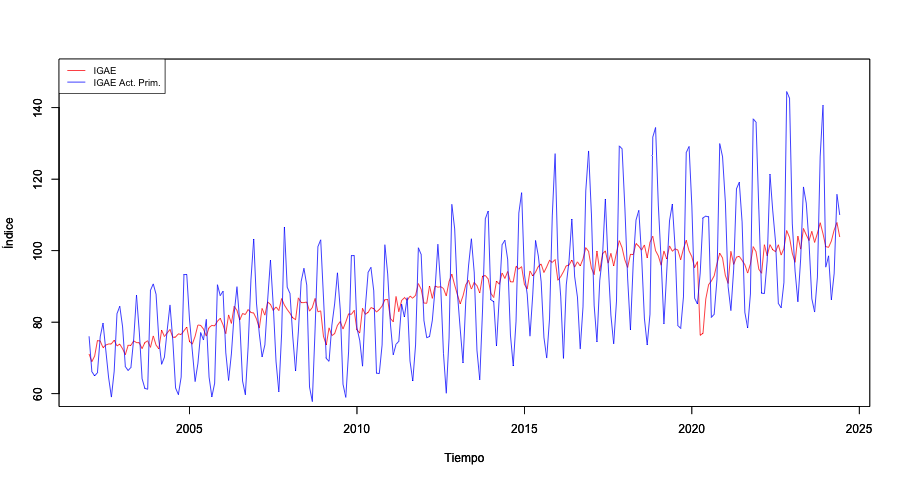
\includegraphics[width=4.16667in,height=3.125in]{Portada.jpg}

\hypertarget{contexto-del-documento}{%
\section*{Contexto del documento}\label{contexto-del-documento}}
\addcontentsline{toc}{section}{Contexto del documento}

Estas son notas de clase de la materia de Análisis de Series de Tiempo de la Facultad de Economía de la Universidad Nacional Autónoma de México y de la Clase de Econometría III del Tecnológico de Monterrey.

Este es un trabajo siempre en proceso de mejora. Para cualquier comentario o aclaración escribir a los correos \href{mailto:benjov@ciencias.unam.mx}{\nolinkurl{benjov@ciencias.unam.mx}} o \href{mailto:omarxalpha@gmail.com}{\nolinkurl{omarxalpha@gmail.com}}.

La versión PDF de estas notas se encuentra en: \url{https://github.com/benjov/Series-Tiempo/blob/main/docs/Notas-Series-Tiempo.pdf}

Las tablas de datos empleadas en los diferentes ejemplos se encuentran en: \url{https://github.com/benjov/Series-Tiempo/tree/main/BD}

\hypertarget{introducciuxf3n}{%
\chapter{Introducción}\label{introducciuxf3n}}

Estas notas son un resumen, una síntesis comparativa y, en algunos casos, una interpretación propia de los libros de texto de Brooks (2019), Cowpertwait y Metcalfe (2009), Guerrero-Guzmán (2014), Enders (2015), Franses y van Dijk (2003), Kirchgassner, Wolters, y Hassler (2012), Lutkepohl (2005), Wei (2019), entre otros. En algunos casos se incorpora información adicional para efectos de dar contexto al tema analizado (ver sección de Bibliografía para mayores detalles).

El objetivo de este documento es proporcionar un conjunto de apuntes o notas que sirvan de apoyo para la clase de Series de Tiempo en la Facultad de Economía de la UNAM. Por esta razón, no deben considerarse como notas exhaustivas o como un sustituto de la clase y los laboratorios. Asimismo, es deseable que los alumnos puedan aportar sus observaciones y correcciones a estas notas, las observaciones a estas notas son esperadas y siempre serán bienvenidas y agradecidas.

Este es un trabajo siempre en proceso de mejora, para cualquier comentario o aclaración, contactar al correo \href{mailto:benjov@ciencias.unam.mx}{\nolinkurl{benjov@ciencias.unam.mx}} o \href{mailto:omarxalpha@gmail.com}{\nolinkurl{omarxalpha@gmail.com}}.

En estas notas se estudian los temas que típicamente son incluidos como parte de un curso estándar de análisis de series de tiempo y agrega otros tantos, los cuales son:

\begin{enumerate}
\def\labelenumi{\arabic{enumi}.}
\item
  Modelos estacionarios univaraidos: \(AR(p)\), \(MA(q)\), \(ARMA(p, q)\) y \(ARIMA(p, d, q)\), y filtros para eliminar estacionalidad, entre otros;
\item
  Modelos no estacionarios univariados y Pruebas de raíz unitaria (o pruebas para determinar que una serie es estacionaria);
\item
  Modelos multivariados, entre lo que se incluye a los Vectores Autoregresivos (VAR) y los procedimientos de Cointegración
\item
  Modelación de series univariadas con errores con heterocedasticidad y autocorrelación: ARCH(r), GARCH(n), etc.;
\item
  Modelos multivariados con errores con heterocedasticidad y autocorrelación: M-GARCH y M-GARCH-M;
\item
  Casos particulares en los que las series incluidas en un modelo multivariado no son del mismo orden de integración, conocidos como modelos ADRL.
\item
  Modelos de Datos Panel en series de tiempo, y
\item
  Modelos no lineales como los de cambios de régimen.
\end{enumerate}

\hypertarget{introducciuxf3n-al-anuxe1lisis-de-series-de-tiempo-y-elementos-de-ecuaciones-en-diferencia}{%
\chapter{Introducción al Análisis de Series de Tiempo y Elementos de Ecuaciones en Diferencia}\label{introducciuxf3n-al-anuxe1lisis-de-series-de-tiempo-y-elementos-de-ecuaciones-en-diferencia}}

\hypertarget{la-naturaleza-de-los-datos-de-series-de-tiempo}{%
\section{La naturaleza de los datos de Series de Tiempo}\label{la-naturaleza-de-los-datos-de-series-de-tiempo}}

El análisis de series de tiempo tiene muchas aplicaciones en diversos campos de la ciencia. Por ejemplo, en la economía continuamente se está expuesto a información recopilada de los mercados financieros, indicadores de empleo, índices o indicadores del nivel de producción, índices de precios, etc. En otros campos de las ciencias sociales se emplea el análisis de series de tiempo para analizar la evolución de la población, los nacimientos, o el número de personas con matrículas escolares. Finalmente, en las ciencias exactas se pueden encontrar casos como los de un epidemiólogo que puede estar interesado en el número de casos de influenza observados en algún periodo de tiempo dado y si a estos se les puede asociar con algún tipo de estacionalidad o si se trata del inicio de un fenómeno atípico.

La primera aproximación que se suele tener a las series de tiempo es mediante el examen de datos puestos en una gráfica, en la cual uno de los ejes es el tiempo y el otro es el valor tomado por la variable. No obstante, en este tipo de exámenes existen dos enfoques. Por un lado, existe el enfoque de la importancia del tiempo, el cual consiste en reconocer cómo lo que sucede hoy es afectado por lo que pasó ayer o, en general, en períodos pasados, o cómo lo que pasa hoy afectará los eventos futuros. Por otro lado, existe el enfoque del análisis frecuentista o de frecuencia, mediante el cual se busca reconocer la importancia que tiene para los investigadores los ciclos --por ejemplo, ciclos estacionales, momentos de crisis económicas, etc.--

\hypertarget{ejemplos-y-aplicaciones-de-las-series-de-tiempo}{%
\section{Ejemplos y aplicaciones de las Series de Tiempo}\label{ejemplos-y-aplicaciones-de-las-series-de-tiempo}}

Un primer ejemplo que puede ilustrar la presencia de los dos tipos de
enfoques antes mencionados es la Figura \ref{fig:fig1}. En esta figura se muestra la evolución del Indicador Global de la Actividad Económica (IGAE) en su versión global o del total de la economía y en su versión únicamente para las actividades primarias entre enero de 2002 y mayo de 2023.

\begin{Shaded}
\begin{Highlighting}[]
\FunctionTok{library}\NormalTok{(readxl)}

\NormalTok{Base\_1 }\OtherTok{\textless{}{-}} \FunctionTok{read\_excel}\NormalTok{(}\StringTok{"BD/Base\_1\_TimeSeries.xlsx"}\NormalTok{)}
\NormalTok{IGAE\_2013 }\OtherTok{\textless{}{-}} \FunctionTok{ts}\NormalTok{(Base\_1}\SpecialCharTok{$}\NormalTok{IGAE\_2013, }\AttributeTok{start =} \DecValTok{2002}\NormalTok{, }\AttributeTok{freq =} \DecValTok{12}\NormalTok{)}
\NormalTok{IGAE\_PRIM\_2013 }\OtherTok{\textless{}{-}} \FunctionTok{ts}\NormalTok{(Base\_1}\SpecialCharTok{$}\NormalTok{IGAE\_PRIM\_2013, }\AttributeTok{start =} \DecValTok{2002}\NormalTok{, }\AttributeTok{freq =} \DecValTok{12}\NormalTok{) }
\NormalTok{ICC }\OtherTok{\textless{}{-}} \FunctionTok{ts}\NormalTok{(Base\_1}\SpecialCharTok{$}\NormalTok{ICC, }\AttributeTok{start =} \DecValTok{2002}\NormalTok{, }\AttributeTok{freq =} \DecValTok{12}\NormalTok{)}
\NormalTok{ICC\_LAG }\OtherTok{\textless{}{-}} \FunctionTok{ts}\NormalTok{(Base\_1}\SpecialCharTok{$}\NormalTok{ICC\_LAG, }\AttributeTok{start =} \DecValTok{2002}\NormalTok{, }\AttributeTok{freq =} \DecValTok{12}\NormalTok{)}
\NormalTok{IPC\_BMV }\OtherTok{\textless{}{-}} \FunctionTok{ts}\NormalTok{(Base\_1}\SpecialCharTok{$}\NormalTok{IPC\_BMV, }\AttributeTok{start =} \DecValTok{2002}\NormalTok{, }\AttributeTok{freq =} \DecValTok{12}\NormalTok{)}
\NormalTok{TDC }\OtherTok{\textless{}{-}} \FunctionTok{ts}\NormalTok{(Base\_1}\SpecialCharTok{$}\NormalTok{TDC, }\AttributeTok{start =} \DecValTok{2002}\NormalTok{, }\AttributeTok{freq =} \DecValTok{12}\NormalTok{)}

\FunctionTok{plot}\NormalTok{(IGAE\_2013, }\AttributeTok{type =} \StringTok{"l"}\NormalTok{, }\AttributeTok{lwd =} \DecValTok{1}\NormalTok{, }\AttributeTok{col =} \StringTok{"red"}\NormalTok{, }\AttributeTok{ylab =} \StringTok{"Indice"}\NormalTok{, }
     \AttributeTok{xlab =} \StringTok{"Tiempo"}\NormalTok{, }\AttributeTok{ylim =} \FunctionTok{c}\NormalTok{(}\DecValTok{60}\NormalTok{,}\DecValTok{160}\NormalTok{)) }
\FunctionTok{par}\NormalTok{(}\AttributeTok{new =}\NormalTok{ T) }
\CommentTok{\# Indicador Global de la Actividad Económica, Act. Prim., base 2008}
\FunctionTok{plot}\NormalTok{(IGAE\_PRIM\_2013, }\AttributeTok{type =} \StringTok{"l"}\NormalTok{, }\AttributeTok{lwd =} \DecValTok{1}\NormalTok{, }\AttributeTok{col =} \StringTok{"blue"}\NormalTok{, }
     \AttributeTok{ylab =} \StringTok{"Indice"}\NormalTok{, }\AttributeTok{xlab =} \StringTok{"Tiempo"}\NormalTok{, }\AttributeTok{ylim =} \FunctionTok{c}\NormalTok{(}\DecValTok{60}\NormalTok{,}\DecValTok{160}\NormalTok{))}
\CommentTok{\# Leyenda}
\FunctionTok{legend}\NormalTok{(}\StringTok{"topleft"}\NormalTok{, }\FunctionTok{c}\NormalTok{(}\StringTok{"IGAE"}\NormalTok{,}\StringTok{"IGAE Act. Prim."}\NormalTok{), }\AttributeTok{cex =} \FloatTok{0.8}\NormalTok{, }
       \AttributeTok{lty =} \DecValTok{1}\SpecialCharTok{:}\DecValTok{1}\NormalTok{, }\AttributeTok{col =} \FunctionTok{c}\NormalTok{(}\StringTok{"red"}\NormalTok{, }\StringTok{"blue"}\NormalTok{))}
\end{Highlighting}
\end{Shaded}

\begin{figure}

{\centering 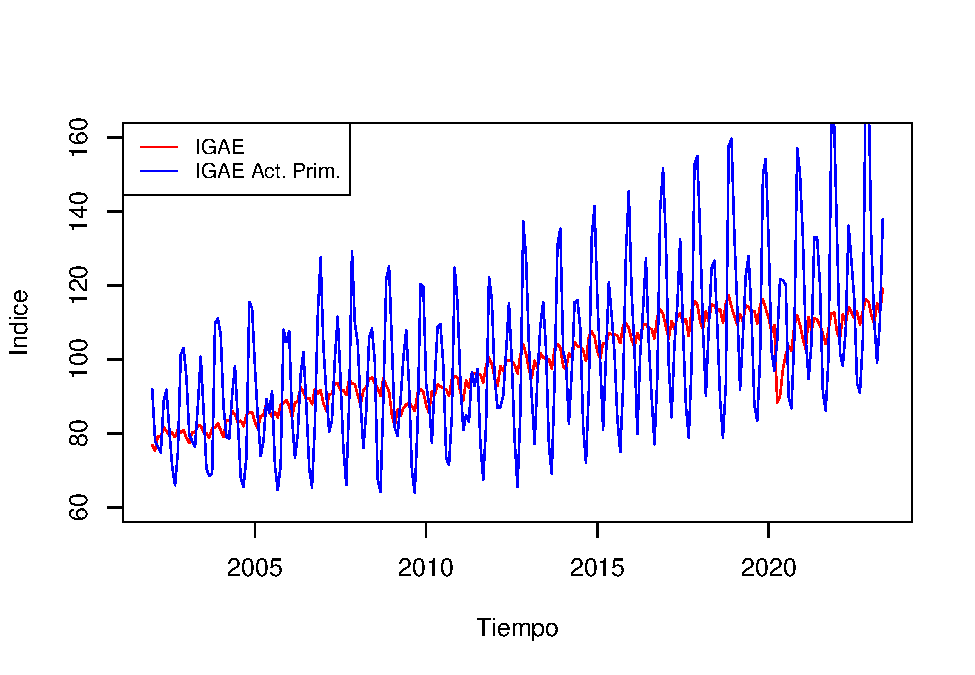
\includegraphics{Notas-Series-Tiempo_files/figure-latex/fig1-1} 

}

\caption{Indicador Global de Actividad Económica (IGAE) Global y para las Actividades Primarias (2008=100), Ene.2002 - May.2023}\label{fig:fig1}
\end{figure}

\begin{Shaded}
\begin{Highlighting}[]
\FunctionTok{par}\NormalTok{(}\AttributeTok{new =}\NormalTok{ F)}
\end{Highlighting}
\end{Shaded}

Como se puede observar, el IGAE del total de la economía muestra, principalmente, que el enfoque del tiempo es más relevante. Es decir, que existe cierta persistencia en el indicador, lo que significa que la economía crece en razón del crecimiento reportado en períodos pasados. No obstante, lo que no podemos reconocer es que los eventos futuros tienen un efecto en el desempeño de la economía hoy día. Así, no es común observar cambios abruptos del indicador, salvo por la crisis global de 2008 y la reciente crisis causada por la COVID-19.

Por el contrario, el IGAE de las actividades primarias muestra una presencia significativa de la importancia de la frecuencia. No pasa desapercibido que existen muchos ciclos en la evolución del indicador. Algo que suena común en las actividades primarias, cuya producción depende de eventos que son cíclicos y que están asociados con el clima u otros factores determinantes de la oferta de productos agrícolas. Otro factor que puede influir en el indicador son elementos de demanda, más que los de oferta. Por ejemplo, el consumo de alimentos típicos de algunas temporadas del año.

Como segundo ejemplo, en la Figura \ref{fig:fig2} se ilustra la evolución reciente del índice de Confianza del Consumidor (ICC) en dos de sus versiones: i) el Índice global y ii) el Índice de confianza de los consumidores cuando estos consideran la situación actual en la economía en relación el año anterior.

\begin{Shaded}
\begin{Highlighting}[]
\FunctionTok{plot}\NormalTok{(ICC, }\AttributeTok{type =} \StringTok{"l"}\NormalTok{, }\AttributeTok{lwd =} \DecValTok{1}\NormalTok{, }\AttributeTok{col =} \StringTok{"red"}\NormalTok{, }\AttributeTok{ylab =} \StringTok{"Indice"}\NormalTok{, }
     \AttributeTok{xlab =} \StringTok{"Tiempo"}\NormalTok{, }\AttributeTok{ylim =} \FunctionTok{c}\NormalTok{(}\DecValTok{29}\NormalTok{, }\DecValTok{50}\NormalTok{))}
\CommentTok{\# Comando que indica a R que sin borrar la grafica anterior, }
\CommentTok{\# grafique la siguiente.}
\FunctionTok{par}\NormalTok{(}\AttributeTok{new =}\NormalTok{ T) }
\CommentTok{\# Indice ??Como considera usted la situacion economica del pais }
\CommentTok{\# hoy en dia comparada con la de hace 12 meses?, base enero 2003}
\FunctionTok{plot}\NormalTok{(ICC\_LAG, }\AttributeTok{type =} \StringTok{"l"}\NormalTok{, }\AttributeTok{lwd =} \DecValTok{1}\NormalTok{, }\AttributeTok{col =} \StringTok{"blue"}\NormalTok{, }\AttributeTok{ylab =} \StringTok{"Indice"}\NormalTok{, }
     \AttributeTok{xlab =} \StringTok{"Tiempo"}\NormalTok{, }\AttributeTok{ylim =} \FunctionTok{c}\NormalTok{(}\DecValTok{29}\NormalTok{,}\DecValTok{50}\NormalTok{))}
\CommentTok{\# Leyenda}
\FunctionTok{legend}\NormalTok{(}\StringTok{"bottomleft"}\NormalTok{, }\FunctionTok{c}\NormalTok{(}\StringTok{"ICC"}\NormalTok{,}\StringTok{"ICC lag"}\NormalTok{), }\AttributeTok{cex =} \FloatTok{0.8}\NormalTok{, }\AttributeTok{lty =} \DecValTok{1}\SpecialCharTok{:}\DecValTok{1}\NormalTok{, }
       \AttributeTok{col =} \FunctionTok{c}\NormalTok{(}\StringTok{"red"}\NormalTok{, }\StringTok{"blue"}\NormalTok{))}
\end{Highlighting}
\end{Shaded}

\begin{figure}

{\centering 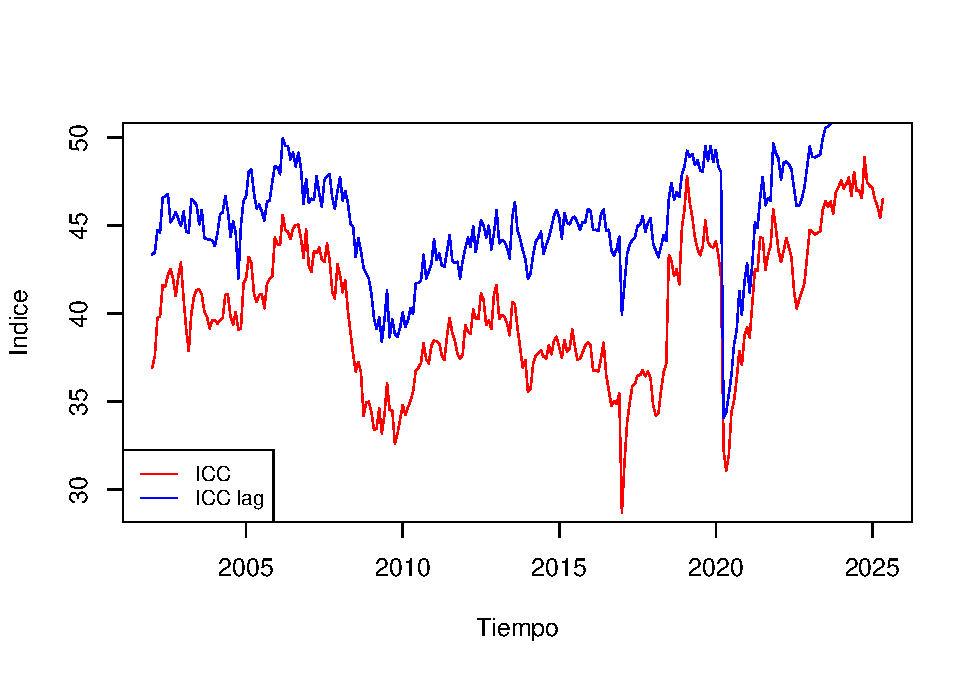
\includegraphics{Notas-Series-Tiempo_files/figure-latex/fig2-1} 

}

\caption{Índice de Confianza del Consumidor (ICC): General y resultado de ¿Cómo considera usted la situación economica del país hoy en día comparada con la de hace 12 meses? (puntos), Ene.2002-may.2023}\label{fig:fig2}
\end{figure}

\begin{Shaded}
\begin{Highlighting}[]
\FunctionTok{par}\NormalTok{(}\AttributeTok{new =}\NormalTok{ F)}
\end{Highlighting}
\end{Shaded}

Destacamos que el ICC mide las expectativas de los consumidores en razón de la información pasada y de la esperada, según dichos consumidores. Así, es probable que las dos series de tiempo exhiban un gran peso para los eventos pasados, pero a la vez, un componente --probablemente menor-- del componente de frecuencia. Esto último en razón de que los consumidores suelen considerar en sus expectativas de consumo los períodos cíclicos de la economía: temporadas navideñas, pagos de colegiaturas, etc. Este segundo ejemplo también ilustra que la confianza del consumidor no necesariamente está directamente correlacionada con el desempeño de la economía.

Como tercer ejemplo se muestra la evolución de dos series. La Figura \ref{fig:fig3} ilustra el comportamiento reciente de dos indicadores que son referencia para los inversionistas. Por un lado, se ubica el índice de Precios y Cotizaciones de la BMV (IPC), el cual refleja el valor de las acciones de empresas que cotizan en la BMV y el volumen de acciones comercializadas, en conjunto. En el mundo de las finanzas se ha interpretado que el IPC refleja el rendimiento del capital promedio invertido en las empresas que cotizan en la BMV.

\begin{Shaded}
\begin{Highlighting}[]
\FunctionTok{par}\NormalTok{(}\AttributeTok{mfrow=}\FunctionTok{c}\NormalTok{(}\DecValTok{1}\NormalTok{,}\DecValTok{2}\NormalTok{))}

\CommentTok{\# Indice de Precios y Cotizaciones de la Bolsa Mexicana de Valores}
\FunctionTok{plot}\NormalTok{(IPC\_BMV, }\AttributeTok{type =} \StringTok{"l"}\NormalTok{, }\AttributeTok{lwd =} \DecValTok{1}\NormalTok{, }\AttributeTok{col =} \StringTok{"red"}\NormalTok{, }\AttributeTok{ylab =} \StringTok{"Indice"}\NormalTok{, }
     \AttributeTok{xlab =} \StringTok{"Tiempo"}\NormalTok{, }\AttributeTok{main =} \StringTok{"Indice de Precios y }\SpecialCharTok{\textbackslash{}n}\StringTok{Cotizaciones BMV"}\NormalTok{)}
\CommentTok{\# Tipo de Cambio para Solventar Obligaciones en Moneda Extranjera}
\FunctionTok{plot}\NormalTok{(TDC, }\AttributeTok{type =} \StringTok{"l"}\NormalTok{, }\AttributeTok{lwd =} \DecValTok{1}\NormalTok{, }\AttributeTok{col =} \StringTok{"blue"}\NormalTok{, }\AttributeTok{ylab =} \StringTok{"Pesos X Dolar"}\NormalTok{, }
     \AttributeTok{xlab =} \StringTok{"Tiempo"}\NormalTok{, }\AttributeTok{main =} \StringTok{"Tipo de Cambio"}\NormalTok{)}
\end{Highlighting}
\end{Shaded}

\begin{figure}

{\centering 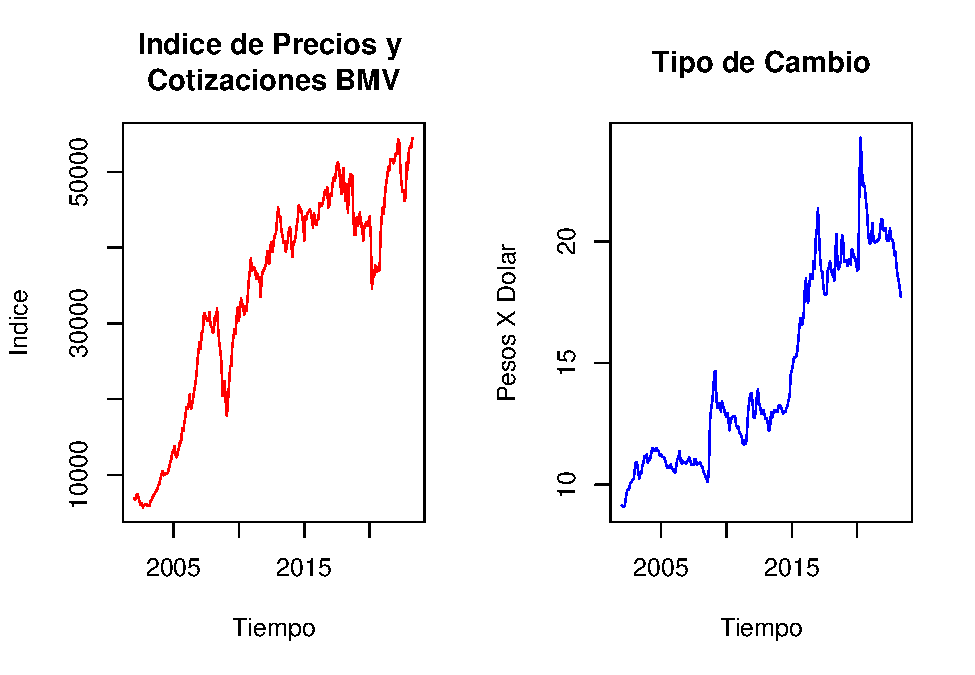
\includegraphics{Notas-Series-Tiempo_files/figure-latex/fig3-1} 

}

\caption{índice de Precios y Cotizaciones de la Bolsa Mexicana de Valores (Panel Derecho) y Tipo de Cambio para Solventar Obligaciones en Moneda Extranjera, pesos por dólar (Panel izquierdo), Ene.2002-May.2023}\label{fig:fig3}
\end{figure}

\begin{Shaded}
\begin{Highlighting}[]
\FunctionTok{par}\NormalTok{(}\AttributeTok{mfrow=}\FunctionTok{c}\NormalTok{(}\DecValTok{1}\NormalTok{,}\DecValTok{1}\NormalTok{))}
\end{Highlighting}
\end{Shaded}

Por otro lado, en la Figura \ref{fig:fig3} se presenta la evolución del Tipo de Cambio (TDC) --indicador financiero que se suele utilizar como medio de reserva de valor--. Esto, en razón de que el TDC es conocido como un instrumento que en momentos de crisis toma valores contracíclicos de la economía mexicana. No obstante, ambos indicadores no son comparables. Para hacerlos comparables en la Figura \ref{fig:fig4} se presentan en versión índice con una base en el primer mes de la muestra.

\begin{Shaded}
\begin{Highlighting}[]
\NormalTok{IPC\_BMV\_I }\OtherTok{\textless{}{-}} \DecValTok{100}\SpecialCharTok{*}\NormalTok{IPC\_BMV}\SpecialCharTok{/}\NormalTok{IPC\_BMV[}\DecValTok{1}\NormalTok{]}
\NormalTok{TDC\_I }\OtherTok{\textless{}{-}} \DecValTok{100}\SpecialCharTok{*}\NormalTok{TDC}\SpecialCharTok{/}\NormalTok{TDC[}\DecValTok{1}\NormalTok{]}
\CommentTok{\# Indice del indice de Precios y Cotizaciones de la Bolsa Mexicana }
\CommentTok{\# de Valores}
\FunctionTok{plot}\NormalTok{(IPC\_BMV\_I, }\AttributeTok{type =} \StringTok{"l"}\NormalTok{, }\AttributeTok{lwd =} \DecValTok{1}\NormalTok{, }\AttributeTok{col =} \StringTok{"red"}\NormalTok{, }\AttributeTok{ylab =} \StringTok{"Indice"}\NormalTok{, }
     \AttributeTok{xlab =} \StringTok{"Tiempo"}\NormalTok{, }\AttributeTok{ylim =} \FunctionTok{c}\NormalTok{(}\DecValTok{80}\NormalTok{,}\DecValTok{740}\NormalTok{))}
\CommentTok{\# Comando que indica a R que sin borrar la grafica anterior, }
\CommentTok{\# grafique la siguiente.}
\FunctionTok{par}\NormalTok{(}\AttributeTok{new =}\NormalTok{ T)}
\CommentTok{\# Indice del Tipo de Cambio para Solventar Obligaciones en }
\CommentTok{\# Moneda Extranjera}
\FunctionTok{plot}\NormalTok{(TDC\_I, }\AttributeTok{type =} \StringTok{"l"}\NormalTok{, }\AttributeTok{lwd =} \DecValTok{1}\NormalTok{, }\AttributeTok{col =} \StringTok{"blue"}\NormalTok{, }\AttributeTok{ylab =} \StringTok{"Indice"}\NormalTok{, }
     \AttributeTok{xlab =} \StringTok{"Tiempo"}\NormalTok{, }\AttributeTok{ylim =} \FunctionTok{c}\NormalTok{(}\DecValTok{80}\NormalTok{,}\DecValTok{740}\NormalTok{))}
\CommentTok{\# Leyenda}
\FunctionTok{legend}\NormalTok{(}\StringTok{"topleft"}\NormalTok{, }\FunctionTok{c}\NormalTok{(}\StringTok{"Indice del IPC"}\NormalTok{,}\StringTok{"Indice del TDC"}\NormalTok{), }\AttributeTok{cex =} \FloatTok{0.8}\NormalTok{, }
       \AttributeTok{lty =} \DecValTok{1}\SpecialCharTok{:}\DecValTok{1}\NormalTok{, }\AttributeTok{col =} \FunctionTok{c}\NormalTok{(}\StringTok{"red"}\NormalTok{, }\StringTok{"blue"}\NormalTok{))}
\end{Highlighting}
\end{Shaded}

\begin{figure}

{\centering 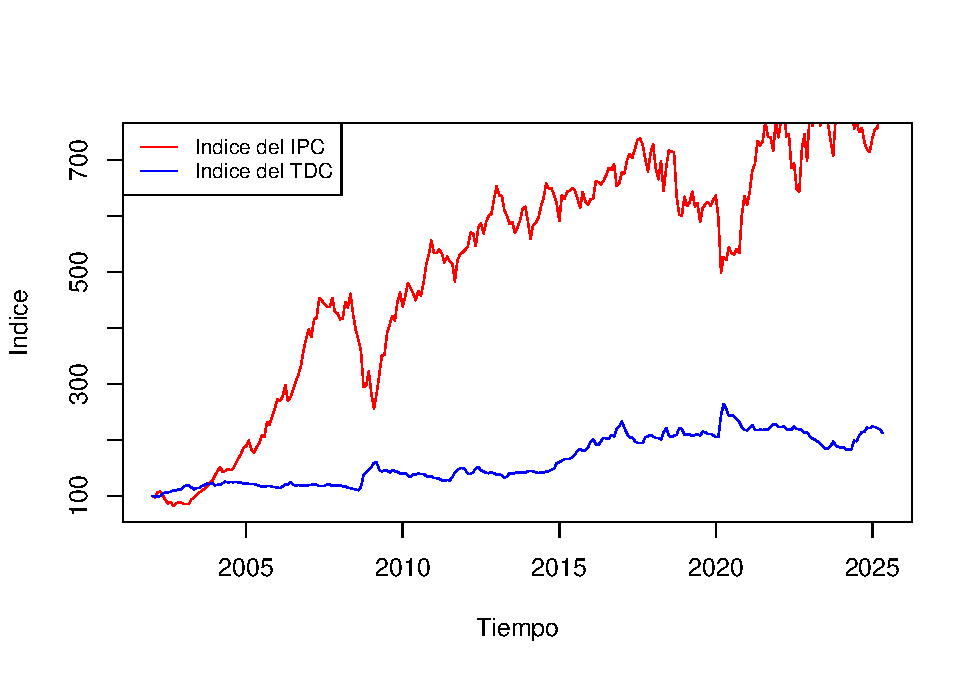
\includegraphics{Notas-Series-Tiempo_files/figure-latex/fig4-1} 

}

\caption{Índice del índice de Precios y Cotizaciones de la Bolsa Mexicana de Valores e Índice del Tipo de Cambio para Solventar Obligaciones en Moneda Extranjera (ambos, enero de 2002 = 100), pesos por dólar, Ene.2002-May.2023 }\label{fig:fig4}
\end{figure}

\begin{Shaded}
\begin{Highlighting}[]
\FunctionTok{par}\NormalTok{(}\AttributeTok{new =}\NormalTok{ F)}
\end{Highlighting}
\end{Shaded}

En la perspectiva de la Figura \ref{fig:fig4} se puede apreciar que el TDC no es tan rentable, ya que una inversión en la BMV mediante el IPC, en el largo plazo, muestra más rendimientos. Asimismo, la Figura \ref{fig:fig4} ilustra que en ambas series se observa un dominio de la condición de tiempo y no uno de la frecuencia. Es decir, tanto el IPC como el TDC no responden a condiciones como ciclos o temporadas que sí son observables en actividades económicas como las
primarias.

Finalmente, la Figura \ref{fig:fig5} ilustra una característica que también resulta de gran interés en el análisis de series de tiempo: los datos de alta frecuencia y de comportamiento no regular. En la Figura \ref{fig:fig5} se muestran las diferencias logarítmicas de las series de IGAE de la actividad total, el IPC y el TDC.

\begin{Shaded}
\begin{Highlighting}[]
\FunctionTok{par}\NormalTok{(}\AttributeTok{mfrow=}\FunctionTok{c}\NormalTok{(}\DecValTok{3}\NormalTok{,}\DecValTok{1}\NormalTok{))}
\CommentTok{\# Indicador Global de la Actividad Econ?mica, base 2008}
\FunctionTok{plot}\NormalTok{(}\FunctionTok{diff}\NormalTok{(}\FunctionTok{log}\NormalTok{(IGAE\_2013), }\AttributeTok{lag =} \DecValTok{1}\NormalTok{), }\AttributeTok{type =} \StringTok{"l"}\NormalTok{, }\AttributeTok{lwd =} \DecValTok{1}\NormalTok{, }
     \AttributeTok{col =} \StringTok{"darkred"}\NormalTok{, }\AttributeTok{ylab =} \StringTok{"Var. \%"}\NormalTok{, }\AttributeTok{xlab =} \StringTok{"Tiempo"}\NormalTok{, }
     \AttributeTok{main =} \StringTok{"Indicador Global de la Actividad Economica"}\NormalTok{) }
\CommentTok{\# Indice de Precios y Cotizaciones de la Bolsa Mexicana de Valores}
\FunctionTok{plot}\NormalTok{(}\FunctionTok{diff}\NormalTok{(}\FunctionTok{log}\NormalTok{(IPC\_BMV), }\AttributeTok{lag =} \DecValTok{1}\NormalTok{), }\AttributeTok{type =} \StringTok{"l"}\NormalTok{, }\AttributeTok{lwd =} \DecValTok{1}\NormalTok{, }
     \AttributeTok{col =} \StringTok{"darkgreen"}\NormalTok{, }\AttributeTok{ylab =} \StringTok{"Var. \%"}\NormalTok{, }\AttributeTok{xlab =} \StringTok{"Tiempo"}\NormalTok{, }
     \AttributeTok{main =} \StringTok{"Indice de Precios y Cotizaciones BMV"}\NormalTok{)}
\CommentTok{\# Tipo de Cambio para Solventar Obligaciones en Moneda Extranjera}
\FunctionTok{plot}\NormalTok{(}\FunctionTok{diff}\NormalTok{(}\FunctionTok{log}\NormalTok{(TDC), }\AttributeTok{lag =} \DecValTok{1}\NormalTok{), }\AttributeTok{type =} \StringTok{"l"}\NormalTok{, }\AttributeTok{lwd =} \DecValTok{1}\NormalTok{, }
     \AttributeTok{col =} \StringTok{"darkblue"}\NormalTok{, }\AttributeTok{ylab =} \StringTok{"Pesos X Dolar"}\NormalTok{, }\AttributeTok{xlab =} \StringTok{"Tiempo"}\NormalTok{, }
     \AttributeTok{main =} \StringTok{"Tipo de Cambio"}\NormalTok{)}
\end{Highlighting}
\end{Shaded}

\begin{figure}

{\centering 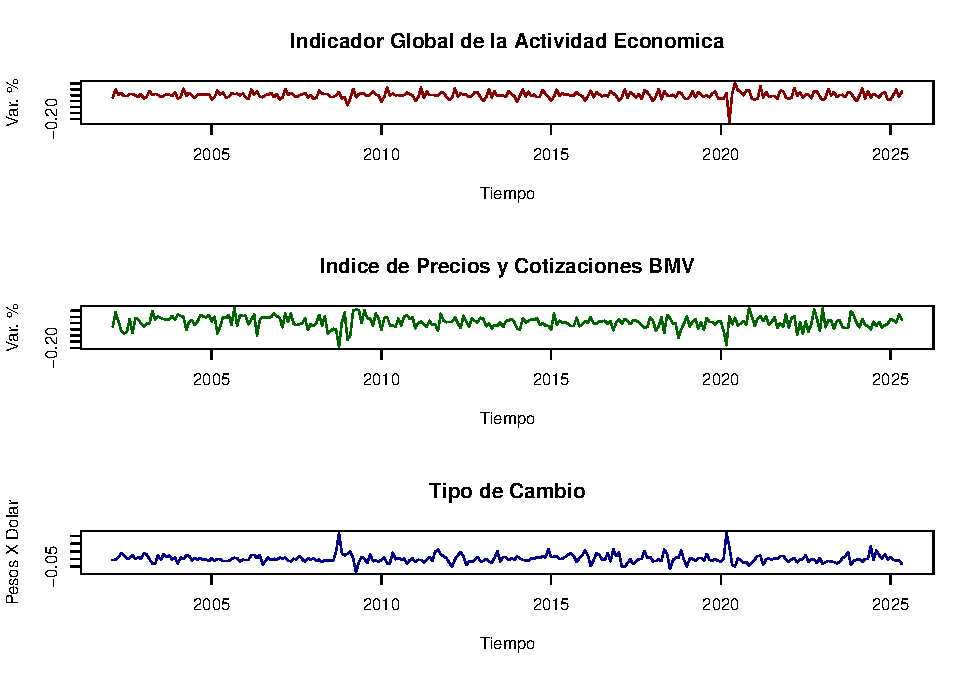
\includegraphics{Notas-Series-Tiempo_files/figure-latex/fig5-1} 

}

\caption{Tasas de Crecimiento mensuales (diferencias logarítmicas) de Indicador Global de la Actividad Económica, Índice de Precios y Cotizaciones de la Bolsa Mexicana de Valores (Panel Derecho) y Tipo de Cambio para Solventar Obligaciones en Moneda Extranjera, Ene.2002-May.2023}\label{fig:fig5}
\end{figure}

\begin{Shaded}
\begin{Highlighting}[]
\FunctionTok{par}\NormalTok{(}\AttributeTok{mfrow=}\FunctionTok{c}\NormalTok{(}\DecValTok{1}\NormalTok{,}\DecValTok{1}\NormalTok{))}
\end{Highlighting}
\end{Shaded}

Dichas diferencias se pueden interpretar como una tasa de crecimiento de las series por las siguientes razones. Consideremos una serie de tiempo dada por \(y_t\), cuya versión logarítmica es \(ln(y_t\)). De esta forma, la diferencia logarítmica está dada por la ecuación \eqref{eq:difflog}:

\begin{equation}
   \Delta ln(y_t) = ln(y_t) - ln(y_{t-1}) = ln \left( \frac{y_t}{y_{t-1}} \right)
   \label{eq:difflog}
\end{equation}

Ahora bien, si retomamos la definición de tasa de crecimiento (\(TC\)) de una serie de tiempo \(y_t\) entre el periodo \(t\) y \(t-1\) podemos obtener que:

\begin{equation}
    TC = \frac{y_t - y_{t-1}}{y_{t-1}} = \frac{y_t}{y_{t-1}} - 1
    \label{eq:TC}
\end{equation}

De esta forma, si tomamos el logaritmo de la expresión de la ecuación \eqref{eq:TC} obtenemos la siguiente aproximación:

\begin{equation}
    \frac{y_t}{y_{t-1}} -1  \approx ln \left( \frac{y_t}{y_{t-1}} \right) = ln(y_t) - ln(y_{t-1})
    \label{eq:TCDiffLog}
\end{equation}

La ecuación \eqref{eq:TCDiffLog} es cierta cuando los valores de \(y_t\) y \(y_{t-1}\) son muy parecidos, es decir, cuando las variaciones no son tan abruptas. Otra forma de interpretar la ecuación \eqref{eq:TCDiffLog} es que para tasas de crecimiento pequeñas, se puede utilizar como una buena aproximación a la diferencia logarítmica mostrada en la ecuación \eqref{eq:difflog}.

En la Figura \ref{fig:fig5} se reportan las diferencias logarítmicas del IGAE, IPC y TDC, todos, como una media de distintos tipos de rendimientos. Es decir, podemos decir que un capitalista promedio (suponiendo que solo puede invertir en la actividad económica, en la bolsa o en el dólar), puede observar que le es más redituable en función de sus preferencias.

Notése que la dinámica de las variaciones de cada una de las series es significativamente diferente. Destaca que el TDC es una de las variables que, en general, no muestra grandes cambios a lo largo del tiempo. No obstante, se han observado cambios radicales, cuando menos en el año 2008 y durante la pandemia de COVID-19. Esta situación también se ha observado para el IPC. En cambio, el IGAE muestra un comportamiento más estable o estacionario --concepto que abordaremos más adelante--.

\hypertarget{ecuaciones-en-diferencia-para-procesos-deterministas}{%
\section{Ecuaciones en Diferencia para procesos deterministas}\label{ecuaciones-en-diferencia-para-procesos-deterministas}}

En las secciones previas se hizo una introducción al concepto de series de tiempo. En esta sección se pretende desarrollar la construcción de los procesos generadores de datos de las series de tiempo. En un sentido más formal, se expondrá que las series de tiempo se pueden considerar como una secuencia de variables aleatorias.

Para tales efectos, se desarrollará una introducción al concepto de ecuaciones en diferencia. Así, las preguntas que se pretende responder son:

\begin{enumerate}
\def\labelenumi{\arabic{enumi}.}
\item
  ¿Cuál es la solución de la ecuación en diferencia que se estudia?
\item
  ¿Cuáles son las condiciones para que un proceso estocástico, representado mediante una ecuación en diferencia, llegue a alcanzar un punto de equilibrio en el largo plazo?
\end{enumerate}

El término de \emph{ecuación en diferencia} sirve para denominar un proceso similar o equivalente dentro de las ecuaciones diferenciales, dentro del cual se consideran a un conjunto de variables que están en función del tiempo. Así, si consideramos al tiempo como una variable continua, es decir, consideramos una variable \(Z(t)\), podemos expresar las siguientes expresiones para la ecuación diferencial:
\begin{equation}
    \frac{dZ(t)}{dt}; \frac{d^2Z(t)}{dt^2}; \ldots; \frac{d^kZ(t)}{dt^k}
        \label{eq:eqDiff}
\end{equation}

Por otro lado, suponiendo el caso del tiempo en forma discreta, es decir, con \(t = \ldots, -2, -1, 0, 1, 2, \ldots\), entonces el comportamiento de la serie de variables dadas por \(Z_t\), la cual se puede expresar como:
\begin{equation}
    \Delta Z_t; \Delta^2 Z_t; \ldots; \Delta^k Z_t
    \label{eq:Diff1}
\end{equation}

Observemos que una forma técnicamente más correcta es escribir las expresiones anteriores como:
\begin{equation}
    \frac{\Delta Z_t}{\Delta t}; \frac{\Delta^2 Z_t}{\Delta t^2}; \ldots; \frac{\Delta^k Z_t}{\Delta t^k}
    \label{eq:Diff2}
\end{equation}

No obstante, no pasa desapercibido que \(\Delta t = 1\), por lo que resultan equivalentes ambos conjuntos de expresiones \eqref{eq:Diff1} y \eqref{eq:Diff2}.

\hypertarget{ecuaciones-en-diferencia-lineales-de-primer-orden}{%
\subsection{Ecuaciones en Diferencia Lineales de Primer Orden}\label{ecuaciones-en-diferencia-lineales-de-primer-orden}}

El primer caso que se suele estudiar en relación a Ecuaciones en Diferencia es el de las Ecuaciones en Diferencia Lineales de Primer Orden. Al respecto, al igual que en el caso continuo, las variaciones de la variable \(Z_t\) se pueden expresar como se ilustra en el siguiente ejemplo. Consideremos la siguiente ecuación:
\begin{equation}
    Z_t = a_0 + a_1 Z_{t-1}
    \label{eq:EDPO}
\end{equation}

Donde, \(t = \ldots, -2, -1, 0, 1, 2, \ldots\), y \(a_0\) y \(a_1 \neq 0\) son números reales constantes. De \eqref{eq:EDPO} podemos despejar la variable \(Z_{t-1}\) y obtener una forma de ecuación en diferencia:
\begin{equation}
    Z_t - a_1 Z_{t-1} = a_0
    \label{eq:EDPO2}
\end{equation}

Ahora denotemos a \(L Z_t = Z_{t-1}\), es decir, mediante el operador \(L\) se puede rezagar una variable dada. En general, podemos decir que el operador tiene dos propiedades, la primera es que es lineal --en el sentido de que abre sumas y saca escalares-- como se muestra en la siguiente expresión para el caso de un (1) rezago:
\begin{equation}
    L(\alpha Z_{t} + \beta) = \alpha Z_{t-1} + \beta
    \label{eq:E1Lag}
\end{equation}

Donde \(\alpha, \beta \in \mathbb{R}\) y \(\alpha, \beta \neq 0\). Otro resultado implícito en esta primera propiedad es que el operador rezago aplicado a cualquier escalar dará como resultado el escalar, puesto que este es una constante sin importar el momento \(t\) en el cual se encuentre la variable \(Z\).

La segunda propiedad del operador es que se puede aplicar de forma consecutiva a una misma variable. Es decir, \(L ( Z_{t-1}) = L L Z_{t} = L^2 Z_{t}\), por lo que en general tendremos: \(L^p Z_t = Z_{t-p}\) (con \(p \in \mathbb{Z}\)). Así, en el caso de \(p\) rezagos la propiedad de linealidad del operador rezago será:
\begin{equation}
    L^p (\alpha Z_{t} + \beta) = \alpha Z_{t-p} + \beta
   \label{eq:LinProp}
\end{equation}

Dicho lo anterior, podemos escribir la solución general de \eqref{eq:EDPO2} como:
\begin{eqnarray}
    Z_t - a_1 L Z_t & = & a_0 \nonumber \\
    (1 - a_1 L)Z_t & = & a_0 \nonumber \\
    Z_t & = & a_0 \frac{1}{1 - a_1 L} + s a^t_1 \nonumber \\
    Z_t & = & a_0 \frac{1}{1 - a_1} + s a^t_1
    \label{eq:PROC01}
\end{eqnarray}

Donde \(a_1 \neq 1\) y \(t = \ldots, -2, -1, 0, 1, 2, \ldots\). Notése que la aplicación del operador rezago \(L\) a la constante \(a_1\) dará como resultado el valor de la misma constante, ya que ésta no depende del momento \(t\) en el cual observemos a la variable \(Z_t\). En la ecuación \eqref{eq:PROC01} se adiciona un término \(s a^t_1\) que permite ubicar la trayectoria inicial de la solución de la ecuación. El componente no significa un cambio respecto de la ecuación \eqref{eq:EDPO2} original, ya que si buscáramos reconstruir esta ecuación tendríamos:
\begin{eqnarray}
    (1 - a_1 L) s a^t_1 & = & s a^t_1 - a_1 s L a^{t}_1 \nonumber \\
    & = & s a^t_1 - a_1 s a^{t - 1}_1 \nonumber \\
    & = & s a^t_1 - s a^t_1 \nonumber \\
    & = & 0 \nonumber
\end{eqnarray}

La ecuación \eqref{eq:PROC01} se suele interpretar como la solución de largo plazo. Ahora demostraremos por qué es cierta la ecuación y discutiremos algunas condiciones que se deben observar en esta solución para que sea una solución convergente. No obstante, primero discutiremos un método indirecto e incompleto para demostrar el resultado. Dicho método es conocido como el método iterativo. Plantearemos las siguientes ecuaciones particulares donde suponemos la existencia del valor inicial \(Z_0\) del proceso:
\begin{equation*}
    Z_1 = a_0 + a_1 Z_0
\end{equation*}

\begin{eqnarray*}
Z_2 & = & a_0 + a_1 Z_1 \\
    & = & a_0 + a_1 (a_0 + a_1 Z_0) \\
    & = & a_0 +  a_0 a_1 + a^2_1 Z_0 \\
    & = & a_0 (1 + a_1) + a^2_1 Z_0
\end{eqnarray*}

\begin{eqnarray*}
Z_3 & = & a_0 + a_1 Z_2 \\
    & = & a_0 + a_1 (a_0 +  a_0 a_1 + a^2_1 Z_0) \\
    & = & a_0 +  a_0 a_1 + a_0 a^2_1 + a^3_1 Z_0 \\
    & = & a_0 (1 + a_1 + a^2_1) + a^3_1 Z_0
\end{eqnarray*}

De lo anterior se puede inferir que el método iterativo convergerá hacia una expresión como la siguiente en el momento \(t\):
\begin{eqnarray}
Z_t & = & a_0 + a_1 Z_{t-1} \nonumber \\
    & = & a_0 (1 + a_1 + a^2_1 + \ldots + a^{t-1}_1) + a^t_1 Z_0 \nonumber \\
    & = & a_0 \sum^{t-1}_{i = 0}{a^i_1} + a^t_1 Z_0
    \label{eq:SUM}
\end{eqnarray}

Donde, es necesario que en la ecuación \eqref{eq:SUM} se cumpla que \(\lvert{a_1}\lvert < 1\) para que la suma sea convergente --más adelante detallaremos esta afirmación--. A este tipo de ecuaciones se les puede denominar como lineales. Esto en razón de que ningún término de la variable \(Z\) aparece elevado a ninguna potencia distinta a 1. También, son de primer orden, ya que el rezago de la variable \(Z\) es sólo de un período.

En adelante trabajaremos con ecuaciones en las que la variable \(Z\) se encuentra rezagada en cualquiera de los siguientes casos:
\begin{equation}
    Z_t, Z_{t-1}, Z_{t-2}, Z_{t-3}, \ldots, Z_{t-p}, \ldots
    \label{eq:SUM0}
\end{equation}

Por lo que diremos que en adelante el curso versará sobre ecuaciones en diferencia lineales y de cualquier orden \(p \in \mathbb{N}\).

Retomando la ecuación \eqref{eq:SUM} y considerando la parte de la suma de los términos de \(a^i_1\), de tal forma que buscaremos dar una expresión más comprensible a dicho término. Definamos la siguiente expresión como:
\begin{equation}
    S_{t-1} = \sum^{t-1}_{i = 0}{a^i_1}
    \label{eq:St1}
\end{equation}

Por lo tanto, \(S_t\) estaría dado por la siguiente expresión:
\begin{eqnarray}
S_{t} & = & a_1 \sum^{t-1}_{i = 0}{a^i_1} \nonumber \\
      & = & a_1 (1 + a_1 + a^2_1 + \ldots + a^{t-1}_1) \nonumber \\
      & = & a_1 + a^2_1 + a^3_1 + \ldots + a^{t}_1 \nonumber \\
      & = & a_1 S_{t-1}
      \label{eq:St}
\end{eqnarray}

Tomando los dos resultados de las ecuaciones \eqref{eq:St1} y \eqref{eq:St} anteriores, podemos expresar que si a \(S_{t-1}\) le restamos \(S_t\), y desarrollando ambos lados de la ecuación anterior podemos obtener:
\begin{eqnarray}
    S_{t-1} - a_1 S_{t-1} & = & S_{t-1} - S_{t} \nonumber \\
    (1 - a_1) S_{t-1} & = & (1 + a_1 + a^2_1 + \ldots + a^{t-1}_1) - (a_1 + a^2_1 + a^3_1 + \ldots + a^{t}_1) \nonumber \\
    (1 - a_1) S_{t-1} & = & 1 - a^{t}_1 \nonumber
\end{eqnarray}

Así, podemos concluir que:
\begin{equation}
    S_{t-1} = \frac{1 - a^{t}_1}{1 - a_1}
    \label{eq:SUM2}
\end{equation}

Conjuntando este último resultado de la ecuación \eqref{eq:SUM2} con la ecuación \eqref{eq:SUM} tenemos la siguiente solución por el método de iteración:
\begin{equation}
    Z_t = a_0 \left( \frac{1 - a^{t}_1}{1 - a_1} \right) + a^t_1 Z_0
    \label{eq:SOLITER}
\end{equation}

De esta forma la ecuación \eqref{eq:SOLITER} es una solución para la ecuación \eqref{eq:SUM}, que es una ecuación de un proceso de una Ecuación en Diferencia planteado en la ecuación \eqref{eq:EDPO}. Esta solución aún no es general, en el sentido de que sea válida para cualquier tipo de proceso: convergente o divergente. Dicha convergencia o divergencia estará determinada por el parámetro \(a_1\). No debe pasar desapercibido que cuando \(t \rightarrow \infty\) o cuando la muestra es muy grande (lo que es equivalente), podemos decir que la solución solo puede converger a la siguiente expresión cuando se considera que \(|a_1| < 1\):
\begin{equation}
    Z_t = a_0 \left( \frac{1}{1 - a_1} \right)
    \label{eq:trayec}
\end{equation}

Retomemos ahora el caso general descrito en la ecuación \eqref{eq:PROC01} y determinemos una solución general en la cual \(a_1 \neq 1\) y \(t = \ldots, -2, -1, 0, 1, 2, \ldots\). Para ello, observemos que el siguiente componente en la ecuación mencionada se puede interpretar como la suma infinita de términos descritos como:
\begin{eqnarray}
    \frac{1}{1 - a_1} & = & 1 + a_1 + a_1^2 + \ldots + a_1^t + \ldots \nonumber \\
    & = & \sum_{i = 0}^{\infty} a_1^{i}
    \label{eq:SUMINF}
\end{eqnarray}

Donde claramente es necesario que \(|a_1| < 1\). Por lo tanto, sólo faltaría determinar el valor de la constante \(s\) en la ecuación \eqref{eq:PROC01} de la siguiente forma, supongamos que observamos el proceso en el momento inicial, por lo que es posible determinar el valor de la constante conociendo el valor inicial del proceso como sigue:
\begin{equation}
    Z_0 = a_0 \frac{1}{1 - a_1} + s
\label{eq:Z0}
\end{equation}

De la ecuación \eqref{eq:Z0} tenemos que:
\begin{equation}
    s = Z_0 - a_0 \frac{1}{1 - a_1}
\label{eq:eqs}
\end{equation}

Así, juntando la ecuación \eqref{eq:PROC01} y la ecuación \eqref{eq:eqs} tenemos la expresión:
\begin{equation}
    Z_t = a_0 \frac{1 - a^t_1}{1 - a_1} + a^t_1 Z_0
\label{eq:SOLGEN}
\end{equation}

No debe pasar desapercibido que esta solución es la misma que la mostrada en la ecuación \eqref{eq:SOLITER}, por lo que en realidad ambas ecuaciones son una solución general indistintamente entre las ecuaciones \eqref{eq:SOLITER} y \eqref{eq:SOLGEN}. Ambas convergen a la expresión como la ecuación \eqref{eq:trayec}, con la misma condición de convergencia \(|a_1| < 1\). Para ilustrar estas ecuaciones, veamos algunos ejemplos al respecto.

\textbf{Ejemplo}. Consideremos que tenemos un proceso \(Z_t\) que es descrito por una ecuación en diferencia lineal de primer orden dada por:
\begin{equation}
    Z_t = 2 + 0.9 Z_{t-1}
\label{eq:ex1}
\end{equation}

Siguiendo la expresión mostrada en la ecuación \eqref{eq:SOLGEN}, obtenemos la expresión:
\begin{equation}
    Z_t = 2 \left( \frac{1 - 0.9^{t}}{1 - 0.9} \right) + 0.9^t Z_0
\label{eq:ex2}
\end{equation}

Donde asumiremos que el valor inicial es \(Z_0 = 10\) y que la expresión debe converger al valor de 20, cuando \(t\) es muy grande o tiende a infinito.

\textbf{Ejemplo}. De forma similar, tomemos otro ejemplo en el cual asumimos la siguiente expresión:
\begin{equation}
    Z_t = 2 - 0.5 Z_{t-1}
\label{eq:ex3}
\end{equation}

Siguiendo la expresión mostrada en la ecuación \eqref{eq:SOLGEN}, obtenemos:
\begin{equation}
    Z_t = 2 \left( \frac{1 - (-0.5)^{t}}{1 + 0.5} \right) + (-0.5)^t Z_0
\label{eq:ex4}
\end{equation}

Donde asumiremos que el valor inicial es \(Z_0 = 10\) y que la ecuación converge al valor de \(1.3333333 \ldots\), cuando \(t\) es muy grande o tiende a infinito. Ahora simulemos el comportamiento de ambos procesos y estableceremos los resultados del Cuadro \ref{tab:table1}. Notemos que el segundo proceso converge de una forma más rápida que el primero. El Cuadro \ref{tab:table1} se ilustra en las siguientes dos Figura \ref{fig:fig21} y Figura \ref{fig:fig22}.

\begin{Shaded}
\begin{Highlighting}[]
\FunctionTok{library}\NormalTok{(knitr)}
\FunctionTok{library}\NormalTok{(tidyverse)}
\FunctionTok{library}\NormalTok{(kableExtra)}

\NormalTok{Tiempo }\OtherTok{=} \FunctionTok{c}\NormalTok{(}\DecValTok{0}\SpecialCharTok{:}\DecValTok{100}\NormalTok{)}
\NormalTok{Zt }\OtherTok{=} \FunctionTok{rep}\NormalTok{(}\ConstantTok{NA}\NormalTok{, }\DecValTok{101}\NormalTok{)}
\NormalTok{Zt2 }\OtherTok{=} \FunctionTok{rep}\NormalTok{(}\ConstantTok{NA}\NormalTok{,}\DecValTok{101}\NormalTok{)}
\NormalTok{Zt[}\DecValTok{1}\NormalTok{] }\OtherTok{=} \DecValTok{10}
\NormalTok{Zt2[}\DecValTok{1}\NormalTok{] }\OtherTok{=} \DecValTok{10}

\ControlFlowTok{for}\NormalTok{ (i }\ControlFlowTok{in} \FunctionTok{c}\NormalTok{(}\DecValTok{2}\SpecialCharTok{:}\DecValTok{101}\NormalTok{))\{}
\NormalTok{  Zt[i] }\OtherTok{=} \DecValTok{2}\FloatTok{+0.9}\SpecialCharTok{*}\NormalTok{Zt[i}\DecValTok{{-}1}\NormalTok{]}
\NormalTok{  Zt2[i] }\OtherTok{=} \DecValTok{2} \SpecialCharTok{{-}} \FloatTok{0.5}\SpecialCharTok{*}\NormalTok{Zt2[i}\DecValTok{{-}1}\NormalTok{]}
\NormalTok{\}}
\NormalTok{lista }\OtherTok{=} \FunctionTok{c}\NormalTok{(}\DecValTok{1}\SpecialCharTok{:}\DecValTok{16}\NormalTok{, }\DecValTok{97}\SpecialCharTok{:}\DecValTok{101}\NormalTok{)}
\NormalTok{Tiempo1 }\OtherTok{=}\NormalTok{ Tiempo[lista]}
\NormalTok{Zt1}\OtherTok{=}\NormalTok{Zt[lista]}
\NormalTok{Zt21}\OtherTok{=}\NormalTok{Zt2[lista]}

\NormalTok{tabla1 }\OtherTok{=} \FunctionTok{data.frame}\NormalTok{(Tiempo1, Zt1, Zt21)}
\FunctionTok{colnames}\NormalTok{(tabla1) }\OtherTok{\textless{}{-}} \FunctionTok{c}\NormalTok{(}\StringTok{"Tiempo"}\NormalTok{, }\StringTok{"$Z\_t =2+0.9Z\_\{t{-}1\}$"}\NormalTok{, }
                      \StringTok{"$Z\_t = 2{-}0.5Z\_\{t{-}1\}$"}\NormalTok{)}

\FunctionTok{kable}\NormalTok{(tabla1, }
      \AttributeTok{caption =} \StringTok{"Dos ejemplos de Ecuaciones Lineales de Primer Orden"}\NormalTok{, }
      \AttributeTok{format =} \StringTok{"pandoc"}\NormalTok{) }\SpecialCharTok{\%\textgreater{}\%}
  \FunctionTok{kable\_styling}\NormalTok{(}\AttributeTok{font\_size =} \DecValTok{10}\NormalTok{)}
\end{Highlighting}
\end{Shaded}

\begin{longtable}[]{@{}rrr@{}}
\caption{\label{tab:table1}Dos ejemplos de Ecuaciones Lineales de Primer Orden}\tabularnewline
\toprule\noalign{}
Tiempo & \(Z_t =2+0.9Z_{t-1}\) & \(Z_t = 2-0.5Z_{t-1}\) \\
\midrule\noalign{}
\endfirsthead
\toprule\noalign{}
Tiempo & \(Z_t =2+0.9Z_{t-1}\) & \(Z_t = 2-0.5Z_{t-1}\) \\
\midrule\noalign{}
\endhead
\bottomrule\noalign{}
\endlastfoot
0 & 10.00000 & 10.000000 \\
1 & 11.00000 & -3.000000 \\
2 & 11.90000 & 3.500000 \\
3 & 12.71000 & 0.250000 \\
4 & 13.43900 & 1.875000 \\
5 & 14.09510 & 1.062500 \\
6 & 14.68559 & 1.468750 \\
7 & 15.21703 & 1.265625 \\
8 & 15.69533 & 1.367188 \\
9 & 16.12580 & 1.316406 \\
10 & 16.51322 & 1.341797 \\
11 & 16.86189 & 1.329102 \\
12 & 17.17570 & 1.335449 \\
13 & 17.45813 & 1.332275 \\
14 & 17.71232 & 1.333862 \\
15 & 17.94109 & 1.333069 \\
96 & 19.99960 & 1.333333 \\
97 & 19.99964 & 1.333333 \\
98 & 19.99967 & 1.333333 \\
99 & 19.99970 & 1.333333 \\
100 & 19.99973 & 1.333333 \\
\end{longtable}

\begin{Shaded}
\begin{Highlighting}[]
\NormalTok{tabla }\OtherTok{\textless{}{-}} \FunctionTok{data.frame}\NormalTok{( Tiempo, Zt, Zt2 )}

\FunctionTok{ggplot}\NormalTok{( }\AttributeTok{data =}\NormalTok{ tabla , }\FunctionTok{aes}\NormalTok{(}\AttributeTok{x =}\NormalTok{ Tiempo, }\AttributeTok{y =}\NormalTok{ Zt) )}\SpecialCharTok{+}
  \FunctionTok{geom\_line}\NormalTok{(}\AttributeTok{col=}\StringTok{"blue4"}\NormalTok{) }\SpecialCharTok{+}
  \FunctionTok{geom\_point}\NormalTok{(}\AttributeTok{col=} \StringTok{"blue4"}\NormalTok{) }\SpecialCharTok{+}
  \FunctionTok{labs}\NormalTok{(}\AttributeTok{y=}\FunctionTok{expression}\NormalTok{(Z[t]))}
\end{Highlighting}
\end{Shaded}

\begin{figure}

{\centering 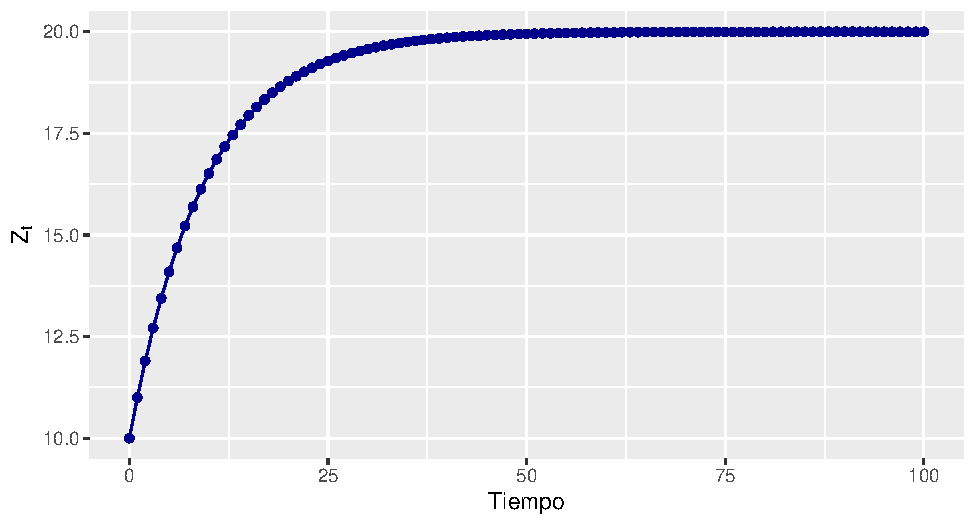
\includegraphics{Notas-Series-Tiempo_files/figure-latex/fig21-1} 

}

\caption{Evolución del proceso dado por $Z_t =2+0.9Z_{t-1}$}\label{fig:fig21}
\end{figure}

\begin{Shaded}
\begin{Highlighting}[]
\FunctionTok{ggplot}\NormalTok{(}\AttributeTok{data =}\NormalTok{ tabla , }\FunctionTok{aes}\NormalTok{(}\AttributeTok{x =}\NormalTok{ Tiempo, }\AttributeTok{y=}\NormalTok{Zt2)) }\SpecialCharTok{+}
  \FunctionTok{geom\_line}\NormalTok{(}\AttributeTok{col=}\StringTok{"red4"}\NormalTok{) }\SpecialCharTok{+}
  \FunctionTok{geom\_point}\NormalTok{(}\AttributeTok{col=} \StringTok{"red4"}\NormalTok{) }\SpecialCharTok{+}
  \FunctionTok{labs}\NormalTok{(}\AttributeTok{y=}\FunctionTok{expression}\NormalTok{(Z[t]))}
\end{Highlighting}
\end{Shaded}

\begin{figure}

{\centering 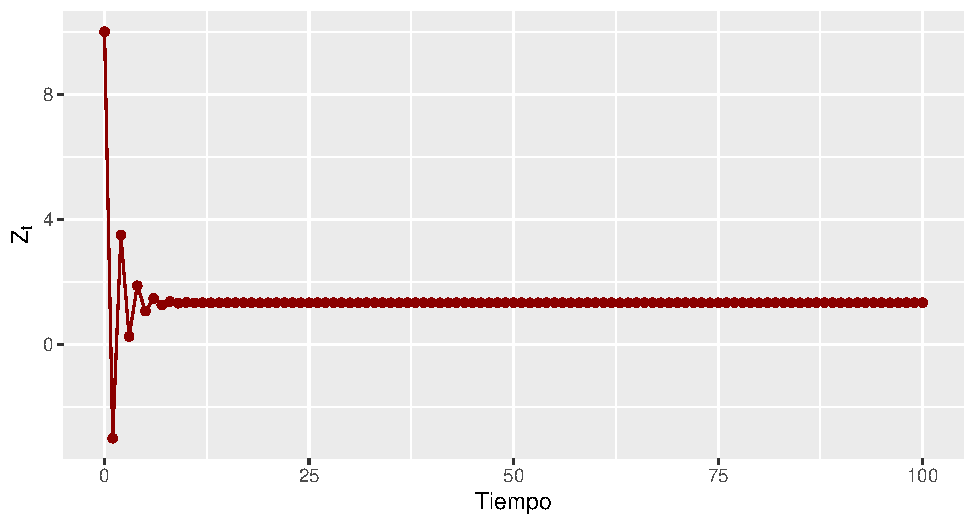
\includegraphics{Notas-Series-Tiempo_files/figure-latex/fig22-1} 

}

\caption{Evolución del proceso dado por $Z_t =2-0.5Z_{t-1}$}\label{fig:fig22}
\end{figure}

\hypertarget{ecuaciones-en-diferencia-lineales-de-segundo-orden-y-de-orden-superior}{%
\subsection{Ecuaciones en Diferencia Lineales de Segundo Orden y de orden superior}\label{ecuaciones-en-diferencia-lineales-de-segundo-orden-y-de-orden-superior}}

Como un segundo caso a estudiar se ubica el caso de las Ecuaciones en Diferencia Lineales de Segundo Orden y, en su caso, de orden superior. Primero, sea una ecuación como la siguiente, la cual es lineal y de segundo orden, ya que tiene asociado un término de \(Z_t\) rezagado dos períodos:
\begin{equation}
    Z_t = a_0 + a_1 Z_{t-1} + a_2 Z_{t-2}
    \label{eq:EDSO}
\end{equation}

Donde \(t = \ldots, -2, -1, 0, 1, 2, \ldots\) y \(a_1, a_2 \neq 0\). Reordenando la ecuación \eqref{eq:EDSO} podemos escribir:
\begin{eqnarray}
    Z_t - a_1 Z_{t-1} - a_2 Z_{t-2} & = & a_0 \nonumber \\
    Z_t - a_1 L Z_{t} - a_2 L^2 Z_{t} & = & a_0 \nonumber \\
    (1 - a_1 L - a_2 L^2)Z_t & = & a_0 
    \label{eq:EDSOSOL}
\end{eqnarray}

Así, la solución general propuesta para la ecuación \eqref{eq:EDSOSOL} es la siguiente, la cual es una forma análoga a una Ecuación Lineal en Diferencia de Primer Orden:
\begin{equation}
    Z_t = \frac{a_0}{1 - a_1 - a_2} + s_1 g^t_1 + s_2 g^t_2
    \label{eq:SOLGEN2}
\end{equation}

En donde \(s_1\) y \(s_2\) son constantes que se determinan mediante dos condiciones iniciales --por lo que para resolver este tipo de ecuaciones requerimos conocer dos condiciones iniciales--. Los valores de \(g_1\) y \(g_2\) están relacionados con los coeficientes \(a_1\) y \(a_2\), de esta forma:
\begin{equation}
  a_1  =  g_1 + g_2
  \label{eq:a1}
\end{equation}

\begin{equation}
    a_2  =  - g_1 g_2
    \label{eq:a2}
\end{equation}

Lo anterior surge del siguiente procedimiento y recordando que siempre es posible descomponer una ecuación cuadrática en expresiones como las siguientes:
\begin{eqnarray}
    (1 - a_1 L - a_2 L^2) & = & (1 - g_1 L)(1 - g_2 L) \nonumber \\
    & = & 1 - g_1 L - g_2 L + g_1 g_2 L^2 \nonumber \\
    & = & 1 - (g_1 + g_2) L + g_1 g_2 L^2
    \label{eq:eqcaracteristica}
\end{eqnarray}

Donde se observa la equivalencia mostrada en las ecuaciones \eqref{eq:a1} y \eqref{eq:a2}. Así, considerando la ecuación \eqref{eq:SOLGEN2} tenemos que:
\begin{eqnarray}
    (1 - a_1 L - a_2 L^2) Z_t & = & (1 - g_1 L)(1 - g_2 L) Z_t \nonumber \\
    & = & a_0 + (1 - g_1 L)(1 - g_2 L) s_1 g^t_1 \nonumber \\
    &  & + (1 - g_1 L)(1 - g_2 L) s_2 g^t_2
    \label{eq:eqcaracteristica1}
\end{eqnarray}

Por lo tanto, buscamos que, para que el proceso sea equivalente y podamos interpretar que la ecuación \eqref{eq:SOLGEN2} sea una solución general, deberá pasar lo siguiente:
\begin{equation}
    (1 - g_1 L) (1 - g_2 L) s_1 g^t_1 + (1 - g_1 L) (1 - g_2 L) s_2 g^t_2 = 0
    \label{eq:eqcaracteristica2}
\end{equation}

O, escrito de otra forma:
\begin{equation}
    (1 - g_1 L) s_1 g^t_1 = (1 - g_2 L) s_2 g^t_2 = 0
    \label{eq:eqcaracteristica3}
\end{equation}

Ahora determinemos cuáles son los valores \(g_1\) y \(g_2\) dados los valores \(a_1\) y \(a_2\) que nos permitan determinar si el proceso será convergente. Para ello debemos resolver la siguiente ecuación que se deriva de la ecuación \eqref{eq:eqcaracteristica}:
\begin{equation}
    1 - a_1 x - a_2 x^2 = (1 - g_1 x)(1 - g_2 x) = 0
    \label{eq:eqcaracteristica4}
\end{equation}

Donde, claramente existen dos raíces: \(x_1 = g^{-1}_1\) y \(x_2 = g^{-1}_2\). Así, la solución estará dada por las raíces de la ecuación característica:
\begin{eqnarray}
    1 - a_1 x - a_2 x^2 = 0 \nonumber \\
    a_2 x^2 + a_1 x - 1 = 0
    \label{eq:POL2}
\end{eqnarray}

Cuya solución es:
\begin{equation}
    x = \frac{- a_1 \pm \sqrt{a^2_1 + 4 a_2}}{2 a_2}
    \label{eq:eqcaracteristica5}
\end{equation}

Es importante distinguir tres diferentes casos en relación con las raíces que surgen como solución de la ecuación \eqref{eq:POL2}, estos son:

\textbf{Caso I}. Si \(a^2_1 + 4 a_2 > 0\), la ecuación \eqref{eq:POL2} proporcionará dos valores de raíces reales y distintos, eso es \(x_1 = g^{-1}_1 \neq x_2 = g^{-1}_2\). Si por ahora suponemos que \(|{g_1} < 1|\) y que \(|{g_2} < 1|\), entonces tendremos que:
\begin{eqnarray}
    (1 - g_1 L)^{-1} (1 - g_2 L)^{-1} a_0 & =&  \left( \sum^{\infty}_{j = 0}{g^j_1 L^j} \right) \left( \sum^{\infty}_{j = 0}{g^j_2 L^j} \right) a_0 \nonumber \\
    & = & \left( \sum^{\infty}_{j = 0}{g^j_1} \right) \left( \sum^{\infty}_{j = 0}{g^j_2} \right) a_0 \nonumber \\
    & = & \frac{a_0}{(1 - g_1)(1 - g_2)} \nonumber \\
    & = & \frac{a_0}{1 - a_1 - a_2}
    \label{eq:eqcaracteristica6}
\end{eqnarray}

Esto último es el punto de equilibrio de la ecuación \eqref{eq:SOLGEN2}; considerando que \(|{g_1} < 1|\) y que \(|{g_2} < 1|\) --notemos que los demás casos son divergentes, ya que la suma anterior no convergería--. De esta forma, la solución de la ecuación estará dada por:
\begin{equation}
    \lim_{t \to \infty} Z_t = \frac{a_0}{1 - a_1 - a_2}
    \label{eq:Conver}
\end{equation}

\textbf{Caso II}. Si \(a_1^2 + 4a_2 < 0\) en la ecuación \eqref{eq:POL2}, entonces las raíces serán números complejos conjugados, es decir:
\begin{equation}
g_i^{-1}=a \pm ib
\label{eq:Conver1}
\end{equation}

\begin{eqnarray}
    g_i  =  u \pm iv 
    \label{eq:Conver2}
\end{eqnarray}

Dichas raíces las podemos escribir en coordenadas polares como:
\begin{eqnarray}
    g_1^{-1} = r e^{i \theta} = r (cos(\theta) + i sen(\theta))
    \label{eq:Conver3}
\end{eqnarray}
\begin{eqnarray}
    g_2^{-1}  =  r e^{-i \theta} = r (cos(\theta) - i sen(\theta))
    \label{eq:Conver4}
\end{eqnarray}
Donde: \(r = \sqrt{u^2 + v^2}\), a esta expresión también se le conoce como módulo Alternativamente, podemos escribir que \(r = \sqrt{g_1 g_2}\). La única condición es que \(r < 1\) para que el proceso descrito en la ecuación \eqref{eq:SOLGEN2} sea convergente.

Al igual que en el \textbf{Caso I}, el punto de equilibrio de la ecuación se debería ubicar alrededor de la ecuación \eqref{eq:Conver}, siempre que \(r < 1\), por lo que el factor que determina la convergencia es el módulo, ya que si el módulo es mayor a 1, el proceso será divergente, pero si es menor a 1 convergerá a \eqref{eq:Conver}. Para ilustrar, el caso contrario es divergente puesto que representa trayectorias senoidales (oscilatorias) que sólo pueden converger si a medida que pasa el tiempo las ondas son menos amplias.

Analicemos la solución:
\begin{equation*}
    Z_t = \frac{a_0}{1 - a_1 - a_2} + s_1 g_1^t + s_2 g_2^t
\end{equation*}

Donde \(s_1\) y \(s_2\) las determinamos usando las condiciones iniciales al solucionar:
\begin{eqnarray*}
    Z_0 & = & \frac{a_0}{1 - a_1 - a_2} + s_1 g_1^t + s_2 g_2^t \\
    Z_1 & = & \frac{a_0}{1 - a_1 - a_2} + s_1 g_1^t + s_2 g_2^t 
\end{eqnarray*}

Donde, una vez encontradas las \(g_1\) y \(g_2\), las incognitas son \(s_1\) y \(s_2\). Para determinar \(g_1\) y \(g_2\) realizamos el siguiente procedimiento. Partimos de la ecuación:
\begin{equation*}
    1 - a_1 x - a_2 x^2 = 0
\end{equation*}

Al factorizar notamos que:
\begin{equation*}
    (1 - g_1 x)(1 - g_2 x) = 0
\end{equation*}

De lo anterior debe quedar claro que:
\begin{eqnarray*}
    x_1 & = & g_1^{-1} \\
    x_2 & = & g_2^{-1}
\end{eqnarray*}

Donde \(g_1\) y \(g_2\) se determinan:
\begin{equation*}
    x = \frac{-a_1 \pm \sqrt{a_1^2 + 4a_2}}{2 a_2}
\end{equation*}

Asumiendo que obtienen números complejos:
\begin{eqnarray*}
    x_1 & = & g_1^{-1} = u + iv  \\
    x_2 & = & g_2^{-1} = u - iv 
\end{eqnarray*}

Las cuales se pueden reescribir en coordenadas polares:
\begin{eqnarray*}
    g_1^{-1} & = & s e^{i \theta} = s [cos(\theta) + i sen(\theta)] \\
    g_2^{-1} & = & s e^{-i \theta} = s [cos(\theta) - i sen(\theta)] \\
    s & = & \sqrt{u^2 + v^2} = \sqrt{g_1^{-1} \cdot g_2^{-1}} \\
    cos(\theta) & = & \frac{u}{s} \\
    sen(\theta) & = & \frac{v}{s}
\end{eqnarray*}

Recuerde que: \(r = s^{-1} = \sqrt{g_1 \cdot g_2}\), de esta forma:
\begin{eqnarray*}
    g_1 & = & r[cos(\theta) - isen(\theta)] \\
    g_2 & = & r[cos(\theta) + isen(\theta)]
\end{eqnarray*}

Retomemos nuestra solución original:
\begin{eqnarray*}
    Z_t & = & \frac{a_0}{1 - a_1 - a_2} + s_1 g_1^t + s_2 g_2^t \\
    & = & \frac{a_0}{1 - a_1 - a_2} + s_1 r^t[cos(\theta) - isen(\theta)]^t + s_2 r^t[cos(\theta) + isen(\theta)]^t \\
    & = & \frac{a_0}{1 - a_1 - a_2} + s_1 r^t\left(e^{-i \theta}\right)^t + s_2 r^t\left(e^{i \theta}\right)^t \\
    & = & \frac{a_0}{1 - a_1 - a_2} + s_1 r^t\left(e^{-i t \theta}\right) + s_2 r^t\left(e^{i t \theta}\right) \\
    & = & \frac{a_0}{1 - a_1 - a_2} + s_1 r^t[cos(\theta t) - isen(\theta t)] + s_2 r^t[cos(\theta t) + isen(\theta t)] \\
    & = & \frac{a_0}{1 - a_1 - a_2} + s_1 r^t[(s_1 + s_2)cos(\theta t) - i(s_2 - s_1)sen(\theta t)] \\
    & = & \frac{a_0}{1 - a_1 - a_2} + s_1 r^t[A cos(\theta t) - B sen(\theta t)]
\end{eqnarray*}

Donde \(A\) y \(B\) son constantes arbitrarias y la convergencia está definida por \(r\), si \(r>1\) el proceso diverge, y converge si \(r<1\). Finalmente:
\begin{eqnarray*}
    \theta & = & cos^{-1}cos(\theta) \\
    \theta & = & sen^{-1}sen(\theta)
\end{eqnarray*}

\textbf{Caso III}. Ahora revisemos el caso en el que \(a_1^2 + 4a_2 = 0\), de esta forma las raíces serán idénticas:
\begin{equation}
    g = g_1^{-1} = g_2^{-1} = \frac{-a_1}{2 a_2}
    \label{eq:Conver6}
\end{equation}

Así, el punto de equilibrio será dado por la solución descrita como:
\begin{eqnarray}
    (1 - g L)^2 Z_t & = & a_0 \nonumber \\
    Z_t & = & \frac{a_0}{(1 - g L)^2} + s_1 g^t + s_2 t g^t \nonumber \\
    & = & a_0 \sum_{i = 0}^{\infty} (1 + i) g^j + s_1 g^t + s_2 t g^t
    \label{eq:Conver7}
\end{eqnarray}

Donde la expresión anterior es resultado de considerar el siguiente procedimiento. Sea:
\begin{eqnarray}
    f(g) & = & \frac{1}{(1 - g)} = \sum_{j = 0}^{\infty} g^j \nonumber
\end{eqnarray}

Por lo que si hacemos la primer derivada del la expresión anterior tenemos que:
\begin{eqnarray}
    f'(g) & = & \frac{1}{(1 - g)^2} \nonumber \\
    & = & \sum_{j = 0}^{\infty} j g^{j-1} \nonumber \\
    & = & 0 + g^0 + 2 g^1 + 3 g^2 + \ldots \nonumber \\
    & = & \sum_{j = 0}^{\infty} (1 + j) g^j \nonumber
\end{eqnarray}

Ahora veámos un ejemplo de una Ecuación Lineal en Diferencia de Segundo Orden. Supongamos la ecuación y el desarrollo siguientes:
\begin{eqnarray}
    Z_t & = & 3 + 0.9 Z_{t-1} - 0.2 Z_{t-2} \nonumber \\
    (1 - 0.9 L + 0.2 L^2) Z_t & = & 3 \nonumber
\end{eqnarray}

La solución dada por una ecuación similar a la expresión \eqref{eq:POL2}, obtendríamos la solución dada por las ecuaciones equivalentes a:
\begin{eqnarray}
    1 - 0.9 x + 0.2 x^2 = 0 \nonumber \\
    - 0.2 x^2 + 0.9 x - 1 = 0 \nonumber
\end{eqnarray}

De donde las raíces del polinomio característico \(x_1 = g_1^{-1}\) y \(x_2 = g_2^{-1}\) se obtienen de la expresión dada por:
\begin{eqnarray}
    x & = &\frac{-0.9 \pm \sqrt{0.81 + (4)(-0.2)}}{(2)(-0.2)} \nonumber \\
    & = & \frac{0.9 \pm 0.1}{0.4} \nonumber
\end{eqnarray}

Dado que el componente \(a^2_1 + 4 a_2\) es positivo, obtendremos dos raíces reales. Las raíces estarán dadas por \(x_1 = 2.5\) y \(x_2 = 2.0\), de lo cual podemos determinar que \(g_1 = 0.4\) y \(g_2 = 0.5\). De esta forma tenemos que \(|g_1| < 1\) y \(|g_2| < 1\), así la ecuación converge a la expresión dada por las siguientes expresiones:
\begin{eqnarray}
    Z_t & = & \frac{3}{1 - 0.9 L + 0.2 L^2} + s_1 (0.4)^t + s_2 (0.5)^t \nonumber \\
    & = & \frac{3}{1 - 0.9 + 0.2} + s_1 (0.4)^t + s_2 (0.5)^t \nonumber \\
    & = & \frac{3}{(1 - 0.4)(1 - 0.5)} + s_1 (0.4)^t + s_2 (0.5)^t \nonumber
\end{eqnarray}

Al final, la ecuación que describe la solución general será:
\begin{equation}
    z_t = 10 + s_1 (0.4)^t + s_2 (0.5)^t
    \label{eq:Conver9}
\end{equation}

Para determinar los valores de \(s_1\) y \(s_2\) necesitamos obtener dos valores iniciales de la ecuación. Para lo cual iniciaremos con \(t = 0\) y, luego, obtenemos el valor de \(t = 1\), y consideremos el valor de \(Z_0 = 0\) y \(Z_1 = 50\):
\begin{eqnarray*}
    Z_0 & = & 10 + s_1(0.4)^0  + s_2(0.5)^0 \\
    0 & = & 10 + s_1 + s_2 \\
    Z_1 & = & 10 + s_1(0.4)^1  + s_2(0.5)^1 \\
    50 & = & 10 + 0.4 s_1 + 0.5 s_2
\end{eqnarray*}

Por lo que la solución es: \(s_1 = -450\) y \(s_2 = 440\), de donde podemos expresar la ecuación como:
\begin{equation}
    Z_t = 10 - 450(0.4)^t + 440(0.5)^t
\label{eq:Ejem01}
\end{equation}

La ecuación \eqref{eq:Ejem01} anterior convergerá al valor de 10 cuando \(t \rightarrow \infty\). Para ilustrar la trayectoria de esta ecuación tomemos un cuadro similar al de los ejemplos anteriores. En el Cuadro \ref{tab:table2} y la Figura \ref{fig:fig23} mostramos los resultados de la trayectoria para 100 períodos.

\begin{Shaded}
\begin{Highlighting}[]
\NormalTok{t }\OtherTok{=} \FunctionTok{ts}\NormalTok{(}\FunctionTok{c}\NormalTok{(}\DecValTok{0}\SpecialCharTok{:}\DecValTok{100}\NormalTok{))}

\NormalTok{Zt }\OtherTok{=} \DecValTok{10{-}450}\SpecialCharTok{*}\NormalTok{(}\FloatTok{0.4}\SpecialCharTok{\^{}}\NormalTok{t)}\SpecialCharTok{+}\DecValTok{440}\SpecialCharTok{*}\NormalTok{(}\FloatTok{0.5}\SpecialCharTok{\^{}}\NormalTok{t)}

\NormalTok{tabla\_2 }\OtherTok{\textless{}{-}} \FunctionTok{data.frame}\NormalTok{( t, Zt) }

\NormalTok{lista }\OtherTok{=} \FunctionTok{c}\NormalTok{(}\DecValTok{1}\SpecialCharTok{:}\DecValTok{16}\NormalTok{, }\DecValTok{97}\SpecialCharTok{:}\DecValTok{101}\NormalTok{)}
\NormalTok{t1 }\OtherTok{=}\NormalTok{ t[lista]}
\NormalTok{Zt1}\OtherTok{=}\NormalTok{Zt[lista]}


\NormalTok{tabla1 }\OtherTok{=} \FunctionTok{data.frame}\NormalTok{(Tiempo1, Zt1)}
\FunctionTok{colnames}\NormalTok{(tabla1) }\OtherTok{\textless{}{-}} \FunctionTok{c}\NormalTok{(}\StringTok{"Tiempo"}\NormalTok{, }\StringTok{"$Z\_t =10{-}450(0.4)\^{}t+440(0.5)\^{}t$"}\NormalTok{)}

\FunctionTok{kable}\NormalTok{(tabla1, }
      \AttributeTok{caption =} \StringTok{"Un ejemplo de Ecuación de Segundo Orden"}\NormalTok{, }
      \AttributeTok{format =} \StringTok{"pandoc"}\NormalTok{)}\SpecialCharTok{\%\textgreater{}\%}
  \FunctionTok{kable\_styling}\NormalTok{(}\AttributeTok{font\_size =} \DecValTok{10}\NormalTok{)}
\end{Highlighting}
\end{Shaded}

\begin{longtable}[]{@{}rr@{}}
\caption{\label{tab:table2}Un ejemplo de Ecuación de Segundo Orden}\tabularnewline
\toprule\noalign{}
Tiempo & \(Z_t =10-450(0.4)^t+440(0.5)^t\) \\
\midrule\noalign{}
\endfirsthead
\toprule\noalign{}
Tiempo & \(Z_t =10-450(0.4)^t+440(0.5)^t\) \\
\midrule\noalign{}
\endhead
\bottomrule\noalign{}
\endlastfoot
0 & 0.00000 \\
1 & 50.00000 \\
2 & 48.00000 \\
3 & 36.20000 \\
4 & 25.98000 \\
5 & 19.14200 \\
6 & 15.03180 \\
7 & 12.70022 \\
8 & 11.42384 \\
9 & 10.74141 \\
10 & 10.38250 \\
11 & 10.19597 \\
12 & 10.09987 \\
13 & 10.05069 \\
14 & 10.02565 \\
15 & 10.01294 \\
96 & 10.00000 \\
97 & 10.00000 \\
98 & 10.00000 \\
99 & 10.00000 \\
100 & 10.00000 \\
\end{longtable}

\begin{Shaded}
\begin{Highlighting}[]
\FunctionTok{ggplot}\NormalTok{(}\AttributeTok{data =}\NormalTok{ tabla\_2, }\FunctionTok{aes}\NormalTok{(}\AttributeTok{x =}\NormalTok{ t, }\AttributeTok{y=}\NormalTok{Zt)) }\SpecialCharTok{+}
  \FunctionTok{geom\_line}\NormalTok{(}\AttributeTok{col=}\StringTok{"green4"}\NormalTok{) }\SpecialCharTok{+}
  \FunctionTok{geom\_point}\NormalTok{(}\AttributeTok{col=} \StringTok{"green4"}\NormalTok{) }\SpecialCharTok{+}
  \FunctionTok{labs}\NormalTok{(}\AttributeTok{y=}\FunctionTok{expression}\NormalTok{(Z[t]))}
\end{Highlighting}
\end{Shaded}

\begin{figure}

{\centering 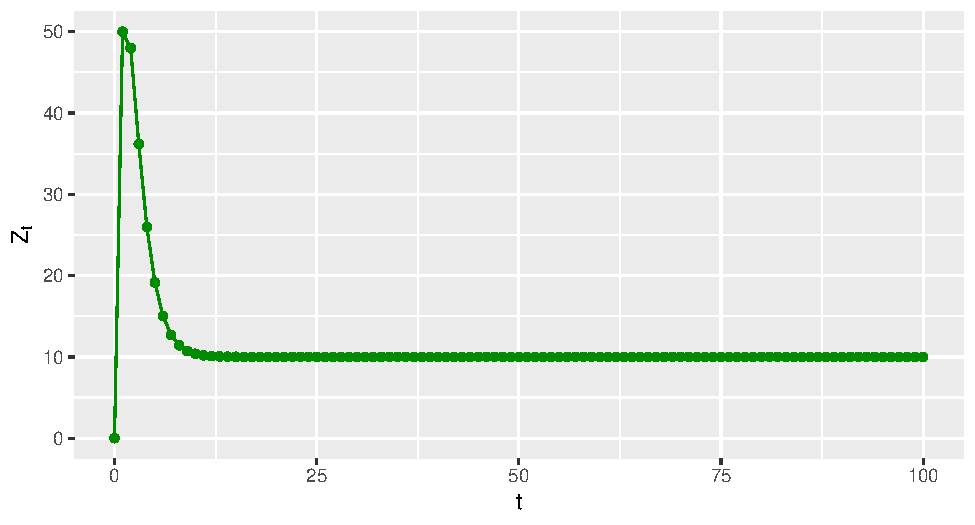
\includegraphics{Notas-Series-Tiempo_files/figure-latex/fig23-1} 

}

\caption{Evolución del proceso dado por $Z_t =3+0.9Z_{t-1}-0.2Z_{t-2}$}\label{fig:fig23}
\end{figure}

Finalmente, discutiremos la solución para las Ecuaciones Lineales en Diferencia de Orden \(p\), donde \(p \geq 2\). En general, una ecuación de este tipo se puede escribir como:
\begin{equation}
    Z_t = a_0 + a_1 Z_{t-1} + a_2 Z_{t-2} + \ldots + a_p Z_{t-p}
    \label{eq:EDOP}
\end{equation}

Donde \(t = \ldots, -2, -1, 0, 1, 2, \ldots\) y \(a_p \neq 0\). La ecuación \eqref{eq:EDOP} se puede escribir como:
\begin{eqnarray}
    Z_t - a_1 Z_{t-1} - a_2 Z_{t-2} - \ldots - a_p Z_{t-p} & = & a_0 \nonumber \\
    Z_t - a_1 L Z_t - a_2 L^2 Z_t - \ldots - a_p L^p Z_t & = & a_0 \nonumber \\
    (1 - a_1 L - a_2 L^2 - \ldots - a_p L^p) Z_t & = & a_0
    \label{eq:EDOP2}
\end{eqnarray}

Por el Teorema Fundamental del Álgebra es posible escribir la ecuación \eqref{eq:EDOP2} como:
\begin{eqnarray}
    (1 - g_1 L)(1 - g_1 L) \ldots (1 - g_p L) Z_t & = & a_0
    \label{eq:EDOP3}
\end{eqnarray}

Utilizando la ecuación \eqref{eq:EDOP2} y la ecuación \eqref{eq:EDOP3} tenemos que la solución general de una ecuación como la descrita en \eqref{eq:EDOP} se puede escribir como:
\begin{equation}
    Z_t  =  \frac{a_0}{1 - a_1 - a_2 - \ldots - a_p} + s_1 g^t_1 + s_2 g^t_2 + \ldots + s_p g^t_p \\
    \label{eq:EDOPGEN}
\end{equation}\\
\begin{eqnarray}
    Z_t & = & \frac{a_0}{(1 - g_1)(1 - g_1) \ldots (1 - g_p)} + s_1 g^t_1 + s_2 g^t_2 + \ldots + s_p g^t_p 
    \label{eq:EDOPGEN2}
\end{eqnarray}

Donde \(s_1\), \(s_2\), \ldots, \(s_p\) son constantes que se determinan utilizando \(p\) valores partículares de \(Z_t\), y la solución general descrita en las ecuaciones \eqref{eq:EDOPGEN} y \eqref{eq:EDOPGEN2} implica encontrar \(p\) raíces: \(x_1 = g^{-1}_1\), \(x_2 = g^{-1}_2\), \ldots, \(x_p = g^{-1}_p\) de los siguientes polinomios equivalentes:
\begin{eqnarray}
    (1 - g_1)(1 - g_1) \ldots (1 - g_p) = 0
    \label{eq:POLGEN1}
\end{eqnarray}

\begin{eqnarray}
    1 - a_1 x - a_2 x^2 - \ldots - a_p x^p = 0
    \label{eq:POLGEN2}
\end{eqnarray}

\begin{eqnarray}
    a_p x^p + \ldots + a_2 x^2 + a_1 x - 1 = 0
    \label{eq:POLGEN3}
\end{eqnarray}

Antes de plantear la solución general, analicemos una solución particular cuando un conjunto de las \(p\) raíces, digamos un total de \(m\), son iguales, es decir, cuando sucede que \(g_1 = g_2 = \ldots = g_m = g\) (con \(1 < m \leq p\)). En este caso la solución general en la ecuación \eqref{eq:EDOPGEN2} se escribe como:
\begin{eqnarray}
    Z_t & = & \frac{a_0}{(1 - g)^m(1 - g_{m+1}) \ldots (1 - g_p)} \nonumber \\ 
    & & + s_1 g^t + s_2 t g^t + \ldots + s_m t^{m-1} g^t + s_{m+1} g^t_{m+1} + \ldots + s_{p} g^t_{p}
    \label{eq:EDOPGEN3}
\end{eqnarray}

Definamos:
\begin{equation}
    f(g) = \frac{1}{1 - g} = \sum_{j = 0}^{\infty} g^j
    \label{eq:EDOPGEN4}
\end{equation}

Si retomamos el método descrito párrafos arriba tenemos las siguientes expresiones. Cuando \(m = 2\):
\begin{equation}
    f'(g) = \frac{1}{(1 - g)^2} = \sum_{j = 0}^{\infty} j g^{j-1} = \sum_{j = 0}^{\infty} (1 + j) g^j \nonumber
\end{equation}

En el otro extremo, cuando \(m = p\):
\begin{equation}
    f^{(p-1)}(g) = \frac{p-1}{(1 - g)^p} = \sum_{j = 0}^{\infty} \frac{(p-1+j)(p-2+j) \ldots (2+j)(1+j)}{(p-1)!} g^j
    \label{eq:EDOPGEN5}
\end{equation}

Así, en el extremo cuando \(m = p\) la solución general podría estar dada por:
\begin{eqnarray}
    Z_t & = & a_0 \sum_{j = 0}^{\infty} \frac{(p-1+j)(p-2+j) \ldots (2+j)(1+j)}{(p-1)!} g^j \nonumber \\
    & & + g^t \sum_{i = 0}^p s_i t^{i-1}
    \label{eq:EDOPGEN6}
\end{eqnarray}

Donde \(|{g} < 1|\), \(t = \ldots, -2, -1, 0, 1, 2, \ldots\). Para finalizar esta sección, plantearemos la expresión del polinomio característico que nos permitirá hacer el análisis de convergencia de los procesos. Partamos de que la ecuación \eqref{eq:POLGEN3} se puede escribir como:
\begin{equation}
    (x^{-1})^p - a_1 (x^{-1})^{p-1} - a_2 (x^{-1})^{p-1} - \ldots - a_p = 0
    \label{eq:POLGEN55}
\end{equation}

La ecuación \eqref{eq:POLGEN55} permite interpretar las raíces del polinomio característico de forma directa ya que \(x^{-1}_1 = g_1\), \(x^{-1}_2 = g_2\), \ldots, \(x^{-1}_p = g_p\). Así, siempre que \(p \geq 1\) en la ecuación \eqref{eq:EDOP}, diremos que el proceso descrito en esa ecuación dará como resultado un proceso convergente si se cumplen las dos condiciones \eqref{eq:COND1} y \eqref{eq:COND2}:
\begin{equation}
    |a_p| < 1  
    \label{eq:COND1}
\end{equation}
\begin{equation}
    a_1 + a_2 + \ldots + a_p < 1
    \label{eq:COND2}
\end{equation}

Alternativamente, cuando las raíces son reales, lo anterior es equivalente a la expresión \eqref{eq:COND3}:
\begin{eqnarray}
    |g_i| < 1
    \label{eq:COND3}
\end{eqnarray}

Para \(\forall i = 1, 2, \ldots, p\). Cuando las raíces son imaginarias, las dos condiciones \eqref{eq:COND1} y \eqref{eq:COND2} son equivalentes a la expresión \eqref{eq:COND4}:
\begin{eqnarray}
    \sqrt{g_i g_j} = \sqrt{u^2 + v^2} < 1 
    \label{eq:COND4}
\end{eqnarray}

Para \(\forall i \neq j\) y \(i, j = 1, 2, \ldots, p\). Cuando \(g_1 = g_2 = \ldots = g_p = g\), la condición de la ecuación \eqref{eq:COND3} se resume a que \(|g| < 1\). En resumen, las condiciones descritas en las ecuaciones \eqref{eq:COND3} y \eqref{eq:COND4} se puden ilustrar mediante un circulo unitario como el de la Figura \ref{fig:fig24} en que sí las raíces se ubican dentro de éste, podemos decir que el proceso es convergente en el largo plazo.

\begin{Shaded}
\begin{Highlighting}[]
\CommentTok{\# Crear datos para el círculo}
\NormalTok{theta }\OtherTok{\textless{}{-}} \FunctionTok{seq}\NormalTok{(}\DecValTok{0}\NormalTok{, }\DecValTok{2}\SpecialCharTok{*}\NormalTok{pi, }\AttributeTok{length.out=}\DecValTok{100}\NormalTok{)}
\NormalTok{x }\OtherTok{\textless{}{-}} \FunctionTok{cos}\NormalTok{(theta)}
\NormalTok{y }\OtherTok{\textless{}{-}} \FunctionTok{sin}\NormalTok{(theta)}
\NormalTok{circle\_data }\OtherTok{\textless{}{-}} \FunctionTok{data.frame}\NormalTok{(x, y)}

\CommentTok{\# Dibujar el círculo}
\FunctionTok{ggplot}\NormalTok{(circle\_data, }\FunctionTok{aes}\NormalTok{(}\AttributeTok{x=}\NormalTok{x, }\AttributeTok{y=}\NormalTok{y)) }\SpecialCharTok{+}
  \FunctionTok{geom\_polygon}\NormalTok{(}\AttributeTok{fill=}\ConstantTok{NA}\NormalTok{, }\AttributeTok{color=}\StringTok{"black"}\NormalTok{) }\SpecialCharTok{+}
  \FunctionTok{coord\_fixed}\NormalTok{(}\AttributeTok{ratio=}\DecValTok{1}\NormalTok{) }\SpecialCharTok{+}
  \FunctionTok{xlim}\NormalTok{(}\SpecialCharTok{{-}}\FloatTok{1.5}\NormalTok{, }\FloatTok{1.5}\NormalTok{) }\SpecialCharTok{+}
  \FunctionTok{ylim}\NormalTok{(}\SpecialCharTok{{-}}\FloatTok{1.5}\NormalTok{, }\FloatTok{1.5}\NormalTok{)}
\end{Highlighting}
\end{Shaded}

\begin{figure}

{\centering 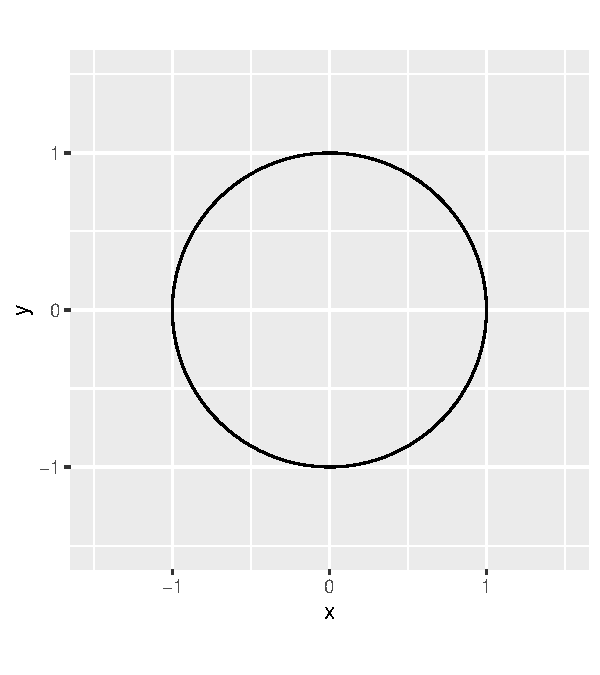
\includegraphics{Notas-Series-Tiempo_files/figure-latex/fig24-1} 

}

\caption{Circulo unitario en el que se cumple que $|g_i|<1$ y $(g_i g_j)^{1/2} = (u^2 + v^2)^{1/2} < 1$}\label{fig:fig24}
\end{figure}

\hypertarget{operador-de-rezago-l}{%
\section{Operador de rezago L}\label{operador-de-rezago-l}}

Denotemos, como se ha mencionado con anterioridad, con \(L\) al operador de rezago, el cual nos permitirá construir una relación entre diferencias y medias móviles como se verá más adelante en los procesos univariados \(AR(p)\), \(MA(q)\) y, en general, \(ARIMA(p, d, q)\). Sean \(X\), \(Y\) o \(Z\) variables con las que denotaremos a una serie de tiempo (note que hasta el momento no hemos definido qué es una serie de tiempo, no obstante, no es necesario definirla para hacer uso del operador).

En esta sección resumiremos algunas propiedades usadas en el capítulo y en capítulos más adelante. Así, si a dicha serie le aplicamos el operador rezago antes definido, el resultado deberá ser que cada uno de los valores de la serie es retardado o regresado un período. Es decir:

\begin{equation}
    L Z_t = Z_{t-1}
    \label{eq:Lag1}
\end{equation}

De esta forma, si aplicamos el operador rezago \(L\) a la nueva serie de tiempo dada por \(Z_{t-1}\) podemos obtener \(Z_{t-2}\). Haciendo uso de la ecuación \eqref{eq:Lag1} podemos obtener:
\begin{equation}
    L Z_{t-1} = L(L Z_t) = L^2 Z_t = Z_{t-2}
    \label{eq:Lag2}
\end{equation}

Mediante una generalización podemos obtener:
\begin{equation}
    L^k Z_t = Z_{t-k}
    \label{eq:Lag3}
\end{equation}

Para \(k = \ldots, -2, -1, 0, 1, 2, \ldots\). Así, para \(k = 0\) obtenemos la identidad dado que \(L^0 Z_t = Z_t\), de tal forma que siempre asumiremos que \(L^0 = 1\). En otro caso, cuando \(k > 0\) a la serie de tiempo a la cual se le aplique el operador rezago \(L\) se le deberá aplicar un rezago de \(k\) periodos a cada uno de los elementos de la serie. Por el contrario, cuando \(k < 0\) el operador rezago significa que se deberá adelantar \(|k|\) veces a cada elemento de la serie. Por ejemplo, \(L^{-3} Z_t = Z_{t+3}\).

Las reglas descritas en lo subsecuente se mantienen indistintamente cuando aplican para el caso de rezagar como para cuando se adelanta una serie. Como primera propiedad tomemos a la siguiente propiedad:
\begin{equation}
    L^{m} Z_{t-n} = L^{m} (L^{n} Z_{t}) = L^{m + n} Z_{t} = Z_{t-(n + m)} 
    \label{eq:Lag4}
\end{equation}

De lo anterior, podemos inferir el siguiente resultado:
\begin{equation}
    \Delta Z_{t} = Z_{t} - Z_{t-1} = (1 - L) Z_{t} 
    \label{eq:Lag5}
\end{equation}

En el caso de la diferencia de órden cuatro o cuarta diferencia se puede expresar como:
\begin{equation}
    \Delta_{4} Z_{t} = Z_{t} - Z_{t-4} = (1 - L^4) Z_{t}
\label{eq:Diff4}
\end{equation}

Al respecto, vale la pena aclarar que en ocasiones se hará uso de una notación alternativa dada por: \(\Delta^k\) o \(\Delta_k\), donde \(k = 1, 2, 3, \ldots\), indistintamente, ya que en ambos casos se referirá a una diferencia de orden \(k\). Esta notación resulta de gran utilidad cuando se quiere comparar períodos equivalentes como, por ejemplo, el mismo trimestre pero de un año anterior. De forma similar, para el caso de logaritmos podemos escribir la ecuación \eqref{eq:Diff4} como:
\begin{equation}
    \Delta^{4} ln(Z_{t}) = \Delta_{4} ln(Z_{t}) = ln(Z_{t}) - ln(Z_{t-4}) = (1 - L^4) ln(Z_{t}) 
    \label{eq:Diff5}
\end{equation}

Para el caso de una serie de tiempo que se le ha transformado mediante medias móviles, digamos de \(4\) periodos, podemos escribirla como:
\begin{equation}
    Zs_{t} = \frac{1}{4}(Z_{t} + Z_{t-1} + Z_{t-2} + Z_{t-3}) = \frac{1}{4}(1 + L + L^2 + L^3)Z_{t}
    \label{eq:Diff6}
\end{equation}

Una generalización del anterior caso puede ser escrita como un polinomio de orden \(p\) con el operador rezago \(L\) dado como:
\begin{eqnarray}
    \alpha(L) Z_{t} & = & (1 - \alpha_1 L - \alpha_2 L^2 - \ldots - \alpha_p L^p) Z_{t} \nonumber \\
    & = & Z_{t} - \alpha_1 Z_{t-1} - \alpha_2 Z_{t-2} - \ldots - \alpha_p Z_{t-p}
\label{eq:Ecp1}
\end{eqnarray}

Donde \(\alpha_i\) puede ser reemplazada por cualquier constante \(a_i\), con \(i = 1, 2, 3, \ldots\), para escribir ecuaciones como las anteriores. Adicionalmente, podemos decir que la ecuación \eqref{eq:Ecp1} es una generalización del caso de medias móviles, el cual admite una ponderación distinta para cada uno de los elementos rezagados.

Existe la posibilidad de operar más de un polinomio a la vez. Para múltiples polinomios (digamos, los polinomios \(\alpha(L)\) y \(\beta(L)\)) podemos escribir el siguiente resultado:
\begin{equation}
    \alpha(L) \beta(L) = \beta(L) \alpha(L)
    \label{eq:Diff7}
\end{equation}

Tales polinomios del operador rezago también son llamados \emph{filtros lineales}. A manera de ejemplo, tomemos el siguiente caso de diferencias para una serie de \(Z_t\):
\begin{equation}
    \Delta Z_{t} = (1 - L) Z_{t} = Z_{t} - Z_{t-1} 
    \label{eq:Diff8}
\end{equation}

y un proceso de medias móviles para la misma serie de \(Z_t\):
\begin{equation}
    Zs_{t} = \frac{1}{4}(1 + L^1 + L^2 + L^3) Z_{t} = \frac{1}{4}(Z_{t} + Z_{t-1} + Z_{t-2} + Z_{t-3}) 
    \label{eq:Diff9}
\end{equation}

De tal forma que el producto de ambos procesos se puede escribir como:
\begin{equation}
(1 - L) \times \frac{1}{4}(1 + L^1 + L^2 + L^3) Z_{t} = \frac{1}{4}(1 - L^4) Z_{t}
\label{eq:Diff10}
\end{equation}

Es decir, que el producto de dos polinomios, uno de diferencias y otro más de medias móviles, resulta en uno de diferencias pero de mayor grado, en este caso de grado 4.

\hypertarget{procesos-estacionarios-y-modelos-univariados}{%
\chapter{Procesos Estacionarios y Modelos Univariados}\label{procesos-estacionarios-y-modelos-univariados}}

\hypertarget{definiciuxf3n-de-ergodicidad-y-estacionariedad}{%
\section{Definición de ergodicidad y estacionariedad}\label{definiciuxf3n-de-ergodicidad-y-estacionariedad}}

A partir de esta sección introduciremos mayor formalidad matemática al análisis de las series de tiempo. Por ello cambiaremos un poco la notación y ocuparemos a \(X_t\) en lugar de \(Z_t\) como objeto de nuestro análisis. Con \(X_t\) denotaremos a una serie de tiempo, ya que con \(Z_t\) denotaremos a una variable, sin que ella fuera necesariamente una serie de tiempo en los términos que a continuación discutimos. Asimismo, iniciaremos por establecer una serie de definiciones.

De esta forma, definiremos a una \emph{serie de tiempo} como un vector de variables aleatorias de dimensión \(T\), dado como:
\begin{equation}
    X_1, X_2, X_3, \ldots ,X_T
    \label{eq:Serie0}
\end{equation}

Cada una de las \(X_t\) (\(t = 1, 2, \ldots, T\)) consideradas como una variable aleatoria. Así, también podemos denotar a la serie de tiempo como:
\begin{equation}
    \{ X_t \}^T_{t = 1}
    \label{eq:Serie}
\end{equation}

Es decir, definiremos a \emph{una serie de tiempo como una realización de un proceso estocástico} --o un Proceso Generador de Datos (PGD). Consideremos una muestra de los múltiples posibles resultados de muestras de tamaño \(T\), la colección dada por:
\begin{equation}
    \{X^{(1)}_1, X^{(1)}_2, \ldots, X^{(1)}_T\}
    \label{eq:Serie1}
\end{equation}

Digamos que la ecuación \eqref{eq:Serie1} es una de las tantas posibles resultantes del proceso estocástico o PGD. Eventualmente podríamos estar dispuestos a observar este proceso indefinidamente, de forma tal que estemos interesados en la secuencia dada por \(\{ X^{(1)}_t \}^{\infty}_{t = 1}\), lo cual no dejaría de ser sólo una de las tantas realizaciones o secuencias del proceso estocástico original.

Tan solo por poner un ejemplo, podríamos observar las siguientes realizaciones del mismo PGD:
\begin{eqnarray*}
    & \{X^{(2)}_1, X^{(2)}_2, \ldots, X^{(2)}_T\} & \\
    & \{X^{(3)}_1, X^{(3)}_2, \ldots, X^{(3)}_T\} & \\
    & \{X^{(4)}_1, X^{(4)}_2, \ldots, X^{(4)}_T\} & \\
    & \vdots & \\
    & \{X^{(j)}_1, X^{(j)}_2, \ldots, X^{(j)}_T\} & 
\end{eqnarray*}

Donde \(j \in \mathbb{Z}\). En lo subsecuente, diremos que una serie de tiempo es una realización del proceso estocástico subyacente. Considerando, en consecuencia, al proceso estocástico con todas sus posibilidades de realización.

Para hacer más sencilla la notación no distinguiremos entre el proceso en sí mismo y una de sus realizaciones, es decir, siempre escribiremos a una serie de tiempo como la secuencia mostrada en la ecuación \eqref{eq:Serie}, o más precisamente como la siguiente realización:
\begin{equation}
    \{ X_1, X_2, \ldots, X_T \}
    \label{eq:Serie2}
\end{equation}

O simplemente:
\begin{equation}
    X_1, X_2, \ldots, X_T
    \label{eq:Serie3}
\end{equation}

El proceso estocástico de dimensión \(T\) puede ser completamente descrito por su función de distribución multivariada de dimensión \(T\). No obstante, esto no resulta ser práctico cuando se opere más adelante en el curso. Por ello, en el curso y, en general, en casi todos los textos lo hacen, sólo nos enfocaremos en sus primero y segundo momentos. Es decir, en sus media o valor esperado:
\begin{equation*}
    \mathbb{E}[X_t]
\end{equation*}

Para \(t = 1, 2, \ldots, T\); o:
\begin{equation*}
\left[
    \begin{array}{c}
    \mathbb{E}[X_1] \\
    \mathbb{E}[X_2] \\
    \vdots \\
    \mathbb{E}[X_T]
    \end{array}
\right]
\end{equation*}

o,
\begin{equation*}
\left[
    \begin{array}{c}
    \mathbb{E}[X_1], \mathbb{E}[X_2], \ldots, \mathbb{E}[X_T]
    \end{array}
\right]
\end{equation*}

Y en su variaza:
\begin{equation*}
    Var[X_t] = \mathbb{E}[(X_t - \mathbb{E}[X_t])^2]
\end{equation*}

Para \(t = 1, 2, \ldots, T\), y de sus \(T(T-1)/2\) covarianzas:
\begin{equation*}
    Cov[X_t,X_s] = \mathbb{E}[(X_t - \mathbb{E}[X_t])(X_s - \mathbb{E}[X_s])]
\end{equation*}

Para \(t < s\). Por lo tanto, en la forma matricial podemos escribir lo siguiente:
\begin{equation*}
\left[
    \begin{array}{c c c c}
    Var[X_1] & Cov[X_1,X_2] & \cdots & Cov[X_1,X_T] \\
    Cov[X_2,X_1] & Var[X_2] & \cdots & Cov[X_2,X_T] \\
    \vdots & \vdots & \ddots & \vdots \\
    Cov[X_T,X_1] & Cov[X_T,X_2] & \cdots & Var[X_T] \\
    \end{array}
\right]
\end{equation*}

\begin{equation}
= \left[
    \begin{array}{c c c c}
    \sigma_1^2 & \rho_{12} & \cdots & \rho_{1T} \\
    \rho_{21} & \sigma_2^2 & \cdots & \rho_{2T} \\
    \vdots & \vdots & \ddots & \vdots \\
    \rho_{T1} & \rho_{T2} & \cdots & \sigma_T^2 \\
    \end{array}
\right]
    \label{eq:MATCOV}
\end{equation}

Donde es claro que en la matriz de la ecuación \eqref{eq:MATCOV} existen \(T(T-1)/2\) covarianzas distintas, ya que se cumple que \(Cov[X_t,X_s] = Cov[X_s,X_t]\), para \(t \neq s\).

A menudo, esas covarianzas son denominadas como autocovarianzas puesto que ellas son covarianzas entre variables aleatorias pertenecientes al mismo proceso estocástico pero en un momento \(t\) diferente. Si el proceso estocástico tiene una distribución normal multivariada, su función de distribución estará totalmente descrita por sus momentos de primer y segundo orden.

Ahora introduciremos el concepto de ergodicidad, el cual indica que los momentos muestrales, los cuales son calculados en la base de una serie de tiempo con un número finito de observaciones, en la medida que \(T \rightarrow \infty\) sus correspondientes momentos muestrales, tienden a los verdaderos valores poblacionales, los cuales definiremos como \(\mu\), para la media, y \(\sigma^2_X\) para la varianza.

Este concepto sólo es cierto si asumimos que, por ejemplo, el valor esperado y la varianza son como se dice a continuación para todo \(t = 1, 2, \ldots, T\):
\begin{eqnarray}
    \mathbb{E}[X_t] = \mu_t = \mu \\
    \label{eq:ESPERANZA}
\end{eqnarray}
\begin{eqnarray}
    Var[X_t] = \sigma^2_X
    \label{eq:VARIANZA}
\end{eqnarray}

Mas formalmente, se dice que el PGD o el proceso estocástico es ergódico en la media si:
\begin{equation}
    \displaystyle\lim_{T \to \infty}{\mathbb{E} \left[ \left( \frac{1}{T} \sum^{T}_{t = 1} (X_t - \mu) \right) ^2 \right]} = 0
    \label{eq:LIM1}
\end{equation}

y ergódico en la varianza si:
\begin{equation}
    \displaystyle\lim_{T \to \infty}{\mathbb{E} \left[ \left( \frac{1}{T} \sum^{T}_{t = 1} (X_t - \mu) ^2 - \sigma^2_X \right) ^2 \right]} = 0
    \label{eq:LIM2}
\end{equation}

Estas condiciones se les conoce como \emph{propiedades de consistencia} para las variables aleatorias. Sin embargo, éstas no pueden ser probadas. Por ello se les denomina como un supuesto que pueden cumplir algunas de las series. Más importante aún: \textbf{un proceso estocástico que tiende a estar en equilibrio estadístico en un orden ergódico, es estacionario}.

Podemos distinguir dos tipos de estacionariedad. Si asumimos que la función común de distribución del proceso estocástico no cambia a lo largo del tiempo, se dice que el proceso es \emph{estrictamente estacionario}. Como este concepto es difícil de aplicar en la práctica, solo consideraremos a la \emph{estacionariedad débil} o estacionariedad en sus momentos.

Definiremos a la estacionariedad por sus momentos del correspondiente proceso estocástico dado por \(\{X_t\}\):

\begin{enumerate}
\def\labelenumi{\arabic{enumi}.}
\item
  \emph{Estacionariedad en media}: Un proceso estocástico es estacionario en media si \(E[X_t] = \mu_t = \mu\) es constante para todo \(t\).
\item
  \emph{Estacionariedad en varianza}: Un proceso estocástico es estacionario en varianza si \(Var[X_t] = \mathbb{E}[(X_t - \mu_t)^2] = \sigma^2_X = \gamma(0)\) es constante y finita para todo \(t\).
\item
  \emph{Estacionariedad en covarianza}: Un proceso estocástico es estacionario en covarianza si \(Cov[X_t,X_s] = \mathbb{E}[(X_t - \mu_t)(X_s - \mu_s)] = \gamma(|s-t|)\) es sólo una función del tiempo y de la distancia entre las dos variables aleatorias. Por lo que no depende del tiempo denotado por \(t\) (no depende de la información contemporánea).
\item
  \emph{Estacionariedad débil}: Como la estacionariedad en varianza resulta de forma inmediata de la estacionariedad en covarianza cuando se asume que \(s = t\), un proceso estocástico es débilmente estacionario cuando es estacionario en media y covarianza.
\end{enumerate}

Puesto que resulta poco factible asumir una estacionariedad diferente a la débil, es adelante siempre que digamos que un proceso es estacionario se referirá al caso débil y sólo diremos que el proceso es estacionario, sin el apelativo de débil.

\textbf{Ejemplo}. Supongamos una serie de tiempo denotada por: \(\{U_t\}^T_{t = 0}\). Decimos que el proceso estocástico \(\{U_t\}\) es un \emph{proceso estocástico puramente aleatorio} o es un \emph{proceso estocástico de ruido blanco o caminata aleatoria}, si este tiene las siguientes propiedades:

\begin{enumerate}
\def\labelenumi{\arabic{enumi}.}
\item
  \(\mathbb{E}[U_t] = 0\), \(\forall t\);
\item
  \(Var[U_t] = \mathbb{E}[(U_t - \mu_t)^2] = \mathbb{E}[(U_t - \mu)^2] = \mathbb{E}[(U_t)^2] = \sigma^2\), \(\forall t\), y
\item
  \(Cov[U_t,U_s] = \mathbb{E}[(U_t - \mu_t)(U_s - \mu_s)] = \mathbb{E}[(U_t - \mu)(U_s - \mu)] = \mathbb{E}[U_t U_s] = 0\), \(\forall t \neq s\).
\end{enumerate}

En otras palabras, un proceso \(U_t\) es un ruido blanco si su valor esperado (promedio) es cero (0), tiene una varianza finita y constante, y además no le importa la historia pasada. Así, su valor presente no se ve influenciado por sus valores pasados, no importando respecto de qué período se tome referencia.

En apariencia, por sus propiedades, este proceso es débilmente estacionario --o simplemente, estacionario--. Todas las variables aleatorias tienen una media de cero, una varianza \(\sigma^2\) y no existe correlación entre ellas.

Ahora, supongamos que definimos un nuevo proceso estocástico \(\{X_t\}\) como:
\begin{equation}
    X_t = \left\{ \begin{array}{l} U_0  \mbox{ para } t = 0 \\ X_{t-1} + U_t \mbox{ para } t = 1, 2, 3, \ldots \end{array}\right.
    \label{eq:em1}
\end{equation}

Donde \(\{ U_t \}\) es un proceso puramente aleatorio. Este proceso estocástico, o caminata aleatoria sin tendencia (ajuste - drift), puede ser reescrito como:
\begin{equation}
    X_t = \sum^t_{j = 0} U_j
    \label{eq:em2}
\end{equation}

Tratemos de dar más claridad al ejemplo, para ello asumamos que generamos a \(\{U_t\}\) por medio del lanzamiento de una moneda. Donde obtenemos una cara (águila) con una probabilidad de \(0.5\), en cuyo caso decimos que la variable aleatoria \(U_t\) tomará el valor de \(+1\), y una cruz (sol) con una probabilidad de \(0.5\), en cuyo caso decimos que la variable aleatoria \(U_t\) toma el valor de \(-1\).

Este planteamiento cumple con las propiedades enunciadas ya que:

\begin{enumerate}
\def\labelenumi{\arabic{enumi}.}
\item
  \(\mathbb{E}[U_t] = 0.5 \times -1 + 0.5 \times 1 = 0\), \(\forall t\)
\item
  \(Var[U_t] = \mathbb{E}[(U_t - 0)^2] = \frac{1}{2}((-1)^2) + \frac{1}{2}((1)^2) = 1\), \(\forall t\)
\item
  \(Cov[U_t,U_s] = \mathbb{E}[(U_t - 0)(U_s - 0)] = \mathbb{E}[U_t \cdot U_s] = 0\), \(\forall t \neq s\).
\end{enumerate}

Retomando a nuestro proceso \(X_t\), diremos que el caso de \(X_0 = 0\), para \(t = 0\). Si verificamos cuáles son sus primeros y segundos momentos de \(\{X_t\}\), tenemos:
\begin{equation}
    \mathbb{E}[X_t] = \mathbb{E}\left[ \sum^t_{j=1} U_j \right] = \sum^t_{j=1} \mathbb{E}[U_j] = 0
    \label{eq:em3}
\end{equation}

En cuanto a la varianza:
\begin{eqnarray}
    Var[X_t] & = & Var \left[ \sum^t_{j=1} U_j \right] \nonumber \\
    & = & \sum^t_{j=1} Var[U_j] + 2 * \sum_{j \neq k} Cov[U_j,U_k] \nonumber \\
    & = & \sum^t_{j=1} 1 \nonumber \\
    & = & t
    \label{eq:em4}
\end{eqnarray}

Lo anterior, dado que hemos supuesto que en la caminata aleatoria todas las variables aleatorias son independientes, es decir, \(Cov[U_t,U_s] = E[U_t \cdot U_s] = 0\). Por su parte, la covarianza del proceso estocástico se puede ver como:
\begin{eqnarray*}
    Cov[X_t,X_s] & = & \mathbb{E} \left[ \left( \sum^t_{j=1} U_j - 0 \right) \left( \sum^s_{i=1} U_i - 0 \right) \right] \\
    & = & \mathbb{E}[(U_1 + U_2 + \ldots + U_t)(U_1 + U_2 + \ldots + U_s)] \\
    & = & \sum^t_{j=1} \sum^s_{i=1} \mathbb{E}[U_j U_i] \\
    & = & \mathbb{E}[U^2_1] + \mathbb{E}[U^2_2] + \ldots + \mathbb{E}[U^2_k] \\
    & = & \sigma^2 + \sigma^2 + \ldots + \sigma^2 \\
    & = & 1 + 1 + 1 + 1 \\
    & = & min(t,s)
\end{eqnarray*}

Así, el proceso estocástico dado por la caminata alaeatoria sin un término de ajuste es estacionario en media, pero no en varianza o en covarianza, y consecuentemente, en general no estacionario, condición que contraria al caso del proceso simple descrito en \(U_t\).

Es fácil ver que muchas de las posibilidades de realización de este proceso estocástico (series de tiempo) pueden tomar cualquiera de las rutas consideradas en la Figura \ref{fig:fig31}.

\begin{Shaded}
\begin{Highlighting}[]
\FunctionTok{set.seed}\NormalTok{(}\DecValTok{1234}\NormalTok{)}
\CommentTok{\# Utilizaremos una función guardada en un archivo a parte}
\CommentTok{\# Llamamos a la función:}
\FunctionTok{source}\NormalTok{(}\StringTok{"Caminata.R"}\NormalTok{)}

\CommentTok{\# Definimos argumentos de la función}
\NormalTok{Opciones }\OtherTok{\textless{}{-}} \FunctionTok{c}\NormalTok{(}\SpecialCharTok{{-}}\DecValTok{1}\NormalTok{, }\DecValTok{1}\NormalTok{)}
\CommentTok{\#}
\NormalTok{Soporte }\OtherTok{\textless{}{-}} \DecValTok{10000}

\CommentTok{\# Vamos a réplicar el proceso con estos parámetros}
\NormalTok{Rango }\OtherTok{\textless{}{-}} \DecValTok{200}
\CommentTok{\#}
\NormalTok{Caminos }\OtherTok{\textless{}{-}} \DecValTok{10}

\CommentTok{\#}

\ControlFlowTok{for}\NormalTok{(i }\ControlFlowTok{in} \DecValTok{1}\SpecialCharTok{:}\NormalTok{Caminos)\{}
\NormalTok{  TT }\OtherTok{\textless{}{-}} \FunctionTok{data.matrix}\NormalTok{(}\FunctionTok{data.frame}\NormalTok{(}\FunctionTok{Caminata}\NormalTok{(Opciones, Soporte)[}\DecValTok{1}\NormalTok{]))}
  \CommentTok{\#}
\NormalTok{  G\_t }\OtherTok{\textless{}{-}} \FunctionTok{data.matrix}\NormalTok{(}\FunctionTok{data.frame}\NormalTok{(}\FunctionTok{Caminata}\NormalTok{(Opciones, Soporte)[}\DecValTok{2}\NormalTok{]))}
  \CommentTok{\#}
  \FunctionTok{plot}\NormalTok{(TT, G\_t, }\AttributeTok{col =} \StringTok{"blue"}\NormalTok{, }\AttributeTok{type =} \StringTok{"l"}\NormalTok{, }\AttributeTok{ylab =} \StringTok{"Ganancias"}\NormalTok{, }
       \AttributeTok{xlab =} \StringTok{"Tiempo"}\NormalTok{, }\AttributeTok{ylim =} \FunctionTok{c}\NormalTok{(}\SpecialCharTok{{-}}\NormalTok{Rango,Rango))}
  \CommentTok{\#}
  \FunctionTok{par}\NormalTok{(}\AttributeTok{new =} \ConstantTok{TRUE}\NormalTok{)}
  \CommentTok{\#}
\NormalTok{  i }\OtherTok{\textless{}{-}}\NormalTok{ i }\SpecialCharTok{+}\DecValTok{1}
\NormalTok{\}}
\CommentTok{\#}
\FunctionTok{par}\NormalTok{(}\AttributeTok{new =} \ConstantTok{FALSE}\NormalTok{)}
\end{Highlighting}
\end{Shaded}

\begin{figure}

{\centering 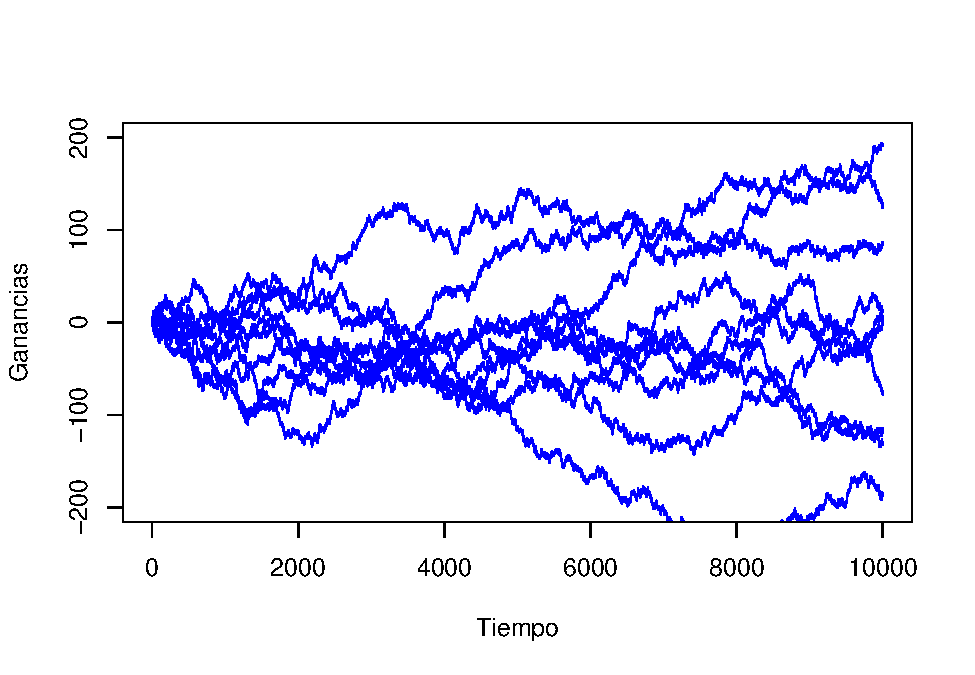
\includegraphics{Notas-Series-Tiempo_files/figure-latex/fig31-1} 

}

\caption{Ejemplo de 10 trayectorias de la caminata aleatoria, cuando sólo es posible cambios de +1 y -1}\label{fig:fig31}
\end{figure}

\hypertarget{funciuxf3n-de-autocorrelaciuxf3n}{%
\section{Función de autocorrelación}\label{funciuxf3n-de-autocorrelaciuxf3n}}

Para ampliar la discusión, es posible calcular la fuerza o intensidad de la dependencia de las variables aleatorias dentro de un proceso estocástico, ello mediante el uso de las autocovarianzas. Cuando las covarianzas son normalizadas respecto de la varianza, el resultado es un término que es independiente de las unidades de medida aplicadas, y se conoce como la \emph{función de autocorrelación}.

Para procesos estacionarios, dicha función de autocorrelación esta dada por:
\begin{equation}
    \rho(\tau) = \frac{\mathbb{E}[(X_t - \mu)(X_{t+\tau} - \mu)]}{\mathbb{E}[(X_t - \mu)^2]} = \frac{\gamma(\tau)}{\gamma(0)}
    \label{eq:em5}
\end{equation}

Donde \(\tau = \ldots, -2, -1, 0, 1, 2, \ldots\). Dicha función tiene las siguientes propiedades:

\begin{enumerate}
\def\labelenumi{\arabic{enumi}.}
\tightlist
\item
  \(\rho(0) = 1\). Es fácil demostrar que la función \(\rho(0)\) es:
\end{enumerate}

\begin{equation}
    \rho(0) = \frac{\mathbb{E}[(X_t - \mu)(X_{t + 0} - \mu)]}{\mathbb{E}[(X_t - \mu)^2]} = \frac{\mathbb{E}[(X_t - \mu)^2]}{\mathbb{E}[(X_t - \mu)^2]} = 1
\end{equation}

\begin{enumerate}
\def\labelenumi{\arabic{enumi}.}
\setcounter{enumi}{1}
\tightlist
\item
  \(\rho(\tau) = \rho(-\tau)\). Partiendo de la definción de \(\rho(\tau)\) podemos ver que la distancia que existe entre \(t\) y \(t + \tau\) es \(\tau\), de esta forma la autocorrelación de la variable \(X\) entre los periodos antes señalados debería ser la misma para el caso en que \(\rho(-\tau)\). Partamos de la ecuación para ver más claramente:
\end{enumerate}

\begin{equation}
    \rho(\tau) = \frac{\mathbb{E}[(X_t - \mu)(X_{t + \tau} - \mu)]}{\mathbb{E}[(X_t - \mu)^2]} = \frac{\mathbb{E}[(X_t - \mu)(X_{t - \tau} - \mu)]}{\mathbb{E}[(X_t - \mu)^2]} = \rho(-\tau)
\end{equation}

\begin{enumerate}
\def\labelenumi{\arabic{enumi}.}
\setcounter{enumi}{2}
\tightlist
\item
  \(\lvert\rho(\tau)\lvert \leq 1\), para todo \(\tau\).
\end{enumerate}

Derivado de las propiedades 1 y 2 antes descritas se puede concluir que sólo es necesario conocer la función de autocorrelación para el caso de \(\tau = 1, 2, 3, \ldots\), ya que de estos casos podemos derivar los valores de la función de autocorrelación complementarios de \(\tau = \ldots, -3, -2, -1\).

Partiendo de los supuestos de ergodicidad en relación a la media, varianza y covarianzas de un proceso estacionario, podemos estimar dichos parámetros con las siguientes formulaciones o propuestas de estimadores puntuales:
\begin{equation}
    \hat{\mu} = \frac{1}{T} \sum^T_{t=1} X_t
    \label{eq:em6}
\end{equation}

\begin{equation}
    \hat{\gamma}(0) = \frac{1}{T} \sum^T_{t=1} (X_t - \hat{\mu})^2 = \hat{\sigma}^2
    \label{eq:em7}
\end{equation}

\begin{equation}
    \hat{\gamma}(\tau) = \frac{1}{T} \sum^{T - \tau}_{t=1} (X_t - \hat{\mu})(X_{t+\tau} - \hat{\mu}) \mbox{, para } \tau = 1, 2, \ldots, T-1
    \label{eq:em8}
\end{equation}

No hacemos la demostración en estas notas --sería deseable que el alumno revisara la siguiente afirmación--, pero estos últimos son estimadores consistentes de \(\mu\), \(\gamma(0)\) y \(\gamma(\tau)\). Por su parte, un estimador consistente de la función de autocorrelación estará dado por:
\begin{equation}
  \hat{\rho}(\tau) = \frac{\sum^{T - \tau}_{t=1} (X_t - \hat{\mu})(X_{t+\tau} - \hat{\mu})}{\sum^T_{t=1} (X_t - \hat{\mu})^2} = \frac{\hat{\gamma}(\tau)}{\hat{\gamma}(0)}
  \label{eq:eqautocorr}
\end{equation}

El estimador de la ecuación \eqref{eq:eqautocorr} es asintóticamente insesgado. Por ejemplo, para el caso de un proceso de ruido blanco o caminata aleatoria, su varianza puede ser aproximada por el valor dado \(1/T\). Ésta tiene, asintóticamente, una distribución normal. Dado esto, el intervalo de confianza al \(95\%\) será el dado por \(\pm 2/\sqrt{T}\), en el cual se encuentra la mayoría de los coeficientes de autocorrelación estimados.

Ahora discutamos algunos ejemplos o aplicaciones. Cuando se realiza la evaluación de la estimación de un modelo de series de tiempo es importante saber si los residuales del modelo realmente tienen propiedades de un proceso puramente aleatorio, en particular, si ellos no están correlacionados entre sí. Así, la hipótesis a probar será:
\begin{equation}
    H_0 : \rho(\tau) = 0 \mbox{, para todo } \tau = 1, 2, \ldots, m \mbox{ y } m < T
    \label{eq:eqautocorr1}
\end{equation}

Esta expresión se puede interpretar como una prueba respecto de si la correlación entre la información de periodos atrás es cero con la información contemporánea. Para hacer una pruena global de la hipotésis de sí un número \(m\) de coeficientes de autocovarianzas son cero Box y Pierce (1970) desarrollarón la siguiente estadística:
\begin{equation}
    Q^* = T \sum_{j = 1}^{m} \hat{\rho} (j)^2
    \label{eq:eqautocorr2}
\end{equation}

Bajo la hipotésis nula esta estadística se distribulle asintóticamente como una chi cuadrado (\(\chi^2\)) con \(m-k\) grados de libertad y con \(k\) que representa al número de paramétros estimados.

Haciendo una aplicación estricta de la distribución de esta estadística, sabemos que esta se mantiene asintóticamente. Greta, Ljung y Box (1978) propusieron la siguiente modificación de la estadística para muestras pequeñas:
\begin{equation}
    Q = T(T + 2) \sum_{j = 1}^{m} \frac{\hat{\rho} (j)^2}{T - j}
    \label{eq:eqautocorr3}
\end{equation}

La cual también se distribulle asintóticamente como \(\chi^2\) con \(m-k\) grados de libertad.

También es intuitivamente claro que la hipótesis nula de no autocorrelación de residuales debería ser rechazada si alguno de los valores \(\hat{\rho} (j)\) es muy grande, es decir, si \(Q\) o \(Q^*\) es muy grande. O más precisamente, si estas estadísticas son más grandes que los correspondientes valores críticos de la distribución \(\chi^2\) con \(m-k\) grados de libertad a algún grado dado de signficancia.

Una alternativa para esta prueba es una del tipo Multiplicadores de Lagrange (o LM) desarrollada por Breusch (1978) y Godfrey (1978). La cual, al igual que las estadísticas \(Q\) y \(Q^*\), la hipotesis nula está dada por:

\begin{quote}
\(H_0\): Los residuales no están autocorrelacionados.
\end{quote}

\begin{quote}
\(H_a\): Los residuales muestran alguna acutocorrelación de forma autoregresiva o de medias móviles.
\end{quote}

La prueba consiste en realizar una regresión auxiliar en la cual los residuales se estiman en función de las variables explicativas del modelo original y en los residuales mismos pero rezagados hasta el término \(m\) (regresión auxiliar). La prueba resulta en una estadística con una distribución \(\chi^2\) con \(m\) grados de libertad la cual está dada por la expresión:
\begin{equation}
    LM = T \times R^2
    \label{eq:eqautocorr4}
\end{equation}

Donde \(R^2\) es el resultante de la regresión auxiliar y \(T\) es el número de observaciones totales.

En comparación con una prueba Durbin - Watson que es comúnmente usada en la econometría tradicional, para probar autocorrelación de los residuales, las estadísticas \(Q\), \(Q^*\) y \(LM\) tienen las siguientes ventajas:

\begin{enumerate}
\def\labelenumi{\arabic{enumi}.}
\item
  Permiten corroborar la existencia de autocorrelación para cualquier orden, y no solo para un primer orden (es decir, para cualquier valor de \(\tau = 1, 2, 3, \ldots\));
\item
  Los resultados se mantienen aún y cuando exista una probable variable endógena en forma rezagada, y
\item
  No depende del orden o la forma en que se acomoden las observaciones, algo que es muy probalble que ocurra en la econometría tradicional.
\end{enumerate}

El hecho de que los residuales no estén autocorrelacionados no implica que estos sean independientes y normalmente distribuidos. La ausencia de autocorrelación no implica una independencia estocástica si las variables son normalmente distribuidas.

A menudo se asume que estos residuales están distribuidos normalmente, ya que la mayoría de las pruebas estadísticas tienen este supuesto detrás. No obstante, ello también depende de los otros momentos de la distribución, específicamente del tercer y cuarto momento. Los cuales se expresan como:
\begin{equation*}
    \mathbb{E}[(X_t - \mathbb{E}[X_t])^i] \mbox{, } i = 3, 4
\end{equation*}

El tercer momento es necesario para determinar el sesgo, el cual está dado como:
\begin{equation}
    \hat{S} = \frac{1}{T} \frac{\sum_{t = 1}^{T} (X_t - \hat{\mu})^3}{\sqrt{\hat{\gamma}(0)^3}}
    \label{eq:eqautocorr6}
\end{equation}

Para distribuciones simétricas (como en el caso de la distribución normal) el valor teórico para el sesgo es cero.

La curtosis, la cual está dada en función del cuarto momento, se puede expresar como:
\begin{equation}
    \hat{K} = \frac{1}{T} \frac{\sum_{t = 1}^{T} (X_t - \hat{\mu})^4}{\hat{\gamma}(0)^2}
    \label{eq:eqautocorr7}
\end{equation}

Para el caso de una distribución normal, esta estadística toma el valor de 3. Valores más grandes que 3 indican que la distribución tiene colas anchas. En tales casos se ubican los datos financieros.

Usando el valor de las estadísticas para medir el sesgo y la curtosis, \(S\) y \(K\), respectivamente, Jarque y Bera (1980) propusieron una prueba de normalidad, la cual puede ser aplicada a series de tiempo en niveles o en diferencias indistintamente. Dicha prueba se expresa como:
\begin{equation}
    JB = \frac{T}{6} \left(\hat{S} + \frac{1}{4} (\hat{K} - 3)^2 \right) 
    \label{eq:eqautocorr8}
\end{equation}

La cual tiene una distribución \(\chi^2\) con \(2\) grados de libertad y donde \(T\) es el tamaño de la muestra. La hipótesis de que las observaciones están distribuidas de forma normal se rechaza si el valor de la estadística de prueba es más grande que los correspondientes valores críticos en tablas.

\textbf{Ejemplo}. Veamos un ejemplo para ilustrar el uso de la función de autocorrelación. Tomemos como variable al número de pasajeros transportados por el sistema de transporte del metro de la CDMX.\footnote{Los datos y algoritmo está disponible en el repositorio de GitHub y corresponde a la Clase 3.} Los datos empleados fueron tomados del INEGI y son una serie de tiempo en el período que va de enero de 2000 a mayo de 2023, es decir, 281 observaciones. Como se puede apreciar en la Figura \ref{fig:fig32}, el número de pasajeros por mes ha oscilado significativamente a lo largo del tiempo. Incluso podemos observar un cambio estructural de la serie entre 2011 y 2012. Asimismo, podemos ubicar una caída atípica que ocurrió en septiembre de 2017. Pero lo más relevante es la caída asociada a la pandemia de COVID-19 de 2020.

\begin{Shaded}
\begin{Highlighting}[]
\FunctionTok{library}\NormalTok{(ggplot2)}
\FunctionTok{library}\NormalTok{(dplyr)}
\FunctionTok{library}\NormalTok{(readxl)}

\NormalTok{Datos }\OtherTok{\textless{}{-}} \FunctionTok{read\_excel}\NormalTok{(}\StringTok{"BD/Base\_Transporte.xlsx"}\NormalTok{, }
                    \AttributeTok{sheet =} \StringTok{"Datos"}\NormalTok{, }\AttributeTok{col\_names =} \ConstantTok{TRUE}\NormalTok{)}

\FunctionTok{ggplot}\NormalTok{(}\AttributeTok{data =}\NormalTok{ Datos, }\FunctionTok{aes}\NormalTok{(}\AttributeTok{x =}\NormalTok{ Periodo, }\AttributeTok{y =}\NormalTok{ Pax\_Metro)) }\SpecialCharTok{+} 
  \FunctionTok{geom\_line}\NormalTok{(}\AttributeTok{linewidth =} \FloatTok{0.5}\NormalTok{, }\AttributeTok{color =} \StringTok{"darkblue"}\NormalTok{) }\SpecialCharTok{+}
  \CommentTok{\#geom\_point(size = 1.0, color = "darkblue") + }
  \CommentTok{\#theme\_bw() + }
  \FunctionTok{xlab}\NormalTok{(}\StringTok{"Tiempo"}\NormalTok{) }\SpecialCharTok{+} 
  \FunctionTok{ylab}\NormalTok{(}\StringTok{"Millones de pasajeros"}\NormalTok{) }\SpecialCharTok{+} 
  \FunctionTok{theme}\NormalTok{(}\AttributeTok{plot.title =} \FunctionTok{element\_text}\NormalTok{(}\AttributeTok{size =} \DecValTok{11}\NormalTok{, }\AttributeTok{face =} \StringTok{"bold"}\NormalTok{, }\AttributeTok{hjust =} \DecValTok{0}\NormalTok{)) }\SpecialCharTok{+} 
  \FunctionTok{theme}\NormalTok{(}\AttributeTok{plot.subtitle =} \FunctionTok{element\_text}\NormalTok{(}\AttributeTok{size =} \DecValTok{10}\NormalTok{, }\AttributeTok{hjust =} \DecValTok{0}\NormalTok{)) }\SpecialCharTok{+} 
  \FunctionTok{theme}\NormalTok{(}\AttributeTok{plot.caption =} \FunctionTok{element\_text}\NormalTok{(}\AttributeTok{size =} \DecValTok{10}\NormalTok{, }\AttributeTok{hjust =} \DecValTok{0}\NormalTok{)) }\SpecialCharTok{+}
  \FunctionTok{theme}\NormalTok{(}\AttributeTok{plot.margin =} \FunctionTok{unit}\NormalTok{(}\FunctionTok{c}\NormalTok{(}\DecValTok{1}\NormalTok{,}\DecValTok{1}\NormalTok{,}\DecValTok{1}\NormalTok{,}\DecValTok{1}\NormalTok{), }\StringTok{"cm"}\NormalTok{)) }\SpecialCharTok{+}
  \FunctionTok{labs}\NormalTok{(}
    \AttributeTok{title =} \StringTok{"Pasajeros Transportados en el Metro de la CDMX"}\NormalTok{,}
    \AttributeTok{subtitle =} \StringTok{"(Ene{-}2000 a Jul{-}2021)"}\NormalTok{,}
    \AttributeTok{caption =} \StringTok{"Fuente: Elaboración propia con información del INEGI, }\SpecialCharTok{\textbackslash{}n}\StringTok{https://www.inegi.org.mx/app/indicadores/?tm=0\&t=1090"}
\NormalTok{  )}
\end{Highlighting}
\end{Shaded}

\begin{figure}

{\centering 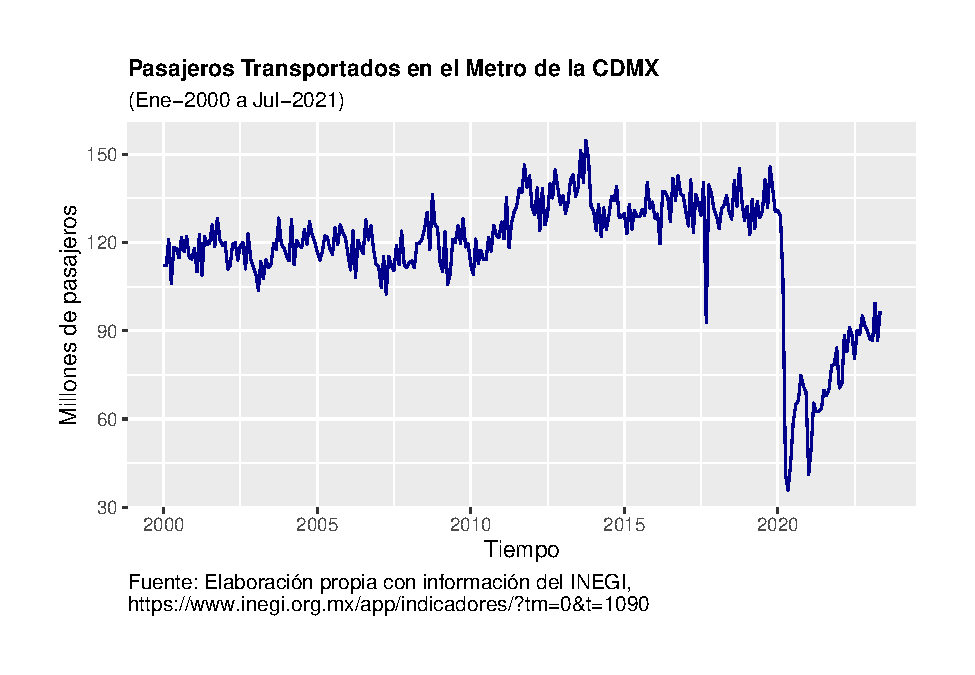
\includegraphics{Notas-Series-Tiempo_files/figure-latex/fig32-1} 

}

\caption{Evolución del número de pasajeros en el Metro de la CDMX, enero 2000 a mayo 2023}\label{fig:fig32}
\end{figure}

\begin{Shaded}
\begin{Highlighting}[]
\CommentTok{\#}
\FunctionTok{ggsave}\NormalTok{(}\StringTok{"Pax\_Metro.png"}\NormalTok{, }\AttributeTok{width =} \DecValTok{20}\NormalTok{, }\AttributeTok{height =} \DecValTok{15}\NormalTok{, }\AttributeTok{units =} \StringTok{"cm"}\NormalTok{)}
\end{Highlighting}
\end{Shaded}

A esta serie de tiempo le calculamos los pincipales estadísticos hasta ahora estudiados y obtenemos el Cuadro \ref{tab:foo}. En dicho cuadro se destaca que se muestra la función de autocirrelación para los tres primeros rezagos. Para mayor detalle, en la Figura \ref{fig:fig33} se muestra la función de autocorrelación, en donde las bandas descritas por las líneas azules son el intervalo de confianza dentro de las cuales no se puede rechazar la hipotésis nula de que \(H_0: \hat{\rho}(p) = 0\), para todo \(\tau = 1, 2, \ldots, T-1\).

\begin{longtable}[]{@{}
  >{\centering\arraybackslash}p{(\columnwidth - 2\tabcolsep) * \real{0.5000}}
  >{\centering\arraybackslash}p{(\columnwidth - 2\tabcolsep) * \real{0.5000}}@{}}
\caption{\label{tab:foo} Estadísticas descriptivas del número de pasajeros en el Metro de la CDMX, enero de 2000 a junio de 2019}\tabularnewline
\toprule\noalign{}
\begin{minipage}[b]{\linewidth}\centering
Estadística
\end{minipage} & \begin{minipage}[b]{\linewidth}\centering
Valor
\end{minipage} \\
\midrule\noalign{}
\endfirsthead
\toprule\noalign{}
\begin{minipage}[b]{\linewidth}\centering
Estadística
\end{minipage} & \begin{minipage}[b]{\linewidth}\centering
Valor
\end{minipage} \\
\midrule\noalign{}
\endhead
\bottomrule\noalign{}
\endlastfoot
\(\hat{\mu} = \frac{1}{T} \sum^T_{t=1} X_t\) & 124.3000 \\
\(\hat{\gamma}(0) = \frac{1}{T} \sum^T_{t=1} (X_t - \hat{\mu})^2\) & 103.6400 \\
\(\hat{\gamma}(1) = \frac{1}{T} \sum^{T - 1}_{t=1} (X_t - \hat{\mu})(X_{t+1} - \hat{\mu})\) & 63.1100 \\
\(\hat{\gamma}(2) = \frac{1}{T} \sum^{T - 2}_{t=1} (X_t - \hat{\mu})(X_{t+2} - \hat{\mu})\) & 72.9100 \\
\(\hat{\gamma}(3) = \frac{1}{T} \sum^{T - 3}_{t=1} (X_t - \hat{\mu})(X_{t+3} - \hat{\mu})\) & 63.6900 \\
\(\hat{\rho}(1) = \frac{\sum^{T - 1}_{t=1} (X_t - \hat{\mu})(X_{t+1} - \hat{\mu})}{\sum^T_{t=1} (X_t - \hat{\mu})^2} = \frac{\hat{\gamma}(1)}{\hat{\gamma}(0)}\) & 0.6089 \\
\(\hat{\rho}(2) = \frac{\sum^{T - 2}_{t=1} (X_t - \hat{\mu})(X_{t+2} - \hat{\mu})}{\sum^T_{t=1} (X_t - \hat{\mu})^2} = \frac{\hat{\gamma}(2)}{\hat{\gamma}(0)}\) & 0.7035 \\
\(\hat{\rho}(3) = \frac{\sum^{T - 3}_{t=1} (X_t - \hat{\mu})(X_{t+3} - \hat{\mu})}{\sum^T_{t=1} (X_t - \hat{\mu})^2} = \frac{\hat{\gamma}(3)}{\hat{\gamma}(0)}\) & 0.6145 \\
\(Q^* = T \sum_{j = 1}^{1} \hat{\rho} (j)^2\) & 86.7577 \\
\(Q^* = T \sum_{j = 1}^{2} \hat{\rho} (j)^2\) & 290.9279 \\
\end{longtable}

\begin{Shaded}
\begin{Highlighting}[]
\NormalTok{Pax\_Metro }\OtherTok{\textless{}{-}} \FunctionTok{ts}\NormalTok{(Datos}\SpecialCharTok{$}\NormalTok{Pax\_Metro, }
                \AttributeTok{start =} \DecValTok{2000}\NormalTok{, }
                \AttributeTok{freq =} \DecValTok{12}\NormalTok{)}

\FunctionTok{acf}\NormalTok{(Pax\_Metro, }
    \AttributeTok{lag.max =} \DecValTok{150}\NormalTok{, }
    \AttributeTok{xlab =} \StringTok{\textquotesingle{}Resagos k en meses\textquotesingle{}}\NormalTok{, }
    \AttributeTok{main =} \StringTok{"Funcion de Autocorrelación del número de pasajeros del metro"}\NormalTok{)}
\end{Highlighting}
\end{Shaded}

\begin{figure}

{\centering 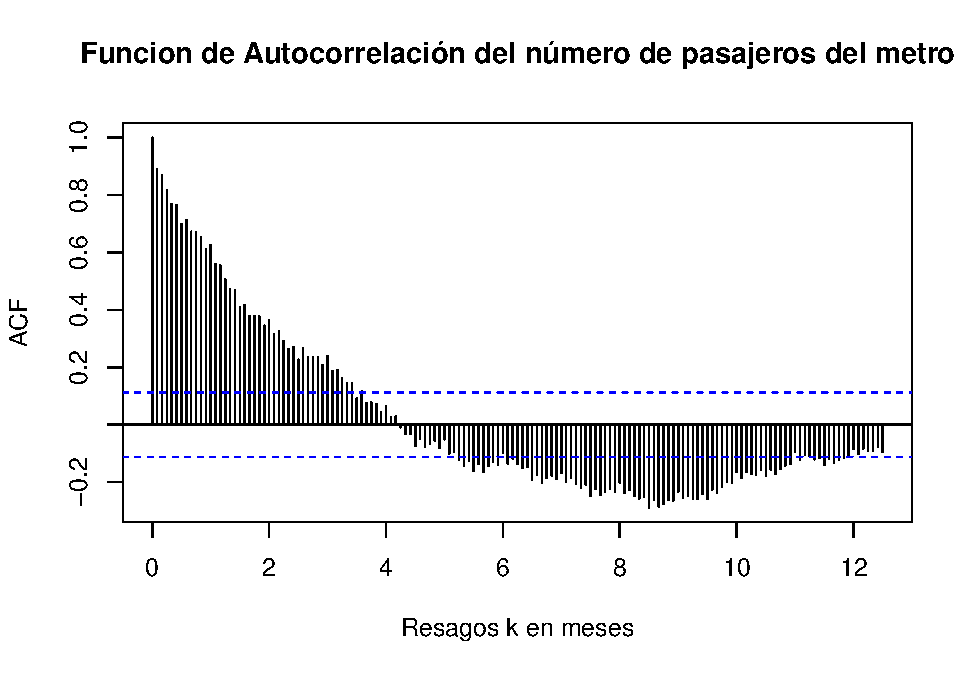
\includegraphics{Notas-Series-Tiempo_files/figure-latex/fig33-1} 

}

\caption{Función de Autocorrelación: 150 rezagos del número de pasajeros en el Metro de la CDMX, enero de 2000 a mayo de 2023}\label{fig:fig33}
\end{figure}

\hypertarget{procesos-estacionarios-univariados}{%
\section{Procesos estacionarios univariados}\label{procesos-estacionarios-univariados}}

En este capítulo analizaremos el método o metodología de análisis de series de tiempo propuesto por Box y Jenkins (1970). Los modelos
propuestos dentro de esta metodología o conjunto de métodos se han vuelto indispensables para efectos de realizar pronósticos de corto
plazo.

En este sentido, se analizarán los métodos más importantes en series de tiempo: procesos autoregresivos (AR, por sus siglas en inglés) y procesos de medias móviles (MA, por sus siglas en inglés). Asimismo, se realizará un análisis de los procesos que resultan de la combinación de ambos, conocida como ARMA, los cuales son más comúnmente usados para realizar pronósticos.

\hypertarget{procesos-autoregresivos-ar}{%
\section{Procesos Autoregresivos (AR)}\label{procesos-autoregresivos-ar}}

Los procesos autoregresivos tienen su origen en el trabajo de Cochrane y Orcutt de 1949, mediante el cual analizaron los residuales de una regresión clásica como un proceso autoregresivo. Puede consultarse el apéndice para la discusión del modelo de regresión clásica.

\hypertarget{ar1}{%
\subsection{AR(1)}\label{ar1}}

Como primer caso analizaremos al proceso autoregresivo de primer orden, \(AR(1)\), el cual podemos definir como una Ecuación Lineal en Diferencia de Primer Orden Estocástica. Diremos que una Ecuación Lineal en Diferencia de Primer Orden es estocástica si en su representación analítica considera un componente estocástico como en la ecuación \eqref{eq:EDOEst} descrita a continuación:
\begin{equation}
    X_t = a_0 + a_1 X_{t-1} + U_t
    \label{eq:EDOEst}
\end{equation}

Donde \(a_0\) es un término constante, \(U_t\) es un proceso estacionario, con media cero (0), una varianza finita y constante (\(\sigma^2\)) y una covarianza que depende de la distancia entre \(t\) y cualquier \(t-s\) (\(\gamma_s\))--que no depende de los valores pasados o futuros de la variable--, \(X_0\) es el valor inicial del proceso \(X_t\). No obstante, en ocasiones vamos a asumir que la covarianza será cero (0), por lo que en esos casos tendremos un proceso puramente aleatorio. Considerando la ecuación \eqref{eq:EDOEst} y un proceso de sustitución sucesivo podemos establecer lo siguiente, empezando con \(X_1\):
\begin{eqnarray*}
    X_{1} & = & a_0 + a_1 X_{0} + U_{1}
\end{eqnarray*}

Para \(X_2\):
\begin{eqnarray*}
    X_{2} & = & a_0 + a_1 X_{1} + U_{2} \\
    & = & a_0 + a_1 (a_0 + a_1 X_{0} + U_{1}) + U_{2} \\
    & = & a_0 + a_1 a_0 + a_1^2 X_{0} + a_1 U_{1} + U_{2}
\end{eqnarray*}

Para \(X_3\):
\begin{eqnarray*}
    X_{3} & = & a_0 + \alpha X_{2} + U_{3} \\
    & = & a_0 + a_1 (a_0 + a_1 a_0 + a_1^2 X_{0} + a_1 U_{1} + U_{2}) + U_{3} \\
    & = & a_0 + a_1 a_0 + a_1^2 a_0 + a_1^3 X_{0} + a_1^2 U_{1} + a_1 U_{2} + U_{3}
\end{eqnarray*}

Así, para cualquier \(X_t\), \(t = 1, 2, 3, \ldots\), obtendríamos:
\begin{eqnarray}
    X_{t} & = & a_0 + a_1 X_{t - 1} + U_{t} \nonumber \\
    & = & a_0 + a_1 (a_0 + a_1 a_0 + a_1^2 a_0 + \ldots + a_1^{t-2} a_0 + a_1^{t-1} X_{0} \nonumber \\
    &   & + a_1^{t-2} U_{1} + \ldots + a_1 U_{t - 2} + U_{t - 1}) + U_{t} \nonumber \\
    & = & a_0 + a_1 a_0 + a_1^2 a_0 + a_1^3 a_0 + \ldots + a_1^{t-1} a_0 + a_1^{t} X_{0} \nonumber \\
    &   & + a_1^{t-1} U_{1} + \ldots a_1^2 U_{t - 2} + a_1 U_{t - 1} + U_{t} \nonumber \\
    & = & (1 + a_1 + a_1^2 + a_1^3 + \ldots + a_1^{t-1}) a_0 + a_1^{t} X_{0} \nonumber \\
    &   & + a_1^{t-1} U_{1} + \ldots + a_1^2 U_{t - 2} + a_1 U_{t - 1} + U_{t}  \nonumber\\
    & = & \frac{1 - a_1^t}{1 - a_1} a_0 + a_1^{t} X_{0} + \sum^{t-1}_{j = 0} a_1^{j} U_{t - j} 
    \label{eq:EDOSSol}
\end{eqnarray}

De esta forma en la ecuación \eqref{eq:EDOSSol} observamos un proceso que es explicado por dos partes: una que depende del tiempo y otra que depende de un proceso estocástico. Asimismo, debe notarse que la condición de convergencia es idéntica al caso de ecuaciones en diferencia estudiadas al inicio del curso: \$ \textbar a\_1\textbar{} \textless{} 1\$, por lo que cuando \(t \to \infty\), la expresión \eqref{eq:EDOSSol} será la siguiente:
\begin{equation}
    X_t = a_0 \frac{1}{1 - a_1} + \sum^{\infty}_{j = 0} a_1^{j} U_{t - j}
    \label{eq:EDOSLP}
\end{equation}

Así, desaparece la parte dependiente del tiempo y únicamente prevalece la parte que es dependiente del proceso estocástico. Esta es la solución de largo plazo del proceso \(AR(1)\), la cual depende del proceso estocástico. Notemos, además, que esta solución implica que la variable o la serie de tiempo \(X_t\) es también un proceso estocástico que hereda las propiedades de \(U_t\). Así, \(X_t\) es también un proceso estocástico estacionario, como demostraremos más adelante.

Observemos que la ecuación \eqref{eq:EDOSLP} se puede reescribir si consideramos la formulación que en la literatura se denomina como la descomposición de Wold, en la cual se define que es posible asumir que \(\psi_j = a_1^j\) y se considera el caso en el cual \$ \textbar a\_1\textbar{} \textless{} 1 \$. De esta forma tendremos que, por ejemplo, cuando:
\begin{equation*}
    \sum^{\infty}_{j = 0} \psi^2_j = \sum^{\infty}_{j = 0} a_1^{2j} = \frac{1}{1 - a_1^2} 
\end{equation*}

Alternativamente y de forma similar a las ecuaciones en diferencia estudiadas previamente, podemos escribir el proceso \(AR(1)\) mediante el uso del operador rezago como:
\begin{eqnarray}
    X_t & = & a_0 + a_1 L X_t + U_t \nonumber \\
    X_t - a_1 L X_t & = & a_0 + U_t \nonumber \\
    (1 - a_1 L) X_t & = & a_0 + U_t \nonumber \\
    X_t & = & \frac{a_0}{1 - a_1 L} + \frac{1}{1 - a_1 L} U_t
    \label{eq:AR01}
\end{eqnarray}

En esta última ecuación retomamos el siguiente término para reescribirlo como:
\begin{equation}
    \frac{1}{1 - a_1 L} = 1 + a_1 L + a_1^2 L^2 + a_1^3 L^3 + \ldots 
\end{equation}

Tomando este resultado para sustituirlo en la ecuación \eqref{eq:AR01}, obtenemos la siguiente expresión:
\begin{eqnarray}
    X_t & = & (1 + a_1 L + a_1^2 L^2 + a_1^3 L^3 + \ldots) a_0 + (1 + a_1 L + a_1^2 L^2 + a_1^3 L^3 + \ldots) U_t \nonumber \\
    & = & (1 + a_1 + a_1^2 + a_1^3 + \ldots) a_0 + U_t + a_1 U_{t-1} + a_1^2 U_{t-2} + a_1^3 U_{t-3} + \ldots \nonumber \\
    & = & \frac{a_0}{1 - a_1} + \sum^{\infty}_{j = 0} a_1^j U_{t-j}
    \label{eq:AR1Sol}
\end{eqnarray}

Donde la condición de convergencia y estabilidad del proceso descrito en esta ecuación es que \$ \textbar a\_1\textbar{} \textless{} 1 \$. Por lo que hemos demostrado que, mediante el uso del operador de rezago, es posible llegar al mismo resultado que obtuvimos mediante el procedimiento de sustituciones iterativas.

La ecuación \eqref{eq:AR1Sol} se puede interpretar como sigue. La solución o trayectoria de equilibrio de un AR(1) se divide en dos partes. La primera es una constante que depende de los valores de \(a_0\) y \(a_1\). La segunda parte es la suma ponderada de las desviaciones o errores observados y acumulados en el tiempo hasta el momento \(t\).

Ahora obtendremos los momentos que describen a la serie de tiempo cuando se trata de un proceso \(AR(1)\). Para ello debemos obtener la media, la varianza y las covarianzas de \(X_t\). Para los siguientes resultados debemos recordar y tener en mente que si \(U_t\) es un proceso puramente aleatorio, entonces:

\begin{enumerate}
\def\labelenumi{\arabic{enumi}.}
\item
  \(\mathbb{E}[U_t] = 0\) para todo \(t\)
\item
  \(Var[U_t] = \sigma^2\) para todo \(t\)
\item
  \(Cov[U_t, U_s] = 0\) para todo \(t \neq s\)
\end{enumerate}

Dicho lo anterior y partiendo de la ecuación \eqref{eq:AR1Sol}, el primer momento o valor esperado de la serie de tiempo será el siguiente:
\begin{eqnarray}
    \mathbb{E}[X_t] & = & \mathbb{E} \left[ \frac{a_0}{1 - a_1} + \sum^{\infty}_{j = 0} a_1^j U_{t-j} \right] \nonumber \\
    & = & \frac{a_0}{1 - a_1} + \sum^{\infty}_{j = 0} a_1^j \mathbb{E}[U_{t-j}] \nonumber \\
    & = & \frac{a_0}{1 - a_1} = \mu
    \label{eq:AR1m1}
\end{eqnarray}

Respecto de la varianza podemos escribir la siguiente expresión a partir de la ecuación \eqref{eq:AR1Sol}:
\begin{eqnarray}
    Var[X_t] & = & \mathbb{E}[(X_t - \mu)^2] \nonumber \\
    & = & \mathbb{E} \left[ \left( \frac{a_0}{1 - a_1} + \sum^{\infty}_{j = 0} a_1^j U_{t-j} - \frac{a_0}{1 - a_1} \right)^2 \right] \nonumber \\
    & = & \mathbb{E}[(U_{t} + a_1 U_{t-1} + a_1^2 U_{t-2} + a_1^3 U_{t-3} + \ldots)^2] \nonumber \\
    & = & \mathbb{E}[U^2_{t} + a_1^2 U^2_{t-1} + a_1^4 U^2_{t-2} + a_1^6 U^2_{t-3} + \ldots \nonumber \\
    &   & + 2 a_1 U_t U_{t-1} + 2 a_1^2 U_t U_{t-2} + \ldots] \nonumber \\
    & = & \mathbb{E}[U^2_{t}] + a_1^2 \mathbb{E}[U^2_{t-1}] + a_1^4 \mathbb{E}[U^2_{t-2}] + a_1^6 \mathbb{E}[U^2_{t-3}] + \ldots \nonumber \\
    & = & \sigma^2 + a_1^2 \sigma^2 + a_1^4 \sigma^2 + a_1^6 \sigma^2 + \ldots \nonumber \\
    & = & \sigma^2 (1 + a_1^2 + a_1^4 + a_1^6 + \ldots) \nonumber \\
    & = & \sigma^2 \frac{1}{1 - a_1^2} = \gamma(0)
    \label{eq:AR1Var}
\end{eqnarray}

Previo a analizar la covarianza de la serie de tiempo, recordemos que para el proceso puramente aleatorio \(U_t\) su varianza y covarianza puede verse como \(\mathbb{E}[U_t, U_s] = \sigma^2\), para \(t = s\), y \(\mathbb{E}[U_t, U_s] = 0\), para cualquier otro caso, respectivamente.

Dicho lo anterior, partiendo de la ecuación \eqref{eq:AR1Sol} la covarianza de la serie estará dada por:
\begin{eqnarray}
    Cov(X_t, X_{t-\tau}) & = & \mathbb{E}[(X_t - \mu)(X_{t-\tau} - \mu)] \nonumber \\
    & = & \mathbb{E} \left[ \left( \frac{a_0}{1 - a_1} + \sum^{\infty}_{j = 0} a_1^j U_{t-j} - \frac{a_0}{1 - a_1} \right) \right. \nonumber \\
    &   & \left. \times \left( \frac{a_0}{1 - a_1} + \sum^{\infty}_{j = 0} a_1^j U_{t-\tau-j} - \frac{a_0}{1 - a_1} \right) \right] \nonumber \\
    & = & a_1^{\tau} \mathbb{E}[U^2_{t-\tau} + a_1 U^2_{t-\tau-1} + a_1^2 U^2_{t-\tau-2} + a_1^3 U^2_{t-\tau-3} + \ldots] \nonumber \\
    & = & a_1^{\tau} \sigma^2 \frac{1}{1 - a_1^2} = \gamma(\tau)
    \label{eq:AR1Cov}
\end{eqnarray}

Notése que con estos resultados en las ecuaciones \eqref{eq:AR1Var} y \eqref{eq:AR1Cov} podemos construir la función de autocorrelación
teórica como sigue:
\begin{eqnarray}
    \rho(\tau) & = & \frac{\gamma(\tau)}{\gamma(0)} \nonumber \\
    & = & a_1^\tau
\end{eqnarray}

Donde \(\tau = 1, 2, 3, \ldots\) y \$ \textbar a\_1\textbar{} \textless{} 1 \$. Este último resultado significa que cuando el proceso autoregresivo es de orden 1 (es decir, AR(1)) la función de autocorrelación teóricamente es igual al parámetro \(a_1\) elevado al número de rezagos considerados. No obstante, note que esto no significa que la autocorrelación observada sea como lo expresa en el planteamiento anterior. Por el contrario, una observación sencilla mostraría que la autocorrelación observada sería ligeramente distinta a la autocorrelación teórica. Ahora veamos algunos ejemplos.

\textbf{Ejemplo}. En el primer ejemplo simularemos una serie y mostraremos el análisis de un proceso construido considerando un proceso puramente aleatorio como componente \(U_t\). Por su parte, en un segundo ejemplo aplicaremos el análisis a una serie de tiempo de una variable económica observada.

Para el primer ejemplo, consideremos un proceso dado por la forma de un \(AR(1)\) como en la ecuación \eqref{eq:AR01} cuya solución está dada por la ecuación \eqref{eq:AR1Sol}. En específico, supongamos que el término o componente estocástico \(U_t\) es una serie generada a partir de números aleatorios de una función normal con media \(0\) y desviación estándar \(4\). Los detalles del proceso simulado se muestran en las siguientes gráficas.

La Figura \ref{fig:fig41} ilustra el comportamiento que se debería observar en una serie considerando el procedimiento iterativo de construcción. Por su parte, la Figura \ref{fig:fig42} ilustra el proceso o trayectoria de la solución de la serie de tiempo. Finalmente, las Figuras \ref{fig:fig43} y \ref{fig:fig44} muestran el correlograma calculado considerando una función de autocorrelación aplicada al porceso real y una función de autocorrelación aplicada al proceso teórico, respectivamente.

\begin{Shaded}
\begin{Highlighting}[]
\FunctionTok{library}\NormalTok{(ggplot2)}
\FunctionTok{library}\NormalTok{(dplyr)}
\FunctionTok{library}\NormalTok{(latex2exp)}

\NormalTok{a0 }\OtherTok{\textless{}{-}} \DecValTok{5}\NormalTok{; a1 }\OtherTok{\textless{}{-}} \FloatTok{0.9}\NormalTok{; X\_0 }\OtherTok{\textless{}{-}}\NormalTok{ (a0}\SpecialCharTok{/}\NormalTok{(}\DecValTok{1} \SpecialCharTok{{-}}\NormalTok{ a1)); T }\OtherTok{\textless{}{-}} \DecValTok{1000}

\NormalTok{X\_t }\OtherTok{\textless{}{-}} \FunctionTok{data.frame}\NormalTok{(}\AttributeTok{Tiempo =} \FunctionTok{c}\NormalTok{(}\DecValTok{0}\SpecialCharTok{:}\NormalTok{T))}


\FunctionTok{set.seed}\NormalTok{(}\DecValTok{12345}\NormalTok{)}

\CommentTok{\# Agregamos un término estocástico al data frame}

\NormalTok{X\_t}\SpecialCharTok{$}\NormalTok{U\_t }\OtherTok{\textless{}{-}} \FunctionTok{rnorm}\NormalTok{(T}\SpecialCharTok{+}\DecValTok{1}\NormalTok{, }\AttributeTok{mean =} \DecValTok{0}\NormalTok{, }\AttributeTok{sd =} \DecValTok{4}\NormalTok{)}

\CommentTok{\# Agregamos columnas con NA\textquotesingle{}s para un proceso teorico y uno real}
\NormalTok{X\_t}\SpecialCharTok{$}\NormalTok{X\_t }\OtherTok{\textless{}{-}} \ConstantTok{NA}
\NormalTok{X\_t}\SpecialCharTok{$}\NormalTok{XR\_t }\OtherTok{\textless{}{-}} \ConstantTok{NA}

\CommentTok{\# La serie teórica inicia en un valor inicial X\_0}
\NormalTok{X\_t}\SpecialCharTok{$}\NormalTok{X\_t[}\DecValTok{1}\NormalTok{] }\OtherTok{\textless{}{-}}\NormalTok{ X\_0}

\CommentTok{\# La serie real inicia en un valor inicial X\_0}
\NormalTok{X\_t}\SpecialCharTok{$}\NormalTok{XR\_t[}\DecValTok{1}\NormalTok{] }\OtherTok{\textless{}{-}}\NormalTok{ X\_0}

\CommentTok{\# Agregamos una columna para la función de Autocorrelación teórica:}
\NormalTok{X\_t}\SpecialCharTok{$}\NormalTok{rho }\OtherTok{\textless{}{-}}\ConstantTok{NA}

\ControlFlowTok{for}\NormalTok{ (i }\ControlFlowTok{in} \DecValTok{2}\SpecialCharTok{:}\NormalTok{(T }\SpecialCharTok{+} \DecValTok{1}\NormalTok{)) \{}
  \CommentTok{\# Real:}
\NormalTok{  X\_t}\SpecialCharTok{$}\NormalTok{XR\_t[i] }\OtherTok{=}\NormalTok{ a0 }\SpecialCharTok{+}\NormalTok{ a1}\SpecialCharTok{*}\NormalTok{X\_t}\SpecialCharTok{$}\NormalTok{XR\_t[i}\DecValTok{{-}1}\NormalTok{] }\SpecialCharTok{+}\NormalTok{ X\_t}\SpecialCharTok{$}\NormalTok{U\_t[i}\DecValTok{{-}1}\NormalTok{]}
  
  \CommentTok{\# Teórico:}
\NormalTok{  X\_t}\SpecialCharTok{$}\NormalTok{X\_t[i] }\OtherTok{=}\NormalTok{ X\_t}\SpecialCharTok{$}\NormalTok{X\_t[i}\DecValTok{{-}1}\NormalTok{] }\SpecialCharTok{+}\NormalTok{ (a1}\SpecialCharTok{\^{}}\NormalTok{(i}\DecValTok{{-}1}\NormalTok{))}\SpecialCharTok{*}\NormalTok{X\_t}\SpecialCharTok{$}\NormalTok{U\_t[i}\DecValTok{{-}1}\NormalTok{]}
  
  \CommentTok{\# Autocorrelación:}
\NormalTok{  X\_t}\SpecialCharTok{$}\NormalTok{rho[i}\DecValTok{{-}1}\NormalTok{] }\OtherTok{=}\NormalTok{ a1}\SpecialCharTok{\^{}}\NormalTok{(i}\DecValTok{{-}1}\NormalTok{)}
\NormalTok{\}}

\FunctionTok{ggplot}\NormalTok{(}\AttributeTok{data =}\NormalTok{ X\_t, }\FunctionTok{aes}\NormalTok{(}\AttributeTok{x =}\NormalTok{ Tiempo, }\AttributeTok{y =}\NormalTok{ XR\_t)) }\SpecialCharTok{+} 
  \FunctionTok{geom\_line}\NormalTok{(}\AttributeTok{size =} \FloatTok{0.5}\NormalTok{, }\AttributeTok{color =} \StringTok{"darkred"}\NormalTok{) }\SpecialCharTok{+}
  \CommentTok{\#theme\_bw() + }
  \FunctionTok{xlab}\NormalTok{(}\StringTok{"Tiempo"}\NormalTok{) }\SpecialCharTok{+} 
  \FunctionTok{ylab}\NormalTok{(}\FunctionTok{TeX}\NormalTok{(}\StringTok{"$X\_t$"}\NormalTok{)) }\SpecialCharTok{+} 
  \FunctionTok{theme}\NormalTok{(}\AttributeTok{plot.title =} \FunctionTok{element\_text}\NormalTok{(}\AttributeTok{size =} \DecValTok{11}\NormalTok{, }\AttributeTok{face =} \StringTok{"bold"}\NormalTok{, }
                                  \AttributeTok{hjust =} \DecValTok{0}\NormalTok{)) }\SpecialCharTok{+} 
  \FunctionTok{theme}\NormalTok{(}\AttributeTok{plot.subtitle =} \FunctionTok{element\_text}\NormalTok{(}\AttributeTok{size =} \DecValTok{10}\NormalTok{, }\AttributeTok{hjust =} \DecValTok{0}\NormalTok{)) }\SpecialCharTok{+} 
  \FunctionTok{theme}\NormalTok{(}\AttributeTok{plot.caption =} \FunctionTok{element\_text}\NormalTok{(}\AttributeTok{size =} \DecValTok{10}\NormalTok{, }\AttributeTok{hjust =} \DecValTok{0}\NormalTok{)) }\SpecialCharTok{+}
  \FunctionTok{theme}\NormalTok{(}\AttributeTok{plot.margin =} \FunctionTok{unit}\NormalTok{(}\FunctionTok{c}\NormalTok{(}\DecValTok{1}\NormalTok{,}\DecValTok{1}\NormalTok{,}\DecValTok{1}\NormalTok{,}\DecValTok{1}\NormalTok{), }\StringTok{"cm"}\NormalTok{)) }\SpecialCharTok{+}
  \FunctionTok{labs}\NormalTok{(}
    \AttributeTok{title =} \StringTok{"Comportamiento del Proceso Real (\textquotesingle{}Estimado\textquotesingle{})"}\NormalTok{,}
    \AttributeTok{subtitle =} \StringTok{"Con un error con Distribución Normal (media = 0, desviación estándar = 4)"}\NormalTok{,}
    \AttributeTok{caption =} \StringTok{"Fuente: Elaboración propia."}
\NormalTok{  )}
\end{Highlighting}
\end{Shaded}

\begin{figure}

{\centering 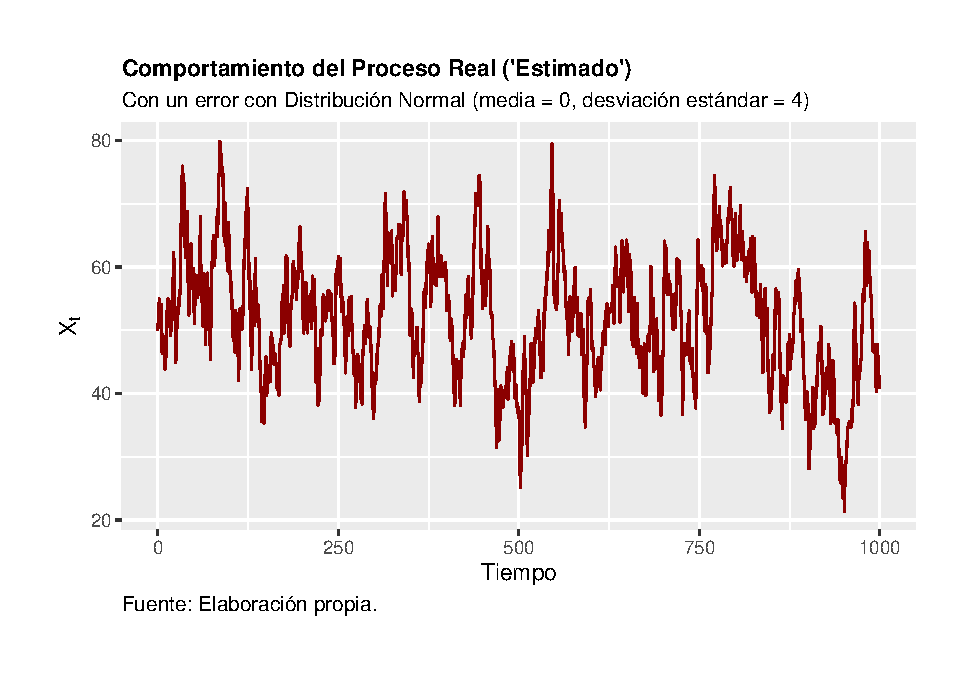
\includegraphics{Notas-Series-Tiempo_files/figure-latex/fig41-1} 

}

\caption{Comportamiento del Proceso Real ('Estimado')}\label{fig:fig41}
\end{figure}

\begin{Shaded}
\begin{Highlighting}[]
\FunctionTok{ggsave}\NormalTok{(}\StringTok{"G\_AR\_1\_Real.png"}\NormalTok{, }\AttributeTok{width =} \DecValTok{20}\NormalTok{, }\AttributeTok{height =} \DecValTok{10}\NormalTok{, }\AttributeTok{units =} \StringTok{"cm"}\NormalTok{)}
\end{Highlighting}
\end{Shaded}

\begin{Shaded}
\begin{Highlighting}[]
\FunctionTok{ggplot}\NormalTok{(}\AttributeTok{data =}\NormalTok{ X\_t, }\FunctionTok{aes}\NormalTok{(}\AttributeTok{x =}\NormalTok{ Tiempo, }\AttributeTok{y =}\NormalTok{ X\_t)) }\SpecialCharTok{+} 
  \FunctionTok{geom\_line}\NormalTok{(}\AttributeTok{size =} \FloatTok{0.5}\NormalTok{, }\AttributeTok{color =} \StringTok{"darkblue"}\NormalTok{) }\SpecialCharTok{+}
  \CommentTok{\#theme\_bw() + }
  \FunctionTok{xlab}\NormalTok{(}\StringTok{"Tiempo"}\NormalTok{) }\SpecialCharTok{+} 
  \FunctionTok{ylab}\NormalTok{(}\FunctionTok{TeX}\NormalTok{(}\StringTok{"$X\_t$"}\NormalTok{)) }\SpecialCharTok{+} 
  \FunctionTok{theme}\NormalTok{(}\AttributeTok{plot.title =} \FunctionTok{element\_text}\NormalTok{(}\AttributeTok{size =} \DecValTok{11}\NormalTok{, }\AttributeTok{face =} \StringTok{"bold"}\NormalTok{, }
                                  \AttributeTok{hjust =} \DecValTok{0}\NormalTok{)) }\SpecialCharTok{+} 
  \FunctionTok{theme}\NormalTok{(}\AttributeTok{plot.subtitle =} \FunctionTok{element\_text}\NormalTok{(}\AttributeTok{size =} \DecValTok{10}\NormalTok{, }\AttributeTok{hjust =} \DecValTok{0}\NormalTok{)) }\SpecialCharTok{+} 
  \FunctionTok{theme}\NormalTok{(}\AttributeTok{plot.caption =} \FunctionTok{element\_text}\NormalTok{(}\AttributeTok{size =} \DecValTok{10}\NormalTok{, }\AttributeTok{hjust =} \DecValTok{0}\NormalTok{)) }\SpecialCharTok{+}
  \FunctionTok{theme}\NormalTok{(}\AttributeTok{plot.margin =} \FunctionTok{unit}\NormalTok{(}\FunctionTok{c}\NormalTok{(}\DecValTok{1}\NormalTok{,}\DecValTok{1}\NormalTok{,}\DecValTok{1}\NormalTok{,}\DecValTok{1}\NormalTok{), }\StringTok{"cm"}\NormalTok{)) }\SpecialCharTok{+}
  \FunctionTok{labs}\NormalTok{(}
    \AttributeTok{title =} \StringTok{"Comportamiento del Proceso Teórico"}\NormalTok{,}
    \AttributeTok{subtitle =} \StringTok{"Con un error con Distribución Normal (media = 0, desviación estándar = 4)"}\NormalTok{,}
    \AttributeTok{caption =} \StringTok{"Fuente: Elaboración propia."}
\NormalTok{  )}
\end{Highlighting}
\end{Shaded}

\begin{figure}

{\centering 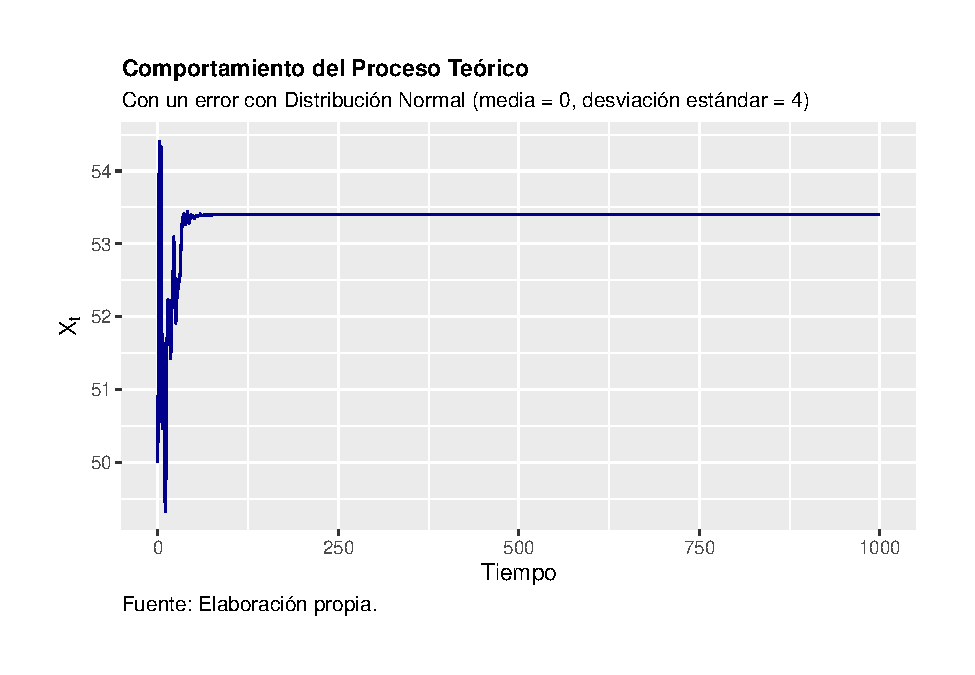
\includegraphics{Notas-Series-Tiempo_files/figure-latex/fig42-1} 

}

\caption{Comportamiento del Proceso Teórico}\label{fig:fig42}
\end{figure}

\begin{Shaded}
\begin{Highlighting}[]
\FunctionTok{ggsave}\NormalTok{(}\StringTok{"G\_AR\_1\_Teo.png"}\NormalTok{, }\AttributeTok{width =} \DecValTok{20}\NormalTok{, }\AttributeTok{height =} \DecValTok{10}\NormalTok{, }\AttributeTok{units =} \StringTok{"cm"}\NormalTok{)}
\end{Highlighting}
\end{Shaded}

\begin{Shaded}
\begin{Highlighting}[]
\FunctionTok{acf}\NormalTok{(X\_t}\SpecialCharTok{$}\NormalTok{XR\_t, }\AttributeTok{lag.max =} \DecValTok{30}\NormalTok{, }\AttributeTok{col =} \StringTok{"blue"}\NormalTok{, }
    \AttributeTok{ylab =} \StringTok{"Autocorrelacion"}\NormalTok{,}
    \AttributeTok{xlab=}\StringTok{"Rezagos"}\NormalTok{, }
    \AttributeTok{main=}\StringTok{"Funcion de Autocorrelacion Real"}\NormalTok{)}
\end{Highlighting}
\end{Shaded}

\begin{figure}

{\centering 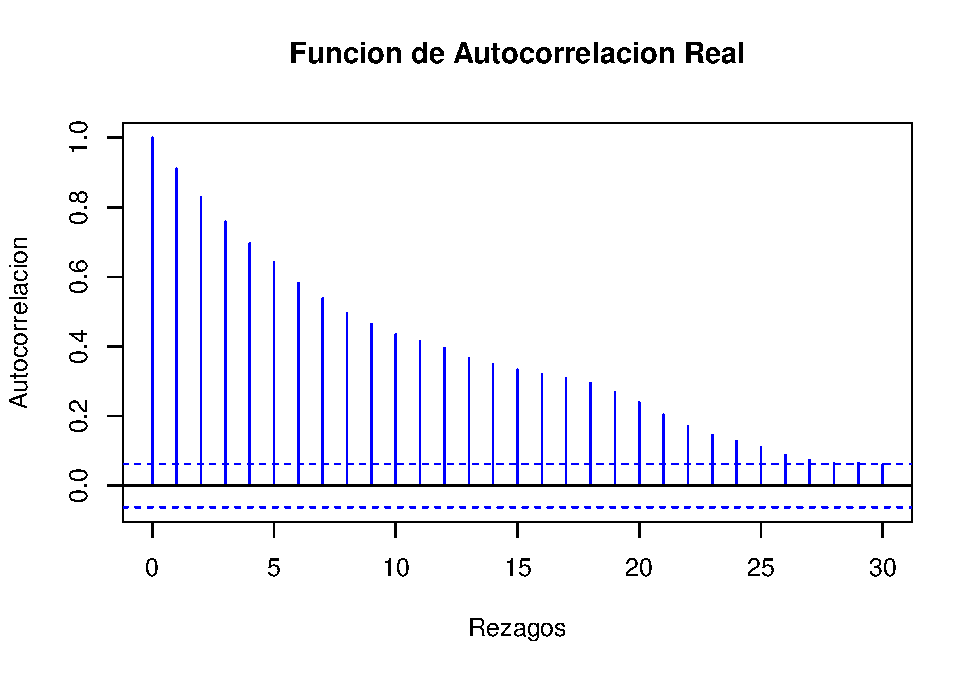
\includegraphics{Notas-Series-Tiempo_files/figure-latex/fig43-1} 

}

\caption{Funcion de Autocorrelacion Real}\label{fig:fig43}
\end{figure}

\begin{Shaded}
\begin{Highlighting}[]
\FunctionTok{barplot}\NormalTok{(X\_t}\SpecialCharTok{$}\NormalTok{rho[}\DecValTok{1}\SpecialCharTok{:}\DecValTok{30}\NormalTok{], }\AttributeTok{names.arg =} \FunctionTok{c}\NormalTok{(}\DecValTok{1}\SpecialCharTok{:}\DecValTok{30}\NormalTok{), }\AttributeTok{col =} \StringTok{"blue"}\NormalTok{, }
        \AttributeTok{border=}\StringTok{"blue"}\NormalTok{, }\AttributeTok{density =} \FunctionTok{c}\NormalTok{(}\DecValTok{10}\NormalTok{,}\DecValTok{20}\NormalTok{), }
        \AttributeTok{ylab =} \StringTok{"Autocorrelacion"}\NormalTok{, }
        \AttributeTok{xlab=}\StringTok{"Rezagos"}\NormalTok{, }
        \AttributeTok{main=}\StringTok{"Funcion de Autocorrelacion Teórica"}\NormalTok{)}
\end{Highlighting}
\end{Shaded}

\begin{figure}

{\centering 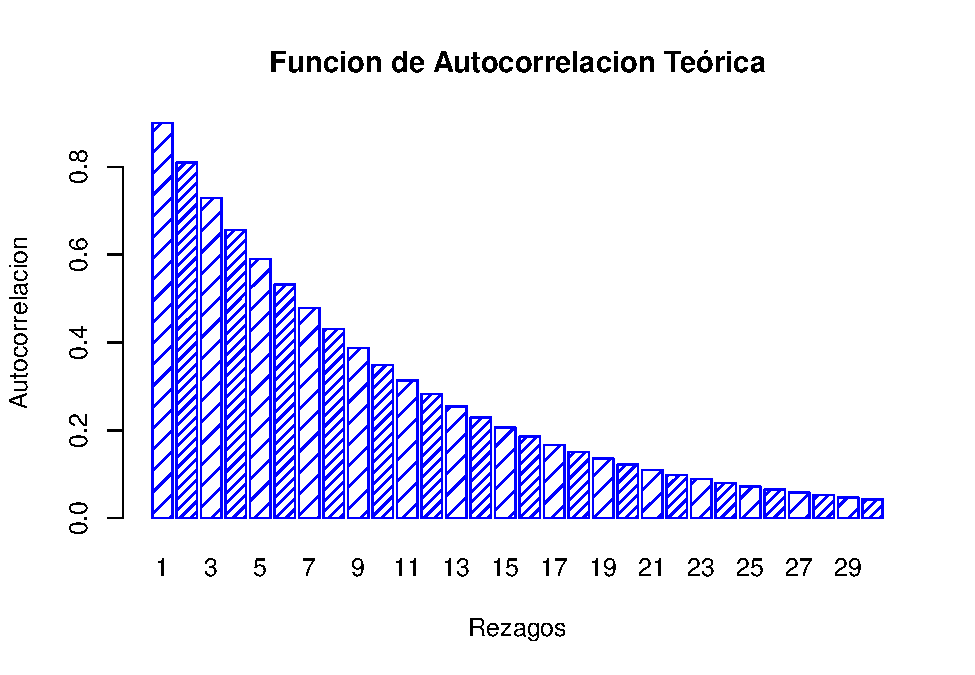
\includegraphics{Notas-Series-Tiempo_files/figure-latex/fig44-1} 

}

\caption{Funcion de Autocorrelacion Teórica}\label{fig:fig44}
\end{figure}

Recordemos que una trayectoria de equilibrio o solución de un \(AR(1)\) es como se muestra en la ecuación \eqref{eq:AR1Sol}. Así, nuestra serie simulada cumple con la característica de que los errores son más relevantes cuando la serie es corta. Por el contrario, los errores son menos relevantes, cuando la serie es muy larga. La Figura \ref{fig:fig45} ilustra esta observación de la trayectoria de equilibrio.

\begin{Shaded}
\begin{Highlighting}[]
\FunctionTok{ggplot}\NormalTok{(}\AttributeTok{data =}\NormalTok{ X\_t, }\FunctionTok{aes}\NormalTok{(}\AttributeTok{x =}\NormalTok{ Tiempo)) }\SpecialCharTok{+}
  \FunctionTok{geom\_line}\NormalTok{(}\FunctionTok{aes}\NormalTok{(}\AttributeTok{y =}\NormalTok{ XR\_t), }\AttributeTok{size =} \FloatTok{0.5}\NormalTok{, }\AttributeTok{color =} \StringTok{"darkred"}\NormalTok{) }\SpecialCharTok{+}
  \FunctionTok{geom\_line}\NormalTok{(}\FunctionTok{aes}\NormalTok{(}\AttributeTok{y =}\NormalTok{ X\_t), }\AttributeTok{size =} \FloatTok{0.5}\NormalTok{, }\AttributeTok{color =} \StringTok{"darkblue"}\NormalTok{) }\SpecialCharTok{+}
  \CommentTok{\#theme\_bw() + }
  \FunctionTok{xlab}\NormalTok{(}\StringTok{"Tiempo"}\NormalTok{) }\SpecialCharTok{+} 
  \FunctionTok{ylab}\NormalTok{(}\FunctionTok{TeX}\NormalTok{(}\StringTok{"$X\_t$"}\NormalTok{)) }\SpecialCharTok{+} 
  \FunctionTok{theme}\NormalTok{(}\AttributeTok{plot.title =} \FunctionTok{element\_text}\NormalTok{(}\AttributeTok{size =} \DecValTok{11}\NormalTok{, }\AttributeTok{face =} \StringTok{"bold"}\NormalTok{, }
                                  \AttributeTok{hjust =} \DecValTok{0}\NormalTok{)) }\SpecialCharTok{+} 
  \FunctionTok{theme}\NormalTok{(}\AttributeTok{plot.subtitle =} \FunctionTok{element\_text}\NormalTok{(}\AttributeTok{size =} \DecValTok{10}\NormalTok{, }\AttributeTok{hjust =} \DecValTok{0}\NormalTok{)) }\SpecialCharTok{+} 
  \FunctionTok{theme}\NormalTok{(}\AttributeTok{plot.caption =} \FunctionTok{element\_text}\NormalTok{(}\AttributeTok{size =} \DecValTok{10}\NormalTok{, }\AttributeTok{hjust =} \DecValTok{0}\NormalTok{)) }\SpecialCharTok{+}
  \FunctionTok{theme}\NormalTok{(}\AttributeTok{plot.margin =} \FunctionTok{unit}\NormalTok{(}\FunctionTok{c}\NormalTok{(}\DecValTok{1}\NormalTok{,}\DecValTok{1}\NormalTok{,}\DecValTok{1}\NormalTok{,}\DecValTok{1}\NormalTok{), }\StringTok{"cm"}\NormalTok{)) }\SpecialCharTok{+}
  \FunctionTok{labs}\NormalTok{(}
    \AttributeTok{title =} \StringTok{"Comportamiento de los Procesos Real y Teórico"}\NormalTok{,}
    \AttributeTok{subtitle =} \StringTok{"Con un error con Distribución Normal (media = 0, desviación estándar = 4)"}\NormalTok{,}
    \AttributeTok{caption =} \StringTok{"Fuente: Elaboración propia."}
\NormalTok{  )}
\end{Highlighting}
\end{Shaded}

\begin{figure}

{\centering 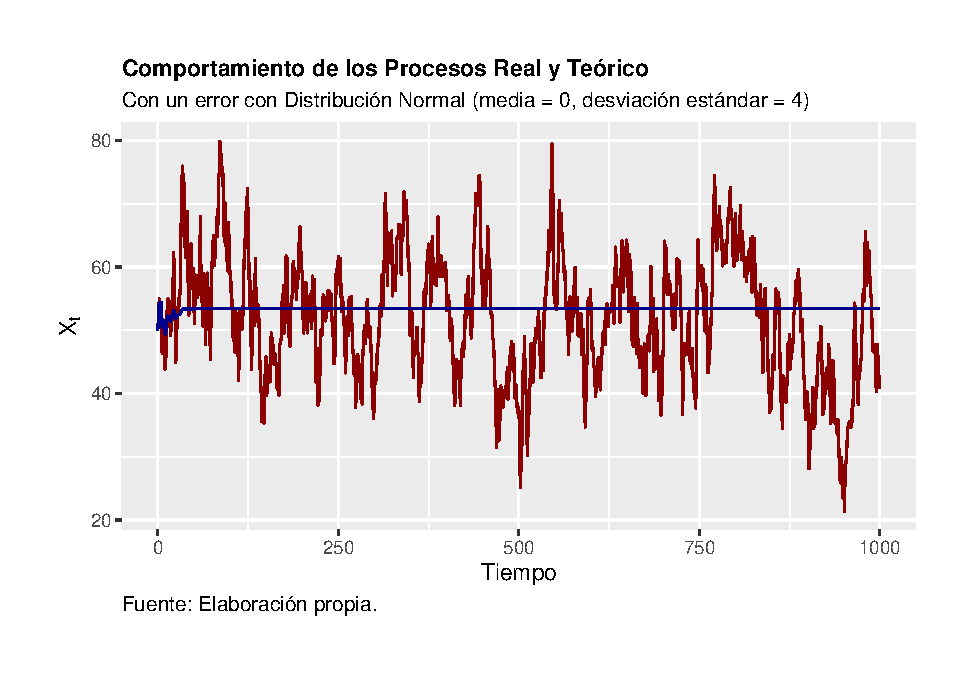
\includegraphics{Notas-Series-Tiempo_files/figure-latex/fig45-1} 

}

\caption{Comportamiento de los Procesos Real y Teórico}\label{fig:fig45}
\end{figure}

\begin{Shaded}
\begin{Highlighting}[]
\FunctionTok{ggsave}\NormalTok{(}\StringTok{"G\_AR\_1\_Comb.png"}\NormalTok{, }\AttributeTok{width =} \DecValTok{20}\NormalTok{, }\AttributeTok{height =} \DecValTok{10}\NormalTok{, }\AttributeTok{units =} \StringTok{"cm"}\NormalTok{)}
\end{Highlighting}
\end{Shaded}

\textbf{Ejemplo}. Para el segundo ejemplo consideremos una aplicación a una serie de tiempo en especifico: Pasajeros transportados mensualmente en el Sistema de Transporte Colectivo Metro (pasajeros medidos en millones).\footnote{Fuente: INEGI, \url{https://www.inegi.org.mx/app/indicadores/?tm=0&t=1090}.}

A la serie se le aplicará una metodología de estimación dada por el método de Máxima Verosimilitud (ML, por sus siglas en inglés). Antes de realizar el proceso de estimación, consideremos una transformación de diferencias logarítmicas con el objeto de obtener una serie de tiempo expresada en tasas de crecimiento\footnote{Estas tasas no son porcentuales, para hacerlas porcentuales faltaría multiplicar por 100 cada calor de la serie.} y con un comportamiento parecido a un proceso estacionario.

Así, para cada una de las series que analicemos en diferencias logarítmicas respecto del momento \(k\) las expresaremos bajo la siguiente transformación:
\begin{equation*}
    DLX_t = log(X_t) - log(X_{t-k})
\end{equation*}

Donde \(k = 1, 2, 3, \ldots\) y \(log(.)\) es la función logaritmo natural. Esta expresión se puede interpretar como una tasa de crecimiento, puesto que asumimos variaciones pequeñas para las cuales se cumple que: \(log(X_t) - log(X_{t-k}) \approx \frac{X_t - X_{t-k}}{X_t}\).

Primero, para realizar el análisis de una serie de tiempo deberemos decidir si éste se realizará para la serie en niveles o en diferencias. Por convención, decimos que la serie está en niveles si ésta se analiza sin hacerle ninguna transformación o si se analiza aplicando solo logaritmos. Cuando la serie se analiza en diferencias significa que la diferencia se hace sin aplicar logaritmos o aplicando logaritmos. Sin embargo, la convención es hacer un análisis en diferencias logarítmicas.

Para decidir cómo analizar la serie de pasajeros en el metro de la CDMX en la Figura \ref{fig:fig46} se muestra la gráfica de la serie en niveles (sin transformación logaritmica y con transformación logarítmica) y en diferencias logarítmicas mensuales (es decir, con \(k = 1\)).

\begin{Shaded}
\begin{Highlighting}[]
\FunctionTok{library}\NormalTok{(ggplot2)}
\FunctionTok{library}\NormalTok{(dplyr)}
\FunctionTok{library}\NormalTok{(readxl)}
\FunctionTok{library}\NormalTok{(stats)}

\NormalTok{Datos }\OtherTok{\textless{}{-}} \FunctionTok{read\_excel}\NormalTok{(}\StringTok{"BD/Base\_Transporte.xlsx"}\NormalTok{, }
                    \AttributeTok{sheet =} \StringTok{"Datos"}\NormalTok{, }\AttributeTok{col\_names =} \ConstantTok{TRUE}\NormalTok{)}

\CommentTok{\# En Niveles}
\NormalTok{Pax\_Metro }\OtherTok{\textless{}{-}} \FunctionTok{ts}\NormalTok{(Datos}\SpecialCharTok{$}\NormalTok{Pax\_Metro, }\AttributeTok{start =} \FunctionTok{c}\NormalTok{(}\DecValTok{2000}\NormalTok{, }\DecValTok{1}\NormalTok{), }
                \AttributeTok{freq =} \DecValTok{12}\NormalTok{)}

\CommentTok{\# En Logaritmos:}
\NormalTok{Pax\_LMetro }\OtherTok{\textless{}{-}} \FunctionTok{ts}\NormalTok{(}\FunctionTok{log}\NormalTok{(Datos}\SpecialCharTok{$}\NormalTok{Pax\_Metro), }\AttributeTok{start =} \FunctionTok{c}\NormalTok{(}\DecValTok{2000}\NormalTok{, }\DecValTok{1}\NormalTok{), }
                \AttributeTok{freq =} \DecValTok{12}\NormalTok{)}

\CommentTok{\# Diferencias mensuales:}
\NormalTok{Pax\_DLMetro }\OtherTok{\textless{}{-}} \FunctionTok{ts}\NormalTok{( }\FunctionTok{log}\NormalTok{(Datos}\SpecialCharTok{$}\NormalTok{Pax\_Metro) }\SpecialCharTok{{-}} 
                   \FunctionTok{lag}\NormalTok{( }\FunctionTok{log}\NormalTok{(Datos}\SpecialCharTok{$}\NormalTok{Pax\_Metro), }\DecValTok{1}\NormalTok{ ),}
                 \AttributeTok{start =} \FunctionTok{c}\NormalTok{(}\DecValTok{2000}\NormalTok{, }\DecValTok{1}\NormalTok{), }\AttributeTok{freq =} \DecValTok{12}\NormalTok{)}

\CommentTok{\#}
\FunctionTok{par}\NormalTok{(}\AttributeTok{mfrow =} \FunctionTok{c}\NormalTok{(}\DecValTok{3}\NormalTok{,}\DecValTok{1}\NormalTok{))}

\FunctionTok{plot}\NormalTok{(Pax\_Metro, }\AttributeTok{xlab =} \StringTok{"Tiempo"}\NormalTok{, }
     \AttributeTok{main =} \StringTok{"Pasajeros transportados (Millones) en el SCM"}\NormalTok{,}
     \AttributeTok{col =} \StringTok{"darkgreen"}\NormalTok{)}

\FunctionTok{plot}\NormalTok{(Pax\_LMetro, }\AttributeTok{xlab =} \StringTok{"Tiempo"}\NormalTok{, }
     \AttributeTok{main =} \StringTok{"LN Pasajeros transportados (Millones) en el SCM"}\NormalTok{,}
     \AttributeTok{col =} \StringTok{"darkblue"}\NormalTok{)}

\FunctionTok{plot}\NormalTok{(Pax\_DLMetro, }\AttributeTok{xlab =} \StringTok{"Tiempo"}\NormalTok{, }
     \AttributeTok{main =} \StringTok{"Diff LN Pasajeros transportados (Millones) en el SCM"}\NormalTok{, }
     \AttributeTok{col =} \StringTok{"darkred"}\NormalTok{)}
\end{Highlighting}
\end{Shaded}

\begin{figure}

{\centering 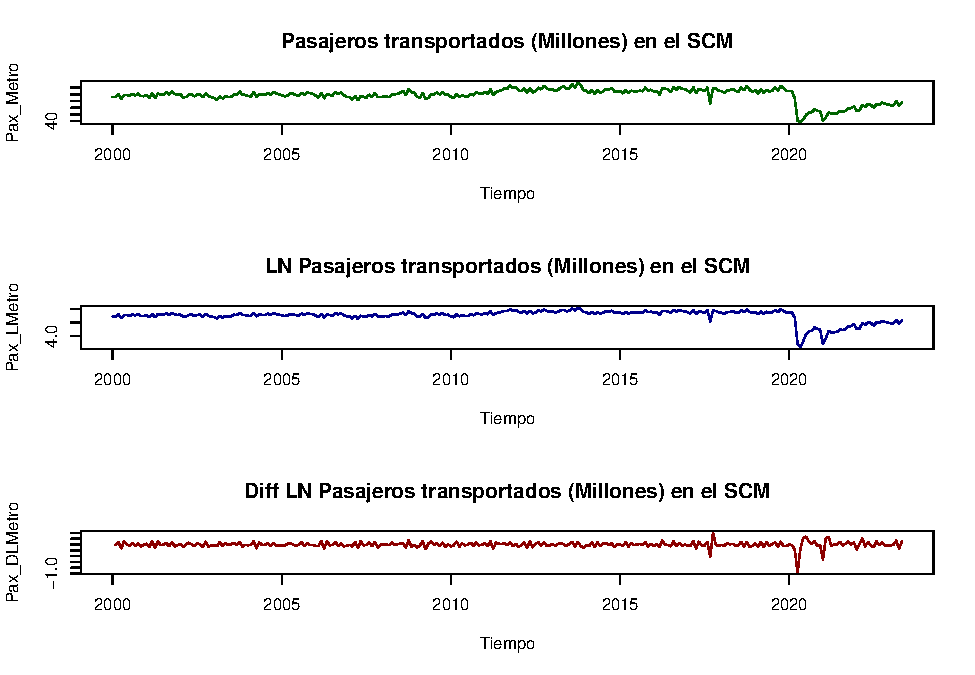
\includegraphics{Notas-Series-Tiempo_files/figure-latex/fig46-1} 

}

\caption{Pasajeros transportados (Millones) en el metro de la CDM en niveles y en diferencias logaritmicas}\label{fig:fig46}
\end{figure}

\begin{Shaded}
\begin{Highlighting}[]
\FunctionTok{par}\NormalTok{(}\AttributeTok{mfrow=}\FunctionTok{c}\NormalTok{(}\DecValTok{1}\NormalTok{,}\DecValTok{1}\NormalTok{))}
\end{Highlighting}
\end{Shaded}

A continuación, estimaremos una \(AR(1)\) para la serie en niveles bajo la transformación logarítmica (\(PaxLMetro_t\)) y en diferencias logarítmicas (\(PaxDLMetro_t\)). Para el primer caso, obtenemos el siguiente resultado:

\begin{longtable}[]{@{}cccccc@{}}
\caption{\label{tab:AR01} AR(1) para la variable \(PaxLMetro_t\).}\tabularnewline
\toprule\noalign{}
\endfirsthead
\endhead
\bottomrule\noalign{}
\endlastfoot
\(PaxLMetro_t\) & \(=\) & \(4.7419\) & \(+\) & \(0.5916\) & \(PaxLMetro_{t-1}\) \\
& & \((0.0105)\) & & \((0.0526)\) & \\
\(\hat{\sigma}^2\) & \(=\) & \(0.004335\) & \(AIC\) & \(=\) & \(-602.73\) \\
\end{longtable}

Para el segundo caso, obtenemos el siguiente resultado:

\begin{longtable}[]{@{}
  >{\centering\arraybackslash}p{(\columnwidth - 10\tabcolsep) * \real{0.1667}}
  >{\centering\arraybackslash}p{(\columnwidth - 10\tabcolsep) * \real{0.1667}}
  >{\centering\arraybackslash}p{(\columnwidth - 10\tabcolsep) * \real{0.1667}}
  >{\centering\arraybackslash}p{(\columnwidth - 10\tabcolsep) * \real{0.1667}}
  >{\centering\arraybackslash}p{(\columnwidth - 10\tabcolsep) * \real{0.1667}}
  >{\centering\arraybackslash}p{(\columnwidth - 10\tabcolsep) * \real{0.1667}}@{}}
\caption{\label{tab:AR0101} AR(1) para la variable \(PaxDLMetro_t\).}\tabularnewline
\toprule\noalign{}
\endfirsthead
\endhead
\bottomrule\noalign{}
\endlastfoot
\(PaxDLMetro_t\) & \(=\) & \(0.0007\) & \(-\) & \(0.6194\) & \(PaxDLMetro_{t-1}\) \\
& & \((0.0023)\) & & \((0.0511)\) & \\
\(\hat{\sigma}^2\) & \(=\) & \(0.003344\) & \(AIC\) & \(=\) & \(-660.53\) \\
\end{longtable}

En ambos casos observamos que el parámetro asociado al componente AR es significativo y cumple con la restricción de ser en valor absoluto menor a 1, por lo que la solución asociada al proceso será convergente. También en ambos casos se reporta la estadística o Criterio de Información de Akaike (AIC, por sus siglas en inglés), misma que más adelante discutiremos su importancia y aplicación.

\hypertarget{ar2}{%
\subsection{AR(2)}\label{ar2}}

Una vez analizado el caso de \(AR(1)\) analizaremos el caso del \(AR(2)\). La ecuación generalizada del proceso autoregresivo de orden 2 (denotado como \(AR(2)\)) puede ser escrita como:
\begin{equation}
    X_t = a_0 + a_1 X_{t-1} + a_2 X_{t-2} + U_t
    \label{eq:AR2Eq}
\end{equation}

Donde \(U_t\) denota un proceso puramente aleatorio con media cero (\(0\)), varianza constante (\(\sigma^2\)) y autocovarianza cero (\(Cov(U_t, U_s) = 0\), con \(t \neq s\)), y un parámetro \(a_2 \neq 0\). Así, utilizando el operador rezago podemos reescribir la ecuación
\eqref{eq:AR2Eq} como:
\begin{eqnarray*}     
    X_t - a_1 X_{t-1} - a_2 X_{t-2} & = & a_0 + U_t \\
    (1 - a_1 L^1 - a_2 L^2) X_t & = & a_0 + U_t
\end{eqnarray*}

Donde, vamos a denotar a \(\alpha (L) = (1 - a_1 L^1 - a_2 L^2)\), y lo denotaremos como un polinomio que depende del operador rezago y que es distinto de cero. De esta forma podemos reescribir la ecuación \eqref{eq:AR2Eq} como:
\begin{equation}
    \alpha(L) X_t = a_0 + U_t
\end{equation}

Ahora, supongamos que existe el inverso multiplicativo del polinomio \(\alpha(L)\), el cual será denotado como: \(\alpha^{-1}(L)\) y cumple con que:
\begin{equation}
    \alpha^{-1}(L) \alpha(L) = 1    
\end{equation}

Así, podemos escribir la solución a la ecuación \eqref{eq:AR2Eq} como:
\begin{equation*}
    X_t = \alpha^{-1}(L) \delta + \alpha^{-1}(L) U_t
\end{equation*}

Si utilizamos el hecho que \(\alpha^{-1}(L)\) se puede descomponer a través del procedimiento de Wold en un polinomio de forma similar al caso de \(AR(1)\), tenemos que:
\begin{equation}
    \alpha^{-1}(L) = \psi_0 + \psi_1 L + \psi_2 L^2 + \ldots
\end{equation}

Por lo tanto, el inverso multiplicativo \(\alpha^{-1}(L)\) se puede ver como:
\begin{equation}
    1 = (1 - a_1 L^1 - a_2 L^2) (\psi_0 + \psi_1 L + \psi_2 L^2 + \ldots)
    \label{eq:InvAlpha}
\end{equation}

Desarrollando la ecuación \eqref{eq:InvAlpha} tenemos la siguiente expresión:
\begin{eqnarray*}
  1 & = & \psi_0 + \psi_1 L + \psi_2 L^2 + \psi_3 L^3 + \ldots \\
  &  &  - a_1 \psi_0 L - a_1 \psi_1 L^2 - a_1 \psi_2 L^3 - \ldots \\
  &  &  - a_2 \psi_0 L^2 - a_2 \psi_1 L^3 - \ldots
\end{eqnarray*}

Ahora, podemos agrupar todos los términos en función del exponente asociado al operador rezago \(L\). La siguiente es una solución partícular y es una de las múltiples que podrían existir que cumpla con la ecuación \eqref{eq:InvAlpha}. Sin embargo, para efectos del análisis, sólo necesitamos una de esas soluciones. Utilizaremos las siguientes condiciones que deben cumplirse en una de las posibles soluciones:
\begin{eqnarray*}
  L^0 & : & \Rightarrow \psi_0 = 1 \\
  L^1 & : & \psi_1 - a_1 \psi_0 = 0 \Rightarrow \psi_1 = a_1 \\
  L^2 & : & \psi_2 - a_1 \psi_1 - a_2 \psi_0 = 0 \Rightarrow \psi_2 = a^2_1 + a_2 \\
  L^3 & : & \psi_3 - a_1 \psi_2 - a_2 \psi_1 = 0 \Rightarrow \psi_3 = a^3_1 + 2 a_1 a_2 \\
  & \vdots & 
\end{eqnarray*}

De esta forma podemos observar que en el límite siempre obtendremos una ecuación del tipo \(\psi_j - a_1 \psi_{j-1} - a_2 \psi_{j-2} = 0\) asociada a cada uno de los casos en que exista un \(L^j\), donde \(j \neq 0, 1\), y la cual siempre podremos resolver conociendo que las condiciones iniciales son: \(\psi_0 = 1\) y \(\psi_1 = a_1\).

Así, de las relaciones antes mencionadas y considerando que \(\alpha^{-1} (L)\) aplicada a una constante como \(a_0\), tendrá como resultado otra constante. De esta forma podemos escribir que la solución del proceso AR(2) en la ecuación \eqref{eq:AR2Eq} será dada por una expresión como sigue:
\begin{equation}
    X_t = \frac{a_0}{1 - a_1 - a_2} + \sum^{\infty}_{j = 0} \psi_{t - j} U_{t - j}
    \label{eq:AR2EqSol}
\end{equation}

Donde todos los parámetros \(\psi_i\) están determinados por los parámetros \(a_0\), \(a_1\) y \(a_2\). En particular, \(\psi_0 = 1\) y \(\psi_1 = a_1\), como describimos anteriormente. Al igual que en el caso del \(AR(1)\), en la ecuación \eqref{eq:AR2EqSol} las condiciones de estabilidad estarán dadas por las soluciones del siguiente polinomio característico:\footnote{Note que raíces son equivalentes al inversio de las del polinomio dado por $\lambda^2 a_2 - \lambda a_1 - 1 = 0$.}
\begin{equation}
    \lambda^2 - \lambda a_1 - a_2 = 0
\end{equation}

Así, la condición de estabilidad de la trayectoria es que \$ \textbar{} \lambda\_i \textbar{} \textless{} 1 \$, para \(i = 1, 2\). Es decir, es necesario que cada una de las raíces sea, en valor absoluto, siempre menor que la unidad. Estas son las condiciones de estabilidad para el proceso \(AR(2)\).

Finalmente, al igual que en un \(AR(1)\), a continuación determinamos los momentos de una serie que sigue un proceso \(AR(2)\). Iniciamos con la determinación de la media de la serie:
\begin{equation}
    \mathbb{E}[X_t] = \mu = \frac{a_0}{1 - a_1 - a_2}
\end{equation}

Lo anterior es cierto puesto que \(\mathbb{E}[U_{t - i}] = 0\), para todo \(i = 0, 1, 2, \ldots\). Para determinar la varianza utilizaremos las siguientes relaciones basadas en el uso del valor esperado, varianza y covarianza de la serie. Adicionalmente, para simplificar el trabajo asumamos que \(a_0 = 0\), lo cual implica que \(\mu = 0\). Dicho lo anterior, partamos de:
\begin{eqnarray*}
    \mathbb{E}[X_t X_{t - \tau}] & = & \mathbb{E}[(a_1 X_{t-1} + a_2 X_{t-2} + U_t) X_{t - \tau}]\\
    & = & a_1 \mathbb{E}[X_{t - 1} X_{t - \tau}] + a_2 \mathbb{E}[X_{t - 2} X_{t - \tau}] + \mathbb{E}[U_{t} X_{t - \tau}]
\end{eqnarray*}

Donde \(\tau = 0, 1, 2, 3, \ldots\) y \(\mathbb{E}[U_{t} X_{t - \tau}] = 0\) para todo \(\tau \neq 0\).\footnote{ Es fácil demostrar está afirmación, sólo requiere de desarrollar la expresión y utilizar el hecho de que $U_t$ es un proceso pueramente aleatorio, por lo que la covarianza es cero (0).} Dicho esto, podemos derivar el valor del valor esperado para diferentes valores de \(\tau\):
\begin{eqnarray*}
    \tau = 0 & : & \gamma(0) = \alpha_1 \gamma(1) + \alpha_2 \gamma(2) + \sigma^2 \\
    \tau = 1 & : & \gamma(1) = \alpha_1 \gamma(0) + \alpha_2 \gamma(1) \\
    \tau = 2 & : & \gamma(2) = \alpha_1 \gamma(1) + \alpha_2 \gamma(0) \\
    & \vdots & 
\end{eqnarray*}

Donde debe ser claro que \(\mathbb{E}[(X_{t} - \mu)(X_{t - \tau} - \mu)] = \mathbb{E}[X_{t} X_{t - \tau}] = \gamma(\tau)\). Así, en general cuando \(\tau \neq 0\):
\begin{equation}    
    \gamma(\tau) = a_1 \gamma(\tau - 1) + a_2 \gamma(\tau - 2)
\end{equation}

Realizando la sustitución recursiva y solucionando el sistema respectivo obtenemos que la varianza y las covarianzas estarán determinadas por:
\begin{equation}
    Var[X_t] = \gamma(0) = \frac{1 - a_2}{(1 + a_2)[(1 - a_2)^2 - a^2_1]} \sigma^2
\end{equation}

\begin{equation}
    \gamma(1) = \frac{a_1}{(1 + a_2)[(1 - a_2)^2 - a^2_1]} \sigma^2
\end{equation}

\begin{equation}
    \gamma(2) = \frac{a^2_1 + a_2 - a^2_2}{(1 + a_2)[(1 - a_2)^2 - a^2_1]} \sigma^2
\end{equation}

Recordemos que las funciones de autocorrelación se obtienen de la división de cada una de las funciones de covarianza (\(\gamma(\tau)\)) por la varianza (\(\gamma(0)\)). Así, podemos construir la siguiente expresión:
\begin{equation}
    \rho(\tau) - a_1 \rho(\tau - 1) - a_2 \rho(\tau - 2) = 0
\end{equation}

\textbf{Ejemplo}. Utilizaremos la serie de Pasajeros en vuelos nacionales (en vuelos de salidas) para estimar un \(AR(2)\) mediante el método de máxima verosimilitud (ML, por sus siglas en inglés). Antes de realizar el proceso de estimación, consideremos una transformación de la serie en logaritmos y una más en diferencias logarítmicas; lo anterior con el objeto de obtener una serie de tiempo suavizada y expresada en tasas de crecimiento, con un comportamiento parecido a un proceso estacionario.

Así, para cada una de las series que analicemos en diferencias logarítmicas, las expresaremos bajo la siguiente transformación:
\begin{equation*}
    DLX_t = log(X_t) - log(X_{t-k})
\end{equation*}

Donde \(k = 1, 2, 3, \ldots\) y \(log(.)\) es la función logaritmo natural. Por convención, decimos que la serie está en niveles si esta se analiza sin hacerle ninguna transformación o se analiza en logaritmos. Cuando la serie se analiza en diferencias significa que la diferencia se hace sin aplicar logaritmos. Y cuando la serie analizada está en diferencias logarítmicas también diremos que está en diferencias. Sin embargo, lo común es hacer un análisis en logaritmos y en diferencias logarítmicas.

Primero, para decidir si se realizará un AR(2) para la serie en niveles o en diferencias, analizaremos su gráfica. La serie en niveles, en niveles bajo una transformación logarítmica y en diferencias logarítmicas mensuales de los pasajeros en vuelos nacionales se muestra en la Figura \ref{fig:fig47}.

\begin{Shaded}
\begin{Highlighting}[]
\FunctionTok{library}\NormalTok{(ggplot2)}
\FunctionTok{library}\NormalTok{(dplyr)}
\FunctionTok{library}\NormalTok{(readxl)}
\FunctionTok{library}\NormalTok{(stats)}

\NormalTok{Datos }\OtherTok{\textless{}{-}} \FunctionTok{read\_excel}\NormalTok{(}\StringTok{"BD/Base\_Transporte.xlsx"}\NormalTok{, }
                    \AttributeTok{sheet =} \StringTok{"Datos"}\NormalTok{, }\AttributeTok{col\_names =} \ConstantTok{TRUE}\NormalTok{)}

\CommentTok{\# En Niveles}
\NormalTok{Pax\_Nal }\OtherTok{\textless{}{-}} \FunctionTok{ts}\NormalTok{(Datos}\SpecialCharTok{$}\NormalTok{Pax\_Nal, }
              \AttributeTok{start =} \FunctionTok{c}\NormalTok{(}\DecValTok{2000}\NormalTok{, }\DecValTok{1}\NormalTok{),}
              \AttributeTok{freq =} \DecValTok{12}\NormalTok{)}

\CommentTok{\# Logaritmos:}
\NormalTok{LPax\_Nal }\OtherTok{\textless{}{-}} \FunctionTok{ts}\NormalTok{(}\FunctionTok{log}\NormalTok{(Datos}\SpecialCharTok{$}\NormalTok{Pax\_Nal), }
               \AttributeTok{start =} \FunctionTok{c}\NormalTok{(}\DecValTok{2000}\NormalTok{, }\DecValTok{1}\NormalTok{), }
               \AttributeTok{freq =} \DecValTok{12}\NormalTok{)}

\CommentTok{\# Diferencias mensuales:}
\NormalTok{DLPax\_Nal }\OtherTok{\textless{}{-}} \FunctionTok{ts}\NormalTok{(}\FunctionTok{log}\NormalTok{(Datos}\SpecialCharTok{$}\NormalTok{Pax\_Nal) }\SpecialCharTok{{-}} 
                \FunctionTok{lag}\NormalTok{(}\FunctionTok{log}\NormalTok{(Datos}\SpecialCharTok{$}\NormalTok{Pax\_Nal), }\DecValTok{1}\NormalTok{),}
                \AttributeTok{start =} \FunctionTok{c}\NormalTok{(}\DecValTok{2000}\NormalTok{, }\DecValTok{1}\NormalTok{), }\AttributeTok{freq =} \DecValTok{12}\NormalTok{)}

\CommentTok{\#}
\FunctionTok{par}\NormalTok{(}\AttributeTok{mfrow=}\FunctionTok{c}\NormalTok{(}\DecValTok{3}\NormalTok{,}\DecValTok{1}\NormalTok{))}

\FunctionTok{plot}\NormalTok{(Pax\_Nal, }\AttributeTok{xlab =} \StringTok{"Tiempo"}\NormalTok{, }\AttributeTok{ylab =} \StringTok{"Pasajeros"}\NormalTok{,}
     \AttributeTok{main =} \StringTok{"Pasajeros en vuelos nacionales de salida"}\NormalTok{,}
     \AttributeTok{col =} \StringTok{"darkgreen"}\NormalTok{)}

\FunctionTok{plot}\NormalTok{(LPax\_Nal, }\AttributeTok{xlab =} \StringTok{"Tiempo"}\NormalTok{, }\AttributeTok{ylab =} \StringTok{"LN Pasajeros"}\NormalTok{,}
     \AttributeTok{main =} \StringTok{"LN Pasajeros en vuelos nacionales de salida"}\NormalTok{,}
     \AttributeTok{col =} \StringTok{"darkblue"}\NormalTok{)}

\FunctionTok{plot}\NormalTok{(DLPax\_Nal, }\AttributeTok{xlab =} \StringTok{"Tiempo"}\NormalTok{, }\AttributeTok{ylab =} \StringTok{"DLN Pasajeros"}\NormalTok{,}
     \AttributeTok{main =} \StringTok{"Diff LN Pasajeros en vuelos nacionales de salida"}\NormalTok{, }
     \AttributeTok{col =} \StringTok{"darkred"}\NormalTok{)}
\end{Highlighting}
\end{Shaded}

\begin{figure}

{\centering 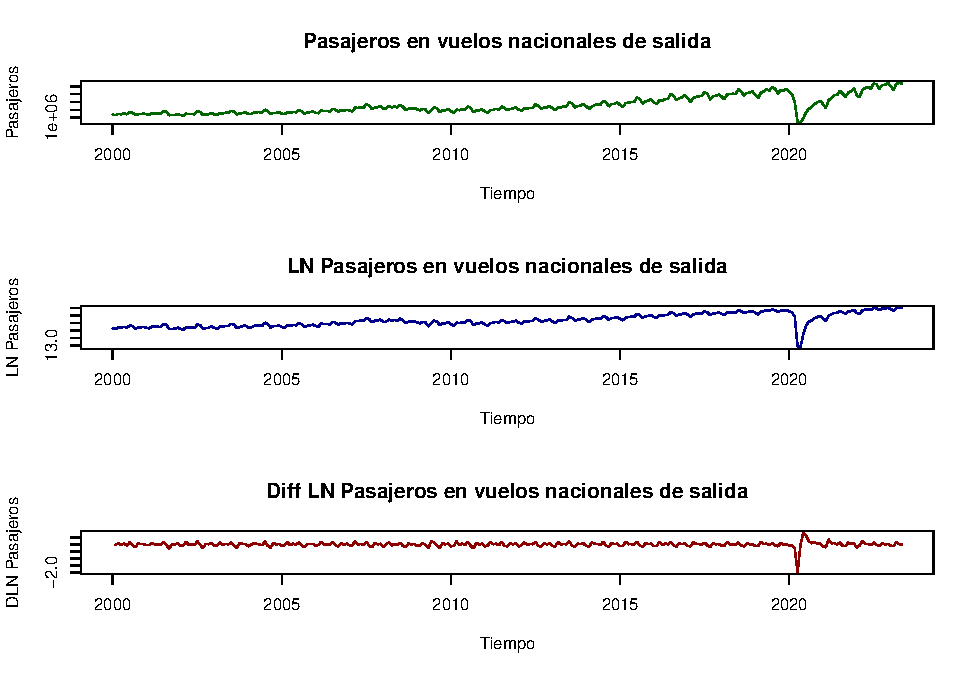
\includegraphics{Notas-Series-Tiempo_files/figure-latex/fig47-1} 

}

\caption{Pasajeros en vuelos de salidas nacionales en niveles y en diferencias logaritmicas}\label{fig:fig47}
\end{figure}

\begin{Shaded}
\begin{Highlighting}[]
\FunctionTok{par}\NormalTok{(}\AttributeTok{mfrow=}\FunctionTok{c}\NormalTok{(}\DecValTok{1}\NormalTok{,}\DecValTok{1}\NormalTok{))}
\end{Highlighting}
\end{Shaded}

A continuación, estimaremos un \(AR(2)\) para la serie en niveles bajo una transformación logarítmica (\(LPaxNal_t\)) y en diferencias logaritmitcas (\(DLPax_Nal_t\)). Para el primer caso obtenemos el siguiente resultado:

\begin{longtable}[]{@{}cccccc@{}}
\caption{\label{tab:AR02} AR(2) para la variable \(LPaxNal_t\).}\tabularnewline
\toprule\noalign{}
\endfirsthead
\endhead
\bottomrule\noalign{}
\endlastfoot
\(LPaxNal_t\) & \(=\) & \(14.6267\) & \(+\) & \(0.7637\) & \(LPaxNal_{t-1}\) \\
& & \((0.1816)\) & & \((0.0637)\) & \\
& & \(0.2025\) & \(LPaxNal_{t-2}\) & & \\
& & \((0.0646)\) & & & \\
\(\hat{\sigma}^2\) & \(=\) & \(0.01138\) & \(AIC\) & \(=\) & \(-372.64\) \\
\end{longtable}

Para el segundo caso obtenemos el siguiente resultado:

\begin{longtable}[]{@{}cccccc@{}}
\caption{\label{tab:AR0201} AR(2) para la variable \(DLPaxNal_t\).}\tabularnewline
\toprule\noalign{}
\endfirsthead
\endhead
\bottomrule\noalign{}
\endlastfoot
\(DLPaxNal_t\) & \(=\) & \(0.0050\) & \(+\) & \(0.3205\) & \(DLPaxNal_{t-1}\) \\
& & \((0.0036)\) & & \((0.0592)\) & \\
& & \(0.4242\) & \(DLPaxNal_{t-2}\) & & \\
& & \((0.0591)\) & & & \\
\(\hat{\sigma}^2\) & \(=\) & \(0.009378\) & \(AIC\) & \(=\) & \(-418.3\) \\
\end{longtable}

Para ambos casos, entre paréntesis indicamos los errores estándar y reportamos el estadístico de Akaike, AIC. Finalmente, podemos determinar si las soluciones serán convergentes para ello en la Figura \ref{fig:fig48} mostramos las raíces asociadas a cada uno de los polinomios. De la inspección visual, podemos concluir que ambas propuestas de AR(2) representan una solución convergente y estable.

\begin{Shaded}
\begin{Highlighting}[]
\FunctionTok{source}\NormalTok{(}\StringTok{"arroots.R"}\NormalTok{)}

\FunctionTok{source}\NormalTok{(}\StringTok{"plot.armaroots.R"}\NormalTok{)}

\NormalTok{AR\_LPax\_Nal }\OtherTok{\textless{}{-}} \FunctionTok{arima}\NormalTok{(LPax\_Nal, }\AttributeTok{order =} \FunctionTok{c}\NormalTok{(}\DecValTok{2}\NormalTok{, }\DecValTok{0}\NormalTok{, }\DecValTok{0}\NormalTok{), }
                     \AttributeTok{method =} \StringTok{"ML"}\NormalTok{)}

\NormalTok{AR\_DLPax\_Nal }\OtherTok{\textless{}{-}} \FunctionTok{arima}\NormalTok{(DLPax\_Nal, }\AttributeTok{order =} \FunctionTok{c}\NormalTok{(}\DecValTok{2}\NormalTok{, }\DecValTok{0}\NormalTok{, }\DecValTok{0}\NormalTok{), }
                      \AttributeTok{method =} \StringTok{"ML"}\NormalTok{)}

\FunctionTok{par}\NormalTok{(}\AttributeTok{mfrow=}\FunctionTok{c}\NormalTok{(}\DecValTok{1}\NormalTok{,}\DecValTok{2}\NormalTok{))}

\FunctionTok{plot.armaroots}\NormalTok{(}\FunctionTok{arroots}\NormalTok{(AR\_LPax\_Nal), }
               \AttributeTok{main=}\StringTok{"Inverse AR roots of }\SpecialCharTok{\textbackslash{}n}\StringTok{AR(2): LN Pax Nal"}\NormalTok{)}

\CommentTok{\#}
\FunctionTok{plot.armaroots}\NormalTok{(}\FunctionTok{arroots}\NormalTok{(AR\_DLPax\_Nal), }
               \AttributeTok{main=}\StringTok{"Inverse AR roots of }\SpecialCharTok{\textbackslash{}n}\StringTok{AR(2): Diff LN Pax Nal"}\NormalTok{)}
\end{Highlighting}
\end{Shaded}

\begin{figure}

{\centering 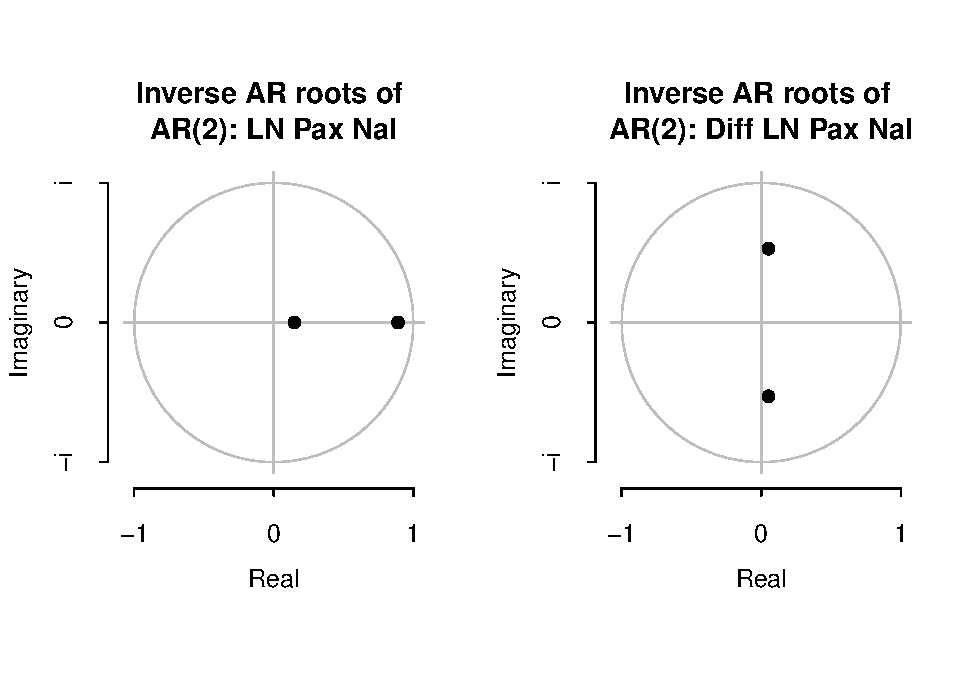
\includegraphics{Notas-Series-Tiempo_files/figure-latex/fig48-1} 

}

\caption{Inveso de las Raíces del polinomio característico}\label{fig:fig48}
\end{figure}

\begin{Shaded}
\begin{Highlighting}[]
\FunctionTok{par}\NormalTok{(}\AttributeTok{mfrow=}\FunctionTok{c}\NormalTok{(}\DecValTok{1}\NormalTok{,}\DecValTok{1}\NormalTok{))}
\end{Highlighting}
\end{Shaded}

\hypertarget{arp}{%
\subsection{AR(p)}\label{arp}}

Veremos ahora una generalización de los procesos autoregresivos (AR). Esta generalización es conocida como un proceso \(AR(p)\) y que puede ser descrito por la siguiente ecuación en diferencia estocástica:
\begin{equation}
    X_t = a_0 + a_1 X_{t-1} + a_2 X_{t-2} + a_3 X_{t-3} + \ldots + a_p X_{t-p} + U_t
    \label{eq:ARpEq}
\end{equation}

Donde \(a_p \neq 0\), y \(U_t\) es un proceso puramente aleatorio con media cero (0), varianza constante (\(\sigma^2\)) y covarianza cero (0). Usando el operador rezago, \(L^k\), para \(k = 0, 1, 2, \ldots, p\), obtenemos la siguiente expresión de la ecuación \eqref{eq:ARpEq}:
\begin{equation}
    (1 - a_1 L - a_2 L^2 - a_3 L^3 - \ldots - a_p L^p) X_t = a_0 + U_t
\end{equation}

Definamos el polinomio \(\alpha(L)\) como:
\begin{equation}
    \alpha(L) = 1 - a_1 L - a_2 L^2 - a_3 L^3 - \ldots - a_p L^p
    \label{eq:PolA}
\end{equation}

De forma similar que en los procesos \(AR(1)\) y \(AR(2)\), las condiciones de estabilidad del proceso \(AR(p)\) estarán dadas por la solución de la ecuación característica:
\begin{equation}
    \lambda^p - a_1 \lambda^{p-1} - a_2 \lambda^{p-2} - a_3 \lambda^{p-3} - \ldots - a_p = 0
\end{equation}

Así, solo si el polinomio anterior tiene raíces cuyo valor absoluto sea menor a uno (\$ \textbar{} \lambda\_i \textbar{} \textless{} 1 \$) y si \(1 - a_1 L - a_2 L^2 - a_3 L^3 - \ldots - a_p L^p < 1\) podremos decir que el proceso es convergente y estable. Lo anterior significa que la ecuación \eqref{eq:PolA} puede expresarse en términos de la descomposición de Wold o como la suma infinita de términos como:
\begin{equation}
    \frac{1}{1 - a_1 L  - a_2 L^2 - a_3 L^3  - \ldots - a_p L^p} = \psi_0 + \psi_1 L + \psi_2 L^2 + \psi_3 L^3 + \ldots
\end{equation}

Donde, por construcción de \(\alpha(L) \alpha^{-1}(L) = 1\) implica que \(\psi_0 = 1\). De forma similar a los procesos AR(1) y AR(2), es posible determinar el valor de los coeficientes \(\psi_j\) en términos de los coeficientes \(a_i\). Así, la solución del proceso \(AR(p)\) estará dada por:
\begin{equation}
    X_t = \frac{a_0}{1 - a_1  - a_2 - a_3  - \ldots - a_p} + \sum^{\infty}_{j = 0} \psi_j U_{t-j}
    \label{eq:ARpEqSol}
\end{equation}

Considerando la solución de la ecuación \eqref{eq:ARpEq} expresada en la ecuación \eqref{eq:ARpEqSol} podemos determinar los momentos del proceso y que estarán dados por una media como:
\begin{equation}
    \mathbb{E}[X_t] = \mu = \frac{a_o}{1 - a_1  - a_2 - a_3  - \ldots - a_p}
\end{equation}

Lo anterior, considerado que \(\mathbb{E}[U_t] = 0\), para todo \(t\). Para determinar la varianza del proceso, sin pérdida de generalidad, podemos definir una ecuación: \(\gamma(\tau) = \mathbb{E}[X_{t - \tau} X_t]\), la cual (omitiendo la constante, ya que la correlación de una constante con cuaquier variable aleatoria que depende del tiempo es cero (0)) puede ser escrita como:
\begin{equation}
    \gamma(\tau) = \mathbb{E}[(X_{t - \tau}) \cdot (a_1 X_{t-1} + a_2 X_{t-2} + a_3 X_{t-3} + \ldots + + a_p X_{t-p} + U_t)]
\end{equation}

Donde \(\tau = 0, 1, 2, \ldots, p\) y \(a_0 = 0\), lo que implica que \(\mu = 0\). De lo anterior obtenemos el siguiente conjunto de ecuaciones mediante sustituciones de los valores de \(\tau\):
\begin{eqnarray}
    \gamma(0) & = & a_1 \gamma(1) + a_2 \gamma(2) + \ldots + a_p \gamma(p) + \sigma^2 \nonumber \\
    \gamma(1) & = & a_1 \gamma(0) + a_2 \gamma(1) + \ldots + a_p \gamma(p-1) \nonumber \\
    \vdots \nonumber \\
    \gamma(p) & = & a_1 \gamma(p-1) + a_2 \gamma(p-2) + \ldots + a_p \gamma(0) \nonumber
\end{eqnarray}

De esta forma, es fácil observar que la ecuación general para \(p > 0\) estará dada por:
\begin{equation}
    \gamma(p) - a_1 \gamma(\tau - 1) - a_2 \gamma(\tau - 2) - \ldots - a_p \gamma(\tau - p) = 0
    \label{eq:Gammap}
\end{equation}

Dividiendo la ecuación \eqref{eq:Gammap} por \(\gamma(0)\), se obtiene la siguiente ecuación:
\begin{equation}
    \rho(p) - a_1 \rho(\tau - 1) + a_2 \rho(\tau - 2) + \ldots + a_p \rho(\tau - p) = 0
\end{equation}

Así, podemos escribir el siguiente sistema de ecuaciones:
\begin{eqnarray}
    \rho(1) & = & a_1 + a_2 \rho(1) + a_3 \rho(2) + \ldots + a_p \rho(p-1) \nonumber \\
    \rho(2) & = & a_1 \rho(1) + a_2 + a_3 \rho(1) + \ldots + a_p \rho(p-2) \nonumber \\
    & \vdots & \nonumber \\
    \rho(p) & = & a_1 \rho(p-1) + a_2 \rho(p-2) + \ldots + a_p \nonumber
\end{eqnarray}

Lo anterior se puede expresar como un conjunto de vectores y matrices de la siguiente forma:
\begin{equation}
    \left[ 
    \begin{array}{c}
        \rho(1) \\
        \rho(2) \\
        \vdots \\
        \rho(p)
    \end{array} 
    \right]
    = 
    \left[ 
    \begin{array}{c c c c}
        1 & \rho(1) & \ldots & \rho(p - 1) \\
        \rho(1) & 1 & \ldots & \rho(p - 2) \\
        \rho(2) & \rho(1) & \ldots & \rho(p - 3) \\
        \vdots & \vdots & \ldots & \vdots \\
        \rho(p - 1) & \rho(p - 2) & \ldots & 1 \\
    \end{array} 
    \right]
    \left[ 
    \begin{array}{c}
        a_1 \\
        a_2 \\
        a_3 \\
        \vdots \\
        a_p \\
    \end{array} 
    \right]
\end{equation}

De lo anterior podemos escribir la siguiente ecuación que es una forma alternativa para expresar los valores de los coeficientes \(a_i\) de la solución del proceso \(AR(p)\):
\begin{equation}
    \boldsymbol{\rho} = \mathbf{R} \mathbf{a}
\end{equation}

Es decir, podemos obtener la siguiente expresión:
\begin{equation}
    \mathbf{a} = \mathbf{R}^{-1} \boldsymbol{\rho}
\end{equation}

\textbf{Ejemplo}. Utilizaremos la serie de Pasajeros en vuelos internacionales de salida para estimar un \(AR(p)\) mediante el método de máxima verosimilitud (ML). Antes de realizar el proceso de estimación, consideremos una transformación de la serie en logaritmos y una más en diferencias logarítmicas; lo anterior con el objeto de obtener una serie de tiempo suavizada y expresada en tasas de crecimiento, con un comportamiento parecido a un proceso estacionario.

Primero, para decidir si se realizará un \(AR(p)\) para la serie en niveles o en diferencias, analizaremos su gráfica. La serie de Pasajeros en vuelos internacionales de salidas se muestra en la Figura \ref{fig:fig49}. En esta se muestra la gráfica de la serie en niveles (sin transformación logarítmica y con transformación logarítmica) y en diferencias logarítmicas mensuales (es decir, con diferencia respecto del mes inmediato anterior).

\begin{Shaded}
\begin{Highlighting}[]
\FunctionTok{library}\NormalTok{(ggplot2)}
\FunctionTok{library}\NormalTok{(dplyr)}
\FunctionTok{library}\NormalTok{(readxl)}
\FunctionTok{library}\NormalTok{(stats)}

\NormalTok{Datos }\OtherTok{\textless{}{-}} \FunctionTok{read\_excel}\NormalTok{(}\StringTok{"BD/Base\_Transporte.xlsx"}\NormalTok{, }
                    \AttributeTok{sheet =} \StringTok{"Datos"}\NormalTok{, }\AttributeTok{col\_names =} \ConstantTok{TRUE}\NormalTok{)}

\CommentTok{\# En Niveles}
\NormalTok{Pax\_Int }\OtherTok{\textless{}{-}} \FunctionTok{ts}\NormalTok{(Datos}\SpecialCharTok{$}\NormalTok{Pax\_Int, }
              \AttributeTok{start =} \FunctionTok{c}\NormalTok{(}\DecValTok{2000}\NormalTok{, }\DecValTok{1}\NormalTok{), }
              \AttributeTok{freq =} \DecValTok{12}\NormalTok{)}

\CommentTok{\# Logaritmos:}
\NormalTok{LPax\_Int }\OtherTok{\textless{}{-}} \FunctionTok{ts}\NormalTok{(}\FunctionTok{log}\NormalTok{(Datos}\SpecialCharTok{$}\NormalTok{Pax\_Int), }
               \AttributeTok{start =} \FunctionTok{c}\NormalTok{(}\DecValTok{2000}\NormalTok{, }\DecValTok{1}\NormalTok{), }
               \AttributeTok{freq =} \DecValTok{12}\NormalTok{)}

\CommentTok{\# Diferencias mensuales:}
\NormalTok{DLPax\_Int }\OtherTok{\textless{}{-}} \FunctionTok{ts}\NormalTok{(}\FunctionTok{log}\NormalTok{(Datos}\SpecialCharTok{$}\NormalTok{Pax\_Int) }\SpecialCharTok{{-}} \FunctionTok{lag}\NormalTok{(}\FunctionTok{log}\NormalTok{(Datos}\SpecialCharTok{$}\NormalTok{Pax\_Int), }\DecValTok{1}\NormalTok{),}
                \AttributeTok{start =} \FunctionTok{c}\NormalTok{(}\DecValTok{2000}\NormalTok{, }\DecValTok{1}\NormalTok{), }
                \AttributeTok{freq =} \DecValTok{12}\NormalTok{)}

\CommentTok{\#}
\FunctionTok{par}\NormalTok{(}\AttributeTok{mfrow=}\FunctionTok{c}\NormalTok{(}\DecValTok{3}\NormalTok{,}\DecValTok{1}\NormalTok{))}

\FunctionTok{plot}\NormalTok{(Pax\_Int, }\AttributeTok{xlab =} \StringTok{"Tiempo"}\NormalTok{, }\AttributeTok{ylab =} \StringTok{"Pasajeros"}\NormalTok{,}
     \AttributeTok{main =} \StringTok{"Pasajeros en vuelos internacionales de salida"}\NormalTok{,}
     \AttributeTok{col =} \StringTok{"darkgreen"}\NormalTok{)}

\FunctionTok{plot}\NormalTok{(LPax\_Int, }\AttributeTok{xlab =} \StringTok{"Tiempo"}\NormalTok{, }\AttributeTok{ylab =} \StringTok{"LN Pasajeros"}\NormalTok{,}
     \AttributeTok{main =} \StringTok{"LN Pasajeros en vuelos internacionales de salida"}\NormalTok{,}
     \AttributeTok{col =} \StringTok{"darkblue"}\NormalTok{)}

\FunctionTok{plot}\NormalTok{(DLPax\_Int, }\AttributeTok{xlab =} \StringTok{"Tiempo"}\NormalTok{, }\AttributeTok{ylab =} \StringTok{"DLN Pasajeros"}\NormalTok{,}
     \AttributeTok{main =} \StringTok{"Diff LN Pasajeros en vuelos internacionales de salia"}\NormalTok{, }
     \AttributeTok{col =} \StringTok{"darkred"}\NormalTok{)}
\end{Highlighting}
\end{Shaded}

\begin{figure}

{\centering 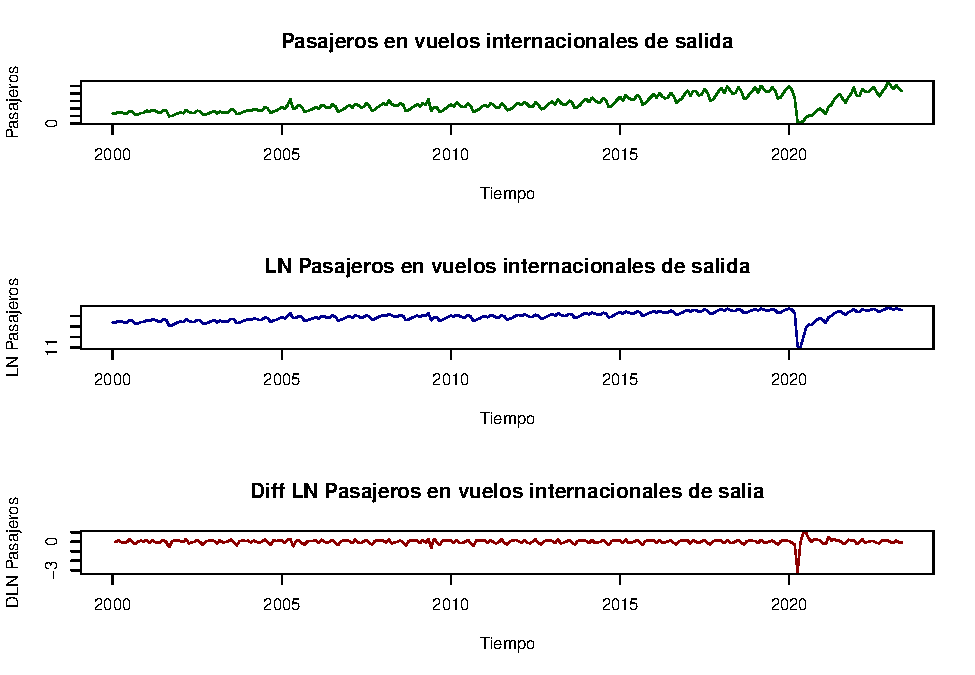
\includegraphics{Notas-Series-Tiempo_files/figure-latex/fig49-1} 

}

\caption{Pasajeros en vuelos internacionales de salida en niveles y en diferencias logaritmicas}\label{fig:fig49}
\end{figure}

\begin{Shaded}
\begin{Highlighting}[]
\FunctionTok{par}\NormalTok{(}\AttributeTok{mfrow=}\FunctionTok{c}\NormalTok{(}\DecValTok{1}\NormalTok{,}\DecValTok{1}\NormalTok{))}
\end{Highlighting}
\end{Shaded}

De la gráfica en la Figura \ref{fig:fig49} observamos que quizá la mejor forma de estimar un \(AR(p)\) es mediante la serie en diferencias, ya que ésta es la que parece ser una serie estacionaria. A continuación, estimaremos una AR(4) para la serie en diferencias logarítmicas (\(DLPaxInt_t\)):

\begin{longtable}[]{@{}cccccc@{}}
\caption{\label{tab:AR04} AR(4) para la variable \(DLPaxInt_t\).}\tabularnewline
\toprule\noalign{}
\endfirsthead
\endhead
\bottomrule\noalign{}
\endlastfoot
\(DLPaxInt_t\) & \(=\) & \(0.0050\) & \(+\) & \(0.2701\) & \(DLPaxInt_{t-1}\) \\
& & \((0.0052)\) & & \((0.0655)\) & \\
& & \(-0.4326\) & \(DLPaxNal_{t-2}\) & & \\
& & \((0.0664)\) & & & \\
& & \(-0.1956\) & \(DLPaxNal_{t-3}\) & & \\
& & \((0.0664)\) & & & \\
& & \(-0.0316\) & \(DLPaxNal_{t-4}\) & & \\
& & \((0.0653)\) & & & \\
\(\hat{\sigma}^2\) & \(=\) & \(0.02371\) & \(AIC\) & \(=\) & \(-198.16\) \\
\end{longtable}

Entre paréntesis indicamos los errores estándar y reportamos el estadístico de Akaike, AIC. Finalmente, podemos determinar si las soluciones serán convergentes, para ello en la Figura \ref{fig:fig410} mostramos las raíces asociadas a cada uno de los polinomios. De la inspección visual podemos concluir que el AR(4) representan una solución convergente y estable.

\begin{Shaded}
\begin{Highlighting}[]
\FunctionTok{source}\NormalTok{(}\StringTok{"arroots.R"}\NormalTok{)}

\FunctionTok{source}\NormalTok{(}\StringTok{"plot.armaroots.R"}\NormalTok{)}

\NormalTok{AR\_LPax\_Int }\OtherTok{\textless{}{-}} \FunctionTok{arima}\NormalTok{(LPax\_Int, }\AttributeTok{order =} \FunctionTok{c}\NormalTok{(}\DecValTok{4}\NormalTok{, }\DecValTok{0}\NormalTok{, }\DecValTok{0}\NormalTok{), }
                     \AttributeTok{method =} \StringTok{"ML"}\NormalTok{)}

\NormalTok{AR\_DLPax\_Int }\OtherTok{\textless{}{-}} \FunctionTok{arima}\NormalTok{(DLPax\_Int, }\AttributeTok{order =} \FunctionTok{c}\NormalTok{(}\DecValTok{4}\NormalTok{, }\DecValTok{0}\NormalTok{, }\DecValTok{0}\NormalTok{), }
                      \AttributeTok{method =} \StringTok{"ML"}\NormalTok{)}

\FunctionTok{par}\NormalTok{(}\AttributeTok{mfrow=}\FunctionTok{c}\NormalTok{(}\DecValTok{1}\NormalTok{,}\DecValTok{2}\NormalTok{))}

\FunctionTok{plot.armaroots}\NormalTok{(}\FunctionTok{arroots}\NormalTok{(AR\_LPax\_Nal), }
               \AttributeTok{main=}\StringTok{"Inverse AR roots of }\SpecialCharTok{\textbackslash{}n}\StringTok{AR(2): LN Pax Int"}\NormalTok{)}

\CommentTok{\#}
\FunctionTok{plot.armaroots}\NormalTok{(}\FunctionTok{arroots}\NormalTok{(AR\_DLPax\_Nal), }
               \AttributeTok{main=}\StringTok{"Inverse AR roots of }\SpecialCharTok{\textbackslash{}n}\StringTok{AR(2): Diff LN Pax Int"}\NormalTok{)}
\end{Highlighting}
\end{Shaded}

\begin{figure}

{\centering 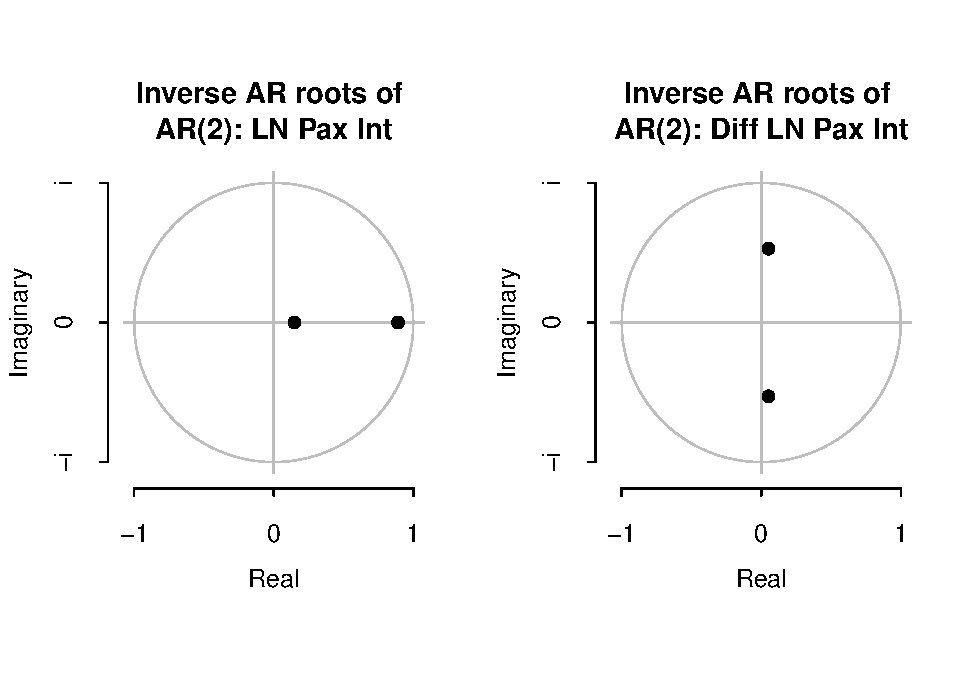
\includegraphics{Notas-Series-Tiempo_files/figure-latex/fig410-1} 

}

\caption{Inveso de las Raíces del polinomio característico}\label{fig:fig410}
\end{figure}

\begin{Shaded}
\begin{Highlighting}[]
\FunctionTok{par}\NormalTok{(}\AttributeTok{mfrow=}\FunctionTok{c}\NormalTok{(}\DecValTok{1}\NormalTok{,}\DecValTok{1}\NormalTok{))}
\end{Highlighting}
\end{Shaded}

\hypertarget{procesos-de-medias-muxf3viles-ma}{%
\section{Procesos de Medias Móviles (MA)}\label{procesos-de-medias-muxf3viles-ma}}

\hypertarget{ma1}{%
\subsection{MA(1)}\label{ma1}}

Una vez planteado el proceso generalizado de \(AR(p)\), iniciamos el planteamiento de los procesos de medias móviles, denotados como \(MA(q)\). Iniciemos con el planteamiento del proceso \(MA(1)\), que se puede escribir como una ecuación como la siguiente:
\begin{equation}
    X_t = \mu + U_t - b_1 U_{t-1}
    \label{eq:MA1Eq}
\end{equation}

O como:
\begin{equation}
    X_t - \mu = (1 - b_1 L) U_{t}
\end{equation}

Donde \(U_t\) es un proceso puramente aleatorio, es decir, con \(\mathbb{E}[U_t] = 0\), \(Var[U_t] = \sigma^2\), y \(Cov[U_t, U_s] = 0\). Así, un proceso \(MA(1)\) puede verse como un proceso AR con una descomposición de Wold en la que \(\psi_0 = 1\), \(\psi_1 = - b_1\) y \(\psi_j = 0\) para todo \(j > 1\).

Al igual que los procesos autoregresivos, determinaremos los momentos de un proceso \(MA(1)\). En el caso de la media, observamos que será:
\begin{eqnarray}
    \mathbb{E}[X_t] & = & \mu + \mathbb{E}[U_t] - b_1 \mathbb{E}[U_{t - 1}] \nonumber \\
    & = & \mu
\end{eqnarray}

Por su parte, la varianza estará dada por:
\begin{eqnarray}
    Var[X_t] & = & \mathbb{E}[(X_t - \mu)^2] \nonumber \\
    & = & \mathbb{E}[(U_t - b_1 U_{t-1})^2] \nonumber \\
    & = & \mathbb{E}[U_t^2 - 2 b_1 U_t U_{t-1} + b_1^2 U_{t - 1}^2] \nonumber \\
    & = &\mathbb{E}[U_t^2] - 2 b_1 \mathbb{E}[U_t U_{t-1}] + b_1^2 \mathbb{E}[U_{t - 1}^2]] \nonumber \\
    & = & \sigma^2 + b_1^2 \sigma^2 \nonumber \\
    & = & (1 + b_1^2) \sigma^2 = \gamma(0)
\end{eqnarray}

De esta forma, la varianza del proceso es constante en cualquier periodo \(t\). Para determinar la covarianza utilizaremos la siguiente ecuación:
\begin{eqnarray}
    \mathbb{E}[(x_t - \mu)(x_{t + \tau} - \mu)] & = & \mathbb{E}[(U_t - b_1 U_{t-1})(U_{t + \tau} - b_1 U_{t + \tau - 1})] \nonumber \\
    & = & \mathbb{E}[U_t U_{t + \tau} - b_1 U_t U_{t + \tau - 1} - b_1 U_{t - 1} U_{t + \tau} \nonumber \\
    &   & + b_1^2 U_{t - 1} U_{t + \tau - 1}] \nonumber \\
    & = & \mathbb{E}[U_t U_{t + \tau}] - b_1 \mathbb{E}[U_t U_{t + \tau - 1}] \nonumber \\
    &   & - b_1 \mathbb{E}[U_{t - 1} U_{t + \tau}] + b_1^2 \mathbb{E}[U_{t - 1} U_{t + \tau - 1}]
    \label{eq:MA1Cov}
\end{eqnarray}

Si hacemos sustituciones de diferentes valores de \(\tau\) en la ecuación \eqref{eq:MA1Cov} notaremos que la covarianza será distinta de cero únicamente para el caso de \(\tau = 1, -1\). En ambos casos tendremos como resultado:
\begin{eqnarray}
    \mathbb{E}[(x_t - \mu)(x_{t + 1} - \mu)] & = & \mathbb{E}[(x_t - \mu)(x_{t - 1} - \mu)] \nonumber \\
    & = & - b_1 \mathbb{E}[U_t U_{t}] \nonumber \\
    & = & - b_1 \mathbb{E}[U_{t - 1} U_{t - 1}] \nonumber \\ 
    & = & - b_1^2 \sigma^2 = \gamma(1)
\end{eqnarray}

De esta forma tendremos que las funciones de autocorrelación estarán dadas por los siguientes casos:
\begin{eqnarray}
    \rho(0) & = & 1 \nonumber \\
    \rho(1) & = & \frac{- b_1}{1 + b_1^2} \nonumber \\
    \rho(\tau) & = & 0 \text{ para todo } \tau > 1 \nonumber 
\end{eqnarray}

Ahora regresando a la ecuación \eqref{eq:MA1Eq}, su solución la podemos expresar como:
\begin{eqnarray}
    U_ t & = & - \frac{\mu}{1 - b_1} + \frac{1}{1 - b_1 L} X_t \nonumber \\
    & = & - \frac{\mu}{1 - b_1} + X_t + b_1 X_{t-1} + b_1^2 X_{t-2} + \ldots \nonumber
\end{eqnarray}

Donde la condición para que se cumpla esta ecuación es que \$ \textbar{} b\_1 \textbar{} \textless{} 1 \$. La manera de interpretar esta condición es como una condición de estabilidad de la solución y cómo una condición de invertibilidad. Notemos que un \(MA(1)\) (y en general un \(MA(q)\)) es equivalente a un \(AR(\infty)\), es decir, cuando se invierte un MA se genera un AR con infinitos rezagos.

En esta sección no desarrollaremos un ejemplo, primero explicaremos en qué consiste una modelación del tipo \(MA(q)\) y después plantearemos un ejemplo en concreto.

\hypertarget{maq}{%
\subsection{MA(q)}\label{maq}}

En general, el proceso de medias móviles de orden \(q\), \(MA(q)\), puede ser escrito como:
\begin{equation}
    X_t = \mu + U_t - b_1 U_{t-1} - b_2 U_{t-2} - \ldots - b_q U_{t-q}
    \label{eq:MAqEQ}
\end{equation}

Podemos reescribir la ecuación \eqref{eq:MAqEQ} utilizando el operador rezago. Así, tendremos el proceso de \(MA(q)\) como:
\begin{eqnarray}
    X_t - \mu & = & (1 - b_1 L - b_2 L^2 - \ldots - b_q L^q) U_{t} \nonumber \\
    X_t - \mu & = & \beta(L) U_t
    \label{eq:MAqRed}
\end{eqnarray}

Donde \(U_t\) es un proceso puramente aleatorio con \(\mathbb{E}[U_t] = 0\), \(Var[U_t] = \mathbb{E}[U_t^2] = 0\) y \(Cov[U_t, U_s] = \mathbb{E}[U_t, U_s] = 0\), y \(\beta(L) = 1 - b_1 L - b_2 L^2 - \ldots - b_q L^q\) es un polinomio del operador rezago \(L\). La ecuación \eqref{eq:MAqRed} puede ser interpretada como un proceso \(AR(q)\) sobre la serie \(U_t\).

Ahora determinemos los momentos de un proceso \(MA(q)\):
\begin{eqnarray}
    \mathbb{E}[X_t] & = & \mathbb{E}[\mu + U_t - b_1 U_{t-1} - b_2 U_{t-2} - \ldots - b_q U_{t-q}] \nonumber \\
    & = & \mu + \mathbb{E}[U_t] - b_1 \mathbb{E}[U_{t-1}] - b_2 \mathbb{E}[U_{t-2}] - \ldots - b_q \mathbb{E}[U_{t-q}] \nonumber \\
    & = & \mu
\end{eqnarray}

En el caso de la varianza tenemos que se puede expresar como:
\begin{eqnarray}
    Var[X_t] & = & \mathbb{E}[(X_t - \mu)^2] \nonumber \\
    & = & \mathbb{E}[(U_t - b_1 U_{t-1} - b_2 U_{t-2} - \ldots - b_q U_{t-q})^2] \nonumber \\
    & = & \mathbb{E}[U_t^2 + b_1^2 U_{t-1}^2 + b_2^2 U_{t-2}^2 + \ldots + b_q^2 U_{t-q}^2 \nonumber \\
    &   & - 2 b_1 U_t U_{t - 1} - \ldots - 2 b_{q - 1} b_q U_{t - q + 1} U_{t - q}] \nonumber \\
    & = & \mathbb{E}[U_t^2] + b_1^2 \mathbb{E}[U_{t-1}^2] + b_2^2 \mathbb{E}[U_{t-2}^2] + \ldots + b_q^2 \mathbb{E}[U_{t-q}^2] \nonumber \\
    &   & - 2 b_1 \mathbb{E}[U_t U_{t - 1}] - \ldots - 2 b_{q - 1} b_q \mathbb{E}[U_{t - q + 1} U_{t - q}] \nonumber \\
    & = & \sigma^2 + b^2_1 \sigma^2 + b^2_2 \sigma^2 + \ldots + b^2_q \sigma^2 \nonumber \\
    & = & (1 + b^2_1 + b^2_2 + \ldots + b^2_q) \sigma^2
\end{eqnarray}

En el caso de las covarianzas podemos utilizar una idea similar al caso del \(AR(p)\), construir una expresión general para cualquier rezago \(\tau\):
\begin{eqnarray}
    Cov[X_t, X_{t + \tau}] & = & \mathbb{E}[(X_t - \mu)(X_{t + \tau} - \mu)] \nonumber \\
    & = & \mathbb{E}[(U_t - b_1 U_{t-1} - b_2 U_{t-2} - \ldots - b_q U_{t-q}) \nonumber \\
    &   & (U_{t + \tau} - b_1 U_{t + \tau -1} - b_2 U_{t + \tau -2} - \ldots - b_q U_{t + \tau - q})] \nonumber
\end{eqnarray}

La expresión anterior se puede desarrollar para múltiples casos de \(\tau = 1, 2, \ldots, q\). De esta forma tenemos el siguiente sistema:
\begin{eqnarray}
    \tau = 1 & : & \gamma(1) = (- b_1 + b_1 b_2 + \ldots + b_{q-1} b_q) \sigma^2 \nonumber \\
    \tau = 2 & : & \gamma(2) = (- b_2 + b_1 b_3 + \ldots + b_{q-2} b_q) \sigma^2 \nonumber \\
    & \vdots & \nonumber \\
    \tau = q & : & \gamma(q) = b_q \sigma^2 \nonumber
\end{eqnarray}

Donde \(\gamma(\tau) = 0\) para todo \(\tau > q\). Es decir, todas las autocovarianzas y autocorrelaciones con órdenes superiores a \(q\) son cero (0). De esta forma, esta característica teórica permite identificar el orden de \(MA(q)\) visualizando la función de autocorrelación y verificando a partir de cuál valor de rezago la autocorrelación es no significativa.

Regresando al problema original que es el de determinar una solución para la ecuación \eqref{eq:MAqEQ}, tenemos que dicha solución estará dada por un \(AR(\infty)\) en términos de \(U_t\):
\begin{eqnarray}
    U_t & = & - \frac{\mu}{1 - b_1 - b_2 - \ldots - b_q} + \beta(L)^{-1} X_t \nonumber \\
    &   & - \frac{\mu}{1 - b_1 - b_2 - \ldots - b_q} + \sum_{j = 0}^{\infty} c_j X_{t-j} 
    \label{eq:MAqEQSol}
\end{eqnarray}

Donde se cumple que: \(1 = (1 - b_1 L^1 - b_2 L^2 - \ldots - b_q L^q)(1 - c_1 L - c_2 L^2 - \ldots)\) y los coeficientes \(c_j\) se pueden determinar por un método de coeficientes indeterminados y en términos de los valores \(b_i\). De igual forma que en el caso de la ecuación \eqref{eq:ARpEq}, en la ecuación \eqref{eq:MAqEQSol} se deben cumplir condiciones de estabilidad asociadas con las raíces del polinomio característico dado por:
\begin{equation}
    1 - b_1 x - b_2 x^2 - \ldots b_q x^q = 0
\end{equation}

El cual debe cumplir que \$ \textbar{} x\_i \textbar{} \textless{} 1 \$ y que \(1 - b_1 - b_2 - \ldots b_q < 1\).

\textbf{Ejemplo}. Ahora veamos un ejemplo del proceso \(MA(q)\), para lo cual retomaremos la serie de Pasajeros transportados en el metro de la CDMX (\(PaxMetro\)). Estimaremos el \(MA(q)\) mediante el método de máxima verosimilitud (ML). Antes de realizar el proceso de estimación, consideremos una transformación de la serie en logaritmos y una más en diferencias logarítmicas; lo anterior con el objeto de obtener una serie de tiempo suavizada y expresada en tasas de crecimiento, con un comportamiento parecido a un proceso estacionario.

La serie de Pasajeros transportados en el metro de la CDMX se muestra en la Figura \ref{fig:fig46}. En esta, se muestra la gráfica de la serie en niveles (sin transformación logarítmica y con transformación logarítmica) y en diferencias logarítmicas mensuales (es decir, con una diferencia respecto del mes inmediato anterior). Utilizaremos la serie en diferencias, ya que es la que parece ser estacionaria. Esta serie tiene la peculiaridad de que tiene un salto a la baja y uno al alza entre septiembre de 2017 y octubre de 2017. Para controlar ese efecto, en nuestro modelo \(MA(q)\) incluiremos dos variables dummies para dichos meses.

A continuación, estimaremos una \(MA(4)\) para la serie en diferencias:

\begin{longtable}[]{@{}cccccc@{}}
\caption{\label{tab:MA04} MA(4) para la variable \(DLPaxMetro_t\).}\tabularnewline
\toprule\noalign{}
\endfirsthead
\endhead
\bottomrule\noalign{}
\endlastfoot
\(DLPaxMetro_t\) & \(=\) & \(0.0000\) & \(-\) & \(0.7804\) & \(U_{t-1}\) \\
& & \((0.0000)\) & & \((0.0661)\) & \\
& \(+\) & \(0.3591\) & \(U_{t-2}\) & & \\
& & \((0.0826)\) & & & \\
& \(-\) & \(0.2775\) & \(U_{t-3}\) & & \\
& & \((0.0908)\) & & & \\
& \(-\) & \(0.1120\) & \(U_{t-4}\) & & \\
& & \((0.0769)\) & & & \\
& \(-\) & \(0.3789\) & \(DSep2017\) & & \\
& & \((0.0436)\) & & & \\
& \(+\) & \(0.3695\) & \(DOct2017\) & & \\
& & \((0.0434)\) & & & \\
\(\hat{\sigma}^2\) & \(=\) & \(0.002176\) & \(AIC\) & \(=\) & \(-749.94\) \\
\end{longtable}

Entre parentésis indicamos los errores estándar y al final reportamos el estadístico de Akaike, AIC. Finalmente, podemos determinar si la solución serán convergente, para ello en la Figura \ref{fig:fig411} mostramos las raíces asociadas a cada uno de los polinomios. De la inspección visual, podemos concluir que ambas propuestas de MA(4) representan una solución convergente y estable.

\begin{Shaded}
\begin{Highlighting}[]
\FunctionTok{library}\NormalTok{(ggplot2)}
\FunctionTok{library}\NormalTok{(dplyr)}
\FunctionTok{library}\NormalTok{(readxl)}
\FunctionTok{library}\NormalTok{(stats)}

\NormalTok{Datos }\OtherTok{\textless{}{-}} \FunctionTok{read\_excel}\NormalTok{(}\StringTok{"BD/Base\_Transporte\_ARIMA.xlsx"}\NormalTok{, }
                    \AttributeTok{sheet =} \StringTok{"Datos"}\NormalTok{, }\AttributeTok{col\_names =} \ConstantTok{TRUE}\NormalTok{)}

\FunctionTok{source}\NormalTok{(}\StringTok{"maroots.R"}\NormalTok{)}

\FunctionTok{source}\NormalTok{(}\StringTok{"plot.armaroots.R"}\NormalTok{)}

\NormalTok{Pax\_Metro }\OtherTok{\textless{}{-}} \FunctionTok{ts}\NormalTok{(Datos}\SpecialCharTok{$}\NormalTok{Pax\_Metro, }
                \AttributeTok{start =} \FunctionTok{c}\NormalTok{(}\DecValTok{2000}\NormalTok{, }\DecValTok{1}\NormalTok{), }
                \AttributeTok{freq =} \DecValTok{12}\NormalTok{)}

\NormalTok{LPax\_Metro }\OtherTok{\textless{}{-}} \FunctionTok{ts}\NormalTok{(}\FunctionTok{log}\NormalTok{(Datos}\SpecialCharTok{$}\NormalTok{Pax\_Metro), }
                 \AttributeTok{start =} \FunctionTok{c}\NormalTok{(}\DecValTok{2000}\NormalTok{, }\DecValTok{1}\NormalTok{), }
                 \AttributeTok{freq =} \DecValTok{12}\NormalTok{)}

\NormalTok{DLPax\_Metro }\OtherTok{\textless{}{-}} \FunctionTok{ts}\NormalTok{(}\FunctionTok{log}\NormalTok{(Datos}\SpecialCharTok{$}\NormalTok{Pax\_Metro) }\SpecialCharTok{{-}} 
                  \FunctionTok{lag}\NormalTok{(}\FunctionTok{log}\NormalTok{(Datos}\SpecialCharTok{$}\NormalTok{Pax\_Metro), }\DecValTok{1}\NormalTok{),}
                  \AttributeTok{start =} \FunctionTok{c}\NormalTok{(}\DecValTok{2000}\NormalTok{, }\DecValTok{1}\NormalTok{), }
                  \AttributeTok{freq =} \DecValTok{12}\NormalTok{)}

\NormalTok{D\_Sep2017 }\OtherTok{\textless{}{-}} \FunctionTok{ts}\NormalTok{(Datos}\SpecialCharTok{$}\NormalTok{D\_Sep2017, }
                \AttributeTok{start =} \FunctionTok{c}\NormalTok{(}\DecValTok{2000}\NormalTok{, }\DecValTok{1}\NormalTok{), }
                \AttributeTok{freq =} \DecValTok{12}\NormalTok{)}

\NormalTok{D\_Abr2020 }\OtherTok{\textless{}{-}} \FunctionTok{ts}\NormalTok{(Datos}\SpecialCharTok{$}\NormalTok{D\_Abr2020, }
                \AttributeTok{start =} \FunctionTok{c}\NormalTok{(}\DecValTok{2000}\NormalTok{, }\DecValTok{1}\NormalTok{), }
                \AttributeTok{freq =} \DecValTok{12}\NormalTok{)}

\NormalTok{D\_May2020   }\OtherTok{\textless{}{-}} \FunctionTok{ts}\NormalTok{(Datos}\SpecialCharTok{$}\NormalTok{D\_May2020, }
                \AttributeTok{start =} \FunctionTok{c}\NormalTok{(}\DecValTok{2000}\NormalTok{, }\DecValTok{1}\NormalTok{), }
                \AttributeTok{freq =} \DecValTok{12}\NormalTok{)}

\NormalTok{MA\_LPax\_Metro }\OtherTok{\textless{}{-}} \FunctionTok{arima}\NormalTok{(LPax\_Metro, }\AttributeTok{order =} \FunctionTok{c}\NormalTok{(}\DecValTok{0}\NormalTok{, }\DecValTok{0}\NormalTok{, }\DecValTok{4}\NormalTok{), }
                       \AttributeTok{method =} \StringTok{"ML"}\NormalTok{)}

\NormalTok{MA\_LPax\_Metro\_2 }\OtherTok{\textless{}{-}} \FunctionTok{arima}\NormalTok{(LPax\_Metro, }\AttributeTok{order =} \FunctionTok{c}\NormalTok{(}\DecValTok{0}\NormalTok{, }\DecValTok{0}\NormalTok{, }\DecValTok{4}\NormalTok{),}
                       \AttributeTok{xreg =} \FunctionTok{cbind}\NormalTok{(D\_Abr2020, D\_Sep2017, }
\NormalTok{                                    D\_May2020),}
                       \AttributeTok{method =} \StringTok{"ML"}\NormalTok{)}

\FunctionTok{par}\NormalTok{(}\AttributeTok{mfrow=}\FunctionTok{c}\NormalTok{(}\DecValTok{1}\NormalTok{,}\DecValTok{2}\NormalTok{))}

\FunctionTok{plot.armaroots}\NormalTok{(}\FunctionTok{maroots}\NormalTok{(MA\_LPax\_Metro), }
               \AttributeTok{main=}\StringTok{"Inverse MA roots of }\SpecialCharTok{\textbackslash{}n}\StringTok{MA(p): LN PAx Metro"}\NormalTok{)}

\FunctionTok{plot.armaroots}\NormalTok{(}\FunctionTok{maroots}\NormalTok{(MA\_LPax\_Metro\_2), }
               \AttributeTok{main=}\StringTok{"Inverse MA roots of }\SpecialCharTok{\textbackslash{}n}\StringTok{MA(p): LN PAx Metro con Dummy"}\NormalTok{)}
\end{Highlighting}
\end{Shaded}

\begin{figure}

{\centering 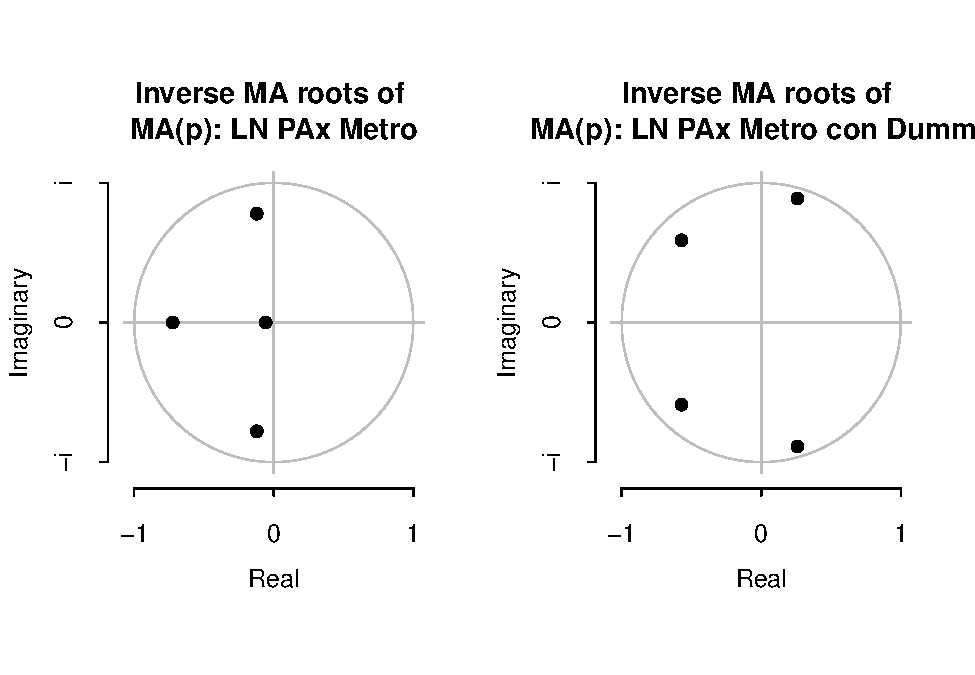
\includegraphics{Notas-Series-Tiempo_files/figure-latex/fig411-1} 

}

\caption{Inveso de las Raíces del polinomio característico}\label{fig:fig411}
\end{figure}

\begin{Shaded}
\begin{Highlighting}[]
\FunctionTok{par}\NormalTok{(}\AttributeTok{mfrow=}\FunctionTok{c}\NormalTok{(}\DecValTok{1}\NormalTok{,}\DecValTok{1}\NormalTok{))}
\end{Highlighting}
\end{Shaded}

\hypertarget{procesos-armap-q-y-arimap-d-q}{%
\section{Procesos ARMA(p, q) y ARIMA(p, d, q)}\label{procesos-armap-q-y-arimap-d-q}}

Hemos establecido algunas relaciones de los procesos AR y los procesos MA, es decir, cómo un \(MA(q)\) de la serie \(X_t\) puede ser reexpresada como un \(AR(\infty)\) de la serie \(U_t\), y viceversa un \(AR(p)\) de la serie \(X_t\) puede ser reeexpresada como un \(MA(\infty)\).

En este sentido, para cerrar esta sección veamos el caso de la especificación que conjunta ambos modelos en un modelo general conocido como \(ARMA(p, q)\) o \(ARIMA(p, d, q)\). La diferencia entre el primero y el segundo es las veces que se tuvo que diferenciar la serie analizada, registro que se lleva en el índice \(d\) de los parámetros dentro del concepto \(ARIMA(p, d, q)\). No obstante, en general nos referiremos al modelo como \(ARMA(p, q)\) y dependerá del analista si modela la serie en niveles (por ejemplo, en logaritmos) o en diferencias logarítmicas (o diferencias sin logaritmos).

\hypertarget{arma1-1}{%
\subsection{ARMA(1, 1)}\label{arma1-1}}

Dicho lo anterior, vamos a empezar con el análisis de un \(ARMA(1, 1)\). Un proceso \(ARMA(1, 1)\) puede verse como:
\begin{equation}
    X_t = \delta + a_1 X_{t - 1} + U_t - b_1 U_{t - 1}
    \label{eq:ARMA11Eq}
\end{equation}

Aplicando el operado rezago podemos rescribir la ecuación \eqref{eq:ARMA11Eq} como:
\begin{equation}
    (1 - a_1 L) X_t = \delta + (1 - b_1 L) U_t
\end{equation}

Donde \(U_t\) es un proceso puramente aleatorio como en los casos de \(AR(p)\) y \(MA(q)\), y \(X_t\) puede ser una serie en niveles o en diferencias (ambas, en términos logarítmicos).

Así, el modelo \(ARIMA (p, q)\) también tiene una representación de Wold que estará dada por las siguientes expresiones:
\begin{equation}
    X_t = \frac{\delta}{1 - a_1} + \frac{1 - b_1 L}{1 - a_1 L} U_t
    \label{eq:ARMA11Prev}
\end{equation}

Donde \(a_1 \neq b_1\), puesto que en caso contrario \(X_t\) sería un proceso puramente aleatorio con una media \(\mu = \frac{\delta}{1 - a_1}\). Así, podemos reescribir la descomposición de Wold a partir del componente de la ecuación \eqref{eq:ARMA11Prev}:
\begin{equation}
    \frac{1 - b_1 L}{1 - a_1 L} = \psi_0 + \psi_1 L + \psi_2 L^2 + \psi_3 L^3 + \ldots 
    \label{eq:ARMA11EqWold}
\end{equation}

Está ecuación es equivalente a la expresión:
\begin{eqnarray}
    (1 - b_1 L) & = & (1 - a_1 L)(\psi_0 + \psi_1 L + \psi_2 L^2 + \psi_3 L^3 + \ldots) \nonumber \\
    & = & \psi_0 + \psi_1 L + \psi_2 L^2 + \psi_3 L^3 + \ldots \nonumber \\
    &   & - a_1 \psi_0 L - a_1 \psi_1 L^2 - a_2 \psi_2 L^3 - a_1 \psi_3 L^4 - \ldots \nonumber
\end{eqnarray}

De esta forma podemos establecer el siguiente sistema de coeficientes indeterminados:
\begin{eqnarray*}
    L^0 & : & \Rightarrow \psi_0 = 1 \\
    L^1 & : & \psi_1 - a_1 \psi_0 = - b_1 \Rightarrow \psi_1 = a_1 - b_1 \\
    L^2 & : & \psi_2 - a_1 \psi_1 = 0 \Rightarrow \psi_2 = a_1(a_1 - b_1) \\
    L^3 & : & \psi_3 - a_1 \psi_2 = 0 \Rightarrow \psi_3 = a^2_1(a_1 - b_1) \\
     & \vdots &  \\
    L^j & : & \psi_j - a_1 \psi_{j - 1} = 0 \Rightarrow \psi_j = a^{j - 1}_1(a_1 - b_1)
\end{eqnarray*}

Así, la solución a la ecuación \eqref{eq:ARMA11Eq} estará dada por la siguiente generalización:
\begin{equation}
    X_t = \frac{\delta}{1 - a_1} + U_t + (a_1 - b_1) U_{t - 1} + a_1(a_1 - b_1) U_{t - 2} + a_1^2(a_1 - b_1) U_{t - 3} + \ldots
    \label{eq:ARMA11Sol}
\end{equation}

En la ecuación \eqref{eq:ARMA11Sol} las condiciones de estabilidad y de invertibilidad del sistema (de un MA a un AR, y viceversa) estarán dadas por: \$ \textbar{} a\_1 \textbar{} \textless{} 1 \$ y \$ \textbar{} b\_1 \textbar{} \textless{} 1 \$. Adicionalmente, la ecuación \eqref{eq:ARMA11Sol} expresa cómo una serie que tiene un comportamiento \(ARMA(1, 1)\) es equivalente a una serie modelada bajo un \(MA(\infty)\).

Al igual que en los demás modelos, ahora determinaremos los momentos del proceso \(ARMA(1, 1)\). La media estará dada por:
\begin{eqnarray}
    \mathbb{E}[X_t] & = & \mathbb{E}[\delta + a_1 X_{t-1} + U_t - b_1 U_{t-1}] \nonumber \\
    & = & \delta + a_1 \mathbb{E}[X_{t-1}] \nonumber \\
    & = & \frac{\delta}{1 - a_1} \nonumber \\
    & = & \mu
\end{eqnarray}

Donde hemos utilizado que \(\mathbb{E}[X_t] = \mathbb{E}[X_{t-1}] = \mu\). Es decir, la media de un \(ARMA(1, 1)\) es idéntica a la de un \(AR(1)\).

Para determinar la varianza tomaremos una estrategia similar a los casos de \(AR(p)\) y \(MA(q)\). Por lo que para todo \(\tau \geq 0\), y suponiendo por simplicidad que \(\delta = 0\) (lo que implica que \(\mu = 0\)) tendremos:
\begin{eqnarray}
    \mathbb{E}[X_{t-\tau} X_t] & = & \mathbb{E}[(X_{t-\tau}) \cdot (a_1 X_{t-1} + U_t - b_1 U_{t-1})] \nonumber \\
    & = & a_1 \mathbb{E}[X_{t-\tau} X_{t-1}] + \mathbb{E}[X_{t-\tau} U_t] - b_1 \mathbb{E}[X_{t-\tau} U_{t-1}]
    \label{eq:ARMA11Cov}
\end{eqnarray}

De la ecuación \eqref{eq:ARMA11Cov} podemos determinar una expresión para el caso de \(\tau = 0\):
\begin{eqnarray}
    \mathbb{E}[X_{t} X_t] & = & \gamma(0) \nonumber \\
    & = & a_1 \gamma(1) + \mathbb{E}[U_t X_t] - b_1 \mathbb{E}[X_t U_{t-1}] \nonumber \\
    & = & a_1 \gamma(1) + \sigma^2 + b_1 \mathbb{E}[U_{t-1} (a_1 X_{t-1} + U_t - b_1 U_{t-1})] \nonumber \\
    & = & a_1 \gamma(1) + \sigma^2 - b_1 a_1 \sigma^2 + b_1 \sigma^2 \nonumber \\
    & = & a_1 \gamma(1) + (1 - b_1 (a_1 - b_1)) \sigma^2
\end{eqnarray}

Para el caso en que \(\tau = 1\): \begin{eqnarray}
    \mathbb{E}[X_{t-1} X_t] & = & \gamma(1) \nonumber \\
    & = & a_1 \gamma(0) + \mathbb{E}[X_{t-1} U_t] - b_1 \mathbb{E}[X_{t-1} U_{t-1}] \nonumber \\
    & = & a_1 \gamma(0) - b_1 \sigma^2
\end{eqnarray}

Estas últimas expresiones podemos resolverlas como sistema para determinar los siguientes valores:
\begin{eqnarray}
    \gamma(0) & = & \frac{1 + b_1^2 - 2 a_1 b_1}{1 - a_1^2} \sigma^2 \\
    \gamma(1) & = & \frac{(a_1 - b_1)(1 - a_1 b_1)}{1 - a_1^2} \sigma^2
\end{eqnarray}

En general, para cualquier valor \(\tau \geq 2\) tenemos que la autocovarianza y la función de autocorrelación serán:
\begin{eqnarray}
    \gamma(\tau) = a_1 \gamma(\tau - 1) \\
    \rho(\tau) = a_1 \rho(\tau - 1)
\end{eqnarray}

Por ejemplo, para el caso de \(\tau = 1\) tendríamos:
\begin{equation}
    \rho(1) = \frac{(a_1 - b_1)(1 - a_1 b_1)}{1 + b_1^2 - 2 a_1 b_1}
\end{equation}

De esta forma, la función de autocorrelación oscilará en razón de los valores que tome \(a_1\) y \(b_1\).

\hypertarget{armap-q}{%
\subsection{ARMA(p, q)}\label{armap-q}}

La especificación general de un \(ARMA(p, q)\) (donde \(p, q \in \mathbb{N}\)) puede ser descrita por la siguiente ecuación:
\begin{eqnarray}
    X_t & = & \delta + a_1 X_{t - 1} + a_2 X_{t - 2} + \ldots + a_p X_{t - p} \nonumber \\
    &   & + U_t - b_1 U_{t - 1} - b_2  U_{t - 2} - \ldots - b_q  U_{t - q}
    \label{eq:ARMApqEq}
\end{eqnarray}

Donde \(U_t\) es un proceso puramente aleatorio, y \(X_t\) puede ser modelada en niveles o en diferencias (ya sea en logaritmos o sin transformación logarítmica).

Mediante el uso del operador rezago se puede escribir la ecuación \eqref{eq:ARMApqEq} como:
\begin{equation}
    (1 - a_1 L - a_2 L^2 - \ldots - a_p L^p) X_t = \delta + (1 - b_1 L - b_2 L^2 - \ldots - b_q L^q) U_t 
    \label{eq:ARMApqEqLag}
\end{equation}

En la ecuación \eqref{eq:ARMApqEqLag} definamos dos polinomios: \(\alpha(L) = (1 - a_1 L - a_2 L^2 - \ldots - a_p L^p)\) y \(\beta(L) = (1 - b_1 L - b_2 L^2 - \ldots - b_q L^q)\). Así, podemos reescribir la ecuación \eqref{eq:ARMApqEqLag} como:
\begin{equation}
    \alpha(L) X_t = \delta + \beta(L) U_t 
\end{equation}

Asumiendo que existe el polinomio inverso tal que: \(\alpha(L)^{-1}\alpha(L) = 1\).La solución entonces puede ser escrita como:
\begin{eqnarray}
    X_t & = & \alpha(L)^{-1} \delta + \alpha(L)^{-1} \beta(L) U_t \nonumber \\
    & = & \frac{\delta}{1 - a_1 - a_2 - \ldots - a_p} + \frac{\beta(L)}{\alpha(L)} U_t \nonumber \\
    & = & \frac{\delta}{1 - a_1 - a_2 - \ldots - a_p} + U_t + \psi_1 L U_t + \psi_2 L^2 U_t + \ldots
    \label{eq:ARMApqWold}
\end{eqnarray}

Donde la ecuación \eqref{eq:ARMApqWold} nos permite interpretar que un ARMA(p, q) se puede reexpresar e interpretar como un \(MA(\infty)\) y donde las condiciones para la estabilidad de la solución y la invertibilidad son que las raíces de los polinomios característicos \(\alpha(L)\) y \(\beta(L)\) son en valor absoluto menores a 1.

Adicionalmente, la fracción en la ecuación \eqref{eq:ARMApqWold} se puede descomponer como en la forma de Wold:
\begin{equation}
    \frac{\beta(L)}{\alpha(L)} = 1 + \psi_1 L + \psi_2 L^2 + \ldots
\end{equation}

Bajo los supuestos de estacionariedad del componente \(U_t\), los valores de la media y varianza de un proceso \(ARMA(p, q)\) serán como describimos ahora. Para el caso de la media, podemos partir de la ecuación \eqref{eq:ARMApqWold} para generar:
\begin{eqnarray}
    \mathbb{E}[X_t] & = & \mathbb{E}\left[ \frac{\delta}{1 - a_1 - a_2 - \ldots - a_p} + U_t + \psi_1 U_{t-1} + \psi_2 U_{t-2} + \ldots \right] \nonumber \\
    & = & \frac{\delta}{1 - a_1 - a_2 - \ldots - a_p} \nonumber \\
    & = & \mu
\end{eqnarray}

Esta expresión indica que en general un proceso \(ARMA(p, q)\) converge a una media idéntica a la de un proceso \(AR(p)\). Para determinar la varianza utilizaremos la misma estrategia que hemos utilizado para otros modelos \(AR(p)\) y \(MA(q)\).

Sin pérdida de generalidad podemos asumir que \(\delta = 0\), lo que implica que \(\mu = 0\), de lo que podemos establecer una expresión de autocovarianzas para cualquier valor \(\tau = 0, 1, 2, \ldots\):
\begin{eqnarray}
    \gamma(\tau) & = & \mathbb{E}[X_{t-\tau} X_t] \nonumber \\
    & = & \mathbb{E}[X_{t-\tau} (\delta + a_1 X_{t - 1} + a_2 X_{t - 2} + \ldots + a_p X_{t - p} \nonumber \\
    &   & + U_t - b_1 U_{t - 1} - b_2  U_{t - 2} - \ldots - b_q  U_{t - q})] \nonumber \\
    & = & a_1 \gamma(\tau - 1) + a_2 \gamma(\tau - 2) + \ldots + a_p \gamma(\tau - p) \nonumber \\
    &   & + \mathbb{E}[X_{t-\tau} U_{t}] - b_1  \mathbb{E}[X_{t-\tau} U_{t-1}] - \ldots  - b_q  \mathbb{E}[X_{t-\tau} U_{t-q}] 
\end{eqnarray}

Ahora veámos un ejemplo. Utilizaremos la serie de Pasajeros en vuelos nacionales de salida para estimar un \(ARMA(p, q)\) mediante el método de máxima verosimilitud (ML). Antes de realizar el proceso de estimación, consideremos una transformación de la serie en diferencias logarítmicas, ya que, según la gráfica en la Figura \ref{fig:fig47}, esa es la que puede ser estacionaria.

A continuación, estimaremos una \(ARMA(1, 1)\) para la serie en diferencias logarítmicas (\(DLPaxNal_t\)). También incorporaremos al análisis variables exógenas tales como dummies de estacionalidad. En particular, utilizaremos los meses de enero, febrero, julio y diciembre. No debe pasar desapercibido que un análisis de estacionalidad más formal debería considerar todos los meses para separar del término de error la parte que puede ser explicada por los ciclos estacionales.

Así obtenemos el siguiente resultado:

\begin{longtable}[]{@{}cccccc@{}}
\caption{\label{tab:ARMA01} ARMA(1, 1) para la variable \(DLPaxNal_t\).}\tabularnewline
\toprule\noalign{}
\endfirsthead
\endhead
\bottomrule\noalign{}
\endlastfoot
\(DLPaxNal_t\) & \(=\) & \(-0.0025\) & \(-\) & \(0.6018\) & \(DLPaxNal_{t-1}\) \\
& & \((0.0045)\) & & \((0.0964)\) & \\
& \(-\) & \(0.9064\) & \(U_{t-1}\) & & \\
& & \((0.0397)\) & & & \\
& \(-\) & \(0.0867\) & \(DEne_t\) & & \\
& & \((0.0230)\) & & & \\
& \(-\) & \(0.0409\) & \(DFeb_t\) & & \\
& & \((0.0263)\) & & & \\
& \(+\) & \(0.1529\) & \(DJul_t\) & & \\
& & \((0.0245)\) & & & \\
& \(+\) & \(0.0628\) & \(DDic_t\) & & \\
& & \((0.0223)\) & & & \\
\(\hat{\sigma}^2\) & \(=\) & \(0.007096\) & \(AIC\) & \(=\) & \(-475.12\) \\
\end{longtable}

Donde entre paréntesis indicamos los errores estándar. Adicionalmente, reportamos el estadístico de Akaike (AIC). Finalmente, podemos determinar si las soluciones serán convergentes, para ello en la Figura \ref{fig:fig412} mostramos las raíces asociadas a cada uno de los polinomios. De la inspección visual, podemos concluir que tenemos una solución convergente y estable. Por su parte, la Figura \ref{fig:fig413} muestra los residuales de la estimación del \(ARMA(1, 1)\).

\begin{Shaded}
\begin{Highlighting}[]
\NormalTok{knitr}\SpecialCharTok{::}\FunctionTok{include\_graphics}\NormalTok{(}\StringTok{"Plots/G\_Roots\_ARMA11.png"}\NormalTok{) }
\end{Highlighting}
\end{Shaded}

\begin{figure}

{\centering 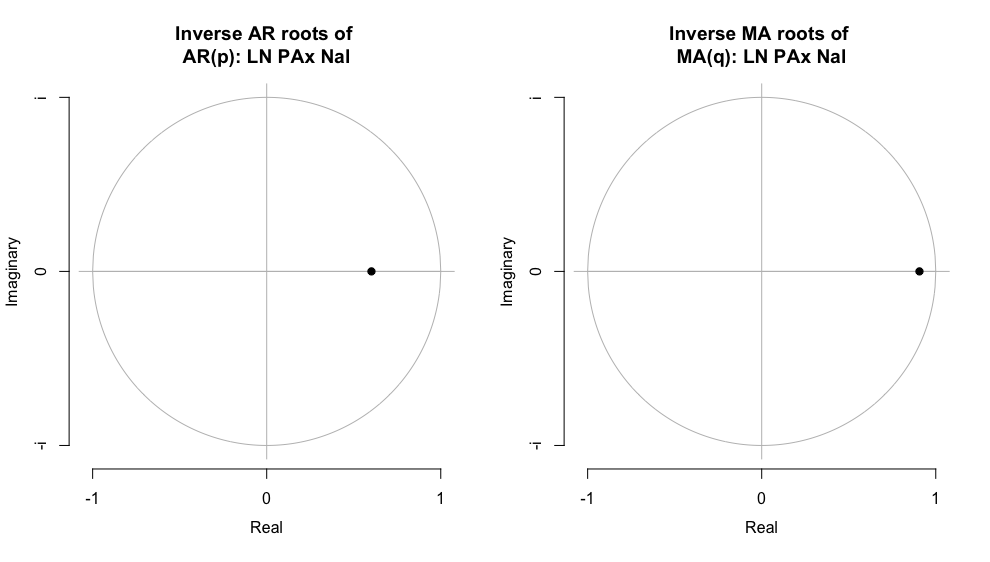
\includegraphics[width=0.95\linewidth]{Plots/G_Roots_ARMA11} 

}

\caption{Inveso de las Raíces del polinomio característico de un ARMA(1,1)}\label{fig:fig412}
\end{figure}

\begin{Shaded}
\begin{Highlighting}[]
\NormalTok{knitr}\SpecialCharTok{::}\FunctionTok{include\_graphics}\NormalTok{(}\StringTok{"Plots/G\_Residuals\_ARMA11.png"}\NormalTok{) }
\end{Highlighting}
\end{Shaded}

\begin{figure}

{\centering 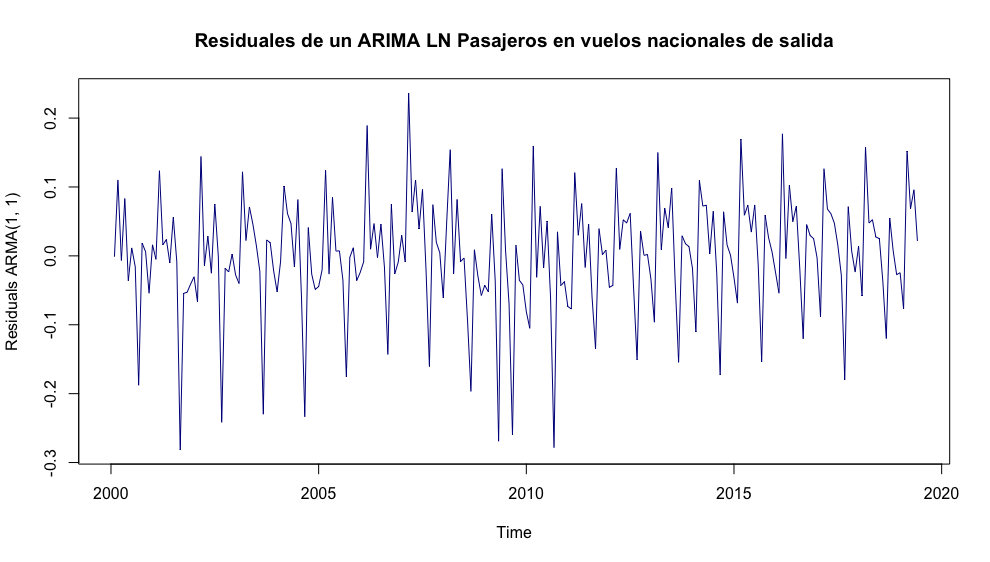
\includegraphics[width=0.95\linewidth]{Plots/G_Residuals_ARMA11} 

}

\caption{Residuales de un $ARMA(1, 1)$ de la serie $DLPaxNal_t$}\label{fig:fig413}
\end{figure}

En lo que resta de este capítulo, utilizaremos la serie en diferencias logarítmicas de los pasajeros en vuelos nacionales de salida, \(DLPaxNal_t\), para discutir los ejemplos que ilustran cada uno de los puntos teóricos que a continuación exponemos.

\hypertarget{funciuxf3n-de-autocorrelaciuxf3n-parcial}{%
\section{Función de Autocorrelación Parcial}\label{funciuxf3n-de-autocorrelaciuxf3n-parcial}}

Ahora introduciremos el concepto de Función de Autocorrelación Parcial (PACF, por sus siglas en inglés). Primero, dadas las condiciones de estabilidad y de convergencia, si suponemos que los procesos AR, MA, ARMA o ARIMA tienen toda la información de los rezagos de la serie en conjunto y toda la información de los promedios móviles del término de error, resulta importante construir una métrica para distinguir el efecto de \(X_{t - \tau}\) o el efecto de \(U_{t - \tau}\) (para cualquier \(\tau\)) sobre \(X_t\) de forma individual.

La idea es construir una métrica de la correlación que existe entre las diferentes variables aleatorias, si para tal efecto se ha controlado el efecto del resto de la información. Así, podemos definir la ecuación que puede responder a este planteamiento como:
\begin{equation}
    X_t = \phi_{k1} X_{t-1} + \phi_{k2} X_{t-2} + \ldots + \phi_{kk} X_{t-k} + U_t
    \label{eq:PACFEq}
\end{equation}

Donde \(\phi_{ki}\) es el coeficiente de la variable dada con el rezago \(i\) si el proceso tiene un órden \(k\). Así, los coeficientes \(\phi_{kk}\) son los coeficientes de la autocorrelación parcial (considerando un proceso AR(k)). Observemos que la autocorrelación parcial mide la correlación entre \(X_t\) y \(X_{t-k}\) que se mantiene cuando el efecto de las variables \(X_{t-1}\), \(X_{t-2}\), \(\ldots\) y \(X_{t-k-1}\) en \(X_{t}\) y \(X_{t-k}\) ha sido eliminado.

Dada la expresión considerada en la ecuación \eqref{eq:PACFEq}, podemos resolver el problema de establecer el valor de cada \(\phi_{ki}\) mediante la solución del sistema que se representa en lo siguiente:
\begin{equation}
    \left[ 
    \begin{array}{c}
        \rho(1) \\
        \rho(2) \\
        \vdots \\
        \rho(k)
    \end{array} 
    \right]
    = 
    \left[ 
    \begin{array}{c c c c}
        1 & \rho(1) & \ldots & \rho(k - 1)\\
        \rho(1) & 1 & \ldots & \rho(k - 2)\\
        \rho(2) & \rho(1) & \ldots & \rho(k - 3)\\
        \vdots & \vdots & \ldots & \vdots\\
        \rho(k - 1) & \rho(k - 2) & \ldots & 1\\
    \end{array} 
    \right]
    \left[ 
    \begin{array}{c}
        \phi_{k1} \\
        \phi_{k2} \\
        \phi_{k3} \\
        \vdots \\
        \phi_{kk} \\
    \end{array} 
    \right]
\end{equation}

Del cual se puede derivar una solución, resolviendo por cualquier método que consideremos y que permita calcular la solución de sistemas de ecuaciones.

Posterior al planteamiento analítico, plantearemos un enfoque para interpretar las funciones de autocorrelación y autocorrelación parcial. Este enfoque pretende aportar al principio de parsimonia, en el cual podemos identificar el número de parámetros que posiblemente puede describir mejor a la serie en un modelo ARMA(p, q).

En el siguiente cuadro mostramos un resumen de las características que debemos observar para determinar el número de parámetros de cada uno de los componentes AR y MA. Lo anterior por observación de las funciones de autocorrelación y autocorrelación parcial. Este enfoque no es el más formal, más adelante implementaremos uno más formal y que puede ser más claro de cómo determinar el número de parámetros.

\begin{longtable}[]{@{}
  >{\centering\arraybackslash}p{(\columnwidth - 4\tabcolsep) * \real{0.3333}}
  >{\centering\arraybackslash}p{(\columnwidth - 4\tabcolsep) * \real{0.3333}}
  >{\centering\arraybackslash}p{(\columnwidth - 4\tabcolsep) * \real{0.3333}}@{}}
\caption{\label{tab:AcAcp} Relación entre la Función de Autocorrelación y la Función de Autocorrelación Parcial de una serie \(X_t\).}\tabularnewline
\toprule\noalign{}
\begin{minipage}[b]{\linewidth}\centering
Modelo
\end{minipage} & \begin{minipage}[b]{\linewidth}\centering
Función de Autocorrelación
\end{minipage} & \begin{minipage}[b]{\linewidth}\centering
Función de Autocorrelación Parcial
\end{minipage} \\
\midrule\noalign{}
\endfirsthead
\toprule\noalign{}
\begin{minipage}[b]{\linewidth}\centering
Modelo
\end{minipage} & \begin{minipage}[b]{\linewidth}\centering
Función de Autocorrelación
\end{minipage} & \begin{minipage}[b]{\linewidth}\centering
Función de Autocorrelación Parcial
\end{minipage} \\
\midrule\noalign{}
\endhead
\bottomrule\noalign{}
\endlastfoot
MA(q) & Rompimienttos en la función & No hay rompimientos \\
AR(p) & No hay rompimientos & Rompimienttos en la función \\
\end{longtable}

\textbf{Ejemplo}. Continuando con el ejemplo en la Figura \ref{fig:fig414} mostramos tanto la Función de Autocorrelación como la Función de Autocorrelación Parcial. En esta identificamos que ambas gráficas muestran que el modelo que explica a la variable \(DLPaxNal_t\) tiene tanto componentes AR como MA. Sin embargo, dado lo errático del comportamiento de ambas funciones, resulta complicado determinar cuál sería un buen número de parámetros \(p\) y \(q\) a considerar en el \(ARMA(p,q)\). Por esta razón, a continuación, plantearemos algunas pruebas más formales para determinar dichos parámetros.

\begin{Shaded}
\begin{Highlighting}[]
\NormalTok{knitr}\SpecialCharTok{::}\FunctionTok{include\_graphics}\NormalTok{(}\StringTok{"Plots/G\_ACF\_PACF.png"}\NormalTok{) }
\end{Highlighting}
\end{Shaded}

\begin{figure}

{\centering 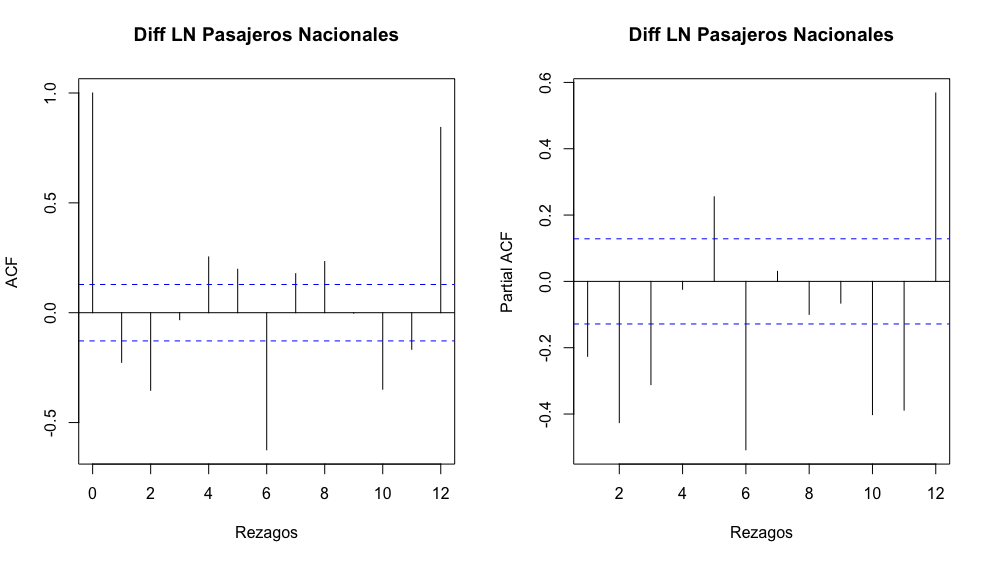
\includegraphics[width=0.95\linewidth]{Plots/G_ACF_PACF} 

}

\caption{Función de Autocorrelación y la Función de Autocorrelación Parcial de una serie $DLPaxNal_t$}\label{fig:fig414}
\end{figure}

\hypertarget{selecciuxf3n-de-las-constantes-p-q-d-en-un-arp-un-maq-un-armap-q-o-un-arimap-d-q}{%
\section{Selección de las constantes p, q, d en un AR(p), un MA(q), un ARMA(p, q) o un ARIMA(p, d, q)}\label{selecciuxf3n-de-las-constantes-p-q-d-en-un-arp-un-maq-un-armap-q-o-un-arimap-d-q}}

Respecto de cómo estimar un proceso ARMA(p, q) --en general utilizaremos este modelo para discutir, pero lo planteado en esta sección es igualmente aplicable en cualquier otro caso como aquellos modelos que incluyen variables exógenas-- existen diversas formas de estimar los parámetros \(a_i\) y \(b_i\): i) por máxima verosimilitud y ii) por mínimos cuadrados ordinarios. El primer caso requiere que conozcamos la distribución del proceso aleatorio \(U_t\). El segundo, por el contrario, no requiere el mismo supuesto. No obstante, para el curso utilizaremos el método de máxima verosimilitud.

Otra duda que debe quedar hasta el momento es ¿cómo determinar el orden \(p\) y \(q\) del proceso ARMA(p, q)? La manera más convencional y formal que existe para tal efecto es utilizar los criterios de información. Así, el orden se elige de acuerdo a aquel criterio de información que resulta ser el mínimo. En el caso de \(d\) se selecciona revisando la gráfica que parezca más estacionaria--más adelante mostraremos un proceso más formal para su selección.

Los criterios de información más comunes son los siguientes:

\begin{enumerate}
\def\labelenumi{\arabic{enumi}.}
\item
  FPE (Final Prediction Error):
  \begin{equation}
   FPE = \frac{T+m}{T-m}\frac{1}{T}\sum_{t=1}^{T} \left( \hat{U}_t^{(p)} \right) ^2
  \end{equation}
\item
  Akaike:
  \begin{equation}
   AIC = ln \left[ \frac{1}{T} \sum_{t=1}^{T} \left( \hat{U}_t^{(p)} \right) ^2 \right] + m \frac{2}{T}
  \end{equation}
\item
  Schwarz:
  \begin{equation}
   SC = ln \left[ \frac{1}{T} \sum_{t=1}^{T} \left( \hat{U}_t^{(p)} \right) ^2 \right] + m \frac{ln(T)}{T}
  \end{equation}
\item
  Hannan - Quinn:
  \begin{equation}
   HQ = ln \left[ \frac{1}{T} \sum_{t=1}^{T} \left( \hat{U}_t^{(p)} \right) ^2 \right] + m \frac{2 ln(ln(T))}{T}
  \end{equation}
\end{enumerate}

Donde \(\hat{U}_t^{(p)}\) son los residuales estimados mediante un proceso ARIMA y \(m\) es el número de parametros estimados: \(m = p + q + 0 + 1\) (ya que asumimos que \(d = 0\)). Una propiedad que no se debe perder de vista es que los criterios de información cumplen la siguiente relación:
\begin{equation}
    orden(SC) \leq orden(HQ) \leq orden(AIC)
\end{equation}

Por esta razón, durante el curso solo utilizaremos el criterio de Akaike para determinar el orden óptimo del proceso ARMA, ya que ello garantiza el orden más grande posible.

\textbf{Ejemplo}. Ahora veamos un ejemplo de estimación del número de rezagos óptimo de un \(ARMA(p, q)\). Retomemos la serie en diferencias logarítmicas de los pasajeros en vuelos nacionales de salidas, pero ahora incluiremos las variables exógenas de dummies estacionales: enero, febrero, julio y diciembre.

Como mencionamos, las gráficas de las funciones de autocorrelación permiten observar el valor de la correlación existente entre la variable en el momento \(t\) con cada uno de los rezagos. Incluso la Función de Autocorrelación Parcial puede ayudar a determinar el número máximo de rezagos que se debe incluir en el proceso \(AR(p)\). No obstante, una métrica más formal es el uso de los criterios de información. En nuestro caso, dado lo discutido, sólo utilizaremos el criterio de Akaike.

Al respecto, en el siguiente cuadro reportamos el criterio de Akaike que resulta de aplicar dicho criterio a los residuales resultantes de cada combinación de procesos \(ARMA(p, q)\). La forma de escoger será aquel modelo que reporta el criterio de Akaike menor. En la cuarta columna de la tabla se señala el valor del criterio de información que resulta ser el mínimo de todos los posibles.

\begin{longtable}[]{@{}ccccc@{}}
\caption{\label{tab:CIARMA} Criterio de Akike para diferentes modelos \(ARMA(p, q)\) de la serie \(DLPaxNal_t\).}\tabularnewline
\toprule\noalign{}
Modelo & AR(p) & MA(p) & Akaike (AIC) & Óptimo \\
\midrule\noalign{}
\endfirsthead
\toprule\noalign{}
Modelo & AR(p) & MA(p) & Akaike (AIC) & Óptimo \\
\midrule\noalign{}
\endhead
\bottomrule\noalign{}
\endlastfoot
1 & 1 & 1 & -475.1190 & \\
2 & 1 & 2 & -473.4397 & \\
3 & 1 & 3 & -483.1239 & \\
4 & 1 & 4 & -482.4932 & \\
5 & 1 & 5 & -506.9880 & \\
6 & 1 & 6 & -533.9411 & \\
7 & 2 & 1 & -473.4758 & \\
\(\vdots\) & \(\vdots\) & \(\vdots\) & \(\vdots\) & \(\vdots\) \\
24 & 4 & 6 & -752.8996 & * \\
\(\vdots\) & \(\vdots\) & \(\vdots\) & \(\vdots\) & \(\vdots\) \\
36 & 6 & 6 & -752.2632 & \\
\end{longtable}

El cuadro anterior reporta un resumen de los resultados para 36 diferentes modelos, todos incluyen variables exógenas. Como resultado del análisis concluimos que el modelo más adecuado es el 24, el cual considera un \(ARMA(4, 6)\), con variables dummies para controlar la estacionalidad de los meses de enero, febrero, julio y diciembre. Más adelante mostramos los resultados del modelo.

No obstante, una inspección de los residuales del modelo nos permite sospechar que requiere de incluir un par de dummies más. Ambas, asociadas con la caída del transporte aéreo en 2009, principalmente asociadas con la crisis mundial de ese año. La Figura \ref{fig:fig415} muestra los residuales mencionados.

\begin{Shaded}
\begin{Highlighting}[]
\NormalTok{knitr}\SpecialCharTok{::}\FunctionTok{include\_graphics}\NormalTok{(}\StringTok{"Plots/G\_Residuals\_ARMA46.png"}\NormalTok{) }
\end{Highlighting}
\end{Shaded}

\begin{figure}

{\centering 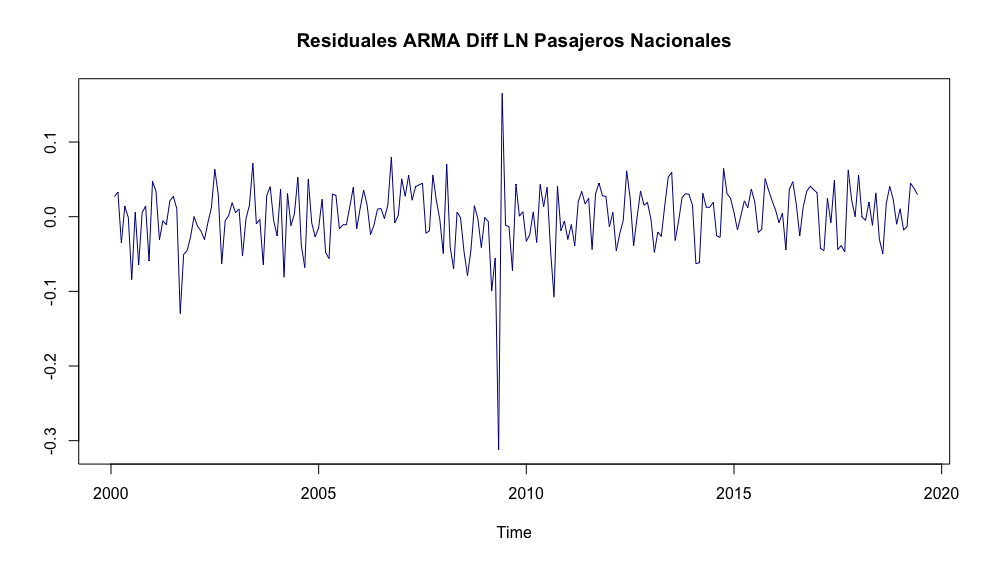
\includegraphics[width=0.95\linewidth]{Plots/G_Residuals_ARMA46} 

}

\caption{Residuales del ARMA(4, 6) de una serie $DLPaxNal_t$}\label{fig:fig415}
\end{figure}

Una vez incluidas dos dummies más para mayo y junio de 2009, analizamos un total de 36 modelos ARMA y determinamos que el orden que minimiza el criterio de Akaike es un \(ARMA(4, 6)\). El siguiente cuadro muestra los resultados para este nuevo modelo. No lo motramos en esta sección, pero ambos modelos reportados tienen raices de sus respectivos polinomios característicos menores a 1 en valor absoluto. En la Figura \ref{fig:fig416} mostramos los residuales ahora ajustados por las dummies de mayo y junio de 2009.

\begin{longtable}[]{@{}ccccc@{}}
\caption{\label{tab:ARMApq} Modelo \(ARMA(p, q)\) de la serie \(DLPaxNal_t\).}\tabularnewline
\toprule\noalign{}
Variable & Coeficiente & Error Est. & Coeficiente & Error Est. \\
\midrule\noalign{}
\endfirsthead
\toprule\noalign{}
Variable & Coeficiente & Error Est. & Coeficiente & Error Est. \\
\midrule\noalign{}
\endhead
\bottomrule\noalign{}
\endlastfoot
& Modelo 1 & Modelo 2 & & \\
Constante & 0.0134 & 0.0033 & 0.0145 & 0.0029 \\
\(DLPaxNal_{t-1}\) & 0.0004 & 0.0011 & 0.0014 & 0.0016 \\
\(DLPaxNal_{t-2}\) & 0.9997 & 0.0019 & 0.9988 & 0.0024 \\
\(DLPaxNal_{t-3}\) & 0.0001 & 0.0012 & 0.0002 & 0.0014 \\
\(DLPaxNal_{t-4}\) & -0.9997 & 0.0004 & -0.9993 & 0.0009 \\
\(\hat{U}_{t-1}\) & -0.2877 & 0.0670 & -0.1472 & 0.0633 \\
\(\hat{U}_{t-2}\) & -1.2028 & 0.0608 & -1.3323 & 0.0625 \\
\(\hat{U}_{t-3}\) & 0.2302 & 0.0765 & 0.1201 & 0.0756 \\
\(\hat{U}_{t-4}\) & 1.2085 & 0.0645 & 1.3142 & 0.0642 \\
\(\hat{U}_{t-5}\) & -0.2634 & 0.0708 & -0.1034 & 0.0717 \\
\(\hat{U}_{t-6}\) & -0.2171 & 0.0606 & -0.3864 & 0.0657 \\
\(DEne_{t}\) & -0.2904 & 0.0172 & -0.2865 & 0.0156 \\
\(DFeb_{t}\) & -0.1312 & 0.0170 & -0.1273 & 0.0140 \\
\(DJul_{t}\) & 0.3303 & 0.0173 & 0.3164 & 0.0156 \\
\(Dic_{t}\) & -0.0118 & 0.0169 & -0.0138 & 0.0137 \\
\(DMay2009_{t}\) & & & -0.3378 & 0.0360 \\
\(DJun2009_{t}\) & & & 0.2371 & 0.0359 \\
\(\hat{\sigma}^2\) & 0.001841 & & 0.001283 & \\
AIC & -752.9 & & -835.73 & \\
\end{longtable}

\begin{Shaded}
\begin{Highlighting}[]
\NormalTok{knitr}\SpecialCharTok{::}\FunctionTok{include\_graphics}\NormalTok{(}\StringTok{"Plots/G\_Residuals\_ARMA46\_D.png"}\NormalTok{) }
\end{Highlighting}
\end{Shaded}

\begin{figure}

{\centering 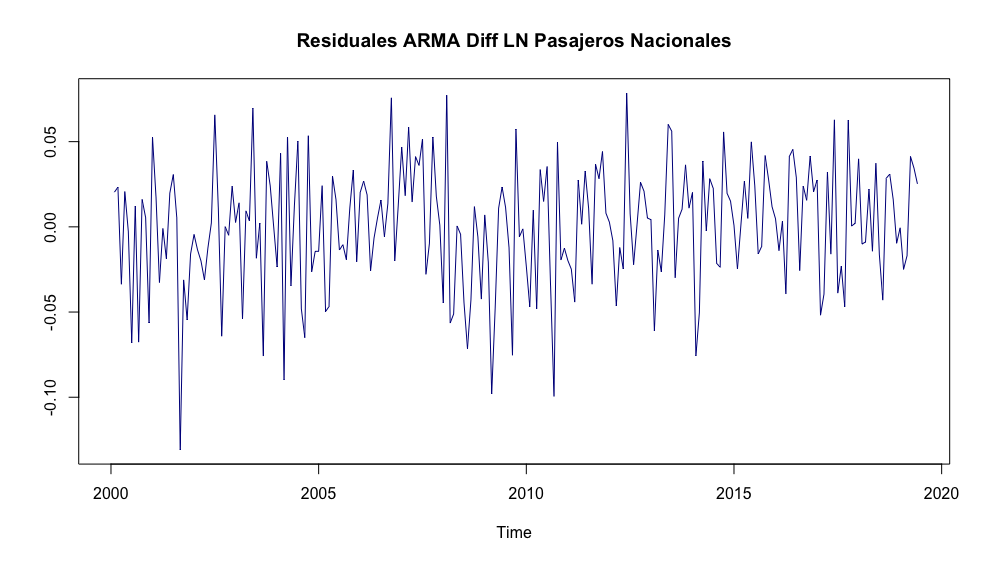
\includegraphics[width=0.95\linewidth]{Plots/G_Residuals_ARMA46_D} 

}

\caption{Residuales del ARMA(4, 6) de una serie $DLPaxNal_t$}\label{fig:fig416}
\end{figure}

\hypertarget{pronuxf3sticos}{%
\section{Pronósticos}\label{pronuxf3sticos}}

Para pronósticar el valor de la serie es necesario determinar cuál es el valor esperado de la serie en un momento \(t + \tau\) condicional en que ésta se comporta como un \(AR(p)\), un \(MA(q)\) o un \(ARMA(p, q)\) y a que los valores antes de \(t\) están dados. Por lo que el pronóstico de la serie estará dado por una expresión:
\begin{eqnarray}
    \mathbb{E}_t[X_{t+\tau}] = \delta + a_1 \mathbb{E}_t[X_{t+\tau-1}] + a_2 \mathbb{E}_t[X_{t+\tau-2}] + \ldots + + a_p \mathbb{E}_t[X_{t+\tau-p}]
    \label{eq:ARMApqFor}
\end{eqnarray}

Lo anterior para todo \(\tau = 0, 1, 2, \ldots\) y considerando que los componentes MA(q) en la ecuación \eqref{eq:ARMApqFor} son cero dado que para todo valor \(t + \tau\) es cierto que \(\mathbb{E}_t[U_{t+\tau}]\).

Continuando con el ejemplo, en la Figura \ref{fig:fig417} mostramos el resultado del pronóstico de la serie a partir del modelo ARMA(4, 6) que hemos discutido anteriormente.

\begin{Shaded}
\begin{Highlighting}[]
\FunctionTok{library}\NormalTok{(ggplot2)}
\FunctionTok{library}\NormalTok{(dplyr)}
\FunctionTok{library}\NormalTok{(readxl)}
\FunctionTok{library}\NormalTok{(stats)}

\NormalTok{Datos }\OtherTok{\textless{}{-}} \FunctionTok{read\_excel}\NormalTok{(}\StringTok{"BD/Base\_Transporte\_ARIMA.xlsx"}\NormalTok{, }
                    \AttributeTok{sheet =} \StringTok{"Datos"}\NormalTok{, }\AttributeTok{col\_names =} \ConstantTok{TRUE}\NormalTok{)}

\NormalTok{Pax\_Nal }\OtherTok{\textless{}{-}} \FunctionTok{ts}\NormalTok{(Datos}\SpecialCharTok{$}\NormalTok{Pax\_Nal, }
              \AttributeTok{start =} \FunctionTok{c}\NormalTok{(}\DecValTok{2000}\NormalTok{, }\DecValTok{1}\NormalTok{), }
              \AttributeTok{freq =} \DecValTok{12}\NormalTok{)}

\NormalTok{LPax\_Nal }\OtherTok{\textless{}{-}} \FunctionTok{ts}\NormalTok{(}\FunctionTok{log}\NormalTok{(Datos}\SpecialCharTok{$}\NormalTok{Pax\_Nal), }
               \AttributeTok{start =} \FunctionTok{c}\NormalTok{(}\DecValTok{2000}\NormalTok{, }\DecValTok{1}\NormalTok{), }
               \AttributeTok{freq =} \DecValTok{12}\NormalTok{)}

\NormalTok{DLPax\_Nal }\OtherTok{\textless{}{-}} \FunctionTok{ts}\NormalTok{(}\FunctionTok{log}\NormalTok{(Datos}\SpecialCharTok{$}\NormalTok{Pax\_Nal) }\SpecialCharTok{{-}} \FunctionTok{lag}\NormalTok{(}\FunctionTok{log}\NormalTok{(Datos}\SpecialCharTok{$}\NormalTok{Pax\_Nal), }\DecValTok{1}\NormalTok{),}
                \AttributeTok{start =} \FunctionTok{c}\NormalTok{(}\DecValTok{2000}\NormalTok{, }\DecValTok{1}\NormalTok{), }
                \AttributeTok{freq =} \DecValTok{12}\NormalTok{)}

\NormalTok{D\_Mar2020   }\OtherTok{\textless{}{-}} \FunctionTok{ts}\NormalTok{(Datos}\SpecialCharTok{$}\NormalTok{D\_Mar2020, }
                \AttributeTok{start =} \FunctionTok{c}\NormalTok{(}\DecValTok{2000}\NormalTok{, }\DecValTok{1}\NormalTok{), }
                \AttributeTok{freq =} \DecValTok{12}\NormalTok{)}

\NormalTok{D\_Abr2020   }\OtherTok{\textless{}{-}} \FunctionTok{ts}\NormalTok{(Datos}\SpecialCharTok{$}\NormalTok{D\_Abr2020, }
                \AttributeTok{start =} \FunctionTok{c}\NormalTok{(}\DecValTok{2000}\NormalTok{, }\DecValTok{1}\NormalTok{), }
                \AttributeTok{freq =} \DecValTok{12}\NormalTok{)}

\NormalTok{D\_Jun2020   }\OtherTok{\textless{}{-}} \FunctionTok{ts}\NormalTok{(Datos}\SpecialCharTok{$}\NormalTok{D\_Jun2020, }
                \AttributeTok{start =} \FunctionTok{c}\NormalTok{(}\DecValTok{2000}\NormalTok{, }\DecValTok{1}\NormalTok{), }
                \AttributeTok{freq =} \DecValTok{12}\NormalTok{)}

\NormalTok{D\_Jul2020 }\OtherTok{\textless{}{-}} \FunctionTok{ts}\NormalTok{(Datos}\SpecialCharTok{$}\NormalTok{D\_Jul2020, }
                \AttributeTok{start =} \FunctionTok{c}\NormalTok{(}\DecValTok{2000}\NormalTok{, }\DecValTok{1}\NormalTok{), }
                \AttributeTok{freq =} \DecValTok{12}\NormalTok{)}

\NormalTok{D\_Mar2021 }\OtherTok{\textless{}{-}} \FunctionTok{ts}\NormalTok{(Datos}\SpecialCharTok{$}\NormalTok{D\_Mar2021, }
                \AttributeTok{start =} \FunctionTok{c}\NormalTok{(}\DecValTok{2000}\NormalTok{, }\DecValTok{1}\NormalTok{), }
                \AttributeTok{freq =} \DecValTok{12}\NormalTok{)}

\NormalTok{D\_Ene }\OtherTok{\textless{}{-}} \FunctionTok{ts}\NormalTok{(Datos}\SpecialCharTok{$}\NormalTok{D\_Ene, }
            \AttributeTok{start =} \FunctionTok{c}\NormalTok{(}\DecValTok{2000}\NormalTok{, }\DecValTok{1}\NormalTok{), }
            \AttributeTok{freq =} \DecValTok{12}\NormalTok{)}

\NormalTok{D\_Feb }\OtherTok{\textless{}{-}} \FunctionTok{ts}\NormalTok{(Datos}\SpecialCharTok{$}\NormalTok{D\_Feb, }
            \AttributeTok{start =} \FunctionTok{c}\NormalTok{(}\DecValTok{2000}\NormalTok{, }\DecValTok{1}\NormalTok{), }
            \AttributeTok{freq =} \DecValTok{12}\NormalTok{)}

\NormalTok{D\_Jul }\OtherTok{\textless{}{-}} \FunctionTok{ts}\NormalTok{(Datos}\SpecialCharTok{$}\NormalTok{D\_Jul, }
            \AttributeTok{start =} \FunctionTok{c}\NormalTok{(}\DecValTok{2000}\NormalTok{, }\DecValTok{1}\NormalTok{), }
            \AttributeTok{freq =} \DecValTok{12}\NormalTok{)}

\NormalTok{D\_Dic }\OtherTok{\textless{}{-}} \FunctionTok{ts}\NormalTok{(Datos}\SpecialCharTok{$}\NormalTok{D\_Dic, }
            \AttributeTok{start =} \FunctionTok{c}\NormalTok{(}\DecValTok{2000}\NormalTok{, }\DecValTok{1}\NormalTok{), }
            \AttributeTok{freq =} \DecValTok{12}\NormalTok{)}

\NormalTok{ARMA\_Ex\_DLPax\_Nal\_2 }\OtherTok{\textless{}{-}} \FunctionTok{arima}\NormalTok{(DLPax\_Nal, }\AttributeTok{order =} \FunctionTok{c}\NormalTok{(}\DecValTok{6}\NormalTok{, }\DecValTok{0}\NormalTok{, }\DecValTok{6}\NormalTok{),}
                             \AttributeTok{xreg =} \FunctionTok{cbind}\NormalTok{(D\_Ene, D\_Feb, D\_Jul, }
\NormalTok{                                          D\_Dic, D\_Mar2020, }
\NormalTok{                                          D\_Abr2020, D\_Jun2020, }
\NormalTok{                                          D\_Jul2020, D\_Mar2021),}
                             \AttributeTok{method =} \StringTok{"ML"}\NormalTok{)}

\NormalTok{Predict\_Datos }\OtherTok{\textless{}{-}} \FunctionTok{read\_excel}\NormalTok{(}\StringTok{"BD/Predict\_Base\_Transporte\_ARIMA.xlsx"}\NormalTok{, }
                            \AttributeTok{sheet =} \StringTok{"Datos"}\NormalTok{, }\AttributeTok{col\_names =} \ConstantTok{TRUE}\NormalTok{)}

\NormalTok{D\_Mar2020\_f }\OtherTok{\textless{}{-}} \FunctionTok{ts}\NormalTok{(Predict\_Datos}\SpecialCharTok{$}\NormalTok{D\_Mar2020, }
                \AttributeTok{start =} \FunctionTok{c}\NormalTok{(}\DecValTok{2025}\NormalTok{, }\DecValTok{7}\NormalTok{), }
                \AttributeTok{freq =} \DecValTok{12}\NormalTok{)}

\NormalTok{D\_Abr2020\_f }\OtherTok{\textless{}{-}} \FunctionTok{ts}\NormalTok{(Predict\_Datos}\SpecialCharTok{$}\NormalTok{D\_Abr2020, }
                \AttributeTok{start =} \FunctionTok{c}\NormalTok{(}\DecValTok{2025}\NormalTok{, }\DecValTok{7}\NormalTok{), }
                \AttributeTok{freq =} \DecValTok{12}\NormalTok{)}

\NormalTok{D\_Jun2020\_f }\OtherTok{\textless{}{-}} \FunctionTok{ts}\NormalTok{(Predict\_Datos}\SpecialCharTok{$}\NormalTok{D\_Jun2020, }
                \AttributeTok{start =} \FunctionTok{c}\NormalTok{(}\DecValTok{2025}\NormalTok{, }\DecValTok{7}\NormalTok{), }
                \AttributeTok{freq =} \DecValTok{12}\NormalTok{)}

\NormalTok{D\_Jul2020\_f }\OtherTok{\textless{}{-}} \FunctionTok{ts}\NormalTok{(Predict\_Datos}\SpecialCharTok{$}\NormalTok{D\_Jul2020, }
                \AttributeTok{start =} \FunctionTok{c}\NormalTok{(}\DecValTok{2025}\NormalTok{, }\DecValTok{7}\NormalTok{), }
                \AttributeTok{freq =} \DecValTok{12}\NormalTok{)}

\NormalTok{D\_Mar2021\_f }\OtherTok{\textless{}{-}} \FunctionTok{ts}\NormalTok{(Predict\_Datos}\SpecialCharTok{$}\NormalTok{D\_Mar2021, }
                \AttributeTok{start =} \FunctionTok{c}\NormalTok{(}\DecValTok{2025}\NormalTok{, }\DecValTok{7}\NormalTok{), }
                \AttributeTok{freq =} \DecValTok{12}\NormalTok{)}

\NormalTok{D\_Ene\_f }\OtherTok{\textless{}{-}} \FunctionTok{ts}\NormalTok{(Predict\_Datos}\SpecialCharTok{$}\NormalTok{D\_Ene, }
            \AttributeTok{start =} \FunctionTok{c}\NormalTok{(}\DecValTok{2025}\NormalTok{, }\DecValTok{7}\NormalTok{), }
            \AttributeTok{freq =} \DecValTok{12}\NormalTok{)}

\NormalTok{D\_Feb\_f }\OtherTok{\textless{}{-}} \FunctionTok{ts}\NormalTok{(Predict\_Datos}\SpecialCharTok{$}\NormalTok{D\_Feb, }
            \AttributeTok{start =} \FunctionTok{c}\NormalTok{(}\DecValTok{2025}\NormalTok{, }\DecValTok{7}\NormalTok{), }
            \AttributeTok{freq =} \DecValTok{12}\NormalTok{)}

\NormalTok{D\_Jul\_f }\OtherTok{\textless{}{-}} \FunctionTok{ts}\NormalTok{(Predict\_Datos}\SpecialCharTok{$}\NormalTok{D\_Jul, }
           \AttributeTok{start =} \FunctionTok{c}\NormalTok{(}\DecValTok{2025}\NormalTok{, }\DecValTok{7}\NormalTok{), }
            \AttributeTok{freq =} \DecValTok{12}\NormalTok{)}

\NormalTok{D\_Dic\_f }\OtherTok{\textless{}{-}} \FunctionTok{ts}\NormalTok{(Predict\_Datos}\SpecialCharTok{$}\NormalTok{D\_Dic, }
            \AttributeTok{start =} \FunctionTok{c}\NormalTok{(}\DecValTok{2025}\NormalTok{, }\DecValTok{7}\NormalTok{), }
            \AttributeTok{freq =} \DecValTok{12}\NormalTok{)}

\NormalTok{DLPax\_Nal\_f }\OtherTok{\textless{}{-}} \FunctionTok{predict}\NormalTok{(ARMA\_Ex\_DLPax\_Nal\_2, }\AttributeTok{n.ahead =} \DecValTok{24}\NormalTok{, }
                      \AttributeTok{newxreg =} \FunctionTok{cbind}\NormalTok{(D\_Ene\_f, D\_Feb\_f, D\_Jul\_f, }
\NormalTok{                                      D\_Dic\_f, D\_Mar2020\_f, }
\NormalTok{                                      D\_Abr2020\_f, D\_Jun2020\_f, }
\NormalTok{                                      D\_Jul2020\_f, D\_Mar2021\_f))}

\NormalTok{Pronostico\_Arima }\OtherTok{\textless{}{-}} \FunctionTok{read\_excel}\NormalTok{(}\StringTok{"BD/Pronostico\_Arima.xlsx"}\NormalTok{, }
                               \AttributeTok{sheet =} \StringTok{"Datos"}\NormalTok{, }\AttributeTok{col\_names =} \ConstantTok{TRUE}\NormalTok{)}

\NormalTok{Pronostico\_Arima}\SpecialCharTok{$}\NormalTok{Pax\_Nal\_f }\OtherTok{\textless{}{-}}\NormalTok{ Pronostico\_Arima}\SpecialCharTok{$}\NormalTok{Pax\_Nal}

\ControlFlowTok{for}\NormalTok{(i }\ControlFlowTok{in} \DecValTok{1}\SpecialCharTok{:}\DecValTok{24}\NormalTok{)\{}
\NormalTok{  Pronostico\_Arima}\SpecialCharTok{$}\NormalTok{Pax\_Nal\_f[}\DecValTok{306} \SpecialCharTok{+}\NormalTok{ i] }\OtherTok{\textless{}{-}} 
\NormalTok{    Pronostico\_Arima}\SpecialCharTok{$}\NormalTok{Pax\_Nal\_f[}\DecValTok{306} \SpecialCharTok{+}\NormalTok{ i }\SpecialCharTok{{-}} \DecValTok{1}\NormalTok{]}\SpecialCharTok{*}\NormalTok{(}\DecValTok{1} \SpecialCharTok{+}\NormalTok{ DLPax\_Nal\_f}\SpecialCharTok{$}\NormalTok{pred[i])}
\NormalTok{\}}

\FunctionTok{options}\NormalTok{(}\AttributeTok{scipen =} \DecValTok{999}\NormalTok{) }\CommentTok{\# NO notacion cientifica}

\FunctionTok{ggplot}\NormalTok{(}\AttributeTok{data =}\NormalTok{ Pronostico\_Arima, }\FunctionTok{aes}\NormalTok{(}\AttributeTok{x =}\NormalTok{ Periodo)) }\SpecialCharTok{+}
  \FunctionTok{geom\_line}\NormalTok{(}\FunctionTok{aes}\NormalTok{(}\AttributeTok{y =}\NormalTok{ Pax\_Nal\_f, }\AttributeTok{color =} \StringTok{"Pax\_Nal\_f"}\NormalTok{)) }\SpecialCharTok{+}
  \FunctionTok{geom\_line}\NormalTok{(}\FunctionTok{aes}\NormalTok{(}\AttributeTok{y =}\NormalTok{ Pax\_Nal, }\AttributeTok{color =} \StringTok{"Pax\_Nal"}\NormalTok{)) }\SpecialCharTok{+}
  \FunctionTok{scale\_color\_brewer}\NormalTok{(}\AttributeTok{type =} \StringTok{"qual"}\NormalTok{, }\AttributeTok{palette =} \DecValTok{2}\NormalTok{) }\SpecialCharTok{+}
  \CommentTok{\#theme\_bw() + }
  \FunctionTok{theme}\NormalTok{(}\AttributeTok{legend.position =} \StringTok{"bottom"}\NormalTok{) }\SpecialCharTok{+}
  \FunctionTok{theme}\NormalTok{(}\AttributeTok{legend.title =} \FunctionTok{element\_blank}\NormalTok{()) }\SpecialCharTok{+}
  \FunctionTok{guides}\NormalTok{(}\AttributeTok{col =} \FunctionTok{guide\_legend}\NormalTok{(}\AttributeTok{nrow =} \DecValTok{1}\NormalTok{, }\AttributeTok{byrow =} \ConstantTok{TRUE}\NormalTok{)) }\SpecialCharTok{+} 
  \FunctionTok{xlab}\NormalTok{(}\StringTok{"Tiempo"}\NormalTok{) }\SpecialCharTok{+} 
  \FunctionTok{ylab}\NormalTok{(}\StringTok{"Pasajeros"}\NormalTok{) }\SpecialCharTok{+} 
  \FunctionTok{theme}\NormalTok{(}\AttributeTok{plot.title =} \FunctionTok{element\_text}\NormalTok{(}\AttributeTok{size =} \DecValTok{11}\NormalTok{, }\AttributeTok{face =} \StringTok{"bold"}\NormalTok{, }
                                  \AttributeTok{hjust =} \DecValTok{0}\NormalTok{)) }\SpecialCharTok{+} 
  \FunctionTok{theme}\NormalTok{(}\AttributeTok{plot.subtitle =} \FunctionTok{element\_text}\NormalTok{(}\AttributeTok{size =} \DecValTok{10}\NormalTok{, }\AttributeTok{hjust =} \DecValTok{0}\NormalTok{)) }\SpecialCharTok{+} 
  \FunctionTok{theme}\NormalTok{(}\AttributeTok{plot.caption =} \FunctionTok{element\_text}\NormalTok{(}\AttributeTok{size =} \DecValTok{10}\NormalTok{, }\AttributeTok{hjust =} \DecValTok{0}\NormalTok{)) }\SpecialCharTok{+}
  \FunctionTok{theme}\NormalTok{(}\AttributeTok{plot.margin =} \FunctionTok{unit}\NormalTok{(}\FunctionTok{c}\NormalTok{(}\DecValTok{1}\NormalTok{,}\DecValTok{1}\NormalTok{,}\DecValTok{1}\NormalTok{,}\DecValTok{1}\NormalTok{), }\StringTok{"cm"}\NormalTok{)) }\SpecialCharTok{+}
  \FunctionTok{labs}\NormalTok{(}
    \AttributeTok{title =} \StringTok{"Pasajeros en vuelos nacionales (Salidas)"}\NormalTok{,}
    \AttributeTok{subtitle =} \StringTok{"(Ene{-}2000 a Jun{-}2019)"}\NormalTok{,}
    \AttributeTok{caption =} \StringTok{"Fuente: Elaboración propia"}
\NormalTok{  )}
\end{Highlighting}
\end{Shaded}

\begin{figure}

{\centering 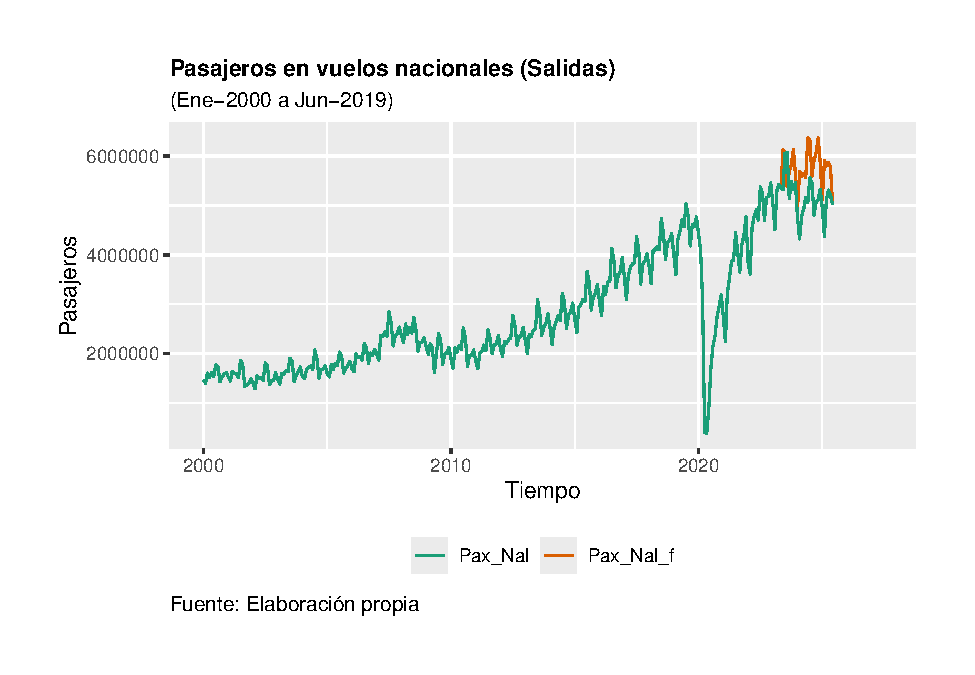
\includegraphics{Notas-Series-Tiempo_files/figure-latex/fig417-1} 

}

\caption{Pronóstico de la serie $PaxNAl_t$ a partir de una ARMA(4,6) en diferencias logaritmicas}\label{fig:fig417}
\end{figure}

\begin{Shaded}
\begin{Highlighting}[]
\FunctionTok{ggsave}\NormalTok{(}\StringTok{"Pax\_Nal\_f.png"}\NormalTok{, }\AttributeTok{width =} \DecValTok{20}\NormalTok{, }\AttributeTok{height =} \DecValTok{15}\NormalTok{, }\AttributeTok{units =} \StringTok{"cm"}\NormalTok{)}
\end{Highlighting}
\end{Shaded}

\hypertarget{desestacionalizaciuxf3n-y-filtrado-de-series}{%
\section{Desestacionalización y filtrado de Series}\label{desestacionalizaciuxf3n-y-filtrado-de-series}}

\hypertarget{motivaciuxf3n}{%
\section{Motivación}\label{motivaciuxf3n}}

Existen múltiples enfoques para la desestacionalización de series. Algunos modelos, por ejemplo, pueden estar basados en modelos ARIMA como un conjunto de dummies. No obstante, en el caso particular que discutiremos en este curso, estará basado en un modelo ARIMA de la serie. Este enfoque está basado en el modelo X11 de la oficina del censo de Estados Unidos (Census Bureau) el cual es conocido como el modelo X13-ARIMA-SEATS.\footnote{ La información y material respecto del modelo esta disponible en la dirección \url{https://www.census.gov/srd/www/x13as/}} El modelo X13-ARIMA-SEATS es, como su nombre lo indica, la combinación de un modelo ARIMA con componentes estacionales (por la traducción literal de la palabra: seasonal).

Un modelo ARIMA estacional emplea la serie en diferencias y como regresores los valores rezagados de las diferencias de la serie tantas veces como procesos estacionales \(s\) existan en ésta, con el objeto de remover los efectos aditivos de la estacionalidad. Sólo para entender qué significa este mecanismo, recordemos que cuando se utiliza la primera diferencia de la serie respecto del periodo inmediato anterior se remueve la tendencia. Por su parte, cuando se incluye la diferencia respecto del mes \(s\) se está en el caso en que se modela la serie como una media móvil en términos del rezago \(s\).

El modelo ARIMA estacional incluye como componentes autorregresivos y de medias móviles a los valores rezagados de la serie en el periodo \(s\) en diferencias. El ARIMA(p, d, q)(P, D, Q) estacional puede ser expresado de la siguiente manera utilizando el operador rezago \(L\):
\begin{equation}
    \Theta_P(L^s) \theta_p(L) (1 - L^s)^D (1 - L)^d X_t = \Psi_Q(L^s) \psi_q(L) U_t
    \label{eq:ARIMAseas}
\end{equation}

Donde \(\Theta_P(.)\), \(\theta_p(.)\), \(\Psi_Q(.)\) y \(\psi_q(.)\) son polinomios de \(L\) de orden \(P\), \(p\), \(Q\) y \(q\) respectivamente. En general, la representación es de una serie no estacionaria, aunque si \(D = d = 0\) y las raíces del polinomio característico (de los polinomios del lado izquierdo de la ecuación \eqref{eq:ARIMAseas} todas son más grandes que 1 en valor absoluto, el proceso modelado será estacionario.

Si bien es cierto que existen otras formas de modelar la desestacionalización, como la modelación en diferencias con dummies para identificar ciertos patrones regulares, en los algoritmos disponibles como el X11 o X13-ARIMA-SEATS se emplea la formulación de la ecuación \eqref{eq:ARIMAseas}. A continuación, implementaremos la desestacionalización de una serie.

Como ejemplo utilizaremos la serie del Índice Nacional de Precios al Consumidor (INPC).\footnote{Las definiciones de las variables ocupadas es:
* INPC: Indice Nacional de Precios al Consumidor (2QJul2018 = 100)
* TC: Tipo de Cambio FIX 
* CETE28: Tasa de rendimiento promedio mensual de los Cetes 28, en por ciento anual
* IGAE: Indicador global de la actividad económica (2013 = 100)
* IPI: Industrial Production Index (2012 = 100)
} Podemos ver que la serie original del INPC y su ajuste estacional bajo una metodología X13-ARIMA-SEATS son como se muestra en la Figura \ref{fig:fig51}.

\begin{Shaded}
\begin{Highlighting}[]
\FunctionTok{library}\NormalTok{(ggplot2)}
\FunctionTok{library}\NormalTok{(dplyr)}
\FunctionTok{library}\NormalTok{(readxl)}
\FunctionTok{library}\NormalTok{(stats)}
\FunctionTok{library}\NormalTok{(seasonal)}
\end{Highlighting}
\end{Shaded}

\begin{verbatim}
## 
## Attaching package: 'seasonal'
\end{verbatim}

\begin{verbatim}
## The following object is masked from 'package:tibble':
## 
##     view
\end{verbatim}

\begin{Shaded}
\begin{Highlighting}[]
\FunctionTok{library}\NormalTok{(seasonalview)}
\end{Highlighting}
\end{Shaded}

\begin{verbatim}
## 
## Attaching package: 'seasonalview'
\end{verbatim}

\begin{verbatim}
## The following object is masked from 'package:seasonal':
## 
##     view
\end{verbatim}

\begin{verbatim}
## The following object is masked from 'package:tibble':
## 
##     view
\end{verbatim}

\begin{Shaded}
\begin{Highlighting}[]
\FunctionTok{library}\NormalTok{(shiny)}

\NormalTok{Datos }\OtherTok{\textless{}{-}} \FunctionTok{read\_excel}\NormalTok{(}\StringTok{"BD/Base\_VAR.xlsx"}\NormalTok{, }\AttributeTok{sheet =} \StringTok{"Datos"}\NormalTok{, }\AttributeTok{col\_names =} \ConstantTok{TRUE}\NormalTok{)}

\NormalTok{INPC }\OtherTok{\textless{}{-}} \FunctionTok{ts}\NormalTok{(Datos}\SpecialCharTok{$}\NormalTok{INPC, }
           \AttributeTok{start =} \FunctionTok{c}\NormalTok{(}\DecValTok{2000}\NormalTok{, }\DecValTok{1}\NormalTok{), }
           \AttributeTok{freq =} \DecValTok{12}\NormalTok{)}

\NormalTok{Seas\_INPC }\OtherTok{\textless{}{-}} \FunctionTok{seas}\NormalTok{(INPC)}

\NormalTok{INPC\_Ad }\OtherTok{\textless{}{-}} \FunctionTok{final}\NormalTok{(Seas\_INPC)}

\CommentTok{\#names(Seas\_INPC)}

\CommentTok{\#summary(Seas\_INPC)}

\FunctionTok{plot}\NormalTok{(Seas\_INPC)}
\end{Highlighting}
\end{Shaded}

\begin{figure}

{\centering 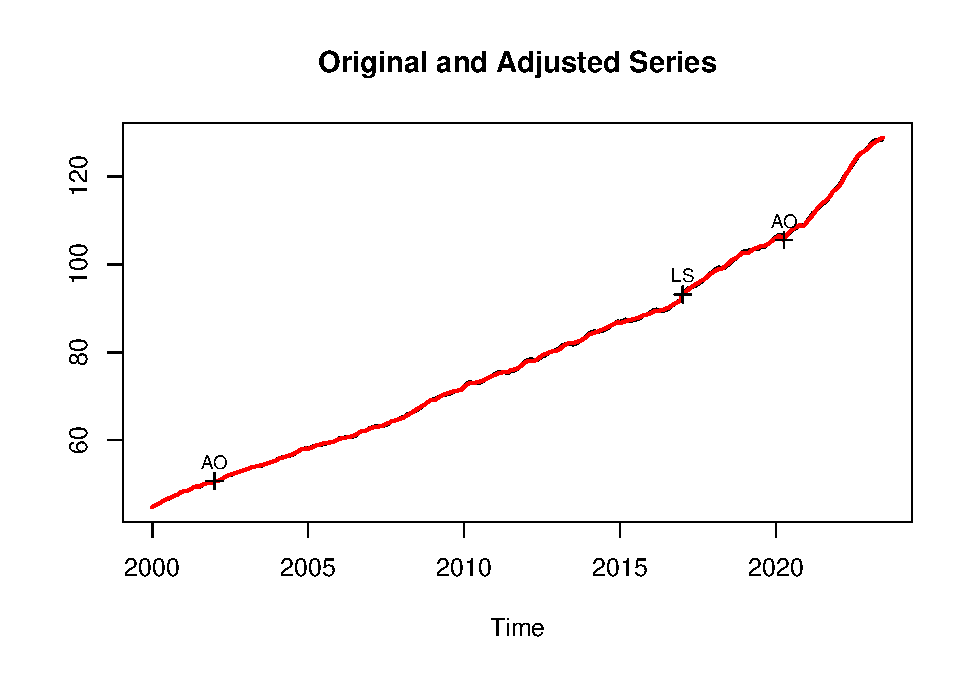
\includegraphics[width=0.95\linewidth]{Notas-Series-Tiempo_files/figure-latex/fig51-1} 

}

\caption{Índice Nacional de Precios al Consumidor ($INPC_t$) y su serie desestacionalizada utilizando un proceso X13-ARIMA-SEATS}\label{fig:fig51}
\end{figure}

\begin{Shaded}
\begin{Highlighting}[]
\CommentTok{\# Forma Facil:}

\CommentTok{\#view(Seas\_INPC)}

\NormalTok{TC }\OtherTok{\textless{}{-}} \FunctionTok{ts}\NormalTok{(Datos}\SpecialCharTok{$}\NormalTok{TC, }
         \AttributeTok{start =} \FunctionTok{c}\NormalTok{(}\DecValTok{2000}\NormalTok{, }\DecValTok{1}\NormalTok{),}
         \AttributeTok{freq =} \DecValTok{12}\NormalTok{)}

\NormalTok{Seas\_TC }\OtherTok{\textless{}{-}} \FunctionTok{seas}\NormalTok{(TC)}

\NormalTok{TC\_Ad }\OtherTok{\textless{}{-}} \FunctionTok{final}\NormalTok{(Seas\_TC)}

\NormalTok{CETE28 }\OtherTok{\textless{}{-}} \FunctionTok{ts}\NormalTok{(Datos}\SpecialCharTok{$}\NormalTok{CETE28, }
             \AttributeTok{start =} \FunctionTok{c}\NormalTok{(}\DecValTok{2000}\NormalTok{, }\DecValTok{1}\NormalTok{), }
             \AttributeTok{freq =} \DecValTok{12}\NormalTok{)}

\NormalTok{Seas\_CETE28 }\OtherTok{\textless{}{-}} \FunctionTok{seas}\NormalTok{(CETE28)}

\NormalTok{CETE28\_Ad }\OtherTok{\textless{}{-}} \FunctionTok{final}\NormalTok{(Seas\_CETE28)}

\NormalTok{IGAE }\OtherTok{\textless{}{-}} \FunctionTok{ts}\NormalTok{(Datos}\SpecialCharTok{$}\NormalTok{IGAE, }
           \AttributeTok{start =} \FunctionTok{c}\NormalTok{(}\DecValTok{2000}\NormalTok{, }\DecValTok{1}\NormalTok{), }
           \AttributeTok{freq =} \DecValTok{12}\NormalTok{)}

\NormalTok{Seas\_IGAE }\OtherTok{\textless{}{-}} \FunctionTok{seas}\NormalTok{(IGAE)}

\NormalTok{IGAE\_Ad }\OtherTok{\textless{}{-}} \FunctionTok{final}\NormalTok{(Seas\_IGAE)}

\NormalTok{IPI }\OtherTok{\textless{}{-}} \FunctionTok{ts}\NormalTok{(Datos}\SpecialCharTok{$}\NormalTok{IPI, }
          \AttributeTok{start =} \FunctionTok{c}\NormalTok{(}\DecValTok{2000}\NormalTok{, }\DecValTok{1}\NormalTok{), }
          \AttributeTok{freq =} \DecValTok{12}\NormalTok{)}

\NormalTok{Seas\_IPI }\OtherTok{\textless{}{-}} \FunctionTok{seas}\NormalTok{(IPI)}

\NormalTok{IPI\_Ad }\OtherTok{\textless{}{-}} \FunctionTok{final}\NormalTok{(Seas\_IPI)}

\NormalTok{Datos\_Ad }\OtherTok{\textless{}{-}} \FunctionTok{data.frame}\NormalTok{(}\FunctionTok{cbind}\NormalTok{(INPC\_Ad, TC\_Ad, CETE28\_Ad, IGAE\_Ad, IPI\_Ad))}

\NormalTok{Datos\_Ad }\OtherTok{\textless{}{-}} \FunctionTok{cbind}\NormalTok{(Datos, Datos\_Ad)}

\FunctionTok{save}\NormalTok{(Datos\_Ad, }\AttributeTok{file =} \StringTok{"BD/Datos\_Ad0.RData"}\NormalTok{)}
\end{Highlighting}
\end{Shaded}

El mismo procesamiento puede ser seguido para todas las series que busquemos analizar. En particular, en adelante, además del INPC que incluimos en la lista, utilizaremos las siguientes series, así como su versión desestacionalizada:

\begin{itemize}
    \item Índice Nacional de Precios al Consumidor (base 2QJul2018 = 100), $INPC_t$.
    \item Tipo de Cambio FIX, $TC_t$
    \item Tasa de rendimiento promedio mensual de los Cetes 28, en por ciento anual, $CETE28_t$
    \item Indicador global de la actividad económica (base 2013 = 100), $IGAE_t$
    \item Industrial Production Index o Índice de Producción Industrial de los Estados Unidos (base 2012 = 100), $IPI_t$
\end{itemize}

\hypertarget{filtro-hodrick-prescott}{%
\section{Filtro Hodrick-Prescott}\label{filtro-hodrick-prescott}}

Como último tema de los procesos univariados y que no necesariamente aplican a series estacionarias, a continuación desarrollaremos el procedimiento conocido como filtro de Hodrick y Prescott (1997). El trabajo de estos autores era determinar una técnica de regresión que permitiera utilizar series agregadas o macroeconómicas para separarlas en dos componentes: uno de ciclo de negocios y otro de tendencia. En su trabajo original, Hodrick y Prescott (1997) utilizaron datos trimestrales de algunas series como el Gross Domestic Product (GNP, por sus siglas en Inglés), los agregados monetarios M1, empleo, etc., de los Estados Unidos que fueron observados posteriormente a la Segunda Guerra Mundial.

El marco conceptual de Hodrick y Prescott (1997) parte de suponer una serie \(X_t\) que se puede descomponer en la suma de componente de crecimiento tendencial, \(g_t\), y su componente de ciclio de negocios, \(c_t\), de esta forma para \(t = 1, 2, \ldots, T\) tenemos que:
\begin{equation}
    X_t = g_t + c_t
    \label{eq:HPEq}
\end{equation}

En la ecuación \eqref{eq:HPEq} se asume que el ajuste de la ruta seguida por \(g_t\) es resultado de la suma de los cuadrados de su segunda diferencia. En esa misma ecuación asumiremos que \(c_t\) son las desviaciones de \(g_t\), las cuales en el largo plazo tienen una media igual a cero (0). Por esta razón, se suele decir que el filtro de Hodrick y Prescott representa una descomposición de la serie en su componente de crecimiento natural y de sus desviaciones transitorias que en promedio son cero, en el largo plazo.

Estas consideraciones que hemos mencionado señalan que el procesimiento de Hodrick y Prescott (1997) implican resolver el siguiente problema minimización para determinar cada uno de los componentes en que \(X_t\) se puede descomponer:
\begin{equation}
    \min_{\{ g_t \}^T_{t = -1} } \left[ \sum^T_{t = 1} c^2_t + \lambda \sum^T_{t = 1} [ \Delta g_t - \Delta g_{t-1}]^2 \right]
\end{equation}

Donde \(\Delta g_t = g_t - g_{t-1}\) y \(\Delta g_{t-1} = g_{t-1} - g_{t-2}\); \(c_t = X_t - g_t\), y el parámetro \(\lambda\) es un número positivo que penaliza la variabilidad en el crecimiento de las series. De acuerdo con el trabajo de Hodrick y Prescott (1997) la constante \(\lambda\) debe tomar valores específicos de acuerdo con la periodicidad de las series. Así, \(\lambda\) será:

\begin{itemize}
    \item 100 si la serie es de datos anuales
    \item 1,600 si la serie es de datos trimestrales
    \item 14,400 si la serie es de datos mensuales
\end{itemize}

En resumen, podemos decir que el filtro de Hodrick y Prescott (1997) es un algoritmo que mimiza las distancias o variaciones de la trayectoria de largo plazo. De esta forma, determina una trayectoria estable de largo plazo, por lo que las desviaciones respecto de esta trayectoria serán componentes de ciclos de negocio o cambios transitorios (tanto positivos como negativos).

A contiuación, ilustraremos el filtro de Hodrick y Prescott (1997) para dos series desestacionalizadas: \(INPC_t\) y \(TC_t\). Las Figura \ref{fig:fig52} y Figura \ref{fig:fig53} muestran los resultados de la implementación del filtro.

\begin{Shaded}
\begin{Highlighting}[]
\FunctionTok{library}\NormalTok{(ggplot2)}
\FunctionTok{library}\NormalTok{(dplyr)}
\FunctionTok{library}\NormalTok{(readxl)}
\FunctionTok{library}\NormalTok{(stats)}
\FunctionTok{library}\NormalTok{(mFilter)}
\FunctionTok{library}\NormalTok{(plm)}
\end{Highlighting}
\end{Shaded}

\begin{verbatim}
## 
## Attaching package: 'plm'
\end{verbatim}

\begin{verbatim}
## The following objects are masked from 'package:dplyr':
## 
##     between, lag, lead
\end{verbatim}

\begin{Shaded}
\begin{Highlighting}[]
\FunctionTok{load}\NormalTok{(}\StringTok{"BD/Datos\_Ad0.RData"}\NormalTok{)}

\NormalTok{INPC }\OtherTok{\textless{}{-}} \FunctionTok{ts}\NormalTok{(Datos\_Ad}\SpecialCharTok{$}\NormalTok{INPC\_Ad, }\AttributeTok{start =} \FunctionTok{c}\NormalTok{(}\DecValTok{2000}\NormalTok{, }\DecValTok{1}\NormalTok{), }\AttributeTok{freq =} \DecValTok{12}\NormalTok{)}

\NormalTok{TC }\OtherTok{\textless{}{-}} \FunctionTok{ts}\NormalTok{(Datos\_Ad}\SpecialCharTok{$}\NormalTok{TC\_Ad, }\AttributeTok{start =} \FunctionTok{c}\NormalTok{(}\DecValTok{2000}\NormalTok{, }\DecValTok{1}\NormalTok{), }\AttributeTok{freq =} \DecValTok{12}\NormalTok{)}

\NormalTok{INPC\_hpf }\OtherTok{\textless{}{-}} \FunctionTok{hpfilter}\NormalTok{(INPC, }\AttributeTok{freq =} \DecValTok{14400}\NormalTok{)}

\CommentTok{\#plot(INPC\_hpf)}

\NormalTok{knitr}\SpecialCharTok{::}\FunctionTok{include\_graphics}\NormalTok{(}\StringTok{"Plots/G\_INPC\_HP.png"}\NormalTok{) }
\end{Highlighting}
\end{Shaded}

\begin{figure}

{\centering 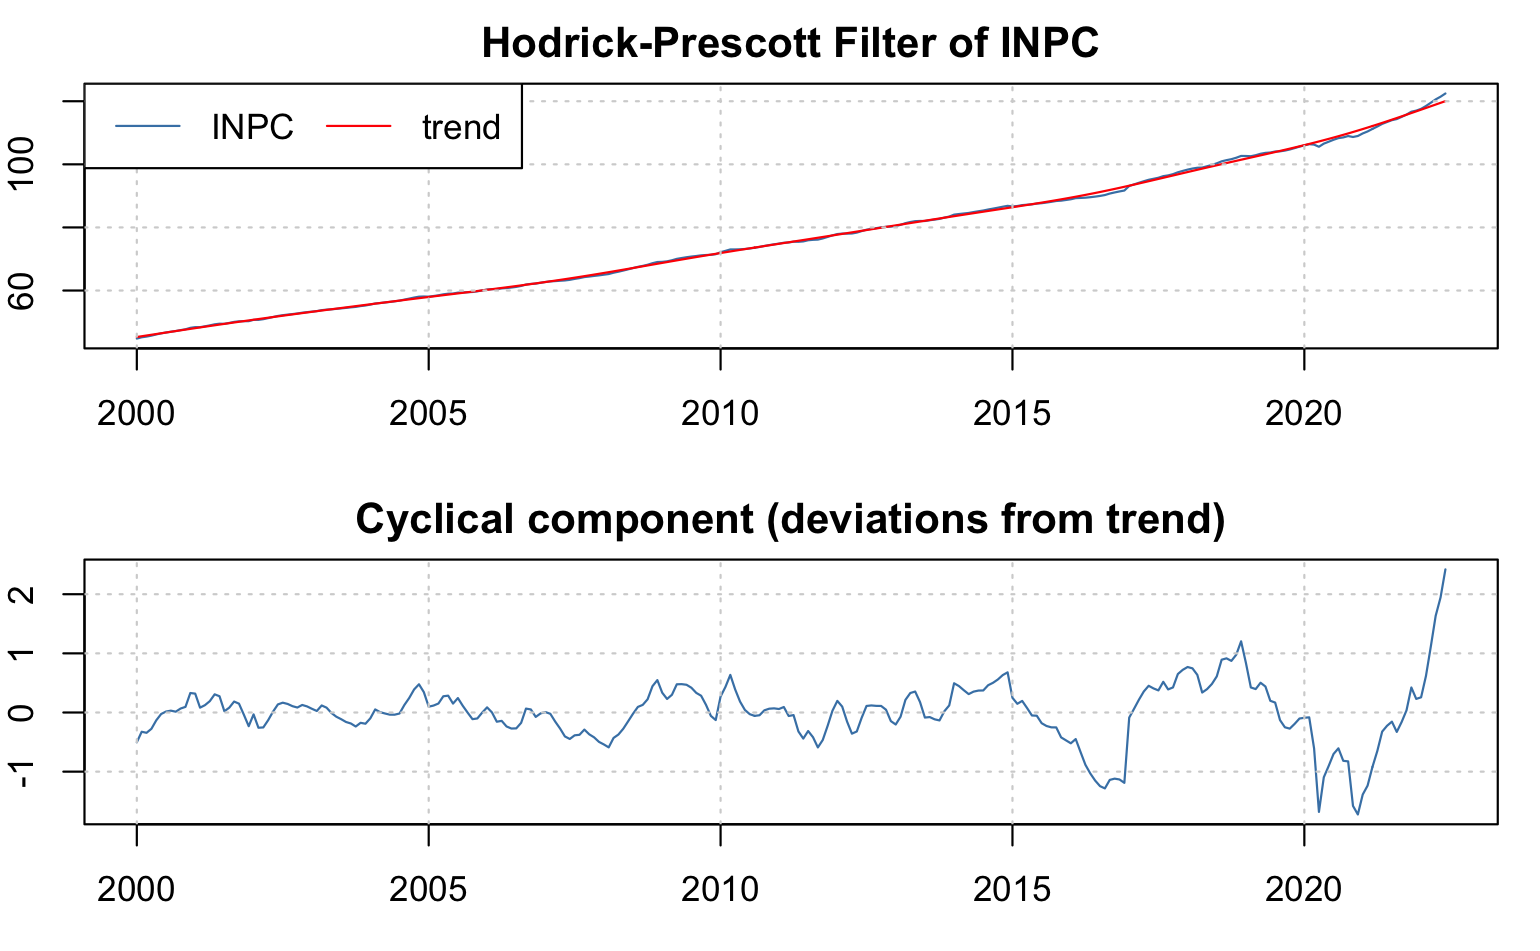
\includegraphics[width=0.95\linewidth]{Plots/G_INPC_HP} 

}

\caption{Descomposición del Índice Nacional de Precios al Consumidor ($INPC_t$) en su tendencia o trayectoria de largo plazo y su ciclo de corto plazo utilizando un filtro Hodrick y Prescott (1997)}\label{fig:fig52}
\end{figure}

\begin{Shaded}
\begin{Highlighting}[]
\NormalTok{TC\_hpf }\OtherTok{\textless{}{-}} \FunctionTok{hpfilter}\NormalTok{(TC, }\AttributeTok{freq =} \DecValTok{14400}\NormalTok{)}

\CommentTok{\#plot(TC\_hpf)}

\NormalTok{knitr}\SpecialCharTok{::}\FunctionTok{include\_graphics}\NormalTok{(}\StringTok{"Plots/G\_TC\_HP.png"}\NormalTok{) }
\end{Highlighting}
\end{Shaded}

\begin{figure}

{\centering 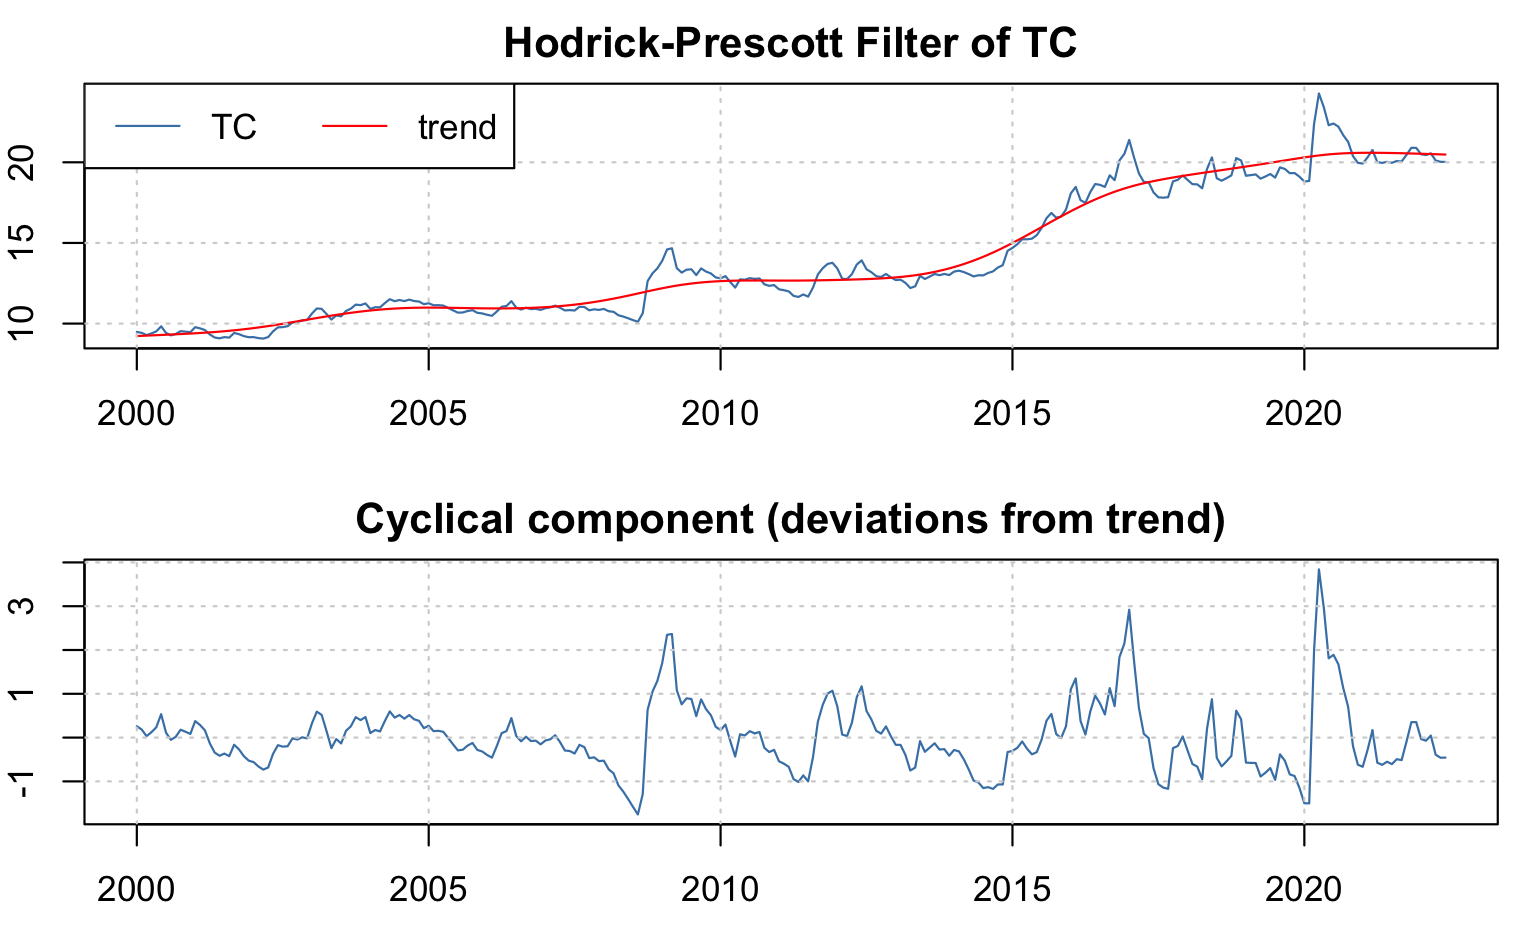
\includegraphics[width=0.95\linewidth]{Plots/G_TC_HP} 

}

\caption{Descomposición del Tipo de Cambio FIX ($TC_t$) en su tendencia o trayectoria de largo plazo y su ciclo de corto plazo utilizando un filtro Hodrick y Prescott (1997)}\label{fig:fig53}
\end{figure}

\hypertarget{filtro-hodrick-prescott-planteado-por-st-amant-van-norden}{%
\subsection{Filtro Hodrick-Prescott planteado por St-Amant \& van Norden}\label{filtro-hodrick-prescott-planteado-por-st-amant-van-norden}}

Existen una técnica adicional que soluciona un problema de distribuciones de colas pesadas es el planteado por St-Amant \& van Norden. Analicemos ese caso. Método tradicional de HP consiste en minimizar la serie \(\{ \tau_t \}_{t=-1}^T\):

\begin{equation}
  \sum_{t=1}^T (y_t - \tau_t)^2 + \lambda \sum_{t=1}^{T} [(\tau_{t} - \tau_{t-1}) - (\tau_{t-1} - \tau_{t-2})]^2
\end{equation}

Donde \(\lambda\) es un parámetro fijo (determinado ex-ante) y \(\tau_t\) es un componente de tendencia de \(y_t\).

Sin pérdida de generalidad, asumiremos que \(\tau_{-1}\) y \(\tau_{0}\) son cero (0). De esta manera, la forma matricial del filtro HP es:
\begin{equation}
  (Y - G)'(Y - G) + \lambda G' K' K G
\end{equation}

La derivada de los anteriores:
\begin{equation}
  -2 Y + 2 G + \lambda 2 K' K G = 0
\end{equation}

Despejando:
\begin{equation}
  G_{hp} = [I_T + \lambda K' K]^{-1} Y
\end{equation}

Donde \(G\) es el vector de tendencia, \(Y\) es el vector de la serie de datos, \(\lambda\) es la constante tradicional, y \(K\) es de dimensión \(T \times T\) y está dada por la expresión:
\begin{equation}
  K =
  \begin{pmatrix}
  1 & 0 & 0 & 0 & \ldots & 0 \\
  -2 & 1 & 0 & 0 & \ldots & 0 \\
  1 & -2 & 1 & 0 & \ldots & 0 \\
  0 & 1 & -2 & 1 & \ldots & 0 \\
  \vdots & \vdots &  \vdots &  \vdots &  \vdots &  \vdots \\
  0 & 0 & 0 & 0 & \ldots & 1 \\
  \end{pmatrix}
\end{equation}

Así:

\begin{equation}
  K' =
  \begin{pmatrix}
  1 & -2 & 1 & 0 & \ldots & 0 \\
  0 & 1 & -2 & 1 & \ldots & 0 \\
  0 & 0 & 1 & -2 & \ldots & 0 \\
  0 & 0 & 0 & 1 & \ldots & 0 \\
  \vdots & \vdots &  \vdots &  \vdots &  \vdots &  \vdots \\
  0 & 0 & 0 & 0 & \ldots & 1 \\
  \end{pmatrix}
\end{equation}

Método modificado de HP consiste en minimizar los valores de la serie \(\{ \tau_t \}_{t=1}^T\):
\begin{equation}
  \sum_{t=1}^T (y_t - \tau_t)^2 + \lambda \sum_{t=2}^{T-1} [(\tau_{t+1} - \tau_t) - (\tau_t     - \tau_{t-1})]^2 + \lambda_{ss} \sum_{t=T-j}^{T} [\Delta \tau_t - u_{ss}]
\end{equation}

Donde \(\lambda\) es una parámetro fijo (determinado ex-ante), \(\tau_t\) es un componente de tendencia de \(y_t\), y los nuevos parámetros son \(u_{ss}\) y \(\lambda_{ss}\) ajustadas por el procedimiento de Marcet y Ravn (2004).

Este procedimiento asume que parte del filtro HP y que esta versión tiene el problema de pérdida de información al final y al principio de la muestra. La razón es que es un procedimeinto univariado que requiere de mucha información futura y pasada para mejorar el ajuste.

El compoenente adicional al filtro HP es un componente de castigo por desviaciones de la tasa de crecimiento de largo plazo, \(u_{ss}\).

El proceso de selección de \(\lambda_{ss}\) es e propuesto por Marcet y Ravn (2004), el cual consiste en utilizar un \(\lambda\) convencional y el filtro HP convencional para estimar la siguiente función:
\begin{equation}
  F(\lambda) = \frac{\sum_{t=2}^{T-1} ((\tau_{t+1} - \tau_t) - (\tau_t -                 \tau_{t-1}))^2}{\sum_{t=1}^T (y_t - \tau_t)^2}
\end{equation}

Entonces el valor de \(\lambda_{ss}\) será aquel que:
\begin{equation}
  F(\lambda_{ss}) = \frac{\sum_{t=2}^{T-1} ((\tau_{t+1} - \tau_t) - (\tau_t - \tau_{t-1}))^2}{\sum_{t=1}^T (y_t - \tau_t)^2} = F(\lambda)
\end{equation}

Nota: Antón (2009) estimó \(\lambda_{ss} = 1096\) para datos trimestrales del PIB.

La forma matricial del filtro HP-SAVN es:
\begin{equation}
  (Y - G)'(Y - G) + \lambda G' K' K G + \lambda_{ss} (L^j G + \overline{u}_{ss} M^j)
\end{equation}

Donde \(L^j = (0, 0, \ldots, 0, -1, 0, \ldots, 0, 1)\), en el cual el valor \(-1\) es en la posición \(T-j-1\)-ésima, y \(M^j\) es un vector que toma valores de cero hasta antes de \(T-j\) y de 1 después.

La derivada de los anteriores:
\begin{equation}
  -2 Y + 2 G + \lambda 2 K' K G + \lambda_{ss} L'^j = 0
\end{equation}

Despejando:
\begin{equation}
  G_{SAVN} = \frac{1}{2} [I_T + \lambda K' K]^{-1} (2 Y - \lambda_{ss} L'^j)
\end{equation}

\begin{equation}
  G_{SAVN} = [I_T + \lambda K' K]^{-1} Y - \frac{1}{2} [I_T + \lambda K' K]^{-1} \lambda_{ss} L'^j
\end{equation}

Donde \(G\) es el vector de tendencia, \(Y\) es el vector de la serie de datos, \(\lambda\) es la constante tradicional, y \(K\) es de dimensión \(T \times T\) y está dada por la expresión:

\begin{equation}
  K' =
  \begin{pmatrix}
  1 & -2 & 1 & 0 & \ldots & 0 \\
  0 & 1 & -2 & 1 & \ldots & 0 \\
  \vdots & \vdots &  \vdots &  \vdots &  \vdots &  \vdots \\
  0 & 0 & 0 & 0 & \ldots & 1 \\
  \end{pmatrix}
\end{equation}

Dicho lo anterior, podemos modificar \(F(\lambda)\) para el filtro HP convencional como en forma matricial:
\begin{equation}
  F(\lambda) = \frac{G' K' K G}{(Y - G)'(Y - G)}
\end{equation}

\hypertarget{procesos-no-estacionarios-univariados}{%
\chapter{Procesos No Estacionarios Univariados}\label{procesos-no-estacionarios-univariados}}

\hypertarget{definiciuxf3n-y-formas-de-no-estacionariedad}{%
\section{Definición y formas de No Estacionariedad}\label{definiciuxf3n-y-formas-de-no-estacionariedad}}

Hasta ahora hemos planteado una serie de técnicas de regresión (AR, MA, ARMA, ARIMA, ARIMAX, etc.) que aplican sólo a procesos o series estacionarias. Sin embargo, no hemos proporcionado una prueba estadística para determinar si una serie es estacionaria. Ese es uno de los objetivos de esta sección.

Adicionalmente, en esta sección relajaremos la definición de estacionariedad y plantearemos pruebas para determinar cuándo una serie es estacionaria bajo tres diferentes especificaciones:

\begin{enumerate}
\def\labelenumi{\arabic{enumi}.}
\item
  Estacionariedad alrededor de una tendencia determinística;
\item
  Estacionariedad alrededor de una media, y
\item
  Estacionariedad alrededor del cero.
\end{enumerate}

A continuación, discutiremos cómo es posible que una serie sea estacionaria al rededor de una tendencia determinística. Diremos que una tendencia es determinística si ésta puede ser aproximada o modelada por un polinomio en función de \(t\), la cual incluye posibles transformaciones logarítmicas.

Bajo este enfoque, el proceso está lejos de cumplir con la definición de estacionariedad que hemos establecido en capítulos previos, pero relajaremos el supuesto y reconoceremos que una serie puede ser estacionaria en varianza bajo una tendencia determinística. Así, diremos que la serie será descrita por una ecuación dada por:
\begin{equation}
    Y_t = \sum^m_{j = 0} \delta_j t^j + X_t
    \label{eq:YTrend}
\end{equation}

Donde \(X_t\) es un proceso \(ARMA(p, q)\) con media cero, que se puede ver como:
\begin{equation}
    \alpha(L) X_t = \beta(L) U_t
\end{equation}

Entonces, los momentos y variaza de la ecuación \eqref{eq:YTrend} estarán dados por:
\begin{equation}
    \mathbb{E}[Y_t] = \sum^m_{j = 0} \delta_j t^j = \mu_t
    \label{eq:ETrend}
\end{equation}

Dada la ecuación \eqref{eq:ETrend} podemos plantear la siguiente ecuación de covarianzas:
\begin{eqnarray}
    \mathbb{E}[(Y_t - \mu_t) \cdot (Y_{t+\tau} - \mu_{t+\tau})] & = & \mathbb{E}[X_t \cdot X_{t+\tau}] \nonumber \\
    & = & \gamma_X(\tau)
    \label{eq:CovTrend}
\end{eqnarray}

Utilizando el resultado de la ecuación \eqref{eq:CovTrend} podemos establecer que:
\begin{equation}
    \mathbb{E}[(Y_t - \mu_t)^2] = \mathbb{E}[X_t^2] = \sigma_X^2
    \label{eq:VarTrend}
\end{equation}

Así, las ecuaciones \eqref{eq:ETrend} y \eqref{eq:VarTrend} significan que el proceso descrito por la ecuación \eqref{eq:YTrend} es estacionario pero en varianza. De esta forma, a partir de este momento diremos que una serie será estacionaria al rededor de una tendencia determinística si cumple con las condiciones establecidas en las ecuaciones \eqref{eq:YTrend}, \eqref{eq:ETrend} y \eqref{eq:VarTrend}.

Dicho lo anterior, estudiaremos el concepto de raíz unitaria de un proceso estocástico o de una serie de tiempo. Partamos de plantear que un proceso AR(1) tiene raíz unitaria cuando el coeficiente \(a_1 = 1\), es decir:
\begin{equation}
    Y_t = Y_{t-1} + U_t
    \label{eq:UR1}
\end{equation}

Donde \(U_t\) es un proceso puramente aleatorio con media cero, varianza constante y autocovarianza cero (0), al cual nos referiremos simplemente como ruido blanco. Supongamos ahora que incluimos un término constante en la ecuación \eqref{eq:UR1}, de forma que tenemos:
\begin{equation}
    Y_t = \delta + Y_{t-1} + U_t
    \label{eq:UR2}
\end{equation}

Tomando a la ecuación \eqref{eq:UR2} y suponiendo que existe un valor inicial \(Y_0\) de la serie, podemos plantear la siguiente secuencia de expresiones:
\begin{eqnarray*}
    Y_1 & = & \delta + Y_0 + U_1 \\
    Y_2 & = & \delta + Y_1 + U_2 \\
    & = & \delta + (\delta + Y_0 + U_1) + U_2 \\
    & = & 2 \times \delta + Y_0 + U_1 + U_2
\end{eqnarray*}

Si repitieramos la sustitución sucesiva anterior hasta el momento \(t\) encontrariamos que la ecuación de la solución general que describe a un \(AR(1)\) con término constante que tiene raíz unitaria es de la forma:
\begin{equation}
    Y_t = t \delta + Y_0 + \sum_{i=1}^t U_i
    \label{eq:UR3}
\end{equation}

La ecuación \eqref{eq:UR3} es equivalente a la ecuación \eqref{eq:YTrend}. A la ecuación \eqref{eq:UR3} también se le conoce como proceso con Drift o con término constante, indistintamente, ya que el componente de Drift suele asociarse a la posibilidad de incorporar el efecto de los residuales pasados, lo cual es posible simplemente agregando una constante.s

Si revisamos el comportamiento de sus momentos y varianza de la ecuación \eqref{eq:UR3} encontramos que:
\begin{eqnarray*}
    \mathbb{E}[Y_t] & = & Y_0 + \delta t = \mu_t \\
    Var[Y_t] & = & t \sigma^2 = \gamma(0, t) \\
    Cov(Y_t, Y_{t+\tau}) & = & (t - \tau) \sigma^2 = \gamma(t, \tau)
\end{eqnarray*}

De esta forma, la ecuación \eqref{eq:UR3} no describe un proceso estacionario, sólo podría ser estacionario si \(t = 1\), en cualquier otro caso sería no estacionario en varianza. Ahora hagamos un resumen y acordemos notación que se utilizará en esta sección. Supongamos un proceso o serie de tiempo que es descrito por la siguiente ecuación:
\begin{equation}
    Y_t = \delta + Y_{t-1} + X_t
    \label{eq:UR4}
\end{equation}

Donde \(X_t\) es un \(ARMA(p, q)\) con media cero. Si definimos a \(\Delta Y_t = Y_t - Y_{t-1}\), entonces la ecuación \eqref{eq:UR4} la podemos escribir como:
\begin{equation}
    \Delta Y_t = \delta + X_t
    \label{eq:UR5}
\end{equation}

A la ecuación \eqref{eq:UR5} la denominaremos como un proceso estacionario en diferencias o simplemente como un proceso integrado. Así, utilizaremos la siguiente definición.

Sea un proceso estocástico \(Y\), decimos que es un \textbf{proceso integrado de orden} \(d\), \(I(d)\), si este puede transformarse a uno estacionario, que sea invertible, mediante la diferenciación del mismo \(d\)-veces, es decir:
\begin{equation}
    (1 - L)^d Y_t = \delta + X_t
    \label{eq:UR6}
\end{equation}

Donde \(X_t\) es un proceso \(ARMA(p, q)\). De lo cual se infiere que en la ecuación \eqref{eq:UR6} \(Y_t\) será una \(ARIMA(p, d, q)\), el cual contiene \(d\) raíces unitarias. A estos procesos también se les conoce como procesos con tendencia estocástica.

Dada la discusión anterior, a continuación, plantearemos un resumen de cuáles son los dos casos a los cuales nos referiremos como procesos que no son estacionarios en media, pero que sí lo son en varianza. Estos casos son:
\begin{eqnarray}
    Y_t & = & Y_0 + \delta t + U_t \\
    Y_t & = & Y_0 + \delta + \sum_{i = 1}^t U_t
\end{eqnarray}

Ambos casos no son estacionarios en media, pero sí lo son en varianza. De ambos podemos decir que los choques o innovaciones del término de error tienen un efecto transitorio en el primero, pero permanentes en el segundo.

\hypertarget{pruebas-de-rauxedces-unitarias}{%
\section{Pruebas de Raíces Unitarias}\label{pruebas-de-rauxedces-unitarias}}

En esta sección plantearemos una serie de pruebas estadísticas para determinar cuándo una serie puede ser estacionaria bajo tres posibles casos:

\begin{enumerate}
\def\labelenumi{\arabic{enumi}.}
\item
  Estacionariedad alrededor de una tendencia determinística;
\item
  Estacionariedad alrededor de una media, y
\item
  Estacionariedad alrededor del cero.
\end{enumerate}

A continuación, mostraremos como ejemplo la aplicación de las pruebas de raíces unitarias a la serie de Tipo de Cambio en forma logarítmica y de diferencias logarítmicas. Asumamos que determinamos el valor de los rezagos de la prueba con el criterio de \(p = int\{ 4 (T/100)^{1/4} \}\). En la práctica, existen otras formas de determinar el valor de \(p\), como el criterio de AIC, pero es decisión del investigador cuál usar.

\begin{Shaded}
\begin{Highlighting}[]
\FunctionTok{library}\NormalTok{(ggplot2)}
\FunctionTok{library}\NormalTok{(dplyr)}
\FunctionTok{library}\NormalTok{(stats)}
\FunctionTok{library}\NormalTok{(MASS)}
\FunctionTok{library}\NormalTok{(strucchange)}
\FunctionTok{library}\NormalTok{(zoo)}
\FunctionTok{library}\NormalTok{(sandwich)}
\FunctionTok{library}\NormalTok{(urca)}
\FunctionTok{library}\NormalTok{(lmtest)}
\FunctionTok{library}\NormalTok{(vars)}

\CommentTok{\#}
\FunctionTok{load}\NormalTok{(}\StringTok{"BD/Datos\_Ad.RData"}\NormalTok{)}

\CommentTok{\#}
\DocumentationTok{\#\# Conversion a series de tiempo:}
\NormalTok{Datos }\OtherTok{\textless{}{-}} \FunctionTok{ts}\NormalTok{(Datos\_Ad[}\DecValTok{7}\SpecialCharTok{:} \DecValTok{11}\NormalTok{], }
            \AttributeTok{start =} \FunctionTok{c}\NormalTok{(}\DecValTok{2000}\NormalTok{, }\DecValTok{1}\NormalTok{), }
            \AttributeTok{freq =} \DecValTok{12}\NormalTok{)}

\NormalTok{LDatos }\OtherTok{\textless{}{-}} \FunctionTok{log}\NormalTok{(Datos)}

\NormalTok{DLDatos }\OtherTok{\textless{}{-}} \FunctionTok{diff}\NormalTok{(}\FunctionTok{log}\NormalTok{(Datos, }\AttributeTok{base =} \FunctionTok{exp}\NormalTok{(}\DecValTok{1}\NormalTok{)), }
                \AttributeTok{lag =} \DecValTok{1}\NormalTok{, }
                \AttributeTok{differences =} \DecValTok{1}\NormalTok{)}

\NormalTok{DaLDatos }\OtherTok{\textless{}{-}} \FunctionTok{diff}\NormalTok{(}\FunctionTok{log}\NormalTok{(Datos, }\AttributeTok{base =} \FunctionTok{exp}\NormalTok{(}\DecValTok{1}\NormalTok{)), }
                 \AttributeTok{lag =} \DecValTok{12}\NormalTok{, }
                 \AttributeTok{differences =} \DecValTok{1}\NormalTok{)}
\end{Highlighting}
\end{Shaded}

Como primer paso, exploraremos las series en niveles (bajo una transformación logarítmica), como en la Figura \ref{fig:fig71}, y en diferencias logarítmicas, como en la Figura \ref{fig:fig72}. De dicha exploración, podemos concluir que las series parecen estacionarias en diferencias, pero no en niveles.

\begin{Shaded}
\begin{Highlighting}[]
\FunctionTok{plot}\NormalTok{(LDatos, }
     \AttributeTok{plot.type =} \StringTok{"m"}\NormalTok{, }\AttributeTok{nc =} \DecValTok{2}\NormalTok{,}
     \AttributeTok{col =} \FunctionTok{c}\NormalTok{(}\StringTok{"darkgreen"}\NormalTok{, }\StringTok{"darkblue"}\NormalTok{, }\StringTok{"darkred"}\NormalTok{, }\StringTok{"orange"}\NormalTok{, }\StringTok{"purple"}\NormalTok{), }
     \AttributeTok{main =} \StringTok{"Series en Logaritmos"}\NormalTok{, }
     \AttributeTok{xlab =} \StringTok{"Tiempo"}\NormalTok{)}
\end{Highlighting}
\end{Shaded}

\begin{figure}

{\centering 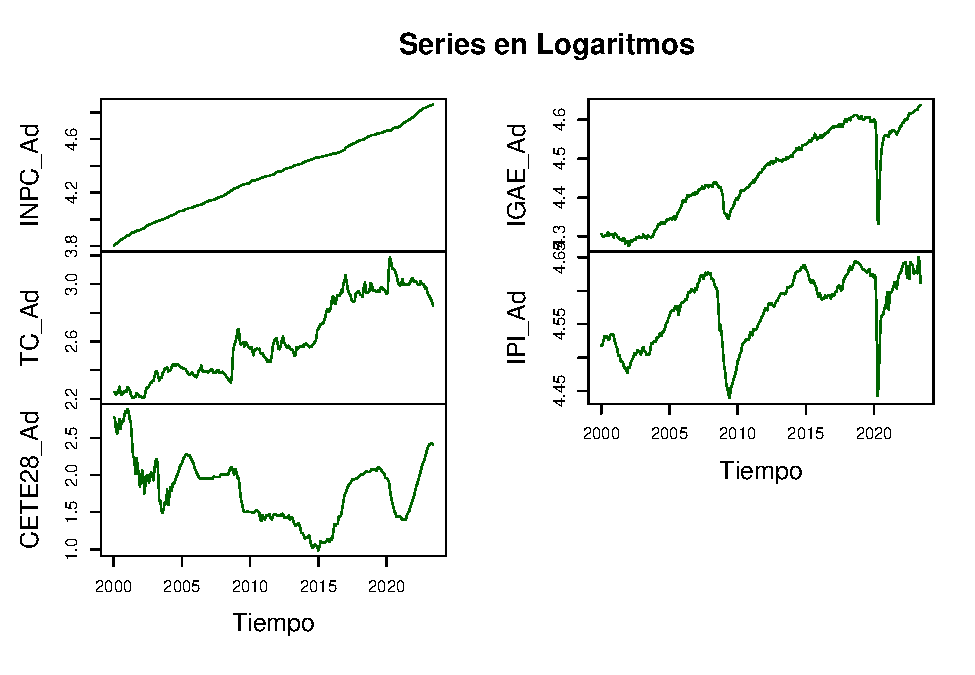
\includegraphics{Notas-Series-Tiempo_files/figure-latex/fig71-1} 

}

\caption{Series en Logaritmos}\label{fig:fig71}
\end{figure}

\begin{Shaded}
\begin{Highlighting}[]
\FunctionTok{plot}\NormalTok{(DLDatos, }
     \AttributeTok{plot.type =} \StringTok{"m"}\NormalTok{, }\AttributeTok{nc =} \DecValTok{2}\NormalTok{,}
     \AttributeTok{col =} \FunctionTok{c}\NormalTok{(}\StringTok{"darkgreen"}\NormalTok{, }\StringTok{"darkblue"}\NormalTok{, }\StringTok{"darkred"}\NormalTok{, }\StringTok{"orange"}\NormalTok{, }\StringTok{"purple"}\NormalTok{), }
     \AttributeTok{main =} \StringTok{"Series en Diferencias Logaritmicas"}\NormalTok{, }
     \AttributeTok{xlab =} \StringTok{"Tiempo"}\NormalTok{)}
\end{Highlighting}
\end{Shaded}

\begin{figure}

{\centering 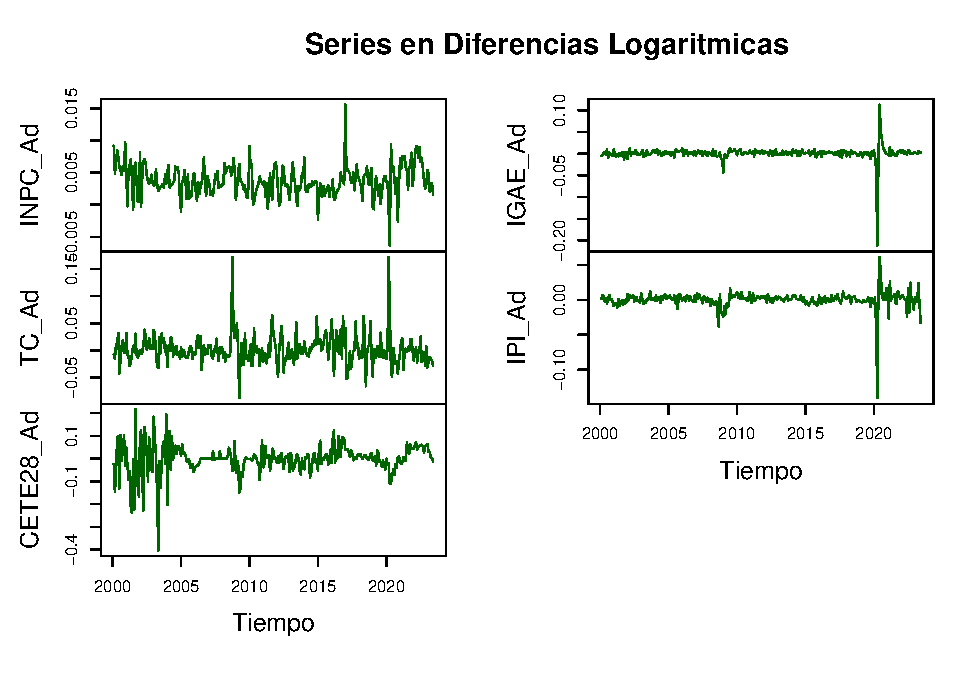
\includegraphics{Notas-Series-Tiempo_files/figure-latex/fig72-1} 

}

\caption{Series en Diferencias Logaritmicas}\label{fig:fig72}
\end{figure}

\begin{Shaded}
\begin{Highlighting}[]
\FunctionTok{plot}\NormalTok{(DaLDatos, }
     \AttributeTok{plot.type =} \StringTok{"m"}\NormalTok{, }\AttributeTok{nc =} \DecValTok{2}\NormalTok{,}
     \AttributeTok{col =} \FunctionTok{c}\NormalTok{(}\StringTok{"darkgreen"}\NormalTok{, }\StringTok{"darkblue"}\NormalTok{, }\StringTok{"darkred"}\NormalTok{, }\StringTok{"orange"}\NormalTok{, }\StringTok{"purple"}\NormalTok{), }
     \AttributeTok{main =} \StringTok{"Series en Diferencias Anuales Logaritmicas"}\NormalTok{, }
     \AttributeTok{xlab =} \StringTok{"Tiempo"}\NormalTok{)}
\end{Highlighting}
\end{Shaded}

\begin{figure}

{\centering 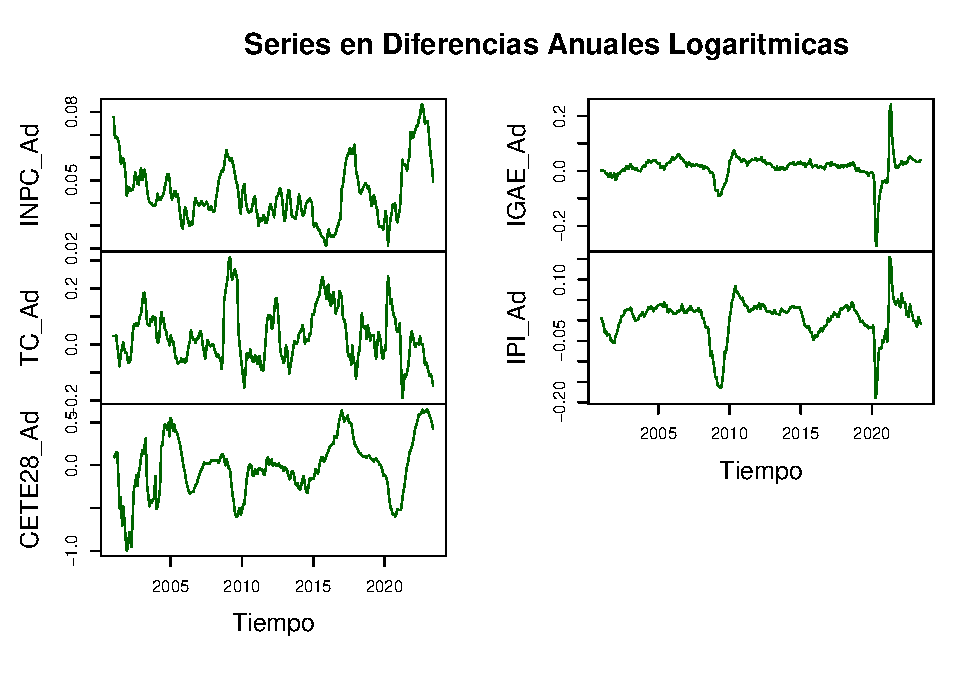
\includegraphics{Notas-Series-Tiempo_files/figure-latex/fig73-1} 

}

\caption{Series en Diferencias Anuales Logaritmicas}\label{fig:fig73}
\end{figure}

\begin{Shaded}
\begin{Highlighting}[]
\FunctionTok{plot}\NormalTok{(}\FunctionTok{cbind}\NormalTok{(DLDatos, DaLDatos), }
     \AttributeTok{plot.type =} \StringTok{"m"}\NormalTok{, }\AttributeTok{nc =} \DecValTok{2}\NormalTok{,}
     \AttributeTok{col =} \FunctionTok{c}\NormalTok{(}\StringTok{"darkgreen"}\NormalTok{, }\StringTok{"darkblue"}\NormalTok{, }\StringTok{"darkred"}\NormalTok{, }\StringTok{"orange"}\NormalTok{, }\StringTok{"purple"}\NormalTok{), }
     \AttributeTok{main =} \StringTok{"Comparacion de Series en Diferencias"}\NormalTok{, }
     \AttributeTok{xlab =} \StringTok{"Tiempo"}\NormalTok{)}
\end{Highlighting}
\end{Shaded}

\begin{figure}

{\centering 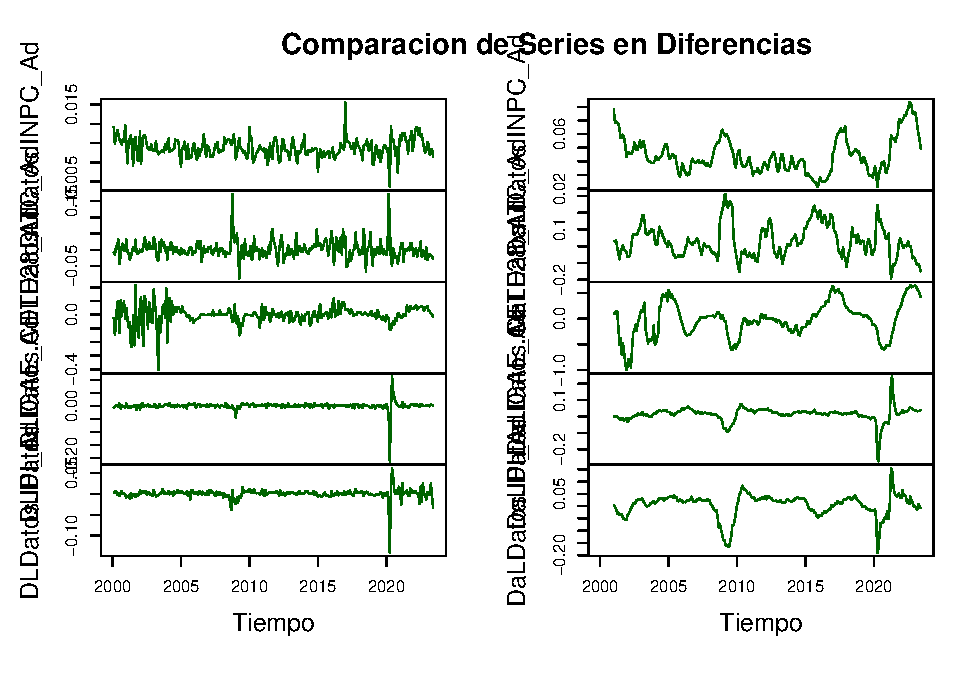
\includegraphics{Notas-Series-Tiempo_files/figure-latex/fig74-1} 

}

\caption{Comparacion de Series en Diferencias Anuales}\label{fig:fig74}
\end{figure}

\begin{Shaded}
\begin{Highlighting}[]
\FunctionTok{plot}\NormalTok{(}\FunctionTok{cbind}\NormalTok{(LDatos, DLDatos), }
     \AttributeTok{plot.type =} \StringTok{"m"}\NormalTok{, }\AttributeTok{nc =} \DecValTok{2}\NormalTok{,}
     \AttributeTok{col =} \FunctionTok{c}\NormalTok{(}\StringTok{"darkgreen"}\NormalTok{, }\StringTok{"darkblue"}\NormalTok{, }\StringTok{"darkred"}\NormalTok{, }\StringTok{"orange"}\NormalTok{, }\StringTok{"purple"}\NormalTok{), }
     \AttributeTok{main =} \StringTok{"Comparacion de Series en Diferencias"}\NormalTok{, }
     \AttributeTok{xlab =} \StringTok{"Tiempo"}\NormalTok{)}
\end{Highlighting}
\end{Shaded}

\begin{figure}

{\centering 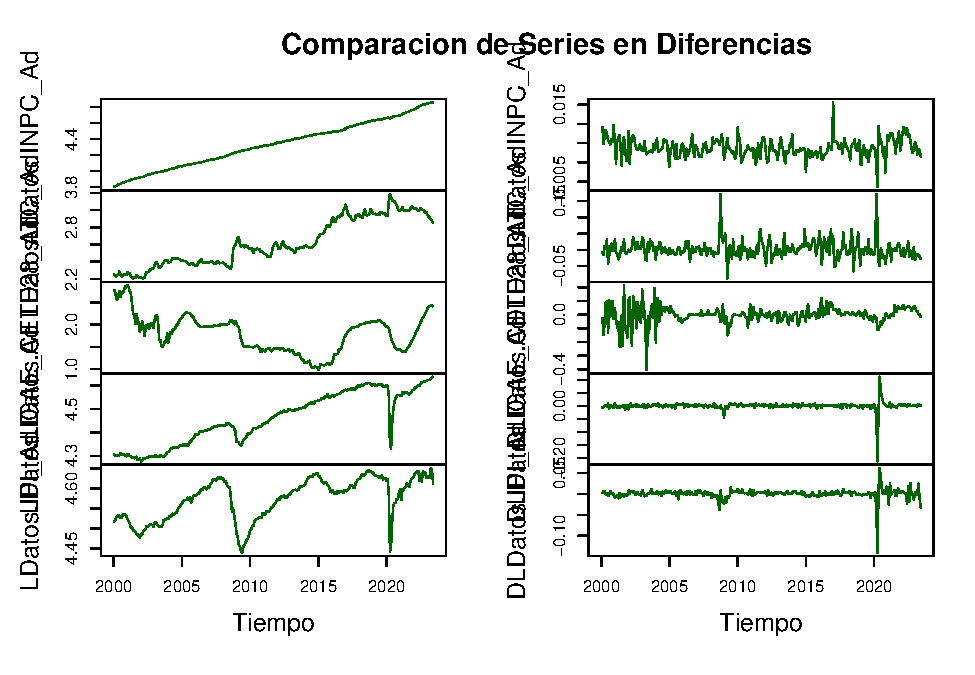
\includegraphics{Notas-Series-Tiempo_files/figure-latex/fig75-1} 

}

\caption{Comparacion de Series en Diferencias}\label{fig:fig75}
\end{figure}

\hypertarget{dickey---fuller-df}{%
\subsection{Dickey - Fuller (DF)}\label{dickey---fuller-df}}

Partamos de una forma del proceso \(Y_t\) dada por:
\begin{equation}
    Y_t = \sum_{j = 0}^m \delta_j t^j + X_t
    \label{eq:URDFG}
\end{equation}

Donde \(X_t\) es un \(ARMA(p, q)\) con media cero. Esta prueba asume que \(m = 1\), por lo que utilizaremos un modelo del tipo:
\begin{equation}
    Y_t = \alpha + \delta t + \rho Y_{t-1} + U_t
    \label{eq:URDF}
\end{equation}

Si, el \(AR(1)\) planteado tiene raíz unitaria, es decir, \(\rho = 1\), entonces tendríamos:
\begin{eqnarray*}
    Y_t & = & \alpha + \delta t + Y_{t-1} + U_t \\
    \Delta Y_t & = & \alpha + \delta t + U_t
\end{eqnarray*}

De esta forma, para determinar si una serie tiene raíz unitaria basta con probar la hipótesis nula de que \(H_0 : \rho = 1\), junto con las diferentes combinaciones que impliquen restricciones respecto a \(\delta\) y \(\alpha\).

En resumen, la prueba DF consiste en asumir un modelo general dado por la ecuación \eqref{eq:URDF} y probar tres especificaciones distintas que serían válidas bajo \(H_0 : \rho = 1\):

\begin{enumerate}
\def\labelenumi{\arabic{enumi}.}
\item
  Modelo A: con intercepto y tendencia:
  \begin{equation*}
   \Delta Y_t = \alpha + \delta t + \beta Y_{t-1} + U_t
    \end{equation*}
  Buscamos probar si \(H_0 : \beta = \rho - 1 = 0\) contra \(H_a : \beta < 0\), por lo que es una prueba de una cola. Otra forma de decirlo es: probamos si el proceso tiene raíz unitaria contra si el proceso es estacionario alrededor de una tendencia determinística.
\item
  Modelo B: con intercepto:
  \begin{equation*}
   \Delta Y_t = \alpha + \beta Y_{t-1} + U_t
    \end{equation*}
  Buscamos probar si \(H_0 : \beta = \rho - 1 = 0\) contra \(H_a : \beta < 0\), por lo que es una prueba de una cola. Otra forma de decirlo es: probamos si el proceso tiene raíz unitaria contra si el proceso es estacionario alrededor de una constante.
\item
  Modelo C: sin intercepto y tendencia:
  \begin{equation*}
   \Delta Y_t = \beta Y_{t-1} + U_t
    \end{equation*}
  Buscamos probar si \(H_0 : \beta = \rho - 1 = 0\) contra \(H_a : \beta < 0\), por lo que es una prueba de una cola. Otra forma de decirlo es: probamos si el proceso tiene raíz unitaria contra si el proceso es estacionario sin considerar una constante o una tendencia determinística, es decir, es un proceso puramente aleatorio.
\end{enumerate}

\textbf{Ejemplo}. En los siguientes mostramos los resultados de aplicar las pruebas de raíces unitarias a la serie \(LTC_t\), considerando \(p = int \{ 4 (234/100)^{(1/4)} \} = 4\) para aquellas pruebas que requieren de rezagos: ADF, PP y KPSS. La convención es implementar las pruebas de raíces unitarias iniciando con el modelo más general hasta llegar al más restringido. Es decir, iniciar con el Modelo A, pasar al Modelo B y cerrar con el Modelo C.

Iniciaremos implementando una prueba de DF simple (o una ADF sin rezagos). En este caso obtenemos los resultados mostrados en la siguiente Tabla. En esta se reportan los resultados de la prueba para cada uno de los 3 modelos (A, B y C) y los valores críticos (CV, por sus siglas en inglés) de la prueba para los niveles 1\%, 5\% y 10\%--estos valores son los reportados por MacKinnon (1996) para una prueba con distribución de 1 cola (izquierda). La convención es utilizar el nivel del 5\% de significancia.

Los resultados deben leerse de la siguiente forma. La siguiente Tabla muestra los resultados de la prueba para la serie en niveles, \(LTC_t\), y en diferencias \(\Delta LTC_t\). De esta forma, podremos comparar si la serie es estacionaria en niveles o en diferencias. La manera de determinarlo es comparar el estadístico con el valor crítico. Así, rechazaremos la hipótesis nula en los casos en que el estadístico \(t\) se ubique por encima del valor crítico. En este caso, podemos observar que la serie se vuelve estacionaria hasta su primera diferencia--caso en el que rechazamos la hipótesis nula en todos los modelos.

\begin{longtable}[]{@{}llccc@{}}
\caption{\label{tab:DF-summary} Resumen de resultados de la prueba Dickey-Fuller (DF).}\tabularnewline
\toprule\noalign{}
\textbf{Model} & \textbf{Estadístico} & \textbf{1\% CV} & \textbf{5\% CV} & \textbf{10\% CV} \\
\midrule\noalign{}
\endfirsthead
\toprule\noalign{}
\textbf{Model} & \textbf{Estadístico} & \textbf{1\% CV} & \textbf{5\% CV} & \textbf{10\% CV} \\
\midrule\noalign{}
\endhead
\bottomrule\noalign{}
\endlastfoot
\textbf{LTC\_t} & & & & \\
Modelo A & \(t=-2.0752\) & \(-3.98\) & \(-3.42\) & \(-3.13\) \\
Modelo B & \(t=-1.1724\) & \(-3.44\) & \(-2.87\) & \(-2.57\) \\
Modelo C & \(t=1.1815\) & \(-2.58\) & \(-1.95\) & \(-1.62\) \\
\textbf{\(\Delta LTC_t\)} & & & & \\
Modelo A & \(t=-12.6805\) & \(-3.98\) & \(-3.42\) & \(-3.13\) \\
Modelo B & \(t=-12.6899\) & \(-3.44\) & \(-2.87\) & \(-2.57\) \\
Modelo C & \(t=-12.6515\) & \(-2.58\) & \(-1.95\) & \(-1.62\) \\
\end{longtable}

\begin{Shaded}
\begin{Highlighting}[]
\DocumentationTok{\#\# Dickey{-}Fuller:}

\DocumentationTok{\#\#\# NIVELES: Tipo de cambio}

\FunctionTok{summary}\NormalTok{(}\FunctionTok{ur.df}\NormalTok{(LDatos[, }\DecValTok{2}\NormalTok{], }\AttributeTok{type =} \StringTok{"trend"}\NormalTok{, }\AttributeTok{lags =} \DecValTok{0}\NormalTok{))}
\end{Highlighting}
\end{Shaded}

\begin{verbatim}
## 
## ############################################### 
## # Augmented Dickey-Fuller Test Unit Root Test # 
## ############################################### 
## 
## Test regression trend 
## 
## 
## Call:
## lm(formula = z.diff ~ z.lag.1 + 1 + tt)
## 
## Residuals:
##       Min        1Q    Median        3Q       Max 
## -0.083973 -0.015415 -0.002526  0.009332  0.170645 
## 
## Coefficients:
##                Estimate  Std. Error t value Pr(>|t|)  
## (Intercept)  0.08700923  0.04029878   2.159   0.0317 *
## z.lag.1     -0.03844435  0.01852595  -2.075   0.0389 *
## tt           0.00011203  0.00006246   1.794   0.0740 .
## ---
## Signif. codes:  0 '***' 0.001 '**' 0.01 '*' 0.05 '.' 0.1 ' ' 1
## 
## Residual standard error: 0.02705 on 278 degrees of freedom
## Multiple R-squared:  0.01629,    Adjusted R-squared:  0.00921 
## F-statistic: 2.301 on 2 and 278 DF,  p-value: 0.102
## 
## 
## Value of test-statistic is: -2.0752 2.1124 2.3013 
## 
## Critical values for test statistics: 
##       1pct  5pct 10pct
## tau3 -3.98 -3.42 -3.13
## phi2  6.15  4.71  4.05
## phi3  8.34  6.30  5.36
\end{verbatim}

\begin{Shaded}
\begin{Highlighting}[]
\FunctionTok{summary}\NormalTok{(}\FunctionTok{ur.df}\NormalTok{(LDatos[, }\DecValTok{2}\NormalTok{], }\AttributeTok{type =} \StringTok{"drift"}\NormalTok{, }\AttributeTok{lags =} \DecValTok{0}\NormalTok{))}
\end{Highlighting}
\end{Shaded}

\begin{verbatim}
## 
## ############################################### 
## # Augmented Dickey-Fuller Test Unit Root Test # 
## ############################################### 
## 
## Test regression drift 
## 
## 
## Call:
## lm(formula = z.diff ~ z.lag.1 + 1)
## 
## Residuals:
##       Min        1Q    Median        3Q       Max 
## -0.089442 -0.014571 -0.002497  0.009620  0.171964 
## 
## Coefficients:
##              Estimate Std. Error t value Pr(>|t|)
## (Intercept)  0.020316   0.015600   1.302    0.194
## z.lag.1     -0.006946   0.005925  -1.172    0.242
## 
## Residual standard error: 0.02716 on 279 degrees of freedom
## Multiple R-squared:  0.004903,   Adjusted R-squared:  0.001336 
## F-statistic: 1.375 on 1 and 279 DF,  p-value: 0.242
## 
## 
## Value of test-statistic is: -1.1724 1.5477 
## 
## Critical values for test statistics: 
##       1pct  5pct 10pct
## tau2 -3.44 -2.87 -2.57
## phi1  6.47  4.61  3.79
\end{verbatim}

\begin{Shaded}
\begin{Highlighting}[]
\FunctionTok{summary}\NormalTok{(}\FunctionTok{ur.df}\NormalTok{(LDatos[, }\DecValTok{2}\NormalTok{], }\AttributeTok{type =} \StringTok{"none"}\NormalTok{, }\AttributeTok{lags =} \DecValTok{0}\NormalTok{))}
\end{Highlighting}
\end{Shaded}

\begin{verbatim}
## 
## ############################################### 
## # Augmented Dickey-Fuller Test Unit Root Test # 
## ############################################### 
## 
## Test regression none 
## 
## 
## Call:
## lm(formula = z.diff ~ z.lag.1 - 1)
## 
## Residuals:
##       Min        1Q    Median        3Q       Max 
## -0.089736 -0.014701 -0.003293  0.010359  0.169748 
## 
## Coefficients:
##          Estimate Std. Error t value Pr(>|t|)
## z.lag.1 0.0007280  0.0006161   1.181    0.238
## 
## Residual standard error: 0.0272 on 280 degrees of freedom
## Multiple R-squared:  0.004961,   Adjusted R-squared:  0.001407 
## F-statistic: 1.396 on 1 and 280 DF,  p-value: 0.2384
## 
## 
## Value of test-statistic is: 1.1815 
## 
## Critical values for test statistics: 
##       1pct  5pct 10pct
## tau1 -2.58 -1.95 -1.62
\end{verbatim}

\begin{Shaded}
\begin{Highlighting}[]
\DocumentationTok{\#\#\# DIFERENCIAS: Tipo de cambio}

\FunctionTok{summary}\NormalTok{(}\FunctionTok{ur.df}\NormalTok{(DLDatos[, }\DecValTok{2}\NormalTok{], }\AttributeTok{type =} \StringTok{"trend"}\NormalTok{, }\AttributeTok{lags =} \DecValTok{0}\NormalTok{))}
\end{Highlighting}
\end{Shaded}

\begin{verbatim}
## 
## ############################################### 
## # Augmented Dickey-Fuller Test Unit Root Test # 
## ############################################### 
## 
## Test regression trend 
## 
## 
## Call:
## lm(formula = z.diff ~ z.lag.1 + 1 + tt)
## 
## Residuals:
##      Min       1Q   Median       3Q      Max 
## -0.09095 -0.01306 -0.00158  0.01055  0.17069 
## 
## Coefficients:
##                 Estimate   Std. Error t value            Pr(>|t|)    
## (Intercept)  0.002881589  0.003163345   0.911               0.363    
## z.lag.1     -0.736373275  0.058071315 -12.680 <0.0000000000000002 ***
## tt          -0.000009351  0.000019483  -0.480               0.632    
## ---
## Signif. codes:  0 '***' 0.001 '**' 0.01 '*' 0.05 '.' 0.1 ' ' 1
## 
## Residual standard error: 0.02634 on 277 degrees of freedom
## Multiple R-squared:  0.3673, Adjusted R-squared:  0.3628 
## F-statistic: 80.41 on 2 and 277 DF,  p-value: < 0.00000000000000022
## 
## 
## Value of test-statistic is: -12.6805 53.6071 80.4095 
## 
## Critical values for test statistics: 
##       1pct  5pct 10pct
## tau3 -3.98 -3.42 -3.13
## phi2  6.15  4.71  4.05
## phi3  8.34  6.30  5.36
\end{verbatim}

\begin{Shaded}
\begin{Highlighting}[]
\FunctionTok{summary}\NormalTok{(}\FunctionTok{ur.df}\NormalTok{(DLDatos[, }\DecValTok{2}\NormalTok{], }\AttributeTok{type =} \StringTok{"drift"}\NormalTok{, }\AttributeTok{lags =} \DecValTok{0}\NormalTok{))}
\end{Highlighting}
\end{Shaded}

\begin{verbatim}
## 
## ############################################### 
## # Augmented Dickey-Fuller Test Unit Root Test # 
## ############################################### 
## 
## Test regression drift 
## 
## 
## Call:
## lm(formula = z.diff ~ z.lag.1 + 1)
## 
## Residuals:
##       Min        1Q    Median        3Q       Max 
## -0.090664 -0.013492 -0.001331  0.010702  0.169754 
## 
## Coefficients:
##              Estimate Std. Error t value            Pr(>|t|)    
## (Intercept)  0.001566   0.001577   0.993               0.322    
## z.lag.1     -0.735658   0.057972 -12.690 <0.0000000000000002 ***
## ---
## Signif. codes:  0 '***' 0.001 '**' 0.01 '*' 0.05 '.' 0.1 ' ' 1
## 
## Residual standard error: 0.02631 on 278 degrees of freedom
## Multiple R-squared:  0.3668, Adjusted R-squared:  0.3645 
## F-statistic:   161 on 1 and 278 DF,  p-value: < 0.00000000000000022
## 
## 
## Value of test-statistic is: -12.6899 80.5185 
## 
## Critical values for test statistics: 
##       1pct  5pct 10pct
## tau2 -3.44 -2.87 -2.57
## phi1  6.47  4.61  3.79
\end{verbatim}

\begin{Shaded}
\begin{Highlighting}[]
\FunctionTok{summary}\NormalTok{(}\FunctionTok{ur.df}\NormalTok{(DLDatos[, }\DecValTok{2}\NormalTok{], }\AttributeTok{type =} \StringTok{"none"}\NormalTok{, }\AttributeTok{lags =} \DecValTok{0}\NormalTok{))}
\end{Highlighting}
\end{Shaded}

\begin{verbatim}
## 
## ############################################### 
## # Augmented Dickey-Fuller Test Unit Root Test # 
## ############################################### 
## 
## Test regression none 
## 
## 
## Call:
## lm(formula = z.diff ~ z.lag.1 - 1)
## 
## Residuals:
##       Min        1Q    Median        3Q       Max 
## -0.089121 -0.011916  0.000311  0.012192  0.171310 
## 
## Coefficients:
##         Estimate Std. Error t value            Pr(>|t|)    
## z.lag.1 -0.73093    0.05777  -12.65 <0.0000000000000002 ***
## ---
## Signif. codes:  0 '***' 0.001 '**' 0.01 '*' 0.05 '.' 0.1 ' ' 1
## 
## Residual standard error: 0.02631 on 279 degrees of freedom
## Multiple R-squared:  0.3646, Adjusted R-squared:  0.3623 
## F-statistic: 160.1 on 1 and 279 DF,  p-value: < 0.00000000000000022
## 
## 
## Value of test-statistic is: -12.6515 
## 
## Critical values for test statistics: 
##       1pct  5pct 10pct
## tau1 -2.58 -1.95 -1.62
\end{verbatim}

\hypertarget{dickey---fuller-aumentada-adf}{%
\subsection{Dickey - Fuller Aumentada (ADF)}\label{dickey---fuller-aumentada-adf}}

A diferencia de un modelo AR(1) para el caso de una prueba DF como en la ecuación \eqref{eq:URDF}, en una prueba ADF se asume que el proceso es un AR(p) de la forma (por simplicidad, hemos omitido el término constante y el término de tendencia determinística):
\begin{equation}
    Y_t = a_1 Y_{t-1} + a_2 Y_{t-2} + \ldots + a_p Y_{t-p} + U_t
    \label{eq:URADF}
\end{equation}

Haciendo una sustitución de términos similar a las que hemos planteado en otras secciones, podemos reexpresar la ecuación \eqref{eq:URADF} en su versión en diferencias siguiendo el proceso:
\begin{equation}
    Y_t = \rho Y_{t-1} + \theta_1 \Delta Y_{t-1} + \theta_2 \Delta Y_{t-2} + \ldots + + \theta_{p-1} \Delta Y_{t-p+1} + U_t 
\end{equation}

Donde \(\rho = \theta_0 = \sum_{j = 1}^p a_j\), \(\theta_i = - \sum_{j = i + 1}^p a_j\), \(i = 1, 2, \ldots, p-1\). Así, si el proceso AR(p) tiene raíz unitaria, entonces, veremos que:
\begin{eqnarray*}
    1 - a_1 - a_2 - \ldots - a_p & = & 0 \\
    \rho & = & 1
\end{eqnarray*}

De donde podemos establecer que el modelo general de una prueba ADF será:
\begin{equation}
    \Delta Y_{t-1} = \alpha + \beta t + (\rho - 1) Y_{t-1} + \theta_1 \Delta Y_{t-1} + \theta_2 \Delta Y_{t-2} + \ldots + \theta_k \Delta Y_{t-k} + U_t
\end{equation}

Donde \(U_t\) es un proceso puramente aleatorio y \(k\) es elegido de tal manera que los residuales sean un proceso puramente aleatorio. En resumen, la prueba ADF consiste en asumir un modelo general dado por la ecuación \eqref{eq:URADF}, que incluya constante y tendencia, y probar tres especificaciones distintas que serían válidas bajo \(H_0 : \rho = 1\):

\begin{enumerate}
\def\labelenumi{\arabic{enumi}.}
\item
  Modelo A: con intercepto y tendencia:
  \begin{equation*}
  \Delta Y_t = \alpha + \delta t + \beta Y_{t-1} + \theta_1 \Delta Y_{t-1} + \theta_2 \Delta Y_{t-2} + \ldots + \theta_{p-1} \Delta Y_{t-p+1} + U_t
    \end{equation*}
  Buscamos probar si \(H_0 : \beta = \rho - 1 = 0\) contra \(H_a : \beta < 0\), por lo que es una prueba de una cola. Otra forma de decirlo es: probamos si el proceso tiene raíz unitaria contra si el proceso es estacionario alrededor de una tendencia determinística.
\item
  Modelo B: con intercepto:
  \begin{equation*}
   \Delta Y_t = \alpha + \beta Y_{t-1} + \theta_1 \Delta Y_{t-1} + \theta_2 \Delta Y_{t-2} + \ldots + \theta_{p-1} \Delta Y_{t-p+1} + U_t
    \end{equation*}
  Buscamos probar si \(H_0 : \beta = \rho - 1 = 0\) contra \(H_a : \beta < 0\), por lo que es una prueba de una cola. Otra forma de decirlo es: probamos si el proceso tiene raíz unitaria contra si el proceso es estacionario alrededor de una constante.
\item
  Modelo C: sin intercepto y tendencia:
  \begin{equation*}
   \Delta Y_t = \beta Y_{t-1} + \theta_1 \Delta Y_{t-1} + \theta_2 \Delta Y_{t-2} + \ldots + \theta_{p-1} \Delta Y_{t-p+1} + U_t
    \end{equation*}
  Buscamos probar si \(H_0 : \beta = \rho - 1 = 0\) contra \(H_a : \beta < 0\), por lo que es una prueba de una cola. Otra forma de decirlo es: probamos si el proceso tiene raíz unitaria contra si el proceso es estacionario sin considerar una constante o una tendencia determinística, es decir, es un proceso puramente aleatorio.
\end{enumerate}

\textbf{Ejemplo}. La siguiente Tabla muestra los resultados de la prueba para la serie en niveles, \(LTC_t\), y en diferencias \(\Delta LTC_t\) de una prueba ADF. De esta forma, podremos comparar si la serie es estacionaria en niveles o en diferencias. La manera de determinarlo es, al igual que en el caso anterior, comparar el estadístico con el valor crítico. Así, rechazaremos la hipótesis nula en los casos en que el estadístico \(t\) se ubique por encima del valor crítico. En este caso, podemos observar que la serie se vuelve estacionaria hasta su primera diferencia--caso en el que rechazamos la hipótesis nula en todos los modelos.

\begin{longtable}[]{@{}llccc@{}}
\caption{\label{tab:DF-summary} Resumen de resultados de la prueba Augmented Dickey-Fuller (ADF) con 5 rezagos (resultado de \(p = int \{ 4 (282/100)^{(1/4)} \} = 5\)).}\tabularnewline
\toprule\noalign{}
\textbf{Model} & \textbf{Estadístico} & \textbf{1\% CV} & \textbf{5\% CV} & \textbf{10\% CV} \\
\midrule\noalign{}
\endfirsthead
\toprule\noalign{}
\textbf{Model} & \textbf{Estadístico} & \textbf{1\% CV} & \textbf{5\% CV} & \textbf{10\% CV} \\
\midrule\noalign{}
\endhead
\bottomrule\noalign{}
\endlastfoot
\textbf{LTC\_t} & & & & \\
Modelo A & \(t=-2.4972\) & \(-3.98\) & \(-3.42\) & \(-3.13\) \\
Modelo B & \(t=-1.1265\) & \(-3.44\) & \(-2.87\) & \(-2.57\) \\
Modelo C & \(t=1.0273\) & \(-2.58\) & \(-1.95\) & \(-1.62\) \\
\textbf{\(\Delta LTC_t\)} & & & & \\
Modelo A & \(t=-7.4125\) & \(-3.98\) & \(-3.42\) & \(-3.13\) \\
Modelo B & \(t=-7.4034\) & \(-3.44\) & \(-2.87\) & \(-2.57\) \\
Modelo C & \(t=-7.2639\) & \(-2.58\) & \(-1.95\) & \(-1.62\) \\
\end{longtable}

\begin{Shaded}
\begin{Highlighting}[]
\DocumentationTok{\#\# Augmented Dickey {-} Fuller}

\DocumentationTok{\#\#\# NIVELES: Tipo de cambio}

\FunctionTok{summary}\NormalTok{(}\FunctionTok{ur.df}\NormalTok{(LDatos[, }\DecValTok{2}\NormalTok{], }\AttributeTok{type =} \StringTok{"trend"}\NormalTok{, }\AttributeTok{lags =} \DecValTok{5}\NormalTok{))}
\end{Highlighting}
\end{Shaded}

\begin{verbatim}
## 
## ############################################### 
## # Augmented Dickey-Fuller Test Unit Root Test # 
## ############################################### 
## 
## Test regression trend 
## 
## 
## Call:
## lm(formula = z.diff ~ z.lag.1 + 1 + tt + z.diff.lag)
## 
## Residuals:
##       Min        1Q    Median        3Q       Max 
## -0.077054 -0.014133 -0.002281  0.011551  0.167611 
## 
## Coefficients:
##                Estimate  Std. Error t value    Pr(>|t|)    
## (Intercept)  0.10899655  0.04255838   2.561      0.0110 *  
## z.lag.1     -0.04919274  0.01969939  -2.497      0.0131 *  
## tt           0.00015118  0.00006679   2.263      0.0244 *  
## z.diff.lag1  0.32887766  0.06112000   5.381 0.000000162 ***
## z.diff.lag2 -0.12845492  0.06432008  -1.997      0.0468 *  
## z.diff.lag3 -0.01064885  0.06462312  -0.165      0.8692    
## z.diff.lag4  0.05690285  0.06350714   0.896      0.3711    
## z.diff.lag5 -0.01668349  0.06151762  -0.271      0.7864    
## ---
## Signif. codes:  0 '***' 0.001 '**' 0.01 '*' 0.05 '.' 0.1 ' ' 1
## 
## Residual standard error: 0.02597 on 268 degrees of freedom
## Multiple R-squared:  0.1196, Adjusted R-squared:  0.09662 
## F-statistic: 5.202 on 7 and 268 DF,  p-value: 0.00001414
## 
## 
## Value of test-statistic is: -2.4972 2.5862 3.2058 
## 
## Critical values for test statistics: 
##       1pct  5pct 10pct
## tau3 -3.98 -3.42 -3.13
## phi2  6.15  4.71  4.05
## phi3  8.34  6.30  5.36
\end{verbatim}

\begin{Shaded}
\begin{Highlighting}[]
\FunctionTok{summary}\NormalTok{(}\FunctionTok{ur.df}\NormalTok{(LDatos[, }\DecValTok{2}\NormalTok{], }\AttributeTok{type =} \StringTok{"drift"}\NormalTok{, }\AttributeTok{lags =} \DecValTok{5}\NormalTok{))}
\end{Highlighting}
\end{Shaded}

\begin{verbatim}
## 
## ############################################### 
## # Augmented Dickey-Fuller Test Unit Root Test # 
## ############################################### 
## 
## Test regression drift 
## 
## 
## Call:
## lm(formula = z.diff ~ z.lag.1 + 1 + z.diff.lag)
## 
## Residuals:
##       Min        1Q    Median        3Q       Max 
## -0.081102 -0.013688 -0.002598  0.011536  0.167963 
## 
## Coefficients:
##              Estimate Std. Error t value    Pr(>|t|)    
## (Intercept)  0.019078   0.015382   1.240      0.2160    
## z.lag.1     -0.006575   0.005837  -1.126      0.2610    
## z.diff.lag1  0.306455   0.060772   5.043 0.000000845 ***
## z.diff.lag2 -0.156749   0.063575  -2.466      0.0143 *  
## z.diff.lag3 -0.034594   0.064238  -0.539      0.5907    
## z.diff.lag4  0.038455   0.063463   0.606      0.5451    
## z.diff.lag5 -0.041998   0.060954  -0.689      0.4914    
## ---
## Signif. codes:  0 '***' 0.001 '**' 0.01 '*' 0.05 '.' 0.1 ' ' 1
## 
## Residual standard error: 0.02617 on 269 degrees of freedom
## Multiple R-squared:  0.1028, Adjusted R-squared:  0.08277 
## F-statistic: 5.136 on 6 and 269 DF,  p-value: 0.00005131
## 
## 
## Value of test-statistic is: -1.1265 1.2978 
## 
## Critical values for test statistics: 
##       1pct  5pct 10pct
## tau2 -3.44 -2.87 -2.57
## phi1  6.47  4.61  3.79
\end{verbatim}

\begin{Shaded}
\begin{Highlighting}[]
\FunctionTok{summary}\NormalTok{(}\FunctionTok{ur.df}\NormalTok{(LDatos[, }\DecValTok{2}\NormalTok{], }\AttributeTok{type =} \StringTok{"none"}\NormalTok{, }\AttributeTok{lags =} \DecValTok{5}\NormalTok{))}
\end{Highlighting}
\end{Shaded}

\begin{verbatim}
## 
## ############################################### 
## # Augmented Dickey-Fuller Test Unit Root Test # 
## ############################################### 
## 
## Test regression none 
## 
## 
## Call:
## lm(formula = z.diff ~ z.lag.1 - 1 + z.diff.lag)
## 
## Residuals:
##       Min        1Q    Median        3Q       Max 
## -0.080975 -0.014773 -0.002006  0.011681  0.165789 
## 
## Coefficients:
##               Estimate Std. Error t value    Pr(>|t|)    
## z.lag.1      0.0006247  0.0006081   1.027      0.3052    
## z.diff.lag1  0.3052416  0.0608250   5.018 0.000000947 ***
## z.diff.lag2 -0.1599301  0.0635869  -2.515      0.0125 *  
## z.diff.lag3 -0.0366726  0.0642802  -0.571      0.5688    
## z.diff.lag4  0.0367316  0.0635108   0.578      0.5635    
## z.diff.lag5 -0.0449750  0.0609677  -0.738      0.4613    
## ---
## Signif. codes:  0 '***' 0.001 '**' 0.01 '*' 0.05 '.' 0.1 ' ' 1
## 
## Residual standard error: 0.0262 on 270 degrees of freedom
## Multiple R-squared:  0.1027, Adjusted R-squared:  0.08271 
## F-statistic: 5.148 on 6 and 270 DF,  p-value: 0.00004979
## 
## 
## Value of test-statistic is: 1.0273 
## 
## Critical values for test statistics: 
##       1pct  5pct 10pct
## tau1 -2.58 -1.95 -1.62
\end{verbatim}

\begin{Shaded}
\begin{Highlighting}[]
\DocumentationTok{\#\#\# DIFERENCIAS: Tipo de cambio}

\FunctionTok{summary}\NormalTok{(}\FunctionTok{ur.df}\NormalTok{(DLDatos[, }\DecValTok{2}\NormalTok{], }\AttributeTok{type =} \StringTok{"trend"}\NormalTok{, }\AttributeTok{lags =} \DecValTok{5}\NormalTok{))}
\end{Highlighting}
\end{Shaded}

\begin{verbatim}
## 
## ############################################### 
## # Augmented Dickey-Fuller Test Unit Root Test # 
## ############################################### 
## 
## Test regression trend 
## 
## 
## Call:
## lm(formula = z.diff ~ z.lag.1 + 1 + tt + z.diff.lag)
## 
## Residuals:
##       Min        1Q    Median        3Q       Max 
## -0.069846 -0.013941 -0.001969  0.011796  0.166553 
## 
## Coefficients:
##                Estimate  Std. Error t value         Pr(>|t|)    
## (Intercept)  0.00398042  0.00326372   1.220           0.2237    
## z.lag.1     -0.96600985  0.13032157  -7.413 0.00000000000164 ***
## tt          -0.00001242  0.00001981  -0.627           0.5310    
## z.diff.lag1  0.27428705  0.11800103   2.324           0.0209 *  
## z.diff.lag2  0.11502927  0.10628825   1.082           0.2801    
## z.diff.lag3  0.07837533  0.09095430   0.862           0.3896    
## z.diff.lag4  0.09775877  0.07423509   1.317           0.1890    
## z.diff.lag5  0.07280186  0.06082666   1.197           0.2324    
## ---
## Signif. codes:  0 '***' 0.001 '**' 0.01 '*' 0.05 '.' 0.1 ' ' 1
## 
## Residual standard error: 0.02605 on 267 degrees of freedom
## Multiple R-squared:  0.3901, Adjusted R-squared:  0.3741 
## F-statistic: 24.39 on 7 and 267 DF,  p-value: < 0.00000000000000022
## 
## 
## Value of test-statistic is: -7.4125 18.3632 27.5402 
## 
## Critical values for test statistics: 
##       1pct  5pct 10pct
## tau3 -3.98 -3.42 -3.13
## phi2  6.15  4.71  4.05
## phi3  8.34  6.30  5.36
\end{verbatim}

\begin{Shaded}
\begin{Highlighting}[]
\FunctionTok{summary}\NormalTok{(}\FunctionTok{ur.df}\NormalTok{(DLDatos[, }\DecValTok{2}\NormalTok{], }\AttributeTok{type =} \StringTok{"drift"}\NormalTok{, }\AttributeTok{lags =} \DecValTok{5}\NormalTok{))}
\end{Highlighting}
\end{Shaded}

\begin{verbatim}
## 
## ############################################### 
## # Augmented Dickey-Fuller Test Unit Root Test # 
## ############################################### 
## 
## Test regression drift 
## 
## 
## Call:
## lm(formula = z.diff ~ z.lag.1 + 1 + z.diff.lag)
## 
## Residuals:
##       Min        1Q    Median        3Q       Max 
## -0.070858 -0.014250 -0.001793  0.011998  0.165361 
## 
## Coefficients:
##              Estimate Std. Error t value         Pr(>|t|)    
## (Intercept)  0.002197   0.001601   1.372           0.1711    
## z.lag.1     -0.963143   0.130094  -7.403 0.00000000000172 ***
## z.diff.lag1  0.272137   0.117818   2.310           0.0217 *  
## z.diff.lag2  0.113463   0.106139   1.069           0.2860    
## z.diff.lag3  0.077366   0.090837   0.852           0.3951    
## z.diff.lag4  0.097369   0.074148   1.313           0.1903    
## z.diff.lag5  0.072725   0.060758   1.197           0.2324    
## ---
## Signif. codes:  0 '***' 0.001 '**' 0.01 '*' 0.05 '.' 0.1 ' ' 1
## 
## Residual standard error: 0.02602 on 268 degrees of freedom
## Multiple R-squared:  0.3892, Adjusted R-squared:  0.3755 
## F-statistic: 28.46 on 6 and 268 DF,  p-value: < 0.00000000000000022
## 
## 
## Value of test-statistic is: -7.4034 27.41 
## 
## Critical values for test statistics: 
##       1pct  5pct 10pct
## tau2 -3.44 -2.87 -2.57
## phi1  6.47  4.61  3.79
\end{verbatim}

\begin{Shaded}
\begin{Highlighting}[]
\FunctionTok{summary}\NormalTok{(}\FunctionTok{ur.df}\NormalTok{(DLDatos[, }\DecValTok{2}\NormalTok{], }\AttributeTok{type =} \StringTok{"none"}\NormalTok{, }\AttributeTok{lags =} \DecValTok{5}\NormalTok{))}
\end{Highlighting}
\end{Shaded}

\begin{verbatim}
## 
## ############################################### 
## # Augmented Dickey-Fuller Test Unit Root Test # 
## ############################################### 
## 
## Test regression none 
## 
## 
## Call:
## lm(formula = z.diff ~ z.lag.1 - 1 + z.diff.lag)
## 
## Residuals:
##       Min        1Q    Median        3Q       Max 
## -0.069424 -0.012002  0.000317  0.013820  0.167787 
## 
## Coefficients:
##             Estimate Std. Error t value         Pr(>|t|)    
## z.lag.1     -0.92780    0.12773  -7.264 0.00000000000407 ***
## z.diff.lag1  0.24302    0.11608   2.094           0.0372 *  
## z.diff.lag2  0.08889    0.10479   0.848           0.3970    
## z.diff.lag3  0.05875    0.08997   0.653           0.5143    
## z.diff.lag4  0.08492    0.07371   1.152           0.2503    
## z.diff.lag5  0.06500    0.06060   1.073           0.2844    
## ---
## Signif. codes:  0 '***' 0.001 '**' 0.01 '*' 0.05 '.' 0.1 ' ' 1
## 
## Residual standard error: 0.02607 on 269 degrees of freedom
## Multiple R-squared:  0.3849, Adjusted R-squared:  0.3712 
## F-statistic: 28.05 on 6 and 269 DF,  p-value: < 0.00000000000000022
## 
## 
## Value of test-statistic is: -7.2639 
## 
## Critical values for test statistics: 
##       1pct  5pct 10pct
## tau1 -2.58 -1.95 -1.62
\end{verbatim}

\hypertarget{phillips---perron-pp}{%
\subsection{Phillips - Perron (PP)}\label{phillips---perron-pp}}

Una tercera prueba es la de PP, la cual también está basada en un AR(1) descrito por la ecuación:
\begin{equation}
    Y_t = d \eta + \rho Y_{t-1} + U_t
    \label{eq:URPP}
\end{equation}

Donde \(d\) incluye a cualquiera de los componentes determinísticos como constante y tendencia.

Al igual que los casos pasados, la hipótesis a probar es \(H_0 : \rho = 1\) contra la alternativa \(H_a : | \rho | < 1\), y asumimos una estructura de MA(q) que es un término de error de la forma:
\begin{equation}
    U_t = \psi(L) \varepsilon_t = \psi_0 \varepsilon_t + \psi_1 \varepsilon_{t-1} + \ldots + \psi_p \varepsilon_{t-p}    
\end{equation}

Con \(\varepsilon_t\) que es un ruido blanco con media cero y varianza \(\sigma^2\). En este modelo se elige el valor \(p\) que hace que el componente sea un MA(p). Las tablas estadísticas de PP para esta prueba pueden utilizar una estadística \(Z_\tau\) o \(Z_\rho\), las cuales se pueden emplear indistintamente.

En resumen, la prueba PP consiste en asumir un modelo general dado por la ecuación \eqref{eq:URPP} y probar dos especificaciones distintas que serían válidas bajo \(H_0 : \rho = 1\), ambas considerando un componente Drift:

\begin{enumerate}
\def\labelenumi{\arabic{enumi}.}
\item
  Modelo A: con intercepto y tendencia:
  \begin{equation*}
   Y_t = \alpha + \delta t + \rho Y_{t-1} + U_t
    \end{equation*}
  Buscamos probar si \(H_0 : \rho = 1\) contra \(H_a : | \rho | < 1\), por lo que es una prueba de una cola. Otra forma de decirlo es: probamos si el proceso tiene raíz unitaria contra si el proceso es estacionario alrededor de una tendencia determinística.
\item
  Modelo B: con intercepto:
  \begin{equation*}
   Y_t = \alpha + \rho Y_{t-1} + U_t
    \end{equation*}
  Buscamos probar si \(H_0 : \rho = 1\) contra \(H_a : | \rho | < 1\), por lo que es una prueba de una cola. Otra forma de decirlo es: probamos si el proceso tiene raíz unitaria contra si el proceso es estacionario alrededor de una constante.
\end{enumerate}

\textbf{Ejemplo}. La siguiente Tabla muestra los resultados de la prueba para la serie en niveles, \(LTC_t\), y en diferencias \(\Delta LTC_t\) de una prueba PP. De esta forma, podremos comparar si la serie es estacionaria en niveles o en diferencias. La manera de determinarlo es, al igual que en los casos anteriores, comparar el estadístico con el valor crítico (\(Z_\alpha\) o \(Z_\tau\)). Así, rechazaremos la hipótesis nula en los casos en que el estadístico \(Z_\alpha\) o \(Z_\tau\) se ubique por encima del valor crítico. En este caso, podemos observar que la serie se vuelve estacionaria hasta su primera diferencia--caso en el que rechazamos la hipótesis nula en todos los modelos.

\begin{longtable}[]{@{}
  >{\raggedright\arraybackslash}p{(\columnwidth - 8\tabcolsep) * \real{0.1852}}
  >{\raggedright\arraybackslash}p{(\columnwidth - 8\tabcolsep) * \real{0.2469}}
  >{\centering\arraybackslash}p{(\columnwidth - 8\tabcolsep) * \real{0.1852}}
  >{\centering\arraybackslash}p{(\columnwidth - 8\tabcolsep) * \real{0.1852}}
  >{\centering\arraybackslash}p{(\columnwidth - 8\tabcolsep) * \real{0.1975}}@{}}
\caption{\label{tab:PP-summary} Resumen de resultados de la prueba Phillips-Perron (PP) con 5 rezagos (resultado de \(p = int \{ 4 (282/100)^{(1/4)} \} = 5\)).}\tabularnewline
\toprule\noalign{}
\begin{minipage}[b]{\linewidth}\raggedright
\textbf{Model}
\end{minipage} & \begin{minipage}[b]{\linewidth}\raggedright
\textbf{Estadístico}
\end{minipage} & \begin{minipage}[b]{\linewidth}\centering
\textbf{1\% CV}
\end{minipage} & \begin{minipage}[b]{\linewidth}\centering
\textbf{5\% CV}
\end{minipage} & \begin{minipage}[b]{\linewidth}\centering
\textbf{10\% CV}
\end{minipage} \\
\midrule\noalign{}
\endfirsthead
\toprule\noalign{}
\begin{minipage}[b]{\linewidth}\raggedright
\textbf{Model}
\end{minipage} & \begin{minipage}[b]{\linewidth}\raggedright
\textbf{Estadístico}
\end{minipage} & \begin{minipage}[b]{\linewidth}\centering
\textbf{1\% CV}
\end{minipage} & \begin{minipage}[b]{\linewidth}\centering
\textbf{5\% CV}
\end{minipage} & \begin{minipage}[b]{\linewidth}\centering
\textbf{10\% CV}
\end{minipage} \\
\midrule\noalign{}
\endhead
\bottomrule\noalign{}
\endlastfoot
\textbf{LTC\_t} & & & & \\
Modelo A & \(Z_\tau = -2.5039\) & \(-3.994127\) & \(-3.427199\) & \(-3.136601\) \\
Modelo B & \(Z_\tau = -1.2297\) & \(-3.455219\) & \(-2.87195\) & \(-2.572274\) \\
\textbf{\(\Delta LTC_t\)} & & & & \\
Modelo A & \(Z_\tau = -12.3906\) & \(-3.994127\) & \(-3.427199\) & \(-3.136601\) \\
Modelo B & \(Z_\tau = -12.4037\) & \(-3.455219\) & \(-2.87195\) & \(-2.572274\) \\
\end{longtable}

\begin{Shaded}
\begin{Highlighting}[]
\DocumentationTok{\#\# PP: Phillips {-} Perron Test}

\DocumentationTok{\#\#\# NIVELES: Tipo de cambio}

\FunctionTok{summary}\NormalTok{(}\FunctionTok{ur.pp}\NormalTok{(LDatos[, }\DecValTok{2}\NormalTok{], }\AttributeTok{type =} \StringTok{"Z{-}tau"}\NormalTok{, }\AttributeTok{model =} \StringTok{"trend"}\NormalTok{, }\AttributeTok{use.lag =} \DecValTok{5}\NormalTok{))}
\end{Highlighting}
\end{Shaded}

\begin{verbatim}
## 
## ################################## 
## # Phillips-Perron Unit Root Test # 
## ################################## 
## 
## Test regression with intercept and trend 
## 
## 
## Call:
## lm(formula = y ~ y.l1 + trend)
## 
## Residuals:
##       Min        1Q    Median        3Q       Max 
## -0.083973 -0.015415 -0.002526  0.009332  0.170645 
## 
## Coefficients:
##               Estimate Std. Error t value            Pr(>|t|)    
## (Intercept) 0.10275012 0.04851421   2.118              0.0351 *  
## y.l1        0.96155565 0.01852595  51.903 <0.0000000000000002 ***
## trend       0.00011203 0.00006246   1.794              0.0740 .  
## ---
## Signif. codes:  0 '***' 0.001 '**' 0.01 '*' 0.05 '.' 0.1 ' ' 1
## 
## Residual standard error: 0.02705 on 278 degrees of freedom
## Multiple R-squared:  0.9903, Adjusted R-squared:  0.9902 
## F-statistic: 1.416e+04 on 2 and 278 DF,  p-value: < 0.00000000000000022
## 
## 
## Value of test-statistic, type: Z-tau  is: -2.5039 
## 
##            aux. Z statistics
## Z-tau-mu              1.1638
## Z-tau-beta            2.2617
## 
## Critical values for Z statistics: 
##                      1pct      5pct     10pct
## critical values -3.994127 -3.427199 -3.136601
\end{verbatim}

\begin{Shaded}
\begin{Highlighting}[]
\FunctionTok{summary}\NormalTok{(}\FunctionTok{ur.pp}\NormalTok{(LDatos[, }\DecValTok{2}\NormalTok{], }\AttributeTok{type =} \StringTok{"Z{-}tau"}\NormalTok{, }\AttributeTok{model =} \StringTok{"constant"}\NormalTok{, }\AttributeTok{use.lag =} \DecValTok{5}\NormalTok{))}
\end{Highlighting}
\end{Shaded}

\begin{verbatim}
## 
## ################################## 
## # Phillips-Perron Unit Root Test # 
## ################################## 
## 
## Test regression with intercept 
## 
## 
## Call:
## lm(formula = y ~ y.l1)
## 
## Residuals:
##       Min        1Q    Median        3Q       Max 
## -0.089442 -0.014571 -0.002497  0.009620  0.171964 
## 
## Coefficients:
##             Estimate Std. Error t value            Pr(>|t|)    
## (Intercept) 0.020316   0.015600   1.302               0.194    
## y.l1        0.993054   0.005925 167.617 <0.0000000000000002 ***
## ---
## Signif. codes:  0 '***' 0.001 '**' 0.01 '*' 0.05 '.' 0.1 ' ' 1
## 
## Residual standard error: 0.02716 on 279 degrees of freedom
## Multiple R-squared:  0.9902, Adjusted R-squared:  0.9901 
## F-statistic: 2.81e+04 on 1 and 279 DF,  p-value: < 0.00000000000000022
## 
## 
## Value of test-statistic, type: Z-tau  is: -1.2297 
## 
##          aux. Z statistics
## Z-tau-mu            1.3459
## 
## Critical values for Z statistics: 
##                      1pct     5pct     10pct
## critical values -3.455219 -2.87195 -2.572274
\end{verbatim}

\begin{Shaded}
\begin{Highlighting}[]
\DocumentationTok{\#\#\# DIFERENCIAS: Tipo de cambio}

\FunctionTok{summary}\NormalTok{(}\FunctionTok{ur.pp}\NormalTok{(DLDatos[, }\DecValTok{2}\NormalTok{], }\AttributeTok{type =} \StringTok{"Z{-}tau"}\NormalTok{, }\AttributeTok{model =} \StringTok{"trend"}\NormalTok{, }\AttributeTok{use.lag =} \DecValTok{5}\NormalTok{))}
\end{Highlighting}
\end{Shaded}

\begin{verbatim}
## 
## ################################## 
## # Phillips-Perron Unit Root Test # 
## ################################## 
## 
## Test regression with intercept and trend 
## 
## 
## Call:
## lm(formula = y ~ y.l1 + trend)
## 
## Residuals:
##      Min       1Q   Median       3Q      Max 
## -0.09095 -0.01306 -0.00158  0.01055  0.17069 
## 
## Coefficients:
##                 Estimate   Std. Error t value   Pr(>|t|)    
## (Intercept)  0.001572438  0.001579672   0.995      0.320    
## y.l1         0.263626725  0.058071315   4.540 0.00000841 ***
## trend       -0.000009351  0.000019483  -0.480      0.632    
## ---
## Signif. codes:  0 '***' 0.001 '**' 0.01 '*' 0.05 '.' 0.1 ' ' 1
## 
## Residual standard error: 0.02634 on 277 degrees of freedom
## Multiple R-squared:  0.07036,    Adjusted R-squared:  0.06365 
## F-statistic: 10.48 on 2 and 277 DF,  p-value: 0.00004089
## 
## 
## Value of test-statistic, type: Z-tau  is: -12.3906 
## 
##            aux. Z statistics
## Z-tau-mu              1.2352
## Z-tau-beta           -0.4753
## 
## Critical values for Z statistics: 
##                      1pct      5pct     10pct
## critical values -3.994237 -3.427252 -3.136632
\end{verbatim}

\begin{Shaded}
\begin{Highlighting}[]
\FunctionTok{summary}\NormalTok{(}\FunctionTok{ur.pp}\NormalTok{(DLDatos[, }\DecValTok{2}\NormalTok{], }\AttributeTok{type =} \StringTok{"Z{-}tau"}\NormalTok{, }\AttributeTok{model =} \StringTok{"constant"}\NormalTok{, }\AttributeTok{use.lag =} \DecValTok{5}\NormalTok{))}
\end{Highlighting}
\end{Shaded}

\begin{verbatim}
## 
## ################################## 
## # Phillips-Perron Unit Root Test # 
## ################################## 
## 
## Test regression with intercept 
## 
## 
## Call:
## lm(formula = y ~ y.l1)
## 
## Residuals:
##       Min        1Q    Median        3Q       Max 
## -0.090664 -0.013492 -0.001331  0.010702  0.169754 
## 
## Coefficients:
##             Estimate Std. Error t value   Pr(>|t|)    
## (Intercept) 0.001566   0.001577   0.993      0.322    
## y.l1        0.264342   0.057972   4.560 0.00000768 ***
## ---
## Signif. codes:  0 '***' 0.001 '**' 0.01 '*' 0.05 '.' 0.1 ' ' 1
## 
## Residual standard error: 0.02631 on 278 degrees of freedom
## Multiple R-squared:  0.06959,    Adjusted R-squared:  0.06624 
## F-statistic: 20.79 on 1 and 278 DF,  p-value: 0.000007682
## 
## 
## Value of test-statistic, type: Z-tau  is: -12.4037 
## 
##          aux. Z statistics
## Z-tau-mu             0.969
## 
## Critical values for Z statistics: 
##                      1pct      5pct     10pct
## critical values -3.455298 -2.871985 -2.572293
\end{verbatim}

\hypertarget{kwiatkowsky---phillips---schmidt---shin-kpss}{%
\subsection{Kwiatkowsky - Phillips - Schmidt - Shin (KPSS)}\label{kwiatkowsky---phillips---schmidt---shin-kpss}}

La prueba KPSS considera que el proceso es estacionario bajo la hipótesis nula, lo cual hace una diferencia respecto de las anteriores pruebas. El modelo considerado es:
\begin{equation}
    Y_t = \delta t + \xi_t + U_t
\end{equation}

Donde \(U_t\) es un proceso estacionario y \(\xi_t\) es un ruido blanco descrito por la forma: \(\xi_t = \xi_{t-1} + \varepsilon_t\), donde \(\varepsilon_t\) es un proceso normalmente distribuido con media cero y varianza \(\sigma^2_\varepsilon\).

Así, bajo la hipótesis nula \(H_0 : \sigma^2_\varepsilon = 0\), \(\xi\) se vuelve una constante y el proceso puede tener una tendencia estacionaria. Dado el planteamiento de la prueba, los valores críticos al 95\% son:

\begin{enumerate}
\def\labelenumi{\arabic{enumi}.}
\item
  \textbf{Modelo A}: 0.146, para un modelo con tendencia (estadístico \(\tau\)).
\item
  \textbf{Modelo B}: 0.463, para un modelo con constante (estadístico \(\mu\)).
\end{enumerate}

\textbf{Ejemplo}. Finalmente, la siguiente Tabla muestra los resultados de la prueba para la serie en niveles, \(LTC_t\), y en diferencias \(\Delta LTC_t\) de una prueba KPSS. De esta forma, podremos comparar si la serie es estacionaria en niveles o en diferencias. La manera de determinarlo es, al igual que en los casos anteriores, comparar el estadístico con el valor crítico (\(\mu\) y \(\tau\)). No obstante, en este caso buscaremos aceptar la hipótesis nula en los casos en que los estadísticos \(\mu\) y \(\tau\) se ubique por debajo del valor crítico. En este caso, podemos observar que la serie se vuelve estacionaria hasta su primera diferencia--caso en el que rechazamos la hipótesis nula en todos los modelos.

\begin{longtable}[]{@{}llccc@{}}
\caption{\label{tab:KPSS-summary} Resumen de resultados de la prueba Kwiatkowsky - Phillips - Schmidt - Shin (KPSS)).}\tabularnewline
\toprule\noalign{}
\textbf{Model} & \textbf{Estadístico} & \textbf{1\% CV} & \textbf{5\% CV} & \textbf{10\% CV} \\
\midrule\noalign{}
\endfirsthead
\toprule\noalign{}
\textbf{Model} & \textbf{Estadístico} & \textbf{1\% CV} & \textbf{5\% CV} & \textbf{10\% CV} \\
\midrule\noalign{}
\endhead
\bottomrule\noalign{}
\endlastfoot
\textbf{LTC\_t} & & & & \\
Modelo A & \(\tau = 0.3433\) & 0.216 & 0.146 & 0.119 \\
Modelo B & \(\mu = 4.429\) & 0.739 & 0.463 & 0.347 \\
\textbf{\(\Delta LTC_t\)} & & & & \\
Modelo A & \(\tau = 0.0701\) & 0.216 & 0.146 & 0.119 \\
Modelo B & \(\mu = 0.0801\) & 0.739 & 0.463 & 0.347 \\
\end{longtable}

\begin{Shaded}
\begin{Highlighting}[]
\DocumentationTok{\#\# KPSS: }

\DocumentationTok{\#\#\# NIVELES: Tipo de cambio}

\FunctionTok{summary}\NormalTok{(}\FunctionTok{ur.kpss}\NormalTok{(LDatos[, }\DecValTok{2}\NormalTok{], }\AttributeTok{type =} \StringTok{"tau"}\NormalTok{))}
\end{Highlighting}
\end{Shaded}

\begin{verbatim}
## 
## ####################### 
## # KPSS Unit Root Test # 
## ####################### 
## 
## Test is of type: tau with 5 lags. 
## 
## Value of test-statistic is: 0.3433 
## 
## Critical value for a significance level of: 
##                 10pct  5pct 2.5pct  1pct
## critical values 0.119 0.146  0.176 0.216
\end{verbatim}

\begin{Shaded}
\begin{Highlighting}[]
\FunctionTok{summary}\NormalTok{(}\FunctionTok{ur.kpss}\NormalTok{(LDatos[, }\DecValTok{2}\NormalTok{], }\AttributeTok{type =} \StringTok{"mu"}\NormalTok{))}
\end{Highlighting}
\end{Shaded}

\begin{verbatim}
## 
## ####################### 
## # KPSS Unit Root Test # 
## ####################### 
## 
## Test is of type: mu with 5 lags. 
## 
## Value of test-statistic is: 4.429 
## 
## Critical value for a significance level of: 
##                 10pct  5pct 2.5pct  1pct
## critical values 0.347 0.463  0.574 0.739
\end{verbatim}

\begin{Shaded}
\begin{Highlighting}[]
\DocumentationTok{\#\#\# DIFERENCIAS: Tipo de cambio}

\FunctionTok{summary}\NormalTok{(}\FunctionTok{ur.kpss}\NormalTok{(DLDatos[, }\DecValTok{2}\NormalTok{], }\AttributeTok{type =} \StringTok{"tau"}\NormalTok{))}
\end{Highlighting}
\end{Shaded}

\begin{verbatim}
## 
## ####################### 
## # KPSS Unit Root Test # 
## ####################### 
## 
## Test is of type: tau with 5 lags. 
## 
## Value of test-statistic is: 0.0701 
## 
## Critical value for a significance level of: 
##                 10pct  5pct 2.5pct  1pct
## critical values 0.119 0.146  0.176 0.216
\end{verbatim}

\begin{Shaded}
\begin{Highlighting}[]
\FunctionTok{summary}\NormalTok{(}\FunctionTok{ur.kpss}\NormalTok{(DLDatos[, }\DecValTok{2}\NormalTok{], }\AttributeTok{type =} \StringTok{"mu"}\NormalTok{))}
\end{Highlighting}
\end{Shaded}

\begin{verbatim}
## 
## ####################### 
## # KPSS Unit Root Test # 
## ####################### 
## 
## Test is of type: mu with 5 lags. 
## 
## Value of test-statistic is: 0.0801 
## 
## Critical value for a significance level of: 
##                 10pct  5pct 2.5pct  1pct
## critical values 0.347 0.463  0.574 0.739
\end{verbatim}

\hypertarget{causalidad-de-granger-modelos-multivariados-de-vectores-autoregresivos-y-de-cointegraciuxf3n-modelos-ardl-y-filtro-multivariado}{%
\chapter{Causalidad de Granger, Modelos Multivariados de Vectores Autoregresivos y de Cointegración, Modelos ARDL y Filtro Multivariado}\label{causalidad-de-granger-modelos-multivariados-de-vectores-autoregresivos-y-de-cointegraciuxf3n-modelos-ardl-y-filtro-multivariado}}

En este capítulo removeremos el supuesto de que el análisis es
univariado, ya que introduciremos la posibilidad de que los procesos
generadores de datos compartan información entre dos o más series. Como
primera aproximación desarrollaremos el concepto de Causalidad de
Granger. Mediante esta metodología discutiremos cuándo dos series se
causan estadísticamente. Posteriormente, introduciremos una técnica más
sofisticada conocida como la metodología de Vectores Autoregresivos
(VAR), la cual es una generalización de los procesos Autoregresivos (AR)
que analizamos al principio del curso. Finalmente, introduciremos la
técnica de cointegración y de rezagos distribuidos (ARDL) para los casos
en que las series que analicemos sean procesos no estacionarios.

A partir de este punto, asumiremos que las series empleadas son
estacionarias en sus primeras diferencias y solo nos preocuparemos por
su estacionariedad en los casos particulares de Cointegración y los
modelos ARDL.

\hypertarget{causalidad-de-granger}{%
\section{Causalidad de Granger}\label{causalidad-de-granger}}

Hasta ahora hemos supuesto que una serie puede ser explicada únicamente
con la información contenida en ella misma. No obstante, en adelante
trataremos de analizar el caso en el que buscamos determinar relaciones
entre variables y cómo el comportamiento de una serie influye en las
demás. Algunas relaciones más importantes son las llamadas: causalidad.
En este caso analizaremos el procedimiento de Granger (1969), conocido
como causalidad de Granger. En adelante asumiremos que las series
involucradas son débilmente estacionarias.

Sean \(X\) y \(Y\) dos series débilmente estacionarias. Definamos a \(I_t\) un
conjunto de toda la información disponible hasta el momento \(t\).
Asimismo, digamos que \(\overline{X}_t\) y \(\overline{Y}_t\) son los
conjuntos de toda la información disponible (actual y pasada) de \(X\) y
\(Y\), respectivamente. Es decir: \begin{eqnarray*}
    \overline{X}_t & := & \{ X_t, X_{t-1}, X_{t-2}, \ldots \} \\
    \overline{Y}_t & := & \{ Y_t, Y_{t-1}, Y_{t-2}, \ldots \} \\
    I_t & := & \overline{X}_t + \overline{Y}_t
\end{eqnarray*}

Adicionalmente, definamos \(\sigma^2(*)\) como la varianza del término de
error estimado de una regresión dada. Dicho lo anterior, digamos que:

\begin{enumerate}
  \item Existe Causalidad de Granger o $X$ causa a $Y$ si y solo si, una regresión lineal da como resultado que: 
    \begin{equation}
        \sigma^2 (Y_{t+1} | I_t) < \sigma^2 (Y_{t+1} | I_t - X_t)    
    \end{equation}

Es decir, que la variabilidad del término de error de una regresión lineal de $Y$ sobre el conjunto de toda la información aplicada a un pronóstico de $Y_{t+1}$ es MENOR que la variabilidad del término de error de una regresión lineal de $Y$ sobre el conjunto de la información de $Y$ aplicada a un pronóstico de $Y_{t+1}$.

  \item Existe Causalidad de Granger Instantanéa o $X$ causa de forma instantanéa a $Y$ si y solo si, una regresión lineal da como resultado:
    \begin{equation}
        \sigma^2 (Y_{t+1} | \{ I_t, X_{t+1} \}) < \sigma^2 (Y_{t+1} | I_t)
    \end{equation}
\end{enumerate}

La definición anterior aplica de igual forma si se reemplaza a \(X\) por
\(Y\) y a \(Y\) por \(X\), respectivamente. De acuerdo a la definición
anterior, existen 5 diferentes posibilidades de relaciones causales
entre las dos series:

\begin{enumerate}
    \item $X$ y $Y$ son independientes: $(X, Y)$;

    \item Existe solo causalidad instantanéa: $(X - Y)$;

    \item $X$ causa a $Y$: $(X \longrightarrow Y)$;

    \item $Y$ causa a $X$: $(X \longleftarrow Y)$, y

    \item Ambas series se causan: $(X \longleftrightarrow Y)$.
\end{enumerate}

Por lo anterior, representaremos mediante un \(AR(p)\) con variables
exógenas lo siguiente:
\begin{equation}
    A(L) 
    \begin{bmatrix}
    Y_t \\ X_t
    \end{bmatrix}
    =
    \begin{bmatrix}
    a_{11}(L) & a_{12}(L) \\ a_{21}(L) & a_{22}(L)
    \end{bmatrix}
    \begin{bmatrix}
    Y_t \\ X_t
    \end{bmatrix}
    =
    \begin{bmatrix}
    V_t \\ U_t
    \end{bmatrix}
    \label{eq:GrangerEq}
\end{equation}

O en su versión \(MA(q)\) con variables exógenas: \begin{equation}
    \begin{bmatrix}
    Y_t \\ X_t
    \end{bmatrix}
    =
    B(L)
    \begin{bmatrix}
    V_t \\ U_t
    \end{bmatrix}
    =
    \begin{bmatrix}
    b_{11}(L) & b_{12}(L) \\ b_{21}(L) & b_{22}(L)
    \end{bmatrix}
    \begin{bmatrix}
    V_t \\ U_t
    \end{bmatrix}
\end{equation}

Para determinar el test de causalidad utilizaremos una especificación
similar a la de la ecuación \eqref{eq:GrangerEq}. Para probar si \(X\)
causa a \(Y\), consideraremos la siguiente regresión: \begin{equation}
    Y_t = \alpha_0 + \sum^{k_1}_{k = 1} a^k_{11} Y_{t-k} + \sum^{k_2}_{k = k_0} a^k_{12} X_{t-k} + U_{1,t}
\end{equation}

Donde \(k_0 = 1\) y, en general, se asume que \(k_1 = k_2\). Asimismo, el
valor de estas constantes se puede determinar con el criterio de Akaike
(o cualquier otro criterio de información). No obstante, algunos autores
sugieren que una buena práctica es considerar valores de \(k_1\) y \(k_2\)
que recorran al 4, 8, 12 y 16.

Dicho lo anterior, el test de causalidad de Granger se establece con una
prueba F, en la cual se prueba la siguiente hipótesis nula:
\begin{equation}
    H_0: a^1_{12} = a^2_{12} = \ldots = a^{k2}_{12} = 0
\end{equation}

\textbf{Ejemplo}. Consideremos como variables analizadas al Índice
Nacional de Precios al Consumidor (\(INPC_t\)), al Tipo de Cambio
(\(TDC_t\)) y al rendimiento anual de los Cetes a 28 días (\(CETE28_t\)),
todas desestacionalizadas para el periodo de enero de 2000 a julio de
2019. Dado que la metodología de Granger supone que las series son
estacionarias, utilizaremos las diferencias logarítmicas de cada una de
las tres series (es decir, utilizaremos una transformación del tipo
\(ln(X_t) - ln(X_{t-1})\)). La Figura \ref{fig:fig61} muestra las series
en su transformación de diferencias logarítmicas.

\begin{Shaded}
\begin{Highlighting}[]
\FunctionTok{library}\NormalTok{(ggplot2)}
\FunctionTok{library}\NormalTok{(dplyr)}
\FunctionTok{library}\NormalTok{(stats)}
\FunctionTok{library}\NormalTok{(MASS)}
\FunctionTok{library}\NormalTok{(strucchange)}
\FunctionTok{library}\NormalTok{(zoo)}
\FunctionTok{library}\NormalTok{(sandwich)}
\FunctionTok{library}\NormalTok{(urca)}
\FunctionTok{library}\NormalTok{(lmtest)}
\FunctionTok{library}\NormalTok{(vars)}

\CommentTok{\#}
\FunctionTok{load}\NormalTok{(}\StringTok{"BD/Datos\_Ad.RData"}\NormalTok{)}

\CommentTok{\#}
\NormalTok{INPC }\OtherTok{\textless{}{-}} \FunctionTok{ts}\NormalTok{(Datos\_Ad}\SpecialCharTok{$}\NormalTok{INPC\_Ad, }
           \AttributeTok{start =} \FunctionTok{c}\NormalTok{(}\DecValTok{2000}\NormalTok{, }\DecValTok{1}\NormalTok{), }
           \AttributeTok{freq =} \DecValTok{12}\NormalTok{)}

\NormalTok{DLINPC }\OtherTok{\textless{}{-}} \FunctionTok{diff}\NormalTok{(}\FunctionTok{log}\NormalTok{( }\FunctionTok{ts}\NormalTok{(Datos\_Ad}\SpecialCharTok{$}\NormalTok{INPC\_Ad, }\AttributeTok{start =} \FunctionTok{c}\NormalTok{(}\DecValTok{2000}\NormalTok{, }\DecValTok{1}\NormalTok{), }\AttributeTok{freq =} \DecValTok{12}\NormalTok{) ))}

\NormalTok{TC }\OtherTok{\textless{}{-}} \FunctionTok{ts}\NormalTok{(Datos\_Ad}\SpecialCharTok{$}\NormalTok{TC\_Ad, }
         \AttributeTok{start =} \FunctionTok{c}\NormalTok{(}\DecValTok{2000}\NormalTok{, }\DecValTok{1}\NormalTok{), }
         \AttributeTok{freq =} \DecValTok{12}\NormalTok{)}

\NormalTok{DLTC }\OtherTok{\textless{}{-}} \FunctionTok{diff}\NormalTok{(}\FunctionTok{log}\NormalTok{( }\FunctionTok{ts}\NormalTok{(Datos\_Ad}\SpecialCharTok{$}\NormalTok{TC\_Ad, }\AttributeTok{start =} \FunctionTok{c}\NormalTok{(}\DecValTok{2000}\NormalTok{, }\DecValTok{1}\NormalTok{), }\AttributeTok{freq =} \DecValTok{12}\NormalTok{) ))}

\NormalTok{CETE28 }\OtherTok{\textless{}{-}} \FunctionTok{ts}\NormalTok{(Datos\_Ad}\SpecialCharTok{$}\NormalTok{CETE28\_Ad, }
             \AttributeTok{start =} \FunctionTok{c}\NormalTok{(}\DecValTok{2000}\NormalTok{, }\DecValTok{1}\NormalTok{), }
             \AttributeTok{freq =} \DecValTok{12}\NormalTok{)}

\NormalTok{DLCETE28 }\OtherTok{\textless{}{-}} \FunctionTok{diff}\NormalTok{(}\FunctionTok{log}\NormalTok{( }\FunctionTok{ts}\NormalTok{(Datos\_Ad}\SpecialCharTok{$}\NormalTok{CETE28\_Ad, }\AttributeTok{start =} \FunctionTok{c}\NormalTok{(}\DecValTok{2000}\NormalTok{, }\DecValTok{1}\NormalTok{), }\AttributeTok{freq =} \DecValTok{12}\NormalTok{) ))}
\end{Highlighting}
\end{Shaded}

\begin{Shaded}
\begin{Highlighting}[]
\CommentTok{\#}
\CommentTok{\#png("Plots/DLGranger.png", width = 800, height = 1200)}

\FunctionTok{par}\NormalTok{(}\AttributeTok{mfrow=}\FunctionTok{c}\NormalTok{(}\DecValTok{3}\NormalTok{, }\DecValTok{1}\NormalTok{))}

\FunctionTok{plot}\NormalTok{(DLINPC, }\AttributeTok{xlab =} \StringTok{"Tiempo"}\NormalTok{, }
     \AttributeTok{main =} \StringTok{"Diferencias Logarítmicas del INPC"}\NormalTok{,}
     \AttributeTok{col =} \StringTok{"darkgreen"}\NormalTok{)}

\FunctionTok{plot}\NormalTok{(DLTC, }\AttributeTok{xlab =} \StringTok{"Tiempo"}\NormalTok{, }
     \AttributeTok{main =} \StringTok{"Diferencias Logarítmicas del Tipo de Cambio"}\NormalTok{,}
     \AttributeTok{col =} \StringTok{"darkblue"}\NormalTok{)}

\FunctionTok{plot}\NormalTok{(DLCETE28, }\AttributeTok{xlab =} \StringTok{"Tiempo"}\NormalTok{, }
     \AttributeTok{main =} \StringTok{"Diferencias Logarítmicas de los Cetes a 28 dias"}\NormalTok{,}
     \AttributeTok{col =} \StringTok{"darkred"}\NormalTok{)}
\end{Highlighting}
\end{Shaded}

\begin{figure}

{\centering 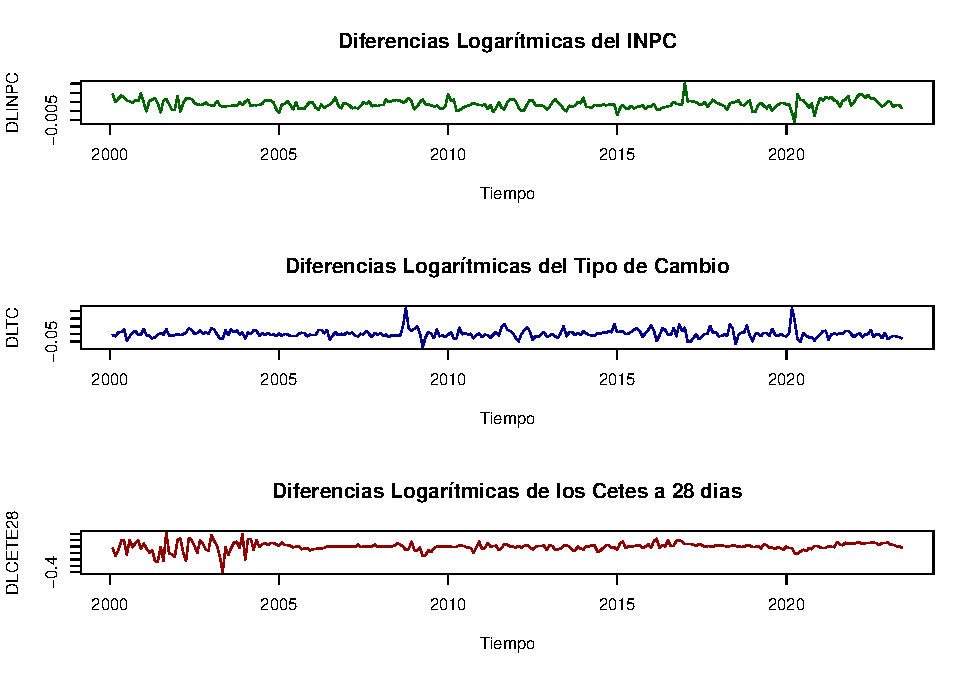
\includegraphics{Notas-Series-Tiempo_files/figure-latex/fig61-1} 

}

\caption{Series en diferencias logarítmicas dadas por las siguientes expresiones: $DLINPC_t = ln(DLINPC_t) - ln(DLINPC_{t-1})$, $DLTC_t = ln(TC_t) - ln(TC_{t-1})$ y $DLCETE28_t = ln(CETE28_t) - ln(CETE28_{t-1})$.}\label{fig:fig61}
\end{figure}

\begin{Shaded}
\begin{Highlighting}[]
\FunctionTok{par}\NormalTok{(}\AttributeTok{mfrow=}\FunctionTok{c}\NormalTok{(}\DecValTok{1}\NormalTok{, }\DecValTok{1}\NormalTok{))}

\CommentTok{\#dev.off()}
\end{Highlighting}
\end{Shaded}

Por simplicidad, en el Cuadro \ref{tab:Granger} se muestra el resultado
de aplicar el test de Granger a diferentes especificaciones, con rezagos
4, 8, 12 y 16, sólo para la serie de Tipo de Cambio en diferencias
logarítmicas. En cada una de las pruebas se compara el modelo
considerado como regresor a la variable que es candidata de causar,
respecto del modelo sin considerar a dicha variable.

\begin{longtable}[]{@{}cccc@{}}
\caption{\label{tab:Granger} Prueba de si \(DLINPC_t\) Granger causa a \(DLTC_t\).}\tabularnewline
\toprule\noalign{}
Rezagos & Estadiística F & Probabilidad (\(>\)F) & Significancia \\
\midrule\noalign{}
\endfirsthead
\toprule\noalign{}
Rezagos & Estadiística F & Probabilidad (\(>\)F) & Significancia \\
\midrule\noalign{}
\endhead
\bottomrule\noalign{}
\endlastfoot
4 & 3.2621 & 0.01265 & * \\
8 & 1.9079 & 0.06030 & \\
12 & 2.2577 & 0.01067 & * \\
16 & 1.6735 & 0.05495 & * \\
Notas: & *** & signif. & al 0.1\% \\
& ** & signif. & al 1\% \\
& * & signif. & al 5\% \\
\end{longtable}

De acuerdo con el Cuadro \ref{tab:Granger}, podemos concluir que existe
información estadísticamente significativa para concluir que la
inflación causa a la tasa de depreciación cambiaria, ambas medidas como
las diferencias logaritmicas. El resto de los resultados para las otras
combinaciones de causalidad se encuentran en el R Markdown llamado Clase
13 ubicado en el repositorio de GitHub.

\hypertarget{definiciuxf3n-y-representaciuxf3n-del-sistema-o-modelo-de-vectores-autorregresicos-varp}{%
\section{Definición y representación del Sistema o Modelo de Vectores Autorregresicos (VAR(p))}\label{definiciuxf3n-y-representaciuxf3n-del-sistema-o-modelo-de-vectores-autorregresicos-varp}}

En esta sección ampliaremos la discusión planteada en el apartado
anterior. En el sentido de que en la sección pasada nuestra discusión se
limitó al análisis de causalidad entre dos variables a la vez, que si
bien es posible extenderlo a más variables, es un procedimiento limitado
a casos particulares por las siguientes razones.

El procedimiento de causalidad de Granger supone que es posible
identificar un sistema de ecuaciones que debe conformarse una vez que se
ha identificado el sentido de la causalidad. Así, el proceso anterior
necesita del conocimiento previo de las relaciones que existen entre las
variables.

Adicionalmente, no resuelve el problema más general que está relacionado
con cómo identificar la causalidad cuando se tienen múltiples variables
con múltiples sentidos de causalidad. En esta sección analizaremos una
mejor aproximación al problema de cómo identificar la causalidad
múltiple. Por lo tanto, como mecanismo para solucionar el problema
planteado, analizaremos el caso de un Sistema o Modelo de Vectores
Autoregresivos conocido como VAR.

El primer supuesto del que partiremos es que existe algún grado de
endogeneidad entre las variables consideradas en el análisis.
Adicionalmente, el segundo supuesto que estableceremos es que requerimos
que las variables que tengamos consideradas sean estacionarias.

Por lo anterior, diremos que un modelo de Vectores Autoregresivos (VAR)
es un procedimiento que sigue fundado en el supuesto de que las
variables consideradas son estacionarias. Así, hasta este momento del
curso hemos pasado de modelos univariados a modelos multivariados, pero
no hemos podido dejar de asumir que las series son estacionarias.

En lo subsecuente asumiremos que las series empleadas son estacionarias
y sólo lo demostraremos cuando, en su caso, sea necesario. Esto no
significa que el lector deba asumir estacionariedad. Por el contrario,
siempre debe probar que las series son estacionarias antes de iniciar la
implementación de cualquier técnica de series de tiempo.

Ahora bien, iniciaremos con el establecimiento de la representación del
proceso. Digamos que tenemos un proceso estocástico \(\mathbf{X}_t\)
estacionario vectorial de dimensión \(k\): \begin{equation*}
    \mathbf{X}_t = 
    \begin{bmatrix}
    X_{1t} \\ X_{2t} \\ \vdots \\ X_{kt}
    \end{bmatrix}
\end{equation*}

Para cualquier \(i = 1, 2, \ldots, p\): \begin{equation*}
    \mathbf{X}_{t-i} = 
    \begin{bmatrix}
    X_{1t-i} \\ X_{2t-i} \\ \vdots \\ X_{kt-i}
    \end{bmatrix}
\end{equation*}

Donde cada \(X_{kt}\) en \(\mathbf{X}_t\) es una serie de tiempo por sí
misma. De esta forma, la expresión reducida del modelo o el proceso
\(VAR(p)\) estará dado por:
\begin{equation}
    \mathbf{X}_t = \boldsymbol{\delta} + A_1 \mathbf{X}_{t-1} + A_2 \mathbf{X}_{t-2} + \ldots + A_p \mathbf{X}_{t-p} + \mathbf{U}_{t}
    \label{eq:VARp}
\end{equation}

Donde cada uno de las \(A_i\), \(i = 1, 2, \ldots, p\), son matrices
cuadradas de dimensión \(k\) y \(\mathbf{U}_t\) representa un vector de
dimensión \(k \times 1\) con los residuales en el momento del tiempo \(t\)
que son, por individual, un proceso puramente aleatorio. También se
incorpora un vector de términos constantes denominado como
\(\mathbf{\delta}\), el cual es de dimensión \(k \times 1\).

Así, la ecuación \eqref{eq:VARp} supone la siguiente estructura del
vector \(\boldsymbol{\delta}\): \begin{equation*}
    \boldsymbol{\delta} = 
    \begin{bmatrix}
    \delta_{1} \\ \delta_{2} \\ \vdots \\ \delta_{k}
    \end{bmatrix}
\end{equation*}

También, la ecuación \eqref{eq:VARp} supone que cada matriz \(A_i\),
\(i = 1, 2, \ldots, p\) está definida de la siguiente forma:
\begin{equation*}
    \mathbf{A}_i = 
    \begin{bmatrix}
    a^{(i)}_{11} & a^{(i)}_{12} & \ldots & a^{(i)}_{1k} \\ a^{(i)}_{21} & a^{(i)}_{22} & \ldots & a^{(i)}_{2k} \\ \vdots & \vdots & \ddots & \vdots \\ a^{(i)}_{k1} & a^{(i)}_{k2} & \ldots & a^{(i)}_{kk}
    \end{bmatrix}
\end{equation*}

Donde \(i = 1, 2, \ldots, p\).

Retomando la ecuación \eqref{eq:VARp} y considerando que podemos ocupar
el operador rezago \(L^j\) de forma análoga al caso del modelo \(AR(p)\),
pero aplicado a un vector, tenemos las siguientes ecuaciones:
\begin{eqnarray}
    \mathbf{X}_t - A_1 \mathbf{X}_{t-1} - A_2 \mathbf{X}_{t-2} - \ldots - A_p \mathbf{X}_{t-p} & = & \boldsymbol{\delta} + \mathbf{U}_{t} \nonumber \\
    \mathbf{X}_t - A_1 L \mathbf{X}_{t} - A_2 L^2 \mathbf{X}_{t} - \ldots - A_p L^p \mathbf{X}_{t-p} & = & \boldsymbol{\delta} + \mathbf{U}_{t} \nonumber \\
    (I_k - \mathbf{A_1} L - \mathbf{A_2} L^2 - \ldots - \mathbf{A_p} L^p) \mathbf{X}_t & = & \boldsymbol{\delta} + \mathbf{U}_{t} \nonumber \\
    \mathbf{A}(L) \mathbf{X}_t & = & \boldsymbol{\delta} + \mathbf{U}_{t}
    \label{eq:VARCorto}
\end{eqnarray}

Adicionalmente, requeriremos que dado que \(\mathbf{U}_t\) es un proceso
puramente aleatorio, este debe cumplir con las siguientes condiciones:

\begin{enumerate}
\def\labelenumi{\arabic{enumi}.}
\item
  El valor esperado del término de error es cero: \begin{equation}
     \mathbb{E}[\mathbf{U}_t] = 0
    \end{equation}
\item
  Existe una matriz de varianzas y covarianzas entre los términos de
  error contemporáneos dada por:
  \begin{eqnarray}
     \mathbb{E}[\mathbf{U}_t \mathbf{U}_t'] 
     & = &
     \mathbb{E} \left[
     \begin{bmatrix}
     U^{(t)}_{1} \\ U^{(t)}_{2} \\ \vdots \\ U^{(t)}_{k}
     \end{bmatrix}
     \begin{bmatrix}
     U^{(t)}_{1} & U^{(t)}_{2} & \ldots & U^{(t)}_{k}
     \end{bmatrix}
     \right] \nonumber \\
     & = & \mathbb{E}
     \begin{bmatrix}
     U^{(t)}_{1} U^{(t)}_{1} & U^{(t)}_{1} U^{(t)}_{2} & \ldots & U^{(t)}_{1} U^{(t)}_{k} \\
     U^{(t)}_{2} U^{(t)}_{1} & U^{(t)}_{2} U^{(t)}_{2} & \ldots & U^{(t)}_{2} U^{(t)}_{k} \\
     \vdots & \vdots & \ldots & \vdots \\
     U^{(t)}_{k} U^{(t)}_{1} & U^{(t)}_{k} U^{(t)}_{2} & \ldots & U^{(t)}_{k} U^{(t)}_{k}
     \end{bmatrix} \nonumber \\
     & = & \begin{bmatrix}
     \sigma^2_1 & \rho_{12} & \ldots & \rho_{1k} \\
     \rho_{21} & \sigma^2_2 & \ldots & \rho_{2k} \\
     \vdots & \vdots & \ldots & \vdots \\
     \rho_{k1} & \rho_{k2} & \ldots & \sigma^2_k
     \end{bmatrix} \nonumber \\
     & = & \mathbf{\Sigma}_{UU}
     \label{eq:SigmaVAR}
    \end{eqnarray}
\item
  La matriz de varianzas y covarianzas no contemporáneas es nula. Es
  decir, que para todo \(t \neq s\):
  \begin{eqnarray}
      \mathbb{E} [\mathbf{U}_t \mathbf{U}_s'] 
      & = &
      \mathbb{E} \left[
      \begin{bmatrix}
      U^{(t)}_{1} \\ U^{(t)}_{2} \\ \vdots \\ U^{(t)}_{k}
      \end{bmatrix}
      \begin{bmatrix}
      U^{(s)}_{1} & U^{(s)}_{2} & \ldots & U^{(s)}_{k}
      \end{bmatrix}
      \right] \nonumber \\
      & =  & \mathbb{E}
      \begin{bmatrix}
      U^{(t)}_{1} U^{(s)}_{1} & U^{(t)}_{1} U^{(s)}_{2} & \ldots & U^{(t)}_{1} U^{(s)}_{k} \\
      U^{(t)}_{2} U^{(s)}_{1} & U^{(t)}_{2} U^{(s)}_{2} & \ldots & U^{(t)}_{2} U^{(s)}_{k} \\
      \vdots & \vdots & \ldots & \vdots \\
      U^{(t)}_{k} U^{(s)}_{1} & U^{(t)}_{k} U^{(s)}_{2} & \ldots & U^{(t)}_{k} U^{(s)}_{k}
      \end{bmatrix} \nonumber \\
      & = & \mathbf{0}
      \label{eq:RhoVAR}
  \end{eqnarray}
\end{enumerate}

Las ecuaciones \eqref{eq:SigmaVAR} y \eqref{eq:RhoVAR} significan que los
residuales \(\mathbf{U}_t\) pueden estar correlacionados entre ellos solo
en el caso de que la información sea contemporánea, pero no tienen
información en común entre residuales de otros periodos.

Al igual que en el caso del modelo o especificación \(AR(p)\) en la
especificación del modelo \(VAR(p)\) existen condiciones de estabilidad.
Dichas condiciones están dadas por lo siguiente, definamos el siguiente
polinomio que resulta de tomar la matriz \(\mathbf{A}(L)\) en la ecuación
\eqref{eq:VARCorto}: \begin{equation}
    Det[I_t - A_1 z - A_2 z^2 - \ldots - A_p z^p] \neq 0
\end{equation}

Donde las raíces del polinomio cumplen que \(|z| \leq 1\), es decir, se
ubican dentro del circulo unitario.

La ecuación \eqref{eq:VARCorto} puede ser rexpresada en una forma similar
al un proceso de MA. Al respecto, de forma similar a la siguiente
ecuación podemos construir un modelo \(VARMA(p,q)\), el cual no estudiamos
es este curso.

Reromando el primer planteamiento, podemos escribir:
\begin{eqnarray}
    \mathbf{X}_t & = & \mathbf{A}^{-1}(L) \boldsymbol{\delta} + \mathbf{A}^{-1}(L) \mathbf{U}_t \nonumber \\
    & = & \boldsymbol{\mu} + \boldsymbol{\beta}(L) \mathbf{U}_t
    \label{eq:VARMAq}
\end{eqnarray}

Donde \(\boldsymbol{\mu}\) es un vector de \(k \times 1\) constantes y
\(\boldsymbol{\beta}(L)\) es una matriz que depende de \(L\).

Por el lado de las matrices que representan la autocovarianza, estás
resultan de resolver lo siguiente: \begin{equation}
    \Gamma_X(\tau) = E[(\mathbf{X}_t - \mu)(\mathbf{X}_{t-\tau} - \mu)'] 
\end{equation}

Ahora, sin pérdida de generalidad digamos que la especificación VAR(p)
en la ecuación \eqref{eq:VARp} no tiene constante, por lo que
\(\boldsymbol{\delta} = \mathbf{0}\), lo que implica que
\(\boldsymbol{\mu} = \mathbf{0}\). De esta forma las matrices de
autocovarianza resultan de: \begin{eqnarray*}
    \Gamma_{\mathbf{X}}(\tau) & = & E[(\mathbf{X}_t)(\mathbf{X}_{t-\tau})'] \\
    & = & \mathbf{A_1} E[(\mathbf{X}_{t-1})(\mathbf{X}_{t-\tau})'] + \mathbf{A_2} E[(\mathbf{X}_{t-2})(\mathbf{X}_{t-\tau})'] \\
    &   & + \ldots + \mathbf{A_p} E[(\mathbf{X}_{t-p})(\mathbf{X}_{t-\tau})'] + E[(\mathbf{U}_t(\mathbf{X}_{t-\tau})']
\end{eqnarray*}

Finalmente, al igual que en el caso \(AR(p)\), requerimos de una métrica
que nos permita determinar el número de rezagos óptimo \(p\) en el
\(VAR(p)\). Así, establecemos criterios de información similares a los del
\(AR(p)\) dados por:

1.Final Prediction Error (FPE): \begin{equation}
        FPE(p) = \left[ \frac{T + kp + 1}{T - kp - 1} \right]^k |\mathbf{\Sigma}_{\hat{U}\hat{U}}(p)|
        \end{equation}

\begin{enumerate}
\def\labelenumi{\arabic{enumi}.}
\setcounter{enumi}{1}
\item
  Akaike Criterion (AIC): \begin{equation}
       AIC(p) = ln|\mathbf{\Sigma}_{\hat{U}\hat{U}}(p)| + (k + p k^2) \frac{2}{T}
       \end{equation}
\item
  Hannan - Quinn Criterion (HQ): \begin{equation}
       HQ(p) = ln|\mathbf{\Sigma}_{\hat{U}\hat{U}}(p)| + (k + p k^2) \frac{2ln(ln(2))}{T}
       \end{equation}
\item
  Schwartz Criterion (SC): \begin{equation}
       SC(p) = ln|\mathbf{\Sigma}_{\hat{U}\hat{U}}(p)| + (k + p k^2) \frac{ln(T)}{T}
       \end{equation}
\end{enumerate}

Donde la matriz de varianzas y covarianzas contemporáneas estará dada
por: \begin{equation*}
            \mathbf{\Sigma}_{\hat{U}\hat{U}}(p) = \mathbb{E} \left[
            \begin{bmatrix}
            U^{(t)}_{1} \\ U^{(t)}_{2} \\ \vdots \\ U^{(t)}_{k}
            \end{bmatrix}
            \begin{bmatrix}
            U^{(t)}_{1} & U^{(t)}_{2} & \ldots & U^{(t)}_{k}
            \end{bmatrix}
            \right]
    \end{equation*}

\textbf{Ejemplo}. Ahora veámos un ejemplo de estimación de \(VAR(p)\).
Para el ejemplo utilizaremos las series de INPC, Tipo de Cambio,
rendimiento de los Cetes a 28 días, el IGAE y el Índice de Producción
Industrial de los Estados Unidos, todas desestacionalizadas y para el
período de enero de 2000 a julio de 2019. Dado que el supuesto
estacionariedad sigue presente en nuestro análisis, emplearemos cada una
de las series en su versión de diferencias logaritmicas. Las Figuras
\ref{fig:fig62} y \ref{fig:fig63} muestra las series referidas.

\begin{Shaded}
\begin{Highlighting}[]
\FunctionTok{library}\NormalTok{(ggplot2)}
\FunctionTok{library}\NormalTok{(dplyr)}
\FunctionTok{library}\NormalTok{(stats)}
\FunctionTok{library}\NormalTok{(MASS)}
\FunctionTok{library}\NormalTok{(strucchange)}
\FunctionTok{library}\NormalTok{(zoo)}
\FunctionTok{library}\NormalTok{(sandwich)}
\FunctionTok{library}\NormalTok{(urca)}
\FunctionTok{library}\NormalTok{(lmtest)}
\FunctionTok{library}\NormalTok{(vars)}

\CommentTok{\#}
\FunctionTok{load}\NormalTok{(}\StringTok{"BD/Datos\_Ad.RData"}\NormalTok{)}

\CommentTok{\#}
\NormalTok{DLINPC }\OtherTok{\textless{}{-}} \FunctionTok{diff}\NormalTok{(}\FunctionTok{log}\NormalTok{( }\FunctionTok{ts}\NormalTok{(Datos\_Ad}\SpecialCharTok{$}\NormalTok{INPC\_Ad, }\AttributeTok{start =} \FunctionTok{c}\NormalTok{(}\DecValTok{2000}\NormalTok{, }\DecValTok{1}\NormalTok{), }\AttributeTok{freq =} \DecValTok{12}\NormalTok{) ))}

\NormalTok{DLTC }\OtherTok{\textless{}{-}} \FunctionTok{diff}\NormalTok{(}\FunctionTok{log}\NormalTok{( }\FunctionTok{ts}\NormalTok{(Datos\_Ad}\SpecialCharTok{$}\NormalTok{TC\_Ad, }\AttributeTok{start =} \FunctionTok{c}\NormalTok{(}\DecValTok{2000}\NormalTok{, }\DecValTok{1}\NormalTok{), }\AttributeTok{freq =} \DecValTok{12}\NormalTok{) ))}

\NormalTok{DLCETE28 }\OtherTok{\textless{}{-}} \FunctionTok{diff}\NormalTok{(}\FunctionTok{log}\NormalTok{( }\FunctionTok{ts}\NormalTok{(Datos\_Ad}\SpecialCharTok{$}\NormalTok{CETE28\_Ad, }\AttributeTok{start =} \FunctionTok{c}\NormalTok{(}\DecValTok{2000}\NormalTok{, }\DecValTok{1}\NormalTok{), }\AttributeTok{freq =} \DecValTok{12}\NormalTok{) ))}

\NormalTok{DLIGAE }\OtherTok{\textless{}{-}} \FunctionTok{diff}\NormalTok{(}\FunctionTok{log}\NormalTok{( }\FunctionTok{ts}\NormalTok{(Datos\_Ad}\SpecialCharTok{$}\NormalTok{IGAE\_Ad, }\AttributeTok{start =} \FunctionTok{c}\NormalTok{(}\DecValTok{2000}\NormalTok{, }\DecValTok{1}\NormalTok{), }\AttributeTok{freq =} \DecValTok{12}\NormalTok{) ))}

\NormalTok{DLIPI }\OtherTok{\textless{}{-}} \FunctionTok{diff}\NormalTok{(}\FunctionTok{log}\NormalTok{( }\FunctionTok{ts}\NormalTok{(Datos\_Ad}\SpecialCharTok{$}\NormalTok{IPI\_Ad, }\AttributeTok{start =} \FunctionTok{c}\NormalTok{(}\DecValTok{2000}\NormalTok{, }\DecValTok{1}\NormalTok{), }\AttributeTok{freq =} \DecValTok{12}\NormalTok{) ))}

\NormalTok{Datos }\OtherTok{\textless{}{-}} \FunctionTok{data.frame}\NormalTok{(}\FunctionTok{cbind}\NormalTok{(DLINPC, DLTC, DLCETE28, DLIGAE, DLIPI))}

\NormalTok{Datos }\OtherTok{\textless{}{-}} \FunctionTok{ts}\NormalTok{(Datos, }
            \AttributeTok{start =} \FunctionTok{c}\NormalTok{(}\DecValTok{2000}\NormalTok{, }\DecValTok{2}\NormalTok{), }\AttributeTok{freq =} \DecValTok{12}\NormalTok{)}
\end{Highlighting}
\end{Shaded}

\begin{Shaded}
\begin{Highlighting}[]
\FunctionTok{plot}\NormalTok{(Datos, }\AttributeTok{plot.type =} \StringTok{"s"}\NormalTok{, }
     \AttributeTok{col =} \FunctionTok{c}\NormalTok{(}\StringTok{"darkgreen"}\NormalTok{, }\StringTok{"darkblue"}\NormalTok{, }\StringTok{"darkred"}\NormalTok{, }\StringTok{"black"}\NormalTok{, }\StringTok{"purple"}\NormalTok{), }
     \AttributeTok{main =} \StringTok{"Series en Diferencias logaritmicas"}\NormalTok{, }
     \AttributeTok{xlab =} \StringTok{"Tiempo"}\NormalTok{, }\AttributeTok{ylab =} \StringTok{"Variacion"}\NormalTok{)}

\FunctionTok{legend}\NormalTok{(}\StringTok{"bottomright"}\NormalTok{, }\FunctionTok{c}\NormalTok{(}\StringTok{"INPC"}\NormalTok{, }\StringTok{"TC"}\NormalTok{, }\StringTok{"CETES28"}\NormalTok{, }\StringTok{"IGAE"}\NormalTok{, }\StringTok{"IPI"}\NormalTok{),}
       \AttributeTok{cex =} \FloatTok{0.6}\NormalTok{, }\AttributeTok{lty =} \DecValTok{1}\SpecialCharTok{:}\DecValTok{1}\NormalTok{, }
       \AttributeTok{col =} \FunctionTok{c}\NormalTok{(}\StringTok{"darkgreen"}\NormalTok{, }\StringTok{"darkblue"}\NormalTok{, }\StringTok{"darkred"}\NormalTok{, }\StringTok{"black"}\NormalTok{, }\StringTok{"purple"}\NormalTok{))}
\end{Highlighting}
\end{Shaded}

\begin{figure}

{\centering 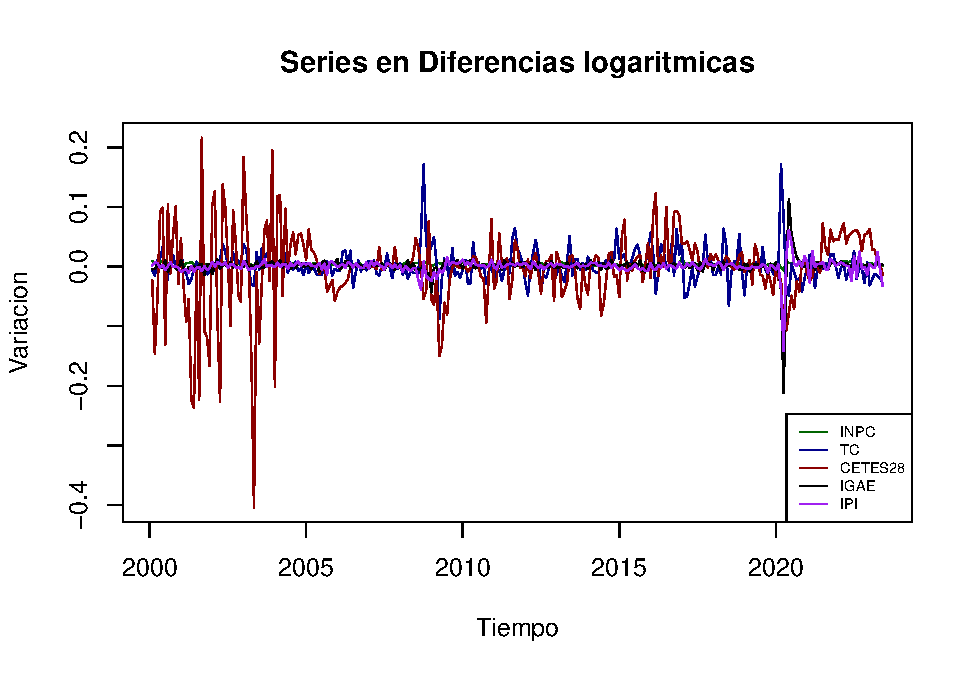
\includegraphics{Notas-Series-Tiempo_files/figure-latex/fig62-1} 

}

\caption{Series en diferencias logarítmicas (Forma 1)}\label{fig:fig62}
\end{figure}

\begin{Shaded}
\begin{Highlighting}[]
\FunctionTok{plot}\NormalTok{(Datos, }\AttributeTok{plot.type =} \StringTok{"m"}\NormalTok{, }
     \AttributeTok{col =} \StringTok{"darkgreen"}\NormalTok{, }
     \AttributeTok{main =} \StringTok{"Series en Diferencias logaritmicas"}\NormalTok{, }\AttributeTok{xlab =} \StringTok{"Tiempo"}\NormalTok{)}
\end{Highlighting}
\end{Shaded}

\begin{figure}

{\centering 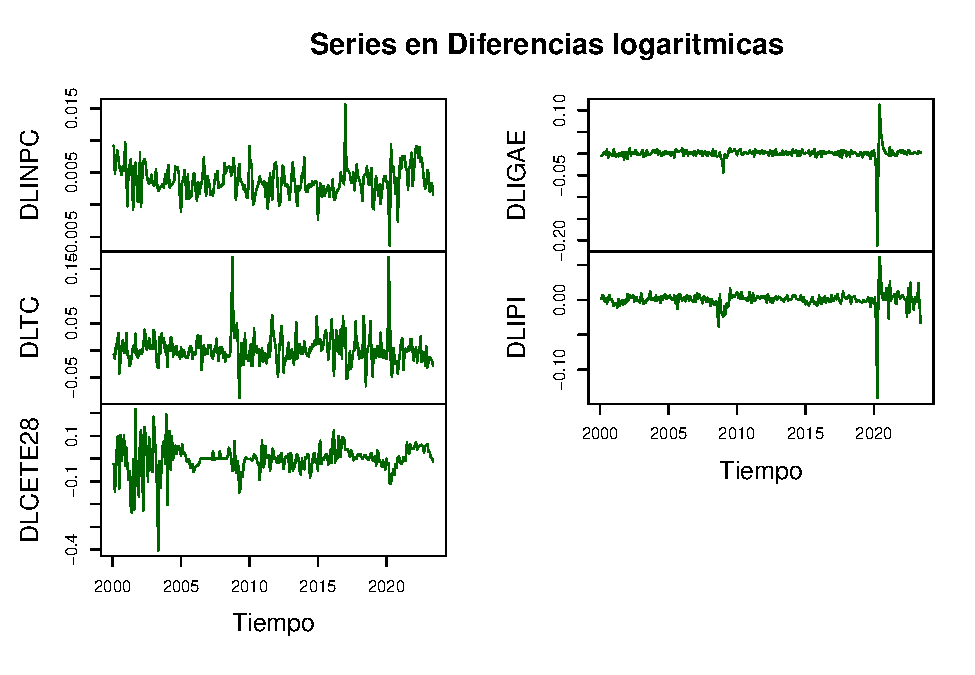
\includegraphics{Notas-Series-Tiempo_files/figure-latex/fig63-1} 

}

\caption{Series en diferencias logarítmicas (Forma 2)}\label{fig:fig63}
\end{figure}

Dicho lo anterior, a continuación mostraremos la tabla que resume el
valor de los distintos criterios de información para una especificación
de un \(VAR(p)\) con constante. Notése que es posible especificar un
\(VAR(p)\) con tendencia, siempre que exista evidencia de que algunas de
las series sean estacionarias alrededor de una tendencia. Caso que no
aplica hasta este momento, ya que nuestro análisis de estacionariedad es
claro respecto a la media constante (más adelante aportaremos la
evidencia de esto), lo cual elimina la posibilidad de incluir una
tendencia.

En el Cuadro \ref{tab:NumSelectVAR} reportamos el número de rezagos
propuesto a partir de cada criterio de información y en el Cuadro
\ref{tab:SelectVAR} reportamos los resultados de aplicar una prueba de
criterios de información para diferentes valores de rezagos. Del cual se
concluye que el número óptimo de rezagos es 2 (según el criterio AIC y
el FPE) y 1 (según el criterio HQ y el SC). Recordemos que es común que
el criterio AIC siempre reporte el mayor valor de rezagos, por lo que es
una buena práctica utilizarlo como referente principal.

\begin{longtable}[]{@{}cccc@{}}
\caption{\label{tab:NumSelectVAR} Número de rezagos determinados por cada uno de los
criterios de información para diferentes especificaciones de modelos
VAR(p) con término constante de la series \(DLINPC_t\), \(DLTC_t\),
\(DLCETE28_t\), \(DLIGAE_t\) y \(DLIPI_t\).}\tabularnewline
\toprule\noalign{}
\textbf{AIC} & \textbf{HQ} & \textbf{SC} & \textbf{FPE} \\
\midrule\noalign{}
\endfirsthead
\toprule\noalign{}
\textbf{AIC} & \textbf{HQ} & \textbf{SC} & \textbf{FPE} \\
\midrule\noalign{}
\endhead
\bottomrule\noalign{}
\endlastfoot
2 & 1 & 1 & 2 \\
\end{longtable}

\begin{longtable}[]{@{}
  >{\centering\arraybackslash}p{(\columnwidth - 8\tabcolsep) * \real{0.1449}}
  >{\centering\arraybackslash}p{(\columnwidth - 8\tabcolsep) * \real{0.2174}}
  >{\centering\arraybackslash}p{(\columnwidth - 8\tabcolsep) * \real{0.2174}}
  >{\centering\arraybackslash}p{(\columnwidth - 8\tabcolsep) * \real{0.2174}}
  >{\centering\arraybackslash}p{(\columnwidth - 8\tabcolsep) * \real{0.2029}}@{}}
\caption{\label{tab:SelectVAR} Criterios de información para diferentes
especificaciones de modelos VAR(p) con término constante de la series
\(DLINPC_t\), \(DLTC_t\), \(DLCETE28_t\), \(DLIGAE_t\) y \(DLIPI_t\).}\tabularnewline
\toprule\noalign{}
\begin{minipage}[b]{\linewidth}\centering
Rezagos
\end{minipage} & \begin{minipage}[b]{\linewidth}\centering
AIC
\end{minipage} & \begin{minipage}[b]{\linewidth}\centering
HQ
\end{minipage} & \begin{minipage}[b]{\linewidth}\centering
SC
\end{minipage} & \begin{minipage}[b]{\linewidth}\centering
FPE
\end{minipage} \\
\midrule\noalign{}
\endfirsthead
\toprule\noalign{}
\begin{minipage}[b]{\linewidth}\centering
Rezagos
\end{minipage} & \begin{minipage}[b]{\linewidth}\centering
AIC
\end{minipage} & \begin{minipage}[b]{\linewidth}\centering
HQ
\end{minipage} & \begin{minipage}[b]{\linewidth}\centering
SC
\end{minipage} & \begin{minipage}[b]{\linewidth}\centering
FPE
\end{minipage} \\
\midrule\noalign{}
\endhead
\bottomrule\noalign{}
\endlastfoot
1 & -4.636412e+01 & -4.617847e+01 & -4.590430e+01 & 7.317262e-21 \\
2 & -4.639541e+01 & -4.605506e+01 & -4.555241e+01 & 7.094216e-21 \\
3 & -4.635305e+01 & -4.585799e+01 & -4.512686e+01 & 7.407479e-21 \\
\(\vdots\) & \(\vdots\) & \(\vdots\) & \(\vdots\) & \(\vdots\) \\
\end{longtable}

\begin{Shaded}
\begin{Highlighting}[]
\FunctionTok{VARselect}\NormalTok{(Datos, }\AttributeTok{lag.max =} \DecValTok{12}\NormalTok{, }\AttributeTok{type =} \StringTok{"const"}\NormalTok{)}
\end{Highlighting}
\end{Shaded}

\begin{verbatim}
## $selection
## AIC(n)  HQ(n)  SC(n) FPE(n) 
##      2      1      1      2 
## 
## $criteria
##                                    1                             2
## AIC(n) -43.4369385930444451560106245 -43.4878280980991220872056147
## HQ(n)  -43.2759374580961733158801508 -43.1926593506939511257769482
## SC(n)  -43.0360414131631969780755753 -42.7528499349835016118959174
## FPE(n)   0.0000000000000000001366449   0.0000000000000000001298899
##                                    3                             4
## AIC(n) -43.4268489491758202802884625 -43.3868843889051234441467386
## HQ(n)  -42.9975125893137573029889609 -42.8233804165861613455490442
## SC(n)  -42.3577898028258275076041173 -41.9837442593207583740877453
## FPE(n)   0.0000000000000000001381225   0.0000000000000000001438821
##                                   5                             6
## AIC(n) -43.293163285544032703455741 -43.2431704133633161291072611
## HQ(n)  -42.595491700768178588987212 -42.4113312161305699987678963
## SC(n)  -41.555942172725302441449458 -41.1718683173102135697263293
## FPE(n)   0.000000000000000000158246   0.0000000000000000001667106
##                                    7                             8
## AIC(n) -43.2902076769675190348607430 -43.2419352439015938216471113
## HQ(n)  -42.3242008672778737832231855 -42.1417608217550565541387186
## SC(n)  -40.8848245976800441781051632 -40.5024711813797466675168835
## FPE(n)   0.0000000000000000001595179   0.0000000000000000001680601
##                                    9                            10
## AIC(n) -43.2201406224138153788771888 -43.1788072276712782127106038
## HQ(n)  -41.9857985878103789900706033 -41.8102975806109569134605408
## SC(n)  -40.1465955766575959273723129 -39.7711811986806935692584375
## FPE(n)   0.0000000000000000001726236   0.0000000000000000001810365
##                                   11                            12
## AIC(n) -43.1191364389135785017970193 -43.0502244962885995960277796
## HQ(n)  -41.6164591793963580812487635 -41.4133796243144800541813311
## SC(n)  -39.3774294266886144555428473 -38.9744365008292632523989596
## FPE(n)   0.0000000000000000001936459   0.0000000000000000002093856
\end{verbatim}

De esta forma, justificamos la estimación de un \(VAR(2)\). Los resultados
del mismo se reportan en los siguientes cuadros, en los que se muestra
el resultado de una de las ecuaciones. Los resultados restantes se
encuentran en el código de R mostrado más abajo. Primero mostraremos los
resultados de las raíces del polinomio característico en el Cuadro
\ref{tab:RootsVAR}, seguido de un cuadro para la ecuación del IGAE en
el Cuadro \ref{tab:IGAEVAR} (por simplicidad se omiten las otras cuatro
ecuaciones del VAR(2)), y del Cuadro \ref{tab:SigmaVARp} con la matriz
\(\mathbf{\Sigma}_{\hat{U}\hat{U}}\) estimada del VAR.

\begin{longtable}[]{@{}ccccc@{}}
\caption{\label{tab:RootsVAR} Raíces del polinomio característico de un VAR(2).}\tabularnewline
\toprule\noalign{}
\endfirsthead
\endhead
\bottomrule\noalign{}
\endlastfoot
0.7452 & 0.4403 & 0.4403 & 0.3503 & 0.3503 \\
0.3342 & 0.3342 & 0.3339 & 0.3339 & 0.06951 \\
\end{longtable}

\begin{longtable}[]{@{}
  >{\centering\arraybackslash}p{(\columnwidth - 8\tabcolsep) * \real{0.2571}}
  >{\centering\arraybackslash}p{(\columnwidth - 8\tabcolsep) * \real{0.1857}}
  >{\centering\arraybackslash}p{(\columnwidth - 8\tabcolsep) * \real{0.1714}}
  >{\centering\arraybackslash}p{(\columnwidth - 8\tabcolsep) * \real{0.1429}}
  >{\centering\arraybackslash}p{(\columnwidth - 8\tabcolsep) * \real{0.2429}}@{}}
\caption{\label{tab:IGAEVAR} Criterios de información para diferentes
especificaciones de modelos VAR(p) con término constante de la series
\(DLINPC_t\), \(DLTC_t\), \(DLCETE28_t\), \(DLIGAE_t\) y \(DLIPI_t\).}\tabularnewline
\toprule\noalign{}
\begin{minipage}[b]{\linewidth}\centering
Variable
\end{minipage} & \begin{minipage}[b]{\linewidth}\centering
Coeficiente
\end{minipage} & \begin{minipage}[b]{\linewidth}\centering
Error Est.
\end{minipage} & \begin{minipage}[b]{\linewidth}\centering
Estad. t
\end{minipage} & \begin{minipage}[b]{\linewidth}\centering
Prob.(\(>\) t)
\end{minipage} \\
\midrule\noalign{}
\endfirsthead
\toprule\noalign{}
\begin{minipage}[b]{\linewidth}\centering
Variable
\end{minipage} & \begin{minipage}[b]{\linewidth}\centering
Coeficiente
\end{minipage} & \begin{minipage}[b]{\linewidth}\centering
Error Est.
\end{minipage} & \begin{minipage}[b]{\linewidth}\centering
Estad. t
\end{minipage} & \begin{minipage}[b]{\linewidth}\centering
Prob.(\(>\) t)
\end{minipage} \\
\midrule\noalign{}
\endhead
\bottomrule\noalign{}
\endlastfoot
\(DLINPC_{t-1}\) & -0.2584978 & 0.1658396 & -1.559 & 0.120493 \\
\(DLTC_{t-1}\) & 0.0022016 & 0.0152876 & 0.144 & 0.885620 \\
\(DLCETE28_{t-1}\) & 0.0009547 & 0.0049115 & 0.194 & 0.846054 \\
\(DLIGAE_{t-1}\) & -0.2351453 & 0.0699797 & -3.360 & 0.000917 *** \\
\(DLIPI_{t-1}\) & 0.2442406 & 0.0600502 & 4.067 & 6.62e-05 *** \\
\(DLINPC_{t-2}\) & -0.0775039 & 0.1694809 & -0.457 & 0.647904 \\
\(DLTC_{t-2}\) & -0.0413316 & 0.0144650 & -2.857 & 0.004680 ** \\
\(DLCETE28_{t-2}\) & 0.0005341 & 0.0048058 & 0.111 & 0.911612 \\
\(DLIGAE_{t-2}\) & -0.0646890 & 0.0693711 & -0.933 & 0.352092 \\
\(DLIPI_{t-2}\) & 0.1796286 & 0.0620861 & 2.893 & 0.004195 ** \\
\(\delta_4\) & 0.0030377 & 0.0008077 & 3.761 & 0.000217 *** \\
& Notas: & *** & signif. & al 0.1\% \\
& & ** & signif. & al 1\% \\
& & * & signif. & al 5\% \\
\end{longtable}

\begin{longtable}[]{@{}
  >{\centering\arraybackslash}p{(\columnwidth - 10\tabcolsep) * \real{0.1714}}
  >{\centering\arraybackslash}p{(\columnwidth - 10\tabcolsep) * \real{0.1714}}
  >{\centering\arraybackslash}p{(\columnwidth - 10\tabcolsep) * \real{0.1429}}
  >{\centering\arraybackslash}p{(\columnwidth - 10\tabcolsep) * \real{0.1714}}
  >{\centering\arraybackslash}p{(\columnwidth - 10\tabcolsep) * \real{0.1714}}
  >{\centering\arraybackslash}p{(\columnwidth - 10\tabcolsep) * \real{0.1714}}@{}}
\caption{\label{tab:SigmaVARp} Matriz \(\mathbf{\Sigma}_{\hat{U}\hat{U}}\) estimada
del VAR(2).}\tabularnewline
\toprule\noalign{}
\endfirsthead
\endhead
\bottomrule\noalign{}
\endlastfoot
& \(DLINPC_t\) & \(DLTC_t\) & \(DLCE28_t\) & \(DLIGAE_t\) & \(DLIGAE_t\) \\
\(DLINPC_t\) & 3.95e-06 & 3.19e-06 & -1.83e-06 & -5.29-07 & 1.34e-06 \\
\(DLTC_t\) & 3.19e-06 & 5.04e-04 & 4.27e-04 & 9.81e-06 & 1.61e-05 \\
\(DLCE28_t\) & -1.83e-06 & 4.27e-04 & 4.63e-03 & 1.26e-05 & 2.76e-05 \\
\(DLIGAE_t\) & -5.29e-07 & 9.81e-06 & 1.26e-05 & 2.43e-05 & 8.75e-06 \\
\(DLIGAE_t\) & 1.34e-06 & 1.61e-05 & 2.76e-05 & 8.75e-06 & 3.13e-05 \\
\end{longtable}

\begin{Shaded}
\begin{Highlighting}[]
\NormalTok{VAR\_p }\OtherTok{\textless{}{-}} \FunctionTok{VAR}\NormalTok{(Datos, }\AttributeTok{p =} \DecValTok{2}\NormalTok{, }\AttributeTok{type =} \StringTok{"const"}\NormalTok{)}

\FunctionTok{summary}\NormalTok{(VAR\_p)}
\end{Highlighting}
\end{Shaded}

\begin{verbatim}
## 
## VAR Estimation Results:
## ========================= 
## Endogenous variables: DLINPC, DLTC, DLCETE28, DLIGAE, DLIPI 
## Deterministic variables: const 
## Sample size: 279 
## Log Likelihood: 4142.895 
## Roots of the characteristic polynomial:
##  0.53  0.53 0.4501 0.4501 0.4425 0.4425 0.3251 0.3251 0.1677 0.1677
## Call:
## VAR(y = Datos, p = 2, type = "const")
## 
## 
## Estimation results for equation DLINPC: 
## ======================================= 
## DLINPC = DLINPC.l1 + DLTC.l1 + DLCETE28.l1 + DLIGAE.l1 + DLIPI.l1 + DLINPC.l2 + DLTC.l2 + DLCETE28.l2 + DLIGAE.l2 + DLIPI.l2 + const 
## 
##              Estimate Std. Error t value           Pr(>|t|)    
## DLINPC.l1    0.387061   0.063100   6.134 0.0000000030610259 ***
## DLTC.l1     -0.004611   0.005286  -0.872             0.3839    
## DLCETE28.l1  0.001229   0.002078   0.592             0.5546    
## DLIGAE.l1   -0.022088   0.015077  -1.465             0.1441    
## DLIPI.l1     0.009878   0.019363   0.510             0.6104    
## DLINPC.l2   -0.006707   0.063621  -0.105             0.9161    
## DLTC.l2      0.009608   0.005496   1.748             0.0816 .  
## DLCETE28.l2  0.001827   0.002051   0.891             0.3737    
## DLIGAE.l2    0.006544   0.014289   0.458             0.6473    
## DLIPI.l2    -0.015245   0.019632  -0.777             0.4381    
## const        0.002325   0.000294   7.908 0.0000000000000688 ***
## ---
## Signif. codes:  0 '***' 0.001 '**' 0.01 '*' 0.05 '.' 0.1 ' ' 1
## 
## 
## Residual standard error: 0.002176 on 268 degrees of freedom
## Multiple R-Squared: 0.1783,  Adjusted R-squared: 0.1476 
## F-statistic: 5.815 on 10 and 268 DF,  p-value: 0.00000006289 
## 
## 
## Estimation results for equation DLTC: 
## ===================================== 
## DLTC = DLINPC.l1 + DLTC.l1 + DLCETE28.l1 + DLIGAE.l1 + DLIPI.l1 + DLINPC.l2 + DLTC.l2 + DLCETE28.l2 + DLIGAE.l2 + DLIPI.l2 + const 
## 
##              Estimate Std. Error t value   Pr(>|t|)    
## DLINPC.l1   -1.344803   0.745382  -1.804    0.07233 .  
## DLTC.l1      0.315786   0.062442   5.057 0.00000079 ***
## DLCETE28.l1 -0.039912   0.024542  -1.626    0.10506    
## DLIGAE.l1    0.379306   0.178102   2.130    0.03411 *  
## DLIPI.l1    -0.514827   0.228727  -2.251    0.02521 *  
## DLINPC.l2    0.071779   0.751538   0.096    0.92398    
## DLTC.l2     -0.183813   0.064926  -2.831    0.00499 ** 
## DLCETE28.l2  0.030125   0.024228   1.243    0.21481    
## DLIGAE.l2    0.070713   0.168797   0.419    0.67561    
## DLIPI.l2    -0.166610   0.231909  -0.718    0.47312    
## const        0.006463   0.003473   1.861    0.06388 .  
## ---
## Signif. codes:  0 '***' 0.001 '**' 0.01 '*' 0.05 '.' 0.1 ' ' 1
## 
## 
## Residual standard error: 0.0257 on 268 degrees of freedom
## Multiple R-Squared: 0.1425,  Adjusted R-squared: 0.1105 
## F-statistic: 4.454 on 10 and 268 DF,  p-value: 0.000008102 
## 
## 
## Estimation results for equation DLCETE28: 
## ========================================= 
## DLCETE28 = DLINPC.l1 + DLTC.l1 + DLCETE28.l1 + DLIGAE.l1 + DLIPI.l1 + DLINPC.l2 + DLTC.l2 + DLCETE28.l2 + DLIGAE.l2 + DLIPI.l2 + const 
## 
##              Estimate Std. Error t value Pr(>|t|)  
## DLINPC.l1    3.933798   1.861561   2.113   0.0355 *
## DLTC.l1      0.112997   0.155945   0.725   0.4693  
## DLCETE28.l1  0.113300   0.061292   1.849   0.0656 .
## DLIGAE.l1   -0.588758   0.444803  -1.324   0.1868  
## DLIPI.l1     1.174496   0.571237   2.056   0.0407 *
## DLINPC.l2   -2.213087   1.876936  -1.179   0.2394  
## DLTC.l2      0.117661   0.162151   0.726   0.4687  
## DLCETE28.l2  0.063398   0.060509   1.048   0.2957  
## DLIGAE.l2   -0.237974   0.421565  -0.565   0.5729  
## DLIPI.l2     1.110203   0.579183   1.917   0.0563 .
## const       -0.007514   0.008674  -0.866   0.3872  
## ---
## Signif. codes:  0 '***' 0.001 '**' 0.01 '*' 0.05 '.' 0.1 ' ' 1
## 
## 
## Residual standard error: 0.06419 on 268 degrees of freedom
## Multiple R-Squared: 0.08823, Adjusted R-squared: 0.05421 
## F-statistic: 2.593 on 10 and 268 DF,  p-value: 0.005122 
## 
## 
## Estimation results for equation DLIGAE: 
## ======================================= 
## DLIGAE = DLINPC.l1 + DLTC.l1 + DLCETE28.l1 + DLIGAE.l1 + DLIPI.l1 + DLINPC.l2 + DLTC.l2 + DLCETE28.l2 + DLIGAE.l2 + DLIPI.l2 + const 
## 
##              Estimate Std. Error t value       Pr(>|t|)    
## DLINPC.l1    0.719855   0.393617   1.829         0.0685 .  
## DLTC.l1     -0.218508   0.032974  -6.627 0.000000000188 ***
## DLCETE28.l1  0.007718   0.012960   0.596         0.5520    
## DLIGAE.l1    0.037559   0.094051   0.399         0.6900    
## DLIPI.l1     0.389894   0.120785   3.228         0.0014 ** 
## DLINPC.l2   -0.737653   0.396868  -1.859         0.0642 .  
## DLTC.l2      0.073830   0.034286   2.153         0.0322 *  
## DLCETE28.l2 -0.013542   0.012794  -1.058         0.2908    
## DLIGAE.l2   -0.142845   0.089138  -1.603         0.1102    
## DLIPI.l2    -0.154835   0.122465  -1.264         0.2072    
## const        0.001637   0.001834   0.893         0.3729    
## ---
## Signif. codes:  0 '***' 0.001 '**' 0.01 '*' 0.05 '.' 0.1 ' ' 1
## 
## 
## Residual standard error: 0.01357 on 268 degrees of freedom
## Multiple R-Squared: 0.3272,  Adjusted R-squared: 0.3021 
## F-statistic: 13.03 on 10 and 268 DF,  p-value: < 0.00000000000000022 
## 
## 
## Estimation results for equation DLIPI: 
## ====================================== 
## DLIPI = DLINPC.l1 + DLTC.l1 + DLCETE28.l1 + DLIGAE.l1 + DLIPI.l1 + DLINPC.l2 + DLTC.l2 + DLCETE28.l2 + DLIGAE.l2 + DLIPI.l2 + const 
## 
##              Estimate Std. Error t value      Pr(>|t|)    
## DLINPC.l1    0.042383   0.326611   0.130        0.8968    
## DLTC.l1     -0.163742   0.027361  -5.985 0.00000000693 ***
## DLCETE28.l1  0.012143   0.010754   1.129        0.2598    
## DLIGAE.l1    0.098821   0.078041   1.266        0.2065    
## DLIPI.l1     0.067742   0.100224   0.676        0.4997    
## DLINPC.l2   -0.524835   0.329309  -1.594        0.1122    
## DLTC.l2      0.053353   0.028449   1.875        0.0618 .  
## DLCETE28.l2 -0.016237   0.010616  -1.529        0.1273    
## DLIGAE.l2   -0.088483   0.073964  -1.196        0.2326    
## DLIPI.l2    -0.082982   0.101618  -0.817        0.4149    
## const        0.002361   0.001522   1.551        0.1220    
## ---
## Signif. codes:  0 '***' 0.001 '**' 0.01 '*' 0.05 '.' 0.1 ' ' 1
## 
## 
## Residual standard error: 0.01126 on 268 degrees of freedom
## Multiple R-Squared: 0.1978,  Adjusted R-squared: 0.1679 
## F-statistic:  6.61 on 10 and 268 DF,  p-value: 0.000000003715 
## 
## 
## 
## Covariance matrix of residuals:
##                 DLINPC          DLTC    DLCETE28       DLIGAE       DLIPI
## DLINPC    0.0000047345 -0.0000001939 0.000004559  0.000006652  0.00000700
## DLTC     -0.0000001939  0.0006606619 0.000369751 -0.000035441 -0.00003174
## DLCETE28  0.0000045591  0.0003697510 0.004120747  0.000063618  0.00008525
## DLIGAE    0.0000066522 -0.0000354410 0.000063618  0.000184234  0.00011641
## DLIPI     0.0000069998 -0.0000317443 0.000085254  0.000116407  0.00012685
## 
## Correlation matrix of residuals:
##             DLINPC      DLTC DLCETE28   DLIGAE   DLIPI
## DLINPC    1.000000 -0.003466  0.03264  0.22524  0.2856
## DLTC     -0.003466  1.000000  0.22409 -0.10159 -0.1097
## DLCETE28  0.032640  0.224095  1.00000  0.07301  0.1179
## DLIGAE    0.225240 -0.101585  0.07301  1.00000  0.7615
## DLIPI     0.285629 -0.109656  0.11792  0.76147  1.0000
\end{verbatim}

Finalmente, en el Cuadro \ref{tab:DiagnosVAR} reportamos las pruebas de
diagnóstico del VAR(2). Incluimos las pruebas de correlación serial (o
autocorrelación), normalidad y de heterocedasticidad. De acuerdo con esa
información, la correlación serial muestra que existe relación de la
matriz de covarianzas no contemporánea considerando pocos rezagos, pero
se elimina conforme los rezagos se incrementan. En cuanto a normalidad,
se observa que los residuales no lo son, por lo que se requeriría
mejorar la especificación del VAR. Finalmente, se observa que los
residuales no son homocedásticos.

\begin{longtable}[]{@{}
  >{\centering\arraybackslash}p{(\columnwidth - 6\tabcolsep) * \real{0.2500}}
  >{\centering\arraybackslash}p{(\columnwidth - 6\tabcolsep) * \real{0.2500}}
  >{\centering\arraybackslash}p{(\columnwidth - 6\tabcolsep) * \real{0.2500}}
  >{\centering\arraybackslash}p{(\columnwidth - 6\tabcolsep) * \real{0.2500}}@{}}
\caption{\label{tab:DiagnosVAR} Pruebas de diagnóstico sobre los residuales del
VAR(2).}\tabularnewline
\toprule\noalign{}
\begin{minipage}[b]{\linewidth}\centering
Estadística (rezagos)
\end{minipage} & \begin{minipage}[b]{\linewidth}\centering
Coeficiente
\end{minipage} & \begin{minipage}[b]{\linewidth}\centering
p-value
\end{minipage} & \begin{minipage}[b]{\linewidth}\centering
Conclusión
\end{minipage} \\
\midrule\noalign{}
\endfirsthead
\toprule\noalign{}
\begin{minipage}[b]{\linewidth}\centering
Estadística (rezagos)
\end{minipage} & \begin{minipage}[b]{\linewidth}\centering
Coeficiente
\end{minipage} & \begin{minipage}[b]{\linewidth}\centering
p-value
\end{minipage} & \begin{minipage}[b]{\linewidth}\centering
Conclusión
\end{minipage} \\
\midrule\noalign{}
\endhead
\bottomrule\noalign{}
\endlastfoot
Correlación Serial (\(\chi^2 (2)\)) & 59.436 & 0.1696 & Existe autocorrelación serial \\
Correlación Serial (\(\chi^2 (4)\)) & 127.17 & 0.03461 & No existe autocorrelación serial \\
Correlación Serial (\(\chi^2 (6)\)) & 183.14 & 0.03393 & No existe autocorrelación serial \\
Normalidad - JB (\(\chi^2\)) & 2335 & 0.0000 & Los residuales no son normales \\
ARCH (\(\chi^2 (2)\)) & 691.58 & 0.0000 & Los residuales no son homocedásticos \\
\end{longtable}

\begin{Shaded}
\begin{Highlighting}[]
\DocumentationTok{\#\#\# Diagnostic tests}

\DocumentationTok{\#\#\#\# Normalidad:}

\FunctionTok{normality.test}\NormalTok{(VAR\_p)}
\end{Highlighting}
\end{Shaded}

\begin{verbatim}
## $JB
## 
##  JB-Test (multivariate)
## 
## data:  Residuals of VAR object VAR_p
## Chi-squared = 36186, df = 10, p-value < 0.00000000000000022
## 
## 
## $Skewness
## 
##  Skewness only (multivariate)
## 
## data:  Residuals of VAR object VAR_p
## Chi-squared = 1261, df = 5, p-value < 0.00000000000000022
## 
## 
## $Kurtosis
## 
##  Kurtosis only (multivariate)
## 
## data:  Residuals of VAR object VAR_p
## Chi-squared = 34925, df = 5, p-value < 0.00000000000000022
\end{verbatim}

\begin{Shaded}
\begin{Highlighting}[]
\DocumentationTok{\#\#\#\# Autocorrelacion Serial:}

\DocumentationTok{\#\#\#\# LAGS = 2:}

\FunctionTok{serial.test}\NormalTok{(VAR\_p, }\AttributeTok{lags.bg =} \DecValTok{2}\NormalTok{, }\AttributeTok{type =} \StringTok{"BG"}\NormalTok{)}
\end{Highlighting}
\end{Shaded}

\begin{verbatim}
## 
##  Breusch-Godfrey LM test
## 
## data:  Residuals of VAR object VAR_p
## Chi-squared = 74.839, df = 50, p-value = 0.013
\end{verbatim}

\begin{Shaded}
\begin{Highlighting}[]
\DocumentationTok{\#\#\#\# LAGS = 4:}

\FunctionTok{serial.test}\NormalTok{(VAR\_p, }\AttributeTok{lags.bg =} \DecValTok{4}\NormalTok{, }\AttributeTok{type =} \StringTok{"BG"}\NormalTok{)}
\end{Highlighting}
\end{Shaded}

\begin{verbatim}
## 
##  Breusch-Godfrey LM test
## 
## data:  Residuals of VAR object VAR_p
## Chi-squared = 131.69, df = 100, p-value = 0.01849
\end{verbatim}

\begin{Shaded}
\begin{Highlighting}[]
\DocumentationTok{\#\#\#\# LAGS = 6:}

\FunctionTok{serial.test}\NormalTok{(VAR\_p, }\AttributeTok{lags.bg =} \DecValTok{6}\NormalTok{, }\AttributeTok{type =} \StringTok{"BG"}\NormalTok{)}
\end{Highlighting}
\end{Shaded}

\begin{verbatim}
## 
##  Breusch-Godfrey LM test
## 
## data:  Residuals of VAR object VAR_p
## Chi-squared = 201.63, df = 150, p-value = 0.003147
\end{verbatim}

\begin{Shaded}
\begin{Highlighting}[]
\DocumentationTok{\#\#\#\# Homocedasticidad:}

\FunctionTok{arch.test}\NormalTok{(VAR\_p, }\AttributeTok{lags.multi =} \DecValTok{6}\NormalTok{)}
\end{Highlighting}
\end{Shaded}

\begin{verbatim}
## 
##  ARCH (multivariate)
## 
## data:  Residuals of VAR object VAR_p
## Chi-squared = 2122.4, df = 1350, p-value < 0.00000000000000022
\end{verbatim}

\hypertarget{anuxe1lisis-de-impulso-respuesta}{%
\section{Análisis de Impulso-Respuesta}\label{anuxe1lisis-de-impulso-respuesta}}

Una de las grandes ventajas que aporta el análisis de los modelos VAR es
el análisis de Impulso-Respuesta. Dicho análisis busca cuantificar el
efecto que tiene en \(\mathbf{X}_t\) una innovación o cambio en los
residuales de cualquiera de las variables en un momento definido.
Partamos de la ecuación \eqref{eq:VARMAq} de forma que tenemos:
\begin{eqnarray}
    \mathbf{X}_t & = & \mathbf{A}^{-1}(L) \delta + \mathbf{A}^{-1}(L) \mathbf{U}_t \nonumber \\
    & = & \mu + \mathbf{B}(L) \mathbf{U}_t \nonumber \\
    & = & \mu + \Psi_0 \mathbf{U}_t + \Psi_1 \mathbf{U}_{t-1} + \Psi_2 \mathbf{U}_{t-2} + \Psi_3 \mathbf{U}_{t-3} + \ldots
\end{eqnarray}

Donde \(\Psi_0 = I\) y cada una de las \(\Psi_i = - \mathbf{B}_i\),
\(i = 1, 2, \ldots\). De esta forma se verifica el efecto que tiene en
\(\mathbf{X}_t\) cada una de las innovaciones pasadas. Por lo que el
análisis de Impulso-Respuesta cuantifica el efecto de cada una de esas
matrices en las que hemos descompuesto a \(\mathbf{B}(L)\).

\textbf{Ejemplo}. Retomando el modelo \(VAR(2)\) anteriormente estimado,
en las siguientes figuras reportamos las gráficas de Impulso-Respuesta
de la serie \(DLTC_t\) ante cambios en los residuales del resto de las
series y de la propia serie.

\begin{Shaded}
\begin{Highlighting}[]
\NormalTok{IR\_DLINPC }\OtherTok{\textless{}{-}} \FunctionTok{irf}\NormalTok{(VAR\_p, }\AttributeTok{n.ahead =} \DecValTok{12}\NormalTok{, }\AttributeTok{boot =} \ConstantTok{TRUE}\NormalTok{, }
                 \AttributeTok{ci =} \FloatTok{0.95}\NormalTok{, }\AttributeTok{response =} \StringTok{"DLINPC"}\NormalTok{)}

\NormalTok{IR\_DLINPC}
\end{Highlighting}
\end{Shaded}

\begin{verbatim}
## 
## Impulse response coefficients
## $DLINPC
##                 DLINPC
##  [1,]  0.0021759002410
##  [2,]  0.0008094393250
##  [3,]  0.0002429936391
##  [4,]  0.0001048999556
##  [5,]  0.0000430519256
##  [6,]  0.0000257195308
##  [7,]  0.0000108405478
##  [8,]  0.0000011471582
##  [9,] -0.0000014256627
## [10,] -0.0000009999499
## [11,] -0.0000003443770
## [12,] -0.0000001512886
## [13,] -0.0000001157354
## 
## $DLTC
##                 DLINPC
##  [1,]  0.0000000000000
##  [2,] -0.0000826837093
##  [3,]  0.0003117546911
##  [4,]  0.0002648974979
##  [5,]  0.0000587162871
##  [6,] -0.0000289491380
##  [7,] -0.0000105463736
##  [8,]  0.0000105785893
##  [9,]  0.0000076216336
## [10,] -0.0000004038885
## [11,] -0.0000021138204
## [12,] -0.0000004691794
## [13,]  0.0000003771599
## 
## $DLCETE28
##                  DLINPC
##  [1,]  0.00000000000000
##  [2,]  0.00006486928725
##  [3,]  0.00013182636385
##  [4,]  0.00003487943931
##  [5,]  0.00004740702286
##  [6,]  0.00003336371156
##  [7,]  0.00001571609856
##  [8,]  0.00000377046957
##  [9,]  0.00000005672766
## [10,]  0.00000025569500
## [11,]  0.00000033794064
## [12,]  0.00000004626880
## [13,] -0.00000011376620
## 
## $DLIGAE
##                  DLINPC
##  [1,]  0.00000000000000
##  [2,] -0.00021156780483
##  [3,] -0.00017900748374
##  [4,] -0.00001453803984
##  [5,]  0.00004387550079
##  [6,]  0.00001348412556
##  [7,] -0.00000660541189
##  [8,] -0.00000344927548
##  [9,]  0.00000223865243
## [10,]  0.00000206681740
## [11,]  0.00000008258756
## [12,] -0.00000046595182
## [13,] -0.00000009698431
## 
## $DLIPI
##                  DLINPC
##  [1,]  0.00000000000000
##  [2,]  0.00007038187903
##  [3,] -0.00011077803202
##  [4,] -0.00003218007799
##  [5,] -0.00001697303009
##  [6,]  0.00000048565947
##  [7,]  0.00001045292187
##  [8,]  0.00000469541763
##  [9,]  0.00000035996398
## [10,] -0.00000051048646
## [11,]  0.00000005294854
## [12,]  0.00000026647657
## [13,]  0.00000009015073
## 
## 
## Lower Band, CI= 0.95 
## $DLINPC
##                DLINPC
##  [1,]  0.001864170847
##  [2,]  0.000499776775
##  [3,]  0.000002450675
##  [4,] -0.000078104730
##  [5,] -0.000075950781
##  [6,] -0.000037958817
##  [7,] -0.000025483439
##  [8,] -0.000012332298
##  [9,] -0.000011329253
## [10,] -0.000007641493
## [11,] -0.000004043746
## [12,] -0.000001841703
## [13,] -0.000001172170
## 
## $DLTC
##                DLINPC
##  [1,]  0.000000000000
##  [2,] -0.000286990353
##  [3,]  0.000061870696
##  [4,]  0.000078542144
##  [5,] -0.000039820370
##  [6,] -0.000095870183
##  [7,] -0.000050900347
##  [8,] -0.000019789658
##  [9,] -0.000005574237
## [10,] -0.000008547257
## [11,] -0.000009189057
## [12,] -0.000004530429
## [13,] -0.000001945539
## 
## $DLCETE28
##                DLINPC
##  [1,]  0.000000000000
##  [2,] -0.000230649362
##  [3,] -0.000196536071
##  [4,] -0.000126449052
##  [5,] -0.000058700460
##  [6,] -0.000023095154
##  [7,] -0.000007659372
##  [8,] -0.000008557329
##  [9,] -0.000008242220
## [10,] -0.000005060508
## [11,] -0.000002432306
## [12,] -0.000001136291
## [13,] -0.000001066601
## 
## $DLIGAE
##                DLINPC
##  [1,]  0.000000000000
##  [2,] -0.000410323921
##  [3,] -0.000418493922
##  [4,] -0.000146714896
##  [5,] -0.000044408954
##  [6,] -0.000035327961
##  [7,] -0.000035119635
##  [8,] -0.000022423812
##  [9,] -0.000012260613
## [10,] -0.000003350492
## [11,] -0.000003212534
## [12,] -0.000004039474
## [13,] -0.000002483970
## 
## $DLIPI
##                 DLINPC
##  [1,]  0.0000000000000
##  [2,] -0.0001982996896
##  [3,] -0.0003103493634
##  [4,] -0.0001445269721
##  [5,] -0.0001147657072
##  [6,] -0.0000494580078
##  [7,] -0.0000148574620
##  [8,] -0.0000103989132
##  [9,] -0.0000059299583
## [10,] -0.0000046364719
## [11,] -0.0000029746270
## [12,] -0.0000012355125
## [13,] -0.0000008043852
## 
## 
## Upper Band, CI= 0.95 
## $DLINPC
##               DLINPC
##  [1,] 0.002423055334
##  [2,] 0.001069138548
##  [3,] 0.000514403106
##  [4,] 0.000299906999
##  [5,] 0.000185297033
##  [6,] 0.000101768840
##  [7,] 0.000056864142
##  [8,] 0.000028728717
##  [9,] 0.000018624195
## [10,] 0.000012817976
## [11,] 0.000006987585
## [12,] 0.000004523406
## [13,] 0.000002520736
## 
## $DLTC
##               DLINPC
##  [1,] 0.000000000000
##  [2,] 0.000137344529
##  [3,] 0.000583804216
##  [4,] 0.000433186162
##  [5,] 0.000171212748
##  [6,] 0.000036307348
##  [7,] 0.000034282255
##  [8,] 0.000038723787
##  [9,] 0.000024964010
## [10,] 0.000009783037
## [11,] 0.000003517692
## [12,] 0.000003748501
## [13,] 0.000003845745
## 
## $DLCETE28
##               DLINPC
##  [1,] 0.000000000000
##  [2,] 0.000304305857
##  [3,] 0.000373465696
##  [4,] 0.000167853443
##  [5,] 0.000127305791
##  [6,] 0.000089751434
##  [7,] 0.000049983292
##  [8,] 0.000025579016
##  [9,] 0.000012448007
## [10,] 0.000006485072
## [11,] 0.000004515005
## [12,] 0.000002515525
## [13,] 0.000001179168
## 
## $DLIGAE
##                DLINPC
##  [1,]  0.000000000000
##  [2,] -0.000006014034
##  [3,]  0.000035752798
##  [4,]  0.000101880979
##  [5,]  0.000107697317
##  [6,]  0.000067291001
##  [7,]  0.000019302644
##  [8,]  0.000009260325
##  [9,]  0.000010330953
## [10,]  0.000010351320
## [11,]  0.000004299667
## [12,]  0.000002280664
## [13,]  0.000001077557
## 
## $DLIPI
##                DLINPC
##  [1,] 0.0000000000000
##  [2,] 0.0002938283073
##  [3,] 0.0001164391542
##  [4,] 0.0000642643310
##  [5,] 0.0000621769713
##  [6,] 0.0000441663489
##  [7,] 0.0000332198998
##  [8,] 0.0000181489496
##  [9,] 0.0000082995640
## [10,] 0.0000034179891
## [11,] 0.0000034672138
## [12,] 0.0000024110405
## [13,] 0.0000009791902
\end{verbatim}

\begin{Shaded}
\begin{Highlighting}[]
\CommentTok{\#plot(IR\_DLINPC)}
\end{Highlighting}
\end{Shaded}

\begin{Shaded}
\begin{Highlighting}[]
\NormalTok{IR\_DLTC }\OtherTok{\textless{}{-}} \FunctionTok{irf}\NormalTok{(VAR\_p, }\AttributeTok{n.ahead =} \DecValTok{12}\NormalTok{, }\AttributeTok{boot =} \ConstantTok{TRUE}\NormalTok{, }
               \AttributeTok{ci =} \FloatTok{0.95}\NormalTok{, }\AttributeTok{response =} \StringTok{"DLTC"}\NormalTok{)}

\FunctionTok{plot}\NormalTok{(IR\_DLTC)}
\end{Highlighting}
\end{Shaded}

\begin{figure}

{\centering 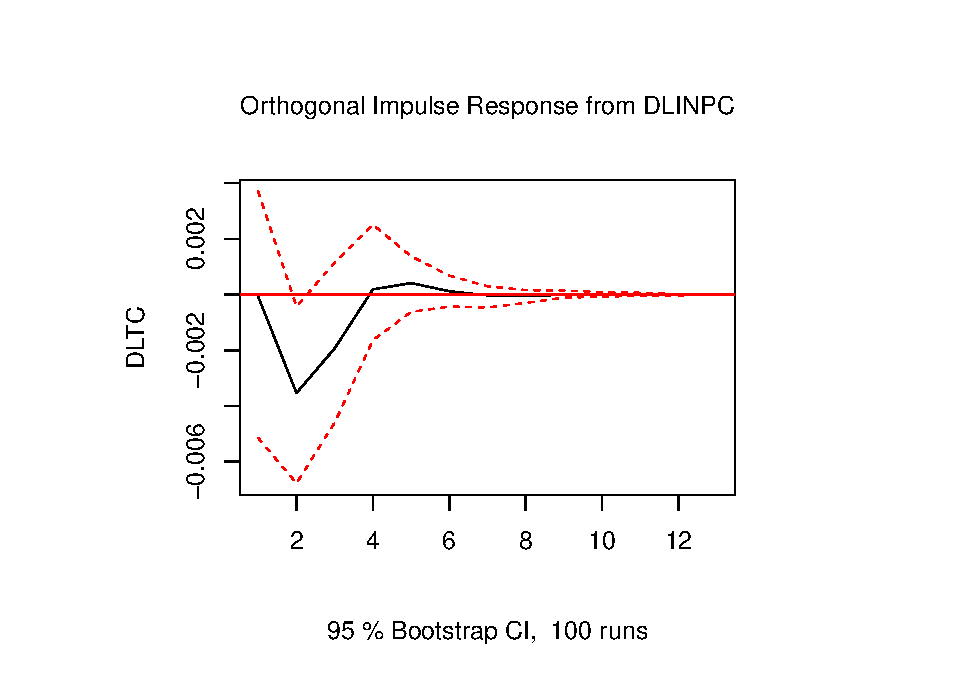
\includegraphics{Notas-Series-Tiempo_files/figure-latex/fig64-1} 

}

\caption{Impulso - Respuesta en $DLTC_t$}\label{fig:fig64-1}
\end{figure}
\begin{figure}

{\centering 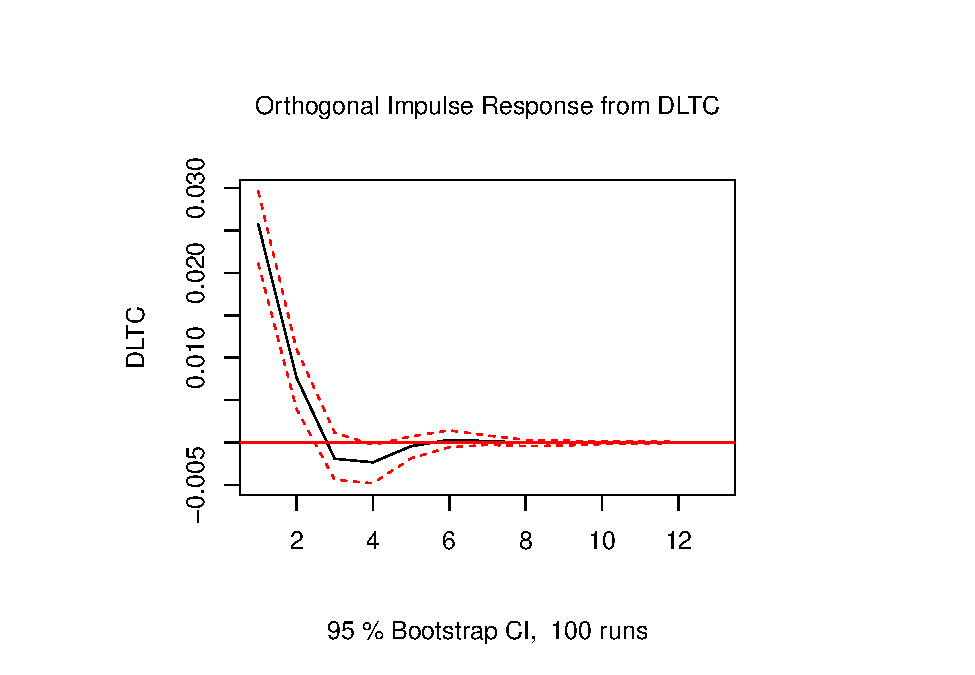
\includegraphics{Notas-Series-Tiempo_files/figure-latex/fig64-2} 

}

\caption{Impulso - Respuesta en $DLTC_t$}\label{fig:fig64-2}
\end{figure}
\begin{figure}

{\centering 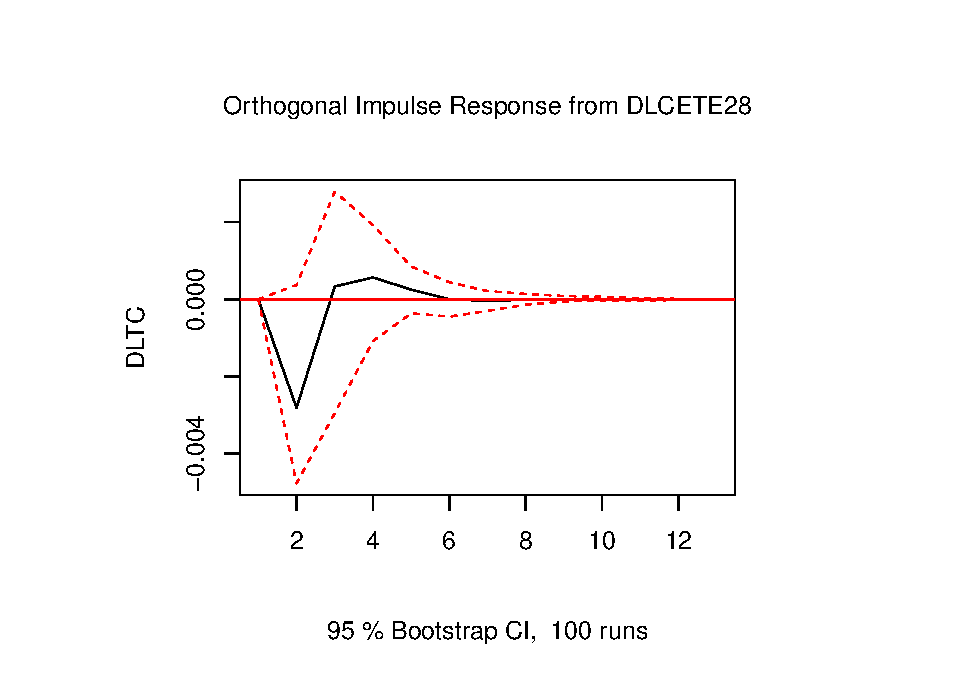
\includegraphics{Notas-Series-Tiempo_files/figure-latex/fig64-3} 

}

\caption{Impulso - Respuesta en $DLTC_t$}\label{fig:fig64-3}
\end{figure}
\begin{figure}

{\centering 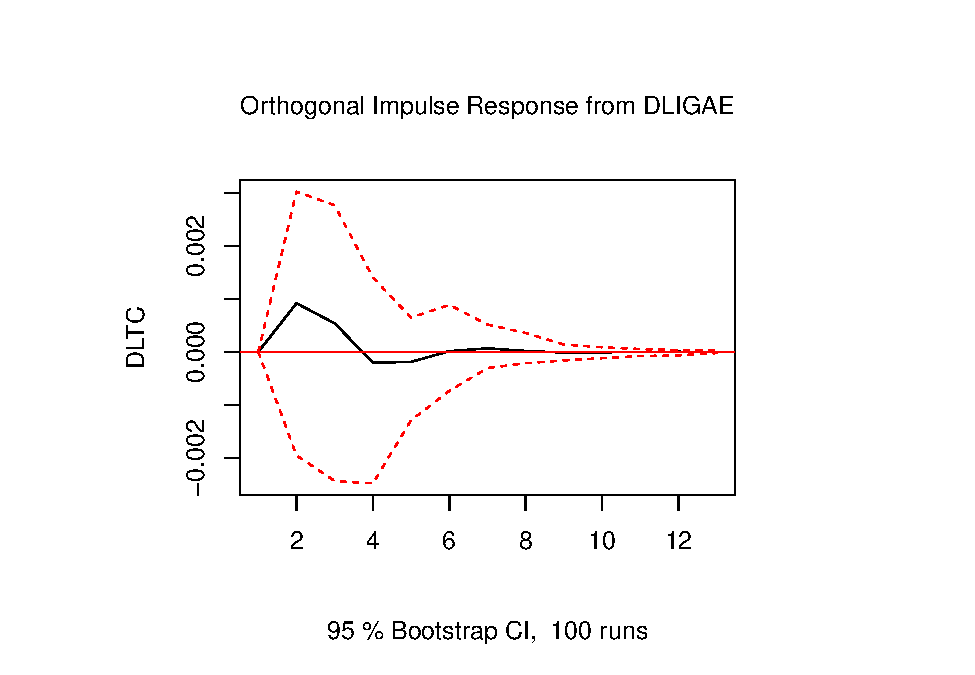
\includegraphics{Notas-Series-Tiempo_files/figure-latex/fig64-4} 

}

\caption{Impulso - Respuesta en $DLTC_t$}\label{fig:fig64-4}
\end{figure}
\begin{figure}

{\centering 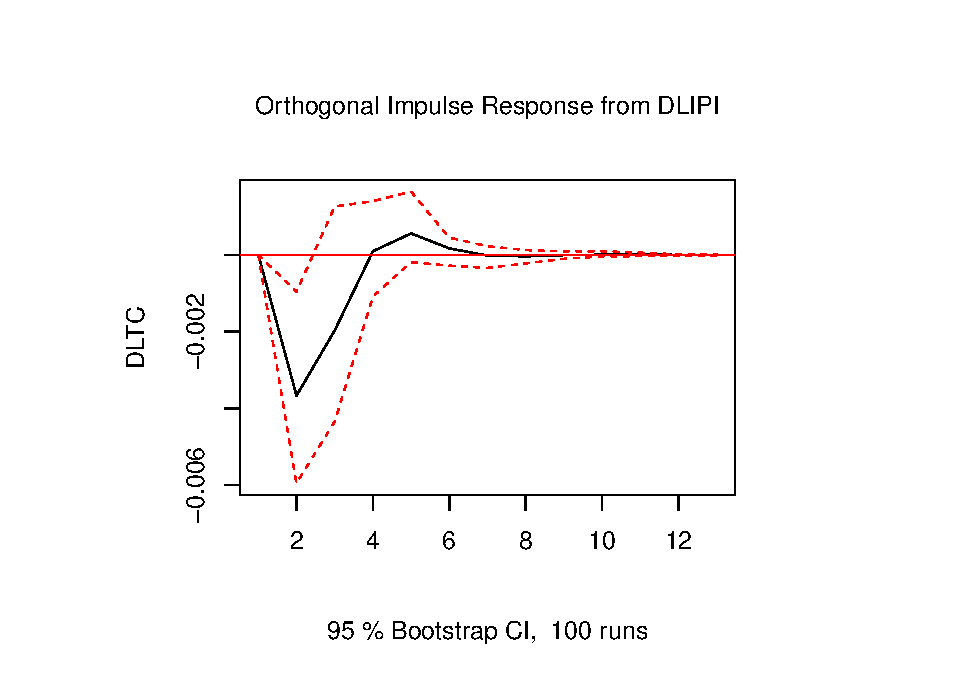
\includegraphics{Notas-Series-Tiempo_files/figure-latex/fig64-5} 

}

\caption{Impulso - Respuesta en $DLTC_t$}\label{fig:fig64-5}
\end{figure}

Los resultados muestran que la respuesta de \(DLTC_t\) ante impulsos en
los términos de error fue estadísticamente significativo sólo para
alguunos de los casos y en periodos cortos de tiempo. El resto de los
resultados de Impulso-Respuesta se encuentra en el Scrip llamado Clase
15 que se ubica en el repositorio de GitHub.

\hypertarget{identificaciuxf3n-de-los-choques-estructurales-en-los-modelos-var}{%
\section{Identificación de los Choques Estructurales en los Modelos VAR}\label{identificaciuxf3n-de-los-choques-estructurales-en-los-modelos-var}}

En su trabajo seminal \emph{``Macroeconomics and Reality''}, Sims (1980)
cuestionó los modelos macroeconométricos utilizados en ese momento.
Antes de la aparición de los modelos de referencia modernos, como los
Vectores Autorregresivos (VAR) y los modelos estocásticos dinámicos de
equilibrio general (DSGE), se estimaban modelos de ecuaciones
simultáneas derivados de la escuela keynesiana, especificados con \(n\) cantidad de ecuaciones. Por lo tanto, para entender el surgimiento de los modelos
VAR en la macroeconometría, es necesario partir del contexto en el que
se escribió el trabajo seminal de Sims.

A finales de los años 70 e inicios de los 80, comenzó una crisis en
torno a los modelos estructurales tradicionales. Los modelos
macroeconómicos de gran escala --como los de la Cowles Commission--
utilizaban restricciones teóricas para identificar relaciones
estructurales que, en muchos casos, eran impuestas de manera arbitraria.
Estos modelos estaban altamente parametrizados y basados en supuestos
teóricos fuertes --como las expectativas adaptativas--, lo que los hacía
sensibles a errores específicos. De esta situación surge en parte la
\emph{Crítica de Lucas}, en la cual Robert Lucas (1976) mostró que este tipo
de modelos fallaba al capturar cambios en el comportamiento cuando las
políticas cambiaban, debido a que no trataban adecuadamente las
expectativas racionales.

Ante este panorama, Sims propuso los modelos VAR, lo que eventualmente
le valió el Premio Nobel de Economía. El objetivo de estos modelos era
ofrecer una alternativa más flexible y empíricamente realista, sin
imponer supuestos estructurales fuertes a priori. De esta manera, los
VAR permiten modelar un conjunto de variables macroeconómicas como
funciones de sus propios rezagos, sin imponer una estructura teórica
rígida. Además, todos los choques y relaciones se tratan inicialmente de
forma simétrica y empírica. Así, los modelos VAR en su forma reducida
son modelos completamente ateóricos.

Sin embargo, aunque los modelos VAR permiten capturar la dinámica
conjunta entre variables sin imponer restricciones teóricas fuertes a
priori, tienen una limitación que no es menor: los choques estimados a
partir de la forma reducida -forma que hemos trabajado hasta
ahora- están correlacionados entre sí. Es decir, los errores \(u_t\)
de la forma reducida reflejan combinaciones lineales de múltiples
choques estructurales y esto nos impide identificar la interacción contemporánea de las variables. Los choques \(u_t\) no se pueden interpretar directamente porque no son ortogonales. En este sentido, para encontrar choques estructurales, debemos encontrar choques \(w_t\) que sí sean ortogonales y tengan una interpretación económica.

Comencemos con la forma estructural del VAR para comprender sus parámetros:
\begin{equation}
B_0 Y_t = B_1 Y_{t-1} + ... B_p Y_{t-p} + w_t
\end{equation}

donde \(w_t\) es un término de error con media cero y no correlacionado en el tiempo, también conocido como innovación estructural o shock estructural. Además, se asume que el término de error es incondicionalmente homocedástico a menos de que se indique lo contrario. La matriz \(B_0\) es no singular y establece la interacción contemporánea entre las variables del modelo. De este modo, el modelo puede escribirse de manera compacta como:
\begin{equation}
B(L) y_t = w_t
\end{equation}

donde \(B(L) \equiv B_0 - B_1 L - B_2 L^2 - ...B_p L^p\) es el polinomio autorregresivo en rezagos. La matriz de covarianza del término de error estructural es normalizada tal que:
\begin{equation}
\mathbb{E}(w_t w_t') \equiv \Sigma_w = I_K.
\end{equation}

Con esto, sabemos que existen tantos shocks estructurales como variables en el modelo. Asimismo, los shocks estructurales, por definición, son mutuamente no correlacionados lo que implica que \(\Sigma_w\) es diagonal. Por último, también sabemos que si normalizamos la varianza de todos los shocks estructurales a uno, no implica una pérdida de generalidad siempre y cuando los elementos diagonales \(B_0\) permanezcan sin restricciones.

Sin embargo, para que el modelo \(B_0 Y_t = B_1 Y_{t-1} + ... B_p Y_{t-p} + w_t\) sea considerado como un VAR estructural no es suficiente con que los elementos de \(w_t\) no se encuentren correlacionados, si no que los choques también deben ser económicamente interpretables. Para esto, derivamos la forma reducida de este modelo VAR estructural de tal modo que \(y_t\) es una función de los rezagos de \(y_t\) únicamente. Si multiplicamos ambos lados de la representación estructural del VAR por \(B_0^{-1}\)
\begin{equation}
B_0^{-1} B_0 y_t = B_0^{-1} B_1 y_{t-1} + ... + B_0^{-1} B_p y_{t-p} + B_0^{-1} w_t
\end{equation}

de tal modo que puede ser representado como
\begin{equation}
y_t = A_1 y_{t-1} + ... + A_p y_{t-p} + u_t 
\end{equation}

donde \(A_i = B_0^{-1} B_i\), \(i = 1,...,p\), y \(u_t = B_0^{-1} w_t\). Asi, las innovaciones en forma reducida de \(u_t\) son un promedio ponderado de los shocks estructurales \(w_t\). De manera compacta, el modelo puede ser expresado como:
\begin{equation}
A(L) y_t = u_t 
\end{equation}

donde \(A(L) = I_K - A_1L - A_2 L^2 - ... A_p L^p\) es el polinomio autorregresivo en rezagos. Los métodos de estimación estándar permiten obtener estimaciones de los parámetros de la forma reducida \(A_i\), para \(i=1,...p\), de las innovaciones reducidas \(u_t\) y de su matriz de covarianza \(\mathbb{E}(u_t u_t') \equiv \Sigma_u\).

Sin embargo, el debate que se ha generado desde entonces es, una vez estimada la forma reducida, de qué manera se puede recuperar la representación estructural del modelo VAR. Es decir, queremos recuperar la matriz \(B_0\) -o bien, su inversa- que contiene las relaciones estructurales contemporáneas de las variables, recordando que \(u_t = B_0^{-1}w_t\).

El método para recuperar dicha matriz ha generado gran debate en el análisis macroeconométrico, dando pie incluso a tesis doctorales al respecto. Con esto en mente, ahora veremos algunos de los métodos clásicos para recuperar las relaciones estructurales de las variables. Nos concentraremos en los siguientes:

\emph{1. Identificación Recursiva}

\emph{2. Restricción de largo plazo}

\emph{3. Imposición de restricciones de signo}

\textbf{\emph{Nota: RStudio es un poco limitado en cuanto a los métodos de identificación de las innovaciones estructurales relacionados con la teoría económica. En realidad, en los trabajos actuales de macroeconometría suele ocuparse, mayoritariamente, el método de Identificación Recursiva. Sin embargo, para ver los métodos de Restricción de largo plazo e Imposición de restricciones de signo, ver el Script de MatLab de estos.}}

\hypertarget{var-recursivo---identificaciuxf3n-recursiva}{%
\subsection{VAR Recursivo - Identificación Recursiva}\label{var-recursivo---identificaciuxf3n-recursiva}}

Una de las formas más populares para recuperar las innovaciones estructurales es mediante la \emph{identificación recursiva}, un caso particular de las restricciones de corto plazo que se implementa utilizando la \textbf{descomposición de Cholesky}.

La idea detrás de este método es simple e intuitivo: queremos recuperar las innovaciones estructurales \(w_t\) a partir de las innovaciones de forma reducida \(u_t\). Para lograr esto, buscamos \emph{ortogonalizar} los errores de forma reducida, lo que en este contexto significa transformarlos en un conjunto de choques no correlacionados contemporáneamente. Es decir, deseamos que \(\mathbb{E}[w_t w_t'] = I\).

Para lograr esto, definimos una matriz \(P\) de tamaño \(K \times K\), triangular inferior y con diagonal principal positiva, de tal modo que:

\begin{equation}
\Sigma_u = \mathbb{E}[u_t u_t'] = P P'
\end{equation}

La matriz \(P\) es conocida como la \textbf{descomposción de Cholesky inferior de \(\Sigma_u\)}. Por ejemplo, en un VAR con tres variables, \(P\) tendría la forma:

\[
P = 
\begin{bmatrix}
p_{11} & 0      & 0 \\
p_{21} & p_{22} & 0 \\
p_{31} & p_{32} & p_{33}
\end{bmatrix}
\]

Ahora, si recordamos que en el modelo estructural los errores están relacionados por \(u_t = B_0^{-1}w_t\) y que

\begin{equation}
\Sigma_u = B_0^{-1} \mathbb{E}[w_t w_t'] B_0^{-1'} = B_0^{-1} B_0^{-1'}
\end{equation}

entonces una solución válida al problema de identificación estructural es asumir que \(B_0^{-1} = P\). Dado que \(P\) es triangular inferior, contiene exactamente \(\frac{K(K-1)}{2}\) ceros impuestos, lo que cumple la condición de orden para identificar todos los elementos libres de la matriz \(B_0^{-1}\). Por simetría. si \(B_0^{-1}\) es triangular inferior, entonces \(B_0\) también lo es -aunque triangular superior-.

Sin embargo, es importante destacar que esta ortogonalización de los errores solo es válida si la estructura recursiva impuesta por la matriz \(P\) se puede justificar con fundamentos económicos. El método impone que la primera variable del sistema responde solo a su propio shock contemporáneo, la segunda puede responder al shock de la primera, la tercera a los dos primeros, y así sucesivamente. Por eso se dice que el modelo estructural resultante es recursivo: se impone una estructura jerárquica de causalidad contemporánea, en lugar de inferirla directamente de los datos.

En este sentido, la \textbf{descomposición de Cholesky} no descubre las relaciones estructurales sino que las impone. Por lo tanto, el orden de las variables en el VAR \textbf{si importa}, ya que determina la interpretación de los shocks estructurales. Por esta razón, se recomienda justificar el orden mediante teoría económica. Por ejemplo, en aplicaciones del Banco de México, el orden se suele establecer de acuerdo con la hipótesis de una economía pequeña y abierta, ordenando las variables de la más exógena a la más endógena.

Veamos un ejemplo rápido de la \emph{identificación recursiva} mediante la \textbf{descomposición de Cholesky}:

\begin{Shaded}
\begin{Highlighting}[]
\CommentTok{\# install.packages("svars")}
\CommentTok{\# install.packages("ggplot2")}
\CommentTok{\# install.packages("ggfortify")}
\FunctionTok{library}\NormalTok{(svars)}
\FunctionTok{library}\NormalTok{(ggplot2)}
\FunctionTok{library}\NormalTok{(ggfortify)}

\NormalTok{var.reducido }\OtherTok{\textless{}{-}}\NormalTok{ vars}\SpecialCharTok{::}\FunctionTok{VAR}\NormalTok{(USA, }\AttributeTok{lag.max =} \DecValTok{10}\NormalTok{, }\AttributeTok{ic =} \StringTok{"AIC"}\NormalTok{)}
\NormalTok{var.estructural }\OtherTok{\textless{}{-}} \FunctionTok{id.chol}\NormalTok{(var.reducido)}
\FunctionTok{summary}\NormalTok{(var.estructural)}
\end{Highlighting}
\end{Shaded}

\begin{verbatim}
## 
## Identification Results
## ---------------------- 
## 
## Method: Cholesky
## Sample size: 169
## 
## Estimated B Matrix (unique decomposition of the covariance matrix): 
##           [,1]      [,2]      [,3]
## x   0.68338360 0.0000000 0.0000000
## pi -0.03642697 1.0726563 0.0000000
## i   0.22450359 0.1818031 0.7672318
\end{verbatim}

\begin{Shaded}
\begin{Highlighting}[]
\CommentTok{\# x  = Porcentaje de desviación logarítmica del PIB real con respecto a la }
\CommentTok{\#      estimación del producto potencial}
\CommentTok{\# pi = Crecimiento anualizado trimestre a trimestre del deflactor del PIB}
\CommentTok{\# i  = Tasa de interés de los fondos federales}

\NormalTok{cores }\OtherTok{\textless{}{-}}\NormalTok{ parallel}\SpecialCharTok{::}\FunctionTok{detectCores}\NormalTok{() }\SpecialCharTok{{-}} \DecValTok{1}
\NormalTok{boot.svar }\OtherTok{\textless{}{-}} \FunctionTok{wild.boot}\NormalTok{(var.estructural, }\AttributeTok{n.ahead =} \DecValTok{24}\NormalTok{, }\AttributeTok{nboot =} \DecValTok{1000}\NormalTok{, }\AttributeTok{nc =}\NormalTok{ cores)}

\FunctionTok{plot}\NormalTok{(boot.svar)}
\end{Highlighting}
\end{Shaded}

\begin{center}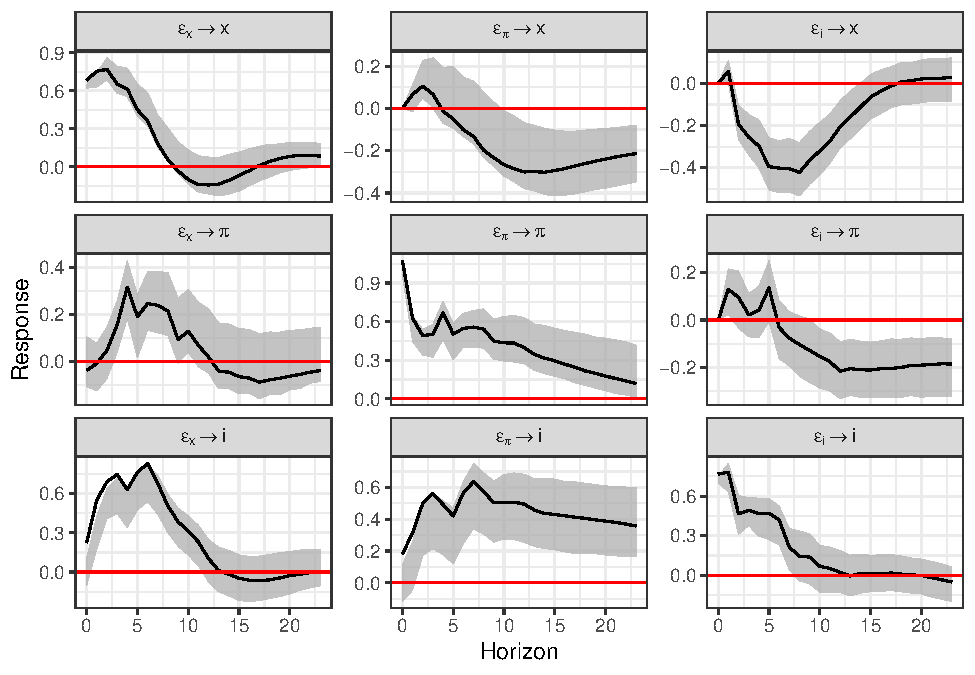
\includegraphics{Notas-Series-Tiempo_files/figure-latex/unnamed-chunk-13-1} \end{center}

\hypertarget{var-estructural---restricciuxf3n-de-largo-plazo}{%
\subsection{VAR Estructural - Restricción de largo plazo}\label{var-estructural---restricciuxf3n-de-largo-plazo}}

Otra manera de identificar las innovaciones estructurales de un modelo VAR, es mediante el método propuesto por Blanchard y Quah (1989) en \emph{``The Dynamic Effects of Aggregate Demand and Supply Disturbances''}.

La intuición de este método es simple: Blanchard y Quah querían medir el efecto de choques de oferta agregada \(w_t^{AS}\) y demanda agregada \(w_t^{AD}\) sobre el Producto y el Desempleo, imponiendo restricciones en la respuesta acumulada, es decir, en el efecto acumulado permanente (horizonte \(h \rightarrow \infty\)). La lógica económica detrás de este método es, básicamente, que el choque de demanda agregada no tiene efectos de largo plazo sobre el nivel del PIB real.

Ahora bien, sean:

\begin{itemize}
\tightlist
\item
  \(ur_t\): tasa de desempleo en EE.UU.
\item
  \(gdp_t\): logaritmo del PIB real de EE.UU.
\end{itemize}

Y definimos el vector \(z_t\)

\begin{equation}
z_t = \begin{bmatrix} \Delta gdp_t \\ ur_t \end{bmatrix} \sim I(0)
\end{equation}

Aunque \(gdp_t \sim I(1)\), su primera diferencia es estacionaria (\(I(0)\)), lo cual justifica que \(z_t \sim I(0)\). Por otro lado, podemos suponer que este vector es generado por un VAR reducido:

\begin{equation}
A(L) z_t = u_t
\end{equation}

donde \(A(L)=I_2-A_1L-...A_pL^p\), y \(u_t \sim (0, \Sigma_u)\) es ruido blanco. Si lo representamos como su forma estructural, tenemos que:

\begin{equation}
B(L) z_t = w_t
\end{equation}

donde \(B(L) = B_0-B_1L-...B_pL^p = B_0A(L)\), y si recordamos a qué es igual \(w_t\), tenemos que:

\begin{equation}
w_t = B_0 u_t \rightarrow u_t = B_0^{-1} w_t \rightarrow \Sigma_u = B_0^{-1} (B_0^{-1})'
\end{equation}

Ahora, pasemos a la representación MA estructural para entender dónde se impone la restricción. Desde el modelo MA, tenemos que:

\begin{equation}
z_t = B(L)^{-1} w_t = \Theta (L) w_t 
\end{equation}

Esto implica que, dado que \(z_t \sim I(0)\), el efecto de un choque estructural sobre \(z_t\) se desvanece con el tiempo y, por tanto, tanto \(\Delta gdp_t\) como \(ur_t\) eventualmente vuelven a su nivel original tras un choque. Sin embargo, el nivel del PIB real -y no su crecimiento- no necesariamente vuelve a su nivel inicial, por lo que la suma acumulada de las respuestas al choque nos da su efecto permanente. Ahora, pasemos a la matriz de efectos acumulados de largo plazo, definida como:

\begin{equation}
\Theta (1) = \sum_{i=0}^{\infty} \Theta_i = B(1)^{-1}
\end{equation}

Dado que queremos que el PIB real vuelva a su tendencia tras un choque de demanda -recordemos que no tiene efectos de largo plazo- implica imponer un cero en la posición \(\theta_{12}\) de la matriz \(\Theta(1)\):

\begin{equation}
\Theta (1) = \begin{bmatrix}
                    \theta_{11} (1) & 0               \\
                    \theta_{21} (1) & \theta_{22} (1)
             \end{bmatrix}
\end{equation}

el hecho de que \(\theta_{12}(1) = 0\) implica que el choque de demanda no afecta permanentemente al PIB real y, por otro lado, que \(\theta_{11}(1)\) permanezca libre, implica que los choques de oferta sí pueden tener efectos de largo plazo.

Para la identificación, recordemos que:

\begin{equation}
\Theta (1) = B(1)^{-1} = A(1)^{-1} B_0^{-1} \rightarrow B_0^{-1} = A(1) \Theta(1)
\end{equation}

De este modo, una vez que conocemos \(A(1)\) y \(\Theta(1)\) podemos recuperar \(B_0^{-1}\), recordando que la restricción en \(\Theta(1)\) es equivalente a imponer una restricción sobre \(B_0\).

Para estimar \(\Theta(1)\), sabemos que:

\begin{equation}
\Sigma_u = B_0^{-1} (B_0^{-1})' = \Theta(1) \Theta(1)'
\end{equation}

y, entonces, si usamos \(A(1)\):

\begin{equation}
A(1)^{-1} \Sigma_u A(1)^{-1'} = \Theta(1) \Theta(1)'
\end{equation}

lo cual implica que podemos calcular el lado izquierdo usando solo parámetros estimados del VAR reducido y luego identificar \(\Theta(1)\) imponiendo que tenga forma triangular inferior, y aplicar la \textbf{descomposición de Cholesky} para tener finalmente que:

\begin{equation}
B_0^{-1} = A(1) \Theta (1)
\end{equation}

\hypertarget{var-estructural---imposiciuxf3n-de-restricciones-de-signo}{%
\subsection{VAR Estructural - Imposición de restricciones de signo}\label{var-estructural---imposiciuxf3n-de-restricciones-de-signo}}

Una alternativa a la identificación de las innovaciones estructurales además de la \emph{Identificación recursiva} es la \textbf{Imposición de restricciones de signo}. Sigue un poco la misma lógica: queremos imponer restricciones de signo en vez de proponer una matriz triangular inferior en la matriz \(B_0^{-1}\). Este método ofrece una alternativa menos restrictiva que imponer ceros exactos. Para explicar este método, tomemos el siguiente modelo ejemplo.

Consideremos un modelo bivariado de un mercado de bienes con:

\begin{itemize}
\tightlist
\item
  Un choque de demanda \(w_t^{demanda}\)
\item
  Un choque de oferta \(w_t^{oferta}\)
\end{itemize}

en donde nuestras variables observables son:

\begin{itemize}
\tightlist
\item
  Precio \(p_t\)
\item
  Cantidad \(q_t\)
\end{itemize}

Y los errores en forma reducida están dados por:

\begin{equation}
u_t = \begin{bmatrix} u_t^q \\ u_t^p \end{bmatrix} = B_0^{-1} w_t 
      \quad \text{donde} \quad 
w_t = \begin{bmatrix} w_t^{oferta} \\ w_t^{demanda} \end{bmatrix}
\end{equation}

Es sencillo: la interpretación económica es que los efectos de los choques \(u_t\) dependen de la pendiente de las curvas de demanda y oferta.

En un método tradicional -restricción de exclusión-, se asume que la oferta es vertical en el corto plazo, lo cual implica que los choques de demanda no afectan la cantidad contemporáneamente:

\begin{equation}
\begin{bmatrix} u_t^q \\ u_t^p \end{bmatrix} = 
\begin{bmatrix} \ast & 0 \\
                \ast & \ast 
                \end{bmatrix}
\begin{bmatrix} w_t^{oferta} \\ w_t^{demanda} \end{bmatrix}
\end{equation}

En donde los asteriscos representan \emph{coeficientes libres} y el cero es una \emph{restricción de exclusión}.

En cambio, si tomamos la teoría económica básica en el enfoque alternativo de \textbf{Imposición de restricción de signo} esperaríamos que, ante un choque de oferta positivo -la curva de oferta se desplaza a la derecha-, la cantidad aumente y el precio caiga, mientras que, ante un choque de demanda positiva -la curva de demanda se desplaza a la derecha-, la cantidad aumenta y el precio aumenta. De este modo, tenemos que:

\begin{equation}
  \begin{bmatrix} u_t^q \\ u_t^p \end{bmatrix} = 
    \underbrace{
  \begin{bmatrix} + & + \\ - & + \end{bmatrix}
    }_{B_0^{-1}}
  \begin{bmatrix} w_t^{\text{oferta}} \\ w_t^{\text{demanda}} \end{bmatrix}
\end{equation}

Donde \(+\) indica signo positivo estricto y \(-\) negativo estricto.

La diferencia clave con el método de \emph{Identificación recursiva mediante la descomposición de Cholesky} es que, en estos últimos modelos, los parámetros están puntualmente identificados mientras que con \textbf{restricciones de signo} los parámetros no se identifican exactamente, sino que quedan dentro de un conjunto compatible con las restricciones. De este modo, no hay una única solución, pues hay muchas matrices \(B_0^{-1}\) que cumplen con los signos impuestos. También, se pueden imponer \textbf{restricciones de signo} de la siguiente forma:

\begin{equation}
  \begin{bmatrix} + & + \\ 0 & + \end{bmatrix}
      \quad \text{o} \quad 
  \begin{bmatrix} + & + \\ - & 0 \end{bmatrix}
\end{equation}

Estas formas también pueden ser admisibles pero algunas podrían llegar a ser problemáticas si llevan a choques no identificables entre sí.

Se dice que los modelos identificados por signos son más generales que los recursivos pero no son modelos ``anidados'', o sea, uno no puede validar o rechazar el otro con datos. Así, las \textbf{restricciones de signo} permiten más flexibilidad, pero imponen otras limitaciones como perder identificación puntual.

Ahora, de manera más puntual, para imponer las \textbf{restricciones de signo estáticas} consideremos un modelo VAR en su forma estructural:

\begin{equation}
B_0 y_t = B_1 y_{t-1} + ... + B_p y_{t-p} + w_t
\end{equation}

y normalizamos la matriz de varianzas-covarianzas del término de error estructural \(w_t\) tal que:

\begin{equation}
\mathbb{E}(w_t w_t') \equiv \Sigma_w = I_K.
\end{equation}

Ahora, sea \(u_t = P \eta_t\), donde \(u_t\) es la innovación del VAR en forma reducida y \(P\) es la descomposición de Cholesky de \(\Sigma_u\). Por construcción, los choques \(\eta_t\) son mutuamente no correlacionados y tienen varianza unitaria. Por supuesto, no hay razón para que estos choques correspondan a choques estructurales económicamente interpretables, como los choques de oferta y demanda en el modelo bivariado mencionado anteriormente. Sin embargo, podemos buscar soluciones candidatas \(w_t^*\) para los choques estructurales desconocidos \(w_t\) construyendo un gran número de combinaciones de los choques \(\eta_t\) de la forma:

\begin{equation}
w_t^* = Q' \eta_t, 
\end{equation}

donde \(Q'\) es una matriz ortogonal cuadrada tal que \(Q'Q = QQ' = I_K\) y \(u_t = PQ \eta_t = PQw_t^*\). Por lo tanto, cada solución candidata \(w_t^*\) consiste en choques no correlacionados con varianza unitaria. Que una de estas soluciones candidatas \(w_t^*\) sea una solución admisible para el choque estructural desconocido \(w_t\), dado el vector de parámetros en forma reducida, depende de si la matriz de impacto estructural implicado \(PQ\) satisface las restricciones de signo mantenidas sobre \(B_0^{-1}\). De este modo, solo conservamos las soluciones que satisfagan las restricciones de signo y se descartan las demás. El hecho de repetir este procedimiento nos permite caracterizar el conjunto de todos los modelos estructurales que son consistentes con las restricciones de signo mantenidas y los parámetros en forma reducida. Conocer \(PQ\) permite construir todos los coeficientes estructurales de respuesta al impulso que se derivan de las estimaciones de los parámetros en forma reducida.

Los dos enfoques comunes para construir las matrices ortogonales \(Q\) están basados en:

\begin{enumerate}
\def\labelenumi{\arabic{enumi}.}
\item
  Matrices de rotación de Givens.
\item
  Transformación de Householder.
\end{enumerate}

La paquetería del código de MatLab, VAR Toolbox, ocupa el enfoque de \textbf{Matrices de rotación de Givens}.

\hypertarget{cointegraciuxf3n}{%
\section{Cointegración}\label{cointegraciuxf3n}}

Hasta ahora en el curso hemos usado el supuesto de que las series son
estacionarias para el conjunto de técnicas \(ARMA(p,q)\) y \(VAR(p)\). No
obstante, dado que relajamos el supuesto de estacionariedad (incluyendo
la estacionariedad en varianza) y que establecimos una serie de pruebas
para determinar cuándo una serie es estadísticamente estacionaria, ahora
podemos plantear una técnica llamada Cointegración. Para esta técnica
consideraremos sólo series que son \(I(1)\) y reconoceremos que se originó
con los trabajos de Engle y Granger (1987), Stock (1987) y Johansen
(1988).

\hypertarget{definiciuxf3n-y-propiedades-del-proceso-de-cointegraciuxf3n}{%
\subsection{Definición y propiedades del proceso de cointegración}\label{definiciuxf3n-y-propiedades-del-proceso-de-cointegraciuxf3n}}

Cointegración puede ser caracterizada o definida en palabras sencillas
como que dos o más variables tienen una relación común estable en el
largo plazo. Es decir, estas no suelen tomar caminos o trayectorias
diferentes, excepto por períodos de tiempo transitorios y eventuales. A
continuación, utilizaremos la definición de Engle y Granger (1984) de
cointegración.

Sea \(\mathbf{Y}\) un vector de k-series de tiempo, decimos que los
elementos en \(\mathbf{Y}\) están cointegrados en un orden (d, c), es
decir, \(\mathbf{Y} \sim CI(d, c)\), si todos los elementos de
\(\mathbf{Y}\) son series integradas de orden d, I(d), y si existe al
menos una combinación lineal no trivial \(\mathbf{Z}\) de esas variables
que es de orden I(d - c), donde \(d \geq c > 0\), si y sólo si:
\begin{equation}
    \boldsymbol{\beta}_i' \mathbf{Y}_t = \mathbf{Y}_{it} \sim I(d-c)
\end{equation}

Donde \(i = 1, 2, \ldots, r\) y \(r < k\).

A los diferentes vectores \(\boldsymbol{\beta}_i\) se les denomina como
vectores de cointegración. El rango de la matriz de vectores de
cointegración \(r\) es el número de vectores de cointegración linealmente
independientes. En general diremos que los vectores de la matriz de
cointegración \(\boldsymbol{\beta}\) tendrán la forma de: \begin{equation}
    \boldsymbol{\beta}' \mathbf{Y}_t = \mathbf{Z}_t
\end{equation}

Antes de continuar hagamos algunas observaciones. Si todas las variables
de \(\mathbf{Y}\) son I(1) y \(0 \leq r < k\), diremos que las series no
cointegran si \(r = 0\). Si esto pasa, entonces, como demostraremos más
adelante, la mejor opción será estimar un modelo VAR(p) en diferencias.
Adicionalmente, asumiremos que \(c = d = 1\), por lo que la relación de
cointegración, en su caso, generará combinaciones lineales \(\mathbf{Z}\)
estacionarias.

\hypertarget{cointegraciuxf3n-para-modelos-de-muxe1s-de-una-ecuaciuxf3n-o-para-modelos-basados-en-vectores-autoregresivos}{%
\subsection{Cointegración para modelos de más de una ecuación o para modelos basados en Vectores Autoregresivos}\label{cointegraciuxf3n-para-modelos-de-muxe1s-de-una-ecuaciuxf3n-o-para-modelos-basados-en-vectores-autoregresivos}}

Sean \(Y_1, Y_2, \ldots, Y_k\) son series que forman \(\mathbf{Y}\) y que
todas son I(1), entonces los siguientes casos son posibles:

\begin{enumerate}
\def\labelenumi{\arabic{enumi}.}
\item
  Si \(r = 1\) entonces se trata de un caso de cointegración de Granger.
\item
  Si \(r \geq 1\) entonces se trata de un caso de cointegración múltiple
  de Johansen.
\end{enumerate}

Por lo anterior, en este curso analizaremos el caso de Cointegración de
Johansen. Ahora plantearemos la forma de estimar el proceso de
cointegración. El primer paso para ello es determinar un modelo VAR(p)
con las k-series no estacionarias (series en niveles)--en este punto se
vuelve fundamental caracterizar las series a través de pruebas de raíces
unitarias--. Elegimos el valor de \(p\) mediante el uso de los criterios
de información. De esta forma tendremos una especificación similar a:
\begin{equation}
    \mathbf{Y}_t = \sum_{j=1}^p \mathbf{A}_j \mathbf{Y}_{t-j} + \mathbf{D}_t + \mathbf{U}_t
    \label{eq:VARCI}
\end{equation}

Donde \(\mathbf{U}_t\) es un término de error k-dimensional puramente
aleatorio; \(\mathbf{D}_t\) contiene los componentes determinísticos de
constante y tendencia, y \(\mathbf{A}_i\), \(i = 1, 2, \ldots, p\), son
matrices de \(k \times k\) coeficientes. Notemos que el VAR(p) involucrado
en este caso, a diferencia del VAR anteriormente estudiado, puede
incluir un término de tendencia. Esto en razón de que hemos relajado el
concepto de estacionariedad.

Si reescribimos la ecuación \eqref{eq:VARCI} en su forma de Vector
Corrector de Errores (VEC, por sus siglas en inglés) tenemos:
\begin{eqnarray}
    \mathbf{Y}_t - \mathbf{Y}_{t-1} & = & \Delta \mathbf{Y}_t \nonumber \\
    & = & \sum_{j=1}^p \mathbf{A}_j \mathbf{Y}_{t-j} + \mathbf{D}_t - \mathbf{Y}_{t-1} + \mathbf{U}_t \nonumber \\
    & = & (\mathbf{A}_1 - \mathbf{I}) \mathbf{Y}_{t-1} + \mathbf{A}_2 \mathbf{Y}_{t-2} + \ldots + \mathbf{A}_p \mathbf{Y}_{t-p} + \mathbf{D}_t + \mathbf{U}_t \nonumber \\
    & = & \left( \sum_{j=1}^{p} \mathbf{A}_j - \mathbf{I} \right) \mathbf{Y}_{t-1} + \sum_{j=1}^{p-1} \mathbf{A}^*_j \Delta \mathbf{Y}_{t-j} + \mathbf{D}_t \mathbf{U}_t \nonumber \\
    & = & - \left( \mathbf{I} - \sum_{j=1}^{p} \mathbf{A}_j \right) \mathbf{Y}_{t-1} + \sum_{j=1}^{p-1} \mathbf{A}^*_j \Delta \mathbf{Y}_{t-j} + \mathbf{D}_t \mathbf{U}_t \nonumber \\
    \Delta \mathbf{Y}_t & = & - \Pi \mathbf{Y}_{t-1} + \sum_{j=1}^{p-1} \mathbf{A}^*_j \Delta \mathbf{Y}_{t-j} + \mathbf{D}_t + \mathbf{U}_t
    \label{eq:VARVEC}
\end{eqnarray}

Donde \(\mathbf{A}_j^* = - \sum_{i=j+1}^p \mathbf{A}_i\),
\(i = 1, 2, \ldots, p-1\), y la matriz \(\Pi\) representa todas las
relaciones de largo plazo entre las variables, por lo que la matriz es
de rango completo \(k \times k\). Por lo tanto, tenemos que dicha matriz
en la ecuación \eqref{eq:VARVEC} se puede factorizar como:
\begin{equation}
    \Pi_{(k \times k)} = \Gamma_{(k \times r)} \boldsymbol{\beta}_{(r \times k)}'
    (\#eq:Pi_Matrix)
\end{equation}

Donde \(\boldsymbol{\beta}_{(r \times k)}' \mathbf{Y}_{t-1}\) son \(r\)
combinaciones linealmente independientes que son estacionarias.

Dada la ecuación \eqref{eq:VARVEC} podemos establecer la aproximación de
Johansen (1988) que se realiza mediante una estimación por Máxima
Verosimilitud de la ecuación: \begin{equation}
    \Delta \mathbf{Y}_t + \Gamma \boldsymbol{\beta}' \mathbf{Y}_{t-1} = \sum_{j=1}^{p-1} \mathbf{A}^*_j \Delta \mathbf{Y}_{t-j} + \mathbf{D}_t + \mathbf{U}_t
\end{equation}

Donde una vez estimado el sistema: \begin{equation}
    \boldsymbol{\beta} = [v_1, v_2, \ldots, v_r]
\end{equation}

Cada \(v_i\), \(i = 1, 2, \ldots, r\) es un vector propio que está asociado
con los \(r\) valores propios positivos, mismos que están asociados con la
prueba de hipótesis de cointegración. Dicha hipótesis está basada en dos
estadísticas con las que se determina el rango \(r\) de \(\Pi\):

\begin{enumerate}
\def\labelenumi{\arabic{enumi}.}
\item
  Prueba de Traza: \(H_0 :\) Existen al menos \(r\) valores propios
  positivos o Existen al menos \(r\) relaciones de largo plazo
  estacionarias.
\item
  Prueba del valor propio máximo o \(\lambda_{max}\): \(H_0 :\) Existen
  \(r\) valores propios positivos o Existen \(r\) relaciones de largo
  plazo estacionarias.
\end{enumerate}

\textbf{Ejemplo}. Para ejemplificar el procedimiento de cointegración
utilizaremos las series de INPC, Tipo de Cambio, rendimiento de los
Cetes a 28 días, IGAE e Índice de Producción Industrial de Estados
Unidos. Quizá el marco teórico de la relación entre las variables no sea
del todo correcto, pero dejando de lado ese problema, estimaremos si las
5 series cointegran.

Por principio, probaremos que todas las series son I(1), lo cual es
cierto (ver Scrip para mayores detalles). En las Figuras
\ref{fig:fig81}, \ref{fig:fig82} y \ref{fig:fig83} se muestran las
series en niveles y en diferencias, con lo cual ilustramos como es
viable que las series sean I(1).

\begin{Shaded}
\begin{Highlighting}[]
\FunctionTok{library}\NormalTok{(ggplot2)}
\FunctionTok{library}\NormalTok{(dplyr)}
\FunctionTok{library}\NormalTok{(stats)}
\FunctionTok{library}\NormalTok{(MASS)}
\FunctionTok{library}\NormalTok{(strucchange)}
\FunctionTok{library}\NormalTok{(zoo)}
\FunctionTok{library}\NormalTok{(sandwich)}
\FunctionTok{library}\NormalTok{(urca)}
\FunctionTok{library}\NormalTok{(lmtest)}
\FunctionTok{library}\NormalTok{(vars)}

\CommentTok{\#}
\FunctionTok{load}\NormalTok{(}\StringTok{"BD/Datos\_Ad.RData"}\NormalTok{)}

\CommentTok{\#}
\DocumentationTok{\#\# Conversion a series de tiempo:}
\NormalTok{Datos }\OtherTok{\textless{}{-}} \FunctionTok{ts}\NormalTok{(Datos\_Ad[}\DecValTok{7}\SpecialCharTok{:} \DecValTok{11}\NormalTok{], }
            \AttributeTok{start =} \FunctionTok{c}\NormalTok{(}\DecValTok{2000}\NormalTok{, }\DecValTok{1}\NormalTok{), }
            \AttributeTok{freq =} \DecValTok{12}\NormalTok{)}

\NormalTok{LDatos }\OtherTok{\textless{}{-}} \FunctionTok{log}\NormalTok{(Datos)}

\NormalTok{DLDatos }\OtherTok{\textless{}{-}} \FunctionTok{diff}\NormalTok{(}\FunctionTok{log}\NormalTok{(Datos, }\AttributeTok{base =} \FunctionTok{exp}\NormalTok{(}\DecValTok{1}\NormalTok{)), }
                \AttributeTok{lag =} \DecValTok{1}\NormalTok{, }
                \AttributeTok{differences =} \DecValTok{1}\NormalTok{)}
\end{Highlighting}
\end{Shaded}

\begin{Shaded}
\begin{Highlighting}[]
\FunctionTok{plot}\NormalTok{(LDatos, }
     \AttributeTok{plot.type =} \StringTok{"m"}\NormalTok{, }\AttributeTok{nc =} \DecValTok{2}\NormalTok{,}
     \AttributeTok{col =} \FunctionTok{c}\NormalTok{(}\StringTok{"darkgreen"}\NormalTok{, }\StringTok{"darkblue"}\NormalTok{, }\StringTok{"darkred"}\NormalTok{, }\StringTok{"orange"}\NormalTok{, }\StringTok{"purple"}\NormalTok{), }
     \CommentTok{\#main = "Series en Logaritmos", }
     \AttributeTok{xlab =} \StringTok{"Tiempo"}\NormalTok{)}
\end{Highlighting}
\end{Shaded}

\begin{figure}

{\centering 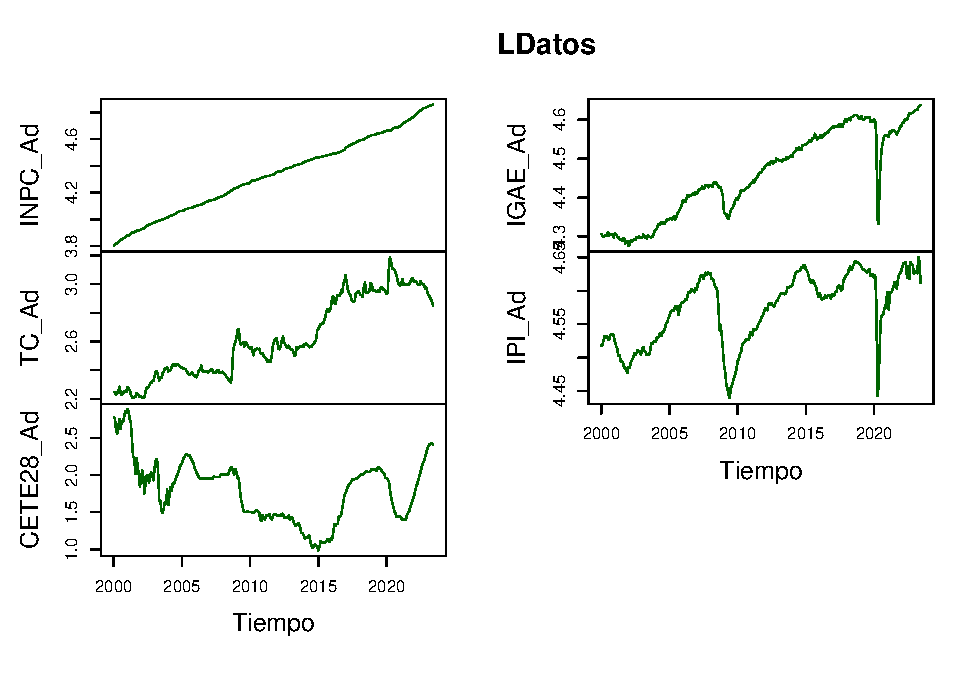
\includegraphics{Notas-Series-Tiempo_files/figure-latex/fig81-1} 

}

\caption{Series en niveles (logaritmos) para la prueba de Cointegración}\label{fig:fig81}
\end{figure}

\begin{Shaded}
\begin{Highlighting}[]
\FunctionTok{plot}\NormalTok{(DLDatos, }
     \AttributeTok{plot.type =} \StringTok{"m"}\NormalTok{, }\AttributeTok{nc =} \DecValTok{2}\NormalTok{,}
     \AttributeTok{col =} \FunctionTok{c}\NormalTok{(}\StringTok{"darkgreen"}\NormalTok{, }\StringTok{"darkblue"}\NormalTok{, }\StringTok{"darkred"}\NormalTok{, }\StringTok{"orange"}\NormalTok{, }\StringTok{"purple"}\NormalTok{), }
     \CommentTok{\#main = "Series en Diferencias Logaritmicas", }
     \AttributeTok{xlab =} \StringTok{"Tiempo"}\NormalTok{)}
\end{Highlighting}
\end{Shaded}

\begin{figure}

{\centering 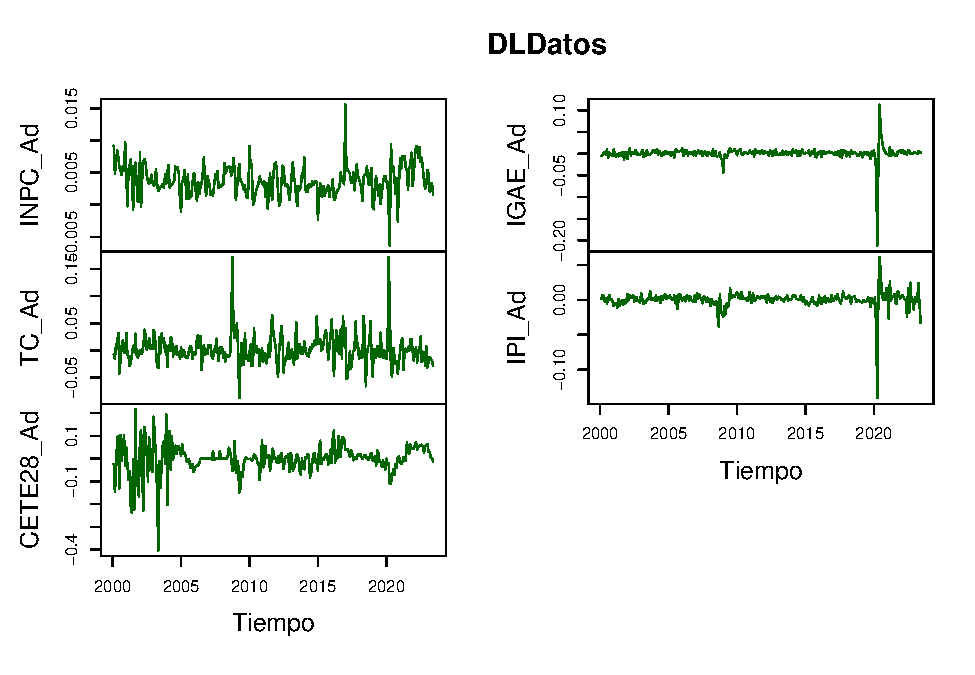
\includegraphics{Notas-Series-Tiempo_files/figure-latex/fig82-1} 

}

\caption{Series en Diferencias Logarítmicas para la prueba de Cointegración}\label{fig:fig82}
\end{figure}

\begin{Shaded}
\begin{Highlighting}[]
\FunctionTok{plot}\NormalTok{(}\FunctionTok{cbind}\NormalTok{(LDatos, DLDatos), }
     \AttributeTok{plot.type =} \StringTok{"m"}\NormalTok{, }\AttributeTok{nc =} \DecValTok{2}\NormalTok{,}
     \AttributeTok{col =} \FunctionTok{c}\NormalTok{(}\StringTok{"darkgreen"}\NormalTok{, }\StringTok{"darkblue"}\NormalTok{, }\StringTok{"darkred"}\NormalTok{, }\StringTok{"orange"}\NormalTok{, }\StringTok{"purple"}\NormalTok{), }
     \CommentTok{\#main = "Comparacion de Series en Diferencias", }
     \AttributeTok{xlab =} \StringTok{"Tiempo"}\NormalTok{)}
\end{Highlighting}
\end{Shaded}

\begin{figure}

{\centering 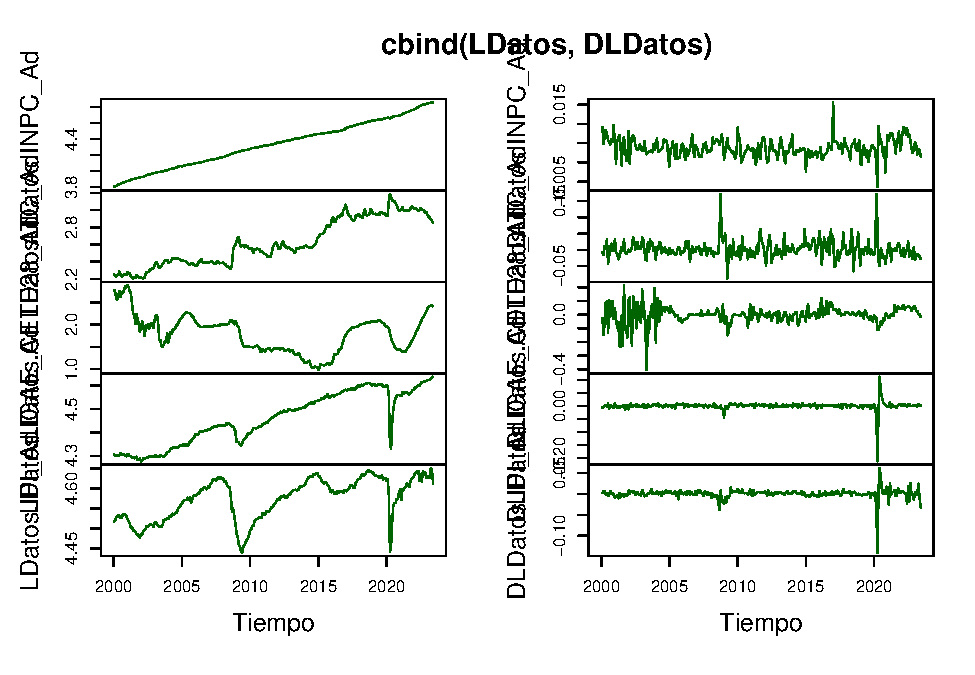
\includegraphics{Notas-Series-Tiempo_files/figure-latex/fig83-1} 

}

\caption{Comparacion de Series en Diferencias para la prueba de Cointegración}\label{fig:fig83}
\end{figure}

Posteriormente, determinamos cuál es el orden adecuado de un VAR(p) en
niveles. En el Cuadro \ref{tab:SelectVARVEC} mostramos los resultados
de los criterios de información para determinar el número de rezagos
óptimos, el cual resultó en \(p = 3\) para los criterios AIC y FPE,
\(p = 2\) para el criterio HQ y \(p = 1\) para el criterio SC. Por lo tanto,
decidiremos utilizar un VAR(3) con tendencia y constante. Note que es
posible elegir otros modelos de VAR que incluyan: solo tendencia, solo
constante o ninguno de estos elementos.

\begin{longtable}[]{@{}
  >{\centering\arraybackslash}p{(\columnwidth - 8\tabcolsep) * \real{0.1324}}
  >{\centering\arraybackslash}p{(\columnwidth - 8\tabcolsep) * \real{0.2206}}
  >{\centering\arraybackslash}p{(\columnwidth - 8\tabcolsep) * \real{0.2206}}
  >{\centering\arraybackslash}p{(\columnwidth - 8\tabcolsep) * \real{0.2206}}
  >{\centering\arraybackslash}p{(\columnwidth - 8\tabcolsep) * \real{0.2059}}@{}}
\caption{\label{tab:SelectVARVEC} Criterios de información para diferentes
especificaciones de modelos VAR(p) con término constante y tendencia de
las series \(LINPC_t\), \(LTC_t\), \(LCETE28_t\), \(LIGAE_t\) y \(LIPI_t\).}\tabularnewline
\toprule\noalign{}
\begin{minipage}[b]{\linewidth}\centering
Rezagos
\end{minipage} & \begin{minipage}[b]{\linewidth}\centering
AIC
\end{minipage} & \begin{minipage}[b]{\linewidth}\centering
HQ
\end{minipage} & \begin{minipage}[b]{\linewidth}\centering
SC
\end{minipage} & \begin{minipage}[b]{\linewidth}\centering
FPE
\end{minipage} \\
\midrule\noalign{}
\endfirsthead
\toprule\noalign{}
\begin{minipage}[b]{\linewidth}\centering
Rezagos
\end{minipage} & \begin{minipage}[b]{\linewidth}\centering
AIC
\end{minipage} & \begin{minipage}[b]{\linewidth}\centering
HQ
\end{minipage} & \begin{minipage}[b]{\linewidth}\centering
SC
\end{minipage} & \begin{minipage}[b]{\linewidth}\centering
FPE
\end{minipage} \\
\midrule\noalign{}
\endhead
\bottomrule\noalign{}
\endlastfoot
1 & -4.606707e+01 & -4.585260e+01 & -4.553568e+01 & 9.848467e-21 \\
2 & -4.643287e+01 & -4.606521e+01 & -4.552191e+01 & 6.834064e-21 \\
3 & -4.647783e+01 & -4.595697e+01 & -4.518730e+01 & 6.539757e-21 \\
4 & -4.645834e+01 & -4.578428e+01 & -4.478824e+01 & 6.679778e-21 \\
\vdots & \vdots & \vdots & \vdots & \vdots \\
\end{longtable}

\begin{Shaded}
\begin{Highlighting}[]
\DocumentationTok{\#\# VAR(p) Seleccion:}

\FunctionTok{VARselect}\NormalTok{(LDatos, }\AttributeTok{lag.max =} \DecValTok{10}\NormalTok{, }\AttributeTok{type =} \StringTok{"both"}\NormalTok{)}
\end{Highlighting}
\end{Shaded}

\begin{verbatim}
## $selection
## AIC(n)  HQ(n)  SC(n) FPE(n) 
##      3      2      2      3 
## 
## $criteria
##                                    1                             2
## AIC(n) -43.1308318646810135987834656 -43.5668661854371990216350241
## HQ(n)  -42.9445592539269327403417265 -43.2475417098587726627556549
## SC(n)  -42.6668499811502783813921269 -42.7714686708130784609238617
## FPE(n)   0.0000000000000000001855848   0.0000000000000000001200259
##                                    3                             4
## AIC(n) -43.5797269785975984746073664 -43.5035550099222803055454278
## HQ(n)  -43.1273506381948337207177246 -42.9181268046951771566455136
## SC(n)  -42.4529138328800996760037378 -42.0453262331114032690493332
## FPE(n)   0.0000000000000000001185548   0.0000000000000000001280605
##                                    5                             6
## AIC(n) -43.4665644031667497415583057 -43.3662074624718840709647338
## HQ(n)  -42.7480843331153010922207613 -42.5146755275960970266169170
## SC(n)  -41.6769199952624873617423873 -41.2451474234742434532563493
## FPE(n)   0.0000000000000000001330869   0.0000000000000000001474594
##                                    7                             8
## AIC(n) -43.3576732552204475723556243 -43.4475783817780367712657608
## HQ(n)  -42.3730894555203079221428197 -42.3299427172535587260426837
## SC(n)  -40.9051975851294216113274160 -40.6636870805936325723450864
## FPE(n)   0.0000000000000000001491718   0.0000000000000000001368875
##                                    9                            10
## AIC(n) -43.3742641642367701138027769 -43.3660356138277762738653109
## HQ(n)  -42.1235766348879465681420697 -41.9822962196546143331943313
## SC(n)  -40.2589572319589734661349212 -39.9193130504566013883049891
## FPE(n)   0.0000000000000000001480478   0.0000000000000000001502148
\end{verbatim}

\begin{Shaded}
\begin{Highlighting}[]
\FunctionTok{VARselect}\NormalTok{(LDatos, }\AttributeTok{lag.max =} \DecValTok{10}\NormalTok{, }\AttributeTok{type =} \StringTok{"trend"}\NormalTok{)}
\end{Highlighting}
\end{Shaded}

\begin{verbatim}
## $selection
## AIC(n)  HQ(n)  SC(n) FPE(n) 
##      3      2      2      3 
## 
## $criteria
##                                    1                             2
## AIC(n) -43.0218334558386885646541486 -43.4733608627676417768270767
## HQ(n)  -42.8621712180494753852144640 -43.1806467601540902023771196
## SC(n)  -42.6241346985266318370122463 -42.7442464743621997058653506
## FPE(n)   0.0000000000000000002069525   0.0000000000000000001317817
##                                    3                             4
## AIC(n) -43.4926570116813877575623337 -43.4403901004477006608794909
## HQ(n)  -43.0668910442434906826747465 -42.8815722681854651909816312
## SC(n)  -42.4321269921825603432807839 -42.0484444498554950087054749
## FPE(n)   0.0000000000000000001293226   0.0000000000000000001363788
##                                    5                             6
## AIC(n) -43.4055918510038054591859691 -43.3210122680509144288407697
## HQ(n)  -42.7137221539172173834231216 -42.4960907061399879580676497
## SC(n)  -41.6822305693182144636921294 -41.2662353552719451954544638
## FPE(n)   0.0000000000000000001414042   0.0000000000000000001541996
##                                    7                             8
## AIC(n) -43.3018930975745490741246613 -43.3631837990786621617189667
## HQ(n)  -42.3439196708392771029139112 -42.2721585075190517954979441
## SC(n)  -40.9157005537021944974185317 -40.6455756241129293471203709
## FPE(n)   0.0000000000000000001576227   0.0000000000000000001488111
##                                    9                           10
## AIC(n) -43.3123078988938914335449226 -43.289311818269602838427090
## HQ(n)  -42.0882307425099355668862700 -41.932182797061308576758165
## SC(n)  -40.2632840928347732756265032 -39.908872381117106442616205
## FPE(n)   0.0000000000000000001573361   0.000000000000000000161972
\end{verbatim}

\begin{Shaded}
\begin{Highlighting}[]
\FunctionTok{VARselect}\NormalTok{(LDatos, }\AttributeTok{lag.max =} \DecValTok{10}\NormalTok{, }\AttributeTok{type =} \StringTok{"const"}\NormalTok{)}
\end{Highlighting}
\end{Shaded}

\begin{verbatim}
## $selection
## AIC(n)  HQ(n)  SC(n) FPE(n) 
##      3      2      2      3 
## 
## $criteria
##                                    1                            2
## AIC(n) -43.0529318587713945021278050 -43.495191294123372927060700
## HQ(n)  -42.8932696209821813226881204 -43.202477191509821352610743
## SC(n)  -42.6552331014593377744859026 -42.766076905717930856098974
## FPE(n)   0.0000000000000000002006156   0.000000000000000000128936
##                                    3                             4
## AIC(n) -43.5086218228659333817631705 -43.4510965812944505159975961
## HQ(n)  -43.0828558554280363068755833 -42.8922787490322150460997364
## SC(n)  -42.4480918033671059674816206 -42.0591509307022448638235801
## FPE(n)   0.0000000000000000001272744   0.0000000000000000001349265
##                                    5                            6
## AIC(n) -43.4144752420798099024068506 -43.325553474358613925687678
## HQ(n)  -42.7226055449932289320713608 -42.500631912447687454914558
## SC(n)  -41.6911139603942189069130109 -41.270776561579644692301372
## FPE(n)   0.0000000000000000001401536   0.000000000000000000153501
##                                    7                             8
## AIC(n) -43.3069657328556019137977273 -43.3724989978216228792007314
## HQ(n)  -42.3489923061203299425869773 -42.2814737062620125129797088
## SC(n)  -40.9207731889832473370915977 -40.6548908228558900646021357
## FPE(n)   0.0000000000000000001568252   0.0000000000000000001474313
##                                   9                            10
## AIC(n) -43.316467649333738165751129 -43.2911053192979622394886974
## HQ(n)  -42.092390492949782299092476 -41.9339762980896679778197722
## SC(n)  -40.267443843274620007832709 -39.9106658821454658436778118
## FPE(n)   0.000000000000000000156683   0.0000000000000000001616817
\end{verbatim}

\begin{Shaded}
\begin{Highlighting}[]
\FunctionTok{VARselect}\NormalTok{(LDatos, }\AttributeTok{lag.max =} \DecValTok{10}\NormalTok{, }\AttributeTok{type =} \StringTok{"none"}\NormalTok{)}
\end{Highlighting}
\end{Shaded}

\begin{verbatim}
## $selection
## AIC(n)  HQ(n)  SC(n) FPE(n) 
##      3      2      2      3 
## 
## $criteria
##                                   1                             2
## AIC(n) -43.009650989538556586921914 -43.4653473630038362784944184
## HQ(n)  -42.876599124714218191911641 -43.1992436333551523830465158
## SC(n)  -42.678235358445178349029447 -42.8025161008170726972821285
## FPE(n)   0.000000000000000000209486   0.0000000000000000001328347
##                                    3                             4
## AIC(n) -43.4961615576300175689539174 -43.4416013221261536614292709
## HQ(n)  -43.0970059631569952784957422 -42.9093938628287787651061080
## SC(n)  -42.5019146643498757498491614 -42.1159387977526264990046911
## FPE(n)   0.0000000000000000001288547   0.0000000000000000001361851
##                                    5                           6
## AIC(n) -43.3978234579566617412638152 -43.31937496312242075191534
## HQ(n)  -42.7325641338349484499303799 -42.52106377417636196014428
## SC(n)  -41.7407453024897563409467693 -41.33088117656213000827847
## FPE(n)   0.0000000000000000001424605   0.00000000000000000015438
##                                    7                            8
## AIC(n) -43.2856068136311264993310033 -43.342694393587237300380366
## HQ(n)  -42.3542437598607293125496653 -42.278279474992494613161398
## SC(n)  -40.9656973959774575178016676 -40.691369344840175870103849
## FPE(n)   0.0000000000000000001601088   0.000000000000000000151765
##                                    9                            10
## AIC(n) -43.2981268022445746623816376 -43.2689202279021429831118439
## HQ(n)  -42.1006600188254935801523970 -41.9384015796587164004449733
## SC(n)  -40.3153861224041349942126544 -39.9547639169683179716230370
## FPE(n)   0.0000000000000000001594144   0.0000000000000000001650919
\end{verbatim}

El mismo número de rezagos los utilizaremos para probar la
Cointegración, ya sea por una estadística de la Traza o por una del
máximo valor propio. Dado que los resultados se sostienen, sólo
mostraremos uno de los casos en que las series cointegran y únicamente
para el caso de la prueba de la traza (el otro caso está disponible en
el código de R disponible abajo). En el Cuadro \ref{tab:TrazaTest}
reportamos los resultados del Test de Cointegración para un modelo con 3
rezagos.

Cuadro: \label{tab:TrazaTest} Prueba de la traza para cointegración
considerando un VAR(p) con término constante y tendencia de las series
\(LINPC_t\), \(LTC_t\), \(LCETE28_t\), \(LIGAE_t\) y \(LIPI_t\).

\begin{longtable}[]{@{}ccccc@{}}
\toprule\noalign{}
r \(\leq\) & Estadística & 10\% & 5\% & 1\% \\
\midrule\noalign{}
\endhead
\bottomrule\noalign{}
\endlastfoot
4 & 4.79 & 10.49 & 12.25 & 16.26 \\
3 & 13.97 & 22.76 & 25.32 & 30.45 \\
2 & 27.45 & 39.06 & 42.44 & 48.45 \\
1 & 48.14 & 59.14 & 62.99 & 70.05 \\
0 & 118.98 & 83.20 & 87.31 & 96.58 \\
\end{longtable}

Los resultados del Cuadro \ref{tab:TrazaTest} indican que aceptamos la
hipótesis nula para el caso de \(r \leq 1\) al \(5\%\), por lo que podemos
concluir que existe evidencia estadística para probar que existe al
menos 1 vector de cointegración. Por lo que dicho vector normalizado a
la primera entrada es: \begin{equation}
    \boldsymbol{\beta} = \left[ 
    \begin{matrix}
    1.00000000 \\
    0.2100057 \\
    0.4812626 \\
    -2.8386112 \\
    -1.2576912 \\
    14.2887887 \\
    \end{matrix} \right]
\end{equation}

Donde el vector esta normalizado para la serie \(LINPC_t\), por lo que
concluímos que la relación de largo plazo que encontramos cointegra
estará dada por: \begin{eqnarray*}
    LINPC_t & = & -0.2100057 LTC_t - 0.4812626 LCETE28_t \\
    &  & + 2.8386112 LIGAE_t + 1.2576912 LIPI_t \\
    &  & - 14.2887887
\end{eqnarray*}

\begin{Shaded}
\begin{Highlighting}[]
\DocumentationTok{\#\# VAR Estimacion:}

\NormalTok{VAR\_1 }\OtherTok{\textless{}{-}} \FunctionTok{VAR}\NormalTok{(LDatos, }\AttributeTok{p =} \DecValTok{3}\NormalTok{, }\AttributeTok{type =} \StringTok{"both"}\NormalTok{)}

\CommentTok{\#summary(VAR\_1)}

\CommentTok{\#plot(VAR\_1, names = "INPC\_Ad")}
\CommentTok{\#plot(VAR\_1, names = "TC\_Ad")}
\CommentTok{\#plot(VAR\_1, names = "CETE28\_Ad")}
\CommentTok{\#plot(VAR\_1, names = "IGAE\_Ad")}
\CommentTok{\#plot(VAR\_1, names = "IPI\_Ad")}

\CommentTok{\# Cointegration Test:}
\CommentTok{\#ca.jo = function (x, type = c("eigen", "trace"), ecdet = c("none", "const", }
\CommentTok{\#"trend"), K = 2, spec = c("longrun", "transitory"), season = NULL, }
\CommentTok{\#dumvar = NULL) }

\CommentTok{\#summary(ca.jo(LDatos, type = "trace", ecdet = "trend", K = 3, spec = "longrun"))}

\CommentTok{\#summary(ca.jo(LDatos, type = "trace", ecdet = "const", K = 3, spec = "longrun"))}

\CommentTok{\#summary(ca.jo(LDatos, type = "trace", ecdet = "none", K = 3, spec = "longrun"))}

\NormalTok{CA\_1 }\OtherTok{\textless{}{-}} \FunctionTok{ca.jo}\NormalTok{(LDatos, }\AttributeTok{type =} \StringTok{"trace"}\NormalTok{, }\AttributeTok{ecdet =} \StringTok{"const"}\NormalTok{, }\AttributeTok{K =} \DecValTok{3}\NormalTok{, }\AttributeTok{spec =} \StringTok{"longrun"}\NormalTok{)}

\FunctionTok{summary}\NormalTok{(CA\_1)}
\end{Highlighting}
\end{Shaded}

\begin{verbatim}
## 
## ###################### 
## # Johansen-Procedure # 
## ###################### 
## 
## Test type: trace statistic , without linear trend and constant in cointegration 
## 
## Eigenvalues (lambda):
## [1] 0.2242278157790942305638 0.0714829742929301154009 0.0471697381127354625763
## [4] 0.0323558252755368550013 0.0170373866386099859227 0.0000000000000001925707
## 
## Values of teststatistic and critical values of test:
## 
##            test 10pct  5pct  1pct
## r <= 4 |   4.79  7.52  9.24 12.97
## r <= 3 |  13.97 17.85 19.96 24.60
## r <= 2 |  27.45 32.00 34.91 41.07
## r <= 1 |  48.14 49.65 53.12 60.16
## r = 0  | 118.98 71.86 76.07 84.45
## 
## Eigenvectors, normalised to first column:
## (These are the cointegration relations)
## 
##              INPC_Ad.l3   TC_Ad.l3 CETE28_Ad.l3 IGAE_Ad.l3   IPI_Ad.l3
## INPC_Ad.l3    1.0000000  1.0000000    1.0000000   1.000000  1.00000000
## TC_Ad.l3      0.2100057  0.3958412    0.6038714  -3.946863 -0.66160415
## CETE28_Ad.l3  0.4812626 -0.3505729    0.2932620   1.025381  0.02134859
## IGAE_Ad.l3   -2.8386112 -4.9448228   -4.1431506  10.685831 -1.62038123
## IPI_Ad.l3    -1.2576912  0.8682351    2.2789480 -19.080015  1.60589077
## constant     14.2887887 13.2882018    1.6072247  43.673551 -2.75645487
##                 constant
## INPC_Ad.l3    1.00000000
## TC_Ad.l3     -0.84381863
## CETE28_Ad.l3  0.06866727
## IGAE_Ad.l3    1.32792512
## IPI_Ad.l3    -3.05544132
## constant      5.81151022
## 
## Weights W:
## (This is the loading matrix)
## 
##               INPC_Ad.l3       TC_Ad.l3  CETE28_Ad.l3    IGAE_Ad.l3
## INPC_Ad.d    0.001551917  0.00004896886  0.0002254138 -0.0001685412
## TC_Ad.d      0.002200808 -0.00575637923 -0.0293306746 -0.0003866727
## CETE28_Ad.d -0.009399815 -0.02250446234 -0.0166361225 -0.0160384399
## IGAE_Ad.d    0.001105776  0.01441007456  0.0023574644 -0.0015712694
## IPI_Ad.d     0.001442047  0.01286401841 -0.0014986278 -0.0011379265
##                 IPI_Ad.l3                 constant
## INPC_Ad.d   -0.0002093347  0.000000000000001290255
## TC_Ad.d      0.0139760105 -0.000000000000017253317
## CETE28_Ad.d -0.0111636433 -0.000000000000295711342
## IGAE_Ad.d    0.0077903982  0.000000000000030602278
## IPI_Ad.d    -0.0046051140  0.000000000000027991698
\end{verbatim}

Considerando lo anterior, podemos determinar \(\hat{U}_t\) para esta
ecuación de cointegración. En la Figura \ref{fig:fig84} mostramos los
residuales estimados. Derivado de la inspección visual, parecería que
estos no son estacionarios, condición que debería ser cierta. De esta
forma, una prueba deseable es aplicar todas las pruebas de raíces
unitarias a esta serie para mostrar que es I(0). En el Scrip llamado
Clase 18 en la carpeta de GoogleDrive se muestran algunas pruebas sobre
esta serie y se encuentra que es posible que no sea estacionaria.

\begin{Shaded}
\begin{Highlighting}[]
\NormalTok{TT }\OtherTok{\textless{}{-}} \FunctionTok{ts}\NormalTok{(}\FunctionTok{c}\NormalTok{(}\DecValTok{1}\SpecialCharTok{:}\DecValTok{282}\NormalTok{), }
         \AttributeTok{start =} \FunctionTok{c}\NormalTok{(}\DecValTok{2000}\NormalTok{, }\DecValTok{1}\NormalTok{), }
         \AttributeTok{freq =} \DecValTok{12}\NormalTok{)}

\NormalTok{U }\OtherTok{\textless{}{-}}\NormalTok{ LDatos[ , }\DecValTok{1}\NormalTok{] }\SpecialCharTok{+} \FloatTok{0.2100057} \SpecialCharTok{*}\NormalTok{LDatos[ , }\DecValTok{2}\NormalTok{] }\SpecialCharTok{+} \FloatTok{0.4812626}\SpecialCharTok{*}\NormalTok{LDatos[ , }\DecValTok{3}\NormalTok{] }\SpecialCharTok{{-}} \FloatTok{2.8386112}\SpecialCharTok{*}\NormalTok{LDatos[ , }\DecValTok{4}\NormalTok{] }\SpecialCharTok{{-}} \FloatTok{1.2576912}\SpecialCharTok{*}\NormalTok{LDatos[ , }\DecValTok{5}\NormalTok{] }\SpecialCharTok{+} \FloatTok{14.2887887}

\CommentTok{\#}

\FunctionTok{plot}\NormalTok{(U, }
     \AttributeTok{main =} \StringTok{"Residuales de la Ecuación de Cointegración"}\NormalTok{,}
     \AttributeTok{type =} \StringTok{"l"}\NormalTok{, }
     \AttributeTok{col =} \StringTok{"darkred"}\NormalTok{)}
\end{Highlighting}
\end{Shaded}

\begin{figure}

{\centering \includegraphics{Notas-Series-Tiempo_files/figure-latex/fig84-1} 

}

\caption{Residuales estimados de la ecuación de cointegración}\label{fig:fig84}
\end{figure}

\hypertarget{modelos-adrl}{%
\section{Modelos ADRL}\label{modelos-adrl}}

\hypertarget{teoruxeda}{%
\subsection{Teoría}\label{teoruxeda}}

Una vez que hemos analizado diversas técnicas de series de tiempo, el
problema consiste en seleccionar el modelo correcto. La Figura
\ref{fig:fig91} muestra un esquema o diagrama de cómo podríamos
proceder para seleccionar el modelo correcto.

\begin{Shaded}
\begin{Highlighting}[]
\NormalTok{knitr}\SpecialCharTok{::}\FunctionTok{include\_graphics}\NormalTok{(}\StringTok{"Plots/TimeSeries\_Models.png"}\NormalTok{) }
\end{Highlighting}
\end{Shaded}

\begin{figure}

{\centering \includegraphics[width=0.95\linewidth]{Plots/TimeSeries_Models} 

}

\caption{Method selection for time series data. OLS: Ordinary least squares; VAR: Vector autoregressive; ARDL: Autoregressive distributed lags; ECM: Error correction models, retomado de: Shrestha y Bhatta (2018)}\label{fig:fig91}
\end{figure}

En este caso incorporaremos a los modelos autogregressive distributed
lag models (ARDL, por sus siglas en inglés). En estos casos el
procedimiento de Johansen no podría aplicarse directamennte cuando las
variables incluidas son de un orden mixto o cuando simplemente todas no
son estacionarias. Un modelo ARDL está basado en procedimientos de MCO.

Este tipo de modelos toma suficientes rezagos para capturar el mecanismo
generador de datos. También es posible llegar a una especificación del
mecanismo corrector de errores a partir de una trasformación lineal del
ARDL.

Consideremos la siguiente ecuación:
\begin{equation}
    Y_t = \alpha + \delta X_t + \gamma Z_t + U_t
    \label{eq:EqARDL}
\end{equation}

Dada la ecuación \eqref{eq:EqARDL} podemos establecer su forma de
mecanismo corrector de errores en forma ARDL dada por: \begin{eqnarray*}
    \Delta Y_t & = & \alpha + \sum_{i = 1}^p \beta_i \Delta Y_{t-i} + \sum_{i = 1}^p \delta_i \Delta X_{t-i} + \sum_{i = 1}^p \gamma_i \Delta Z_{t-i} \\ 
    &  & + \lambda_1 Y_{t-1} + \lambda_2 X_{t-1} + \lambda_3 Z_{t-1} + U_t
\end{eqnarray*}

Donde los coeficientes \(\beta_i\), \(\delta_i\), \(\gamma_i\) representan la
dinámica de corto plazo y las \(\lambda\)'s la dinámica de largo plazo.

La hipótesis nula (\(H_0\)) es que las
\(\lambda_1 + \lambda_2 + \lambda_3 = 0\), es decir, que no existe
relación de largo plazo.

En la práctica estimamos una especificación con rezafos distribuidos:
\begin{equation}
    Y_t = \alpha + \sum_{i = 1}^p \beta_i Y_{t-i} + \sum_{i = 1}^p \delta_i X_{t-i} + \sum_{i = 1}^p \gamma_i Z_{t-i} + U_t
\end{equation}

Además de verificar si las series involucradas son estacionarias y
decidir el número de reagos \(p\) mediante criterios de información.

\hypertarget{ejemplo}{%
\subsection{Ejemplo}\label{ejemplo}}

\hypertarget{descripciuxf3n-del-problema}{%
\subsubsection{DESCRIPCIÓN DEL PROBLEMA}\label{descripciuxf3n-del-problema}}

Supongamos que queremos modelar el logaritmo de dinero (M2) como una
función de LRY (logarithm of real income), IBO (bond rate) e IDE (bank
deposit rate).

\begin{itemize}
\item
  El problema es que la aplicación de una regresión de MCO en datos no
  estacionarios daría lugar a una regresión espúria.
\item
  Los parámetros estimados serían consistentes solo si las series
  estuvieran cointegradas.
\end{itemize}

\hypertarget{importamos-datos-desde-un-dataset-de-r}{%
\subsubsection{Importamos Datos desde un dataset de R:}\label{importamos-datos-desde-un-dataset-de-r}}

Utilizaremos un dataset integrado en la biblioteca ARDL de R. Se trata
de un dataframe con 55 renglones y 5 variables en el período de 1974:Q1
a 1987:Q3 de las siguientes variables:

LRM: logarithm of real money, M2

LRY: logarithm of real income

LPY: logarithm of price deflator

IBO: bond rate

IDE: bank deposit rate

\begin{Shaded}
\begin{Highlighting}[]
\FunctionTok{library}\NormalTok{(zoo) }
\FunctionTok{library}\NormalTok{(xts) }
\FunctionTok{library}\NormalTok{(ARDL)}

\CommentTok{\#}
\FunctionTok{data}\NormalTok{(denmark)}

\FunctionTok{names}\NormalTok{(denmark)}
\end{Highlighting}
\end{Shaded}

\begin{verbatim}
## [1] "LRM" "LRY" "LPY" "IBO" "IDE"
\end{verbatim}

\hypertarget{procedimiento}{%
\subsubsection{Procedimiento:}\label{procedimiento}}

\begin{enumerate}
\def\labelenumi{\arabic{enumi}.}
\tightlist
\item
  Calculamos un auto ADRL para determinar la combinación óptima de
  rezagos.
\end{enumerate}

\begin{Shaded}
\begin{Highlighting}[]
\NormalTok{models }\OtherTok{\textless{}{-}} \FunctionTok{auto\_ardl}\NormalTok{(LRM }\SpecialCharTok{\textasciitilde{}}\NormalTok{ LRY }\SpecialCharTok{+}\NormalTok{ IBO }\SpecialCharTok{+}\NormalTok{ IDE, }\AttributeTok{data =}\NormalTok{ denmark, }\AttributeTok{max\_order =} \DecValTok{5}\NormalTok{)}

\FunctionTok{names}\NormalTok{(models)}
\end{Highlighting}
\end{Shaded}

\begin{verbatim}
## [1] "best_model" "best_order" "top_orders"
\end{verbatim}

\begin{Shaded}
\begin{Highlighting}[]
\CommentTok{\#}
\NormalTok{models}\SpecialCharTok{$}\NormalTok{top\_orders}
\end{Highlighting}
\end{Shaded}

\begin{verbatim}
##    LRM LRY IBO IDE       AIC
## 1    3   1   3   2 -251.0259
## 2    3   1   3   3 -250.1144
## 3    2   2   0   0 -249.6266
## 4    3   2   3   2 -249.1087
## 5    3   2   3   3 -248.1858
## 6    2   2   0   1 -247.7786
## 7    2   1   0   0 -247.5643
## 8    2   2   1   1 -246.6885
## 9    3   3   3   3 -246.3061
## 10   2   2   1   2 -246.2709
## 11   2   1   1   1 -245.8736
## 12   2   2   2   2 -245.7722
## 13   1   1   0   0 -245.6620
## 14   2   1   2   2 -245.1712
## 15   3   1   2   2 -245.0996
## 16   1   0   0   0 -244.4317
## 17   1   1   0   1 -243.7702
## 18   5   5   5   5 -243.3120
## 19   4   1   3   2 -243.0728
## 20   4   1   3   3 -242.4378
\end{verbatim}

\begin{Shaded}
\begin{Highlighting}[]
\CommentTok{\#}
\NormalTok{models}\SpecialCharTok{$}\NormalTok{best\_order}
\end{Highlighting}
\end{Shaded}

\begin{verbatim}
## LRM LRY IBO IDE 
##   3   1   3   2
\end{verbatim}

\begin{Shaded}
\begin{Highlighting}[]
\CommentTok{\#}
\NormalTok{models}\SpecialCharTok{$}\NormalTok{best\_model}
\end{Highlighting}
\end{Shaded}

\begin{verbatim}
## 
## Time series regression with "zooreg" data:
## Start = 1974 Q4, End = 1987 Q3
## 
## Call:
## dynlm::dynlm(formula = full_formula, data = data, start = start, 
##     end = end)
## 
## Coefficients:
## (Intercept)    L(LRM, 1)    L(LRM, 2)    L(LRM, 3)          LRY    L(LRY, 1)  
##      2.6202       0.3192       0.5326      -0.2687       0.6728      -0.2574  
##         IBO    L(IBO, 1)    L(IBO, 2)    L(IBO, 3)          IDE    L(IDE, 1)  
##     -1.0785      -0.1062       0.2877      -0.9947       0.1255      -0.3280  
##   L(IDE, 2)  
##      1.4079
\end{verbatim}

\begin{Shaded}
\begin{Highlighting}[]
\CommentTok{\#}
\NormalTok{BestMod }\OtherTok{\textless{}{-}}\NormalTok{ models}\SpecialCharTok{$}\NormalTok{best\_model}

\FunctionTok{summary}\NormalTok{(BestMod)}
\end{Highlighting}
\end{Shaded}

\begin{verbatim}
## 
## Time series regression with "zooreg" data:
## Start = 1974 Q4, End = 1987 Q3
## 
## Call:
## dynlm::dynlm(formula = full_formula, data = data, start = start, 
##     end = end)
## 
## Residuals:
##       Min        1Q    Median        3Q       Max 
## -0.029939 -0.008856 -0.002562  0.008190  0.072577 
## 
## Coefficients:
##             Estimate Std. Error t value   Pr(>|t|)    
## (Intercept)   2.6202     0.5678   4.615 0.00004187 ***
## L(LRM, 1)     0.3192     0.1367   2.336   0.024735 *  
## L(LRM, 2)     0.5326     0.1324   4.024   0.000255 ***
## L(LRM, 3)    -0.2687     0.1021  -2.631   0.012143 *  
## LRY           0.6728     0.1312   5.129 0.00000832 ***
## L(LRY, 1)    -0.2574     0.1472  -1.749   0.088146 .  
## IBO          -1.0785     0.3217  -3.353   0.001790 ** 
## L(IBO, 1)    -0.1062     0.5858  -0.181   0.857081    
## L(IBO, 2)     0.2877     0.5691   0.505   0.616067    
## L(IBO, 3)    -0.9947     0.3925  -2.534   0.015401 *  
## IDE           0.1255     0.5545   0.226   0.822161    
## L(IDE, 1)    -0.3280     0.7213  -0.455   0.651847    
## L(IDE, 2)     1.4079     0.5520   2.550   0.014803 *  
## ---
## Signif. codes:  0 '***' 0.001 '**' 0.01 '*' 0.05 '.' 0.1 ' ' 1
## 
## Residual standard error: 0.0191 on 39 degrees of freedom
## Multiple R-squared:  0.988,  Adjusted R-squared:  0.9843 
## F-statistic: 266.8 on 12 and 39 DF,  p-value: < 0.00000000000000022
\end{verbatim}

\begin{enumerate}
\def\labelenumi{\arabic{enumi}.}
\setcounter{enumi}{1}
\tightlist
\item
  UECM (Unrestricted Error Correction Model) of the underlying ARDL.
\end{enumerate}

\begin{Shaded}
\begin{Highlighting}[]
\NormalTok{UECM\_BestMod }\OtherTok{\textless{}{-}} \FunctionTok{uecm}\NormalTok{(BestMod)}

\FunctionTok{summary}\NormalTok{(UECM\_BestMod)}
\end{Highlighting}
\end{Shaded}

\begin{verbatim}
## 
## Time series regression with "zooreg" data:
## Start = 1974 Q4, End = 1987 Q3
## 
## Call:
## dynlm::dynlm(formula = full_formula, data = data, start = start, 
##     end = end)
## 
## Residuals:
##       Min        1Q    Median        3Q       Max 
## -0.029939 -0.008856 -0.002562  0.008190  0.072577 
## 
## Coefficients:
##              Estimate Std. Error t value   Pr(>|t|)    
## (Intercept)   2.62019    0.56777   4.615 0.00004187 ***
## L(LRM, 1)    -0.41685    0.09166  -4.548 0.00005154 ***
## L(LRY, 1)     0.41538    0.11761   3.532    0.00108 ** 
## L(IBO, 1)    -1.89172    0.39111  -4.837 0.00002093 ***
## L(IDE, 1)     1.20534    0.44690   2.697    0.01028 *  
## d(L(LRM, 1)) -0.26394    0.10192  -2.590    0.01343 *  
## d(L(LRM, 2))  0.26867    0.10213   2.631    0.01214 *  
## d(LRY)        0.67280    0.13116   5.129 0.00000832 ***
## d(IBO)       -1.07852    0.32170  -3.353    0.00179 ** 
## d(L(IBO, 1))  0.70701    0.46874   1.508    0.13953    
## d(L(IBO, 2))  0.99468    0.39251   2.534    0.01540 *  
## d(IDE)        0.12546    0.55445   0.226    0.82216    
## d(L(IDE, 1)) -1.40786    0.55204  -2.550    0.01480 *  
## ---
## Signif. codes:  0 '***' 0.001 '**' 0.01 '*' 0.05 '.' 0.1 ' ' 1
## 
## Residual standard error: 0.0191 on 39 degrees of freedom
## Multiple R-squared:  0.7458, Adjusted R-squared:  0.6676 
## F-statistic: 9.537 on 12 and 39 DF,  p-value: 0.00000003001
\end{verbatim}

\begin{enumerate}
\def\labelenumi{\arabic{enumi}.}
\setcounter{enumi}{2}
\tightlist
\item
  RECM (Restricted Error Correction Model) of the underlying ARDL Obs:
  allowing the constant to join the short-run relationship (case 2),
  instead of the long-run (case 3)
\end{enumerate}

\begin{Shaded}
\begin{Highlighting}[]
\NormalTok{RECM\_BestMod }\OtherTok{\textless{}{-}} \FunctionTok{recm}\NormalTok{(UECM\_BestMod, }\AttributeTok{case =} \DecValTok{2}\NormalTok{)}

\FunctionTok{summary}\NormalTok{(RECM\_BestMod)}
\end{Highlighting}
\end{Shaded}

\begin{verbatim}
## 
## Time series regression with "zooreg" data:
## Start = 1974 Q4, End = 1987 Q3
## 
## Call:
## dynlm::dynlm(formula = full_formula, data = data, start = start, 
##     end = end)
## 
## Residuals:
##       Min        1Q    Median        3Q       Max 
## -0.029939 -0.008856 -0.002562  0.008190  0.072577 
## 
## Coefficients:
##              Estimate Std. Error t value    Pr(>|t|)    
## d(L(LRM, 1)) -0.26394    0.09008  -2.930    0.005405 ** 
## d(L(LRM, 2))  0.26867    0.09127   2.944    0.005214 ** 
## d(LRY)        0.67280    0.11591   5.805 0.000000703 ***
## d(IBO)       -1.07852    0.30025  -3.592    0.000837 ***
## d(L(IBO, 1))  0.70701    0.44359   1.594    0.118300    
## d(L(IBO, 2))  0.99468    0.36491   2.726    0.009242 ** 
## d(IDE)        0.12546    0.48290   0.260    0.796248    
## d(L(IDE, 1)) -1.40786    0.48867  -2.881    0.006160 ** 
## ect          -0.41685    0.07849  -5.311 0.000003633 ***
## ---
## Signif. codes:  0 '***' 0.001 '**' 0.01 '*' 0.05 '.' 0.1 ' ' 1
## 
## Residual standard error: 0.01819 on 43 degrees of freedom
##   (0 observations deleted due to missingness)
## Multiple R-squared:  0.7613, Adjusted R-squared:  0.7113 
## F-statistic: 15.24 on 9 and 43 DF,  p-value: 0.00000000009545
\end{verbatim}

\begin{enumerate}
\def\labelenumi{\arabic{enumi}.}
\setcounter{enumi}{3}
\tightlist
\item
  long-run levels relationship (cointegration)
\end{enumerate}

\begin{Shaded}
\begin{Highlighting}[]
\FunctionTok{bounds\_f\_test}\NormalTok{(BestMod, }\AttributeTok{case =} \DecValTok{2}\NormalTok{)}
\end{Highlighting}
\end{Shaded}

\begin{verbatim}
## 
##  Bounds F-test (Wald) for no cointegration
## 
## data:  d(LRM) ~ L(LRM, 1) + L(LRY, 1) + L(IBO, 1) + L(IDE, 1) + d(L(LRM,     1)) + d(L(LRM, 2)) + d(LRY) + d(IBO) + d(L(IBO, 1)) + d(L(IBO,     2)) + d(IDE) + d(L(IDE, 1))
## F = 5.1168, p-value = 0.004418
## alternative hypothesis: Possible cointegration
## null values:
##    k    T 
##    3 1000
\end{verbatim}

\begin{enumerate}
\def\labelenumi{\arabic{enumi}.}
\setcounter{enumi}{4}
\tightlist
\item
  Long-run multipliers (with standard errors, t-statistics and
  p-values)
\end{enumerate}

\begin{Shaded}
\begin{Highlighting}[]
\FunctionTok{multipliers}\NormalTok{(BestMod)}
\end{Highlighting}
\end{Shaded}

\begin{verbatim}
##          Term   Estimate Std. Error   t value           Pr(>|t|)
## 1 (Intercept)  6.2856579  0.7719160  8.142930 0.0000000006107445
## 2         LRY  0.9964676  0.1239310  8.040503 0.0000000008358472
## 3         IBO -4.5381160  0.5202961 -8.722180 0.0000000001058619
## 4         IDE  2.8915201  0.9950853  2.905801 0.0060092393605960
\end{verbatim}

\begin{Shaded}
\begin{Highlighting}[]
\CommentTok{\#}
\NormalTok{Result }\OtherTok{\textless{}{-}} \FunctionTok{coint\_eq}\NormalTok{(BestMod, }\AttributeTok{case =} \DecValTok{2}\NormalTok{)}
\end{Highlighting}
\end{Shaded}

\hypertarget{make-the-plot}{%
\subsubsection{Make the plot}\label{make-the-plot}}

\begin{Shaded}
\begin{Highlighting}[]
\NormalTok{Datos }\OtherTok{\textless{}{-}} \FunctionTok{cbind.zoo}\NormalTok{(}\AttributeTok{LRM =}\NormalTok{ denmark[,}\StringTok{"LRM"}\NormalTok{], Result)}

\NormalTok{Datos }\OtherTok{\textless{}{-}} \FunctionTok{xts}\NormalTok{(Datos)}

\FunctionTok{plot}\NormalTok{(Datos, }\AttributeTok{legend.loc =} \StringTok{"right"}\NormalTok{)}
\end{Highlighting}
\end{Shaded}

\begin{figure}

{\centering \includegraphics[width=0.95\linewidth]{Notas-Series-Tiempo_files/figure-latex/fig92-1} 

}

\caption{Gráfica de la ecuación de cointegración}\label{fig:fig92}
\end{figure}

\hypertarget{filtro-kalman}{%
\section{Filtro Kalman}\label{filtro-kalman}}

En secciones pasadas, entendimos la naturaleza del filtrado univariado como, por ejemplo, el \emph{Filtro Hodrick-Prescott}. Este ha sido utilizado ampliamente en la literatura macroeconométrica, sobre todo para la estimación del Producto Potencial y, de este modo, la Brecha del Producto. Sin embargo, este método presenta dos limitaciones importantes: 1) es univariado, es decir, únicamente se explica por sí mismo y, 2) el llamado ``problema de colas'', que sí bien entendimos que se puede solucionar aplicando la metodología de ``colas pesadas'', la estimación del \(\lambda\) es un tanto ambigua.

De este modo, el \textbf{Filtro Kalman} puede ser una alternativa viable y metodológicamente robusta, sobre todo si queremos trabajar con variables no observables como el \emph{Producto Potencial} o, incluso, la \emph{Tasa de interés neutral}, variable clave en la decisión de Política Monetaria de los Bancos Centrales.

En este sentido, el \textbf{Filtro Kalman} nació a partir del artículo seminal de Rudolf E. Kálmán (1960) \emph{A New Approach to Linear Filtering and Prediction Problems}. La idea principal de Kálmán era describir los procesos estocásticos con un modelo de ``estado'' y resolver, de alguna manera, el problema de estimación con un ciclo \emph{predicción-corrección} ejecutado en tiempo real. Así, el \textbf{Filtro Kalman} es un algoritmo de estimación recursivo a partir de mediciones ruidosas. De este modo, también podemos entender al \textbf{Filtro Kalman} como una especie de filtro multivariado. Sus aplicaciones no se han limitado únicamente a la Economía, pues ha sido utilizado para trabajos de la \emph{NASA} como el pronóstico de la posición y velocidad del \emph{Apollo 11} en 1969.

\hypertarget{modelos-estado-espacio-y-teoruxeda-econuxf3mica}{%
\subsection{Modelos Estado-Espacio y Teoría Económica}\label{modelos-estado-espacio-y-teoruxeda-econuxf3mica}}

Para hacer uso del \textbf{Filtro Kalman}, necesitamos de un modelo estructural que vincule a nuestras variables (observables y no observables), representado en la \emph{Forma Estado-Espacio}. En general, casi todos los modelos de series de tiempo pueden ser representados como \emph{Modelos Estado-Espacio}. El modelo estructural puede basarse en la teoría económica como, por ejemplo, un modelo DSGE. Para efectos prácticos, tomaremos como ejemplo el \emph{Modelo de Proyección Trimestral (QPM)} del IMF (2020). No nos enfocaremos en el por qué y cómo del \emph{Modelo QPM}, pues el objetivo principal es entender el \textbf{Filtro Kalman} y su aplicación.

\hypertarget{modelo-de-proyecciuxf3n-trimestral-qpm-del-imf-2020}{%
\subsubsection{Modelo de Proyección Trimestral (QPM) del IMF (2020)}\label{modelo-de-proyecciuxf3n-trimestral-qpm-del-imf-2020}}

Supongamos una economía pequeña y abierta, en donde:

\begin{itemize}
\item
  \textbf{Demanda Agregada (Curva IS)}
  \begin{equation}
  \hat{y}_t = b_1 \hat{y}_{t-1} - b_2 mci_t + b_3 \hat{y}_t^* + \varepsilon_t^y
  \end{equation}
  \begin{equation}
  mci_t = b_4 \hat{r}_t + (1-b_4)(-\hat{z}_t)
  \end{equation}

  donde:

  \begin{itemize}
  \item
    \(\hat{y}_t =\) Brecha del Producto Doméstico,
  \item
    \(\hat{y}_{t-1} =\) Brecha del Producto Doméstico rezagada,
  \item
    \(mci_t =\) Índice de Condiciones Monetarias Real,
  \item
    \(\hat{y}_t^* =\) Brecha del Producto Foráneo,
  \item
    \(\varepsilon_t^y =\) Choque de Demanda,
  \item
    \(\hat{r}_t =\) Brecha de la tasa de interés real y
  \item
    \(\hat{z}_t =\) Brecha del tipo de cambio real.
  \end{itemize}
\item
  \textbf{Inflación (Curva de Phillips)}
  \begin{equation}
  \pi_t = a_1 \pi_{t-1} + (1-a_1) E\{\pi_{t+1}\} + a_2 rmc_t + \varepsilon_t^\pi
  \end{equation}
  \begin{equation}
  rmc_t = a_3 \hat{y}_t + (1-a_3) \hat{z}_t
  \end{equation}

  donde:

  \begin{itemize}
  \item
    \(\pi_t =\) Inflación,
  \item
    \(\pi_{t-1} =\) Inflación rezagada,
  \item
    \(E\{\pi_{t+1}\} =\) Expectativa de inflación,
  \item
    \(rmc_t =\) Costo Marginal Real,
  \item
    \(\epsilon_t^\pi =\) Choque de Oferta (cost-push shock),
  \item
    \(\hat{y}_t =\) Brecha del Producto Doméstica y
  \item
    \(\hat{z}_t =\) Brecha del tipo de cambio real.
  \end{itemize}
\item
  \textbf{Paridad Descubierta de Tasas de Interés (UIP)}
  \begin{equation}
  S_t = (1 - e_1) \mathbb{E}_t \{ S_{t+1} \} + e_1 \left[ S_{t-1} + \frac{2(\pi_t - \pi_t^{*} + \Delta \bar{z}_t)}{4} + \frac{i_t^{*} - i_t + prem_t}{4} \right] + \varepsilon_s
  \end{equation}

  donde:

  \begin{itemize}
  \item
    \(\mathbb{E}_t \{ S_{t+1}\} =\) Expectativas sobre el tipo de cambio nominal futuro,
  \item
    \(S_{t-1} =\) Tipo de cambio nominal rezagado,
  \item
    \(\pi_t =\) Inflación,
  \item
    \(\pi_t^* =\) Inflación foránea,
  \item
    \(\Delta \bar{z}_t =\) Depreciación del tipo de cambio tendencial,
  \item
    \(i_t^* =\) Tasa de interés real foránea,
  \item
    \(i_t =\) Tasa de interés real doméstica,
  \item
    \(prem_t =\) Premio Riesgo-País y
  \item
    \(\varepsilon_t =\) Choque del Tipo de cambio.
  \end{itemize}
\item
  \textbf{Función de Reacción de Política Monetaria (Regla de Taylor)}
  \begin{equation}
  i_t = g_1 i_{t-1} + (1 - g_1) \left\{ i_t^n + g_2 \left( \mathbb{E}_t [\pi_{t+N}^4] - \pi_{t+N}^T \right) + g_3 \hat{y}_t \right\} + \varepsilon_t
  \end{equation}

  donde:

  \begin{itemize}
  \item
    \(i_t =\) Tasa de interés (o política),
  \item
    \(i_{t-1} =\) Tasa de interés rezagada,
  \item
    \(i_t^n =\) Tasa de interés natural o neutral,
  \item
    \(\mathbb{E}_t [\pi_{t+N}^4] =\) Inflación esperada (YoY) en el periodo \(_{t+N}\),
  \item
    \(\pi_{t+N}^T =\) Meta de inflación,
  \item
    \(\hat{y}_t =\) Brecha del Producto Doméstica y
  \item
    \(\varepsilon_t =\) Choque de política monetaria no sistémico.
  \end{itemize}
\item
  \textbf{Bloque externo}
\end{itemize}

En este caso, todas las variables siguen procesos autorregresivos simples

\[
\begin{array}{ll}
\text{\textbf{Brecha del producto foráneo}} & \text{\textbf{Tasa natural (tendencia) de interés real foránea}} \\
\hat{y}^{*}_{t} = \rho_{y}\,\hat{y}^{*}_{t-1} + \varepsilon^{\hat{y}^{*}}_{t} 
& \tilde{r}^{*}_{t} = \rho_{\tilde r}\,\tilde{r}^{*}_{t-1} + (1 - \rho_{\tilde r})\,\tilde{r}^{*\,\mathrm{SS}} + \varepsilon^{\tilde{r}^{*}}_{t} \\[1.5ex]
\text{\textbf{Tasa de interés nominal foránea}} & \text{\textbf{Brecha de la tasa de interés real foránea}} \\
i^{*}_{t} = \rho_{i}\,i^{*}_{t-1} + (1 - \rho_{i})(r^{*}_{t} + \pi^{*}_{t}) + \varepsilon^{i^{*}}_{t} 
& \hat{r}^{*}_{t} = r^{*}_{t} - \tilde{r}^{*}_{t} \\[1.5ex]
\text{\textbf{Tasa de interés real foránea}} & \text{\textbf{Inflación foránea}} \\
r^{*}_{t} = i^{*}_{t} - \pi^{*}_{t} 
& \pi^{*}_{t} = \rho_{\pi}\,\pi^{*}_{t-1} + (1 - \rho_{\pi})\,\pi^{*\,\mathrm{SS}} + \varepsilon^{\pi^{*}}_{t}
\end{array}
\]

\hypertarget{modelos-estado-espacio}{%
\subsubsection{Modelos Estado-Espacio}\label{modelos-estado-espacio}}

La idea general detrás de los \emph{Modelos Estado-Espacio} es que una (múltiples) variable observable \(Y_1,...Y_T\) depende de un posible estado no observable \(X_t\) que sigue un proceso estocástico. La relación entre \(Y_t\) y \(X_t\) es descrita por la \textbf{Ecuación de Observación}

\begin{equation}
Y_t = C X_T + v_t
\label{eq:Obs}
\end{equation}

donde \(C\) es una matriz de parámetros conocidos y \(v_t\) es un vector de errores observados (si los hay), los cuales son independientes e idénticamente distribuidos con media cero y matriz de covarianza \(R\), es decir, \(v_t \sim iid(0, R)\). De este modo, la ecuación \eqref{eq:Obs} describe la relación estática entre las variables observables y no observables.

La ecuación que describe la dinámica de las variables de estado, también conocida como \textbf{Ecuación de Transición}, es definida como

\begin{equation}
X_t = A X_{t-1} + \varepsilon_t,
\label{eq:Tra}
\end{equation}

en donde \(A\) es una matriz de parámetros conocidos, \(\varepsilon_t\) es un vector de errores, los cuales son independientes e idénticamente distribuidos con media cero y matriz de covarianza \(Q\), es decir, \(\varepsilon_t \sim iid(0,Q)\). Adicionalmente, se asume que \(v_t\) y \(\varepsilon_t\) son independientes entre sí, es decir, \(Cov(v_t,\varepsilon_t) = 0\).

En la \emph{Figura 5.15} se puede observar un ejemplo de la relación de las variables en los \emph{Modelos Estado-Espacio} en el \emph{QPM} básico del IMF (2020).

\begin{figure}

{\centering \includegraphics[width=0.6\linewidth]{Plots/StateSpace} 

}

\caption{State-space models. Recuperado de IMF (2020).}\label{fig:unnamed-chunk-23}
\end{figure}

Afortunadamente, nuestro \emph{Modelo QPM} está construido de tal manera que tenemos \textbf{ecuaciones de transición} y \textbf{observación} que vinculan las variables observables con las no observables:

\begin{verbatim}
% ======================================
% Basic Quarterly Projection Model (QPM)
% ======================================

!transition_variables
'Real GDP (100*log)'                                               L_GDP
'Trend in Real GDP (100*log)'                                      L_GDP_BAR
'Output Gap (in %)'                                                L_GDP_GAP
'Quarterly Growth in Real GDP(in % pa)'                            DLA_GDP
'Real GDP Growth YoY (in % pa)'                                    D4L_GDP
'Real GDP Trend Growth QoQ annualized (in % pa)'                   DLA_GDP_BAR

'Real Monetary Condition Index (in % pa)'                          MCI

'CPI (level, 100*log)'                                             L_CPI
'CPI Inflation QoQ annualized (in % pa)'                           DLA_CPI
'Expected CPI Inflation QoQ annualized (in % pa)'                  E_DLA_CPI
'CPI Inflation YoY (in % pa)'                                      D4L_CPI
'Inflation Target (in % pa)'                                       D4L_CPI_TAR

'Real Marginal Cost  (in %)'                                       RMC

'Nominal Exchange Rate (LCY/FCY, 100*log)'                         L_S
'Nominal Exch. Rate Depreciation QoQ annualized (in % pa)'         DLA_S
'Nominal Exch. Rate Depreciation YoY (in % pa)'                    D4L_S
'Country Risk Premium (in % pa)'                                   PREM

'Nominal Policy Interest Rate (in % pa)'                           RS
'Real Interest Rate (in % pa)'                                     RR
'Trend Real Interest Rate (in % pa)'                               RR_BAR
'Real Interest Rate Gap (in %)'                                    RR_GAP
'Nominal Policy Neutral Interest Rate (in % pa)'                   RSNEUTRAL

'Real Exchange Rate (level, 100*log)'                              L_Z
'Trend Real Exchange Rate (level, 100*log)'                        L_Z_BAR
'Real Exchange Rate Gap (in %)'                                    L_Z_GAP
'Real Exchange Rate Depreciation QoQ annualized (in % pa)'         DLA_Z
'Trend Real Exchange Rate Depreciation QoQ annualized(in % pa)'    DLA_Z_BAR

'Foreign Output Gap (in %)'                                        L_GDP_RW_GAP
'Foreign Nominal Interest Rate (in % pa)'                          RS_RW
'Foreign Real Interest Rate (in % pa)'                             RR_RW 
'Foreign Real Interest Rate Trend (in % pa)'                       RR_RW_BAR
'Foreign Real Interest Rate Gap (in %)'                            RR_RW_GAP
'Foreign CPI (level, 100*log)'                                     L_CPI_RW
'Foreign Inflation QoQ annualized (in % pa)'                       DLA_CPI_RW

% ------------------------------------------------------------------------------- %
!transition_shocks
'Shock: Output gap (demand)'                                       SHK_L_GDP_GAP
'Shock: CPI inflation (cost-push)'                                 SHK_DLA_CPI 
'Shock: Exchange rate (UIP)'                                       SHK_L_S 
'Shock: Interest rate (monetary policy)'                           SHK_RS 
'Shock: Inflation target'                                          SHK_D4L_CPI_TAR

'Shock: Real interest rate'                                        SHK_RR_BAR 
'Shock: Real exchange rate depreciation'                           SHK_DLA_Z_BAR 
'Shock: Potential GDP growth'                                      SHK_DLA_GDP_BAR

'Shock: Foreign output gap'                                        SHK_L_GDP_RW_GAP 
'Shock: Foreign nominal interest rate'                             SHK_RS_RW 
'Shock: Foreign inflation'                                         SHK_DLA_CPI_RW 
'Shock: Foreign real interest rate'                                SHK_RR_RW_BAR

% ------------------------------------------------------------------------------- %
!parameters
b1 b2 b3 b4
a1 a2 a3
e1
g1 g2 g3

rho_D4L_CPI_TAR
rho_DLA_Z_BAR 
rho_RR_BAR
rho_DLA_GDP_BAR
 
rho_L_GDP_RW_GAP
rho_RS_RW 
rho_DLA_CPI_RW
rho_RR_RW_BAR

ss_D4L_CPI_TAR
ss_DLA_Z_BAR
ss_RR_BAR 
ss_DLA_GDP_BAR

ss_DLA_CPI_RW 
ss_RR_RW_BAR

%% ------------------------------------------------------------------------------- %
!transition_equations
%% === Aggregate demand (the IS curve) ===
L_GDP_GAP = b1*L_GDP_GAP{-1} - b2*MCI + b3*L_GDP_RW_GAP + SHK_L_GDP_GAP;

%-- Real monetary conditions index
MCI = b4*RR_GAP + (1-b4)*(- L_Z_GAP);

%% === Inflation (the Phillips curve) ===
DLA_CPI =  a1*DLA_CPI{-1} + (1-a1)*DLA_CPI{+1} + a2*RMC + SHK_DLA_CPI;

%-- Real marginal cost
RMC = a3*L_GDP_GAP + (1-a3)*L_Z_GAP;

%- expected inflation
E_DLA_CPI = DLA_CPI{+1};

%% === Monetary policy reaction function (a forward-looking Taylor-type Rule) ===
RS = g1*RS{-1} + (1-g1)*(RSNEUTRAL + g2*(D4L_CPI{+4} - D4L_CPI_TAR{+4}) + g3*L_GDP_GAP) + SHK_RS;

%- Neutral nominal policy interest rate
RSNEUTRAL = RR_BAR + D4L_CPI{+1};

%% === Modified Uncovered Interest Rate Parity (UIP) condition ===
L_S = (1-e1)*L_S{+1} + e1*(L_S{-1} + 2/4*(D4L_CPI_TAR - ss_DLA_CPI_RW + DLA_Z_BAR)) + (- RS + RS_RW + PREM)/4 + SHK_L_S;

%% === Definitions ===

%- Fisher equation (RIR)
RR = RS - D4L_CPI{+1};

%- Real exchange rate (RER)
L_Z = L_S + L_CPI_RW - L_CPI;

%- Long-term version of UIP (consistency of trends)
DLA_Z_BAR{+1} = RR_BAR - RR_RW_BAR - PREM;

%% === Identities ===
DLA_GDP_BAR = 4*(L_GDP_BAR - L_GDP_BAR{-1});
DLA_Z_BAR   = 4*(L_Z_BAR - L_Z_BAR{-1});
DLA_Z       = 4*(L_Z - L_Z{-1});
DLA_GDP     = 4*(L_GDP - L_GDP{-1});
DLA_CPI     = 4*(L_CPI - L_CPI{-1});
DLA_S       = 4*(L_S - L_S{-1});

D4L_GDP     = L_GDP - L_GDP{-4};
D4L_CPI     = L_CPI - L_CPI{-4};
D4L_S       = L_S - L_S{-4};

%% === Gaps ===
RR_GAP    = RR - RR_BAR;
L_Z_GAP   = L_Z - L_Z_BAR;
L_GDP_GAP = L_GDP - L_GDP_BAR;

%% === Trends ===
D4L_CPI_TAR = rho_D4L_CPI_TAR*D4L_CPI_TAR{-1} + (1-rho_D4L_CPI_TAR)*ss_D4L_CPI_TAR + SHK_D4L_CPI_TAR;
DLA_Z_BAR   = rho_DLA_Z_BAR*DLA_Z_BAR{-1} + (1-rho_DLA_Z_BAR)*ss_DLA_Z_BAR + SHK_DLA_Z_BAR;
RR_BAR      = rho_RR_BAR*RR_BAR{-1} + (1-rho_RR_BAR)*ss_RR_BAR + SHK_RR_BAR;
DLA_GDP_BAR = rho_DLA_GDP_BAR*DLA_GDP_BAR{-1} + (1-rho_DLA_GDP_BAR)*ss_DLA_GDP_BAR + SHK_DLA_GDP_BAR;

%% === Foreign Sector Equations ===
L_GDP_RW_GAP = rho_L_GDP_RW_GAP*L_GDP_RW_GAP{-1} + SHK_L_GDP_RW_GAP;
DLA_CPI_RW   = rho_DLA_CPI_RW*DLA_CPI_RW{-1} + (1-rho_DLA_CPI_RW)*ss_DLA_CPI_RW + SHK_DLA_CPI_RW;
RS_RW        = rho_RS_RW*RS_RW{-1} + (1-rho_RS_RW)*(RR_RW_BAR + DLA_CPI_RW) + SHK_RS_RW;
RR_RW_BAR    = rho_RR_RW_BAR*RR_RW_BAR{-1} + (1-rho_RR_RW_BAR)*ss_RR_RW_BAR + SHK_RR_RW_BAR;
RR_RW        = RS_RW - DLA_CPI_RW;
RR_RW_GAP    = RR_RW - RR_RW_BAR;

DLA_CPI_RW   = 4*(L_CPI_RW - L_CPI_RW{-1});

%% ------------------------------------------------------------------------------- %
!measurement_variables
OBS_L_GDP
OBS_L_CPI
OBS_RS
OBS_L_S
OBS_D4L_CPI_TAR

OBS_L_GDP_RW_GAP
OBS_DLA_CPI_RW 
OBS_RS_RW

!measurement_equations
OBS_L_GDP = L_GDP;
OBS_L_CPI = L_CPI;
OBS_RS    = RS;
OBS_L_S   = L_S;
OBS_D4L_CPI_TAR = D4L_CPI_TAR;

OBS_L_GDP_RW_GAP = L_GDP_RW_GAP;
OBS_DLA_CPI_RW   = DLA_CPI_RW;
OBS_RS_RW        = RS_RW;

%% ------------------------------------------------------------------------------- %
Legend
_GAP        cyclical deviation from a trend
_BAR        trend (equilibrium)
ss_         steady-state value  
DLA_        q-o-q change
D4L_        y-o-y change  
_RW         foreign variable
SHK_        equation residual
\end{verbatim}

Sin embargo, la \textbf{Ecuación de Transición} de los estados presentes dependen de los estados pasados, mientras que el \emph{Modelo QPM} es prospectivo, es decir, las variables dependen de sus expectativas así que la ecuación toma la forma de

\begin{equation}
F \mathbb{E}_t[X_{t+1}] + G X_t + H X_{t-1} + M \eta_t = 0 
\label{eq:Pros}
\end{equation}

donde \(F\), \(G\), \(H\), \(M\) son matrices de parámetros estructurales conocidos, \(\mathbb{E}_t\) es el operador de expectativas y \(\eta_t\) es un vector de choques estructurales. Para pasar de este modelo a la \emph{Forma Estado-Espacio}, tenemos que resolver para \emph{Expectativas Racionales}. Para esto, proponemos una \emph{hipótesis de solución}

\begin{equation}
X_t = A X_{t-1} + P \eta_t
\quad \text{con} \quad
\varepsilon_t \equiv P \eta_t 
\label{eq:Hip}
\end{equation}

Ahora, suponemos que \(\eta_t\) sigue un proceso autorregresivo, es decir, tiene su propia dinámica:

\begin{equation}
\eta_{t+1} = S \eta_t + \gamma_{t+1} 
\quad \text{donde} \quad 
\gamma_{t+1} \sim iid(0,W)
\end{equation}

Así, sabemos que

\begin{equation}
\mathbb{E}_t[X_{t+1}] = A X_t + P \mathbb{E}_t[\eta_{t+1}] = A (A X_{t-1} + P \eta_t) + P S \eta_t
\end{equation}

De este modo, si sustituimos la ecuación \eqref{eq:Hip} en la \eqref{eq:Pros}, tenemos que las matrices deben de satisfacer la identidad

\begin{equation}
F [A (A X_{t-1} + P \eta_t) + P (S \eta_t)] + G [A X_{t-1} + P \eta_t] + H X_{t-1} + M \eta_t = 0
\label{eq:Iden}
\end{equation}

para todos los valores \(X_{t-1}\) y \(\eta_t\), de tal modo que \(A\) y \(P\) son las soluciones de ecuaciones

\begin{equation}
F A^2 + G A + H = 0, 
\quad \quad
F A P + F P S + G P + M = 0
\label{eq:Sol}
\end{equation}

De esta forma, obtenemos nuestro modelo en la \emph{Forma Estado-Espacio}.

\hypertarget{recursiuxf3n-del-filtro-kalman}{%
\subsection{Recursión del Filtro Kalman}\label{recursiuxf3n-del-filtro-kalman}}

Ya que tenemos nuestro modelo en la \emph{Forma Estado-Espacio} como se muestra en las ecuaciones \eqref{eq:Obs} y \eqref{eq:Tra}, podemos hacer uso del \textbf{Filtro Kalman}.

Para comenzar, definamos \(Y_{t/t-1}\) y \(X_{t/t-1}\) como los valores predichos de \(Y_t\) y \(X_t\), respectivamente, condicionado a la información del periodo \(_{t-1}\). Además, definamos \(X_{t/t}\) como la estimación de \(X_t\) condicionada a la información del periodo \(_t\).

Como se mencionó en un inicio, el \textbf{Filtro Kalman} utiliza un algoritmo recursivo para cada periodo \(1,2,...,T\). Cada recursión está compuesta de dos pasos. Supongamos que tenemos los datos observados y las estimaciones del estado para el periodo \(_{t-1}\), es decir, conocemos \(Y_{t-1}\) y \(X_{t-1/t-1}\). De este modo, para el periodo \(_t\):

\begin{itemize}
\tightlist
\item
  \textbf{Paso 1.} Predicción del estado y observación de las variables en el periodo \(_t\) dada la información de \(_{t-1}\). Como no tenemos nueva información, el promedio de la predicción se basa en el \emph{Modelo Estado-Espacio} \eqref{eq:Obs} - \eqref{eq:Tra}:
\end{itemize}

\begin{equation}
X_{t/t-1} = A X_{t-1/t-1}
\label{eq:Xt}
\end{equation}

\begin{equation}
Y_{t/t-1} = C X_{t/t-1}
\label{eq:Yt}
\end{equation}

\begin{itemize}
\tightlist
\item
  \textbf{Paso 2.} Actualización de la estimación del estado dada la información en el periodo \(_t\). Una vez que conocemos la nueva información del periodo \(_t\), existirá una discrepancia entre la información actual (\(Y_t\)) y la predicción del modelo (\(Y_{t/t-1}\)). El \textbf{Filtro Kalman} utiliza dicha discrepancia para actualizar la estimación de los estados no observables utilizando la matriz \(K_t\), que se llama \textbf{Ganancia de Kalman}:
\end{itemize}

\begin{equation}
X_{t/t} = X_{t/t-1} + K_t (Y_t - Y_{t/t-1})
\label{eq:Xt1}
\end{equation}

\hypertarget{ganancia-de-kalman}{%
\subsection{Ganancia de Kalman}\label{ganancia-de-kalman}}

Supongamos que los errores siguen una distribución normal, es decir, \(v_t \sim N(0,R), \varepsilon_t \sim N(0,Q)\).

Para la primera estimación (Paso 1) de la \emph{Recursión de Kalman}, \(P_{t/t-1}\) denota la varianza del error de predicción de las variables de estado (\(X_t\)) dada la información del periodo \(_{t-1}\), o sea, \(P_{t/t-1} = Var_{t-1}[(X_t - X_{t/t-1})]\). De manera similar, \(F_{t/t-1}\) es la varianza del error de predicción de las variables observables (\(Y_t\)) dada la información del periodo \(_{t-1}\), o bien, \(F_{t/t-1} = Var_{t-1}[(Y_t - Y_{t/t-1})]\).

Para la actualización (Paso 2) de la \emph{Recursión de Kalman}, \(P_{t/t}\) denota la varianza del error de las variables de estado (\(X_t\)) dada la información del periodo \(_t\), es decir, \(P_{t/t} = Var_t[(X_t - X_{t/t})]\).

Así, la distribución multivariada del vector \((Y_t,X_t)\) toma la forma

\begin{equation}
\begin{pmatrix}
Y_t \\ X_t
\end{pmatrix}
\Bigg|
Y_t,...,Y_{t-1} \sim N
\Bigg(\begin{pmatrix}
Y_{t/t-1} \\ X_{t/t-1}
\end{pmatrix},
\begin{pmatrix}
F_{t/t-1} & C P_{t/t-1} \\
P_{t/t-1} C' & P_{t/t-1}
\end{pmatrix}\Bigg).
\label{eq:Mat}
\end{equation}

De \eqref{eq:Mat}, la distribución condicional de \(X_t\) dado \(Y_t\) toma la forma de

\begin{equation}
X_t \mid Y_t, Y_1, ... , Y_{t-1} \sim N
\begin{aligned}
( & X_{t|t-1} + P_{t|t-1} C' F_{t|t-1} {}^{-1} [Y_t - Y_{t|t-1}], \\ 
& P_{t|t-1} - P_{t|t-1} C' F_{t|t-1} {}^{-1} C P_{t|t-1} )
\end{aligned}
\label{eq:Xt2}
\end{equation}

Y de la ecuación \eqref{eq:Xt2} obtenemos directamente que

\begin{equation}
X_{t|t} = X_{t|t-1} + P_{t|t-1} C' F_{t|t-1} {}^{-1} \left[ Y_t - Y_{t|t-1} \right] = X_{t|t-1} + K_t \left[ Y_t - Y_{t|t-1} \right],
\label{eq:Xt3}
\end{equation}

\begin{equation}
P_{t|t} = P_{t|t-1} - P_{t|t-1} C' F_{t|t-1} {}^{-1} C P_{t|t-1} = (I - K_t C) P_{t|t-1},
\label{eq:Pt}
\end{equation}

en donde la \textbf{Ganancia de Kalman} es

\begin{equation}
K_t = P_{t/t-1} C' F_{t/t-1} {}^{-1}.
\label{eq:Kt}
\end{equation}

Notese que \(F_{t/t-1}\) sigue:

\begin{equation}
F_{t|t-1} = Var_{t-1} \left[( Y_t - Y_{t|t-1} \right)] = Var_{t-1} \left[( C X_t + v_t - C X_{t|t-1} \right)] = C P_{t|t-1} C' + R
\end{equation}

Por el contrario, \(P_{t/t-1}\) sigue:

\begin{align}
P_{t|t-1} &= Var_{t-1} \left[( X_t - X_{t|t-1} \right)] 
\\ &= Var_{t-1} \left[( A X_{t-1} + \varepsilon_t - A X_{t-1|t-1} \right)] 
\\ &= A P_{t-1|t-1} A' + Q 
\\ &= A (I - K_{t-1} C) P_{t-1|t-2} A' + Q
\end{align}

Y si sustituimos \(F_{t/t-1}\) y \(P_{t/t-1}\) en las ecuaciones \eqref{eq:Xt3} - \eqref{eq:Kt}, obtenemos las siguientes ecuaciones para el algoritmo del \textbf{Filtro Kalman}

\begin{equation}
K_t = P_{t/t-1} C' (C P_{t/t-1} C' + R)^{-1}
\label{eq:Kt1}
\end{equation}

\begin{equation}
X_{t/t} = X_{t/t-1} + K_t [Y_t - Y_{t/t-1}]
\label{eq:Xt4}
\end{equation}

\begin{equation}
P_{t+1|t} = A (I - K_t C) P_{t/t-1} A' + Q
\label{eq:Pt1}
\end{equation}

De este modo, la \textbf{Ganancia de Kalman} en \eqref{eq:Kt1} depende de manera positiva de la varianza del error de predicción del estado (\(P_{t/t-1}\)) y de manera negativa de la varianza de la ecuación de observación \(R\). Esto es bastante intuitivo:

\begin{itemize}
\item
  Si existen grandes errores en las predicciones del estado \(X_{t/t-1}\) en el Paso 1 de la \emph{Recursión de Kalman}, es decir, \(P_{t/t-1}\) es grande, se le da más peso a la nueva información observada \(Y_t\), lo cual significa que la \textbf{Ganancia de Kalman} es grande. En particular, esto es cierto para las ecuaciones de transición que no se cumplen de manera estricta, es decir, \(Q\) es grande;
\item
  Si la información es ruidosa, o sea, \(R\) es grande, se le da menos peso a la información nueva por lo que \(K_t\) es pequeño.
\end{itemize}

\hypertarget{algoritmo-del-filtro-kalman-y-del-suavizador-de-kalman}{%
\subsection{Algoritmo del Filtro Kalman y del Suavizador de Kalman}\label{algoritmo-del-filtro-kalman-y-del-suavizador-de-kalman}}

Ya que encontramos las expresiones más relevantes, podemos combinar todas para entender cómo funciona el \textbf{Filtro Kalman}.

Sabemos que el filtro es recursivo. De este modo, para poder correrlo necesitamos \emph{condiciones iniciales} para todos los estados al principio de la muestra (\(X_{0|0}\)), al igual que para la varianza del error de predicción del estado (\(P_{0|0}\)). Para muestras pequeñas, las \emph{condiciones iniciales} pueden afectar significativamente los resultados del filtro. Si no tenemos información previa, una opción es asumir que las \emph{condiciones iniciales} de los estados y de la varianza del error de predicción no están lejos de sus valores en estado estacionario. En particular, para modelos estacionarios, se puede establecer que las \emph{condiciones iniciales} son iguales a los valores en estado estacionario.

Ahora, ya que hemos asignado las \emph{condiciones iniciales}, el \textbf{Filtro Kalman} corre el algortimo recursivo para cada periodo de tiempo \(1,2,...,T\). Cada recursión está compuesta de dos pasos:

\begin{itemize}
\tightlist
\item
  \textbf{Paso 1.} Predicción utilizando el \emph{Modelo Estado-Espacio}:
\end{itemize}

\begin{equation}
X_{t/t-1} = A X_{t-1/t-1},
\label{eq:P1}
\end{equation}

\begin{equation}
Y_{t/t-1} = C X_{t/t-1}.
\label{eq:P2}
\end{equation}

\begin{itemize}
\tightlist
\item
  \textbf{Paso 2.} Actualización utilzando la información:
\end{itemize}

\begin{equation}
K_t = P_{t/t-1} C' (C P_{t/t-1} C' + R)^{-1},
\label{eq:A1}
\end{equation}

\begin{equation}
X_{t/t} = X_{t/t-1} + K_t [Y_t - Y_{t/t-1}],
\label{eq:A2}
\end{equation}

\begin{equation}
P_{t+1/t} = A (I - K_t C) P_{t/t-1} A' + Q.
\label{eq:A3}
\end{equation}

El \textbf{Filtro Kalman} nos proporciona el estimador lineal óptimo de mínimos cuadrados del estado, dada la información hasta el periodo \(_t\). Si los errores están distribuidos normalmente, es óptimo entre todos los estimadores de \(X_t\) condicionados a la información disponible hasta ese periodo.

Para cada periodo \(_t\), el \textbf{Filtro Kalman} utiliza únicamente la información disponible hasta ese periodo para estimar \(X_t\). Dichas estimaciones se encuentran en \(X_{t/t-1}\) (del Paso 1) y en \(X_{t/t}\) (del Paso 2). Sin embargo, para estimar \(X_t\), comúnmente es deseable utilizar toda la información disponible, hasta el último periodo \(T\). Es decir, podría ser deseable obtener estimaciones \(X_{t/T}\), que se conocen como \textbf{estimaciones suavizadas} de los estados. Precisamente eso es lo que hace el \textbf{Suavizador de Kalman (Kalman smoother)}.

Para correr el \textbf{Suavizador de Kalman}, necesitamos primero correr el \textbf{Filtro Kalman} y obtener todas las estimaciones de los estados: \(X_{1/1}, X_{2/2},...,X_{T/T}\).

Después, el algortimo del \textbf{Suavizador de Kalman} funciona recursivamente hacia atrás, desde \(T-1, T-2,...,1\). Para cada periodo \(_{t+1}\), observamos la diferencia entre las estimaciones suavizadas y las estimaciones filtradas de los estados: \(X_{t+1/T}-X_{t+1/t}\). El \textbf{Suavizador de Kalman} utiliza la diferencia para actualizar las estimaciones filtradas de los estados en el periodo \(_t\), con el fin de obtener las estimaciones suavizadas:

\begin{equation}
X_{t/T} = X_{t/t} + J_t [X_{t+1/T} - X_{t+1/t}].
\label{eq:Sua}
\end{equation}

En la \emph{Figura 5.16}, podemos observar los resultados del código de Matlab. Otra de las virtudes del \textbf{Filtro Kalman} es que podemos hacer una especie de descomposición de la varianza para, así, observar de donde vinieron los choques:

\begin{figure}

{\centering \includegraphics[width=0.8\linewidth]{Plots/Filtration} 

}

\caption{Simulación de la Descomposición de la Brecha del Producto. Elaboración propia con datos de IMF (2020).}\label{fig:unnamed-chunk-24}
\end{figure}

\textbf{\emph{Nota: Para este ejemplo, se ocupa el QPM básico presentado por IMF (2020) en su curso ``Monetary Policy Analysis and Forecasting'' que se puede tomar en la plataforma edX. Asimismo, el código de Matlab fue realizado por el IMF.}}

\hypertarget{modelos-univariados-y-multivariados-de-volatilidad}{%
\chapter{Modelos Univariados y Multivariados de Volatilidad}\label{modelos-univariados-y-multivariados-de-volatilidad}}

\hypertarget{motivaciuxf3n-1}{%
\section{Motivación}\label{motivaciuxf3n-1}}

En este capítulo discutiremos los modelos de Heterocedasticidad Condicional Autoregresiva (ARCH, por sus siglas en inglés) y modelos de Heterocedasticidad Condicional Autoregresiva Generalizados (GARCH, por sus siglas en inglés) tienen la característica de modelar situaciones como las que ilustra la Figura \ref{fig:fig102}. Es decir:

\begin{enumerate}
\def\labelenumi{\arabic{enumi})}
\item
  Existen zonas donde la variación de los datos es mayor y zonas donde la variación es más estable--a estas situaciones se les conoce como de variabilidad por clúster--, y
\item
  los datos corresponden a innformación de alta frecuencia.
\end{enumerate}

Iniciemos por las bibliotecas necesarias:

\begin{Shaded}
\begin{Highlighting}[]
\FunctionTok{library}\NormalTok{(expm)}
\FunctionTok{library}\NormalTok{(Matrix)}
\FunctionTok{library}\NormalTok{(ggplot2)}
\FunctionTok{library}\NormalTok{(quantmod)}
\FunctionTok{library}\NormalTok{(moments)}
\FunctionTok{library}\NormalTok{(dynlm)}
\FunctionTok{library}\NormalTok{(broom)}
\FunctionTok{library}\NormalTok{(FinTS)}
\FunctionTok{library}\NormalTok{(lubridate)}
\FunctionTok{library}\NormalTok{(forecast)}
\FunctionTok{library}\NormalTok{(readxl)}
\FunctionTok{library}\NormalTok{(MASS)}
\FunctionTok{library}\NormalTok{(rugarch)}
\FunctionTok{library}\NormalTok{(tsbox)}
\FunctionTok{library}\NormalTok{(MTS)}
\FunctionTok{library}\NormalTok{(rmgarch)}
\FunctionTok{library}\NormalTok{(Rcpp)}
\end{Highlighting}
\end{Shaded}

Para el análisis de temas financieros existe una librería de mucha utilidad llamada \textbf{quantmod}. En primer lugar esta librería permite acceder a datos financieros de un modo muy simple, es posible decargar series financieras desde \emph{yahoo}, la \emph{FRED (Federal Reserve Economic Data)}, \emph{google}, etc. Por otro lado, también es una librería que permite realizar gráficos altamente estéticos con unas cuantas líneas de código. Ahora, usaremos datos de Yahoo Finance respecto de la cotización del bitcoin (ticker: ``BTC-USD'').

\begin{Shaded}
\begin{Highlighting}[]
\FunctionTok{options}\NormalTok{(}\StringTok{"getSymbols.warning4.0"}\OtherTok{=}\ConstantTok{FALSE}\NormalTok{)}

\NormalTok{BTC }\OtherTok{\textless{}{-}}\FunctionTok{getSymbols}\NormalTok{(}\StringTok{"BTC{-}USD"}\NormalTok{, }\AttributeTok{src =} \StringTok{"yahoo"}\NormalTok{, }\AttributeTok{auto.assign =} \ConstantTok{FALSE}\NormalTok{)}

\NormalTok{BTC }\OtherTok{\textless{}{-}} \FunctionTok{na.omit}\NormalTok{(BTC)}

\FunctionTok{chartSeries}\NormalTok{(BTC,}\AttributeTok{TA=}\StringTok{\textquotesingle{}addBBands();}
\StringTok{                    addBBands(draw="p");}
\StringTok{                    addVo();}
\StringTok{                    addMACD()\textquotesingle{}}\NormalTok{,}\CommentTok{\# subset=\textquotesingle{}2021\textquotesingle{},}
                \AttributeTok{theme=}\StringTok{"white"}\NormalTok{)}
\end{Highlighting}
\end{Shaded}

\includegraphics{Notas-Series-Tiempo_files/figure-latex/Data_ARCH-1.pdf}

\begin{Shaded}
\begin{Highlighting}[]
\FunctionTok{head}\NormalTok{(BTC)}
\end{Highlighting}
\end{Shaded}

\begin{verbatim}
##            BTC-USD.Open BTC-USD.High BTC-USD.Low BTC-USD.Close BTC-USD.Volume
## 2014-09-17      465.864      468.174     452.422       457.334       21056800
## 2014-09-18      456.860      456.860     413.104       424.440       34483200
## 2014-09-19      424.103      427.835     384.532       394.796       37919700
## 2014-09-20      394.673      423.296     389.883       408.904       36863600
## 2014-09-21      408.085      412.426     393.181       398.821       26580100
## 2014-09-22      399.100      406.916     397.130       402.152       24127600
##            BTC-USD.Adjusted
## 2014-09-17          457.334
## 2014-09-18          424.440
## 2014-09-19          394.796
## 2014-09-20          408.904
## 2014-09-21          398.821
## 2014-09-22          402.152
\end{verbatim}

\begin{Shaded}
\begin{Highlighting}[]
\FunctionTok{tail}\NormalTok{(BTC)}
\end{Highlighting}
\end{Shaded}

\begin{verbatim}
##            BTC-USD.Open BTC-USD.High BTC-USD.Low BTC-USD.Close BTC-USD.Volume
## 2025-09-24     112007.7     113986.3    111229.6      113328.6    48044595085
## 2025-09-25     113330.2     113541.1    108713.4      109049.3    75528654284
## 2025-09-26     109041.3     110359.2    108729.0      109712.8    57738288949
## 2025-09-27     109707.1     109778.5    109144.3      109681.9    26308042910
## 2025-09-28     109681.9     112375.5    109236.9      112122.6    33371048505
## 2025-09-29     112117.9     114473.6    111590.0      114400.4    60000147466
##            BTC-USD.Adjusted
## 2025-09-24         113328.6
## 2025-09-25         109049.3
## 2025-09-26         109712.8
## 2025-09-27         109681.9
## 2025-09-28         112122.6
## 2025-09-29         114400.4
\end{verbatim}

Para fines del ejercicio de esta clase, usaremos el valor de la acción ajustado. Esto nos servirá para calcular el rendimiento diario, o puesto en lenguaje de series temporales podemos decir que usaremos la serie en diferencias logarítmicas.

\begin{Shaded}
\begin{Highlighting}[]
\FunctionTok{plot}\NormalTok{(BTC}\SpecialCharTok{$}\StringTok{\textasciigrave{}}\AttributeTok{BTC{-}USD.Adjusted}\StringTok{\textasciigrave{}}\NormalTok{)}
\end{Highlighting}
\end{Shaded}

\begin{figure}

{\centering \includegraphics{Notas-Series-Tiempo_files/figure-latex/fig101-1} 

}

\caption{Evolución del precio del Bitcoin}\label{fig:fig101}
\end{figure}

Una de las preguntas relevantes al observar la serie en diferencias, es si podríamos afirmar que esta serie cumple con el supuesto de homoscedasticidad. Para ello, la Figura \ref{fig:fig102} muestra que las variaciones en el precio del Bitcoin muestran un escenario en el que no se cumple el supuesto de la homocedasticidad.

\begin{Shaded}
\begin{Highlighting}[]
\NormalTok{logret }\OtherTok{\textless{}{-}} \FunctionTok{ts}\NormalTok{(}\FunctionTok{diff}\NormalTok{(}\FunctionTok{log}\NormalTok{(BTC}\SpecialCharTok{$}\StringTok{\textasciigrave{}}\AttributeTok{BTC{-}USD.Adjusted}\StringTok{\textasciigrave{}}\NormalTok{))[}\SpecialCharTok{{-}}\DecValTok{1}\NormalTok{])}

\FunctionTok{plot}\NormalTok{(logret)}
\end{Highlighting}
\end{Shaded}

\begin{figure}

{\centering \includegraphics{Notas-Series-Tiempo_files/figure-latex/fig102-1} 

}

\caption{Evolución del rendimiento (diferenccias logarítmicas) del Bitcoin}\label{fig:fig102}
\end{figure}

\hypertarget{value-at-risk-var}{%
\subsection{Value at Risk (VaR)}\label{value-at-risk-var}}

Utilicemos como ejemplo el Valor en Riesgo. Este es básicamente es un cálculo que nos permite estimar el monto que una acción o portafolio podría perder dada una probabilidad \((1-\alpha)\). Supongamos un \(\alpha = 0.05\), de esta forma, la Figura \ref{fig:fig103} ilustra la región de la distribución que consideraríamos como el VaR.

\begin{Shaded}
\begin{Highlighting}[]
\NormalTok{alpha }\OtherTok{\textless{}{-}} \FloatTok{0.05}

\NormalTok{VaR }\OtherTok{\textless{}{-}} \FunctionTok{quantile}\NormalTok{( logret, alpha )}

\FunctionTok{round}\NormalTok{( VaR, }\DecValTok{4}\NormalTok{ )}\SpecialCharTok{*}\DecValTok{100}
\end{Highlighting}
\end{Shaded}

\begin{verbatim}
##    5% 
## -5.53
\end{verbatim}

\begin{Shaded}
\begin{Highlighting}[]
\FunctionTok{qplot}\NormalTok{(logret , }\AttributeTok{geom =} \StringTok{\textquotesingle{}histogram\textquotesingle{}}\NormalTok{) }\SpecialCharTok{+} 
  \FunctionTok{geom\_histogram}\NormalTok{(}\AttributeTok{fill =} \StringTok{\textquotesingle{}lightblue\textquotesingle{}}\NormalTok{ , }\AttributeTok{bins =} \DecValTok{30}\NormalTok{) }\SpecialCharTok{+}
  \FunctionTok{geom\_histogram}\NormalTok{( }\FunctionTok{aes}\NormalTok{(logret[logret }\SpecialCharTok{\textless{}} \FunctionTok{quantile}\NormalTok{(logret , }\FloatTok{0.05}\NormalTok{)]) , }
                  \AttributeTok{fill =} \StringTok{\textquotesingle{}red\textquotesingle{}}\NormalTok{ , }\AttributeTok{bins =} \DecValTok{30}\NormalTok{) }\SpecialCharTok{+}
  \FunctionTok{labs}\NormalTok{(}\AttributeTok{x =} \StringTok{\textquotesingle{}Daily Returns\textquotesingle{}}\NormalTok{)}
\end{Highlighting}
\end{Shaded}

\begin{figure}

{\centering \includegraphics{Notas-Series-Tiempo_files/figure-latex/fig103-1} 

}

\caption{Histograma de rendimientos del Bitcoin}\label{fig:fig103}
\end{figure}

Ahora bien, una de las preguntas que nos podemos hacer es si los rendimientos del Bitcoin se aproximan a una distribución normal. Para ello, la Figura \ref{fig:fig104} ilustra esta comparación, de la cual podemos observar que una prueba de normalidad rechaza esa hipótesis--el estadístico Jarque-Bera indica que la serie de rendimientos no tiene una distribución normal--.

\begin{Shaded}
\begin{Highlighting}[]
\NormalTok{normal\_dist }\OtherTok{\textless{}{-}} \FunctionTok{rnorm}\NormalTok{(}\DecValTok{100000}\NormalTok{, }\FunctionTok{mean}\NormalTok{(logret), }\FunctionTok{sd}\NormalTok{(logret))}
\NormalTok{VaR\_n }\OtherTok{\textless{}{-}} \FunctionTok{quantile}\NormalTok{(normal\_dist, }\FloatTok{0.05}\NormalTok{)}
\NormalTok{ES\_n }\OtherTok{\textless{}{-}} \FunctionTok{mean}\NormalTok{(normal\_dist[normal\_dist}\SpecialCharTok{\textless{}}\NormalTok{VaR])}
  
\FunctionTok{ggplot}\NormalTok{()}\SpecialCharTok{+}
  \FunctionTok{geom\_density}\NormalTok{(}\FunctionTok{aes}\NormalTok{(logret, }\AttributeTok{geom =}\StringTok{\textquotesingle{}density\textquotesingle{}}\NormalTok{, }\AttributeTok{col =} \StringTok{\textquotesingle{}returns\textquotesingle{}}\NormalTok{))}\SpecialCharTok{+}
  \FunctionTok{geom\_density}\NormalTok{(}\FunctionTok{aes}\NormalTok{(normal\_dist, }\AttributeTok{col =} \StringTok{\textquotesingle{}normal\textquotesingle{}}\NormalTok{))}
\end{Highlighting}
\end{Shaded}

\begin{figure}

{\centering \includegraphics{Notas-Series-Tiempo_files/figure-latex/fig104-1} 

}

\caption{Densidad de rendimientos del Bitcoin Vs. una distribución normal}\label{fig:fig104}
\end{figure}

\begin{Shaded}
\begin{Highlighting}[]
\NormalTok{vector\_ret }\OtherTok{\textless{}{-}} \FunctionTok{as.vector}\NormalTok{(logret)}

\DocumentationTok{\#\#Kurtosis}
\FunctionTok{round}\NormalTok{(}\FunctionTok{kurtosis}\NormalTok{(vector\_ret),}\DecValTok{2}\NormalTok{)}
\end{Highlighting}
\end{Shaded}

\begin{verbatim}
## [1] 14.7
\end{verbatim}

\begin{Shaded}
\begin{Highlighting}[]
\DocumentationTok{\#\#Sesgo}
\FunctionTok{round}\NormalTok{(}\FunctionTok{skewness}\NormalTok{(vector\_ret),}\DecValTok{2}\NormalTok{)}
\end{Highlighting}
\end{Shaded}

\begin{verbatim}
## [1] -0.72
\end{verbatim}

\hypertarget{prueba-de-normalidad}{%
\section{Prueba de normalidad}\label{prueba-de-normalidad}}

\(H_o: K=S=0\)

\begin{Shaded}
\begin{Highlighting}[]
\FunctionTok{jarque.test}\NormalTok{(vector\_ret)}
\end{Highlighting}
\end{Shaded}

\begin{verbatim}
## 
##  Jarque-Bera Normality Test
## 
## data:  vector_ret
## JB = 23316, p-value < 0.00000000000000022
## alternative hypothesis: greater
\end{verbatim}

\hypertarget{modelos-arch-y-garch-univariados}{%
\section{Modelos ARCH y GARCH Univariados}\label{modelos-arch-y-garch-univariados}}

Para plantear el modelo, supongamos--por simplicidad--que hemos construido y estimado un modelo AR(1). Es decir, asumamos que el proceso subyacente para la media condicional está dada por:
\begin{equation}
    X_t = a_0 + a_1 X_{t-1} + U_t
\end{equation}

Donde \(| a_1 |< 1\) para garantizar la convergencia del proceso en el largo plazo, en el cual:
\begin{eqnarray*}
    \mathbb{E}[X_t] & = & \frac{a_0 }{1 - a_1} = \mu \\
    Var[X_t] & = & \frac{\sigma^2}{1 - a_1^2}
\end{eqnarray*}

Ahora, supongamos que este tipo de modelos pueden ser extendidos y generalizados a un modelo ARMA(p, q), que incluya otras variables exógenas. Denotemos a \(\mathbf{Z}_t\) como el conjunto que incluye los componentes AR, MA y variables exógenas que pueden explicar a \(X_t\) de forma que el proceso estará dado por:
\begin{equation}
    X_t = \mathbf{Z}_t \boldsymbol{\beta} + U_t
\end{equation}

Donde \(U_t\) es un proceso estacionario que representa el error asociado a un proceso ARMA(p, q) y donde siguen diendo válidos los supuestos:
\begin{eqnarray*}
    \mathbb{E}[U_t] & = & 0 \\
    Var[U_t^2] & = & \sigma^2
\end{eqnarray*}

No obstante, en este caso podemos suponer que existe autocorrelación en el término de error al cuadrado que puede ser capturada por un proceso similar a uno de medias móviles (MA) dado por:
\begin{equation}
    U_t^2 = \gamma_0 + \gamma_1 U_{t-1}^2 + \gamma_2 U_{t-2}^2 + \ldots + \gamma_q U_{t-q}^2 + \nu_t
\end{equation}

Donde \(\nu_t\) es un ruido blanco y \(U_{t-i} = X_{t-i} - \mathbf{Z}_{t-i} \boldsymbol{\beta}\), \$i = 1, 2 ,\ldots \$. Si bien los procesos son estacionarios por los supuestos antes enunciados, la varianza condicional estará dada por:
\begin{eqnarray*}
    \sigma^2_{t | t-1} & = & Var[ U_t | \Omega_{t-1} ] \\
    & = & \mathbb{E}[ U^2_t | \Omega_{t-1} ]
\end{eqnarray*}

Donde \(\Omega_{t-1} = \{U_{t-1}, U_{t-2}, \ldots \}\) es el conjunto de toda la información pasada de \(U_t\) y observada hasta el momento \(t-1\), por lo que:
\begin{equation*}
    U_t | \Omega_{t-1} \sim \mathbb{D}(0, \sigma^2_{t | t-1})
\end{equation*}

Así, de forma similar a un proceso MA(q) podemos decir que la varianza condicional tendrá efectos ARCH de orden \(q\) (ARCH(q)) cuando:
\begin{equation}
    \sigma^2_{t | t-1} = \gamma_0 + \gamma_1 U_{t-1}^2 + \gamma_2 U_{t-2}^2 + \ldots + \gamma_q U_{t-q}^2
    \label{eq:ARCHEffect}
\end{equation}

Donde \(\mathbb{E}[\nu_t] = 0\) y \(\gamma_0\) y \(\gamma_i \geq 0\), para \(i = 1, 2, \ldots, q-1\) y \(\gamma_q > 0\). Estas condiciones son necesarias para garantizar que la varianza sea positiva. En general, la varianza condicional se expresa de la forma \(\sigma^2_{t | t-1}\), no obstante, para facilitar la notación, nos referiremos en cada caso a esta simplemente como \(\sigma^2_{t}\).

Podemos generalizar esta situación si asumimos a la varianza condicional como dependiente de los valores de la varianza rezagados, es decir, como si fuera un proceso AR de orden \(p\) para la varianza y juntándolo con la ecuación \eqref{eq:ARCHEffect}. Bollerslev (1986) y Taylor (1986) generalizaron el problema de heterocedasticidad condicional. El modelo se conoce como GARCH(p, q), el cual se especifica como:
\begin{eqnarray}
    \sigma^2_t & = & \gamma_0 + \gamma_1 U_{t-1}^2 + \gamma_2 U_{t-2}^2 + \ldots + \gamma_q U_{t-q}^2 \\ \nonumber 
    & & + \beta_1 \sigma^2_{t-1} + \beta_2 \sigma^2_{t-2} + \ldots + \beta_p \sigma^2_{t-p}
    \label{eq:GARCHEffect}
\end{eqnarray}

Donde las condiciones de no negatividad son que \(\gamma_0 > 0\), \(\gamma_i \geq 0\), \(i = 1, 2, \ldots, q-1\), \(\beta_j \geq 0\), \(j = 1, 2, \ldots, p-1\), \(\gamma_q > 0\) y \(\beta_p > 0\). Además, otra condición de convergencia es que:
\begin{equation*}
    \gamma_1 + \ldots + \gamma_q + \beta_1 + \ldots + \beta_p < 1
\end{equation*}

Usando el operador rezago \(L\) en la ecuación \eqref{eq:GARCHEffect} podemos obtener:
\begin{equation}
    \sigma^2_t = \gamma_0 + \alpha(L) U_t^2 + \beta(L) \sigma^2_t
    \label{eq:GARCHEffectL}
\end{equation}

De donde podemos establecer:
\begin{equation}
    \sigma^2_t = \frac{\gamma_0}{1 - \beta(L)} + \frac{\alpha(L)}{1 - \beta(L)} U_t^2 
\end{equation}

Por lo que la ecuación \eqref{eq:GARCHEffect} del GARCH(p, q) representa un ARCH(\(\infty\)):
\begin{equation}
    \sigma^2_t = \frac{a_0}{1 - b_1 - b_2 - \ldots - b_p} + \sum_{i = 1}^\infty U_{t-i}^2 
\end{equation}

\hypertarget{ejemplo-arch1}{%
\subsection{Ejemplo ARCH(1)}\label{ejemplo-arch1}}

Hasta ahora, las distribuciones utilizadas para medir el Valor en Riesgo de un activo (Bitcoin, en este caso) asumen que no existe correlación serial en los retornos diarios del activo. Observemos un par de gráficas de la función de autocorrelación para corroborar este hecho--ver la Figura \ref{fig:fig105}--.

\begin{Shaded}
\begin{Highlighting}[]
\FunctionTok{acf}\NormalTok{(logret)}
\end{Highlighting}
\end{Shaded}

\begin{figure}

{\centering \includegraphics{Notas-Series-Tiempo_files/figure-latex/fig105-1} 

}

\caption{Función de autocorrelación parcial de lo rendimientos del Bitcoin}\label{fig:fig105}
\end{figure}

La idea de clusterización de volatilidad asume que períodos de alta volatilidad serán seguidos por alta volatilidad y viceversa. Por esta razón, la función de autocorrelación útil para saber si existen clústers de volatilidad es utilizando el valor absoluto, ya que lo que importa es saber si la serie está autocorrelacionada en la magnitud de los movimientos. La Figura \ref{fig:fig106} muestra el comportamiento de los rendimientos en valor absoluto y la Figura \ref{fig:fig107} la función de autocorrelación parcial.

\begin{Shaded}
\begin{Highlighting}[]
\FunctionTok{plot}\NormalTok{(}\FunctionTok{abs}\NormalTok{(logret))}
\end{Highlighting}
\end{Shaded}

\begin{figure}

{\centering \includegraphics{Notas-Series-Tiempo_files/figure-latex/fig106-1} 

}

\caption{Evolución de los rendimientos del Bitcoin en valor absoluto}\label{fig:fig106}
\end{figure}

\begin{Shaded}
\begin{Highlighting}[]
\FunctionTok{acf}\NormalTok{(}\FunctionTok{abs}\NormalTok{(logret))}
\end{Highlighting}
\end{Shaded}

\begin{figure}

{\centering \includegraphics{Notas-Series-Tiempo_files/figure-latex/fig107-1} 

}

\caption{Función de autocorrelación parcial de los rendimientos del Bitcoin en valor absoluto}\label{fig:fig107}
\end{figure}

Otra manera de corroborar esta idea es volviendo IID nuestra serie de datos y observar que de este modo se pierde la autocorrelación serial, lo que refuerza la idea de que en esta serie existen clusters de volatilidad.

\begin{Shaded}
\begin{Highlighting}[]
\NormalTok{logret\_random }\OtherTok{\textless{}{-}} \FunctionTok{sample}\NormalTok{(}\FunctionTok{as.vector}\NormalTok{(logret), }\AttributeTok{size =}  \FunctionTok{length}\NormalTok{(logret), }\AttributeTok{replace =} \ConstantTok{FALSE}\NormalTok{)}

\FunctionTok{acf}\NormalTok{(}\FunctionTok{abs}\NormalTok{(logret\_random))}
\end{Highlighting}
\end{Shaded}

\begin{figure}

{\centering \includegraphics{Notas-Series-Tiempo_files/figure-latex/fig108-1} 

}

\caption{Función de autocorrelación parcial de los rendimientos del Bitcoin en valor absoluto}\label{fig:fig108}
\end{figure}

\begin{Shaded}
\begin{Highlighting}[]
\FunctionTok{par}\NormalTok{(}\AttributeTok{mfrow =} \FunctionTok{c}\NormalTok{(}\DecValTok{1}\NormalTok{,}\DecValTok{2}\NormalTok{))}
\FunctionTok{plot}\NormalTok{(logret)}
\FunctionTok{plot}\NormalTok{(logret\_random, }\AttributeTok{type =} \StringTok{\textquotesingle{}l\textquotesingle{}}\NormalTok{)}
\end{Highlighting}
\end{Shaded}

\begin{figure}

{\centering \includegraphics{Notas-Series-Tiempo_files/figure-latex/fig109-1} 

}

\caption{Función de autocorrelación parcial de los rendimientos del Bitcoin en valor absoluto}\label{fig:fig109}
\end{figure}

Ahora busquemos una prueba formal. El primer enfoque para comprobar aceptar o rechazar la hipótesis de que necesitamos estimar un ARCH(q) es realizar una prueba de efectos ARCH. De acuerdo con esta, nuestros datos de Bitcoin muestran que se rechaza la hipótesis de no efectos ARCH. Esta prueba resulta del siguiente código de R:

\begin{Shaded}
\begin{Highlighting}[]
\NormalTok{logret\_mean }\OtherTok{=} \FunctionTok{dynlm}\NormalTok{(logret}\SpecialCharTok{\textasciitilde{}}\DecValTok{1}\NormalTok{)}

\FunctionTok{summary}\NormalTok{(logret\_mean)}
\end{Highlighting}
\end{Shaded}

\begin{verbatim}
## 
## Time series regression with "ts" data:
## Start = 1, End = 4030
## 
## Call:
## dynlm(formula = logret ~ 1)
## 
## Residuals:
##      Min       1Q   Median       3Q      Max 
## -0.46610 -0.01380 -0.00012  0.01473  0.22375 
## 
## Coefficients:
##              Estimate Std. Error t value Pr(>|t|)  
## (Intercept) 0.0013702  0.0005618   2.439   0.0148 *
## ---
## Signif. codes:  0 '***' 0.001 '**' 0.01 '*' 0.05 '.' 0.1 ' ' 1
## 
## Residual standard error: 0.03566 on 4029 degrees of freedom
\end{verbatim}

\begin{Shaded}
\begin{Highlighting}[]
\NormalTok{ehatsq }\OtherTok{=} \FunctionTok{ts}\NormalTok{(}\FunctionTok{resid}\NormalTok{(logret\_mean)}\SpecialCharTok{\^{}}\DecValTok{2}\NormalTok{)}

\NormalTok{ARCH\_m }\OtherTok{=} \FunctionTok{dynlm}\NormalTok{(ehatsq}\SpecialCharTok{\textasciitilde{}}\FunctionTok{L}\NormalTok{(ehatsq))}

\FunctionTok{summary}\NormalTok{(ARCH\_m)}
\end{Highlighting}
\end{Shaded}

\begin{verbatim}
## 
## Time series regression with "ts" data:
## Start = 2, End = 4030
## 
## Call:
## dynlm(formula = ehatsq ~ L(ehatsq))
## 
## Residuals:
##       Min        1Q    Median        3Q       Max 
## -0.017312 -0.001104 -0.000980 -0.000306  0.216146 
## 
## Coefficients:
##               Estimate Std. Error t value            Pr(>|t|)    
## (Intercept) 0.00110295 0.00007614  14.485 <0.0000000000000002 ***
## L(ehatsq)   0.13164579 0.01561941   8.428 <0.0000000000000002 ***
## ---
## Signif. codes:  0 '***' 0.001 '**' 0.01 '*' 0.05 '.' 0.1 ' ' 1
## 
## Residual standard error: 0.004666 on 4027 degrees of freedom
## Multiple R-squared:  0.01733,    Adjusted R-squared:  0.01709 
## F-statistic: 71.04 on 1 and 4027 DF,  p-value: < 0.00000000000000022
\end{verbatim}

\begin{Shaded}
\begin{Highlighting}[]
\FunctionTok{acf}\NormalTok{(ARCH\_m}\SpecialCharTok{$}\NormalTok{residuals)}
\end{Highlighting}
\end{Shaded}

\includegraphics{Notas-Series-Tiempo_files/figure-latex/ArchTest-1.pdf}

\begin{Shaded}
\begin{Highlighting}[]
\FunctionTok{acf}\NormalTok{(}\FunctionTok{abs}\NormalTok{(ARCH\_m}\SpecialCharTok{$}\NormalTok{residuals))}
\end{Highlighting}
\end{Shaded}

\includegraphics{Notas-Series-Tiempo_files/figure-latex/ArchTest-2.pdf}

\begin{Shaded}
\begin{Highlighting}[]
\FunctionTok{ArchTest}\NormalTok{(logret, }\AttributeTok{lags =} \DecValTok{1}\NormalTok{, }\AttributeTok{demean =} \ConstantTok{TRUE}\NormalTok{)}
\end{Highlighting}
\end{Shaded}

\begin{verbatim}
## 
##  ARCH LM-test; Null hypothesis: no ARCH effects
## 
## data:  logret
## Chi-squared = 69.84, df = 1, p-value < 0.00000000000000022
\end{verbatim}

La prueba puede repetirse para diferentes especificaciones de ARCH, sin embargo, para efectos ilustrativos usaremos un ARCH(1). Estimemos un ARCH(1), considerando la siguente especificación:

\begin{eqnarray*}
    Y_t & = & \mu+\sqrt{h_t}\varepsilon_t \\
    h_t & = & \omega+\alpha_ih_{t-i}+u_t \\
    \varepsilon & \sim & N(0,1)
\end{eqnarray*}

Considerando que la media es una AR(2), los resultados de esta estimación son los siguientes:

\begin{longtable}[]{@{}
  >{\raggedright\arraybackslash}p{(\columnwidth - 8\tabcolsep) * \real{0.1648}}
  >{\raggedleft\arraybackslash}p{(\columnwidth - 8\tabcolsep) * \real{0.1978}}
  >{\raggedleft\arraybackslash}p{(\columnwidth - 8\tabcolsep) * \real{0.1978}}
  >{\raggedleft\arraybackslash}p{(\columnwidth - 8\tabcolsep) * \real{0.1648}}
  >{\raggedleft\arraybackslash}p{(\columnwidth - 8\tabcolsep) * \real{0.2747}}@{}}
\caption{\label{tab:arima-summary} Resumen de la estimación ARIMA(2,0,0) con media distinta de cero (y posible componente GARCH) \emph{\(\sigma^2 = 0.001324, \ \text{log-likelihood} = 7170.99,\ \text{AIC}=-14333.99,\ \text{AICc}=-14333.97,\ \text{BIC}=-14309.03\)}}\tabularnewline
\toprule\noalign{}
\begin{minipage}[b]{\linewidth}\raggedright
\textbf{Parameter}
\end{minipage} & \begin{minipage}[b]{\linewidth}\raggedleft
\textbf{Estimate}
\end{minipage} & \begin{minipage}[b]{\linewidth}\raggedleft
\textbf{Std. Error}
\end{minipage} & \begin{minipage}[b]{\linewidth}\raggedleft
\textbf{t value}
\end{minipage} & \begin{minipage}[b]{\linewidth}\raggedleft
\textbf{Pr(\(>\mid t\mid\))}
\end{minipage} \\
\midrule\noalign{}
\endfirsthead
\toprule\noalign{}
\begin{minipage}[b]{\linewidth}\raggedright
\textbf{Parameter}
\end{minipage} & \begin{minipage}[b]{\linewidth}\raggedleft
\textbf{Estimate}
\end{minipage} & \begin{minipage}[b]{\linewidth}\raggedleft
\textbf{Std. Error}
\end{minipage} & \begin{minipage}[b]{\linewidth}\raggedleft
\textbf{t value}
\end{minipage} & \begin{minipage}[b]{\linewidth}\raggedleft
\textbf{Pr(\(>\mid t\mid\))}
\end{minipage} \\
\midrule\noalign{}
\endhead
\bottomrule\noalign{}
\endlastfoot
mu & 0.001642394 & 0.0003553101 & 4.622424 & 3.792818e-06 \\
ar1 & -0.051859993 & 0.0160262284 & -3.235945 & 1.212408e-03 \\
ar2 & -0.001225748 & 0.0132050756 & -0.092824 & 9.260434e-01 \\
omega & 0.001956396 & 0.0004839458 & 4.042593 & 5.286335e-05 \\
alpha1 & 0.730450078 & 0.2140120509 & 3.413126 & 6.422226e-04 \\
shape & 2.347586356 & 0.1135148037 & 20.680883 & 0.000000e+00 \\
\end{longtable}

\begin{center}\rule{0.5\linewidth}{0.5pt}\end{center}

\textbf{Notas}:

\begin{enumerate}
\def\labelenumi{\arabic{enumi}.}
\tightlist
\item
  \textbf{Primera línea} en \textbf{negrita} como título de la tabla (Markdown no tiene un \texttt{\textbackslash{}caption\{\}} como LaTeX).\\
\item
  Bajo el título, se añade un párrafo en \emph{itálicas} con los valores adicionales (\(\sigma^2\), log-likelihood, AIC, etc.).\\
\item
  La fila de encabezados va seguida por una fila de separadores (\texttt{\textbar{}:-\/-\/-\textbar{}-\/-\/-:\textbar{}} etc.) para indicar la \textbf{alineación} a la izquierda, derecha o centro.\\
\item
  Las celdas con datos numéricos se alinean a la \textbf{derecha} (\texttt{:-\/-\/-:} o \texttt{-\/-\/-:}) para mantener la estética de los números.\\
\item
  Si prefieres, puedes omitir la columna de ``\textbf{Notas}'' y añadir la información directamente en el título de la tabla o en un párrafo posterior.
\end{enumerate}

\begin{Shaded}
\begin{Highlighting}[]
\FunctionTok{library}\NormalTok{(rugarch)}

\FunctionTok{auto.arima}\NormalTok{(logret)}
\end{Highlighting}
\end{Shaded}

\begin{verbatim}
## Series: logret 
## ARIMA(2,0,0) with non-zero mean 
## 
## Coefficients:
##           ar1     ar2    mean
##       -0.0230  0.0109  0.0014
## s.e.   0.0158  0.0158  0.0006
## 
## sigma^2 = 0.001272:  log likelihood = 7718.17
## AIC=-15428.33   AICc=-15428.32   BIC=-15403.13
\end{verbatim}

\begin{Shaded}
\begin{Highlighting}[]
\CommentTok{\#?ugarchspec}

\NormalTok{model.spec }\OtherTok{=} \FunctionTok{ugarchspec}\NormalTok{( }\AttributeTok{variance.model =} \FunctionTok{list}\NormalTok{(}\AttributeTok{model =} \StringTok{\textquotesingle{}sGARCH\textquotesingle{}}\NormalTok{ , }
                                               \AttributeTok{garchOrder =} \FunctionTok{c}\NormalTok{(}\DecValTok{1}\NormalTok{, }\DecValTok{0}\NormalTok{)), }
                        \AttributeTok{mean.model =} \FunctionTok{list}\NormalTok{(}\AttributeTok{armaOrder =} \FunctionTok{c}\NormalTok{(}\DecValTok{2}\NormalTok{,}\DecValTok{0}\NormalTok{)), }
                        \AttributeTok{distribution.model =} \StringTok{"std"}\NormalTok{)}

\CommentTok{\#?ugarchfit}

\NormalTok{arch.fit }\OtherTok{=} \FunctionTok{ugarchfit}\NormalTok{(}\AttributeTok{spec =}\NormalTok{ model.spec , }\AttributeTok{data =}\NormalTok{ logret, }
                     \AttributeTok{solver =} \StringTok{\textquotesingle{}solnp\textquotesingle{}}\NormalTok{)}

\NormalTok{arch.fit}\SpecialCharTok{@}\NormalTok{fit}\SpecialCharTok{$}\NormalTok{matcoef}
\end{Highlighting}
\end{Shaded}

\begin{verbatim}
##            Estimate   Std. Error    t value       Pr(>|t|)
## mu      0.001518650 0.0003334888  4.5538266 0.000005267877
## ar1    -0.053975377 0.0156051658 -3.4588147 0.000542558072
## ar2    -0.002951534 0.0127984640 -0.2306163 0.817612906891
## omega   0.001893703 0.0004694293  4.0340533 0.000054822878
## alpha1  0.783348589 0.2266466146  3.4562554 0.000547736043
## shape   2.335066483 0.1086053044 21.5004828 0.000000000000
\end{verbatim}

\begin{Shaded}
\begin{Highlighting}[]
\NormalTok{boot.garch }\OtherTok{\textless{}{-}} \FunctionTok{ugarchboot}\NormalTok{(arch.fit,}
                         \AttributeTok{method =} \StringTok{"Partial"}\NormalTok{,}
                         \AttributeTok{sampling =} \StringTok{"raw"}\NormalTok{,  }\CommentTok{\#bootstrap from fitted varepsilon}
                         \AttributeTok{n.ahead =} \DecValTok{1}\NormalTok{,          }\CommentTok{\#simulation horizon}
                         \AttributeTok{n.bootpred =} \DecValTok{100000}\NormalTok{, }\CommentTok{\#number of simulations }
                         \AttributeTok{solver =} \StringTok{"solnp"}\NormalTok{)}

\NormalTok{boot.garch}
\end{Highlighting}
\end{Shaded}

\begin{verbatim}
## 
## *-----------------------------------*
## *     GARCH Bootstrap Forecast      *
## *-----------------------------------*
## Model : sGARCH
## n.ahead : 1
## Bootstrap method:  partial
## Date (T[0]): 4030-01-01
## 
## Series (summary):
##          min      q.25     mean     q.75     max forecast[analytic]
## t+1 -0.50164 -0.012865 0.000159 0.014046 0.21377           0.000455
## .....................
## 
## Sigma (summary):
##          min    q0.25     mean    q0.75      max forecast[analytic]
## t+1 0.046878 0.046878 0.046878 0.046878 0.046878           0.046878
## .....................
\end{verbatim}

\hypertarget{ejemplo-garch01}{%
\section{Ejemplo GARCH(0,1)}\label{ejemplo-garch01}}

Estimemos un GARCH(0,1) usando la siguiente especificación:
\begin{eqnarray*}
Y_t & = & \mu+\sqrt{h_t}\varepsilon_t \\
    h_t & = & \omega+\beta_i \sigma^2_{t-i}+u_t \\
    \varepsilon & \sim & N(0,1) 
\end{eqnarray*}

Considerando que la media es una AR(2), los resultados de esta estimación son los siguientes:

\begin{longtable}[]{@{}
  >{\raggedright\arraybackslash}p{(\columnwidth - 8\tabcolsep) * \real{0.1667}}
  >{\raggedleft\arraybackslash}p{(\columnwidth - 8\tabcolsep) * \real{0.1970}}
  >{\raggedleft\arraybackslash}p{(\columnwidth - 8\tabcolsep) * \real{0.2121}}
  >{\raggedleft\arraybackslash}p{(\columnwidth - 8\tabcolsep) * \real{0.1818}}
  >{\raggedleft\arraybackslash}p{(\columnwidth - 8\tabcolsep) * \real{0.2424}}@{}}
\caption{\label{tab:estimaciones} Resumen de estimaciones del modelo GARCH(0,1)}\tabularnewline
\toprule\noalign{}
\begin{minipage}[b]{\linewidth}\raggedright
Parameter
\end{minipage} & \begin{minipage}[b]{\linewidth}\raggedleft
Estimate
\end{minipage} & \begin{minipage}[b]{\linewidth}\raggedleft
Std. Error
\end{minipage} & \begin{minipage}[b]{\linewidth}\raggedleft
t value
\end{minipage} & \begin{minipage}[b]{\linewidth}\raggedleft
Pr(\textgreater\textbar t\textbar)
\end{minipage} \\
\midrule\noalign{}
\endfirsthead
\toprule\noalign{}
\begin{minipage}[b]{\linewidth}\raggedright
Parameter
\end{minipage} & \begin{minipage}[b]{\linewidth}\raggedleft
Estimate
\end{minipage} & \begin{minipage}[b]{\linewidth}\raggedleft
Std. Error
\end{minipage} & \begin{minipage}[b]{\linewidth}\raggedleft
t value
\end{minipage} & \begin{minipage}[b]{\linewidth}\raggedleft
Pr(\textgreater\textbar t\textbar)
\end{minipage} \\
\midrule\noalign{}
\endhead
\bottomrule\noalign{}
\endlastfoot
mu & 1.743510e-03 & 3.728562e-04 & 4.6760931 & 2.923919e-06 \\
ar1 & -6.104183e-02 & 1.366530e-02 & -4.4669219 & 7.935308e-06 \\
ar2 & -4.231427e-03 & 1.311300e-02 & -0.3226895 & 7.469304e-01 \\
omega & 3.843436e-06 & 6.414905e-08 & 59.9141495 & 0.000000e+00 \\
beta1 & 9.981016e-01 & 3.215075e-05 & 31044.4303 & 0.000000e+00 \\
shape & 2.515980e+00 & 2.796609e-02 & 89.9653552 & 0.000000e+00 \\
\end{longtable}

\begin{Shaded}
\begin{Highlighting}[]
\NormalTok{model.spec }\OtherTok{=} \FunctionTok{ugarchspec}\NormalTok{(}\AttributeTok{variance.model =} \FunctionTok{list}\NormalTok{(}\AttributeTok{model =} \StringTok{\textquotesingle{}sGARCH\textquotesingle{}}\NormalTok{ , }
                                              \AttributeTok{garchOrder =} \FunctionTok{c}\NormalTok{(}\DecValTok{0}\NormalTok{,}\DecValTok{1}\NormalTok{)), }
                        \AttributeTok{mean.model =} \FunctionTok{list}\NormalTok{(}\AttributeTok{armaOrder =} \FunctionTok{c}\NormalTok{(}\DecValTok{2}\NormalTok{,}\DecValTok{0}\NormalTok{)), }
                        \AttributeTok{distribution.model =} \StringTok{"std"}\NormalTok{)}

\NormalTok{fit.garch.n }\OtherTok{=} \FunctionTok{ugarchfit}\NormalTok{(}\AttributeTok{spec =}\NormalTok{ model.spec, }\AttributeTok{data =}\NormalTok{ logret, }
                        \AttributeTok{solver =} \StringTok{"solnp"}\NormalTok{)}

\NormalTok{fit.garch.n}\SpecialCharTok{@}\NormalTok{fit}\SpecialCharTok{$}\NormalTok{matcoef}
\end{Highlighting}
\end{Shaded}

\begin{verbatim}
##              Estimate       Std. Error       t value       Pr(>|t|)
## mu     0.001606593896 0.00035051273602     4.5835536 0.000004571397
## ar1   -0.062258256474 0.01322565519597    -4.7073854 0.000002509142
## ar2   -0.003883239990 0.01272486388570    -0.3051695 0.760237082090
## omega  0.000004347973 0.00000006786633    64.0667151 0.000000000000
## beta1  0.997694999828 0.00004266177719 23386.1565462 0.000000000000
## shape  2.520360403701 0.02668721563123    94.4407404 0.000000000000
\end{verbatim}

\begin{Shaded}
\begin{Highlighting}[]
\NormalTok{boot.garch }\OtherTok{\textless{}{-}} \FunctionTok{ugarchboot}\NormalTok{(fit.garch.n,}
                         \AttributeTok{method =} \StringTok{"Partial"}\NormalTok{,}
                         \AttributeTok{sampling =} \StringTok{"raw"}\NormalTok{,  }\CommentTok{\#bootstrap from fitted varepsilon}
                         \AttributeTok{n.ahead =} \DecValTok{1}\NormalTok{,          }\CommentTok{\#simulation horizon}
                         \AttributeTok{n.bootpred =} \DecValTok{100000}\NormalTok{, }\CommentTok{\#number of simulations }
                         \AttributeTok{solver =} \StringTok{"solnp"}\NormalTok{)}
\NormalTok{boot.garch}
\end{Highlighting}
\end{Shaded}

\begin{verbatim}
## 
## *-----------------------------------*
## *     GARCH Bootstrap Forecast      *
## *-----------------------------------*
## Model : sGARCH
## n.ahead : 1
## Bootstrap method:  partial
## Date (T[0]): 4030-01-01
## 
## Series (summary):
##          min      q.25      mean     q.75     max forecast[analytic]
## t+1 -0.46681 -0.014072 -0.000285 0.014629 0.23776           0.000375
## .....................
## 
## Sigma (summary):
##          min    q0.25     mean    q0.75      max forecast[analytic]
## t+1 0.043431 0.043431 0.043431 0.043431 0.043431           0.043431
## .....................
\end{verbatim}

\hypertarget{selecciuxf3n-garchpq-uxf3ptimo}{%
\subsection{Selección GARCH(p,q) óptimo}\label{selecciuxf3n-garchpq-uxf3ptimo}}

¿Cómo seleccionamos el órden adecuado para un GARCH(p,q)? Acá una respuesta.

\(Y_t = \mu+\sqrt{h_t}\varepsilon_t\)

\(h_t = \omega+\beta_ih_{t-i}+\alpha_i\varepsilon^2_{t-i}+u_t\)

\(\varepsilon \sim N(0,1)\)

\hypertarget{criterios-de-informaciuxf3n}{%
\subsubsection{Criterios de información}\label{criterios-de-informaciuxf3n}}

\begin{longtable}[]{@{}lr@{}}
\caption{\label{tab:info-criteria} Comparación de criterios de información.}\tabularnewline
\toprule\noalign{}
\textbf{Criterio} & \textbf{Valor} \\
\midrule\noalign{}
\endfirsthead
\toprule\noalign{}
\textbf{Criterio} & \textbf{Valor} \\
\midrule\noalign{}
\endhead
\bottomrule\noalign{}
\endlastfoot
Akaike & -4.083927 \\
Bayes & -4.074035 \\
Shibata & -4.083932 \\
Hannan-Quinn & -4.080410 \\
\end{longtable}

\begin{Shaded}
\begin{Highlighting}[]
\FunctionTok{infocriteria}\NormalTok{(fit.garch.n)}
\end{Highlighting}
\end{Shaded}

\begin{verbatim}
##                       
## Akaike       -4.130129
## Bayes        -4.120748
## Shibata      -4.130134
## Hannan-Quinn -4.126805
\end{verbatim}

\hypertarget{selecciuxf3n-del-modelo-uxf3ptimo}{%
\subsubsection{Selección del modelo óptimo}\label{selecciuxf3n-del-modelo-uxf3ptimo}}

Podemos hacer una búsqueda del mejor modelo de entre varios que probemos en un espectro de hasta un GARCH(4,4). Los resultados son los reportados en el siguiente Cuadro.

\begin{longtable}[]{@{}rrrr@{}}
\caption{\label{tab:criterios} Resumen de criterios de información en función de \texttt{p} y \texttt{q} de un GARCH(p,q).}\tabularnewline
\toprule\noalign{}
\textbf{q} & \textbf{p} & \textbf{AIC} & \textbf{Óptimo} \\
\midrule\noalign{}
\endfirsthead
\toprule\noalign{}
\textbf{q} & \textbf{p} & \textbf{AIC} & \textbf{Óptimo} \\
\midrule\noalign{}
\endhead
\bottomrule\noalign{}
\endlastfoot
1 & 1 & -10.93647 & 0 \\
1 & 2 & -10.93657 & 0 \\
1 & 3 & -10.93799 & 0 \\
1 & 4 & -10.93727 & 0 \\
2 & 1 & -10.93579 & 0 \\
2 & 2 & -10.93607 & 0 \\
2 & 3 & -10.93743 & 0 \\
2 & 4 & -10.93510 & 0 \\
3 & 1 & -10.93524 & 0 \\
3 & 2 & -10.93510 & 0 \\
3 & 3 & -10.93765 & 0 \\
3 & 4 & -10.93645 & 0 \\
4 & 1 & -10.93840 & 0 \\
4 & 2 & -10.93935 & 1 \\
4 & 3 & -10.93924 & 0 \\
4 & 4 & -10.93816 & 0 \\
\end{longtable}

\begin{Shaded}
\begin{Highlighting}[]
\FunctionTok{source}\NormalTok{(}\StringTok{"Lag\_Opt\_GARCH.R"}\NormalTok{)}

\FunctionTok{Lag\_Opt\_GARCH}\NormalTok{(ehatsq,}\DecValTok{4}\NormalTok{,}\DecValTok{4}\NormalTok{)}
\end{Highlighting}
\end{Shaded}

\begin{verbatim}
##       q p       AIC Optimo
##  [1,] 1 1 -11.04332      0
##  [2,] 1 2 -11.04281      0
##  [3,] 1 3 -11.04323      0
##  [4,] 1 4 -11.04480      0
##  [5,] 2 1 -11.04281      0
##  [6,] 2 2 -11.04320      0
##  [7,] 2 3 -11.04558      1
##  [8,] 2 4 -11.04505      0
##  [9,] 3 1 -11.04243      0
## [10,] 3 2 -11.04233      0
## [11,] 3 3 -11.04480      0
## [12,] 3 4 -11.04455      0
## [13,] 4 1 -11.04417      0
## [14,] 4 2 -11.04521      0
## [15,] 4 3 -11.04152      0
## [16,] 4 4 -11.04547      0
\end{verbatim}

\hypertarget{estimaciuxf3n-de-modelo-uxf3ptimo}{%
\subsubsection{Estimación de modelo óptimo}\label{estimaciuxf3n-de-modelo-uxf3ptimo}}

De esta forma, el modelo óptimo es un GARCH(2,4). Los resultados de la estimación son los del Cuadro

\begin{longtable}[]{@{}
  >{\raggedright\arraybackslash}p{(\columnwidth - 8\tabcolsep) * \real{0.1750}}
  >{\raggedleft\arraybackslash}p{(\columnwidth - 8\tabcolsep) * \real{0.2000}}
  >{\raggedleft\arraybackslash}p{(\columnwidth - 8\tabcolsep) * \real{0.2125}}
  >{\raggedleft\arraybackslash}p{(\columnwidth - 8\tabcolsep) * \real{0.2000}}
  >{\raggedleft\arraybackslash}p{(\columnwidth - 8\tabcolsep) * \real{0.2125}}@{}}
\caption{\label{tab:garch-estimates} Resumen de estimaciones del modelo (parámetros, errores estándar, estadísticos t y p-values).}\tabularnewline
\toprule\noalign{}
\begin{minipage}[b]{\linewidth}\raggedright
\textbf{Parameter}
\end{minipage} & \begin{minipage}[b]{\linewidth}\raggedleft
\textbf{Estimate}
\end{minipage} & \begin{minipage}[b]{\linewidth}\raggedleft
\textbf{Std. Error}
\end{minipage} & \begin{minipage}[b]{\linewidth}\raggedleft
\textbf{t value}
\end{minipage} & \begin{minipage}[b]{\linewidth}\raggedleft
\textbf{Pr(\textgreater\textbar t\textbar)}
\end{minipage} \\
\midrule\noalign{}
\endfirsthead
\toprule\noalign{}
\begin{minipage}[b]{\linewidth}\raggedright
\textbf{Parameter}
\end{minipage} & \begin{minipage}[b]{\linewidth}\raggedleft
\textbf{Estimate}
\end{minipage} & \begin{minipage}[b]{\linewidth}\raggedleft
\textbf{Std. Error}
\end{minipage} & \begin{minipage}[b]{\linewidth}\raggedleft
\textbf{t value}
\end{minipage} & \begin{minipage}[b]{\linewidth}\raggedleft
\textbf{Pr(\textgreater\textbar t\textbar)}
\end{minipage} \\
\midrule\noalign{}
\endhead
\bottomrule\noalign{}
\endlastfoot
mu & 1.353612e-03 & 3.233488e-04 & 4.186229e+00 & 2.836277e-05 \\
ar1 & -4.916331e-02 & 1.495855e-02 & -3.286636e+00 & 1.013919e-03 \\
ar2 & 7.273432e-04 & 1.385161e-02 & 5.250964e-02 & 9.581226e-01 \\
omega & 2.759072e-05 & 5.151381e-06 & 5.355984e+00 & 8.509188e-08 \\
alpha1 & 1.290996e-01 & 2.165606e-02 & 5.961363e+00 & 2.501419e-09 \\
alpha2 & 1.768468e-07 & 3.676320e-02 & 4.810430e-06 & 9.999962e-01 \\
alpha3 & 6.424436e-08 & 2.663630e-02 & 2.411910e-06 & 9.999981e-01 \\
alpha4 & 3.333343e-02 & 2.238762e-02 & 1.488923e+00 & 1.365077e-01 \\
beta1 & 4.260058e-01 & 2.263614e-01 & 1.881972e+00 & 5.983983e-02 \\
beta2 & 4.105609e-01 & 1.819274e-01 & 2.256730e+00 & 2.402498e-02 \\
shape & 3.183045e+00 & 1.305307e-01 & 2.438541e+01 & 0.000000e+00 \\
\end{longtable}

\begin{Shaded}
\begin{Highlighting}[]
\NormalTok{model.spec }\OtherTok{=} \FunctionTok{ugarchspec}\NormalTok{(}\AttributeTok{variance.model =} \FunctionTok{list}\NormalTok{(}\AttributeTok{model =} \StringTok{\textquotesingle{}sGARCH\textquotesingle{}}\NormalTok{, }
                                              \AttributeTok{garchOrder =} \FunctionTok{c}\NormalTok{(}\DecValTok{4}\NormalTok{,}\DecValTok{2}\NormalTok{)), }
                        \AttributeTok{mean.model =} \FunctionTok{list}\NormalTok{(}\AttributeTok{armaOrder =} \FunctionTok{c}\NormalTok{(}\DecValTok{2}\NormalTok{,}\DecValTok{0}\NormalTok{)), }
                        \AttributeTok{distribution.model =} \StringTok{"std"}\NormalTok{)}


\NormalTok{model.fit }\OtherTok{=} \FunctionTok{ugarchfit}\NormalTok{(}\AttributeTok{spec =}\NormalTok{ model.spec , }\AttributeTok{data =}\NormalTok{ logret, }
                      \AttributeTok{solver =} \StringTok{\textquotesingle{}solnp\textquotesingle{}}\NormalTok{)}

\NormalTok{model.fit}\SpecialCharTok{@}\NormalTok{fit}\SpecialCharTok{$}\NormalTok{matcoef}
\end{Highlighting}
\end{Shaded}

\begin{verbatim}
##                Estimate     Std. Error         t value             Pr(>|t|)
## mu      0.0012685546318 0.000306522840  4.138532163482 0.000034953487747735
## ar1    -0.0508002732599 0.014519352729 -3.498797378203 0.000467361595790194
## ar2    -0.0001689612948 0.013496396328 -0.012518993270 0.990011549460776186
## omega   0.0000272650239 0.000003996183  6.822767312297 0.000000000008930412
## alpha1  0.1309492821798 0.021483529738  6.095333670682 0.000000001092094193
## alpha2  0.0000000751803 0.040667601937  0.000001848653 0.999998524988101378
## alpha3  0.0000000331545 0.023565266540  0.000001406922 0.999998877438353917
## alpha4  0.0301388130012 0.021793407782  1.382932550175 0.166685548534062589
## beta1   0.4248488714963 0.240850945920  1.763949358281 0.077740505711282770
## beta2   0.4130629225624 0.198528432363  2.080623503881 0.037468380823419078
## shape   3.1799947162194 0.130027989285 24.456232336713 0.000000000000000000
\end{verbatim}

\begin{Shaded}
\begin{Highlighting}[]
\NormalTok{boot.garch }\OtherTok{\textless{}{-}} \FunctionTok{ugarchboot}\NormalTok{(model.fit,}
                         \AttributeTok{method =} \StringTok{"Partial"}\NormalTok{,}
                         \AttributeTok{sampling =} \StringTok{"raw"}\NormalTok{,  }\CommentTok{\#bootstrap from fitted varepsilon}
                         \AttributeTok{n.ahead =} \DecValTok{1}\NormalTok{,          }\CommentTok{\#simulation horizon}
                         \AttributeTok{n.bootpred =} \DecValTok{100000}\NormalTok{, }\CommentTok{\#number of simulations }
                         \AttributeTok{solver =} \StringTok{"solnp"}\NormalTok{)}

\NormalTok{boot.garch}
\end{Highlighting}
\end{Shaded}

\begin{verbatim}
## 
## *-----------------------------------*
## *     GARCH Bootstrap Forecast      *
## *-----------------------------------*
## Model : sGARCH
## n.ahead : 1
## Bootstrap method:  partial
## Date (T[0]): 4030-01-01
## 
## Series (summary):
##          min      q.25     mean     q.75     max forecast[analytic]
## t+1 -0.25496 -0.008677 0.000343 0.009754 0.19266           0.000308
## .....................
## 
## Sigma (summary):
##          min    q0.25     mean    q0.75      max forecast[analytic]
## t+1 0.020669 0.020669 0.020669 0.020669 0.020669           0.020669
## .....................
\end{verbatim}

\hypertarget{forecasting-with-garch11}{%
\subsubsection{Forecasting with GARCH(1,1)}\label{forecasting-with-garch11}}

Para realizar pronósticos con la estimación de un GARCH, utilizando la librería \emph{rugarch}, es necesario utilizar la función \textbf{ugarchforecast()}.

\begin{Shaded}
\begin{Highlighting}[]
\NormalTok{model.spec }\OtherTok{=} \FunctionTok{ugarchspec}\NormalTok{(}\AttributeTok{variance.model =} \FunctionTok{list}\NormalTok{(}\AttributeTok{model =} \StringTok{\textquotesingle{}sGARCH\textquotesingle{}}\NormalTok{, }
                                              \AttributeTok{garchOrder =} \FunctionTok{c}\NormalTok{(}\DecValTok{1}\NormalTok{,}\DecValTok{1}\NormalTok{)), }
                        \AttributeTok{mean.model =} \FunctionTok{list}\NormalTok{(}\AttributeTok{armaOrder =} \FunctionTok{c}\NormalTok{(}\DecValTok{4}\NormalTok{,}\DecValTok{2}\NormalTok{)), }
                        \AttributeTok{distribution.model =} \StringTok{"std"}\NormalTok{)}

\NormalTok{model.fit }\OtherTok{=} \FunctionTok{ugarchfit}\NormalTok{(}\AttributeTok{spec =}\NormalTok{ model.spec , }\AttributeTok{data =}\NormalTok{ logret, }
                      \AttributeTok{solver =} \StringTok{\textquotesingle{}solnp\textquotesingle{}}\NormalTok{)}

\NormalTok{spec }\OtherTok{=} \FunctionTok{getspec}\NormalTok{(model.fit)}

\FunctionTok{setfixed}\NormalTok{(spec) }\OtherTok{\textless{}{-}} \FunctionTok{as.list}\NormalTok{(}\FunctionTok{coef}\NormalTok{(model.fit))}
\end{Highlighting}
\end{Shaded}

Esta función precisa como argumentos nuestra estimación del modelo GARCH, con una modificación en la manera en que se presentan los coeficientes, realizada en la última línea del código anterior y que llamamos \emph{spec}. \emph{n.ahead} es el número de periodos que vamos a pronosticar, \emph{n.roll} señala el número de pronósticos móviles que utilizaremos, en caso de que haya más información para realizar el pronóstico. Finalmente damos como input nuestro set de datos y como producto obtendremos el pronostico de Sigma tanto como de la serie.

\begin{Shaded}
\begin{Highlighting}[]
\NormalTok{forecast }\OtherTok{=} \FunctionTok{ugarchforecast}\NormalTok{(spec, }\AttributeTok{n.ahead =} \DecValTok{12}\NormalTok{, }\AttributeTok{n.roll =} \DecValTok{0}\NormalTok{, logret)}

\FunctionTok{sigma}\NormalTok{(forecast)}
\end{Highlighting}
\end{Shaded}

\begin{verbatim}
##      4030-01-01
## T+1  0.02073542
## T+2  0.02115149
## T+3  0.02155914
## T+4  0.02195882
## T+5  0.02235096
## T+6  0.02273596
## T+7  0.02311417
## T+8  0.02348593
## T+9  0.02385153
## T+10 0.02421125
## T+11 0.02456535
## T+12 0.02491407
\end{verbatim}

\begin{Shaded}
\begin{Highlighting}[]
\FunctionTok{fitted}\NormalTok{(forecast)}
\end{Highlighting}
\end{Shaded}

\begin{verbatim}
##        4030-01-01
## T+1  0.0001171420
## T+2  0.0015336671
## T+3  0.0016039835
## T+4  0.0010158751
## T+5  0.0010431253
## T+6  0.0016260714
## T+7  0.0014569843
## T+8  0.0009160514
## T+9  0.0012164188
## T+10 0.0016834856
## T+11 0.0012699999
## T+12 0.0009041935
\end{verbatim}

\begin{Shaded}
\begin{Highlighting}[]
\NormalTok{forecast}
\end{Highlighting}
\end{Shaded}

\begin{verbatim}
## 
## *------------------------------------*
## *       GARCH Model Forecast         *
## *------------------------------------*
## Model: sGARCH
## Horizon: 12
## Roll Steps: 0
## Out of Sample: 0
## 
## 0-roll forecast [T0=]:
##         Series   Sigma
## T+1  0.0001171 0.02074
## T+2  0.0015337 0.02115
## T+3  0.0016040 0.02156
## T+4  0.0010159 0.02196
## T+5  0.0010431 0.02235
## T+6  0.0016261 0.02274
## T+7  0.0014570 0.02311
## T+8  0.0009161 0.02349
## T+9  0.0012164 0.02385
## T+10 0.0016835 0.02421
## T+11 0.0012700 0.02457
## T+12 0.0009042 0.02491
\end{verbatim}

\hypertarget{modelos-arch-y-garch-multivariados}{%
\section{Modelos ARCH y GARCH Multivariados}\label{modelos-arch-y-garch-multivariados}}

De forma similar a los modelos univariados, los modelos multivariados de heterocedasticidad condicional asumen una estructura de la media condicional. En este caso, descrita por un VAR(p) cuyo proceso estocástico \(\mathbf{X}\) es estacionario de dimensión \(k\). De esta forma, la expresión reducida del modelo o el proceso VAR(p) estará dado por:
\begin{equation}
    \mathbf{X}_t = \boldsymbol{\delta} + \mathbf{A_1} \mathbf{X}_{t-1} + \mathbf{A_2} \mathbf{X}_{t-2} + \ldots + \mathbf{A_p} \mathbf{X}_{t-p} + \mathbf{U}_{t}
\end{equation}

Donde cada uno de las \(\mathbf{A_i}\), \(i = 1, 2, \ldots, p\), son matrices cuadradas de dimensión \(k\) y \(\mathbf{U}_t\) representa un vector de dimensión \(k \times 1\) con los residuales en el momento del tiempo \(t\) que son un proceso puramente aleatorio. También se incorpora un vector de términos constantes denominado como \(\boldsymbol{\delta}\), el cual es de dimensión \(k \times 1\) --en este caso también es posible incorporar procesos determinísticos adicionales--.

Así, suponemos que el término de error tendrá estructura de vector:
\begin{equation*}
    \mathbf{U}_t = 
    \begin{bmatrix}
    U_{1t} \\ U_{2t} \\ \vdots \\ U_{Kt}
    \end{bmatrix}
\end{equation*}

De forma que diremos que:
\begin{equation*}
    \mathbf{U}_t | \Omega_{t-1} \sim (0, \Sigma_{t | t-1})
\end{equation*}

Dicho lo anterior, entonces, el modelo ARCH(q) multivariado será descrito por:
\begin{equation}
    Vech(\Sigma_{t | t-1}) = \boldsymbol{\gamma}_0 + \Gamma_1 Vech(\mathbf{U}_{t-1} \mathbf{U}_{t-1}') + \ldots + \Gamma_q Vech(\mathbf{U}_{t-q} \mathbf{U}_{t-q}')
    (\#eq:M_ARCH)
\end{equation}

Donde \(Vech\) es un operador que apila en un vector la parte superior de la matriz a la cual se le aplique, \(\boldsymbol{\gamma}_0\) es un vector de constantes, \(\Gamma_i\), \(i = 1, 2, \ldots\) son matrices de coeficientes asociados a la estimación.

Para ilustrar la ecuación @ref(eq:M\_ARCH), tomemos un ejemplo de \(K = 2\), de esta forma tenemos que un M-ARCH(1) será:
\begin{equation*}
    \Sigma_{t | t-1} = 
    \begin{bmatrix}
    \sigma^2_{1, t | t-1} & \sigma_{12, t | t-1} \\ \sigma_{21, t | t-1} & \sigma^2_{2, t | t-1}
    \end{bmatrix} = 
    \begin{bmatrix}
    \sigma_{11, t} & \sigma_{12, t} \\ \sigma_{21, t} & \sigma_{22, t}
    \end{bmatrix} =
    \Sigma_{t}
\end{equation*}

Donde hemos simplificado la notación de las varianzas y la condición de que están en función de \(t-1\). Así,
\begin{equation*}
    Vech(\Sigma_{t}) = 
    Vech \begin{bmatrix}
    \sigma_{11, t} & \sigma_{12, t} \\ \sigma_{21, t} & \sigma_{22, t}
    \end{bmatrix} =
    \begin{bmatrix}
    \sigma_{11, t} \\ \sigma_{12, t} \\ \sigma_{22, t}
    \end{bmatrix}
\end{equation*}

De esta forma, podemos establecer el modelo M-ARCH(1) con \(K = 2\) será de la forma:
\begin{equation*}
    \begin{bmatrix}
    \sigma_{11, t} \\ \sigma_{12, t} \\ \sigma_{22, t}
    \end{bmatrix} =
    \begin{bmatrix}
    \gamma_{10} \\ \gamma_{20} \\ \gamma_{30}
    \end{bmatrix} +
    \begin{bmatrix}
    \gamma_{11} & \gamma_{12} & \gamma_{13} \\ \gamma_{21} & \gamma_{22} & \gamma_{23} \\ \gamma_{31} & \gamma_{32} & \gamma_{33}
    \end{bmatrix} 
    \begin{bmatrix}
    U^2_{1, t-1} \\ U_{1, t-1} U_{2, t-1} \\ U^2_{2, t-1}
    \end{bmatrix}
\end{equation*}

Como notarán, este tipo de procedimientos implica la estimación de muchos parámetros. En esta circunstancia, se suelen estimar modelos restringidos para reducir el número de coeficientes estimados. Por ejemplo, podríamos querer estimar un caso como:
\begin{equation*}
    \begin{bmatrix}
    \sigma_{11, t} \\ \sigma_{12, t} \\ \sigma_{22, t}
    \end{bmatrix} =
    \begin{bmatrix}
    \gamma_{10} \\ \gamma_{20} \\ \gamma_{30}
    \end{bmatrix} +
    \begin{bmatrix}
    \gamma_{11} & 0 & 0 \\ 0 & \gamma_{22} & 0 \\ 0 & 0 & \gamma_{33}
    \end{bmatrix} 
    \begin{bmatrix}
    U^2_{1, t-1} \\ U_{1, t-1} U_{2, t-1} \\ U^2_{2, t-1}
    \end{bmatrix}
\end{equation*}

Finalmente y de forma análoga al caso univariado, podemos plantear un modelo M-GARCH(p, q) como:
\begin{equation}
    Vech(\Sigma_{t | t-1}) = \boldsymbol{\gamma}_0 + \sum_{j = 1}^q \Gamma_j Vech(\mathbf{U}_{t-j} \mathbf{U}_{t-j}') + \sum_{m = 1}^p \mathbf{G}_m Vech(\Sigma_{t-m | t-m-1})
    \label{M_GARCH}
\end{equation}

Donde cada una de las \(\mathbf{G}_m\) es una matriz de coeficientes. Para ilustrar este caso, retomemos el ejemplo anterior, pero ahora para un modelo M-GARCH(1, 1) con \(K = 2\) de forma que tendríamos:
\begin{eqnarray*}
    \begin{bmatrix}
    \sigma_{11, t} \\ \sigma_{12, t} \\ \sigma_{22, t}
    \end{bmatrix} & = &
    \begin{bmatrix}
    \gamma_{10} \\ \gamma_{20} \\ \gamma_{30}
    \end{bmatrix} +
    \begin{bmatrix}
    \gamma_{11} & \gamma_{12} & \gamma_{13} \\ \gamma_{21} & \gamma_{22} & \gamma_{23} \\ \gamma_{31} & \gamma_{32} & \gamma_{33}
    \end{bmatrix} 
    \begin{bmatrix}
    U^2_{1, t-1} \\ U_{1, t-1} U_{2, t-1} \\ U^2_{2, t-1}
    \end{bmatrix} \\
    & & + 
    \begin{bmatrix}
    g_{11} & g_{12} & g_{13} \\ g_{21} & g_{22} & g_{23} \\ g_{31} & g_{32} & g_{33}
    \end{bmatrix} 
    \begin{bmatrix}
    \sigma_{11, t-1} \\ \sigma_{12, t-1} \\ \sigma_{22, t-1}
    \end{bmatrix}
\end{eqnarray*}

\hypertarget{pruebas-para-detectar-efectos-arch}{%
\section{Pruebas para detectar efectos ARCH}\label{pruebas-para-detectar-efectos-arch}}

La prueba que mostraremos es conocida como una ARCH-LM, la cual está basada en una regresión de los residuales estimados de un modelo VAR(p) o cualquier otra estimación que deseemos probar, con el objeto de determinar si existen efectos ARCH --esta prueba se puede simplificar para el caso univariado--.

Partamos de plantear:
\begin{eqnarray}
    Vech(\hat{\mathbf{U}}_t \hat{\mathbf{U}}_t') & = & \mathbf{B}_0 + \mathbf{B}_1 Vech(\hat{\mathbf{U}}_{t-1} \hat{\mathbf{U}}_{t-1}') + \ldots \\ \nonumber
    & & + \mathbf{B}_q Vech(\hat{\mathbf{U}}_{t-q} \hat{\mathbf{U}}_{t-q}') + \varepsilon_t
    \label{eq:ARCH-LM}
\end{eqnarray}

Dada la estimación en la ecuación \eqref{eq:ARCH-LM}, plantearemos la estructura de hipótesis dada por:
\begin{eqnarray*}
    H_0 & : & \mathbf{B}_1 = \mathbf{B}_2 = \ldots = \mathbf{B}_q = 0 \\
    H_a & : & No H_0    
\end{eqnarray*}

La estadística de prueba será determinada por:
\begin{equation}
    LM_{M-ARCH} = \frac{1}{2} T K (K + 1) - Traza \left( \hat{\Sigma}_{ARCH} \hat{\Sigma}^{-1}_{0} \right) \sim \chi^2_{[q K^2 (K + 1)^2 / 4]}
\end{equation}

Donde la matriz \(\hat{\Sigma}_{ARCH}\) se calcula de acuerdo con la ecuación \eqref{eq:ARCH-LM} y la matriz \(\hat{\Sigma}_{0}\) sin considerar una estructura dada para los errores.

\hypertarget{modelos-de-datos-panel-panel-var-y-otros-modelos-no-lineales}{%
\chapter{Modelos de Datos Panel, Panel VAR y otros Modelos No Lineales}\label{modelos-de-datos-panel-panel-var-y-otros-modelos-no-lineales}}

\hypertarget{modelos-de-datos-panel-y-panel-var}{%
\section{Modelos de Datos Panel y Panel VAR}\label{modelos-de-datos-panel-y-panel-var}}

\hypertarget{motivaciuxf3n-2}{%
\subsection{Motivación}\label{motivaciuxf3n-2}}

Los datos panel son una extensión natural del análisis de series de tiempo en el que observamos una misma variable a lo largo del tiempo, pero para múltiples individuos. Denotemos con \(Y_{it}\) el componente o individuo \(i\), \(i = 1, 2, \ldots, N\) en el tiempo \(t\), \(t = 1, 2, \ldots, T\). Típicamente, las series de tiempo en forma de panel se caracterizan por ser de dimensión de individuos corta y de dimensión temporal larga.

En general, escribiremos:
\begin{equation}
    Y_{it} = \alpha_i + \beta_i X_{it} + U_{it}
\end{equation}

Donde \(\alpha_i\) es un efecto fijo especificado como:
\begin{equation}
    \alpha_i = \beta_0 + \gamma_i Z_i
\end{equation}

\hypertarget{pruebas-de-rauxedces-unitarias-en-panel}{%
\subsection{Pruebas de Raíces Unitarias en Panel}\label{pruebas-de-rauxedces-unitarias-en-panel}}

Las pruebas de raíces unitarias para panel suelen ser usadas principalmente en casos macroeconómicos. De forma similar al caso de series univariadas, asumiremos una forma de AR(1) para una serie en panel:
\begin{equation}
    \Delta Y_{it} = \mu_i + \rho_i Y_{i t-1} + \sum_{i = 1}^{k_i} \varphi_{ij} \Delta Y_{i t-j} + \varepsilon_{it}
    \label{eq:eqARPanel}
\end{equation}

Donde \(i = 1, \ldots, N\), \(t = 1, \ldots, T\) y \(\varepsilon_{it}\) es una v.a. iid que cumple con:
\begin{eqnarray*}
    \mathbb{E}[\varepsilon_{it}] & = & 0 \\
    \mathbb{E}[\varepsilon_{it}^2] & = & \sigma^2_i < \infty \\
    \mathbb{E}[\varepsilon_{it}^4] & < & \infty 
\end{eqnarray*}

Al igual que en el caso univariado, en este tipo de pruebas buscamos identificar cuándo las series son I(1) y cuándo I(0). Para tal efecto, la prueba de raíz unitaria que utilizaremos está basada en una prueba Dickey-Fuller Aumentada en la cual la hipótesis nula (\(H_0\)) es que todas las series en el panel son no estacionarias, es decir, son I(1). Es decir,
\begin{equation}
    H_0 : \rho_i = 0
\end{equation}

Por su parte, en el caso de la hipótesis nula tendremos dos:

\begin{itemize}
    \item $H_1^A :$ Todas las series son I(0) -- caso homogéneo, o
    
    \item $H_1^B :$ Al menos una de las series es I(0) -- caso heterogéneo
\end{itemize}

\hypertarget{ejemplo-pruebas-de-rauxedces-unitarias-en-panel}{%
\subsection{Ejemplo: Pruebas de Raíces Unitarias en Panel}\label{ejemplo-pruebas-de-rauxedces-unitarias-en-panel}}

Dependencies and Setup

Download data from library PLM

\begin{Shaded}
\begin{Highlighting}[]
\FunctionTok{data}\NormalTok{(}\StringTok{"EmplUK"}\NormalTok{, }\AttributeTok{package=}\StringTok{"plm"}\NormalTok{)}

\FunctionTok{data}\NormalTok{(}\StringTok{"Produc"}\NormalTok{, }\AttributeTok{package=}\StringTok{"plm"}\NormalTok{)}

\FunctionTok{data}\NormalTok{(}\StringTok{"Grunfeld"}\NormalTok{, }\AttributeTok{package=}\StringTok{"plm"}\NormalTok{)}

\FunctionTok{data}\NormalTok{(}\StringTok{"Wages"}\NormalTok{, }\AttributeTok{package=}\StringTok{"plm"}\NormalTok{)}
\end{Highlighting}
\end{Shaded}

Describe data: Grunfeld data (Grunfeld 1958) comprising 20 annual observations on the three variables real gross investment (invest), real value of the firm (value), and real value of the capital stock (capital) for 10 large US firms for the years 1935--1954

\begin{Shaded}
\begin{Highlighting}[]
\FunctionTok{names}\NormalTok{(Grunfeld)}
\end{Highlighting}
\end{Shaded}

\begin{verbatim}
## [1] "firm"    "year"    "inv"     "value"   "capital"
\end{verbatim}

\begin{Shaded}
\begin{Highlighting}[]
\FunctionTok{head}\NormalTok{(Grunfeld)}
\end{Highlighting}
\end{Shaded}

\begin{verbatim}
##   firm year   inv  value capital
## 1    1 1935 317.6 3078.5     2.8
## 2    1 1936 391.8 4661.7    52.6
## 3    1 1937 410.6 5387.1   156.9
## 4    1 1938 257.7 2792.2   209.2
## 5    1 1939 330.8 4313.2   203.4
## 6    1 1940 461.2 4643.9   207.2
\end{verbatim}

\begin{Shaded}
\begin{Highlighting}[]
\NormalTok{Invest }\OtherTok{\textless{}{-}} \FunctionTok{data.frame}\NormalTok{(}\FunctionTok{split}\NormalTok{( Grunfeld}\SpecialCharTok{$}\NormalTok{inv, Grunfeld}\SpecialCharTok{$}\NormalTok{firm )) }\CommentTok{\# individuals in columns}

\FunctionTok{names}\NormalTok{(Invest)}
\end{Highlighting}
\end{Shaded}

\begin{verbatim}
##  [1] "X1"  "X2"  "X3"  "X4"  "X5"  "X6"  "X7"  "X8"  "X9"  "X10"
\end{verbatim}

\begin{Shaded}
\begin{Highlighting}[]
\FunctionTok{names}\NormalTok{(Invest) }\OtherTok{\textless{}{-}} \FunctionTok{c}\NormalTok{( }\StringTok{"Firm\_1"}\NormalTok{, }\StringTok{"Firm\_2"}\NormalTok{, }\StringTok{"Firm\_3"}\NormalTok{, }\StringTok{"Firm\_4"}\NormalTok{, }
                    \StringTok{"Firm\_5"}\NormalTok{, }\StringTok{"Firm\_6"}\NormalTok{, }\StringTok{"Firm\_7"}\NormalTok{, }\StringTok{"Firm\_8"}\NormalTok{, }
                    \StringTok{"Firm\_9"}\NormalTok{, }\StringTok{"Firm\_10"}\NormalTok{ )}

\FunctionTok{names}\NormalTok{(Invest)}
\end{Highlighting}
\end{Shaded}

\begin{verbatim}
##  [1] "Firm_1"  "Firm_2"  "Firm_3"  "Firm_4"  "Firm_5"  "Firm_6"  "Firm_7" 
##  [8] "Firm_8"  "Firm_9"  "Firm_10"
\end{verbatim}

Plot:

\begin{Shaded}
\begin{Highlighting}[]
\FunctionTok{plot}\NormalTok{(Invest}\SpecialCharTok{$}\NormalTok{Firm\_1, }\AttributeTok{type =} \StringTok{"l"}\NormalTok{, }\AttributeTok{col =} \DecValTok{1}\NormalTok{, }\AttributeTok{ylim =} \FunctionTok{c}\NormalTok{(}\DecValTok{0}\NormalTok{, }\DecValTok{1500}\NormalTok{), }\AttributeTok{lty =} \DecValTok{1}\NormalTok{,}
     \AttributeTok{xlab =} \StringTok{"Tiempo"}\NormalTok{, }\AttributeTok{ylab =} \StringTok{"Real gross investment"}\NormalTok{)}
\FunctionTok{lines}\NormalTok{(Invest}\SpecialCharTok{$}\NormalTok{Firm\_2, }\AttributeTok{type =} \StringTok{"l"}\NormalTok{, }\AttributeTok{col =} \DecValTok{2}\NormalTok{, }\AttributeTok{lty =} \DecValTok{2}\NormalTok{)}
\FunctionTok{lines}\NormalTok{(Invest}\SpecialCharTok{$}\NormalTok{Firm\_3, }\AttributeTok{type =} \StringTok{"l"}\NormalTok{, }\AttributeTok{col =} \DecValTok{3}\NormalTok{, }\AttributeTok{lty =} \DecValTok{1}\NormalTok{)}
\FunctionTok{lines}\NormalTok{(Invest}\SpecialCharTok{$}\NormalTok{Firm\_4, }\AttributeTok{type =} \StringTok{"l"}\NormalTok{, }\AttributeTok{col =} \DecValTok{4}\NormalTok{, }\AttributeTok{lty =} \DecValTok{2}\NormalTok{)}
\FunctionTok{lines}\NormalTok{(Invest}\SpecialCharTok{$}\NormalTok{Firm\_5, }\AttributeTok{type =} \StringTok{"l"}\NormalTok{, }\AttributeTok{col =} \DecValTok{5}\NormalTok{, }\AttributeTok{lty =} \DecValTok{1}\NormalTok{)}
\FunctionTok{lines}\NormalTok{(Invest}\SpecialCharTok{$}\NormalTok{Firm\_6, }\AttributeTok{type =} \StringTok{"l"}\NormalTok{, }\AttributeTok{col =} \DecValTok{6}\NormalTok{, }\AttributeTok{lty =} \DecValTok{2}\NormalTok{)}
\FunctionTok{lines}\NormalTok{(Invest}\SpecialCharTok{$}\NormalTok{Firm\_7, }\AttributeTok{type =} \StringTok{"l"}\NormalTok{, }\AttributeTok{col =} \DecValTok{7}\NormalTok{, }\AttributeTok{lty =} \DecValTok{1}\NormalTok{)}
\FunctionTok{lines}\NormalTok{(Invest}\SpecialCharTok{$}\NormalTok{Firm\_8, }\AttributeTok{type =} \StringTok{"l"}\NormalTok{, }\AttributeTok{col =} \DecValTok{8}\NormalTok{, }\AttributeTok{lty =} \DecValTok{2}\NormalTok{)}
\FunctionTok{lines}\NormalTok{(Invest}\SpecialCharTok{$}\NormalTok{Firm\_9, }\AttributeTok{type =} \StringTok{"l"}\NormalTok{, }\AttributeTok{col =} \DecValTok{9}\NormalTok{, }\AttributeTok{lty =} \DecValTok{1}\NormalTok{)}
\FunctionTok{lines}\NormalTok{(Invest}\SpecialCharTok{$}\NormalTok{Firm\_10, }\AttributeTok{type =} \StringTok{"l"}\NormalTok{, }\AttributeTok{col =} \DecValTok{10}\NormalTok{, }\AttributeTok{lty =} \DecValTok{2}\NormalTok{)}
\FunctionTok{legend}\NormalTok{(}\StringTok{"topleft"}\NormalTok{, }\AttributeTok{legend=}\FunctionTok{c}\NormalTok{(}\StringTok{"Firm\_1"}\NormalTok{, }\StringTok{"Firm\_2"}\NormalTok{, }\StringTok{"Firm\_3"}\NormalTok{, }\StringTok{"Firm\_4"}\NormalTok{, }\StringTok{"Firm\_5"}\NormalTok{,}
                           \StringTok{"Firm\_6"}\NormalTok{, }\StringTok{"Firm\_7"}\NormalTok{, }\StringTok{"Firm\_8"}\NormalTok{, }\StringTok{"Firm\_9"}\NormalTok{, }\StringTok{"Firm\_10"}\NormalTok{),}
       \AttributeTok{col =} \FunctionTok{c}\NormalTok{(}\DecValTok{1}\NormalTok{, }\DecValTok{2}\NormalTok{, }\DecValTok{3}\NormalTok{, }\DecValTok{4}\NormalTok{, }\DecValTok{5}\NormalTok{, }\DecValTok{6}\NormalTok{, }\DecValTok{7}\NormalTok{, }\DecValTok{8}\NormalTok{, }\DecValTok{9}\NormalTok{, }\DecValTok{10}\NormalTok{), }\AttributeTok{lty =} \DecValTok{1}\SpecialCharTok{:}\DecValTok{2}\NormalTok{)}
\end{Highlighting}
\end{Shaded}

\begin{figure}

{\centering \includegraphics{Notas-Series-Tiempo_files/figure-latex/fig111-1} 

}

\caption{Evolución de la inversión por empresa}\label{fig:fig111}
\end{figure}

Unit Root Test: Test specifies the type of test to be performed among Levin et al.~(2002), Im et al.~(2003), Maddala and Wu (1999) and Hadri (2000)

Consider Levin et al.~(2002)

\begin{Shaded}
\begin{Highlighting}[]
\FunctionTok{purtest}\NormalTok{(}\FunctionTok{log}\NormalTok{(Invest), }\AttributeTok{test =} \StringTok{"levinlin"}\NormalTok{, }\AttributeTok{exo =} \StringTok{"intercept"}\NormalTok{, }
        \AttributeTok{lags =} \StringTok{"AIC"}\NormalTok{, }\AttributeTok{pmax =} \DecValTok{4}\NormalTok{)}
\end{Highlighting}
\end{Shaded}

\begin{verbatim}
## Warning in selectT(l, theTs): the time series is short
\end{verbatim}

\begin{verbatim}
## 
##  Levin-Lin-Chu Unit-Root Test (ex. var.: Individual Intercepts)
## 
## data:  log(Invest)
## z = -0.63214, p-value = 0.2636
## alternative hypothesis: stationarity
\end{verbatim}

Same via:

\begin{Shaded}
\begin{Highlighting}[]
\NormalTok{ts\_LInvest }\OtherTok{\textless{}{-}} \FunctionTok{ts}\NormalTok{(}\FunctionTok{log}\NormalTok{(Invest), }\AttributeTok{start =} \DecValTok{1935}\NormalTok{, }\AttributeTok{end =} \DecValTok{1954}\NormalTok{, }\AttributeTok{freq =} \DecValTok{1}\NormalTok{)}

\NormalTok{ts\_DLInvest }\OtherTok{\textless{}{-}} \FunctionTok{diff}\NormalTok{(}\FunctionTok{ts}\NormalTok{(}\FunctionTok{log}\NormalTok{(Invest), }\AttributeTok{start =} \DecValTok{1935}\NormalTok{, }\AttributeTok{end =} \DecValTok{1954}\NormalTok{, }\AttributeTok{freq =} \DecValTok{1}\NormalTok{), }
                     \AttributeTok{lag =} \DecValTok{1}\NormalTok{, }\AttributeTok{differences =} \DecValTok{1}\NormalTok{)}
\end{Highlighting}
\end{Shaded}

\begin{Shaded}
\begin{Highlighting}[]
\FunctionTok{purtest}\NormalTok{(ts\_LInvest, }\AttributeTok{test =} \StringTok{"levinlin"}\NormalTok{, }\AttributeTok{exo =} \StringTok{"intercept"}\NormalTok{, }
        \AttributeTok{lags =} \StringTok{"AIC"}\NormalTok{, }\AttributeTok{pmax =} \DecValTok{4}\NormalTok{)}
\end{Highlighting}
\end{Shaded}

\begin{verbatim}
## Warning in selectT(l, theTs): the time series is short
\end{verbatim}

\begin{verbatim}
## 
##  Levin-Lin-Chu Unit-Root Test (ex. var.: Individual Intercepts)
## 
## data:  ts_LInvest
## z = -0.63214, p-value = 0.2636
## alternative hypothesis: stationarity
\end{verbatim}

\begin{Shaded}
\begin{Highlighting}[]
\FunctionTok{summary}\NormalTok{(}\FunctionTok{purtest}\NormalTok{(ts\_LInvest, }\AttributeTok{test =} \StringTok{"levinlin"}\NormalTok{, }\AttributeTok{exo =} \StringTok{"intercept"}\NormalTok{, }
        \AttributeTok{lags =} \StringTok{"AIC"}\NormalTok{, }\AttributeTok{pmax =} \DecValTok{4}\NormalTok{))}
\end{Highlighting}
\end{Shaded}

\begin{verbatim}
## Warning in selectT(l, theTs): the time series is short
\end{verbatim}

\begin{verbatim}
## Levin-Lin-Chu Unit-Root Test 
## Exogenous variables: Individual Intercepts 
## Automatic selection of lags using AIC: 0 - 3 lags (max: 4)
## statistic: -0.632 
## p-value: 0.264 
## 
##         lags obs          rho        trho     p.trho   sigma2ST    sigma2LT
## Firm_1     0  19  0.006034802  0.05068864 0.96193110 0.03592530 0.014769876
## Firm_2     1  18 -0.597193025 -2.95851997 0.03895745 0.05020448 0.014565004
## Firm_3     3  16 -0.257291999 -1.97135237 0.29979349 0.03073205 0.019141095
## Firm_4     0  19 -0.172070863 -1.21388533 0.67084314 0.06196079 0.018454390
## Firm_5     1  18 -0.444726602 -1.69693864 0.43286539 0.04165516 0.006949122
## Firm_6     2  17  0.062922587  0.72626225 0.99275186 0.02442139 0.009212851
## Firm_7     2  17 -0.013830411 -0.08442715 0.94937802 0.03230724 0.007274365
## Firm_8     1  18 -0.365024064 -2.26588313 0.18328720 0.06270208 0.026960667
## Firm_9     0  19 -0.247940802 -1.72877417 0.41668489 0.05073398 0.013291332
## Firm_10    1  18 -0.197003144 -1.52323519 0.52199891 0.07672404 0.062496477
\end{verbatim}

\begin{Shaded}
\begin{Highlighting}[]
\FunctionTok{purtest}\NormalTok{(ts\_DLInvest, }\AttributeTok{test =} \StringTok{"levinlin"}\NormalTok{, }\AttributeTok{exo =} \StringTok{"intercept"}\NormalTok{, }
        \AttributeTok{lags =} \StringTok{"AIC"}\NormalTok{, }\AttributeTok{pmax =} \DecValTok{4}\NormalTok{)}
\end{Highlighting}
\end{Shaded}

\begin{verbatim}
## Warning in selectT(l, theTs): the time series is short
\end{verbatim}

\begin{verbatim}
## 
##  Levin-Lin-Chu Unit-Root Test (ex. var.: Individual Intercepts)
## 
## data:  ts_DLInvest
## z = -8.5076, p-value < 0.00000000000000022
## alternative hypothesis: stationarity
\end{verbatim}

\begin{Shaded}
\begin{Highlighting}[]
\FunctionTok{summary}\NormalTok{(}\FunctionTok{purtest}\NormalTok{(ts\_DLInvest, }\AttributeTok{test =} \StringTok{"levinlin"}\NormalTok{, }\AttributeTok{exo =} \StringTok{"intercept"}\NormalTok{, }
        \AttributeTok{lags =} \StringTok{"AIC"}\NormalTok{, }\AttributeTok{pmax =} \DecValTok{4}\NormalTok{))}
\end{Highlighting}
\end{Shaded}

\begin{verbatim}
## Warning in selectT(l, theTs): the time series is short
\end{verbatim}

\begin{verbatim}
## Levin-Lin-Chu Unit-Root Test 
## Exogenous variables: Individual Intercepts 
## Automatic selection of lags using AIC: 0 - 3 lags (max: 4)
## statistic: -8.508 
## p-value: 0 
## 
##         lags obs        rho      trho            p.trho   sigma2ST    sigma2LT
## Firm_1     0  18 -0.9778879 -4.196070 0.000665206460867 0.03693616 0.007853674
## Firm_2     3  15 -2.7288380 -4.327510 0.000392850467043 0.02832436 0.031954702
## Firm_3     2  16 -1.7848678 -5.650917 0.000000790572465 0.03819653 0.022971185
## Firm_4     1  17 -1.5737470 -5.320458 0.000004309793729 0.04231849 0.030313940
## Firm_5     2  16 -2.8118586 -5.181259 0.000008564306919 0.02737020 0.015226407
## Firm_6     1  17 -1.4850311 -4.776618 0.000057171776145 0.02517911 0.008588652
## Firm_7     1  17 -2.1076263 -6.541451 0.000000005364403 0.03232079 0.012780800
## Firm_8     2  16 -1.7790739 -4.976338 0.000022818242011 0.03277746 0.034905699
## Firm_9     0  18 -1.2600946 -5.304469 0.000004667479100 0.05666016 0.019502840
## Firm_10    0  18 -0.7889550 -3.421651 0.010275559745253 0.08661396 0.030216984
\end{verbatim}

Consider Im-Pesaran-Shin Unit-Root Test (2003)

\begin{Shaded}
\begin{Highlighting}[]
\FunctionTok{purtest}\NormalTok{(ts\_LInvest, }\AttributeTok{test =} \StringTok{"ips"}\NormalTok{, }\AttributeTok{exo =} \StringTok{"intercept"}\NormalTok{, }
        \AttributeTok{lags =} \StringTok{"AIC"}\NormalTok{, }\AttributeTok{pmax =} \DecValTok{4}\NormalTok{)}
\end{Highlighting}
\end{Shaded}

\begin{verbatim}
## 
##  Im-Pesaran-Shin Unit-Root Test (ex. var.: Individual Intercepts)
## 
## data:  ts_LInvest
## Wtbar = 0.6833, p-value = 0.7528
## alternative hypothesis: stationarity
\end{verbatim}

\begin{Shaded}
\begin{Highlighting}[]
\FunctionTok{summary}\NormalTok{(}\FunctionTok{purtest}\NormalTok{(ts\_LInvest, }\AttributeTok{test =} \StringTok{"ips"}\NormalTok{, }\AttributeTok{exo =} \StringTok{"intercept"}\NormalTok{, }
                \AttributeTok{lags =} \StringTok{"AIC"}\NormalTok{, }\AttributeTok{pmax =} \DecValTok{4}\NormalTok{))}
\end{Highlighting}
\end{Shaded}

\begin{verbatim}
## Im-Pesaran-Shin Unit-Root Test 
## Exogenous variables: Individual Intercepts 
## Automatic selection of lags using AIC: 0 - 3 lags (max: 4)
## statistic (Wtbar): 0.683 
## p-value: 0.753 
## 
##         lags obs          rho        trho     p.trho    mean    var
## Firm_1     0  19  0.006034802  0.05068864 0.96193110 -1.5204 0.8654
## Firm_2     1  18 -0.597193025 -2.95851997 0.03895745 -1.5108 0.9534
## Firm_3     3  16 -0.257291999 -1.97135237 0.29979349 -1.3754 1.1522
## Firm_4     0  19 -0.172070863 -1.21388533 0.67084314 -1.5204 0.8654
## Firm_5     1  18 -0.444726602 -1.69693864 0.43286539 -1.5108 0.9534
## Firm_6     2  17  0.062922587  0.72626225 0.99275186 -1.4034 1.0344
## Firm_7     2  17 -0.013830411 -0.08442715 0.94937802 -1.4034 1.0344
## Firm_8     1  18 -0.365024064 -2.26588313 0.18328720 -1.5108 0.9534
## Firm_9     0  19 -0.247940802 -1.72877417 0.41668489 -1.5204 0.8654
## Firm_10    1  18 -0.197003144 -1.52323519 0.52199891 -1.5108 0.9534
\end{verbatim}

\begin{Shaded}
\begin{Highlighting}[]
\FunctionTok{purtest}\NormalTok{(ts\_DLInvest, }\AttributeTok{test =} \StringTok{"ips"}\NormalTok{, }\AttributeTok{exo =} \StringTok{"intercept"}\NormalTok{, }
        \AttributeTok{lags =} \StringTok{"AIC"}\NormalTok{, }\AttributeTok{pmax =} \DecValTok{4}\NormalTok{)}
\end{Highlighting}
\end{Shaded}

\begin{verbatim}
## 
##  Im-Pesaran-Shin Unit-Root Test (ex. var.: Individual Intercepts)
## 
## data:  ts_DLInvest
## Wtbar = -11.14, p-value < 0.00000000000000022
## alternative hypothesis: stationarity
\end{verbatim}

\begin{Shaded}
\begin{Highlighting}[]
\FunctionTok{summary}\NormalTok{(}\FunctionTok{purtest}\NormalTok{(ts\_DLInvest, }\AttributeTok{test =} \StringTok{"ips"}\NormalTok{, }\AttributeTok{exo =} \StringTok{"intercept"}\NormalTok{, }
                \AttributeTok{lags =} \StringTok{"AIC"}\NormalTok{, }\AttributeTok{pmax =} \DecValTok{4}\NormalTok{))}
\end{Highlighting}
\end{Shaded}

\begin{verbatim}
## Im-Pesaran-Shin Unit-Root Test 
## Exogenous variables: Individual Intercepts 
## Automatic selection of lags using AIC: 0 - 3 lags (max: 4)
## statistic (Wtbar): -11.14 
## p-value: 0 
## 
##         lags obs        rho      trho            p.trho    mean    var
## Firm_1     0  18 -0.9778879 -4.196070 0.000665206460867 -1.5188 0.8798
## Firm_2     3  15 -2.7288380 -4.327510 0.000392850467043 -1.3660 1.1810
## Firm_3     2  16 -1.7848678 -5.650917 0.000000790572465 -1.3952 1.0562
## Firm_4     1  17 -1.5737470 -5.320458 0.000004309793729 -1.5082 0.9726
## Firm_5     2  16 -2.8118586 -5.181259 0.000008564306919 -1.3952 1.0562
## Firm_6     1  17 -1.4850311 -4.776618 0.000057171776145 -1.5082 0.9726
## Firm_7     1  17 -2.1076263 -6.541451 0.000000005364403 -1.5082 0.9726
## Firm_8     2  16 -1.7790739 -4.976338 0.000022818242011 -1.3952 1.0562
## Firm_9     0  18 -1.2600946 -5.304469 0.000004667479100 -1.5188 0.8798
## Firm_10    0  18 -0.7889550 -3.421651 0.010275559745253 -1.5188 0.8798
\end{verbatim}

\hypertarget{ejemplo-modelo-dif-in-dif-para-el-inpc-de-anuxe1lisis-cluxednicos-update-nov-2022}{%
\subsection{Ejemplo: Modelo Dif-in-Dif para el INPC de análisis clínicos (update nov-2022)}\label{ejemplo-modelo-dif-in-dif-para-el-inpc-de-anuxe1lisis-cluxednicos-update-nov-2022}}

Este ejemplo modela el efecto que tiene que una empresa de laboratorios de análisis clínicos compre a sus competidores en diferentes ciudades del país. Para lo cual usaremos información del Índice Nacional de Precios al Consumidor de los servicios de análisis clínicos.

Dependencies and Setup

Importamos Datos desde un archivo de Excel. Los datos están en formato panel e incluyen:

\begin{itemize}
    \item INPC (Indice Nacional de Precios al Consumidor (2QJul2018 = 100)) para un tipo de servicio. Source: \url{https://www.inegi.org.mx/programas/inpc/2018/#Tabulados}

    \item Dummy variable to indicate the time when the treatment started

    \item Dummy variable to identify the group exposed to the treatment

    \item Pend: Create an interaction between time and treated and add trend variable

    \item OTRAS variables de control
\end{itemize}

Partamos de la siguiente ecuación:
\begin{equation}
    y_{it} = \beta_1 + \beta_2 T_t + \beta_3 D_t + \theta T_t \times D_t + \boldsymbol{\gamma} \mathbf{X}_{it} + \varepsilon_{it}
    \label{eq:eqDiD}
\end{equation}

Donde \(y_{it}\) es la variable sobre la cual queremos evaluar el efecto de un tratamiento, \(\mathbf{X}_{it}\) es un conjunto de variables de control, que incluye a las variables de efectos fijos (temporales, de individuos o del tipo que se decida) y, en su caso, una tendencia, entre otras. Finalmente, las variables \(T_t\) y \(D_i\) son variables dicotómicas que identifican con el valor de 1 el momento a partir del cual se observa el tratamiento y con 0 en cualquier otro caso, y con 1 los individuos que fueron tratados y con 0 en cualquier otro caso, respectivamente.

De esta forma, el producto \(T_t \times D_t\) sería una variable dicotómica que indicaría con un 1 a aquellos individuos que fueron tratados a partir del momento en que se implementó el tratamiento y con 0 en cualquier otro caso. Bajo este escenario, \(\theta\) es un coeficiente que captura el efecto del tratamiento, condicional a que se ha controlado por una serie de factores.

Otra forma de ver lo que se indica en la ecuación \eqref{eq:eqDiD} es como la comparación de la diferencia en diferencia descrita por:
\begin{eqnarray}
    E & = & [ (\overline{y}_{exit} | treatment) - (\overline{y}_{baseline} | treatment) ] \nonumber \\  
    &  & - [ (\overline{y}_{exit} | placebo) - (\overline{y}_{baseline} | placebo) ]
    \label{eq:eqDiDE}
\end{eqnarray}

La expresión \eqref{eq:eqDiDE} cuantifica el efecto que tiene el tratamiento como la diferencia de medias de dos grupos: un grupo tratado y otro no tratado. Dentro de los cuales se han comparado las medias respecto de una línea base. Podemos plantear esto desde esta otra perspectiva. Pensemos que solo tenemos dos periodos \(t = {1, 2}\), en el cual en 1 no ha ocurrido el tratamiento y en 2 ya ha ocurrido. Así, el cambio en la variable de respuesta para los individuos tratados será (suponiendo que omitimos la matriz \(\mathbf{X}_{it}\) en la ecuación \eqref{eq:eqDiD}):
\begin{eqnarray}
    \mathbb{E}[ y_{i2} | D_i = 1 ] - \mathbb{E}[ y_{i1} | D_i = 1 ] & = & ( \beta_1 + \beta_2 + \beta_3 + \theta ) - ( \beta_1 + \beta_3 + \theta ) \nonumber \\  
    & = & \beta_2 + \theta 
    \label{eq:eqDiDTreat}
\end{eqnarray}

Ahora, sobre los no tratados:
\begin{eqnarray}
    \mathbb{E}[ y_{i2} | D_i = 0 ] - \mathbb{E}[ y_{i1} | D_i = 0 ] & = & ( \beta_1 + \beta_2 ) - ( \beta_1 ) \nonumber \\  
    & = & \beta_2 
    \label{eq:eqDiDNoTreat}
\end{eqnarray}

Así, la diferencia en diferencia resulta de restar la ecuación \eqref{eq:eqDiDNoTreat} a la ecuación \eqref{eq:eqDiDTreat}:
\begin{eqnarray}
    & & ( \mathbb{E}[ y_{i2} | D_i = 1 ] - \mathbb{E}[ y_{i1} | D_i = 1 ] ) - ( \mathbb{E}[ y_{i2} | D_i = 0 ] - \mathbb{E}[ y_{i1} | D_i = 0 ] ) \nonumber \\ 
    & & = \theta 
    \label{eq:eqAplicada}
\end{eqnarray}

En nuestro caso, utilizaremos como tratamiento la entrada al mercado de un laboratorio de análisis clínicos en una ciudad determinada.

\begin{verbatim}
## [1] 13420    17
\end{verbatim}

\begin{verbatim}
## # A tibble: 6 x 17
##   Fecha   Mes  Anio Ciudad INPC  Dummy_FIRMA Marca_01 Marca_02 Marca_03 Marca_04
##   <chr> <dbl> <dbl> <chr>  <chr>       <dbl>    <dbl>    <dbl>    <dbl>    <dbl>
## 1 Jul ~     7  2002 Área ~ 68.3~           0        0        0        0        0
## 2 Ago ~     8  2002 Área ~ 68.3~           0        0        0        0        0
## 3 Sep ~     9  2002 Área ~ 68.3~           0        0        0        0        0
## 4 Oct ~    10  2002 Área ~ 68.3~           0        0        0        0        0
## 5 Nov ~    11  2002 Área ~ 68.3~           0        0        0        0        0
## 6 Dic ~    12  2002 Área ~ 68.3~           0        0        0        0        0
## # i 7 more variables: Marca_05 <dbl>, Marca_06 <dbl>, Marca_07 <dbl>,
## #   Marca_08 <dbl>, Marca_09 <dbl>, Marca_10 <dbl>, Marca_11 <dbl>
\end{verbatim}

Selección de ciudades:

\begin{Shaded}
\begin{Highlighting}[]
\NormalTok{Data }\OtherTok{\textless{}{-}}\NormalTok{ Data[ }\FunctionTok{which}\NormalTok{( Data}\SpecialCharTok{$}\NormalTok{Ciudad }\SpecialCharTok{!=} \StringTok{\textquotesingle{}Atlacomulco, Edo. de Méx.\textquotesingle{}} \SpecialCharTok{\&} 
\NormalTok{                     Data}\SpecialCharTok{$}\NormalTok{Ciudad }\SpecialCharTok{!=} \StringTok{\textquotesingle{}Cancún, Q.R.\textquotesingle{}} \SpecialCharTok{\&}
\NormalTok{                     Data}\SpecialCharTok{$}\NormalTok{Ciudad }\SpecialCharTok{!=} \StringTok{\textquotesingle{}Coatzacoalcos, Ver.\textquotesingle{}} \SpecialCharTok{\&}
\NormalTok{                     Data}\SpecialCharTok{$}\NormalTok{Ciudad }\SpecialCharTok{!=} \StringTok{\textquotesingle{}Esperanza, Son.\textquotesingle{}} \SpecialCharTok{\&}
\NormalTok{                     Data}\SpecialCharTok{$}\NormalTok{Ciudad }\SpecialCharTok{!=} \StringTok{\textquotesingle{}Izúcar de Matamoros, Pue.\textquotesingle{}} \SpecialCharTok{\&}
\NormalTok{                     Data}\SpecialCharTok{$}\NormalTok{Ciudad }\SpecialCharTok{!=} \StringTok{\textquotesingle{}Pachuca, Hgo.\textquotesingle{}} \SpecialCharTok{\&}
\NormalTok{                     Data}\SpecialCharTok{$}\NormalTok{Ciudad }\SpecialCharTok{!=} \StringTok{\textquotesingle{}Tuxtla Gutiérrez, Chis.\textquotesingle{}} \SpecialCharTok{\&}
\NormalTok{                     Data}\SpecialCharTok{$}\NormalTok{Ciudad }\SpecialCharTok{!=} \StringTok{\textquotesingle{}Zacatecas, Zac.\textquotesingle{}}\NormalTok{ ), ]}
\end{Highlighting}
\end{Shaded}

Tranformaciones:

\begin{Shaded}
\begin{Highlighting}[]
\CommentTok{\# Log de INPC}
\NormalTok{Data}\SpecialCharTok{$}\NormalTok{LINPC }\OtherTok{\textless{}{-}} \FunctionTok{log}\NormalTok{( }\FunctionTok{as.numeric}\NormalTok{(Data}\SpecialCharTok{$}\NormalTok{INPC) , }\AttributeTok{base =} \FunctionTok{exp}\NormalTok{(}\DecValTok{1}\NormalTok{))}

\CommentTok{\# Volvemos factor a la fecha}
\NormalTok{Data}\SpecialCharTok{$}\NormalTok{Periodo }\OtherTok{\textless{}{-}} \FunctionTok{factor}\NormalTok{(Data}\SpecialCharTok{$}\NormalTok{Fecha, }\AttributeTok{order =} \ConstantTok{TRUE}\NormalTok{,}
                       \AttributeTok{levels =} \FunctionTok{c}\NormalTok{( }\StringTok{"Jul 2002"}\NormalTok{, }\StringTok{"Ago 2002"}\NormalTok{, }\StringTok{"Sep 2002"}\NormalTok{, }
                                   \StringTok{"Oct 2002"}\NormalTok{, }\StringTok{"Nov 2002"}\NormalTok{, }\StringTok{"Dic 2002"}\NormalTok{,}
                                   \StringTok{"Ene 2003"}\NormalTok{, }\StringTok{"Feb 2003"}\NormalTok{, }\StringTok{"Mar 2003"}\NormalTok{, }
                                   \StringTok{"Abr 2003"}\NormalTok{, }\StringTok{"May 2003"}\NormalTok{, }\StringTok{"Jun 2003"}\NormalTok{,}
                                   \StringTok{"Jul 2003"}\NormalTok{, }\StringTok{"Ago 2003"}\NormalTok{, }\StringTok{"Sep 2003"}\NormalTok{, }
                                   \StringTok{"Oct 2003"}\NormalTok{, }\StringTok{"Nov 2003"}\NormalTok{, }\StringTok{"Dic 2003"}\NormalTok{,}
                                   \StringTok{"Ene 2004"}\NormalTok{, }\StringTok{"Feb 2004"}\NormalTok{, }\StringTok{"Mar 2004"}\NormalTok{, }
                                   \StringTok{"Abr 2004"}\NormalTok{, }\StringTok{"May 2004"}\NormalTok{, }\StringTok{"Jun 2004"}\NormalTok{,}
                                   \StringTok{"Jul 2004"}\NormalTok{, }\StringTok{"Ago 2004"}\NormalTok{, }\StringTok{"Sep 2004"}\NormalTok{, }
                                   \StringTok{"Oct 2004"}\NormalTok{, }\StringTok{"Nov 2004"}\NormalTok{, }\StringTok{"Dic 2004"}\NormalTok{,}
                                   \StringTok{"Ene 2005"}\NormalTok{, }\StringTok{"Feb 2005"}\NormalTok{, }\StringTok{"Mar 2005"}\NormalTok{, }
                                   \StringTok{"Abr 2005"}\NormalTok{, }\StringTok{"May 2005"}\NormalTok{, }\StringTok{"Jun 2005"}\NormalTok{,}
                                   \StringTok{"Jul 2005"}\NormalTok{, }\StringTok{"Ago 2005"}\NormalTok{, }\StringTok{"Sep 2005"}\NormalTok{, }
                                   \StringTok{"Oct 2005"}\NormalTok{, }\StringTok{"Nov 2005"}\NormalTok{, }\StringTok{"Dic 2005"}\NormalTok{,}
                                   \StringTok{"Ene 2006"}\NormalTok{, }\StringTok{"Feb 2006"}\NormalTok{, }\StringTok{"Mar 2006"}\NormalTok{, }
                                   \StringTok{"Abr 2006"}\NormalTok{, }\StringTok{"May 2006"}\NormalTok{, }\StringTok{"Jun 2006"}\NormalTok{,}
                                   \StringTok{"Jul 2006"}\NormalTok{, }\StringTok{"Ago 2006"}\NormalTok{, }\StringTok{"Sep 2006"}\NormalTok{, }
                                   \StringTok{"Oct 2006"}\NormalTok{, }\StringTok{"Nov 2006"}\NormalTok{, }\StringTok{"Dic 2006"}\NormalTok{,}
                                   \StringTok{"Ene 2007"}\NormalTok{, }\StringTok{"Feb 2007"}\NormalTok{, }\StringTok{"Mar 2007"}\NormalTok{, }
                                   \StringTok{"Abr 2007"}\NormalTok{, }\StringTok{"May 2007"}\NormalTok{, }\StringTok{"Jun 2007"}\NormalTok{,}
                                   \StringTok{"Jul 2007"}\NormalTok{, }\StringTok{"Ago 2007"}\NormalTok{, }\StringTok{"Sep 2007"}\NormalTok{, }
                                   \StringTok{"Oct 2007"}\NormalTok{, }\StringTok{"Nov 2007"}\NormalTok{, }\StringTok{"Dic 2007"}\NormalTok{,}
                                   \StringTok{"Ene 2008"}\NormalTok{, }\StringTok{"Feb 2008"}\NormalTok{, }\StringTok{"Mar 2008"}\NormalTok{, }
                                   \StringTok{"Abr 2008"}\NormalTok{, }\StringTok{"May 2008"}\NormalTok{, }\StringTok{"Jun 2008"}\NormalTok{,}
                                   \StringTok{"Jul 2008"}\NormalTok{, }\StringTok{"Ago 2008"}\NormalTok{, }\StringTok{"Sep 2008"}\NormalTok{, }
                                   \StringTok{"Oct 2008"}\NormalTok{, }\StringTok{"Nov 2008"}\NormalTok{, }\StringTok{"Dic 2008"}\NormalTok{,}
                                   \StringTok{"Ene 2009"}\NormalTok{, }\StringTok{"Feb 2009"}\NormalTok{, }\StringTok{"Mar 2009"}\NormalTok{, }
                                   \StringTok{"Abr 2009"}\NormalTok{, }\StringTok{"May 2009"}\NormalTok{, }\StringTok{"Jun 2009"}\NormalTok{,}
                                   \StringTok{"Jul 2009"}\NormalTok{, }\StringTok{"Ago 2009"}\NormalTok{, }\StringTok{"Sep 2009"}\NormalTok{, }
                                   \StringTok{"Oct 2009"}\NormalTok{, }\StringTok{"Nov 2009"}\NormalTok{, }\StringTok{"Dic 2009"}\NormalTok{,}
                                   \StringTok{"Ene 2010"}\NormalTok{, }\StringTok{"Feb 2010"}\NormalTok{, }\StringTok{"Mar 2010"}\NormalTok{, }
                                   \StringTok{"Abr 2010"}\NormalTok{, }\StringTok{"May 2010"}\NormalTok{, }\StringTok{"Jun 2010"}\NormalTok{,}
                                   \StringTok{"Jul 2010"}\NormalTok{, }\StringTok{"Ago 2010"}\NormalTok{, }\StringTok{"Sep 2010"}\NormalTok{, }
                                   \StringTok{"Oct 2010"}\NormalTok{, }\StringTok{"Nov 2010"}\NormalTok{, }\StringTok{"Dic 2010"}\NormalTok{,}
                                   \StringTok{"Ene 2011"}\NormalTok{, }\StringTok{"Feb 2011"}\NormalTok{, }\StringTok{"Mar 2011"}\NormalTok{, }
                                   \StringTok{"Abr 2011"}\NormalTok{, }\StringTok{"May 2011"}\NormalTok{, }\StringTok{"Jun 2011"}\NormalTok{,}
                                   \StringTok{"Jul 2011"}\NormalTok{, }\StringTok{"Ago 2011"}\NormalTok{, }\StringTok{"Sep 2011"}\NormalTok{, }
                                   \StringTok{"Oct 2011"}\NormalTok{, }\StringTok{"Nov 2011"}\NormalTok{, }\StringTok{"Dic 2011"}\NormalTok{,}
                                   \StringTok{"Ene 2012"}\NormalTok{, }\StringTok{"Feb 2012"}\NormalTok{, }\StringTok{"Mar 2012"}\NormalTok{, }
                                   \StringTok{"Abr 2012"}\NormalTok{, }\StringTok{"May 2012"}\NormalTok{, }\StringTok{"Jun 2012"}\NormalTok{,}
                                   \StringTok{"Jul 2012"}\NormalTok{, }\StringTok{"Ago 2012"}\NormalTok{, }\StringTok{"Sep 2012"}\NormalTok{, }
                                   \StringTok{"Oct 2012"}\NormalTok{, }\StringTok{"Nov 2012"}\NormalTok{, }\StringTok{"Dic 2012"}\NormalTok{,}
                                   \StringTok{"Ene 2013"}\NormalTok{, }\StringTok{"Feb 2013"}\NormalTok{, }\StringTok{"Mar 2013"}\NormalTok{, }
                                   \StringTok{"Abr 2013"}\NormalTok{, }\StringTok{"May 2013"}\NormalTok{, }\StringTok{"Jun 2013"}\NormalTok{,}
                                   \StringTok{"Jul 2013"}\NormalTok{, }\StringTok{"Ago 2013"}\NormalTok{, }\StringTok{"Sep 2013"}\NormalTok{, }
                                   \StringTok{"Oct 2013"}\NormalTok{, }\StringTok{"Nov 2013"}\NormalTok{, }\StringTok{"Dic 2013"}\NormalTok{,}
                                   \StringTok{"Ene 2014"}\NormalTok{, }\StringTok{"Feb 2014"}\NormalTok{, }\StringTok{"Mar 2014"}\NormalTok{, }
                                   \StringTok{"Abr 2014"}\NormalTok{, }\StringTok{"May 2014"}\NormalTok{, }\StringTok{"Jun 2014"}\NormalTok{,}
                                   \StringTok{"Jul 2014"}\NormalTok{, }\StringTok{"Ago 2014"}\NormalTok{, }\StringTok{"Sep 2014"}\NormalTok{, }
                                   \StringTok{"Oct 2014"}\NormalTok{, }\StringTok{"Nov 2014"}\NormalTok{, }\StringTok{"Dic 2014"}\NormalTok{,}
                                   \StringTok{"Ene 2015"}\NormalTok{, }\StringTok{"Feb 2015"}\NormalTok{, }\StringTok{"Mar 2015"}\NormalTok{, }
                                   \StringTok{"Abr 2015"}\NormalTok{, }\StringTok{"May 2015"}\NormalTok{, }\StringTok{"Jun 2015"}\NormalTok{,}
                                   \StringTok{"Jul 2015"}\NormalTok{, }\StringTok{"Ago 2015"}\NormalTok{, }\StringTok{"Sep 2015"}\NormalTok{, }
                                   \StringTok{"Oct 2015"}\NormalTok{, }\StringTok{"Nov 2015"}\NormalTok{, }\StringTok{"Dic 2015"}\NormalTok{,}
                                   \StringTok{"Ene 2016"}\NormalTok{, }\StringTok{"Feb 2016"}\NormalTok{, }\StringTok{"Mar 2016"}\NormalTok{, }
                                   \StringTok{"Abr 2016"}\NormalTok{, }\StringTok{"May 2016"}\NormalTok{, }\StringTok{"Jun 2016"}\NormalTok{,}
                                   \StringTok{"Jul 2016"}\NormalTok{, }\StringTok{"Ago 2016"}\NormalTok{, }\StringTok{"Sep 2016"}\NormalTok{, }
                                   \StringTok{"Oct 2016"}\NormalTok{, }\StringTok{"Nov 2016"}\NormalTok{, }\StringTok{"Dic 2016"}\NormalTok{,}
                                   \StringTok{"Ene 2017"}\NormalTok{, }\StringTok{"Feb 2017"}\NormalTok{, }\StringTok{"Mar 2017"}\NormalTok{, }
                                   \StringTok{"Abr 2017"}\NormalTok{, }\StringTok{"May 2017"}\NormalTok{, }\StringTok{"Jun 2017"}\NormalTok{,}
                                   \StringTok{"Jul 2017"}\NormalTok{, }\StringTok{"Ago 2017"}\NormalTok{, }\StringTok{"Sep 2017"}\NormalTok{, }
                                   \StringTok{"Oct 2017"}\NormalTok{, }\StringTok{"Nov 2017"}\NormalTok{, }\StringTok{"Dic 2017"}\NormalTok{,}
                                   \StringTok{"Ene 2018"}\NormalTok{, }\StringTok{"Feb 2018"}\NormalTok{, }\StringTok{"Mar 2018"}\NormalTok{, }
                                   \StringTok{"Abr 2018"}\NormalTok{, }\StringTok{"May 2018"}\NormalTok{, }\StringTok{"Jun 2018"}\NormalTok{,}
                                   \StringTok{"Jul 2018"}\NormalTok{, }\StringTok{"Ago 2018"}\NormalTok{, }\StringTok{"Sep 2018"}\NormalTok{, }
                                   \StringTok{"Oct 2018"}\NormalTok{, }\StringTok{"Nov 2018"}\NormalTok{, }\StringTok{"Dic 2018"}\NormalTok{,}
                                   \StringTok{"Ene 2019"}\NormalTok{, }\StringTok{"Feb 2019"}\NormalTok{, }\StringTok{"Mar 2019"}\NormalTok{, }
                                   \StringTok{"Abr 2019"}\NormalTok{, }\StringTok{"May 2019"}\NormalTok{, }\StringTok{"Jun 2019"}\NormalTok{,}
                                   \StringTok{"Jul 2019"}\NormalTok{, }\StringTok{"Ago 2019"}\NormalTok{, }\StringTok{"Sep 2019"}\NormalTok{, }
                                   \StringTok{"Oct 2019"}\NormalTok{, }\StringTok{"Nov 2019"}\NormalTok{, }\StringTok{"Dic 2019"}\NormalTok{,}
                                   \StringTok{"Ene 2020"}\NormalTok{, }\StringTok{"Feb 2020"}\NormalTok{, }\StringTok{"Mar 2020"}\NormalTok{, }
                                   \StringTok{"Abr 2020"}\NormalTok{, }\StringTok{"May 2020"}\NormalTok{, }\StringTok{"Jun 2020"}\NormalTok{,}
                                   \StringTok{"Jul 2020"}\NormalTok{, }\StringTok{"Ago 2020"}\NormalTok{, }\StringTok{"Sep 2020"}\NormalTok{, }
                                   \StringTok{"Oct 2020"}\NormalTok{, }\StringTok{"Nov 2020"}\NormalTok{, }\StringTok{"Dic 2020"}\NormalTok{,}
                                   \StringTok{"Ene 2021"}\NormalTok{, }\StringTok{"Feb 2021"}\NormalTok{, }\StringTok{"Mar 2021"}\NormalTok{, }
                                   \StringTok{"Abr 2021"}\NormalTok{, }\StringTok{"May 2021"}\NormalTok{, }\StringTok{"Jun 2021"}\NormalTok{,}
                                   \StringTok{"Jul 2021"}\NormalTok{, }\StringTok{"Ago 2021"}\NormalTok{, }\StringTok{"Sep 2021"}\NormalTok{, }
                                   \StringTok{"Oct 2021"}\NormalTok{, }\StringTok{"Nov 2021"}\NormalTok{, }\StringTok{"Dic 2021"}\NormalTok{,}
                                   \StringTok{"Ene 2022"}\NormalTok{, }\StringTok{"Feb 2022"}\NormalTok{, }\StringTok{"Mar 2022"}\NormalTok{, }
                                   \StringTok{"Abr 2022"}\NormalTok{, }\StringTok{"May 2022"}\NormalTok{, }\StringTok{"Jun 2022"}\NormalTok{,}
                                   \StringTok{"Jul 2022"}\NormalTok{, }\StringTok{"Ago 2022"}\NormalTok{, }\StringTok{"Sep 2022"}\NormalTok{, }\StringTok{"}
\StringTok{                                   Oct 2022"}\NormalTok{, }\StringTok{"Nov 2022"}\NormalTok{, }\StringTok{"Dic 2022"}\NormalTok{ ))}
\end{Highlighting}
\end{Shaded}

Plot

\begin{Shaded}
\begin{Highlighting}[]
\NormalTok{Data }\SpecialCharTok{\%\textgreater{}\%}
  \FunctionTok{ggplot}\NormalTok{( }\FunctionTok{aes}\NormalTok{(}\AttributeTok{x =}\NormalTok{ Periodo, }\AttributeTok{y =}\NormalTok{ LINPC, }\AttributeTok{group =}\NormalTok{ Ciudad, }\AttributeTok{color =}\NormalTok{ Ciudad )) }\SpecialCharTok{+}
        \FunctionTok{geom\_line}\NormalTok{() }\SpecialCharTok{+}
        \FunctionTok{theme}\NormalTok{(}\AttributeTok{legend.title =} \FunctionTok{element\_text}\NormalTok{(}\AttributeTok{color =} \StringTok{"black"}\NormalTok{, }\AttributeTok{size =} \DecValTok{8}\NormalTok{),}
          \AttributeTok{legend.text =} \FunctionTok{element\_text}\NormalTok{(}\AttributeTok{color =} \StringTok{"black"}\NormalTok{, }\AttributeTok{size =} \DecValTok{5}\NormalTok{ )) }\SpecialCharTok{+}
        \FunctionTok{theme}\NormalTok{(}\AttributeTok{legend.position=}\StringTok{"bottom"}\NormalTok{) }\SpecialCharTok{+}
        \FunctionTok{theme}\NormalTok{(}\AttributeTok{axis.text.x =} \FunctionTok{element\_text}\NormalTok{( }\AttributeTok{size =} \DecValTok{8}\NormalTok{, }\AttributeTok{angle =} \DecValTok{90}\NormalTok{))}
\end{Highlighting}
\end{Shaded}

\includegraphics{Notas-Series-Tiempo_files/figure-latex/unnamed-chunk-40-1.pdf}

Hagamos una pruebas de Raíces Unitarias.

Change to format wide:

\begin{verbatim}
## # A tibble: 6 x 48
##   Fecha    `Acapulco, Gro.` `Aguascalientes, Ags.` Área Metropolitana de la Cd~1
##   <chr>               <dbl>                  <dbl>                         <dbl>
## 1 Abr 2003             4.39                   4.35                          4.26
## 2 Abr 2004             4.39                   4.36                          4.31
## 3 Abr 2005             4.44                   4.36                          4.36
## 4 Abr 2006             4.47                   4.33                          4.40
## 5 Abr 2007             4.54                   4.38                          4.42
## 6 Abr 2008             4.60                   4.41                          4.44
## # i abbreviated name: 1: `Área Metropolitana de la Cd. de México`
## # i 44 more variables: `Campeche, Camp.` <dbl>, `Cd. Acuña, Coah.` <dbl>,
## #   `Cd. Jiménez, Chih.` <dbl>, `Cd. Juárez, Chih.` <dbl>,
## #   `Chetumal, Q.R.` <dbl>, `Chihuahua, Chih.` <dbl>, `Colima, Col.` <dbl>,
## #   `Córdoba, Ver.` <dbl>, `Cortazar, Gto.` <dbl>, `Cuernavaca, Mor.` <dbl>,
## #   `Culiacán, Sin.` <dbl>, `Durango, Dgo.` <dbl>, `Fresnillo, Zac.` <dbl>,
## #   `Guadalajara, Jal.` <dbl>, `Hermosillo, Son.` <dbl>, ...
\end{verbatim}

Time Series:

\begin{Shaded}
\begin{Highlighting}[]
\NormalTok{ts\_LINPC }\OtherTok{\textless{}{-}} \FunctionTok{ts}\NormalTok{( LINPC[}\FunctionTok{c}\NormalTok{( }\DecValTok{2}\SpecialCharTok{:}\DecValTok{48}\NormalTok{ )], }
               \AttributeTok{start =} \FunctionTok{c}\NormalTok{(}\DecValTok{2002}\NormalTok{, }\DecValTok{7}\NormalTok{),}
               \AttributeTok{freq =} \DecValTok{12}\NormalTok{)}

\NormalTok{ts\_DLINPC }\OtherTok{\textless{}{-}} \FunctionTok{diff}\NormalTok{(}\FunctionTok{ts}\NormalTok{( LINPC[}\FunctionTok{c}\NormalTok{( }\DecValTok{2}\SpecialCharTok{:}\DecValTok{48}\NormalTok{ )], }
                     \AttributeTok{start =} \FunctionTok{c}\NormalTok{(}\DecValTok{2002}\NormalTok{, }\DecValTok{7}\NormalTok{),}
                     \AttributeTok{freq =} \DecValTok{12}\NormalTok{), }
                  \AttributeTok{lag =} \DecValTok{1}\NormalTok{, }
                  \AttributeTok{differences =} \DecValTok{1}\NormalTok{)}
\end{Highlighting}
\end{Shaded}

Unit Root Test: Test specifies the type of test to be performed among Levin et al.~(2002), Im et al.~(2003), Maddala and Wu (1999) and Hadri (2000)

Optimal lags:
\begin{eqnarray*}
  p & = & Int(4*(T/100)^{(1/4)}) \\
   & = & Int(4*(244/100)^{(1/4)}) \\
   & = & Int(4.99) \\
   & = & 4
\end{eqnarray*}

Consider Levin et al.~(2002):

\begin{Shaded}
\begin{Highlighting}[]
\FunctionTok{purtest}\NormalTok{(ts\_LINPC, }\AttributeTok{test =} \StringTok{"levinlin"}\NormalTok{, }\AttributeTok{exo =} \StringTok{"trend"}\NormalTok{, }\CommentTok{\# exo = c("none", "intercept", "trend"),}
        \AttributeTok{lags =} \StringTok{"AIC"}\NormalTok{, }\AttributeTok{pmax =} \DecValTok{4}\NormalTok{)}
\end{Highlighting}
\end{Shaded}

\begin{verbatim}
## 
##  Levin-Lin-Chu Unit-Root Test (ex. var.: Individual Intercepts and
##  Trend)
## 
## data:  ts_LINPC
## z = -56.022, p-value < 2.2e-16
## alternative hypothesis: stationarity
\end{verbatim}

\begin{Shaded}
\begin{Highlighting}[]
\FunctionTok{purtest}\NormalTok{(ts\_DLINPC, }\AttributeTok{test =} \StringTok{"levinlin"}\NormalTok{, }\AttributeTok{exo =} \StringTok{"trend"}\NormalTok{, }\CommentTok{\# exo = c("none", "intercept", "trend"),}
        \AttributeTok{lags =} \StringTok{"AIC"}\NormalTok{, }\AttributeTok{pmax =} \DecValTok{4}\NormalTok{)}
\end{Highlighting}
\end{Shaded}

\begin{verbatim}
## 
##  Levin-Lin-Chu Unit-Root Test (ex. var.: Individual Intercepts and
##  Trend)
## 
## data:  ts_DLINPC
## z = -107.84, p-value < 2.2e-16
## alternative hypothesis: stationarity
\end{verbatim}

Consider Choi (2001):

\begin{Shaded}
\begin{Highlighting}[]
\FunctionTok{purtest}\NormalTok{(ts\_LINPC, }\AttributeTok{test =} \StringTok{"logit"}\NormalTok{, }\AttributeTok{exo =} \StringTok{"trend"}\NormalTok{, }\CommentTok{\# exo = c("none", "intercept", "trend"),}
        \AttributeTok{lags =} \StringTok{"AIC"}\NormalTok{, }\AttributeTok{pmax =} \DecValTok{4}\NormalTok{)}
\end{Highlighting}
\end{Shaded}

\begin{verbatim}
## 
##  Choi's Logit Unit-Root Test (ex. var.: Individual Intercepts and Trend)
## 
## data:  ts_LINPC
## L* = -85.506, df = 239, p-value < 2.2e-16
## alternative hypothesis: stationarity
\end{verbatim}

\begin{Shaded}
\begin{Highlighting}[]
\FunctionTok{purtest}\NormalTok{(ts\_DLINPC, }\AttributeTok{test =} \StringTok{"logit"}\NormalTok{, }\AttributeTok{exo =} \StringTok{"trend"}\NormalTok{, }\CommentTok{\# exo = c("none", "intercept", "trend"),}
        \AttributeTok{lags =} \StringTok{"AIC"}\NormalTok{, }\AttributeTok{pmax =} \DecValTok{4}\NormalTok{)}
\end{Highlighting}
\end{Shaded}

\begin{verbatim}
## 
##  Choi's Logit Unit-Root Test (ex. var.: Individual Intercepts and Trend)
## 
## data:  ts_DLINPC
## L* = -278.56, df = 239, p-value < 2.2e-16
## alternative hypothesis: stationarity
\end{verbatim}

Consider Hadri (2000):

\begin{Shaded}
\begin{Highlighting}[]
\FunctionTok{purtest}\NormalTok{(ts\_LINPC, }\AttributeTok{test =} \StringTok{"hadri"}\NormalTok{, }\AttributeTok{exo =} \StringTok{"trend"}\NormalTok{, }\CommentTok{\# exo = c("none", "intercept", "trend"),}
        \AttributeTok{lags =} \StringTok{"AIC"}\NormalTok{, }\AttributeTok{pmax =} \DecValTok{4}\NormalTok{)}
\end{Highlighting}
\end{Shaded}

\begin{verbatim}
## 
##  Hadri Test (ex. var.: Individual Intercepts and Trend) (Heterosked.
##  Consistent)
## 
## data:  ts_LINPC
## z = -2.7, p-value = 0.9965
## alternative hypothesis: at least one series has a unit root
\end{verbatim}

\begin{Shaded}
\begin{Highlighting}[]
\FunctionTok{purtest}\NormalTok{(ts\_DLINPC, }\AttributeTok{test =} \StringTok{"hadri"}\NormalTok{, }\AttributeTok{exo =} \StringTok{"trend"}\NormalTok{, }\CommentTok{\# exo = c("none", "intercept", "trend"),}
        \AttributeTok{lags =} \StringTok{"AIC"}\NormalTok{, }\AttributeTok{pmax =} \DecValTok{4}\NormalTok{)}
\end{Highlighting}
\end{Shaded}

\begin{verbatim}
## 
##  Hadri Test (ex. var.: Individual Intercepts and Trend) (Heterosked.
##  Consistent)
## 
## data:  ts_DLINPC
## z = -8.9351, p-value = 1
## alternative hypothesis: at least one series has a unit root
\end{verbatim}

Estimación PANEL con TREND:

\begin{Shaded}
\begin{Highlighting}[]
\CommentTok{\# Modelo Final}
\NormalTok{fixed }\OtherTok{\textless{}{-}} \FunctionTok{plm}\NormalTok{( LINPC }\SpecialCharTok{\textasciitilde{}}\NormalTok{ Dummy\_FIRMA }\SpecialCharTok{+}\NormalTok{ Marca\_01 }\SpecialCharTok{+}\NormalTok{ Marca\_02 }\SpecialCharTok{+}\NormalTok{ Marca\_03 }\SpecialCharTok{+}\NormalTok{ Marca\_04 }\SpecialCharTok{+}\NormalTok{ Marca\_05 }\SpecialCharTok{+} 
\NormalTok{              Marca\_06 }\SpecialCharTok{+}\NormalTok{ Marca\_07 }\SpecialCharTok{+}\NormalTok{ Marca\_08 }\SpecialCharTok{+}\NormalTok{ Marca\_09 }\SpecialCharTok{+}\NormalTok{ Marca\_10 }\SpecialCharTok{+}\NormalTok{ Marca\_11 }\SpecialCharTok{+} \FunctionTok{as.numeric}\NormalTok{(Periodo),}
             \AttributeTok{data =}\NormalTok{ Data, }
             \AttributeTok{index=}\FunctionTok{c}\NormalTok{(}\StringTok{"Ciudad"}\NormalTok{, }\StringTok{"Periodo"}\NormalTok{), }
             \AttributeTok{model =} \StringTok{"within"}\NormalTok{)}
\end{Highlighting}
\end{Shaded}

\begin{verbatim}
## Warning in pdata.frame(data, index): at least one NA in at least one index dimension in resulting pdata.frame
##  to find out which, use, e.g., table(index(your_pdataframe), useNA = "ifany")
\end{verbatim}

\begin{Shaded}
\begin{Highlighting}[]
\FunctionTok{summary}\NormalTok{(fixed)}
\end{Highlighting}
\end{Shaded}

\begin{verbatim}
## Oneway (individual) effect Within Model
## 
## Call:
## plm(formula = LINPC ~ Dummy_FIRMA + Marca_01 + Marca_02 + Marca_03 + 
##     Marca_04 + Marca_05 + Marca_06 + Marca_07 + Marca_08 + Marca_09 + 
##     Marca_10 + Marca_11 + as.numeric(Periodo), data = Data, model = "within", 
##     index = c("Ciudad", "Periodo"))
## 
## Balanced Panel: n = 47, T = 243, N = 11421
## 
## Residuals:
##       Min.    1st Qu.     Median    3rd Qu.       Max. 
## -0.4220510 -0.0416329  0.0026154  0.0471479  0.2275376 
## 
## Coefficients:
##                        Estimate  Std. Error  t-value  Pr(>|t|)    
## Dummy_FIRMA         -0.05972092  0.01892851  -3.1551 0.0016087 ** 
## Marca_01             0.04545555  0.02069006   2.1970 0.0280423 *  
## Marca_02             0.05452288  0.02372909   2.2977 0.0215956 *  
## Marca_03            -0.02925504  0.02041744  -1.4328 0.1519296    
## Marca_04            -0.07440826  0.02418665  -3.0764 0.0021000 ** 
## Marca_05             0.02633713  0.01045219   2.5198 0.0117567 *  
## Marca_06             0.12521494  0.01991655   6.2870 3.356e-10 ***
## Marca_07            -0.09242328  0.02514895  -3.6750 0.0002389 ***
## Marca_08             0.03362324  0.02086579   1.6114 0.1071193    
## Marca_09             0.05630828  0.02121641   2.6540 0.0079655 ** 
## Marca_10            -0.04866105  0.02638856  -1.8440 0.0652062 .  
## Marca_11            -0.03582620  0.03031018  -1.1820 0.2372361    
## as.numeric(Periodo)  0.00220384  0.00001018 216.4961 < 2.2e-16 ***
## ---
## Signif. codes:  0 '***' 0.001 '**' 0.01 '*' 0.05 '.' 0.1 ' ' 1
## 
## Total Sum of Squares:    330.79
## Residual Sum of Squares: 60.08
## R-Squared:      0.81838
## Adj. R-Squared: 0.81743
## F-statistic: 3937.79 on 13 and 11361 DF, p-value: < 2.22e-16
\end{verbatim}

\begin{Shaded}
\begin{Highlighting}[]
\CommentTok{\# Modelo Final}
\NormalTok{fixed }\OtherTok{\textless{}{-}} \FunctionTok{plm}\NormalTok{( LINPC }\SpecialCharTok{\textasciitilde{}}\NormalTok{ Dummy\_FIRMA }\SpecialCharTok{+} \FunctionTok{as.numeric}\NormalTok{(Periodo),}
             \AttributeTok{data =}\NormalTok{ Data, }
             \AttributeTok{index=}\FunctionTok{c}\NormalTok{(}\StringTok{"Ciudad"}\NormalTok{, }\StringTok{"Periodo"}\NormalTok{), }
             \AttributeTok{model =} \StringTok{"within"}\NormalTok{)}
\end{Highlighting}
\end{Shaded}

\begin{verbatim}
## Warning in pdata.frame(data, index): at least one NA in at least one index dimension in resulting pdata.frame
##  to find out which, use, e.g., table(index(your_pdataframe), useNA = "ifany")
\end{verbatim}

\begin{Shaded}
\begin{Highlighting}[]
\FunctionTok{summary}\NormalTok{(fixed)}
\end{Highlighting}
\end{Shaded}

\begin{verbatim}
## Oneway (individual) effect Within Model
## 
## Call:
## plm(formula = LINPC ~ Dummy_FIRMA + as.numeric(Periodo), data = Data, 
##     model = "within", index = c("Ciudad", "Periodo"))
## 
## Balanced Panel: n = 47, T = 243, N = 11421
## 
## Residuals:
##       Min.    1st Qu.     Median    3rd Qu.       Max. 
## -0.4337032 -0.0421466  0.0026796  0.0480377  0.2504866 
## 
## Coefficients:
##                        Estimate  Std. Error  t-value      Pr(>|t|)    
## Dummy_FIRMA         -0.02239578  0.00417897  -5.3592 0.00000008525 ***
## as.numeric(Periodo)  0.00220318  0.00001032 213.4825     < 2.2e-16 ***
## ---
## Signif. codes:  0 '***' 0.001 '**' 0.01 '*' 0.05 '.' 0.1 ' ' 1
## 
## Total Sum of Squares:    330.79
## Residual Sum of Squares: 61.94
## R-Squared:      0.81275
## Adj. R-Squared: 0.81196
## F-statistic: 24680.5 on 2 and 11372 DF, p-value: < 2.22e-16
\end{verbatim}

\hypertarget{panel-var}{%
\subsection{Panel VAR}\label{panel-var}}

En esta sección extenderemos el caso del modelo VAR(p) a uno en forma panel. En este caso asumimos que las variables exógenas son los \(p\) rezagos de las \(k\) variables endógenas. Consideremos el siguiente caso de un modelo panel VAR con efectos fijos --ciertamente es posible hacer estimaciones con efectos aleatorios, no obstante, requiere de supuestos adicionales que no contemplamos en estas notas--, el cual es la forma más común de estimación:
\begin{equation}
    \mathbf{Y}_{it} = \mu_i + \sum_{l = 1}^p \mathbf{A}_l \mathbf{Y}_{i t - l} + \mathbf{B} \mathbf{X}_{it} + \varepsilon_{it}
   \label{eq:eqPVAR}
\end{equation}

Donde \(\mathbf{Y}_{it}\) es un vector de variables endógenas estacionarias para la unidad de corte transversal \(i\) en el tiempo \(t\), \(\mathbf{X}_{it}\) es una matriz que contiene variables exógenas, y \(\varepsilon_{it}\) es un término de error que cumple con:
\begin{eqnarray*}
    \mathbb{E}[\varepsilon_{it}] & = & 0 \\
    Var[\varepsilon_{it}] & = & \Sigma_\varepsilon
\end{eqnarray*}

Donde \(\Sigma_\varepsilon\) es una matriz definida positiva.

Para el porceso de estimación, la ecuación \eqref{eq:eqPVAR} se modifica en su versión en diferencias para quedar como:
\begin{equation}
    \Delta \mathbf{Y}_{it} = \sum_{l = 1}^p \mathbf{A}_l \Delta \mathbf{Y}_{i t - l} + \mathbf{B} \Delta \mathbf{X}_{it} + \Delta \varepsilon_{it}
    \label{eq:eqDinamicPVAR}
\end{equation}

La ecuación \eqref{eq:eqDinamicPVAR} se estima por un GMM.

\hypertarget{ejemplos-panel-varp}{%
\section{Ejemplos: Panel VAR(p)}\label{ejemplos-panel-varp}}

Dependencies and Setup

\hypertarget{ejemplo-1}{%
\subsection{Ejemplo 1}\label{ejemplo-1}}

We used the dynamic panel literature by Arellano and Bond (1991), Blundell and Bond (1998) and Roodman (2009b).
This data set describes employment, wages, capital and output of 140 firms in the United Kingdom from 1976 to 1984.
We estimate: Employment is explained by past values of employment (``l'' lags), current and first lag of wages and output and current value of capital.

\begin{verbatim}
##  [1] "c1"       "ind"      "year"     "emp"      "wage"     "cap"     
##  [7] "indoutpt" "n"        "w"        "k"        "ys"       "rec"     
## [13] "yearm1"   "id"       "nL1"      "nL2"      "wL1"      "kL1"     
## [19] "kL2"      "ysL1"     "ysL2"     "yr1976"   "yr1977"   "yr1978"  
## [25] "yr1979"   "yr1980"   "yr1981"   "yr1982"   "yr1983"   "yr1984"
\end{verbatim}

\begin{verbatim}
##    c1 ind year   emp    wage    cap indoutpt        n        w          k
## 1 1-1   7 1977 5.041 13.1516 0.5894  95.7072 1.617604 2.576543 -0.5286502
## 2 2-1   7 1978 5.600 12.3018 0.6318  97.3569 1.722767 2.509746 -0.4591824
## 3 3-1   7 1979 5.015 12.8395 0.6771  99.6083 1.612433 2.552526 -0.3899363
## 4 4-1   7 1980 4.715 13.8039 0.6171 100.5501 1.550749 2.624951 -0.4827242
## 5 5-1   7 1981 4.093 14.2897 0.5076  99.5581 1.409278 2.659539 -0.6780615
## 6 6-1   7 1982 3.166 14.8681 0.4229  98.6151 1.152469 2.699218 -0.8606195
##         ys rec yearm1 id      nL1      nL2      wL1        kL1        kL2
## 1 4.561294   1   1977  1       NA       NA       NA         NA         NA
## 2 4.578383   2   1977  1 1.617604       NA 2.576543 -0.5286502         NA
## 3 4.601245   3   1978  1 1.722767 1.617604 2.509746 -0.4591824 -0.5286502
## 4 4.610656   4   1979  1 1.612433 1.722767 2.552526 -0.3899363 -0.4591824
## 5 4.600741   5   1980  1 1.550749 1.612433 2.624951 -0.4827242 -0.3899363
## 6 4.591224   6   1981  1 1.409278 1.550749 2.659539 -0.6780615 -0.4827242
##       ysL1     ysL2 yr1976 yr1977 yr1978 yr1979 yr1980 yr1981 yr1982 yr1983
## 1       NA       NA      0      1      0      0      0      0      0      0
## 2 4.561294       NA      0      0      1      0      0      0      0      0
## 3 4.578383 4.561294      0      0      0      1      0      0      0      0
## 4 4.601245 4.578383      0      0      0      0      1      0      0      0
## 5 4.610656 4.601245      0      0      0      0      0      1      0      0
## 6 4.600741 4.610656      0      0      0      0      0      0      1      0
##   yr1984
## 1      0
## 2      0
## 3      0
## 4      0
## 5      0
## 6      0
\end{verbatim}

Estimación

\begin{Shaded}
\begin{Highlighting}[]
\CommentTok{\#?pvargmm}

\NormalTok{Arellano\_Bond\_1991\_table4b }\OtherTok{\textless{}{-}} \FunctionTok{pvargmm}\NormalTok{( }\AttributeTok{dependent\_vars =} \FunctionTok{c}\NormalTok{(}\StringTok{"n"}\NormalTok{),}
                                       \AttributeTok{lags =} \DecValTok{2}\NormalTok{, }
                                       \AttributeTok{exog\_vars =} \FunctionTok{c}\NormalTok{(}\StringTok{"w"}\NormalTok{, }\StringTok{"wL1"}\NormalTok{, }\StringTok{"k"}\NormalTok{, }\StringTok{"ys"}\NormalTok{, }\StringTok{"ysL1"}\NormalTok{, }\StringTok{"yr1979"}\NormalTok{, }\StringTok{"yr1980"}\NormalTok{, }\StringTok{"yr1981"}\NormalTok{, }\StringTok{"yr1982"}\NormalTok{,}
                                                      \StringTok{"yr1983"}\NormalTok{, }\StringTok{"yr1984"}\NormalTok{),}
                                       \AttributeTok{transformation =} \StringTok{"fd"}\NormalTok{, }\AttributeTok{data =}\NormalTok{ abdata,  }\AttributeTok{panel\_identifier =} \FunctionTok{c}\NormalTok{(}\StringTok{"id"}\NormalTok{, }\StringTok{"year"}\NormalTok{),}
                                       \AttributeTok{steps =} \FunctionTok{c}\NormalTok{(}\StringTok{"twostep"}\NormalTok{),}
                                       \AttributeTok{system\_instruments =} \ConstantTok{FALSE}\NormalTok{,}
                                       \AttributeTok{max\_instr\_dependent\_vars =} \DecValTok{99}\NormalTok{,}
                                       \AttributeTok{min\_instr\_dependent\_vars =}\NormalTok{ 2L,}
                                       \AttributeTok{collapse =} \ConstantTok{FALSE}\NormalTok{)}
\end{Highlighting}
\end{Shaded}

\begin{Shaded}
\begin{Highlighting}[]
\FunctionTok{summary}\NormalTok{(Arellano\_Bond\_1991\_table4b)}
\end{Highlighting}
\end{Shaded}

Dynamic Panel VAR estimation, two-step GMM

Transformation: First-differencesGroup variable: idTime variable: yearNumber of observations = 611Number of groups = 140Obs per group: min = 4Obs per group: avg = 4.36428571428571Obs per group: max = 6Number of instruments = 38

~

n

lag1\_n

0.4742*

~

(0.1854)

lag2\_n

-0.0530

~

(0.0517)

w

-0.5132***

~

(0.1456)

wL1

0.2246

~

(0.1419)

k

0.2927***

~

(0.0626)

ys

0.6098***

~

(0.1563)

ysL1

-0.4464*

~

(0.2173)

yr1979

0.0105

~

(0.0099)

yr1980

0.0247

~

(0.0158)

yr1981

-0.0158

~

(0.0267)

yr1982

-0.0374

~

(0.0300)

yr1983

-0.0393

~

(0.0347)

yr1984

-0.0495

~

(0.0349)

***p \textless{} 0.001; **p \textless{} 0.01; *p \textless{} 0.05

Instruments for equation

Standardw, wL1, k, ys, ysL1, yr1979, yr1980, yr1981, yr1982, yr1983, yr1984

GMM-typeDependent vars: L(2,6))Collapse = FALSE

Hansen test of overid. restrictions: chi2(25) = 30.11 Prob \textgreater{} chi2 = 0.22(Robust, but weakened by many instruments.)

\hypertarget{ejemplo-2}{%
\subsection{Ejemplo 2:}\label{ejemplo-2}}

We used the panel data set consists of 265 Swedish municipalities and covers 9 years (1979-1987).
These variables include total expenditures (expenditures), total own-source revenues (revenues) and intergovernmental grants received by the municipality (grants).
Source: Dahlberg and Johansson (2000)

Grants from the central to the local government are of three kinds: support to municipalities with small tax capacity, grants toward the running of certain local government activities and grants toward certain investments.

\begin{Shaded}
\begin{Highlighting}[]
\FunctionTok{data}\NormalTok{(}\StringTok{"Dahlberg"}\NormalTok{)}

\FunctionTok{names}\NormalTok{(Dahlberg)}
\end{Highlighting}
\end{Shaded}

\begin{verbatim}
## [1] "id"           "year"         "expenditures" "revenues"     "grants"
\end{verbatim}

\begin{Shaded}
\begin{Highlighting}[]
\FunctionTok{head}\NormalTok{(Dahlberg)}
\end{Highlighting}
\end{Shaded}

\begin{verbatim}
##    id year expenditures  revenues    grants
## 1 114 1979    0.0229736 0.0181770 0.0054429
## 2 114 1980    0.0266307 0.0209142 0.0057304
## 3 114 1981    0.0273253 0.0210836 0.0056647
## 4 114 1982    0.0288704 0.0234310 0.0058859
## 5 114 1983    0.0226474 0.0179979 0.0055908
## 6 114 1984    0.0215601 0.0179949 0.0047536
\end{verbatim}

Estimación:

\begin{Shaded}
\begin{Highlighting}[]
\NormalTok{ex1\_dahlberg\_data }\OtherTok{\textless{}{-}} \FunctionTok{pvargmm}\NormalTok{(}\AttributeTok{dependent\_vars =} \FunctionTok{c}\NormalTok{(}\StringTok{"expenditures"}\NormalTok{, }\StringTok{"revenues"}\NormalTok{, }\StringTok{"grants"}\NormalTok{),}
          \AttributeTok{lags =} \DecValTok{1}\NormalTok{,}
          \AttributeTok{transformation =} \StringTok{"fod"}\NormalTok{,}
          \AttributeTok{data =}\NormalTok{ Dahlberg,}
          \AttributeTok{panel\_identifier=}\FunctionTok{c}\NormalTok{(}\StringTok{"id"}\NormalTok{, }\StringTok{"year"}\NormalTok{),}
          \AttributeTok{steps =} \FunctionTok{c}\NormalTok{(}\StringTok{"twostep"}\NormalTok{),}
          \AttributeTok{system\_instruments =} \ConstantTok{FALSE}\NormalTok{,}
          \AttributeTok{max\_instr\_dependent\_vars =} \DecValTok{99}\NormalTok{,}
          \AttributeTok{max\_instr\_predet\_vars =} \DecValTok{99}\NormalTok{,}
          \AttributeTok{min\_instr\_dependent\_vars =}\NormalTok{ 2L,}
          \AttributeTok{min\_instr\_predet\_vars =}\NormalTok{ 1L,}
          \AttributeTok{collapse =} \ConstantTok{FALSE}
\NormalTok{  )}
\end{Highlighting}
\end{Shaded}

\begin{verbatim}
## Warning in pvargmm(dependent_vars = c("expenditures", "revenues", "grants"), :
## The matrix D_e is singular, therefore the general inverse is used
\end{verbatim}

\begin{Shaded}
\begin{Highlighting}[]
\FunctionTok{summary}\NormalTok{(ex1\_dahlberg\_data)}
\end{Highlighting}
\end{Shaded}

Dynamic Panel VAR estimation, two-step GMM

Transformation: Forward orthogonal deviationsGroup variable: idTime variable: yearNumber of observations = 1855Number of groups = 265Obs per group: min = 7Obs per group: avg = 7Obs per group: max = 7Number of instruments = 252

~

expenditures

revenues

grants

lag1\_expenditures

0.2846***

0.2583**

0.0167

~

(0.0664)

(0.0795)

(0.0172)

lag1\_revenues

-0.0470

0.0588

-0.0405**

~

(0.0637)

(0.0726)

(0.0151)

lag1\_grants

-1.6746***

-2.2367***

0.3204***

~

(0.2818)

(0.2846)

(0.0521)

***p \textless{} 0.001; **p \textless{} 0.01; *p \textless{} 0.05

Instruments for equation

Standard

GMM-typeDependent vars: L(2,7))Collapse = FALSE

Hansen test of overid. restrictions: chi2(243) = 263.01 Prob \textgreater{} chi2 = 0.18(Robust, but weakened by many instruments.)

Model selection procedure of Andrews and Lu (2001) to select the optimal lag length for our example

\begin{Shaded}
\begin{Highlighting}[]
\FunctionTok{Andrews\_Lu\_MMSC}\NormalTok{(ex1\_dahlberg\_data)}
\end{Highlighting}
\end{Shaded}

\begin{verbatim}
## $MMSC_BIC
## [1] -1610.877
## 
## $MMSC_AIC
## [1] -234.9924
## 
## $MMSC_HQIC
## [1] -792.3698
\end{verbatim}

\begin{Shaded}
\begin{Highlighting}[]
\NormalTok{ex2\_dahlberg\_data }\OtherTok{\textless{}{-}} \FunctionTok{pvargmm}\NormalTok{(}\AttributeTok{dependent\_vars =} \FunctionTok{c}\NormalTok{(}\StringTok{"expenditures"}\NormalTok{, }\StringTok{"revenues"}\NormalTok{, }\StringTok{"grants"}\NormalTok{),}
                             \AttributeTok{lags =} \DecValTok{2}\NormalTok{,}
                             \AttributeTok{transformation =} \StringTok{"fod"}\NormalTok{,}
                             \AttributeTok{data =}\NormalTok{ Dahlberg,}
                             \AttributeTok{panel\_identifier=}\FunctionTok{c}\NormalTok{(}\StringTok{"id"}\NormalTok{, }\StringTok{"year"}\NormalTok{),}
                             \AttributeTok{steps =} \FunctionTok{c}\NormalTok{(}\StringTok{"twostep"}\NormalTok{),}
                             \AttributeTok{system\_instruments =} \ConstantTok{FALSE}\NormalTok{,}
                             \AttributeTok{max\_instr\_dependent\_vars =} \DecValTok{99}\NormalTok{,}
                             \AttributeTok{max\_instr\_predet\_vars =} \DecValTok{99}\NormalTok{,}
                             \AttributeTok{min\_instr\_dependent\_vars =}\NormalTok{ 2L,}
                             \AttributeTok{min\_instr\_predet\_vars =}\NormalTok{ 1L,}
                             \AttributeTok{collapse =} \ConstantTok{FALSE}\NormalTok{)}
\end{Highlighting}
\end{Shaded}

\begin{verbatim}
## Warning in pvargmm(dependent_vars = c("expenditures", "revenues", "grants"), :
## The matrix D_e is singular, therefore the general inverse is used
\end{verbatim}

\begin{Shaded}
\begin{Highlighting}[]
\FunctionTok{summary}\NormalTok{(ex2\_dahlberg\_data)}
\end{Highlighting}
\end{Shaded}

Dynamic Panel VAR estimation, two-step GMM

Transformation: Forward orthogonal deviationsGroup variable: idTime variable: yearNumber of observations = 1590Number of groups = 265Obs per group: min = 6Obs per group: avg = 6Obs per group: max = 6Number of instruments = 243

~

expenditures

revenues

grants

lag1\_expenditures

0.2572**

0.2486*

0.0135

~

(0.0893)

(0.1018)

(0.0178)

lag1\_revenues

-0.1219

-0.0634

-0.0293

~

(0.0879)

(0.0997)

(0.0171)

lag1\_grants

-3.0718***

-3.5849***

0.1581*

~

(0.5941)

(0.6168)

(0.0636)

lag2\_expenditures

-0.0247

0.0252

0.0178

~

(0.0791)

(0.0834)

(0.0157)

lag2\_revenues

-0.2584**

-0.2446**

-0.0237

~

(0.0785)

(0.0800)

(0.0157)

lag2\_grants

-1.5265***

-1.6687***

0.0702

~

(0.1873)

(0.2113)

(0.0586)

***p \textless{} 0.001; **p \textless{} 0.01; *p \textless{} 0.05

Instruments for equation

Standard

GMM-typeDependent vars: L(2,6))Collapse = FALSE

Hansen test of overid. restrictions: chi2(225) = 260.11 Prob \textgreater{} chi2 = 0.054(Robust, but weakened by many instruments.)

\begin{Shaded}
\begin{Highlighting}[]
\FunctionTok{Andrews\_Lu\_MMSC}\NormalTok{(ex2\_dahlberg\_data)}
\end{Highlighting}
\end{Shaded}

\begin{verbatim}
## $MMSC_BIC
## [1] -1486.935
## 
## $MMSC_AIC
## [1] -213.8917
## 
## $MMSC_HQIC
## [1] -734.1071
\end{verbatim}

Sstability of the autoregressive process:

\begin{Shaded}
\begin{Highlighting}[]
\NormalTok{stab\_ex1\_dahlberg\_data }\OtherTok{\textless{}{-}} \FunctionTok{stability}\NormalTok{(ex1\_dahlberg\_data)}

\FunctionTok{print}\NormalTok{(stab\_ex1\_dahlberg\_data)}
\end{Highlighting}
\end{Shaded}

\begin{verbatim}
## Eigenvalue stability condition:
## 
##              Eigenvalue    Modulus
## 1 0.5370657+0.00000000i 0.53706574
## 2 0.0633651+0.06442426i 0.09036383
## 3 0.0633651-0.06442426i 0.09036383
## 
## All the eigenvalues lie inside the unit circle.
## PVAR satisfies stability condition.
\end{verbatim}

\begin{Shaded}
\begin{Highlighting}[]
\FunctionTok{plot}\NormalTok{(stab\_ex1\_dahlberg\_data)}
\end{Highlighting}
\end{Shaded}

\includegraphics{Notas-Series-Tiempo_files/figure-latex/unnamed-chunk-61-1.pdf}

Generate impulse response functions.

\begin{Shaded}
\begin{Highlighting}[]
\CommentTok{\# ex1\_dahlberg\_data\_oirf \textless{}{-}  oirf(ex1\_dahlberg\_data, n.ahead = 8)}
\CommentTok{\# }
\CommentTok{\# ex1\_dahlberg\_data\_girf \textless{}{-}  girf(ex1\_dahlberg\_data, n.ahead = 8, ma\_approx\_steps= 8)}
\CommentTok{\# }
\CommentTok{\# ex1\_dahlberg\_data\_bs \textless{}{-}  bootstrap\_irf(ex1\_dahlberg\_data, typeof\_irf = c("GIRF"),}
\CommentTok{\#                                        n.ahead = 8,}
\CommentTok{\#                                        nof\_Nstar\_draws = 500,}
\CommentTok{\#                                        confidence.band = 0.95)}
\CommentTok{\# }
\CommentTok{\# plot(ex1\_dahlberg\_data\_girf, ex1\_dahlberg\_data\_bs)}
\end{Highlighting}
\end{Shaded}

\hypertarget{cointegraciuxf3n-1}{%
\section{Cointegración}\label{cointegraciuxf3n-1}}

{[}PENDIENTE{]}

\hypertarget{modelos-no-lineales}{%
\section{Modelos No Lineales}\label{modelos-no-lineales}}

\hypertarget{modelos-de-cambio-de-ruxe9gimen}{%
\subsection{Modelos de cambio de régimen}\label{modelos-de-cambio-de-ruxe9gimen}}

En años recientes, los modelos de serie de tiempo han sido incorporados en análisis de la existencia de diferentes estados que son generados por procesos estocásticos subyacentes. En esta sección del curso revisaremos algunos modelos de cambio de régimen. Restringimos nuestra revisión a modelos que asuman que la dinámica de las series puede ser descrita por modelos del tipo AR y dejamos fuera procesos del tipo MA.

En general distinguimos que existen dos tipos de modelos:

\begin{enumerate}
    \item Modelos caracterizados por una variable observable, por lo que tenemos certeza de los régimanes en cada uno de los momentos.
    
    \item Modelos en los que el régimen no puede ser observado por una variable, pero si conocemos el proceso estocástico subyacente. 
\end{enumerate}

\hypertarget{reguxedmenes-determinados-por-informaciuxf3n-observable}{%
\subsection{Regímenes determinados por información observable}\label{reguxedmenes-determinados-por-informaciuxf3n-observable}}

En estos casos asumimos que el régimen ocurre en un momento \(t\) y puede ser determinado por una variable observable. Este modelo es conocido como el modelo autoregresivo con umbral (TAR, Threshold Autoregressive model). En este caso también diremos que cuando el régimen está determinado por la información de la misma serie será llamado Self-Exciting TAR (SETAR).

Veámos un caso particular. Supongamos que existe un umbral, \(c\), para el régimen que está determinado por \(q_t = y_{t-1}\) y que el estado de la naturaleza nos permite establecer dos estados o regímenes:
\begin{equation}
    y_t = 
    \begin{cases}
        \phi_{01} + \phi_{11} y_{t-1} + \varepsilon_t \text{ si } y_{t-1} \leq c \\
        \phi_{02} + \phi_{12} y_{t-1} + \varepsilon_t \text{ si } y_{t-1} > c 
    \end{cases}
\end{equation}

Donde asumiremos que \(\varepsilon_t\) es i.i.d y que cumple con:
\begin{equation*}
    \mathbb{E}[\varepsilon_t | \Omega_{t-1}] = 0
\end{equation*}

Donde \(\Omega_{t-1} = \{ y_{t-1}, y_{t-2}, \ldots \}\). Existe una variante de este modelo que suaviza la transición entre regímenes conocido como Smooth Transition AR (STAR) y puede ser especificada en su modalidad de dos regímenes como:
\begin{equation}
    y_t = (\phi_{01} + \phi_{11} y_{t-1}) (1 - G(y_{t-1}; \gamma, c)) + (\phi_{02} + \phi_{12} y_{t-1}) G(y_{t-1}; \gamma, c) + \varepsilon_t
\end{equation}

Donde \(G(y_{t-1}; \gamma, c)\) es una función de distribución de probabilidad que suaviza la transición entre regímenes. La práctica común es suponer que esta tiene una forma logística:
\begin{equation}
    G(y_{t-1}; \gamma, c) = \frac{1}{1 + e^{-\gamma (y_{t-1} - c)}}
\end{equation}

Es posible hacer extensiones de lo anterior a modelos de orden superior; dando como resultado:
\begin{equation}
    y_t = 
    \begin{cases}
        \phi_{01} + \phi_{11} y_{t-1} + \phi_{21} y_{t-2} + \ldots + \phi_{p_1 1} y_{t-p_1} + \varepsilon_t \text{ si } y_{t-1} \leq c \\
        \phi_{02} + \phi_{12} y_{t-1} + \phi_{22} y_{t-2} + \ldots + \phi_{p_2 2} y_{t-p_2} + \varepsilon_t \text{ si } y_{t-1} > c 
    \end{cases}
\end{equation}

En el segundo caso:
\begin{eqnarray*}
    y_t & = & (\phi_{01} + \phi_{11} y_{t-1} + \phi_{21} y_{t-2} + \ldots + \phi_{p_1 1} y_{t-p_1}) (1 - G(y_{t-1}; \gamma, c)) \\
    &  & + (\phi_{02} + \phi_{12} y_{t-1} + \phi_{22} y_{t-2} + \ldots + \phi_{p_2 2} y_{t-p_2}) G(y_{t-1}; \gamma, c) \\
    &  & + \varepsilon_t
\end{eqnarray*}

De igual forma que en el caso de los modelos ARIMA y VAR, el número de rezagos utilizados es determinado mediante el uso de criterios de información como el de Akaike:
\begin{equation}
    AIC(p_1, p_2) = n_1 ln(\hat{\sigma}^2_1) + n_2 ln(\hat{\sigma}^2_2) + 2(p_1 + 1) + 2(p_2 + 1)
\end{equation}

Los modelos SETAR y STAR generan procesos estacionarios siempre que cumplan ciertas condiciones. En estas notas nos enfocaremos únicamente en el modelo SETAR; el cual genera en un proceso estacionario cuando:

\begin{enumerate}
    \item $\phi_{11} < 1$, $\phi_{12} < 1$, $\phi_{11} \cdot \phi_{12} < 1$
    
    \item $\phi_{11} = 1$, $\phi_{12} < 1$, $\phi_{01} > 0$
    
    \item $\phi_{11} < 1$, $\phi_{12} = 1$, $\phi_{02} < 0$
    
    \item $\phi_{11} = 1$, $\phi_{12} = 1$, $\phi_{02} < 0 < \phi_{01}$
    
    \item $\phi_{11} \cdot \phi_{12} = 1$, $\phi_{11} < 0$, $\phi_{02} + \phi_{12} \cdot \phi_{01} > 0$
\end{enumerate}

Finalmente, en ocasiones podemos estar interesados en modelos donde los regímenes sean más de 2, es decir, digamos \(m\) umbrales bajo un modelo SETAR o STAR. Por ejemplo, en el caso de un modelo SETAR podemos verificar que \(m\) regímenes implican \(m + 1\) umbrales: \(c_0, c_1, \ldots, c_m\). En cuyo caso:
\begin{equation*}
    -\infty = c_0 < c_1 < \ldots < c_{m-1} < c_m = \infty
\end{equation*}

Así, tendríamos ecuaciones:
\begin{equation}
    y_t = \phi_{0j} + \phi_{ij} y_{t-1} + \varepsilon_t \text{ si } c_{j-1} < y_{t-1} < c_j
\end{equation}

Para \(j = 1, 2, \ldots, m\). De forma similar, podemos recomponer el modelo STAR.

\hypertarget{reguxedmenes-determinados-por-variables-no-observables}{%
\subsection{Regímenes determinados por variables no observables}\label{reguxedmenes-determinados-por-variables-no-observables}}

Este tipo de modelos asume que el régimen ocurre en el momento \(t\) y que no puede ser observado, ya que este es determinado por un proceso no observable, el cual denotamos como \(s_t\). En el caso de dos regímenes, \(s_t\) puede ser asumido como que toma 2 valores: 1 y 2, por ejemplo. Supongamos que el proceso subyacente tiene una forma del tipo AR(1) dado por:
\begin{equation}
    y_t = 
    \begin{cases}
        \phi_{01} + \phi_{11} y_{t-1} + \varepsilon_t \text{ si } s_t = 1 \\
        \phi_{02} + \phi_{12} y_{t-1} + \varepsilon_t \text{ si } s_t = 2
    \end{cases}
    \label{eqSwchingObs}
\end{equation}

O en un formato más corto de notación:
\begin{equation}
    y_t = \phi_{0 s_t} + \phi_{1 s_t} y_{t-1} + \varepsilon_t
\end{equation}

Para complementar el modelo, las propiedades del proceso \(s_t\) necesitan ser especificadas. El modelo más popular dentro de esta familia es el propuesto por James Hamilton en 1989, el cual es conocido como Markov Switching Model (MSM), en el cual el proceso \(s_t\) se asume como un proceso de Markov de primer orden. Esto implica que el régimen actual \(s_t\) sólo depende del período \(s_{t-1}\).

Así, el modelo es completado mediante la definición de las probabilidades de transición para moverse del un estado a otro:
\begin{eqnarray*}
    \mathbb{P}(s_t = 1 | s_{t-1} = 1) & = & p_{11} \\
    \mathbb{P}(s_t = 2 | s_{t-1} = 1) & = & p_{12} \\
    \mathbb{P}(s_t = 1 | s_{t-1} = 2) & = & p_{21} \\
    \mathbb{P}(s_t = 2 | s_{t-1} = 2) & = & p_{22} 
\end{eqnarray*}

Así, \(p_{ij}\) es igual a la probabilidad de que la cadena de Markov pase del estado \(i\) en el momento \(t-1\) al estado \(j\) en el tiempo \(t\). En todo caso asumiremos que \(p_{ij} > 0\) y que:
\begin{eqnarray*}
    p_{11} + p_{12} = 1 \\
    p_{21} + p_{22} = 1 
\end{eqnarray*}

Otro tipo de probabilidades a analizar son las probabilidades incondicionales de \(\mathbb{P}(s_t = i)\), \(i = 1, 2\). Usando la teoría ergódica de las cadenas de Markov, estas probabilidades están dadas por:
\begin{eqnarray*}
    \mathbb{P}(s_t = 1) & = & \frac{1 - p_{22}}{2 - p_{11} - p_{22}} \\ 
    \mathbb{P}(s_t = 2) & = & \frac{1 - p_{11}}{2 - p_{11} - p_{22}}
\end{eqnarray*}

Un caso más general es el de múltiples regímenes en el cual \(s_t\) puede tomar cualquier valor \(m > 2\), \(m \in \mathbb{N}\). Este modelo se puede escribir como:
\begin{equation}
    y_t = \phi_{0j} + \phi_{1j} y_{t-1} + \varepsilon_t \text{ si } s_t = j \text{, para } j = 1, 2, \ldots, m
\end{equation}

Donde las probabilidades de transición estarán dadas por:
\begin{equation}
    p_{ij} = \mathbb{P}(s_t = j | s_{t-1} = i) \text{ para } i , j = 1, 2, \ldots, m
\end{equation}

Donde la ecuación anterior satisface que \(p_{ij} > 0\), \(\forall i, j = = 1, 2, \ldots, m\) y que:
\begin{equation*}
    \sum_{j=1}^m p_{ij} = 1 \text{ para } i = 1, 2, \ldots, m
\end{equation*}

Finalmente, plantearemos el procedimiento empírico seguido para la estimación de este tipo de modelos:

\begin{enumerate}
    \item Estimar un proceso AR(p)
    
    \item Probar una hipótesis nula de no linealidad de acurdo con alguno de los modelos SERAR, STAR o MSM
    
    \item Estimar lo parámetros
    
    \item Evluar los resultados del modelo
    
    \item Ajustar, en su caso, la estimación o modelo
    
    \item Pronósticar o realizar análisis impluso-respuesta
\end{enumerate}

\hypertarget{ejemplo-modelos-de-cambio-de-reguxedmen-tar}{%
\section{Ejemplo: Modelos de Cambio de Regímen (TAR)}\label{ejemplo-modelos-de-cambio-de-reguxedmen-tar}}

Dependencies and Setup:

Data: Monthly rates of deaths due to flu in the United States for 11 years

\begin{verbatim}
##   X.8113721
## 1 0.4458291
## 2 0.3415985
## 3 0.2774243
## 4 0.2484958
## 5 0.2525427
## 6 0.2466902
\end{verbatim}

Convert time series

\begin{Shaded}
\begin{Highlighting}[]
\NormalTok{flu }\OtherTok{\textless{}{-}} \FunctionTok{ts}\NormalTok{(flu)}

\NormalTok{D\_flu }\OtherTok{=} \FunctionTok{diff}\NormalTok{(flu, }\AttributeTok{lag =} \DecValTok{1}\NormalTok{)}
\end{Highlighting}
\end{Shaded}

Plotting

\begin{Shaded}
\begin{Highlighting}[]
\FunctionTok{plot}\NormalTok{(flu, }\AttributeTok{type =} \StringTok{"b"}\NormalTok{, }\AttributeTok{col =} \StringTok{"darkred"}\NormalTok{, }\AttributeTok{ylab =} \StringTok{""}\NormalTok{, }
     \AttributeTok{main =} \StringTok{"Monthly rates of deaths due to flu in the United States"}\NormalTok{)}
\end{Highlighting}
\end{Shaded}

\includegraphics{Notas-Series-Tiempo_files/figure-latex/unnamed-chunk-65-1.pdf}

\begin{Shaded}
\begin{Highlighting}[]
\FunctionTok{plot}\NormalTok{(D\_flu, }\AttributeTok{type=}\StringTok{"b"}\NormalTok{, }\AttributeTok{col =} \StringTok{"darkred"}\NormalTok{, }\AttributeTok{ylab =} \StringTok{""}\NormalTok{, }
     \AttributeTok{main =} \StringTok{"Diff Monthly rates of deaths due to flu in the United States"}\NormalTok{)}
\end{Highlighting}
\end{Shaded}

\includegraphics{Notas-Series-Tiempo_files/figure-latex/unnamed-chunk-65-2.pdf}

The tsDyn package in R has simplified this code into a handful of steps:

\begin{Shaded}
\begin{Highlighting}[]
\CommentTok{\#?setar}

\NormalTok{D\_flu\_tar4\_05 }\OtherTok{\textless{}{-}} \FunctionTok{setar}\NormalTok{(D\_flu, }\AttributeTok{m =} \DecValTok{4}\NormalTok{, }\AttributeTok{thDelay =} \DecValTok{0}\NormalTok{, }\AttributeTok{th =} \FloatTok{0.05}\NormalTok{) }
\end{Highlighting}
\end{Shaded}

\begin{verbatim}
## Warning: 
## With the threshold you gave (0.05) there is a regime with less than trim=15% observations (86.51%, 13.49%, )
\end{verbatim}

\begin{verbatim}
## Warning: Possible unit root in the high regime. Roots are: 0.6182 0.6244 0.6244
## 0.6182
\end{verbatim}

\begin{Shaded}
\begin{Highlighting}[]
\FunctionTok{summary}\NormalTok{(D\_flu\_tar4\_05) }
\end{Highlighting}
\end{Shaded}

\begin{verbatim}
## 
## Non linear autoregressive model
## 
## SETAR model ( 2 regimes)
## Coefficients:
## Low regime:
##      const.L       phiL.1       phiL.2       phiL.3       phiL.4 
##  0.004432028  0.501179574 -0.206693004  0.120140800 -0.122254140 
## 
## High regime:
##    const.H     phiH.1     phiH.2     phiH.3     phiH.4 
##  0.4079353 -0.7483325 -1.0323129 -2.0450407 -6.7117769 
## 
## Threshold:
## -Variable: Z(t) = + (1) X(t)+ (0)X(t-1)+ (0)X(t-2)+ (0)X(t-3)
## -Value: 0.05 (fixed)
## Proportion of points in low regime: 86.51%    High regime: 13.49% 
## 
## Residuals:
##        Min         1Q     Median         3Q        Max 
## -0.1319314 -0.0217073  0.0015801  0.0196093  0.2674245 
## 
## Fit:
## residuals variance = 0.002166,  AIC = -778, MAPE = 412.4%
## 
## Coefficient(s):
## 
##           Estimate  Std. Error  t value  Pr(>|t|)    
## const.L  0.0044320   0.0051791   0.8558 0.3938357    
## phiL.1   0.5011796   0.0833821   6.0106 2.043e-08 ***
## phiL.2  -0.2066930   0.0608839  -3.3949 0.0009313 ***
## phiL.3   0.1201408   0.0576505   2.0839 0.0392868 *  
## phiL.4  -0.1222541   0.0522363  -2.3404 0.0209137 *  
## const.H  0.4079353   0.0314121  12.9866 < 2.2e-16 ***
## phiH.1  -0.7483325   0.1118329  -6.6915 7.455e-10 ***
## phiH.2  -1.0323129   0.1420203  -7.2688 4.018e-11 ***
## phiH.3  -2.0450407   0.7055163  -2.8986 0.0044573 ** 
## phiH.4  -6.7117769   0.8367945  -8.0208 7.911e-13 ***
## ---
## Signif. codes:  0 '***' 0.001 '**' 0.01 '*' 0.05 '.' 0.1 ' ' 1
## 
## Threshold
## Variable: Z(t) = + (1) X(t) + (0) X(t-1)+ (0) X(t-2)+ (0) X(t-3)
## 
## Value: 0.05 (fixed)
\end{verbatim}

\begin{Shaded}
\begin{Highlighting}[]
\FunctionTok{plot}\NormalTok{(D\_flu\_tar4\_05)}
\end{Highlighting}
\end{Shaded}

\includegraphics{Notas-Series-Tiempo_files/figure-latex/unnamed-chunk-67-1.pdf} \includegraphics{Notas-Series-Tiempo_files/figure-latex/unnamed-chunk-67-2.pdf} \includegraphics{Notas-Series-Tiempo_files/figure-latex/unnamed-chunk-67-3.pdf} \includegraphics{Notas-Series-Tiempo_files/figure-latex/unnamed-chunk-67-4.pdf} \includegraphics{Notas-Series-Tiempo_files/figure-latex/unnamed-chunk-67-5.pdf} \includegraphics{Notas-Series-Tiempo_files/figure-latex/unnamed-chunk-67-6.pdf} \includegraphics{Notas-Series-Tiempo_files/figure-latex/unnamed-chunk-67-7.pdf} \includegraphics{Notas-Series-Tiempo_files/figure-latex/unnamed-chunk-67-8.pdf} \includegraphics{Notas-Series-Tiempo_files/figure-latex/unnamed-chunk-67-9.pdf} \includegraphics{Notas-Series-Tiempo_files/figure-latex/unnamed-chunk-67-10.pdf}

If we do not provide a threshold to the th option, setar searches over a grid to choose a threshold \textasciitilde{} 0.038:

\begin{Shaded}
\begin{Highlighting}[]
\NormalTok{D\_flu\_tar4 }\OtherTok{\textless{}{-}} \FunctionTok{setar}\NormalTok{(D\_flu, }\AttributeTok{m =} \DecValTok{4}\NormalTok{, }\AttributeTok{thDelay =} \DecValTok{0}\NormalTok{)}
\end{Highlighting}
\end{Shaded}

\begin{verbatim}
## Warning: Possible unit root in the high regime. Roots are: 0.6316 0.7222 0.7222
## 0.6316
\end{verbatim}

\begin{Shaded}
\begin{Highlighting}[]
\FunctionTok{summary}\NormalTok{(D\_flu\_tar4)}
\end{Highlighting}
\end{Shaded}

\begin{verbatim}
## 
## Non linear autoregressive model
## 
## SETAR model ( 2 regimes)
## Coefficients:
## Low regime:
##        const.L         phiL.1         phiL.2         phiL.3         phiL.4 
## -0.00006287604  0.44640751264 -0.23158878472  0.10701408961 -0.14406085874 
## 
## High regime:
##    const.H     phiH.1     phiH.2     phiH.3     phiH.4 
##  0.3486150 -0.5903335 -1.0318488 -2.4053812 -4.8052422 
## 
## Threshold:
## -Variable: Z(t) = + (1) X(t)+ (0)X(t-1)+ (0)X(t-2)+ (0)X(t-3)
## -Value: 0.03798
## Proportion of points in low regime: 84.92%    High regime: 15.08% 
## 
## Residuals:
##       Min        1Q    Median        3Q       Max 
## -0.277686 -0.020554  0.005116  0.020762  0.119627 
## 
## Fit:
## residuals variance = 0.002405,  AIC = -762, MAPE = 372.5%
## 
## Coefficient(s):
## 
##             Estimate   Std. Error  t value  Pr(>|t|)    
## const.L -0.000062876  0.005572290  -0.0113 0.9910158    
## phiL.1   0.446407513  0.089159422   5.0068 1.921e-06 ***
## phiL.2  -0.231588785  0.064328877  -3.6001 0.0004636 ***
## phiL.3   0.107014090  0.061034049   1.7534 0.0820953 .  
## phiL.4  -0.144060859  0.055198346  -2.6099 0.0102109 *  
## const.H  0.348615027  0.027460007  12.6954 < 2.2e-16 ***
## phiH.1  -0.590333531  0.109881869  -5.3724 3.869e-07 ***
## phiH.2  -1.031848767  0.149570541  -6.8987 2.641e-10 ***
## phiH.3  -2.405381238  0.691344783  -3.4793 0.0007014 ***
## phiH.4  -4.805242210  0.828241480  -5.8017 5.451e-08 ***
## ---
## Signif. codes:  0 '***' 0.001 '**' 0.01 '*' 0.05 '.' 0.1 ' ' 1
## 
## Threshold
## Variable: Z(t) = + (1) X(t) + (0) X(t-1)+ (0) X(t-2)+ (0) X(t-3)
## 
## Value: 0.03798
\end{verbatim}

\begin{Shaded}
\begin{Highlighting}[]
\FunctionTok{plot}\NormalTok{(D\_flu\_tar4)}
\end{Highlighting}
\end{Shaded}

\includegraphics{Notas-Series-Tiempo_files/figure-latex/unnamed-chunk-68-1.pdf} \includegraphics{Notas-Series-Tiempo_files/figure-latex/unnamed-chunk-68-2.pdf} \includegraphics{Notas-Series-Tiempo_files/figure-latex/unnamed-chunk-68-3.pdf} \includegraphics{Notas-Series-Tiempo_files/figure-latex/unnamed-chunk-68-4.pdf} \includegraphics{Notas-Series-Tiempo_files/figure-latex/unnamed-chunk-68-5.pdf} \includegraphics{Notas-Series-Tiempo_files/figure-latex/unnamed-chunk-68-6.pdf} \includegraphics{Notas-Series-Tiempo_files/figure-latex/unnamed-chunk-68-7.pdf} \includegraphics{Notas-Series-Tiempo_files/figure-latex/unnamed-chunk-68-8.pdf} \includegraphics{Notas-Series-Tiempo_files/figure-latex/unnamed-chunk-68-9.pdf} \includegraphics{Notas-Series-Tiempo_files/figure-latex/unnamed-chunk-68-10.pdf}

  \bibliography{book.bib,packages.bib}

\end{document}
